\documentclass[a3paper,10pt]{article}
\usepackage[a3paper]{geometry}
\usepackage[pdftex]{color,graphicx}
\usepackage{ifpdf}
\ifpdf
\usepackage[pdftex, bookmarks, colorlinks, plainpages=false,pdfpagelabels,breaklinks]{hyperref}
\else
\usepackage[dvips, bookmarks, colorlinks, linkcolor=blue, urlcolor=blue, citecolor=blue, plainpages=false,pdfpagelabels,linktocpage]{hyperref}
\fi

\usepackage{longtable}
%\usepackage{afterpage}
\usepackage{float}
%\usepackage[all]{xy}
\addtolength{\textheight}{5cm}
\addtolength{\textwidth}{5cm}
\addtolength{\hoffset}{-3cm}
\addtolength{\voffset}{-3cm}

%opening
\title{Comparison of calls for 149snps between 2010 pcr and sequenom data}
\author{Yu Huang}

\begin{document}

\maketitle

\begin{abstract}

\end{abstract}

\tableofcontents


\section{Introduction}
In an earlier 2010SequenceReport, 244 out of old 2010's 248 strains were found matches in the new sequenom-genotyped ecotype table(one-to-one mapping). Now not only that, other copies of that 244 strains in ecotype table were also found out based on nativename(two pairs deleted after manual checkup. see ticket no.3 on the trac website). Different genotype runs for a single ecotype are also treated separately.

The question is to do a detailed comparison between two different studies.

The input are two matricies. Matrix 1 (2010 pcr data, Figure~\ref{f2}) is 236 2010 strains X 149 SNPs. (it's 236, not 244 because a few strains are not genotyped in sequenom-data. Matrix 2 (Figure~\ref{f3} is 454 sequenom strains X 149 SNPs. All these 454 sequenom strains could be mapped to 236 2010 pcr strains.

The method is to look at contingency-like tables. It's a table to show where the 2010 pcr calls are mapped in sequenom calls. There're 12 different types of calls. The row is 2010 pcr call. The column is sequenom call.

'-' is deletion. 'NA' means not available (it could mean not genotyped or genotyped but can't be told which is which.) The rest is self-explanatory.

\begin{figure}
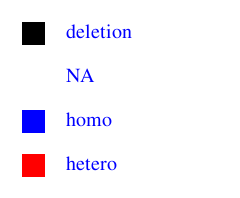
\includegraphics{figures/2010pcr_with_sequenom_149snps_accession2ecotype_complete_y3_legend.png}
\caption{matrix legend}\label{f1}
\end{figure}

\begin{figure}
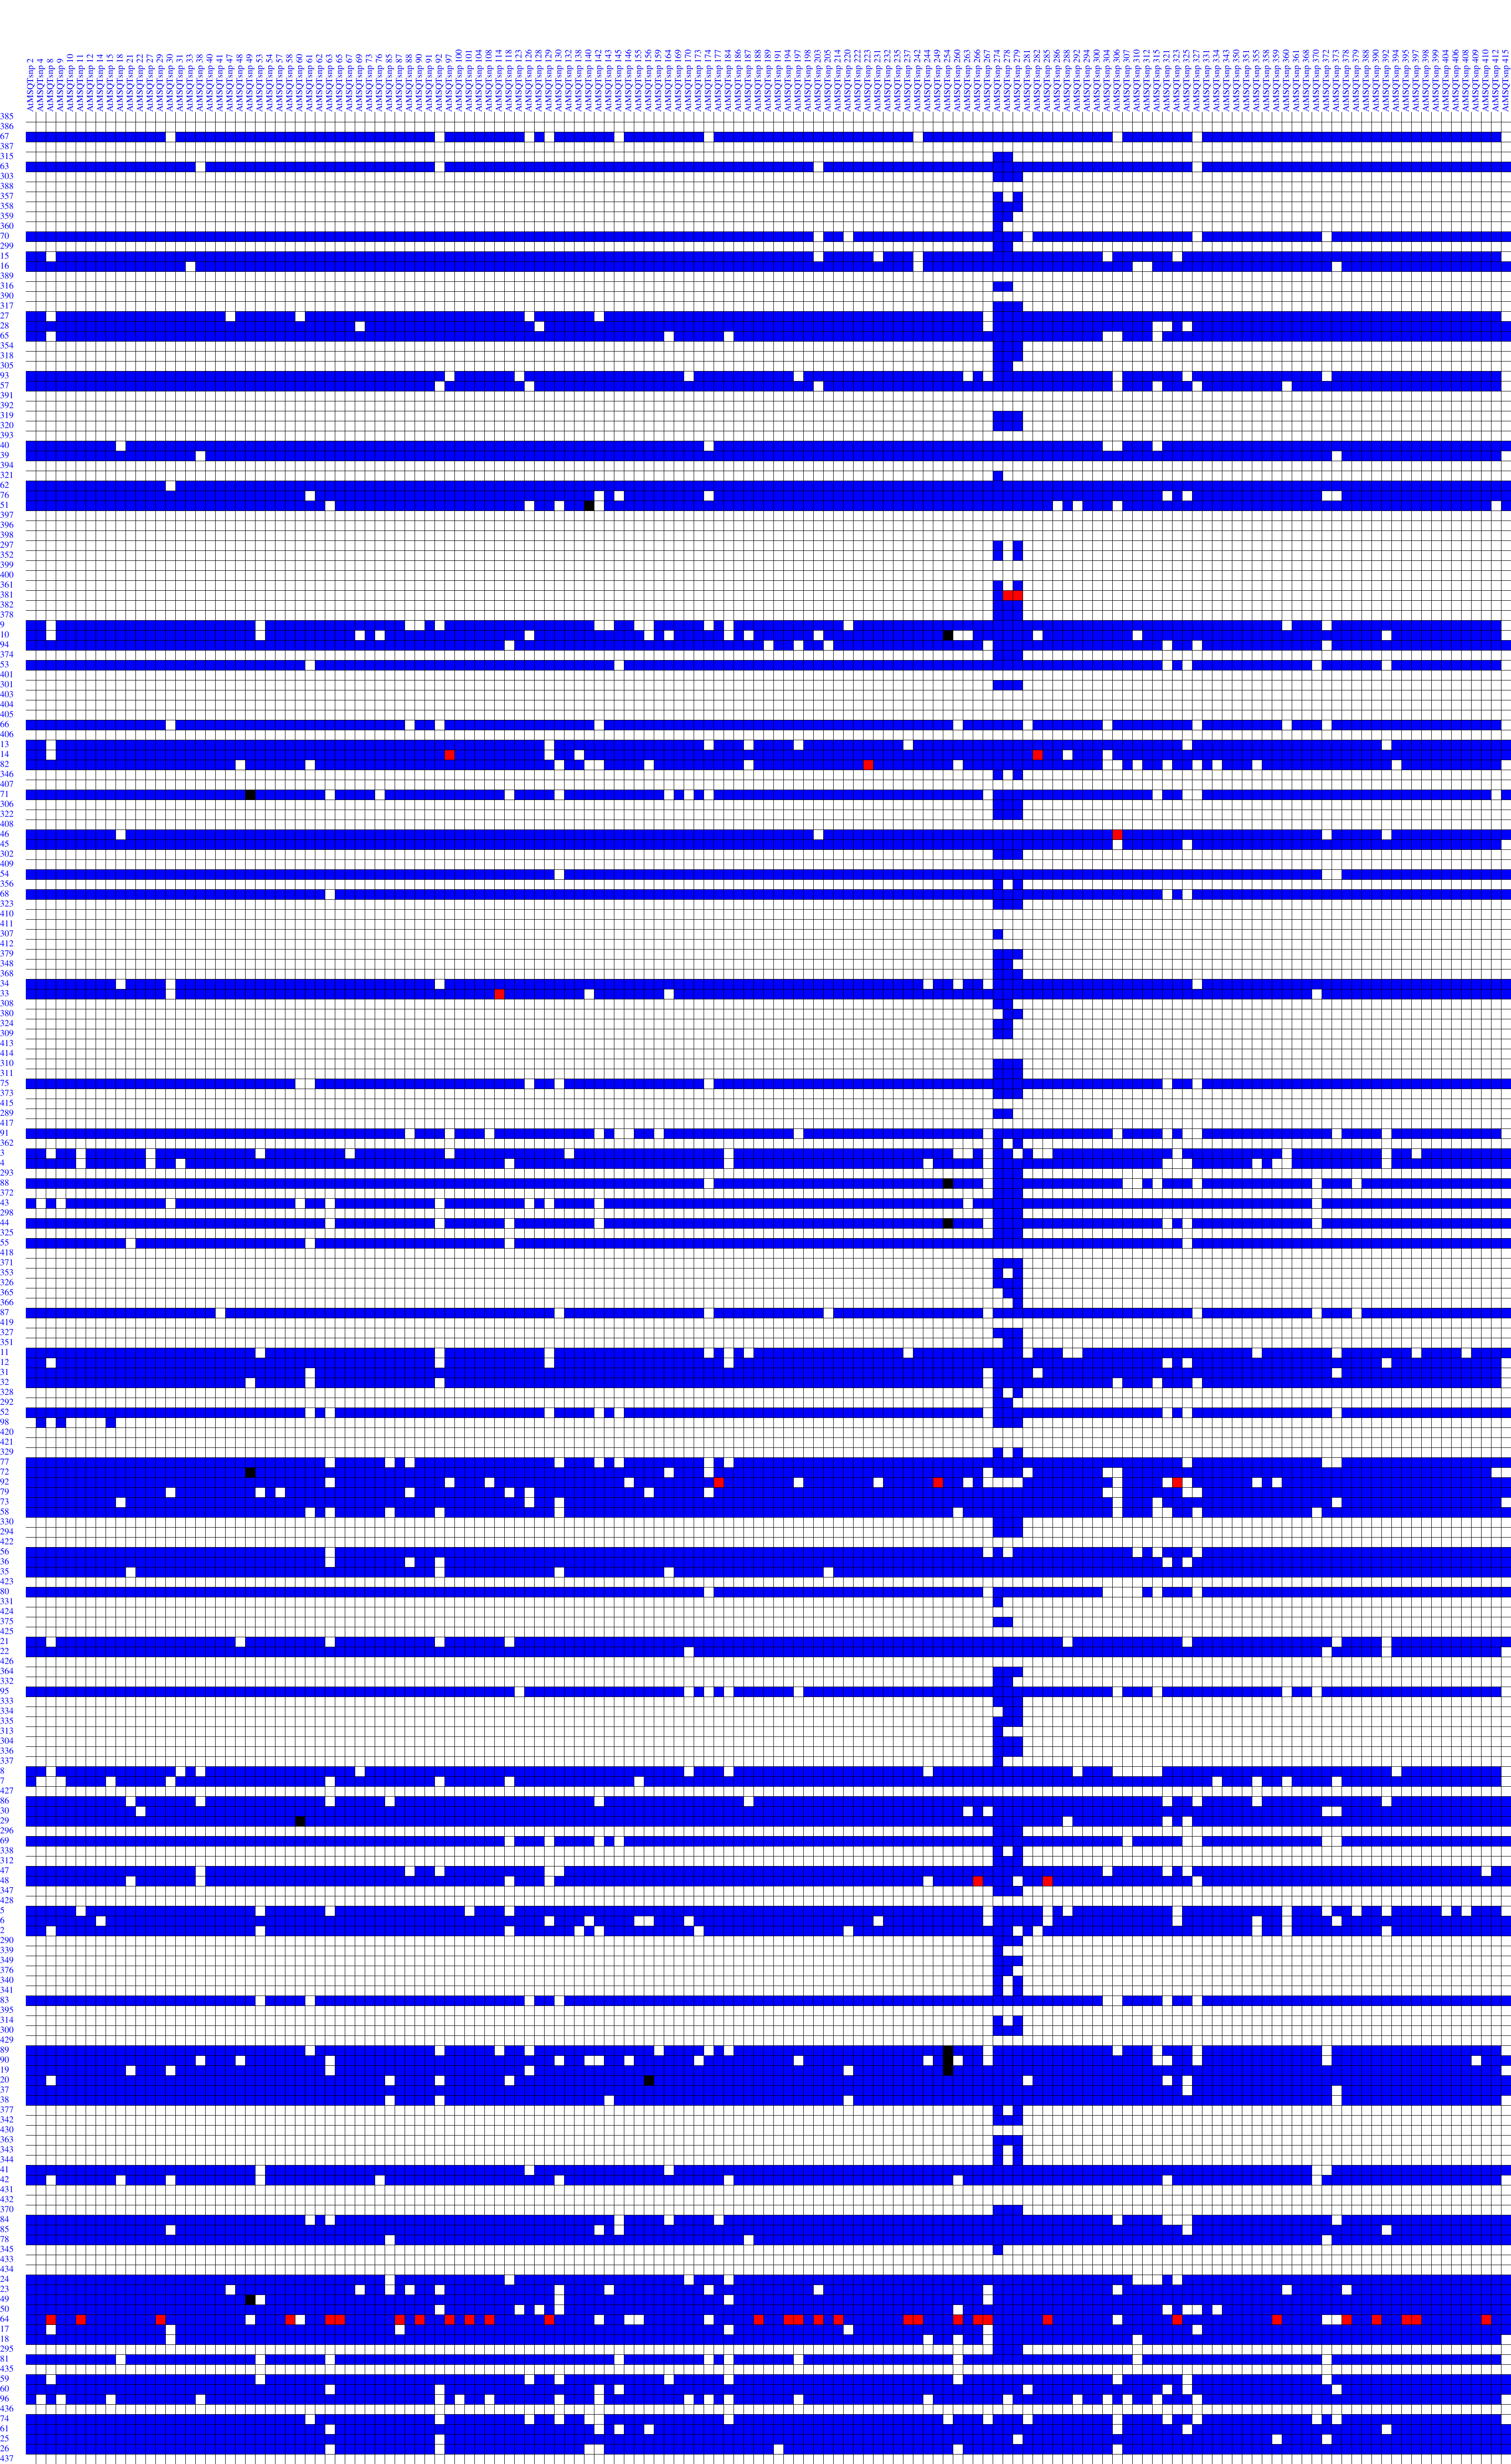
\includegraphics[width=1\textwidth,height=1\textheight]{figures/2010pcr_with_sequenom_149snps_accession2ecotype_complete_y3.png}
\caption{2010 pcr strain X snp matrix. rows are labeled by 2010 accession ids. columns are labeled by SNP ids. check Figure~\ref{f1} for legend.}\label{f2}
\end{figure}

\begin{figure}

\includegraphics[width=1\textwidth, height=1\textheight]{figures/sequenom_with_strains_matched_to_2010pcr_accession2ecotype_complete_y3.png}
\caption{sequenom strain X snp matrix. rows are labeled by sequenom ecotype,duplicate pairs. columns are labeled by SNP ids. check Figure~\ref{f1} for legend.}\label{f3}
\end{figure}

\section{Observations}
\subsection{observation from summary comparison}
Results are in section~\ref{section_summary}. Whether there's a strain recorded is one thing, whether that strain was tried using pcr or sequenom is another thing. Based on whether that strain was \textbf{tried} by pcr in 2010 or sequenom, there're 4 combinations between 2010 and sequenom. 4 tables (Table~\ref{table_dm0}-\ref{table_dm3}) correspond to these 4 different combinations. The data of the strains not tried by sequenom are not included. This is why table~\ref{table_dm1} and table~\ref{table_dm3} are empty.

Attention should be focused on Table~\ref{table_dm0}.
\begin{itemize}
 \item There's a dominance of mismatches happening within two purine (A and G) or two pyrimidine bases (C and T). this is probably related to the mass spectrometry technology used by sequenom.
\item Only 3 heterozygous calls match between 2010 pcr and sequenom data. If the heterozygous call is mismatched, it's mismatched to one of the two alleles (which is nothing new).
\item Check 2nd column, Lots of calls (about 12\% for each base) made in 2010 pcr were called 'NA'(undecided) in sequenom data.
\end{itemize}

All these call for the improvement in the genotype calling algorithm.

\subsection{observation from strain-wise comparison}
Results are in section~\ref{section_strain_wise}.

Strains are ordered by 2010 accession id. For each 2010 strain, different sequenom runs are listed as subsections.

\begin{itemize}
 \item 4 copies of Mr-0 in sequenom. 3 of them show consistent homozygous states. the 3rd one, which is a technical duplicate of the 2nd one, might be contamination (lots of heterozygous calls).
\item 3 copies of Van-0 in sequenom all show consistent homozygous calls in sequenom. but Van-0 shows quite heterozygous in 2010 pcr. So 2010 pcr's Van-0 is contaminated?
\item Cvi-0 looks pretty consistent between two types of data.
\end{itemize}


\subsection{observation from snp-wise comparison}
Results are in section~\ref{section_snp_wise}.

\begin{itemize}
 \item AtMSQTsnp146 has 3 major alleles in 2010 pcr data. In sequenom, the 3rd allele('C') is all called 'NA' except one case.
\item there're 4 bad snps (AtMSQTsnp 138, 232, 263 and 267) showing excessive heterozygosity that were tossed out based on a statistic model. one of them (AtMSQTsnp 264) doesn't show excessive heterozygosity in these strains. AtMSQTsnp 138 has lots of 'C' alleles of 2010 pcr called 'NA' and 'CT' in sequenom data (AtMSQTsnp 232, 267 has similar situation).
\item (loss) snp AtMSQTsnp 30, 33, 47, 58, 60, 61, 67, 87, 91, 92, 129, 155, 156, 164, 170, 184, 186, 189, 205, 214, 231, 235, 237, 286, 331, 360, 368, 372, 398, 406, 409 show calls in 2010 pcr called 'NA' in sequenom data.
\item (recovery) snp AtMSQTsnp 118, 126, 130, 142, 145, 174, 184, 278, 279, 304, 306, 315, 321, 325, 373, 415 show lots of 'NA' in 2010 pcr recovered by sequenom.
\item snp AtMSQTsnp 327, 370, 392 show both loss and recovery.

\end{itemize}



\section{2010 PCR versus sequenom. summary} \label{section_summary}
\begin{center}
\begin{longtable}{|l|l|l|l|l|l|l|l|l|l|l|l|l|}
\caption{PCR-tried vs sequenom-tried} \label{table_dm0}\\
\hline
\\
\hline
&-&NA&A&C&G&T&AC&AG&AT&CG&CT&GT\\
-&0&8&1&0&0&3&0&0&0&0&0&0\\
NA&0&177&150&142&150&122&1&0&0&0&2&0\\
A&0&873&2954&3&23&3&0&0&0&0&0&0\\
C&0&666&8&2402&2&13&0&0&0&0&5&0\\
G&0&866&23&5&2997&5&0&0&0&0&0&0\\
T&0&540&3&18&6&2792&0&0&0&0&0&0\\
AC&0&0&2&0&0&0&0&0&0&0&0&0\\
AG&0&1&10&0&5&0&0&0&0&0&0&0\\
AT&0&0&2&0&0&1&0&0&1&0&0&0\\
CG&0&1&0&3&1&0&0&0&0&0&0&0\\
CT&0&1&0&5&0&4&0&0&0&0&1&0\\
GT&0&1&0&0&1&2&0&0&0&0&0&0\\
\hline
\end{longtable}
\end{center}

\begin{center}
\begin{longtable}{|l|l|l|l|l|l|l|l|l|l|l|l|l|}
\caption{PCR-tried vs sequenom-untried} \label{table_dm1}\\
\hline
\\
\hline
&-&NA&A&C&G&T&AC&AG&AT&CG&CT&GT\\
-&0&0&0&0&0&0&0&0&0&0&0&0\\
NA&0&0&0&0&0&0&0&0&0&0&0&0\\
A&0&0&0&0&0&0&0&0&0&0&0&0\\
C&0&0&0&0&0&0&0&0&0&0&0&0\\
G&0&0&0&0&0&0&0&0&0&0&0&0\\
T&0&0&0&0&0&0&0&0&0&0&0&0\\
AC&0&0&0&0&0&0&0&0&0&0&0&0\\
AG&0&0&0&0&0&0&0&0&0&0&0&0\\
AT&0&0&0&0&0&0&0&0&0&0&0&0\\
CG&0&0&0&0&0&0&0&0&0&0&0&0\\
CT&0&0&0&0&0&0&0&0&0&0&0&0\\
GT&0&0&0&0&0&0&0&0&0&0&0&0\\
\hline
\end{longtable}
\end{center}

\begin{center}
\begin{longtable}{|l|l|l|l|l|l|l|l|l|l|l|l|l|}
\caption{PCR-untried vs sequenom-tried} \label{table_dm2}\\
\hline
\\
\hline
&-&NA&A&C&G&T&AC&AG&AT&CG&CT&GT\\
-&0&0&0&0&0&0&0&0&0&0&0&0\\
NA&0&3081&5098&4220&5114&4463&22&20&7&5&60&6\\
A&0&0&0&0&0&0&0&0&0&0&0&0\\
C&0&0&0&0&0&0&0&0&0&0&0&0\\
G&0&0&0&0&0&0&0&0&0&0&0&0\\
T&0&0&0&0&0&0&0&0&0&0&0&0\\
AC&0&0&0&0&0&0&0&0&0&0&0&0\\
AG&0&0&0&0&0&0&0&0&0&0&0&0\\
AT&0&0&0&0&0&0&0&0&0&0&0&0\\
CG&0&0&0&0&0&0&0&0&0&0&0&0\\
CT&0&0&0&0&0&0&0&0&0&0&0&0\\
GT&0&0&0&0&0&0&0&0&0&0&0&0\\
\hline
\end{longtable}
\end{center}

\begin{center}
\begin{longtable}{|l|l|l|l|l|l|l|l|l|l|l|l|l|}
\caption{PCR-untried vs sequenom-untried} \label{table_dm3}\\
\hline
\\
\hline
&-&NA&A&C&G&T&AC&AG&AT&CG&CT&GT\\
-&0&0&0&0&0&0&0&0&0&0&0&0\\
NA&0&0&0&0&0&0&0&0&0&0&0&0\\
A&0&0&0&0&0&0&0&0&0&0&0&0\\
C&0&0&0&0&0&0&0&0&0&0&0&0\\
G&0&0&0&0&0&0&0&0&0&0&0&0\\
T&0&0&0&0&0&0&0&0&0&0&0&0\\
AC&0&0&0&0&0&0&0&0&0&0&0&0\\
AG&0&0&0&0&0&0&0&0&0&0&0&0\\
AT&0&0&0&0&0&0&0&0&0&0&0&0\\
CG&0&0&0&0&0&0&0&0&0&0&0&0\\
CT&0&0&0&0&0&0&0&0&0&0&0&0\\
GT&0&0&0&0&0&0&0&0&0&0&0&0\\
\hline
\end{longtable}
\end{center}

\section{Real Mismatches between pcr and sequenom (deletion/NA excluded)} \label{section_real_mismatch}
\begin{center}
\begin{longtable}{|l|l|l|l|l|l|l|l|l|l|l|l|}
\caption{mismatches between pcr and sequenom data (deletion/NA excluded, sorted by accession id)} \label{table_dm3}\\
\hline
nativename&stkparent&ecotype\_id&duplicate&accession\_id&SNP&chromosome&position&alignment\_id&alignment\_start&pcr\_call&sequenom\_call\\
\hline
RRS-10&CS22565&8372&1&2&AtMSQTsnp 140&2&8750047&1072&8749828&C&A\\
Kno-10&CS22566&8317&1&3&AtMSQTsnp 378&5&17171676&1489&17171242&G&C\\
L�v-1&CS22574&6043&1&11&AtMSQTsnp 370&5&15065196&756&15065018&A&G\\
L�v-5&CS22575&6046&1&12&AtMSQTsnp 370&5&15065196&756&15065018&A&G\\
F�b-4&CS22577&8293&1&14&AtMSQTsnp 307&4&17038400&2205&17038096&T&A\\
F�b-4&CS22577&8293&1&14&AtMSQTsnp 97&1&24893649&1428&24893448&CG&C\\
Bil-7&CS22579&8263&1&16&AtMSQTsnp 370&5&15065196&756&15065018&A&G\\
�m�2-3&CS22585&8350&1&22&AtMSQTsnp 373&5&15767945&1190&15767914&A&G\\
Zdr-1&CS22588&8409&1&25&AtMSQTsnp 260&4&5775707&933&5775541&C&A\\
Bor-1&CS22590&5837&1&27&AtMSQTsnp 2&1&112907&847&112445&A&G\\
Bor-1&CS22590&5837&1&27&AtMSQTsnp 12&1&2211033&964&2210982&A&G\\
Bor-1&CS22590&5837&1&27&AtMSQTsnp 88&1&23395010&1071&23394478&A&G\\
Bor-1&CS22590&5837&1&27&AtMSQTsnp 100&1&25717887&1758&25717715&A&G\\
Bor-1&CS22590&5837&1&27&AtMSQTsnp 177&2&17859964&118&17859576&A&G\\
Bor-1&CS22590&5837&1&27&AtMSQTsnp 249&4&1055234&482&1055093&A&G\\
Bor-1&CS22590&5837&1&27&AtMSQTsnp 300&4&15765120&1685&15764920&A&G\\
Bor-1&CS22590&5837&1&27&AtMSQTsnp 323&5&872350&532&872097&A&G\\
Bor-1&CS22590&5837&1&27&AtMSQTsnp 358&5&7279057&550&7278798&A&G\\
Bor-1&CS22590&5837&1&27&AtMSQTsnp 368&5&14216131&1035&14215995&A&G\\
Bor-1&CS22590&5837&1&27&AtMSQTsnp 410&5&26120955&596&26120843&A&G\\
Bor-1&CS22590&5837&1&27&AtMSQTsnp 187&3&580470&55&580026&A&T\\
Bor-1&CS22590&5837&1&27&AtMSQTsnp 194&3&3679541&1632&3679103&A&T\\
Bor-1&CS22590&5837&1&27&AtMSQTsnp 191&3&2236458&2592&2236406&C&A\\
Bor-1&CS22590&5837&1&27&AtMSQTsnp 254&4&2441217&233&2440917&C&A\\
Bor-1&CS22590&5837&1&27&AtMSQTsnp 310&4&17608924&1999&17608717&C&A\\
Bor-1&CS22590&5837&1&27&AtMSQTsnp 321&5&625679&2386&625179&C&A\\
Bor-1&CS22590&5837&1&27&AtMSQTsnp 388&5&19316200&761&19315950&C&A\\
Bor-1&CS22590&5837&1&27&AtMSQTsnp 286&4&11580143&1019&11579700&C&G\\
Bor-1&CS22590&5837&1&27&AtMSQTsnp 398&5&22116788&642&22116605&C&G\\
Bor-1&CS22590&5837&1&27&AtMSQTsnp 21&1&4142539&2625&4142402&C&T\\
Bor-1&CS22590&5837&1&27&AtMSQTsnp 30&1&5629159&2156&5628596&C&T\\
Bor-1&CS22590&5837&1&27&AtMSQTsnp 343&5&3606967&538&3606683&C&T\\
Bor-1&CS22590&5837&1&27&AtMSQTsnp 22&1&4396087&46&4395913&G&A\\
Bor-1&CS22590&5837&1&27&AtMSQTsnp 67&1&17355738&660&17355484&G&A\\
Bor-1&CS22590&5837&1&27&AtMSQTsnp 91&1&24071689&1427&24071203&G&A\\
Bor-1&CS22590&5837&1&27&AtMSQTsnp 92&1&24292774&672&24292482&G&A\\
Bor-1&CS22590&5837&1&27&AtMSQTsnp 123&2&1798445&2109&1798324&G&A\\
Bor-1&CS22590&5837&1&27&AtMSQTsnp 129&2&5804076&407&5803805&G&A\\
Bor-1&CS22590&5837&1&27&AtMSQTsnp 220&3&11398207&1053&11398071&G&A\\
Bor-1&CS22590&5837&1&27&AtMSQTsnp 223&3&16489589&2208&16489217&G&A\\
Bor-1&CS22590&5837&1&27&AtMSQTsnp 278&4&9377790&2783&9377549&G&A\\
Bor-1&CS22590&5837&1&27&AtMSQTsnp 288&4&11984772&1376&11984495&G&A\\
Bor-1&CS22590&5837&1&27&AtMSQTsnp 370&5&15065196&756&15065018&G&A\\
Bor-1&CS22590&5837&1&27&AtMSQTsnp 373&5&15767945&1190&15767914&G&A\\
Bor-1&CS22590&5837&1&27&AtMSQTsnp 379&5&17629384&2039&17629093&G&A\\
Bor-1&CS22590&5837&1&27&AtMSQTsnp 394&5&20518330&2759&20518241&G&A\\
Bor-1&CS22590&5837&1&27&AtMSQTsnp 406&5&23815848&978&23815354&G&A\\
Bor-1&CS22590&5837&1&27&AtMSQTsnp 408&5&25301234&2690&25300706&G&A\\
Bor-1&CS22590&5837&1&27&AtMSQTsnp 40&1&7842523&928&7842440&G&C\\
Bor-1&CS22590&5837&1&27&AtMSQTsnp 58&1&12093546&279&12093079&G&C\\
Bor-1&CS22590&5837&1&27&AtMSQTsnp 97&1&24893649&1428&24893448&G&C\\
Bor-1&CS22590&5837&1&27&AtMSQTsnp 31&1&5923041&265&5922974&G&T\\
Bor-1&CS22590&5837&1&27&AtMSQTsnp 184&2&18752840&1423&18752604&T&A\\
Bor-1&CS22590&5837&1&27&AtMSQTsnp 48&1&9497118&930&9496666&T&C\\
Bor-1&CS22590&5837&1&27&AtMSQTsnp 49&1&9781347&1018&9781260&T&C\\
Bor-1&CS22590&5837&1&27&AtMSQTsnp 57&1&11655519&273&11655171&T&C\\
Bor-1&CS22590&5837&1&27&AtMSQTsnp 76&1&21908667&2670&21908157&T&C\\
Bor-1&CS22590&5837&1&27&AtMSQTsnp 130&2&6499679&2098&6499196&T&C\\
Bor-1&CS22590&5837&1&27&AtMSQTsnp 145&2&10566917&381&10566416&T&C\\
Bor-1&CS22590&5837&1&27&AtMSQTsnp 159&2&13265124&2127&13265029&T&C\\
Bor-1&CS22590&5837&1&27&AtMSQTsnp 188&3&2072780&649&2072648&T&C\\
Bor-1&CS22590&5837&1&27&AtMSQTsnp 263&4&7077926&495&7077771&T&C\\
Bor-1&CS22590&5837&1&27&AtMSQTsnp 325&5&1214057&2388&1213621&T&C\\
Bor-1&CS22590&5837&1&27&AtMSQTsnp 390&5&20215473&970&20214933&T&C\\
Bor-1&CS22590&5837&1&27&AtMSQTsnp 294&4&13576588&960&13576336&T&G\\
Bor-1&CS22590&5837&1&27&AtMSQTsnp 355&5&6708014&547&6707732&T&G\\
HR-5&CS22596&8309&1&33&AtMSQTsnp 114&1&30214313&1800&30213917&AG&A\\
NFA-10&CS22599&8345&1&36&AtMSQTsnp 159&2&13265124&2127&13265029&C&T\\
CIBC-5&CS22602&8277&1&39&AtMSQTsnp 321&5&625679&2386&625179&A&C\\
CIBC-5&CS22602&8277&1&39&AtMSQTsnp 223&3&16489589&2208&16489217&A&G\\
CIBC-5&CS22602&8277&1&39&AtMSQTsnp 244&3&23053878&1662&23053771&A&G\\
CIBC-5&CS22602&8277&1&39&AtMSQTsnp 304&4&16272521&2262&16272270&C&T\\
CIBC-5&CS22602&8277&1&39&AtMSQTsnp 334&5&2244739&1995&2244524&C&T\\
CIBC-5&CS22602&8277&1&39&AtMSQTsnp 138&2&8371133&373&8370574&C&CT\\
CIBC-5&CS22602&8277&1&39&AtMSQTsnp 306&4&16742071&2714&16741855&G&C\\
CIBC-5&CS22602&8277&1&39&AtMSQTsnp 307&4&17038400&2205&17038096&T&A\\
CIBC-17&CS22603&8276&1&40&AtMSQTsnp 415&5&26708459&2711&26707937&A&G\\
CIBC-17&CS22603&8276&1&40&AtMSQTsnp 307&4&17038400&2205&17038096&A&T\\
CIBC-17&CS22603&8276&1&40&AtMSQTsnp 321&5&625679&2386&625179&C&A\\
CIBC-17&CS22603&8276&1&40&AtMSQTsnp 159&2&13265124&2127&13265029&C&T\\
CIBC-17&CS22603&8276&1&40&AtMSQTsnp 114&1&30214313&1800&30213917&G&A\\
CIBC-17&CS22603&8276&1&40&AtMSQTsnp 223&3&16489589&2208&16489217&G&A\\
CIBC-17&CS22603&8276&1&40&AtMSQTsnp 244&3&23053878&1662&23053771&G&A\\
CIBC-17&CS22603&8276&1&40&AtMSQTsnp 327&5&1497133&2105&1496987&G&T\\
CIBC-17&CS22603&8276&1&40&AtMSQTsnp 334&5&2244739&1995&2244524&T&C\\
Kz-1&CS22606&8320&1&43&AtMSQTsnp 15&1&2844525&1139&2844111&T&C\\
Got-22&CS22609&8298&1&46&AtMSQTsnp 306&4&16742071&2714&16741855&CG&G\\
Ren-1&CS22610&8367&1&47&AtMSQTsnp 388&5&19316200&761&19315950&A&C\\
Lz-0&CS22615&8336&1&52&AtMSQTsnp 159&2&13265124&2127&13265029&T&C\\
Ler-1&CS22618&8324&1&55&AtMSQTsnp 159&2&13265124&2127&13265029&T&C\\
C24&CS22620&8273&1&57&AtMSQTsnp 138&2&8371133&373&8370574&C&CT\\
Yo-0&CS22624&8408&1&61&AtMSQTsnp 138&2&8371133&373&8370574&C&CT\\
Van-0&CS22627&8400&1&64&AtMSQTsnp 281&4&10482088&956&10482038&C&T\\
Van-0&CS22627&8400&1&64&AtMSQTsnp 12&1&2211033&964&2210982&G&A\\
Van-0&CS22627&8400&1&64&AtMSQTsnp 220&3&11398207&1053&11398071&G&A\\
Van-0&CS22627&8400&1&64&AtMSQTsnp 63&1&13712241&345&13711856&AC&A\\
Van-0&CS22627&8400&1&64&AtMSQTsnp 260&4&5775707&933&5775541&AC&A\\
Van-0&CS22627&8400&1&64&AtMSQTsnp 65&1&16874727&290&16874305&AG&A\\
Van-0&CS22627&8400&1&64&AtMSQTsnp 101&1&26278413&330&26278221&AG&A\\
Van-0&CS22627&8400&1&64&AtMSQTsnp 197&3&4818602&435&4818362&AG&A\\
Van-0&CS22627&8400&1&64&AtMSQTsnp 214&3&9747261&641&9747158&AG&A\\
Van-0&CS22627&8400&1&64&AtMSQTsnp 323&5&872350&532&872097&AG&A\\
Van-0&CS22627&8400&1&64&AtMSQTsnp 395&5&20915321&981&20915132&AG&A\\
Van-0&CS22627&8400&1&64&AtMSQTsnp 8&1&993374&1042&992824&AG&G\\
Van-0&CS22627&8400&1&64&AtMSQTsnp 108&1&28666837&343&28666569&AG&G\\
Van-0&CS22627&8400&1&64&AtMSQTsnp 410&5&26120955&596&26120843&AG&G\\
Van-0&CS22627&8400&1&64&AtMSQTsnp 29&1&5482008&263&5481722&AT&A\\
Van-0&CS22627&8400&1&64&AtMSQTsnp 203&3&6890665&73&6890596&AT&A\\
Van-0&CS22627&8400&1&64&AtMSQTsnp 194&3&3679541&1632&3679103&AT&T\\
Van-0&CS22627&8400&1&64&AtMSQTsnp 97&1&24893649&1428&24893448&CG&C\\
Van-0&CS22627&8400&1&64&AtMSQTsnp 378&5&17171676&1489&17171242&CG&C\\
Van-0&CS22627&8400&1&64&AtMSQTsnp 87&1&23381760&312&23381443&CT&C\\
Van-0&CS22627&8400&1&64&AtMSQTsnp 90&1&23893336&69&23893276&CT&C\\
Van-0&CS22627&8400&1&64&AtMSQTsnp 188&3&2072780&649&2072648&CT&C\\
Van-0&CS22627&8400&1&64&AtMSQTsnp 242&3&21632608&138&21632379&CT&C\\
Van-0&CS22627&8400&1&64&AtMSQTsnp 267&4&8297960&499&8297594&CT&C\\
Van-0&CS22627&8400&1&64&AtMSQTsnp 11&1&1602136&848&1601885&CT&T\\
Van-0&CS22627&8400&1&64&AtMSQTsnp 285&4&11326190&507&11325921&CT&T\\
Van-0&CS22627&8400&1&64&AtMSQTsnp 390&5&20215473&970&20214933&CT&T\\
Van-0&CS22627&8400&1&64&AtMSQTsnp 359&5&7442381&1363&7442039&GT&G\\
Van-0&CS22627&8400&1&64&AtMSQTsnp 266&4&8078648&238&8078388&GT&T\\
Van-0&CS22627&8400&1&64&AtMSQTsnp 397&5&22040877&992&22040690&GT&T\\
Ra-0&CS22632&8364&1&69&AtMSQTsnp 321&5&625679&2386&625179&A&C\\
Ra-0&CS22632&8364&1&69&AtMSQTsnp 334&5&2244739&1995&2244524&C&T\\
Ra-0&CS22632&8364&1&69&AtMSQTsnp 223&3&16489589&2208&16489217&G&A\\
Mrk-0&CS22635&8339&1&72&AtMSQTsnp 325&5&1214057&2388&1213621&C&T\\
Wt-5&CS22637&8407&1&74&AtMSQTsnp 334&5&2244739&1995&2244524&T&C\\
Ct-1&CS22639&8280&1&76&AtMSQTsnp 292&4&12404111&2534&12403706&T&C\\
Tsu-1&CS22641&8394&1&78&AtMSQTsnp 138&2&8371133&373&8370574&C&T\\
Tsu-1&CS22641&8394&1&78&AtMSQTsnp 334&5&2244739&1995&2244524&T&C\\
Mt-0&CS22642&8341&1&79&AtMSQTsnp 138&2&8371133&373&8370574&C&CT\\
Nok-3&CS22643&8347&1&80&AtMSQTsnp 334&5&2244739&1995&2244524&C&T\\
Fei-0&CS22645&8294&1&82&AtMSQTsnp 223&3&16489589&2208&16489217&AG&G\\
Kondara&CS22651&8319&1&88&AtMSQTsnp 114&1&30214313&1800&30213917&A&G\\
Kin-0&CS22654&8316&1&91&AtMSQTsnp 138&2&8371133&373&8370574&C&CT\\
Ms-0&CS22655&8340&1&92&AtMSQTsnp 173&2&16908190&728&16908054&A&G\\
Ms-0&CS22655&8340&1&92&AtMSQTsnp 177&2&17859964&118&17859576&AG&A\\
Ms-0&CS22655&8340&1&92&AtMSQTsnp 249&4&1055234&482&1055093&AG&A\\
Ms-0&CS22655&8340&1&92&AtMSQTsnp 323&5&872350&532&872097&AG&G\\
NC-6&&8246&1&294&AtMSQTsnp 278&4&9377790&2783&9377549&G&A\\
NC-6&&8246&1&294&AtMSQTsnp 274&4&9213312&2778&9213072&T&G\\
Sf-1&N6855&8380&1&300&AtMSQTsnp 278&4&9377790&2783&9377549&A&G\\
Sf-1&N6855&8380&1&300&AtMSQTsnp 274&4&9213312&2778&9213072&G&T\\
PHW-34&N6034&8244&1&304&AtMSQTsnp 274&4&9213312&2778&9213072&T&G\\
Pi-0&N1455&8356&1&336&AtMSQTsnp 279&4&9580049&2788&9579976&C&T\\
Pi-0&N1455&8356&1&336&AtMSQTsnp 274&4&9213312&2778&9213072&T&G\\
Lom1-1&&6042&2&351&AtMSQTsnp 278&4&9377790&2783&9377549&A&G\\
Gul1-2&&8234&1&356&AtMSQTsnp 274&4&9213312&2778&9213072&G&T\\
Stu1-1&&6088&1&363&AtMSQTsnp 274&4&9213312&2778&9213072&G&T\\
Duk&&6008&2&378&AtMSQTsnp 278&4&9377790&2783&9377549&A&G\\
DraII-1&&8284&1&381&AtMSQTsnp 274&4&9213312&2778&9213072&T&G\\
DraII-1&&8284&1&381&AtMSQTsnp 278&4&9377790&2783&9377549&AG&A\\
DraII-1&&8284&1&381&AtMSQTsnp 279&4&9580049&2788&9579976&CT&T\\
\hline
\end{longtable}
\end{center}

\section{2010 PCR versus sequenom for each strain} \label{section_strain_wise}
\subsection{strain RRS-10(accession id=2)}
\subsubsection{corresponding ecotype RRS-10(stkparent=CS22565, ecotype id=8372, duplicate=1)}
\begin{center}
\begin{longtable}{|l|l|l|l|l|l|l|l|l|l|l|l|l|}
\caption{accession id=2 vs ecotype id=8372, duplicate=1(nativename=RRS-10, stockparent=CS22565)} \label{table_dm4}\\
\hline
\\
\hline
&-&NA&A&C&G&T&AC&AG&AT&CG&CT&GT\\
-&0&0&0&0&0&0&0&0&0&0&0&0\\
NA&0&1&2&0&3&3&0&0&0&0&0&0\\
A&0&10&32&0&0&0&0&0&0&0&0&0\\
C&0&4&1&22&0&0&0&0&0&0&0&0\\
G&0&7&0&0&28&0&0&0&0&0&0&0\\
T&0&4&0&0&0&29&0&0&0&0&0&0\\
AC&0&0&0&0&0&0&0&0&0&0&0&0\\
AG&0&0&0&0&0&0&0&0&0&0&0&0\\
AT&0&0&0&0&0&0&0&0&0&0&0&0\\
CG&0&0&0&0&0&0&0&0&0&0&0&0\\
CT&0&0&0&0&0&0&0&0&0&0&0&0\\
GT&0&0&0&0&0&0&0&0&0&0&0&0\\
\hline
\end{longtable}
\end{center}

\begin{center}
\begin{longtable}{|l|l|l|l|l|l|l|}
\caption{detailed difference for accession id=2 vs ecotype id=8372, duplicate=1} \label{table_dm5}\\
\hline
snp&chromosome&position&alignment\_id&alignment\_start&pcr\_call&sequenom\_call\\
\hline
AtMSQTsnp 8&1&993374&1042&992824&NA&A\\
AtMSQTsnp 27&1&5206767&1014&5206479&A&NA\\
AtMSQTsnp 30&1&5629159&2156&5628596&C&NA\\
AtMSQTsnp 33&1&6375605&967&6375563&T&NA\\
AtMSQTsnp 47&1&9343401&929&9343234&C&NA\\
AtMSQTsnp 53&1&10423708&948&10423483&NA&T\\
AtMSQTsnp 58&1&12093546&279&12093079&G&NA\\
AtMSQTsnp 60&1&12357583&1973&12357044&A&NA\\
AtMSQTsnp 67&1&17355738&660&17355484&G&NA\\
AtMSQTsnp 91&1&24071689&1427&24071203&A&NA\\
AtMSQTsnp 92&1&24292774&672&24292482&G&NA\\
AtMSQTsnp 118&2&322335&2465&322253&NA&G\\
AtMSQTsnp 129&2&5804076&407&5803805&G&NA\\
AtMSQTsnp 140&2&8750047&1072&8749828&C&A\\
AtMSQTsnp 142&2&9256095&223&9256049&NA&T\\
AtMSQTsnp 155&2&12657149&38&12656716&G&NA\\
AtMSQTsnp 156&2&12658862&2572&12658576&T&NA\\
AtMSQTsnp 164&2&14003409&2631&14003272&A&NA\\
AtMSQTsnp 170&2&15986354&2292&15986145&C&NA\\
AtMSQTsnp 173&2&16908190&728&16908054&NA&G\\
AtMSQTsnp 184&2&18752840&1423&18752604&T&NA\\
AtMSQTsnp 186&3&298210&777&297801&A&NA\\
AtMSQTsnp 189&3&2231938&779&2231413&A&NA\\
AtMSQTsnp 205&3&7392098&91&7391896&C&NA\\
AtMSQTsnp 220&3&11398207&1053&11398071&NA&A\\
AtMSQTsnp 235&3&19930624&833&19930188&A&NA\\
AtMSQTsnp 278&4&9377790&2783&9377549&A&NA\\
AtMSQTsnp 279&4&9580049&2788&9579976&NA&T\\
AtMSQTsnp 286&4&11580143&1019&11579700&G&NA\\
AtMSQTsnp 327&5&1497133&2105&1496987&T&NA\\
AtMSQTsnp 331&5&1931167&1633&1931083&G&NA\\
AtMSQTsnp 368&5&14216131&1035&14215995&A&NA\\
AtMSQTsnp 392&5&20409250&994&20408706&NA&G\\
AtMSQTsnp 406&5&23815848&978&23815354&A&NA\\
\hline
\end{longtable}
\end{center}

\subsection{strain Kno-10(accession id=3)}
\subsubsection{corresponding ecotype Kno-10(stkparent=CS22566, ecotype id=8317, duplicate=1)}
\begin{center}
\begin{longtable}{|l|l|l|l|l|l|l|l|l|l|l|l|l|}
\caption{accession id=3 vs ecotype id=8317, duplicate=1(nativename=Kno-10, stockparent=CS22566)} \label{table_dm6}\\
\hline
\\
\hline
&-&NA&A&C&G&T&AC&AG&AT&CG&CT&GT\\
-&0&0&0&0&0&0&0&0&0&0&0&0\\
NA&0&3&2&0&1&4&0&0&0&0&0&0\\
A&0&8&34&0&0&0&0&0&0&0&0&0\\
C&0&4&0&18&0&0&0&0&0&0&0&0\\
G&0&6&0&1&29&0&0&0&0&0&0&0\\
T&0&4&0&0&0&27&0&0&0&0&0&0\\
AC&0&0&0&0&0&0&0&0&0&0&0&0\\
AG&0&0&0&0&0&0&0&0&0&0&0&0\\
AT&0&0&0&0&0&0&0&0&0&0&0&0\\
CG&0&0&0&0&0&0&0&0&0&0&0&0\\
CT&0&0&0&0&0&0&0&0&0&0&0&0\\
GT&0&0&0&0&0&0&0&0&0&0&0&0\\
\hline
\end{longtable}
\end{center}

\begin{center}
\begin{longtable}{|l|l|l|l|l|l|l|}
\caption{detailed difference for accession id=3 vs ecotype id=8317, duplicate=1} \label{table_dm7}\\
\hline
snp&chromosome&position&alignment\_id&alignment\_start&pcr\_call&sequenom\_call\\
\hline
AtMSQTsnp 8&1&993374&1042&992824&NA&A\\
AtMSQTsnp 30&1&5629159&2156&5628596&C&NA\\
AtMSQTsnp 33&1&6375605&967&6375563&T&NA\\
AtMSQTsnp 47&1&9343401&929&9343234&C&NA\\
AtMSQTsnp 58&1&12093546&279&12093079&G&NA\\
AtMSQTsnp 60&1&12357583&1973&12357044&A&NA\\
AtMSQTsnp 87&1&23381760&312&23381443&T&NA\\
AtMSQTsnp 91&1&24071689&1427&24071203&A&NA\\
AtMSQTsnp 92&1&24292774&672&24292482&G&NA\\
AtMSQTsnp 129&2&5804076&407&5803805&G&NA\\
AtMSQTsnp 132&2&7072955&367&7072571&NA&T\\
AtMSQTsnp 155&2&12657149&38&12656716&G&NA\\
AtMSQTsnp 156&2&12658862&2572&12658576&T&NA\\
AtMSQTsnp 164&2&14003409&2631&14003272&A&NA\\
AtMSQTsnp 170&2&15986354&2292&15986145&C&NA\\
AtMSQTsnp 186&3&298210&777&297801&A&NA\\
AtMSQTsnp 189&3&2231938&779&2231413&A&NA\\
AtMSQTsnp 205&3&7392098&91&7391896&C&NA\\
AtMSQTsnp 235&3&19930624&833&19930188&A&NA\\
AtMSQTsnp 237&3&20483289&1645&20482976&T&NA\\
AtMSQTsnp 260&4&5775707&933&5775541&NA&A\\
AtMSQTsnp 263&4&7077926&495&7077771&NA&T\\
AtMSQTsnp 279&4&9580049&2788&9579976&NA&T\\
AtMSQTsnp 282&4&10659455&505&10659034&NA&T\\
AtMSQTsnp 286&4&11580143&1019&11579700&G&NA\\
AtMSQTsnp 331&5&1931167&1633&1931083&G&NA\\
AtMSQTsnp 368&5&14216131&1035&14215995&A&NA\\
AtMSQTsnp 378&5&17171676&1489&17171242&G&C\\
AtMSQTsnp 397&5&22040877&992&22040690&NA&G\\
AtMSQTsnp 406&5&23815848&978&23815354&A&NA\\
\hline
\end{longtable}
\end{center}

\subsection{strain Kno-18(accession id=4)}
\subsubsection{corresponding ecotype Kno-18(stkparent=CS22567, ecotype id=8318, duplicate=1)}
\begin{center}
\begin{longtable}{|l|l|l|l|l|l|l|l|l|l|l|l|l|}
\caption{accession id=4 vs ecotype id=8318, duplicate=1(nativename=Kno-18, stockparent=CS22567)} \label{table_dm8}\\
\hline
\\
\hline
&-&NA&A&C&G&T&AC&AG&AT&CG&CT&GT\\
-&0&0&0&0&0&0&0&0&0&0&0&0\\
NA&0&3&2&1&1&2&0&0&0&0&0&0\\
A&0&7&31&0&0&0&0&0&0&0&0&0\\
C&0&3&0&23&0&0&0&0&0&0&0&0\\
G&0&11&0&0&26&0&0&0&0&0&0&0\\
T&0&5&0&0&0&29&0&0&0&0&0&0\\
AC&0&0&0&0&0&0&0&0&0&0&0&0\\
AG&0&0&0&0&0&0&0&0&0&0&0&0\\
AT&0&0&0&0&0&0&0&0&0&0&0&0\\
CG&0&0&0&0&0&0&0&0&0&0&0&0\\
CT&0&0&0&0&0&0&0&0&0&0&0&0\\
GT&0&0&0&0&0&0&0&0&0&0&0&0\\
\hline
\end{longtable}
\end{center}

\begin{center}
\begin{longtable}{|l|l|l|l|l|l|l|}
\caption{detailed difference for accession id=4 vs ecotype id=8318, duplicate=1} \label{table_dm9}\\
\hline
snp&chromosome&position&alignment\_id&alignment\_start&pcr\_call&sequenom\_call\\
\hline
AtMSQTsnp 11&1&1602136&848&1601885&NA&C\\
AtMSQTsnp 30&1&5629159&2156&5628596&C&NA\\
AtMSQTsnp 31&1&5923041&265&5922974&NA&G\\
AtMSQTsnp 33&1&6375605&967&6375563&T&NA\\
AtMSQTsnp 47&1&9343401&929&9343234&C&NA\\
AtMSQTsnp 58&1&12093546&279&12093079&G&NA\\
AtMSQTsnp 60&1&12357583&1973&12357044&A&NA\\
AtMSQTsnp 61&1&13395892&1673&13395451&C&NA\\
AtMSQTsnp 67&1&17355738&660&17355484&G&NA\\
AtMSQTsnp 87&1&23381760&312&23381443&T&NA\\
AtMSQTsnp 91&1&24071689&1427&24071203&G&NA\\
AtMSQTsnp 92&1&24292774&672&24292482&G&NA\\
AtMSQTsnp 118&2&322335&2465&322253&NA&A\\
AtMSQTsnp 129&2&5804076&407&5803805&G&NA\\
AtMSQTsnp 155&2&12657149&38&12656716&G&NA\\
AtMSQTsnp 156&2&12658862&2572&12658576&T&NA\\
AtMSQTsnp 164&2&14003409&2631&14003272&A&NA\\
AtMSQTsnp 170&2&15986354&2292&15986145&A&NA\\
AtMSQTsnp 186&3&298210&777&297801&A&NA\\
AtMSQTsnp 189&3&2231938&779&2231413&G&NA\\
AtMSQTsnp 205&3&7392098&91&7391896&T&NA\\
AtMSQTsnp 232&3&18980664&829&18980171&A&NA\\
AtMSQTsnp 235&3&19930624&833&19930188&G&NA\\
AtMSQTsnp 286&4&11580143&1019&11579700&G&NA\\
AtMSQTsnp 321&5&625679&2386&625179&NA&A\\
AtMSQTsnp 325&5&1214057&2388&1213621&NA&T\\
AtMSQTsnp 327&5&1497133&2105&1496987&T&NA\\
AtMSQTsnp 331&5&1931167&1633&1931083&G&NA\\
AtMSQTsnp 359&5&7442381&1363&7442039&NA&T\\
AtMSQTsnp 368&5&14216131&1035&14215995&A&NA\\
AtMSQTsnp 372&5&15569205&926&15568698&G&NA\\
AtMSQTsnp 406&5&23815848&978&23815354&A&NA\\
\hline
\end{longtable}
\end{center}

\subsection{strain Rmx-A02(accession id=5)}
\subsubsection{corresponding ecotype Rmx-A02(stkparent=CS22568, ecotype id=8370, duplicate=1)}
\begin{center}
\begin{longtable}{|l|l|l|l|l|l|l|l|l|l|l|l|l|}
\caption{accession id=5 vs ecotype id=8370, duplicate=1(nativename=Rmx-A02, stockparent=CS22568)} \label{table_dm10}\\
\hline
\\
\hline
&-&NA&A&C&G&T&AC&AG&AT&CG&CT&GT\\
-&0&0&0&0&0&0&0&0&0&0&0&0\\
NA&0&2&5&0&2&2&0&0&0&0&0&0\\
A&0&8&33&0&0&0&0&0&0&0&0&0\\
C&0&5&0&21&0&0&0&0&0&0&0&0\\
G&0&7&0&0&28&0&0&0&0&0&0&0\\
T&0&6&0&0&0&25&0&0&0&0&0&0\\
AC&0&0&0&0&0&0&0&0&0&0&0&0\\
AG&0&0&0&0&0&0&0&0&0&0&0&0\\
AT&0&0&0&0&0&0&0&0&0&0&0&0\\
CG&0&0&0&0&0&0&0&0&0&0&0&0\\
CT&0&0&0&0&0&0&0&0&0&0&0&0\\
GT&0&0&0&0&0&0&0&0&0&0&0&0\\
\hline
\end{longtable}
\end{center}

\begin{center}
\begin{longtable}{|l|l|l|l|l|l|l|}
\caption{detailed difference for accession id=5 vs ecotype id=8370, duplicate=1} \label{table_dm11}\\
\hline
snp&chromosome&position&alignment\_id&alignment\_start&pcr\_call&sequenom\_call\\
\hline
AtMSQTsnp 27&1&5206767&1014&5206479&A&NA\\
AtMSQTsnp 30&1&5629159&2156&5628596&C&NA\\
AtMSQTsnp 33&1&6375605&967&6375563&T&NA\\
AtMSQTsnp 47&1&9343401&929&9343234&C&NA\\
AtMSQTsnp 53&1&10423708&948&10423483&NA&T\\
AtMSQTsnp 58&1&12093546&279&12093079&G&NA\\
AtMSQTsnp 60&1&12357583&1973&12357044&A&NA\\
AtMSQTsnp 67&1&17355738&660&17355484&G&NA\\
AtMSQTsnp 87&1&23381760&312&23381443&T&NA\\
AtMSQTsnp 91&1&24071689&1427&24071203&A&NA\\
AtMSQTsnp 92&1&24292774&672&24292482&G&NA\\
AtMSQTsnp 101&1&26278413&330&26278221&NA&A\\
AtMSQTsnp 118&2&322335&2465&322253&NA&G\\
AtMSQTsnp 129&2&5804076&407&5803805&G&NA\\
AtMSQTsnp 155&2&12657149&38&12656716&G&NA\\
AtMSQTsnp 156&2&12658862&2572&12658576&T&NA\\
AtMSQTsnp 164&2&14003409&2631&14003272&A&NA\\
AtMSQTsnp 170&2&15986354&2292&15986145&C&NA\\
AtMSQTsnp 184&2&18752840&1423&18752604&T&NA\\
AtMSQTsnp 186&3&298210&777&297801&A&NA\\
AtMSQTsnp 189&3&2231938&779&2231413&A&NA\\
AtMSQTsnp 205&3&7392098&91&7391896&C&NA\\
AtMSQTsnp 235&3&19930624&833&19930188&G&NA\\
AtMSQTsnp 237&3&20483289&1645&20482976&T&NA\\
AtMSQTsnp 286&4&11580143&1019&11579700&C&NA\\
AtMSQTsnp 288&4&11984772&1376&11984495&NA&G\\
AtMSQTsnp 327&5&1497133&2105&1496987&T&NA\\
AtMSQTsnp 331&5&1931167&1633&1931083&G&NA\\
AtMSQTsnp 368&5&14216131&1035&14215995&A&NA\\
AtMSQTsnp 372&5&15569205&926&15568698&NA&A\\
AtMSQTsnp 379&5&17629384&2039&17629093&NA&A\\
AtMSQTsnp 404&5&23270994&1391&23270845&NA&T\\
AtMSQTsnp 406&5&23815848&978&23815354&A&NA\\
AtMSQTsnp 408&5&25301234&2690&25300706&NA&A\\
AtMSQTsnp 415&5&26708459&2711&26707937&NA&A\\
\hline
\end{longtable}
\end{center}

\subsection{strain Rmx-A180(accession id=6)}
\subsubsection{corresponding ecotype Rmx-A180(stkparent=CS22569, ecotype id=8371, duplicate=1)}
\begin{center}
\begin{longtable}{|l|l|l|l|l|l|l|l|l|l|l|l|l|}
\caption{accession id=6 vs ecotype id=8371, duplicate=1(nativename=Rmx-A180, stockparent=CS22569)} \label{table_dm12}\\
\hline
\\
\hline
&-&NA&A&C&G&T&AC&AG&AT&CG&CT&GT\\
-&0&0&0&0&0&0&0&0&0&0&0&0\\
NA&0&2&1&1&2&0&0&0&0&0&0&0\\
A&0&6&28&0&0&0&0&0&0&0&0&0\\
C&0&5&0&26&0&0&0&0&0&0&0&0\\
G&0&6&0&0&32&0&0&0&0&0&0&0\\
T&0&6&0&0&0&27&0&0&0&0&0&0\\
AC&0&0&0&0&0&0&0&0&0&0&0&0\\
AG&0&0&0&0&0&0&0&0&0&0&0&0\\
AT&0&0&0&0&0&0&0&0&0&0&0&0\\
CG&0&0&0&0&0&0&0&0&0&0&0&0\\
CT&0&0&0&0&0&0&0&0&0&0&0&0\\
GT&0&0&0&0&0&0&0&0&0&0&0&0\\
\hline
\end{longtable}
\end{center}

\begin{center}
\begin{longtable}{|l|l|l|l|l|l|l|}
\caption{detailed difference for accession id=6 vs ecotype id=8371, duplicate=1} \label{table_dm13}\\
\hline
snp&chromosome&position&alignment\_id&alignment\_start&pcr\_call&sequenom\_call\\
\hline
AtMSQTsnp 14&1&2775956&1649&2775589&NA&A\\
AtMSQTsnp 27&1&5206767&1014&5206479&A&NA\\
AtMSQTsnp 30&1&5629159&2156&5628596&C&NA\\
AtMSQTsnp 33&1&6375605&967&6375563&T&NA\\
AtMSQTsnp 47&1&9343401&929&9343234&C&NA\\
AtMSQTsnp 58&1&12093546&279&12093079&G&NA\\
AtMSQTsnp 60&1&12357583&1973&12357044&A&NA\\
AtMSQTsnp 67&1&17355738&660&17355484&G&NA\\
AtMSQTsnp 87&1&23381760&312&23381443&T&NA\\
AtMSQTsnp 91&1&24071689&1427&24071203&A&NA\\
AtMSQTsnp 92&1&24292774&672&24292482&G&NA\\
AtMSQTsnp 140&2&8750047&1072&8749828&NA&C\\
AtMSQTsnp 164&2&14003409&2631&14003272&A&NA\\
AtMSQTsnp 184&2&18752840&1423&18752604&T&NA\\
AtMSQTsnp 186&3&298210&777&297801&T&NA\\
AtMSQTsnp 189&3&2231938&779&2231413&G&NA\\
AtMSQTsnp 205&3&7392098&91&7391896&C&NA\\
AtMSQTsnp 231&3&18590671&883&18590590&NA&G\\
AtMSQTsnp 235&3&19930624&833&19930188&G&NA\\
AtMSQTsnp 237&3&20483289&1645&20482976&T&NA\\
AtMSQTsnp 286&4&11580143&1019&11579700&C&NA\\
AtMSQTsnp 327&5&1497133&2105&1496987&T&NA\\
AtMSQTsnp 331&5&1931167&1633&1931083&C&NA\\
AtMSQTsnp 368&5&14216131&1035&14215995&A&NA\\
AtMSQTsnp 373&5&15767945&1190&15767914&NA&G\\
AtMSQTsnp 392&5&20409250&994&20408706&G&NA\\
AtMSQTsnp 406&5&23815848&978&23815354&A&NA\\
\hline
\end{longtable}
\end{center}

\subsection{strain Pna-17(accession id=7)}
\subsubsection{corresponding ecotype Pna-17(stkparent=CS22570, ecotype id=8359, duplicate=1)}
\begin{center}
\begin{longtable}{|l|l|l|l|l|l|l|l|l|l|l|l|l|}
\caption{accession id=7 vs ecotype id=8359, duplicate=1(nativename=Pna-17, stockparent=CS22570)} \label{table_dm14}\\
\hline
\\
\hline
&-&NA&A&C&G&T&AC&AG&AT&CG&CT&GT\\
-&0&0&0&0&0&0&0&0&0&0&0&0\\
NA&0&2&1&1&2&0&0&0&0&0&0&0\\
A&0&8&36&0&0&0&0&0&0&0&0&0\\
C&0&7&0&17&0&0&0&0&0&0&0&0\\
G&0&7&0&0&33&0&0&0&0&0&0&0\\
T&0&6&0&0&0&21&0&0&0&0&0&0\\
AC&0&0&0&0&0&0&0&0&0&0&0&0\\
AG&0&0&0&0&0&0&0&0&0&0&0&0\\
AT&0&0&0&0&0&0&0&0&0&0&0&0\\
CG&0&0&0&0&0&0&0&0&0&0&0&0\\
CT&0&0&0&0&0&0&0&0&0&0&0&0\\
GT&0&0&0&0&0&0&0&0&0&0&0&0\\
\hline
\end{longtable}
\end{center}

\begin{center}
\begin{longtable}{|l|l|l|l|l|l|l|}
\caption{detailed difference for accession id=7 vs ecotype id=8359, duplicate=1} \label{table_dm15}\\
\hline
snp&chromosome&position&alignment\_id&alignment\_start&pcr\_call&sequenom\_call\\
\hline
AtMSQTsnp 21&1&4142539&2625&4142402&T&NA\\
AtMSQTsnp 27&1&5206767&1014&5206479&A&NA\\
AtMSQTsnp 33&1&6375605&967&6375563&T&NA\\
AtMSQTsnp 41&1&8015448&855&8014943&T&NA\\
AtMSQTsnp 47&1&9343401&929&9343234&C&NA\\
AtMSQTsnp 58&1&12093546&279&12093079&G&NA\\
AtMSQTsnp 60&1&12357583&1973&12357044&A&NA\\
AtMSQTsnp 67&1&17355738&660&17355484&A&NA\\
AtMSQTsnp 87&1&23381760&312&23381443&C&NA\\
AtMSQTsnp 91&1&24071689&1427&24071203&G&NA\\
AtMSQTsnp 118&2&322335&2465&322253&NA&G\\
AtMSQTsnp 129&2&5804076&407&5803805&G&NA\\
AtMSQTsnp 156&2&12658862&2572&12658576&T&NA\\
AtMSQTsnp 164&2&14003409&2631&14003272&C&NA\\
AtMSQTsnp 170&2&15986354&2292&15986145&C&NA\\
AtMSQTsnp 184&2&18752840&1423&18752604&A&NA\\
AtMSQTsnp 186&3&298210&777&297801&A&NA\\
AtMSQTsnp 189&3&2231938&779&2231413&A&NA\\
AtMSQTsnp 205&3&7392098&91&7391896&C&NA\\
AtMSQTsnp 235&3&19930624&833&19930188&A&NA\\
AtMSQTsnp 237&3&20483289&1645&20482976&T&NA\\
AtMSQTsnp 267&4&8297960&499&8297594&C&NA\\
AtMSQTsnp 286&4&11580143&1019&11579700&G&NA\\
AtMSQTsnp 327&5&1497133&2105&1496987&T&NA\\
AtMSQTsnp 331&5&1931167&1633&1931083&C&NA\\
AtMSQTsnp 334&5&2244739&1995&2244524&NA&C\\
AtMSQTsnp 368&5&14216131&1035&14215995&G&NA\\
AtMSQTsnp 372&5&15569205&926&15568698&G&NA\\
AtMSQTsnp 373&5&15767945&1190&15767914&NA&A\\
AtMSQTsnp 392&5&20409250&994&20408706&G&NA\\
AtMSQTsnp 406&5&23815848&978&23815354&A&NA\\
AtMSQTsnp 415&5&26708459&2711&26707937&NA&G\\
\hline
\end{longtable}
\end{center}

\subsection{strain Pna-10(accession id=8)}
\subsubsection{corresponding ecotype Pna-10(stkparent=CS22571, ecotype id=8358, duplicate=1)}
\begin{center}
\begin{longtable}{|l|l|l|l|l|l|l|l|l|l|l|l|l|}
\caption{accession id=8 vs ecotype id=8358, duplicate=1(nativename=Pna-10, stockparent=CS22571)} \label{table_dm16}\\
\hline
\\
\hline
&-&NA&A&C&G&T&AC&AG&AT&CG&CT&GT\\
-&0&0&0&0&0&0&0&0&0&0&0&0\\
NA&0&0&3&3&3&4&0&0&0&0&0&0\\
A&0&10&31&0&0&0&0&0&0&0&0&0\\
C&0&3&0&20&0&0&0&0&0&0&0&0\\
G&0&5&0&0&31&0&0&0&0&0&0&0\\
T&0&4&0&0&0&30&0&0&0&0&0&0\\
AC&0&0&0&0&0&0&0&0&0&0&0&0\\
AG&0&0&0&0&0&0&0&0&0&0&0&0\\
AT&0&0&0&0&0&0&0&0&0&0&0&0\\
CG&0&0&0&0&0&0&0&0&0&0&0&0\\
CT&0&0&0&0&0&0&0&0&0&0&0&0\\
GT&0&0&0&0&0&0&0&0&0&0&0&0\\
\hline
\end{longtable}
\end{center}

\begin{center}
\begin{longtable}{|l|l|l|l|l|l|l|}
\caption{detailed difference for accession id=8 vs ecotype id=8358, duplicate=1} \label{table_dm17}\\
\hline
snp&chromosome&position&alignment\_id&alignment\_start&pcr\_call&sequenom\_call\\
\hline
AtMSQTsnp 8&1&993374&1042&992824&NA&A\\
AtMSQTsnp 27&1&5206767&1014&5206479&A&NA\\
AtMSQTsnp 30&1&5629159&2156&5628596&C&NA\\
AtMSQTsnp 31&1&5923041&265&5922974&NA&G\\
AtMSQTsnp 33&1&6375605&967&6375563&T&NA\\
AtMSQTsnp 38&1&7449598&2136&7449482&NA&A\\
AtMSQTsnp 47&1&9343401&929&9343234&C&NA\\
AtMSQTsnp 58&1&12093546&279&12093079&G&NA\\
AtMSQTsnp 60&1&12357583&1973&12357044&A&NA\\
AtMSQTsnp 69&1&18340160&1407&18340113&NA&T\\
AtMSQTsnp 87&1&23381760&312&23381443&T&NA\\
AtMSQTsnp 91&1&24071689&1427&24071203&A&NA\\
AtMSQTsnp 92&1&24292774&672&24292482&G&NA\\
AtMSQTsnp 129&2&5804076&407&5803805&G&NA\\
AtMSQTsnp 155&2&12657149&38&12656716&G&NA\\
AtMSQTsnp 156&2&12658862&2572&12658576&T&NA\\
AtMSQTsnp 164&2&14003409&2631&14003272&A&NA\\
AtMSQTsnp 184&2&18752840&1423&18752604&NA&T\\
AtMSQTsnp 186&3&298210&777&297801&A&NA\\
AtMSQTsnp 189&3&2231938&779&2231413&A&NA\\
AtMSQTsnp 205&3&7392098&91&7391896&C&NA\\
AtMSQTsnp 232&3&18980664&829&18980171&A&NA\\
AtMSQTsnp 235&3&19930624&833&19930188&A&NA\\
AtMSQTsnp 244&3&23053878&1662&23053771&NA&G\\
AtMSQTsnp 286&4&11580143&1019&11579700&G&NA\\
AtMSQTsnp 292&4&12404111&2534&12403706&NA&C\\
AtMSQTsnp 306&4&16742071&2714&16741855&NA&C\\
AtMSQTsnp 310&4&17608924&1999&17608717&NA&C\\
AtMSQTsnp 312&4&17803781&1985&17803605&NA&T\\
AtMSQTsnp 315&4&18560343&2289&18560103&NA&T\\
AtMSQTsnp 360&5&7842993&174&7842900&T&NA\\
AtMSQTsnp 368&5&14216131&1035&14215995&A&NA\\
AtMSQTsnp 394&5&20518330&2759&20518241&NA&G\\
AtMSQTsnp 406&5&23815848&978&23815354&A&NA\\
AtMSQTsnp 415&5&26708459&2711&26707937&NA&A\\
\hline
\end{longtable}
\end{center}

\subsection{strain Eden-1(accession id=9)}
\subsubsection{corresponding ecotype Eden-1(stkparent=CS22572, ecotype id=6009, duplicate=4)}
\begin{center}
\begin{longtable}{|l|l|l|l|l|l|l|l|l|l|l|l|l|}
\caption{accession id=9 vs ecotype id=6009, duplicate=4(nativename=Eden-1, stockparent=CS22572)} \label{table_dm18}\\
\hline
\\
\hline
&-&NA&A&C&G&T&AC&AG&AT&CG&CT&GT\\
-&0&0&0&0&0&0&0&0&0&0&0&0\\
NA&0&13&0&0&0&0&0&0&0&0&0&0\\
A&0&38&0&0&0&0&0&0&0&0&0&0\\
C&0&29&0&0&0&0&0&0&0&0&0&0\\
G&0&31&0&0&0&0&0&0&0&0&0&0\\
T&0&36&0&0&0&0&0&0&0&0&0&0\\
AC&0&0&0&0&0&0&0&0&0&0&0&0\\
AG&0&0&0&0&0&0&0&0&0&0&0&0\\
AT&0&0&0&0&0&0&0&0&0&0&0&0\\
CG&0&0&0&0&0&0&0&0&0&0&0&0\\
CT&0&0&0&0&0&0&0&0&0&0&0&0\\
GT&0&0&0&0&0&0&0&0&0&0&0&0\\
\hline
\end{longtable}
\end{center}

\begin{center}
\begin{longtable}{|l|l|l|l|l|l|l|}
\caption{detailed difference for accession id=9 vs ecotype id=6009, duplicate=4} \label{table_dm19}\\
\hline
snp&chromosome&position&alignment\_id&alignment\_start&pcr\_call&sequenom\_call\\
\hline
AtMSQTsnp 2&1&112907&847&112445&A&NA\\
AtMSQTsnp 4&1&340810&1095&340398&A&NA\\
AtMSQTsnp 9&1&1042427&1109&1042028&G&NA\\
AtMSQTsnp 10&1&1149280&1467&1149096&A&NA\\
AtMSQTsnp 11&1&1602136&848&1601885&T&NA\\
AtMSQTsnp 12&1&2211033&964&2210982&G&NA\\
AtMSQTsnp 14&1&2775956&1649&2775589&T&NA\\
AtMSQTsnp 15&1&2844525&1139&2844111&C&NA\\
AtMSQTsnp 18&1&3872591&2224&3872234&G&NA\\
AtMSQTsnp 21&1&4142539&2625&4142402&T&NA\\
AtMSQTsnp 22&1&4396087&46&4395913&G&NA\\
AtMSQTsnp 27&1&5206767&1014&5206479&G&NA\\
AtMSQTsnp 29&1&5482008&263&5481722&T&NA\\
AtMSQTsnp 30&1&5629159&2156&5628596&C&NA\\
AtMSQTsnp 31&1&5923041&265&5922974&T&NA\\
AtMSQTsnp 33&1&6375605&967&6375563&G&NA\\
AtMSQTsnp 38&1&7449598&2136&7449482&C&NA\\
AtMSQTsnp 40&1&7842523&928&7842440&G&NA\\
AtMSQTsnp 41&1&8015448&855&8014943&C&NA\\
AtMSQTsnp 47&1&9343401&929&9343234&A&NA\\
AtMSQTsnp 48&1&9497118&930&9496666&C&NA\\
AtMSQTsnp 49&1&9781347&1018&9781260&T&NA\\
AtMSQTsnp 54&1&10720273&860&10719833&G&NA\\
AtMSQTsnp 57&1&11655519&273&11655171&C&NA\\
AtMSQTsnp 58&1&12093546&279&12093079&C&NA\\
AtMSQTsnp 60&1&12357583&1973&12357044&T&NA\\
AtMSQTsnp 61&1&13395892&1673&13395451&C&NA\\
AtMSQTsnp 62&1&13541648&808&13541490&A&NA\\
AtMSQTsnp 63&1&13712241&345&13711856&C&NA\\
AtMSQTsnp 65&1&16874727&290&16874305&G&NA\\
AtMSQTsnp 67&1&17355738&660&17355484&A&NA\\
AtMSQTsnp 69&1&18340160&1407&18340113&G&NA\\
AtMSQTsnp 73&1&20175347&1477&20174753&T&NA\\
AtMSQTsnp 76&1&21908667&2670&21908157&T&NA\\
AtMSQTsnp 85&1&23155780&668&23155464&A&NA\\
AtMSQTsnp 87&1&23381760&312&23381443&C&NA\\
AtMSQTsnp 91&1&24071689&1427&24071203&G&NA\\
AtMSQTsnp 97&1&24893649&1428&24893448&C&NA\\
AtMSQTsnp 100&1&25717887&1758&25717715&G&NA\\
AtMSQTsnp 101&1&26278413&330&26278221&G&NA\\
AtMSQTsnp 104&1&26794838&665&26794732&T&NA\\
AtMSQTsnp 108&1&28666837&343&28666569&G&NA\\
AtMSQTsnp 114&1&30214313&1800&30213917&G&NA\\
AtMSQTsnp 118&2&322335&2465&322253&A&NA\\
AtMSQTsnp 123&2&1798445&2109&1798324&A&NA\\
AtMSQTsnp 126&2&2477756&2192&2477306&G&NA\\
AtMSQTsnp 128&2&5021020&1514&5020871&T&NA\\
AtMSQTsnp 129&2&5804076&407&5803805&A&NA\\
AtMSQTsnp 130&2&6499679&2098&6499196&T&NA\\
AtMSQTsnp 132&2&7072955&367&7072571&C&NA\\
AtMSQTsnp 138&2&8371133&373&8370574&C&NA\\
AtMSQTsnp 140&2&8750047&1072&8749828&A&NA\\
AtMSQTsnp 145&2&10566917&381&10566416&T&NA\\
AtMSQTsnp 146&2&10703371&380&10702850&A&NA\\
AtMSQTsnp 159&2&13265124&2127&13265029&T&NA\\
AtMSQTsnp 164&2&14003409&2631&14003272&C&NA\\
AtMSQTsnp 169&2&15801542&396&15801112&T&NA\\
AtMSQTsnp 170&2&15986354&2292&15986145&C&NA\\
AtMSQTsnp 173&2&16908190&728&16908054&G&NA\\
AtMSQTsnp 177&2&17859964&118&17859576&A&NA\\
AtMSQTsnp 186&3&298210&777&297801&A&NA\\
AtMSQTsnp 187&3&580470&55&580026&A&NA\\
AtMSQTsnp 188&3&2072780&649&2072648&C&NA\\
AtMSQTsnp 189&3&2231938&779&2231413&G&NA\\
AtMSQTsnp 191&3&2236458&2592&2236406&A&NA\\
AtMSQTsnp 194&3&3679541&1632&3679103&T&NA\\
AtMSQTsnp 197&3&4818602&435&4818362&G&NA\\
AtMSQTsnp 198&3&5235571&1612&5235221&T&NA\\
AtMSQTsnp 203&3&6890665&73&6890596&A&NA\\
AtMSQTsnp 205&3&7392098&91&7391896&C&NA\\
AtMSQTsnp 214&3&9747261&641&9747158&G&NA\\
AtMSQTsnp 222&3&15880426&823&15879997&T&NA\\
AtMSQTsnp 223&3&16489589&2208&16489217&A&NA\\
AtMSQTsnp 231&3&18590671&883&18590590&G&NA\\
AtMSQTsnp 232&3&18980664&829&18980171&A&NA\\
AtMSQTsnp 235&3&19930624&833&19930188&A&NA\\
AtMSQTsnp 237&3&20483289&1645&20482976&T&NA\\
AtMSQTsnp 242&3&21632608&138&21632379&C&NA\\
AtMSQTsnp 244&3&23053878&1662&23053771&A&NA\\
AtMSQTsnp 249&4&1055234&482&1055093&G&NA\\
AtMSQTsnp 254&4&2441217&233&2440917&A&NA\\
AtMSQTsnp 260&4&5775707&933&5775541&A&NA\\
AtMSQTsnp 263&4&7077926&495&7077771&T&NA\\
AtMSQTsnp 266&4&8078648&238&8078388&T&NA\\
AtMSQTsnp 267&4&8297960&499&8297594&T&NA\\
AtMSQTsnp 274&4&9213312&2778&9213072&T&NA\\
AtMSQTsnp 278&4&9377790&2783&9377549&G&NA\\
AtMSQTsnp 279&4&9580049&2788&9579976&C&NA\\
AtMSQTsnp 281&4&10482088&956&10482038&C&NA\\
AtMSQTsnp 282&4&10659455&505&10659034&A&NA\\
AtMSQTsnp 285&4&11326190&507&11325921&C&NA\\
AtMSQTsnp 286&4&11580143&1019&11579700&C&NA\\
AtMSQTsnp 288&4&11984772&1376&11984495&A&NA\\
AtMSQTsnp 292&4&12404111&2534&12403706&T&NA\\
AtMSQTsnp 294&4&13576588&960&13576336&T&NA\\
AtMSQTsnp 300&4&15765120&1685&15764920&G&NA\\
AtMSQTsnp 304&4&16272521&2262&16272270&T&NA\\
AtMSQTsnp 306&4&16742071&2714&16741855&G&NA\\
AtMSQTsnp 307&4&17038400&2205&17038096&T&NA\\
AtMSQTsnp 310&4&17608924&1999&17608717&A&NA\\
AtMSQTsnp 312&4&17803781&1985&17803605&T&NA\\
AtMSQTsnp 315&4&18560343&2289&18560103&T&NA\\
AtMSQTsnp 321&5&625679&2386&625179&C&NA\\
AtMSQTsnp 323&5&872350&532&872097&A&NA\\
AtMSQTsnp 325&5&1214057&2388&1213621&C&NA\\
AtMSQTsnp 327&5&1497133&2105&1496987&T&NA\\
AtMSQTsnp 331&5&1931167&1633&1931083&G&NA\\
AtMSQTsnp 334&5&2244739&1995&2244524&T&NA\\
AtMSQTsnp 343&5&3606967&538&3606683&T&NA\\
AtMSQTsnp 350&5&5005750&1459&5005363&G&NA\\
AtMSQTsnp 351&5&5319138&126&5318924&G&NA\\
AtMSQTsnp 355&5&6708014&547&6707732&T&NA\\
AtMSQTsnp 358&5&7279057&550&7278798&A&NA\\
AtMSQTsnp 359&5&7442381&1363&7442039&T&NA\\
AtMSQTsnp 361&5&7881430&1986&7881187&A&NA\\
AtMSQTsnp 368&5&14216131&1035&14215995&A&NA\\
AtMSQTsnp 370&5&15065196&756&15065018&A&NA\\
AtMSQTsnp 373&5&15767945&1190&15767914&A&NA\\
AtMSQTsnp 378&5&17171676&1489&17171242&C&NA\\
AtMSQTsnp 379&5&17629384&2039&17629093&A&NA\\
AtMSQTsnp 388&5&19316200&761&19315950&C&NA\\
AtMSQTsnp 390&5&20215473&970&20214933&C&NA\\
AtMSQTsnp 392&5&20409250&994&20408706&A&NA\\
AtMSQTsnp 394&5&20518330&2759&20518241&A&NA\\
AtMSQTsnp 395&5&20915321&981&20915132&G&NA\\
AtMSQTsnp 397&5&22040877&992&22040690&G&NA\\
AtMSQTsnp 398&5&22116788&642&22116605&C&NA\\
AtMSQTsnp 399&5&22414941&146&22414510&A&NA\\
AtMSQTsnp 404&5&23270994&1391&23270845&C&NA\\
AtMSQTsnp 406&5&23815848&978&23815354&A&NA\\
AtMSQTsnp 408&5&25301234&2690&25300706&G&NA\\
AtMSQTsnp 409&5&26029439&2404&26029366&T&NA\\
AtMSQTsnp 410&5&26120955&596&26120843&A&NA\\
AtMSQTsnp 412&5&26379972&2302&26379717&T&NA\\
\hline
\end{longtable}
\end{center}

\subsubsection{corresponding ecotype Eden-1(stkparent=CS22572, ecotype id=6009, duplicate=3)}
\begin{center}
\begin{longtable}{|l|l|l|l|l|l|l|l|l|l|l|l|l|}
\caption{accession id=9 vs ecotype id=6009, duplicate=3(nativename=Eden-1, stockparent=CS22572)} \label{table_dm20}\\
\hline
\\
\hline
&-&NA&A&C&G&T&AC&AG&AT&CG&CT&GT\\
-&0&0&0&0&0&0&0&0&0&0&0&0\\
NA&0&0&3&1&6&3&0&0&0&0&0&0\\
A&0&1&37&0&0&0&0&0&0&0&0&0\\
C&0&1&0&28&0&0&0&0&0&0&0&0\\
G&0&1&0&0&30&0&0&0&0&0&0&0\\
T&0&1&0&0&0&35&0&0&0&0&0&0\\
AC&0&0&0&0&0&0&0&0&0&0&0&0\\
AG&0&0&0&0&0&0&0&0&0&0&0&0\\
AT&0&0&0&0&0&0&0&0&0&0&0&0\\
CG&0&0&0&0&0&0&0&0&0&0&0&0\\
CT&0&0&0&0&0&0&0&0&0&0&0&0\\
GT&0&0&0&0&0&0&0&0&0&0&0&0\\
\hline
\end{longtable}
\end{center}

\begin{center}
\begin{longtable}{|l|l|l|l|l|l|l|}
\caption{detailed difference for accession id=9 vs ecotype id=6009, duplicate=3} \label{table_dm21}\\
\hline
snp&chromosome&position&alignment\_id&alignment\_start&pcr\_call&sequenom\_call\\
\hline
AtMSQTsnp 8&1&993374&1042&992824&NA&A\\
AtMSQTsnp 33&1&6375605&967&6375563&G&NA\\
AtMSQTsnp 73&1&20175347&1477&20174753&T&NA\\
AtMSQTsnp 90&1&23893336&69&23893276&NA&T\\
AtMSQTsnp 92&1&24292774&672&24292482&NA&G\\
AtMSQTsnp 138&2&8371133&373&8370574&C&NA\\
AtMSQTsnp 142&2&9256095&223&9256049&NA&T\\
AtMSQTsnp 143&2&9428987&376&9428891&NA&A\\
AtMSQTsnp 146&2&10703371&380&10702850&A&NA\\
AtMSQTsnp 155&2&12657149&38&12656716&NA&A\\
AtMSQTsnp 156&2&12658862&2572&12658576&NA&C\\
AtMSQTsnp 174&2&17121378&2453&17121159&NA&G\\
AtMSQTsnp 184&2&18752840&1423&18752604&NA&T\\
AtMSQTsnp 220&3&11398207&1053&11398071&NA&G\\
AtMSQTsnp 360&5&7842993&174&7842900&NA&G\\
AtMSQTsnp 372&5&15569205&926&15568698&NA&G\\
AtMSQTsnp 415&5&26708459&2711&26707937&NA&G\\
\hline
\end{longtable}
\end{center}

\subsubsection{corresponding ecotype Eden-1(stkparent=CS22572, ecotype id=6009, duplicate=2)}
\begin{center}
\begin{longtable}{|l|l|l|l|l|l|l|l|l|l|l|l|l|}
\caption{accession id=9 vs ecotype id=6009, duplicate=2(nativename=Eden-1, stockparent=CS22572)} \label{table_dm22}\\
\hline
\\
\hline
&-&NA&A&C&G&T&AC&AG&AT&CG&CT&GT\\
-&0&0&0&0&0&0&0&0&0&0&0&0\\
NA&0&3&3&1&3&3&0&0&0&0&0&0\\
A&0&2&36&0&0&0&0&0&0&0&0&0\\
C&0&1&0&28&0&0&0&0&0&0&0&0\\
G&0&2&0&0&29&0&0&0&0&0&0&0\\
T&0&2&0&0&0&34&0&0&0&0&0&0\\
AC&0&0&0&0&0&0&0&0&0&0&0&0\\
AG&0&0&0&0&0&0&0&0&0&0&0&0\\
AT&0&0&0&0&0&0&0&0&0&0&0&0\\
CG&0&0&0&0&0&0&0&0&0&0&0&0\\
CT&0&0&0&0&0&0&0&0&0&0&0&0\\
GT&0&0&0&0&0&0&0&0&0&0&0&0\\
\hline
\end{longtable}
\end{center}

\begin{center}
\begin{longtable}{|l|l|l|l|l|l|l|}
\caption{detailed difference for accession id=9 vs ecotype id=6009, duplicate=2} \label{table_dm23}\\
\hline
snp&chromosome&position&alignment\_id&alignment\_start&pcr\_call&sequenom\_call\\
\hline
AtMSQTsnp 8&1&993374&1042&992824&NA&A\\
AtMSQTsnp 33&1&6375605&967&6375563&G&NA\\
AtMSQTsnp 73&1&20175347&1477&20174753&T&NA\\
AtMSQTsnp 85&1&23155780&668&23155464&A&NA\\
AtMSQTsnp 90&1&23893336&69&23893276&NA&T\\
AtMSQTsnp 92&1&24292774&672&24292482&NA&G\\
AtMSQTsnp 142&2&9256095&223&9256049&NA&T\\
AtMSQTsnp 143&2&9428987&376&9428891&NA&A\\
AtMSQTsnp 146&2&10703371&380&10702850&A&NA\\
AtMSQTsnp 155&2&12657149&38&12656716&NA&A\\
AtMSQTsnp 156&2&12658862&2572&12658576&NA&C\\
AtMSQTsnp 174&2&17121378&2453&17121159&NA&G\\
AtMSQTsnp 184&2&18752840&1423&18752604&NA&T\\
AtMSQTsnp 214&3&9747261&641&9747158&G&NA\\
AtMSQTsnp 398&5&22116788&642&22116605&C&NA\\
AtMSQTsnp 409&5&26029439&2404&26029366&T&NA\\
AtMSQTsnp 415&5&26708459&2711&26707937&NA&G\\
\hline
\end{longtable}
\end{center}

\subsubsection{corresponding ecotype Eden-1(stkparent=CS22572, ecotype id=6009, duplicate=1)}
\begin{center}
\begin{longtable}{|l|l|l|l|l|l|l|l|l|l|l|l|l|}
\caption{accession id=9 vs ecotype id=6009, duplicate=1(nativename=Eden-1, stockparent=CS22572)} \label{table_dm24}\\
\hline
\\
\hline
&-&NA&A&C&G&T&AC&AG&AT&CG&CT&GT\\
-&0&0&0&0&0&0&0&0&0&0&0&0\\
NA&0&3&3&1&3&3&0&0&0&0&0&0\\
A&0&2&36&0&0&0&0&0&0&0&0&0\\
C&0&1&0&28&0&0&0&0&0&0&0&0\\
G&0&2&0&0&29&0&0&0&0&0&0&0\\
T&0&2&0&0&0&34&0&0&0&0&0&0\\
AC&0&0&0&0&0&0&0&0&0&0&0&0\\
AG&0&0&0&0&0&0&0&0&0&0&0&0\\
AT&0&0&0&0&0&0&0&0&0&0&0&0\\
CG&0&0&0&0&0&0&0&0&0&0&0&0\\
CT&0&0&0&0&0&0&0&0&0&0&0&0\\
GT&0&0&0&0&0&0&0&0&0&0&0&0\\
\hline
\end{longtable}
\end{center}

\begin{center}
\begin{longtable}{|l|l|l|l|l|l|l|}
\caption{detailed difference for accession id=9 vs ecotype id=6009, duplicate=1} \label{table_dm25}\\
\hline
snp&chromosome&position&alignment\_id&alignment\_start&pcr\_call&sequenom\_call\\
\hline
AtMSQTsnp 8&1&993374&1042&992824&NA&A\\
AtMSQTsnp 33&1&6375605&967&6375563&G&NA\\
AtMSQTsnp 85&1&23155780&668&23155464&A&NA\\
AtMSQTsnp 90&1&23893336&69&23893276&NA&T\\
AtMSQTsnp 92&1&24292774&672&24292482&NA&G\\
AtMSQTsnp 142&2&9256095&223&9256049&NA&T\\
AtMSQTsnp 143&2&9428987&376&9428891&NA&A\\
AtMSQTsnp 146&2&10703371&380&10702850&A&NA\\
AtMSQTsnp 155&2&12657149&38&12656716&NA&A\\
AtMSQTsnp 156&2&12658862&2572&12658576&NA&C\\
AtMSQTsnp 174&2&17121378&2453&17121159&NA&G\\
AtMSQTsnp 184&2&18752840&1423&18752604&NA&T\\
AtMSQTsnp 214&3&9747261&641&9747158&G&NA\\
AtMSQTsnp 237&3&20483289&1645&20482976&T&NA\\
AtMSQTsnp 398&5&22116788&642&22116605&C&NA\\
AtMSQTsnp 409&5&26029439&2404&26029366&T&NA\\
AtMSQTsnp 415&5&26708459&2711&26707937&NA&G\\
\hline
\end{longtable}
\end{center}

\subsection{strain Eden-2(accession id=10)}
\subsubsection{corresponding ecotype Eden-2(stkparent=CS22573, ecotype id=8287, duplicate=1)}
\begin{center}
\begin{longtable}{|l|l|l|l|l|l|l|l|l|l|l|l|l|}
\caption{accession id=10 vs ecotype id=8287, duplicate=1(nativename=Eden-2, stockparent=CS22573)} \label{table_dm26}\\
\hline
\\
\hline
&-&NA&A&C&G&T&AC&AG&AT&CG&CT&GT\\
-&0&1&0&0&0&0&0&0&0&0&0&0\\
NA&0&4&2&1&4&3&0&0&0&0&0&0\\
A&0&10&25&0&0&0&0&0&0&0&0&0\\
C&0&8&0&19&0&0&0&0&0&0&0&0\\
G&0&8&0&0&24&0&0&0&0&0&0&0\\
T&0&3&0&0&0&35&0&0&0&0&0&0\\
AC&0&0&0&0&0&0&0&0&0&0&0&0\\
AG&0&0&0&0&0&0&0&0&0&0&0&0\\
AT&0&0&0&0&0&0&0&0&0&0&0&0\\
CG&0&0&0&0&0&0&0&0&0&0&0&0\\
CT&0&0&0&0&0&0&0&0&0&0&0&0\\
GT&0&0&0&0&0&0&0&0&0&0&0&0\\
\hline
\end{longtable}
\end{center}

\begin{center}
\begin{longtable}{|l|l|l|l|l|l|l|}
\caption{detailed difference for accession id=10 vs ecotype id=8287, duplicate=1} \label{table_dm27}\\
\hline
snp&chromosome&position&alignment\_id&alignment\_start&pcr\_call&sequenom\_call\\
\hline
AtMSQTsnp 8&1&993374&1042&992824&NA&G\\
AtMSQTsnp 21&1&4142539&2625&4142402&C&NA\\
AtMSQTsnp 27&1&5206767&1014&5206479&G&NA\\
AtMSQTsnp 30&1&5629159&2156&5628596&C&NA\\
AtMSQTsnp 33&1&6375605&967&6375563&G&NA\\
AtMSQTsnp 41&1&8015448&855&8014943&C&NA\\
AtMSQTsnp 47&1&9343401&929&9343234&A&NA\\
AtMSQTsnp 53&1&10423708&948&10423483&NA&T\\
AtMSQTsnp 58&1&12093546&279&12093079&G&NA\\
AtMSQTsnp 60&1&12357583&1973&12357044&T&NA\\
AtMSQTsnp 61&1&13395892&1673&13395451&C&NA\\
AtMSQTsnp 67&1&17355738&660&17355484&A&NA\\
AtMSQTsnp 69&1&18340160&1407&18340113&NA&G\\
AtMSQTsnp 76&1&21908667&2670&21908157&NA&T\\
AtMSQTsnp 87&1&23381760&312&23381443&C&NA\\
AtMSQTsnp 91&1&24071689&1427&24071203&G&NA\\
AtMSQTsnp 92&1&24292774&672&24292482&G&NA\\
AtMSQTsnp 126&2&2477756&2192&2477306&NA&G\\
AtMSQTsnp 129&2&5804076&407&5803805&A&NA\\
AtMSQTsnp 146&2&10703371&380&10702850&A&NA\\
AtMSQTsnp 155&2&12657149&38&12656716&A&NA\\
AtMSQTsnp 170&2&15986354&2292&15986145&C&NA\\
AtMSQTsnp 186&3&298210&777&297801&A&NA\\
AtMSQTsnp 187&3&580470&55&580026&NA&A\\
AtMSQTsnp 189&3&2231938&779&2231413&A&NA\\
AtMSQTsnp 203&3&6890665&73&6890596&NA&T\\
AtMSQTsnp 205&3&7392098&91&7391896&C&NA\\
AtMSQTsnp 235&3&19930624&833&19930188&A&NA\\
AtMSQTsnp 237&3&20483289&1645&20482976&T&NA\\
AtMSQTsnp 254&4&2441217&233&2440917&-&NA\\
AtMSQTsnp 260&4&5775707&933&5775541&NA&C\\
AtMSQTsnp 267&4&8297960&499&8297594&T&NA\\
AtMSQTsnp 286&4&11580143&1019&11579700&C&NA\\
AtMSQTsnp 310&4&17608924&1999&17608717&NA&A\\
AtMSQTsnp 331&5&1931167&1633&1931083&G&NA\\
AtMSQTsnp 360&5&7842993&174&7842900&G&NA\\
AtMSQTsnp 368&5&14216131&1035&14215995&A&NA\\
AtMSQTsnp 372&5&15569205&926&15568698&G&NA\\
AtMSQTsnp 406&5&23815848&978&23815354&A&NA\\
AtMSQTsnp 415&5&26708459&2711&26707937&NA&G\\
\hline
\end{longtable}
\end{center}

\subsection{strain L�v-1(accession id=11)}
\subsubsection{corresponding ecotype L�v-1(stkparent=CS22574, ecotype id=6043, duplicate=2)}
\begin{center}
\begin{longtable}{|l|l|l|l|l|l|l|l|l|l|l|l|l|}
\caption{accession id=11 vs ecotype id=6043, duplicate=2(nativename=L�v-1, stockparent=CS22574)} \label{table_dm28}\\
\hline
\\
\hline
&-&NA&A&C&G&T&AC&AG&AT&CG&CT&GT\\
-&0&0&0&0&0&0&0&0&0&0&0&0\\
NA&0&5&1&0&4&0&0&0&0&0&0&0\\
A&0&20&16&0&0&0&0&0&0&0&0&0\\
C&0&12&0&14&0&0&0&0&0&0&0&0\\
G&0&19&0&0&21&0&0&0&0&0&0&0\\
T&0&9&0&0&0&24&0&0&0&0&0&0\\
AC&0&0&0&0&0&0&0&0&0&0&0&0\\
AG&0&0&0&0&0&0&0&0&0&0&0&0\\
AT&0&0&0&0&0&0&0&0&0&0&0&0\\
CG&0&0&0&0&0&0&0&0&0&0&0&0\\
CT&0&0&0&0&0&0&0&0&0&0&0&0\\
GT&0&0&0&0&0&0&0&0&0&0&0&0\\
\hline
\end{longtable}
\end{center}

\begin{center}
\begin{longtable}{|l|l|l|l|l|l|l|}
\caption{detailed difference for accession id=11 vs ecotype id=6043, duplicate=2} \label{table_dm29}\\
\hline
snp&chromosome&position&alignment\_id&alignment\_start&pcr\_call&sequenom\_call\\
\hline
AtMSQTsnp 4&1&340810&1095&340398&A&NA\\
AtMSQTsnp 9&1&1042427&1109&1042028&G&NA\\
AtMSQTsnp 11&1&1602136&848&1601885&T&NA\\
AtMSQTsnp 12&1&2211033&964&2210982&A&NA\\
AtMSQTsnp 22&1&4396087&46&4395913&G&NA\\
AtMSQTsnp 27&1&5206767&1014&5206479&A&NA\\
AtMSQTsnp 29&1&5482008&263&5481722&A&NA\\
AtMSQTsnp 30&1&5629159&2156&5628596&C&NA\\
AtMSQTsnp 33&1&6375605&967&6375563&G&NA\\
AtMSQTsnp 41&1&8015448&855&8014943&C&NA\\
AtMSQTsnp 47&1&9343401&929&9343234&A&NA\\
AtMSQTsnp 48&1&9497118&930&9496666&C&NA\\
AtMSQTsnp 58&1&12093546&279&12093079&C&NA\\
AtMSQTsnp 60&1&12357583&1973&12357044&T&NA\\
AtMSQTsnp 61&1&13395892&1673&13395451&T&NA\\
AtMSQTsnp 67&1&17355738&660&17355484&A&NA\\
AtMSQTsnp 87&1&23381760&312&23381443&C&NA\\
AtMSQTsnp 91&1&24071689&1427&24071203&G&NA\\
AtMSQTsnp 97&1&24893649&1428&24893448&G&NA\\
AtMSQTsnp 104&1&26794838&665&26794732&T&NA\\
AtMSQTsnp 108&1&28666837&343&28666569&G&NA\\
AtMSQTsnp 143&2&9428987&376&9428891&A&NA\\
AtMSQTsnp 146&2&10703371&380&10702850&A&NA\\
AtMSQTsnp 155&2&12657149&38&12656716&A&NA\\
AtMSQTsnp 156&2&12658862&2572&12658576&C&NA\\
AtMSQTsnp 164&2&14003409&2631&14003272&C&NA\\
AtMSQTsnp 170&2&15986354&2292&15986145&A&NA\\
AtMSQTsnp 173&2&16908190&728&16908054&G&NA\\
AtMSQTsnp 174&2&17121378&2453&17121159&NA&G\\
AtMSQTsnp 186&3&298210&777&297801&A&NA\\
AtMSQTsnp 189&3&2231938&779&2231413&A&NA\\
AtMSQTsnp 194&3&3679541&1632&3679103&A&NA\\
AtMSQTsnp 205&3&7392098&91&7391896&C&NA\\
AtMSQTsnp 214&3&9747261&641&9747158&G&NA\\
AtMSQTsnp 222&3&15880426&823&15879997&T&NA\\
AtMSQTsnp 223&3&16489589&2208&16489217&A&NA\\
AtMSQTsnp 231&3&18590671&883&18590590&A&NA\\
AtMSQTsnp 235&3&19930624&833&19930188&A&NA\\
AtMSQTsnp 249&4&1055234&482&1055093&G&NA\\
AtMSQTsnp 260&4&5775707&933&5775541&A&NA\\
AtMSQTsnp 267&4&8297960&499&8297594&T&NA\\
AtMSQTsnp 274&4&9213312&2778&9213072&T&NA\\
AtMSQTsnp 278&4&9377790&2783&9377549&G&NA\\
AtMSQTsnp 282&4&10659455&505&10659034&T&NA\\
AtMSQTsnp 286&4&11580143&1019&11579700&C&NA\\
AtMSQTsnp 288&4&11984772&1376&11984495&NA&G\\
AtMSQTsnp 294&4&13576588&960&13576336&G&NA\\
AtMSQTsnp 312&4&17803781&1985&17803605&T&NA\\
AtMSQTsnp 323&5&872350&532&872097&A&NA\\
AtMSQTsnp 325&5&1214057&2388&1213621&C&NA\\
AtMSQTsnp 331&5&1931167&1633&1931083&G&NA\\
AtMSQTsnp 351&5&5319138&126&5318924&G&NA\\
AtMSQTsnp 358&5&7279057&550&7278798&G&NA\\
AtMSQTsnp 360&5&7842993&174&7842900&G&NA\\
AtMSQTsnp 368&5&14216131&1035&14215995&G&NA\\
AtMSQTsnp 370&5&15065196&756&15065018&A&NA\\
AtMSQTsnp 373&5&15767945&1190&15767914&NA&G\\
AtMSQTsnp 390&5&20215473&970&20214933&C&NA\\
AtMSQTsnp 392&5&20409250&994&20408706&G&NA\\
AtMSQTsnp 395&5&20915321&981&20915132&G&NA\\
AtMSQTsnp 397&5&22040877&992&22040690&NA&G\\
AtMSQTsnp 398&5&22116788&642&22116605&C&NA\\
AtMSQTsnp 399&5&22414941&146&22414510&A&NA\\
AtMSQTsnp 406&5&23815848&978&23815354&G&NA\\
AtMSQTsnp 408&5&25301234&2690&25300706&NA&A\\
\hline
\end{longtable}
\end{center}

\subsubsection{corresponding ecotype L�v-1(stkparent=CS22574, ecotype id=6043, duplicate=1)}
\begin{center}
\begin{longtable}{|l|l|l|l|l|l|l|l|l|l|l|l|l|}
\caption{accession id=11 vs ecotype id=6043, duplicate=1(nativename=L�v-1, stockparent=CS22574)} \label{table_dm30}\\
\hline
\\
\hline
&-&NA&A&C&G&T&AC&AG&AT&CG&CT&GT\\
-&0&0&0&0&0&0&0&0&0&0&0&0\\
NA&0&0&2&1&4&3&0&0&0&0&0&0\\
A&0&0&35&0&1&0&0&0&0&0&0&0\\
C&0&0&0&26&0&0&0&0&0&0&0&0\\
G&0&2&0&0&38&0&0&0&0&0&0&0\\
T&0&0&0&0&0&33&0&0&0&0&0&0\\
AC&0&0&0&0&0&0&0&0&0&0&0&0\\
AG&0&0&0&0&0&0&0&0&0&0&0&0\\
AT&0&0&0&0&0&0&0&0&0&0&0&0\\
CG&0&0&0&0&0&0&0&0&0&0&0&0\\
CT&0&0&0&0&0&0&0&0&0&0&0&0\\
GT&0&0&0&0&0&0&0&0&0&0&0&0\\
\hline
\end{longtable}
\end{center}

\begin{center}
\begin{longtable}{|l|l|l|l|l|l|l|}
\caption{detailed difference for accession id=11 vs ecotype id=6043, duplicate=1} \label{table_dm31}\\
\hline
snp&chromosome&position&alignment\_id&alignment\_start&pcr\_call&sequenom\_call\\
\hline
AtMSQTsnp 33&1&6375605&967&6375563&G&NA\\
AtMSQTsnp 129&2&5804076&407&5803805&NA&A\\
AtMSQTsnp 174&2&17121378&2453&17121159&NA&G\\
AtMSQTsnp 184&2&18752840&1423&18752604&NA&T\\
AtMSQTsnp 237&3&20483289&1645&20482976&NA&C\\
AtMSQTsnp 281&4&10482088&956&10482038&NA&T\\
AtMSQTsnp 288&4&11984772&1376&11984495&NA&G\\
AtMSQTsnp 292&4&12404111&2534&12403706&NA&T\\
AtMSQTsnp 360&5&7842993&174&7842900&G&NA\\
AtMSQTsnp 370&5&15065196&756&15065018&A&G\\
AtMSQTsnp 373&5&15767945&1190&15767914&NA&G\\
AtMSQTsnp 397&5&22040877&992&22040690&NA&G\\
AtMSQTsnp 408&5&25301234&2690&25300706&NA&A\\
\hline
\end{longtable}
\end{center}

\subsection{strain L�v-5(accession id=12)}
\subsubsection{corresponding ecotype L�v-5(stkparent=CS22575, ecotype id=6046, duplicate=2)}
\begin{center}
\begin{longtable}{|l|l|l|l|l|l|l|l|l|l|l|l|l|}
\caption{accession id=12 vs ecotype id=6046, duplicate=2(nativename=L�v-5, stockparent=CS22575)} \label{table_dm32}\\
\hline
\\
\hline
&-&NA&A&C&G&T&AC&AG&AT&CG&CT&GT\\
-&0&0&0&0&0&0&0&0&0&0&0&0\\
NA&0&3&1&2&1&0&0&0&0&0&0&0\\
A&0&11&26&0&0&0&0&0&0&0&0&0\\
C&0&7&0&18&0&0&0&0&0&0&0&0\\
G&0&7&0&0&35&0&0&0&0&0&0&0\\
T&0&2&0&0&0&35&0&0&0&0&0&0\\
AC&0&0&0&0&0&0&0&0&0&0&0&0\\
AG&0&0&0&0&0&0&0&0&0&0&0&0\\
AT&0&0&0&0&0&0&0&0&0&0&0&0\\
CG&0&0&0&0&0&0&0&0&0&0&0&0\\
CT&0&0&0&0&0&0&0&0&0&0&0&0\\
GT&0&0&0&0&0&0&0&0&0&0&0&0\\
\hline
\end{longtable}
\end{center}

\begin{center}
\begin{longtable}{|l|l|l|l|l|l|l|}
\caption{detailed difference for accession id=12 vs ecotype id=6046, duplicate=2} \label{table_dm33}\\
\hline
snp&chromosome&position&alignment\_id&alignment\_start&pcr\_call&sequenom\_call\\
\hline
AtMSQTsnp 8&1&993374&1042&992824&NA&A\\
AtMSQTsnp 27&1&5206767&1014&5206479&A&NA\\
AtMSQTsnp 30&1&5629159&2156&5628596&C&NA\\
AtMSQTsnp 33&1&6375605&967&6375563&G&NA\\
AtMSQTsnp 47&1&9343401&929&9343234&A&NA\\
AtMSQTsnp 58&1&12093546&279&12093079&C&NA\\
AtMSQTsnp 60&1&12357583&1973&12357044&T&NA\\
AtMSQTsnp 67&1&17355738&660&17355484&A&NA\\
AtMSQTsnp 91&1&24071689&1427&24071203&G&NA\\
AtMSQTsnp 155&2&12657149&38&12656716&A&NA\\
AtMSQTsnp 156&2&12658862&2572&12658576&C&NA\\
AtMSQTsnp 164&2&14003409&2631&14003272&C&NA\\
AtMSQTsnp 170&2&15986354&2292&15986145&A&NA\\
AtMSQTsnp 186&3&298210&777&297801&A&NA\\
AtMSQTsnp 189&3&2231938&779&2231413&A&NA\\
AtMSQTsnp 205&3&7392098&91&7391896&C&NA\\
AtMSQTsnp 231&3&18590671&883&18590590&A&NA\\
AtMSQTsnp 232&3&18980664&829&18980171&A&NA\\
AtMSQTsnp 235&3&19930624&833&19930188&A&NA\\
AtMSQTsnp 237&3&20483289&1645&20482976&C&NA\\
AtMSQTsnp 267&4&8297960&499&8297594&T&NA\\
AtMSQTsnp 286&4&11580143&1019&11579700&C&NA\\
AtMSQTsnp 321&5&625679&2386&625179&NA&C\\
AtMSQTsnp 325&5&1214057&2388&1213621&NA&C\\
AtMSQTsnp 327&5&1497133&2105&1496987&G&NA\\
AtMSQTsnp 331&5&1931167&1633&1931083&G&NA\\
AtMSQTsnp 360&5&7842993&174&7842900&G&NA\\
AtMSQTsnp 368&5&14216131&1035&14215995&G&NA\\
AtMSQTsnp 370&5&15065196&756&15065018&A&NA\\
AtMSQTsnp 406&5&23815848&978&23815354&G&NA\\
AtMSQTsnp 415&5&26708459&2711&26707937&NA&G\\
\hline
\end{longtable}
\end{center}

\subsubsection{corresponding ecotype L�v-5(stkparent=CS22575, ecotype id=6046, duplicate=1)}
\begin{center}
\begin{longtable}{|l|l|l|l|l|l|l|l|l|l|l|l|l|}
\caption{accession id=12 vs ecotype id=6046, duplicate=1(nativename=L�v-5, stockparent=CS22575)} \label{table_dm34}\\
\hline
\\
\hline
&-&NA&A&C&G&T&AC&AG&AT&CG&CT&GT\\
-&0&0&0&0&0&0&0&0&0&0&0&0\\
NA&0&0&2&2&2&1&0&0&0&0&0&0\\
A&0&0&36&0&1&0&0&0&0&0&0&0\\
C&0&1&0&24&0&0&0&0&0&0&0&0\\
G&0&1&0&0&41&0&0&0&0&0&0&0\\
T&0&0&0&0&0&37&0&0&0&0&0&0\\
AC&0&0&0&0&0&0&0&0&0&0&0&0\\
AG&0&0&0&0&0&0&0&0&0&0&0&0\\
AT&0&0&0&0&0&0&0&0&0&0&0&0\\
CG&0&0&0&0&0&0&0&0&0&0&0&0\\
CT&0&0&0&0&0&0&0&0&0&0&0&0\\
GT&0&0&0&0&0&0&0&0&0&0&0&0\\
\hline
\end{longtable}
\end{center}

\begin{center}
\begin{longtable}{|l|l|l|l|l|l|l|}
\caption{detailed difference for accession id=12 vs ecotype id=6046, duplicate=1} \label{table_dm35}\\
\hline
snp&chromosome&position&alignment\_id&alignment\_start&pcr\_call&sequenom\_call\\
\hline
AtMSQTsnp 8&1&993374&1042&992824&NA&A\\
AtMSQTsnp 33&1&6375605&967&6375563&G&NA\\
AtMSQTsnp 129&2&5804076&407&5803805&NA&A\\
AtMSQTsnp 138&2&8371133&373&8370574&C&NA\\
AtMSQTsnp 184&2&18752840&1423&18752604&NA&T\\
AtMSQTsnp 321&5&625679&2386&625179&NA&C\\
AtMSQTsnp 325&5&1214057&2388&1213621&NA&C\\
AtMSQTsnp 370&5&15065196&756&15065018&A&G\\
AtMSQTsnp 392&5&20409250&994&20408706&NA&G\\
AtMSQTsnp 415&5&26708459&2711&26707937&NA&G\\
\hline
\end{longtable}
\end{center}

\subsection{strain F�b-2(accession id=13)}
\subsubsection{corresponding ecotype F�b-2(stkparent=CS22576, ecotype id=8292, duplicate=1)}
\begin{center}
\begin{longtable}{|l|l|l|l|l|l|l|l|l|l|l|l|l|}
\caption{accession id=13 vs ecotype id=8292, duplicate=1(nativename=F�b-2, stockparent=CS22576)} \label{table_dm36}\\
\hline
\\
\hline
&-&NA&A&C&G&T&AC&AG&AT&CG&CT&GT\\
-&0&0&0&0&0&0&0&0&0&0&0&0\\
NA&0&2&3&2&1&0&0&0&0&0&0&0\\
A&0&7&31&0&0&0&0&0&0&0&0&0\\
C&0&6&0&26&0&0&0&0&0&0&0&0\\
G&0&8&0&0&26&0&0&0&0&0&0&0\\
T&0&7&0&0&0&30&0&0&0&0&0&0\\
AC&0&0&0&0&0&0&0&0&0&0&0&0\\
AG&0&0&0&0&0&0&0&0&0&0&0&0\\
AT&0&0&0&0&0&0&0&0&0&0&0&0\\
CG&0&0&0&0&0&0&0&0&0&0&0&0\\
CT&0&0&0&0&0&0&0&0&0&0&0&0\\
GT&0&0&0&0&0&0&0&0&0&0&0&0\\
\hline
\end{longtable}
\end{center}

\begin{center}
\begin{longtable}{|l|l|l|l|l|l|l|}
\caption{detailed difference for accession id=13 vs ecotype id=8292, duplicate=1} \label{table_dm37}\\
\hline
snp&chromosome&position&alignment\_id&alignment\_start&pcr\_call&sequenom\_call\\
\hline
AtMSQTsnp 8&1&993374&1042&992824&NA&A\\
AtMSQTsnp 27&1&5206767&1014&5206479&A&NA\\
AtMSQTsnp 30&1&5629159&2156&5628596&C&NA\\
AtMSQTsnp 33&1&6375605&967&6375563&G&NA\\
AtMSQTsnp 41&1&8015448&855&8014943&T&NA\\
AtMSQTsnp 47&1&9343401&929&9343234&A&NA\\
AtMSQTsnp 58&1&12093546&279&12093079&C&NA\\
AtMSQTsnp 60&1&12357583&1973&12357044&T&NA\\
AtMSQTsnp 61&1&13395892&1673&13395451&C&NA\\
AtMSQTsnp 67&1&17355738&660&17355484&A&NA\\
AtMSQTsnp 87&1&23381760&312&23381443&T&NA\\
AtMSQTsnp 91&1&24071689&1427&24071203&G&NA\\
AtMSQTsnp 92&1&24292774&672&24292482&A&NA\\
AtMSQTsnp 155&2&12657149&38&12656716&G&NA\\
AtMSQTsnp 156&2&12658862&2572&12658576&T&NA\\
AtMSQTsnp 164&2&14003409&2631&14003272&A&NA\\
AtMSQTsnp 170&2&15986354&2292&15986145&C&NA\\
AtMSQTsnp 174&2&17121378&2453&17121159&NA&G\\
AtMSQTsnp 184&2&18752840&1423&18752604&T&NA\\
AtMSQTsnp 186&3&298210&777&297801&T&NA\\
AtMSQTsnp 187&3&580470&55&580026&NA&A\\
AtMSQTsnp 189&3&2231938&779&2231413&G&NA\\
AtMSQTsnp 197&3&4818602&435&4818362&NA&A\\
AtMSQTsnp 205&3&7392098&91&7391896&C&NA\\
AtMSQTsnp 235&3&19930624&833&19930188&A&NA\\
AtMSQTsnp 237&3&20483289&1645&20482976&NA&C\\
AtMSQTsnp 267&4&8297960&499&8297594&T&NA\\
AtMSQTsnp 286&4&11580143&1019&11579700&C&NA\\
AtMSQTsnp 325&5&1214057&2388&1213621&NA&C\\
AtMSQTsnp 331&5&1931167&1633&1931083&G&NA\\
AtMSQTsnp 360&5&7842993&174&7842900&G&NA\\
AtMSQTsnp 368&5&14216131&1035&14215995&G&NA\\
AtMSQTsnp 372&5&15569205&926&15568698&G&NA\\
AtMSQTsnp 406&5&23815848&978&23815354&A&NA\\
\hline
\end{longtable}
\end{center}

\subsection{strain F�b-4(accession id=14)}
\subsubsection{corresponding ecotype F�b-4(stkparent=CS22577, ecotype id=8293, duplicate=1)}
\begin{center}
\begin{longtable}{|l|l|l|l|l|l|l|l|l|l|l|l|l|}
\caption{accession id=14 vs ecotype id=8293, duplicate=1(nativename=F�b-4, stockparent=CS22577)} \label{table_dm38}\\
\hline
\\
\hline
&-&NA&A&C&G&T&AC&AG&AT&CG&CT&GT\\
-&0&0&0&0&0&0&0&0&0&0&0&0\\
NA&0&1&1&2&1&0&0&0&0&0&0&0\\
A&0&9&35&0&0&0&0&0&0&0&0&0\\
C&0&4&0&25&0&0&0&0&0&0&0&0\\
G&0&7&0&0&29&0&0&0&0&0&0&0\\
T&0&5&1&0&0&27&0&0&0&0&0&0\\
AC&0&0&0&0&0&0&0&0&0&0&0&0\\
AG&0&0&0&0&0&0&0&0&0&0&0&0\\
AT&0&0&0&0&0&0&0&0&1&0&0&0\\
CG&0&0&0&1&0&0&0&0&0&0&0&0\\
CT&0&0&0&0&0&0&0&0&0&0&0&0\\
GT&0&0&0&0&0&0&0&0&0&0&0&0\\
\hline
\end{longtable}
\end{center}

\begin{center}
\begin{longtable}{|l|l|l|l|l|l|l|}
\caption{detailed difference for accession id=14 vs ecotype id=8293, duplicate=1} \label{table_dm39}\\
\hline
snp&chromosome&position&alignment\_id&alignment\_start&pcr\_call&sequenom\_call\\
\hline
AtMSQTsnp 8&1&993374&1042&992824&NA&A\\
AtMSQTsnp 27&1&5206767&1014&5206479&A&NA\\
AtMSQTsnp 30&1&5629159&2156&5628596&C&NA\\
AtMSQTsnp 33&1&6375605&967&6375563&G&NA\\
AtMSQTsnp 41&1&8015448&855&8014943&T&NA\\
AtMSQTsnp 47&1&9343401&929&9343234&A&NA\\
AtMSQTsnp 58&1&12093546&279&12093079&G&NA\\
AtMSQTsnp 60&1&12357583&1973&12357044&A&NA\\
AtMSQTsnp 67&1&17355738&660&17355484&G&NA\\
AtMSQTsnp 91&1&24071689&1427&24071203&G&NA\\
AtMSQTsnp 92&1&24292774&672&24292482&G&NA\\
AtMSQTsnp 97&1&24893649&1428&24893448&CG&C\\
AtMSQTsnp 138&2&8371133&373&8370574&NA&C\\
AtMSQTsnp 155&2&12657149&38&12656716&G&NA\\
AtMSQTsnp 156&2&12658862&2572&12658576&T&NA\\
AtMSQTsnp 164&2&14003409&2631&14003272&A&NA\\
AtMSQTsnp 170&2&15986354&2292&15986145&C&NA\\
AtMSQTsnp 184&2&18752840&1423&18752604&T&NA\\
AtMSQTsnp 186&3&298210&777&297801&A&NA\\
AtMSQTsnp 189&3&2231938&779&2231413&A&NA\\
AtMSQTsnp 205&3&7392098&91&7391896&T&NA\\
AtMSQTsnp 235&3&19930624&833&19930188&A&NA\\
AtMSQTsnp 267&4&8297960&499&8297594&T&NA\\
AtMSQTsnp 286&4&11580143&1019&11579700&C&NA\\
AtMSQTsnp 288&4&11984772&1376&11984495&NA&G\\
AtMSQTsnp 304&4&16272521&2262&16272270&NA&C\\
AtMSQTsnp 307&4&17038400&2205&17038096&T&A\\
AtMSQTsnp 331&5&1931167&1633&1931083&C&NA\\
AtMSQTsnp 360&5&7842993&174&7842900&G&NA\\
AtMSQTsnp 368&5&14216131&1035&14215995&A&NA\\
AtMSQTsnp 406&5&23815848&978&23815354&A&NA\\
\hline
\end{longtable}
\end{center}

\subsection{strain Bil-5(accession id=15)}
\subsubsection{corresponding ecotype Bil-5(stkparent=CS22578, ecotype id=8262, duplicate=1)}
\begin{center}
\begin{longtable}{|l|l|l|l|l|l|l|l|l|l|l|l|l|}
\caption{accession id=15 vs ecotype id=8262, duplicate=1(nativename=Bil-5, stockparent=CS22578)} \label{table_dm40}\\
\hline
\\
\hline
&-&NA&A&C&G&T&AC&AG&AT&CG&CT&GT\\
-&0&0&0&0&0&0&0&0&0&0&0&0\\
NA&0&0&3&1&2&0&0&0&0&0&0&0\\
A&0&7&32&0&0&0&0&0&0&0&0&0\\
C&0&5&0&20&0&0&0&0&0&0&0&0\\
G&0&12&0&0&30&0&0&0&0&0&0&0\\
T&0&4&0&0&0&32&0&0&0&0&0&0\\
AC&0&0&0&0&0&0&0&0&0&0&0&0\\
AG&0&0&0&0&0&0&0&0&0&0&0&0\\
AT&0&0&0&0&0&0&0&0&0&0&0&0\\
CG&0&0&0&0&0&0&0&0&0&0&0&0\\
CT&0&0&0&0&0&0&0&0&0&0&0&0\\
GT&0&0&0&0&0&0&0&0&0&0&0&0\\
\hline
\end{longtable}
\end{center}

\begin{center}
\begin{longtable}{|l|l|l|l|l|l|l|}
\caption{detailed difference for accession id=15 vs ecotype id=8262, duplicate=1} \label{table_dm41}\\
\hline
snp&chromosome&position&alignment\_id&alignment\_start&pcr\_call&sequenom\_call\\
\hline
AtMSQTsnp 8&1&993374&1042&992824&NA&A\\
AtMSQTsnp 27&1&5206767&1014&5206479&A&NA\\
AtMSQTsnp 30&1&5629159&2156&5628596&C&NA\\
AtMSQTsnp 33&1&6375605&967&6375563&G&NA\\
AtMSQTsnp 47&1&9343401&929&9343234&A&NA\\
AtMSQTsnp 58&1&12093546&279&12093079&G&NA\\
AtMSQTsnp 60&1&12357583&1973&12357044&T&NA\\
AtMSQTsnp 67&1&17355738&660&17355484&G&NA\\
AtMSQTsnp 91&1&24071689&1427&24071203&G&NA\\
AtMSQTsnp 92&1&24292774&672&24292482&G&NA\\
AtMSQTsnp 129&2&5804076&407&5803805&G&NA\\
AtMSQTsnp 155&2&12657149&38&12656716&A&NA\\
AtMSQTsnp 156&2&12658862&2572&12658576&C&NA\\
AtMSQTsnp 164&2&14003409&2631&14003272&C&NA\\
AtMSQTsnp 170&2&15986354&2292&15986145&C&NA\\
AtMSQTsnp 184&2&18752840&1423&18752604&T&NA\\
AtMSQTsnp 186&3&298210&777&297801&T&NA\\
AtMSQTsnp 189&3&2231938&779&2231413&A&NA\\
AtMSQTsnp 203&3&6890665&73&6890596&NA&A\\
AtMSQTsnp 205&3&7392098&91&7391896&C&NA\\
AtMSQTsnp 231&3&18590671&883&18590590&NA&G\\
AtMSQTsnp 235&3&19930624&833&19930188&A&NA\\
AtMSQTsnp 242&3&21632608&138&21632379&NA&C\\
AtMSQTsnp 267&4&8297960&499&8297594&T&NA\\
AtMSQTsnp 278&4&9377790&2783&9377549&A&NA\\
AtMSQTsnp 286&4&11580143&1019&11579700&G&NA\\
AtMSQTsnp 323&5&872350&532&872097&NA&A\\
AtMSQTsnp 331&5&1931167&1633&1931083&G&NA\\
AtMSQTsnp 360&5&7842993&174&7842900&G&NA\\
AtMSQTsnp 368&5&14216131&1035&14215995&G&NA\\
AtMSQTsnp 370&5&15065196&756&15065018&A&NA\\
AtMSQTsnp 392&5&20409250&994&20408706&G&NA\\
AtMSQTsnp 406&5&23815848&978&23815354&G&NA\\
AtMSQTsnp 415&5&26708459&2711&26707937&NA&G\\
\hline
\end{longtable}
\end{center}

\subsection{strain Bil-7(accession id=16)}
\subsubsection{corresponding ecotype Bil-7(stkparent=CS22579, ecotype id=8263, duplicate=1)}
\begin{center}
\begin{longtable}{|l|l|l|l|l|l|l|l|l|l|l|l|l|}
\caption{accession id=16 vs ecotype id=8263, duplicate=1(nativename=Bil-7, stockparent=CS22579)} \label{table_dm42}\\
\hline
\\
\hline
&-&NA&A&C&G&T&AC&AG&AT&CG&CT&GT\\
-&0&0&0&0&0&0&0&0&0&0&0&0\\
NA&0&1&1&1&1&1&0&0&0&0&0&0\\
A&0&5&35&0&1&0&0&0&0&0&0&0\\
C&0&5&0&20&0&0&0&0&0&0&0&0\\
G&0&11&0&0&31&0&0&0&0&0&0&0\\
T&0&4&0&0&0&32&0&0&0&0&0&0\\
AC&0&0&0&0&0&0&0&0&0&0&0&0\\
AG&0&0&0&0&0&0&0&0&0&0&0&0\\
AT&0&0&0&0&0&0&0&0&0&0&0&0\\
CG&0&0&0&0&0&0&0&0&0&0&0&0\\
CT&0&0&0&0&0&0&0&0&0&0&0&0\\
GT&0&0&0&0&0&0&0&0&0&0&0&0\\
\hline
\end{longtable}
\end{center}

\begin{center}
\begin{longtable}{|l|l|l|l|l|l|l|}
\caption{detailed difference for accession id=16 vs ecotype id=8263, duplicate=1} \label{table_dm43}\\
\hline
snp&chromosome&position&alignment\_id&alignment\_start&pcr\_call&sequenom\_call\\
\hline
AtMSQTsnp 27&1&5206767&1014&5206479&A&NA\\
AtMSQTsnp 30&1&5629159&2156&5628596&C&NA\\
AtMSQTsnp 47&1&9343401&929&9343234&A&NA\\
AtMSQTsnp 58&1&12093546&279&12093079&G&NA\\
AtMSQTsnp 60&1&12357583&1973&12357044&T&NA\\
AtMSQTsnp 67&1&17355738&660&17355484&G&NA\\
AtMSQTsnp 91&1&24071689&1427&24071203&G&NA\\
AtMSQTsnp 92&1&24292774&672&24292482&G&NA\\
AtMSQTsnp 129&2&5804076&407&5803805&G&NA\\
AtMSQTsnp 155&2&12657149&38&12656716&A&NA\\
AtMSQTsnp 156&2&12658862&2572&12658576&C&NA\\
AtMSQTsnp 164&2&14003409&2631&14003272&C&NA\\
AtMSQTsnp 170&2&15986354&2292&15986145&C&NA\\
AtMSQTsnp 184&2&18752840&1423&18752604&T&NA\\
AtMSQTsnp 186&3&298210&777&297801&T&NA\\
AtMSQTsnp 189&3&2231938&779&2231413&A&NA\\
AtMSQTsnp 205&3&7392098&91&7391896&C&NA\\
AtMSQTsnp 235&3&19930624&833&19930188&A&NA\\
AtMSQTsnp 242&3&21632608&138&21632379&NA&C\\
AtMSQTsnp 267&4&8297960&499&8297594&T&NA\\
AtMSQTsnp 286&4&11580143&1019&11579700&G&NA\\
AtMSQTsnp 310&4&17608924&1999&17608717&NA&A\\
AtMSQTsnp 312&4&17803781&1985&17803605&NA&T\\
AtMSQTsnp 331&5&1931167&1633&1931083&G&NA\\
AtMSQTsnp 360&5&7842993&174&7842900&G&NA\\
AtMSQTsnp 368&5&14216131&1035&14215995&G&NA\\
AtMSQTsnp 370&5&15065196&756&15065018&A&G\\
AtMSQTsnp 373&5&15767945&1190&15767914&NA&G\\
AtMSQTsnp 392&5&20409250&994&20408706&G&NA\\
AtMSQTsnp 406&5&23815848&978&23815354&G&NA\\
\hline
\end{longtable}
\end{center}

\subsection{strain V�r2-1(accession id=17)}
\subsubsection{corresponding ecotype V�r2-1(stkparent=CS22580, ecotype id=8401, duplicate=1)}
\begin{center}
\begin{longtable}{|l|l|l|l|l|l|l|l|l|l|l|l|l|}
\caption{accession id=17 vs ecotype id=8401, duplicate=1(nativename=V�r2-1, stockparent=CS22580)} \label{table_dm44}\\
\hline
\\
\hline
&-&NA&A&C&G&T&AC&AG&AT&CG&CT&GT\\
-&0&0&0&0&0&0&0&0&0&0&0&0\\
NA&0&4&2&0&0&0&0&0&0&0&0&0\\
A&0&8&28&0&0&0&0&0&0&0&0&0\\
C&0&10&0&27&0&0&0&0&0&0&0&0\\
G&0&11&0&0&32&0&0&0&0&0&0&0\\
T&0&4&0&0&0&22&0&0&0&0&0&0\\
AC&0&0&0&0&0&0&0&0&0&0&0&0\\
AG&0&0&0&0&0&0&0&0&0&0&0&0\\
AT&0&0&0&0&0&0&0&0&0&0&0&0\\
CG&0&0&0&0&0&0&0&0&0&0&0&0\\
CT&0&0&0&0&0&0&0&0&0&0&0&0\\
GT&0&0&0&0&0&0&0&0&0&0&0&0\\
\hline
\end{longtable}
\end{center}

\begin{center}
\begin{longtable}{|l|l|l|l|l|l|l|}
\caption{detailed difference for accession id=17 vs ecotype id=8401, duplicate=1} \label{table_dm45}\\
\hline
snp&chromosome&position&alignment\_id&alignment\_start&pcr\_call&sequenom\_call\\
\hline
AtMSQTsnp 8&1&993374&1042&992824&NA&A\\
AtMSQTsnp 18&1&3872591&2224&3872234&G&NA\\
AtMSQTsnp 21&1&4142539&2625&4142402&T&NA\\
AtMSQTsnp 27&1&5206767&1014&5206479&A&NA\\
AtMSQTsnp 33&1&6375605&967&6375563&G&NA\\
AtMSQTsnp 41&1&8015448&855&8014943&C&NA\\
AtMSQTsnp 47&1&9343401&929&9343234&C&NA\\
AtMSQTsnp 58&1&12093546&279&12093079&C&NA\\
AtMSQTsnp 60&1&12357583&1973&12357044&A&NA\\
AtMSQTsnp 61&1&13395892&1673&13395451&C&NA\\
AtMSQTsnp 65&1&16874727&290&16874305&G&NA\\
AtMSQTsnp 67&1&17355738&660&17355484&A&NA\\
AtMSQTsnp 73&1&20175347&1477&20174753&T&NA\\
AtMSQTsnp 91&1&24071689&1427&24071203&A&NA\\
AtMSQTsnp 92&1&24292774&672&24292482&G&NA\\
AtMSQTsnp 129&2&5804076&407&5803805&G&NA\\
AtMSQTsnp 145&2&10566917&381&10566416&C&NA\\
AtMSQTsnp 155&2&12657149&38&12656716&G&NA\\
AtMSQTsnp 156&2&12658862&2572&12658576&T&NA\\
AtMSQTsnp 164&2&14003409&2631&14003272&C&NA\\
AtMSQTsnp 170&2&15986354&2292&15986145&C&NA\\
AtMSQTsnp 186&3&298210&777&297801&A&NA\\
AtMSQTsnp 189&3&2231938&779&2231413&A&NA\\
AtMSQTsnp 205&3&7392098&91&7391896&C&NA\\
AtMSQTsnp 220&3&11398207&1053&11398071&NA&A\\
AtMSQTsnp 235&3&19930624&833&19930188&A&NA\\
AtMSQTsnp 237&3&20483289&1645&20482976&T&NA\\
AtMSQTsnp 286&4&11580143&1019&11579700&C&NA\\
AtMSQTsnp 331&5&1931167&1633&1931083&C&NA\\
AtMSQTsnp 360&5&7842993&174&7842900&G&NA\\
AtMSQTsnp 368&5&14216131&1035&14215995&G&NA\\
AtMSQTsnp 372&5&15569205&926&15568698&G&NA\\
AtMSQTsnp 379&5&17629384&2039&17629093&G&NA\\
AtMSQTsnp 392&5&20409250&994&20408706&A&NA\\
AtMSQTsnp 406&5&23815848&978&23815354&G&NA\\
\hline
\end{longtable}
\end{center}

\subsection{strain V�r2-6(accession id=18)}
\subsubsection{corresponding ecotype V�r2-6(stkparent=CS22581, ecotype id=8402, duplicate=1)}
\begin{center}
\begin{longtable}{|l|l|l|l|l|l|l|l|l|l|l|l|l|}
\caption{accession id=18 vs ecotype id=8402, duplicate=1(nativename=V�r2-6, stockparent=CS22581)} \label{table_dm46}\\
\hline
\\
\hline
&-&NA&A&C&G&T&AC&AG&AT&CG&CT&GT\\
-&0&0&0&0&0&0&0&0&0&0&0&0\\
NA&0&1&1&2&1&0&0&0&0&0&0&0\\
A&0&6&28&0&0&0&0&0&0&0&0&0\\
C&0&7&0&26&0&0&0&0&0&0&0&0\\
G&0&12&0&0&36&0&0&0&0&0&0&0\\
T&0&4&0&0&0&24&0&0&0&0&0&0\\
AC&0&0&0&0&0&0&0&0&0&0&0&0\\
AG&0&0&0&0&0&0&0&0&0&0&0&0\\
AT&0&0&0&0&0&0&0&0&0&0&0&0\\
CG&0&0&0&0&0&0&0&0&0&0&0&0\\
CT&0&0&0&0&0&0&0&0&0&0&0&0\\
GT&0&0&0&0&0&0&0&0&0&0&0&0\\
\hline
\end{longtable}
\end{center}

\begin{center}
\begin{longtable}{|l|l|l|l|l|l|l|}
\caption{detailed difference for accession id=18 vs ecotype id=8402, duplicate=1} \label{table_dm47}\\
\hline
snp&chromosome&position&alignment\_id&alignment\_start&pcr\_call&sequenom\_call\\
\hline
AtMSQTsnp 27&1&5206767&1014&5206479&A&NA\\
AtMSQTsnp 33&1&6375605&967&6375563&G&NA\\
AtMSQTsnp 47&1&9343401&929&9343234&C&NA\\
AtMSQTsnp 58&1&12093546&279&12093079&C&NA\\
AtMSQTsnp 60&1&12357583&1973&12357044&A&NA\\
AtMSQTsnp 67&1&17355738&660&17355484&A&NA\\
AtMSQTsnp 87&1&23381760&312&23381443&T&NA\\
AtMSQTsnp 91&1&24071689&1427&24071203&G&NA\\
AtMSQTsnp 92&1&24292774&672&24292482&G&NA\\
AtMSQTsnp 129&2&5804076&407&5803805&G&NA\\
AtMSQTsnp 146&2&10703371&380&10702850&A&NA\\
AtMSQTsnp 155&2&12657149&38&12656716&A&NA\\
AtMSQTsnp 156&2&12658862&2572&12658576&C&NA\\
AtMSQTsnp 164&2&14003409&2631&14003272&C&NA\\
AtMSQTsnp 170&2&15986354&2292&15986145&C&NA\\
AtMSQTsnp 184&2&18752840&1423&18752604&T&NA\\
AtMSQTsnp 186&3&298210&777&297801&A&NA\\
AtMSQTsnp 189&3&2231938&779&2231413&G&NA\\
AtMSQTsnp 205&3&7392098&91&7391896&C&NA\\
AtMSQTsnp 235&3&19930624&833&19930188&G&NA\\
AtMSQTsnp 237&3&20483289&1645&20482976&T&NA\\
AtMSQTsnp 244&3&23053878&1662&23053771&NA&A\\
AtMSQTsnp 260&4&5775707&933&5775541&NA&C\\
AtMSQTsnp 286&4&11580143&1019&11579700&C&NA\\
AtMSQTsnp 304&4&16272521&2262&16272270&T&NA\\
AtMSQTsnp 310&4&17608924&1999&17608717&NA&C\\
AtMSQTsnp 331&5&1931167&1633&1931083&G&NA\\
AtMSQTsnp 360&5&7842993&174&7842900&G&NA\\
AtMSQTsnp 368&5&14216131&1035&14215995&G&NA\\
AtMSQTsnp 372&5&15569205&926&15568698&G&NA\\
AtMSQTsnp 392&5&20409250&994&20408706&G&NA\\
AtMSQTsnp 406&5&23815848&978&23815354&G&NA\\
AtMSQTsnp 415&5&26708459&2711&26707937&NA&G\\
\hline
\end{longtable}
\end{center}

\subsection{strain Spr1-2(accession id=19)}
\subsubsection{corresponding ecotype Spr1-2(stkparent=CS22582, ecotype id=8382, duplicate=1)}
\begin{center}
\begin{longtable}{|l|l|l|l|l|l|l|l|l|l|l|l|l|}
\caption{accession id=19 vs ecotype id=8382, duplicate=1(nativename=Spr1-2, stockparent=CS22582)} \label{table_dm48}\\
\hline
\\
\hline
&-&NA&A&C&G&T&AC&AG&AT&CG&CT&GT\\
-&0&1&0&0&0&0&0&0&0&0&0&0\\
NA&0&2&1&0&2&0&0&0&0&0&0&0\\
A&0&8&27&0&0&0&0&0&0&0&0&0\\
C&0&5&0&28&0&0&0&0&0&0&0&0\\
G&0&8&0&0&33&0&0&0&0&0&0&0\\
T&0&4&0&0&0&29&0&0&0&0&0&0\\
AC&0&0&0&0&0&0&0&0&0&0&0&0\\
AG&0&0&0&0&0&0&0&0&0&0&0&0\\
AT&0&0&0&0&0&0&0&0&0&0&0&0\\
CG&0&0&0&0&0&0&0&0&0&0&0&0\\
CT&0&0&0&0&0&0&0&0&0&0&0&0\\
GT&0&0&0&0&0&0&0&0&0&0&0&0\\
\hline
\end{longtable}
\end{center}

\begin{center}
\begin{longtable}{|l|l|l|l|l|l|l|}
\caption{detailed difference for accession id=19 vs ecotype id=8382, duplicate=1} \label{table_dm49}\\
\hline
snp&chromosome&position&alignment\_id&alignment\_start&pcr\_call&sequenom\_call\\
\hline
AtMSQTsnp 27&1&5206767&1014&5206479&A&NA\\
AtMSQTsnp 33&1&6375605&967&6375563&G&NA\\
AtMSQTsnp 47&1&9343401&929&9343234&C&NA\\
AtMSQTsnp 58&1&12093546&279&12093079&C&NA\\
AtMSQTsnp 60&1&12357583&1973&12357044&A&NA\\
AtMSQTsnp 67&1&17355738&660&17355484&A&NA\\
AtMSQTsnp 91&1&24071689&1427&24071203&A&NA\\
AtMSQTsnp 92&1&24292774&672&24292482&G&NA\\
AtMSQTsnp 126&2&2477756&2192&2477306&NA&A\\
AtMSQTsnp 129&2&5804076&407&5803805&A&NA\\
AtMSQTsnp 155&2&12657149&38&12656716&G&NA\\
AtMSQTsnp 156&2&12658862&2572&12658576&T&NA\\
AtMSQTsnp 164&2&14003409&2631&14003272&C&NA\\
AtMSQTsnp 170&2&15986354&2292&15986145&A&NA\\
AtMSQTsnp 184&2&18752840&1423&18752604&T&NA\\
AtMSQTsnp 186&3&298210&777&297801&T&NA\\
AtMSQTsnp 205&3&7392098&91&7391896&C&NA\\
AtMSQTsnp 220&3&11398207&1053&11398071&NA&G\\
AtMSQTsnp 235&3&19930624&833&19930188&A&NA\\
AtMSQTsnp 254&4&2441217&233&2440917&-&NA\\
AtMSQTsnp 267&4&8297960&499&8297594&T&NA\\
AtMSQTsnp 286&4&11580143&1019&11579700&G&NA\\
AtMSQTsnp 331&5&1931167&1633&1931083&C&NA\\
AtMSQTsnp 360&5&7842993&174&7842900&G&NA\\
AtMSQTsnp 368&5&14216131&1035&14215995&G&NA\\
AtMSQTsnp 372&5&15569205&926&15568698&A&NA\\
AtMSQTsnp 392&5&20409250&994&20408706&G&NA\\
AtMSQTsnp 406&5&23815848&978&23815354&G&NA\\
AtMSQTsnp 415&5&26708459&2711&26707937&NA&G\\
\hline
\end{longtable}
\end{center}

\subsection{strain Spr1-6(accession id=20)}
\subsubsection{corresponding ecotype Spr1-6(stkparent=CS22583, ecotype id=8383, duplicate=1)}
\begin{center}
\begin{longtable}{|l|l|l|l|l|l|l|l|l|l|l|l|l|}
\caption{accession id=20 vs ecotype id=8383, duplicate=1(nativename=Spr1-6, stockparent=CS22583)} \label{table_dm50}\\
\hline
\\
\hline
&-&NA&A&C&G&T&AC&AG&AT&CG&CT&GT\\
-&0&1&0&0&0&0&0&0&0&0&0&0\\
NA&0&0&3&2&0&1&0&0&0&0&0&0\\
A&0&5&29&0&0&0&0&0&0&0&0&0\\
C&0&8&0&26&0&0&0&0&0&0&0&0\\
G&0&11&0&0&33&0&0&0&0&0&0&0\\
T&0&7&0&0&0&22&0&0&0&0&0&0\\
AC&0&0&0&0&0&0&0&0&0&0&0&0\\
AG&0&0&0&0&0&0&0&0&0&0&0&0\\
AT&0&0&0&0&0&0&0&0&0&0&0&0\\
CG&0&0&0&0&0&0&0&0&0&0&0&0\\
CT&0&0&0&0&0&0&0&0&0&0&0&0\\
GT&0&0&0&0&0&0&0&0&0&0&0&0\\
\hline
\end{longtable}
\end{center}

\begin{center}
\begin{longtable}{|l|l|l|l|l|l|l|}
\caption{detailed difference for accession id=20 vs ecotype id=8383, duplicate=1} \label{table_dm51}\\
\hline
snp&chromosome&position&alignment\_id&alignment\_start&pcr\_call&sequenom\_call\\
\hline
AtMSQTsnp 8&1&993374&1042&992824&NA&A\\
AtMSQTsnp 18&1&3872591&2224&3872234&G&NA\\
AtMSQTsnp 27&1&5206767&1014&5206479&G&NA\\
AtMSQTsnp 30&1&5629159&2156&5628596&C&NA\\
AtMSQTsnp 33&1&6375605&967&6375563&T&NA\\
AtMSQTsnp 41&1&8015448&855&8014943&C&NA\\
AtMSQTsnp 47&1&9343401&929&9343234&A&NA\\
AtMSQTsnp 58&1&12093546&279&12093079&C&NA\\
AtMSQTsnp 60&1&12357583&1973&12357044&T&NA\\
AtMSQTsnp 61&1&13395892&1673&13395451&T&NA\\
AtMSQTsnp 67&1&17355738&660&17355484&G&NA\\
AtMSQTsnp 85&1&23155780&668&23155464&NA&A\\
AtMSQTsnp 87&1&23381760&312&23381443&T&NA\\
AtMSQTsnp 91&1&24071689&1427&24071203&A&NA\\
AtMSQTsnp 118&2&322335&2465&322253&NA&A\\
AtMSQTsnp 129&2&5804076&407&5803805&A&NA\\
AtMSQTsnp 155&2&12657149&38&12656716&G&NA\\
AtMSQTsnp 156&2&12658862&2572&12658576&-&NA\\
AtMSQTsnp 164&2&14003409&2631&14003272&C&NA\\
AtMSQTsnp 170&2&15986354&2292&15986145&C&NA\\
AtMSQTsnp 184&2&18752840&1423&18752604&T&NA\\
AtMSQTsnp 186&3&298210&777&297801&T&NA\\
AtMSQTsnp 189&3&2231938&779&2231413&G&NA\\
AtMSQTsnp 205&3&7392098&91&7391896&C&NA\\
AtMSQTsnp 231&3&18590671&883&18590590&A&NA\\
AtMSQTsnp 235&3&19930624&833&19930188&G&NA\\
AtMSQTsnp 237&3&20483289&1645&20482976&T&NA\\
AtMSQTsnp 281&4&10482088&956&10482038&NA&C\\
AtMSQTsnp 286&4&11580143&1019&11579700&C&NA\\
AtMSQTsnp 321&5&625679&2386&625179&NA&C\\
AtMSQTsnp 325&5&1214057&2388&1213621&NA&T\\
AtMSQTsnp 327&5&1497133&2105&1496987&G&NA\\
AtMSQTsnp 331&5&1931167&1633&1931083&C&NA\\
AtMSQTsnp 360&5&7842993&174&7842900&G&NA\\
AtMSQTsnp 368&5&14216131&1035&14215995&G&NA\\
AtMSQTsnp 372&5&15569205&926&15568698&G&NA\\
AtMSQTsnp 392&5&20409250&994&20408706&G&NA\\
AtMSQTsnp 406&5&23815848&978&23815354&A&NA\\
\hline
\end{longtable}
\end{center}

\subsection{strain �m�2-1(accession id=21)}
\subsubsection{corresponding ecotype �m�2-1(stkparent=CS22584, ecotype id=8349, duplicate=1)}
\begin{center}
\begin{longtable}{|l|l|l|l|l|l|l|l|l|l|l|l|l|}
\caption{accession id=21 vs ecotype id=8349, duplicate=1(nativename=�m�2-1, stockparent=CS22584)} \label{table_dm52}\\
\hline
\\
\hline
&-&NA&A&C&G&T&AC&AG&AT&CG&CT&GT\\
-&0&0&0&0&0&0&0&0&0&0&0&0\\
NA&0&1&2&1&1&1&0&0&0&0&0&0\\
A&0&7&25&0&0&0&0&0&0&0&0&0\\
C&0&9&0&18&0&0&0&0&0&0&0&0\\
G&0&9&0&0&34&0&0&0&0&0&0&0\\
T&0&5&0&0&0&33&0&0&0&0&0&0\\
AC&0&0&0&0&0&0&0&0&0&0&0&0\\
AG&0&0&0&0&0&0&0&0&0&0&0&0\\
AT&0&0&0&0&0&0&0&0&0&0&0&0\\
CG&0&0&0&0&0&0&0&0&0&0&0&0\\
CT&0&0&0&0&0&0&0&0&0&0&0&0\\
GT&0&0&0&0&0&0&0&0&0&0&0&0\\
\hline
\end{longtable}
\end{center}

\begin{center}
\begin{longtable}{|l|l|l|l|l|l|l|}
\caption{detailed difference for accession id=21 vs ecotype id=8349, duplicate=1} \label{table_dm53}\\
\hline
snp&chromosome&position&alignment\_id&alignment\_start&pcr\_call&sequenom\_call\\
\hline
AtMSQTsnp 8&1&993374&1042&992824&NA&A\\
AtMSQTsnp 21&1&4142539&2625&4142402&C&NA\\
AtMSQTsnp 27&1&5206767&1014&5206479&A&NA\\
AtMSQTsnp 30&1&5629159&2156&5628596&C&NA\\
AtMSQTsnp 33&1&6375605&967&6375563&T&NA\\
AtMSQTsnp 47&1&9343401&929&9343234&A&NA\\
AtMSQTsnp 48&1&9497118&930&9496666&NA&T\\
AtMSQTsnp 58&1&12093546&279&12093079&G&NA\\
AtMSQTsnp 60&1&12357583&1973&12357044&T&NA\\
AtMSQTsnp 61&1&13395892&1673&13395451&C&NA\\
AtMSQTsnp 67&1&17355738&660&17355484&G&NA\\
AtMSQTsnp 87&1&23381760&312&23381443&C&NA\\
AtMSQTsnp 91&1&24071689&1427&24071203&A&NA\\
AtMSQTsnp 118&2&322335&2465&322253&NA&G\\
AtMSQTsnp 129&2&5804076&407&5803805&G&NA\\
AtMSQTsnp 146&2&10703371&380&10702850&A&NA\\
AtMSQTsnp 155&2&12657149&38&12656716&G&NA\\
AtMSQTsnp 156&2&12658862&2572&12658576&T&NA\\
AtMSQTsnp 164&2&14003409&2631&14003272&C&NA\\
AtMSQTsnp 170&2&15986354&2292&15986145&A&NA\\
AtMSQTsnp 184&2&18752840&1423&18752604&T&NA\\
AtMSQTsnp 186&3&298210&777&297801&T&NA\\
AtMSQTsnp 189&3&2231938&779&2231413&G&NA\\
AtMSQTsnp 205&3&7392098&91&7391896&C&NA\\
AtMSQTsnp 235&3&19930624&833&19930188&A&NA\\
AtMSQTsnp 237&3&20483289&1645&20482976&C&NA\\
AtMSQTsnp 267&4&8297960&499&8297594&C&NA\\
AtMSQTsnp 286&4&11580143&1019&11579700&C&NA\\
AtMSQTsnp 288&4&11984772&1376&11984495&NA&A\\
AtMSQTsnp 325&5&1214057&2388&1213621&NA&C\\
AtMSQTsnp 331&5&1931167&1633&1931083&G&NA\\
AtMSQTsnp 360&5&7842993&174&7842900&G&NA\\
AtMSQTsnp 368&5&14216131&1035&14215995&A&NA\\
AtMSQTsnp 372&5&15569205&926&15568698&G&NA\\
AtMSQTsnp 406&5&23815848&978&23815354&G&NA\\
\hline
\end{longtable}
\end{center}

\subsection{strain �m�2-3(accession id=22)}
\subsubsection{corresponding ecotype �m�2-3(stkparent=CS22585, ecotype id=8350, duplicate=1)}
\begin{center}
\begin{longtable}{|l|l|l|l|l|l|l|l|l|l|l|l|l|}
\caption{accession id=22 vs ecotype id=8350, duplicate=1(nativename=�m�2-3, stockparent=CS22585)} \label{table_dm54}\\
\hline
\\
\hline
&-&NA&A&C&G&T&AC&AG&AT&CG&CT&GT\\
-&0&0&0&0&0&0&0&0&0&0&0&0\\
NA&0&1&1&0&1&0&0&0&0&0&0&0\\
A&0&9&23&0&1&0&0&0&0&0&0&0\\
C&0&8&0&27&0&0&0&0&0&0&0&0\\
G&0&5&0&0&37&0&0&0&0&0&0&0\\
T&0&4&0&0&0&31&0&0&0&0&0&0\\
AC&0&0&0&0&0&0&0&0&0&0&0&0\\
AG&0&0&0&0&0&0&0&0&0&0&0&0\\
AT&0&0&0&0&0&0&0&0&0&0&0&0\\
CG&0&0&0&0&0&0&0&0&0&0&0&0\\
CT&0&0&0&0&0&0&0&0&0&0&0&0\\
GT&0&0&0&0&0&0&0&0&0&0&0&0\\
\hline
\end{longtable}
\end{center}

\begin{center}
\begin{longtable}{|l|l|l|l|l|l|l|}
\caption{detailed difference for accession id=22 vs ecotype id=8350, duplicate=1} \label{table_dm55}\\
\hline
snp&chromosome&position&alignment\_id&alignment\_start&pcr\_call&sequenom\_call\\
\hline
AtMSQTsnp 27&1&5206767&1014&5206479&G&NA\\
AtMSQTsnp 30&1&5629159&2156&5628596&C&NA\\
AtMSQTsnp 33&1&6375605&967&6375563&T&NA\\
AtMSQTsnp 47&1&9343401&929&9343234&A&NA\\
AtMSQTsnp 58&1&12093546&279&12093079&C&NA\\
AtMSQTsnp 60&1&12357583&1973&12357044&T&NA\\
AtMSQTsnp 61&1&13395892&1673&13395451&C&NA\\
AtMSQTsnp 67&1&17355738&660&17355484&A&NA\\
AtMSQTsnp 87&1&23381760&312&23381443&T&NA\\
AtMSQTsnp 91&1&24071689&1427&24071203&A&NA\\
AtMSQTsnp 92&1&24292774&672&24292482&G&NA\\
AtMSQTsnp 129&2&5804076&407&5803805&A&NA\\
AtMSQTsnp 155&2&12657149&38&12656716&A&NA\\
AtMSQTsnp 156&2&12658862&2572&12658576&C&NA\\
AtMSQTsnp 164&2&14003409&2631&14003272&C&NA\\
AtMSQTsnp 184&2&18752840&1423&18752604&T&NA\\
AtMSQTsnp 186&3&298210&777&297801&A&NA\\
AtMSQTsnp 189&3&2231938&779&2231413&A&NA\\
AtMSQTsnp 205&3&7392098&91&7391896&C&NA\\
AtMSQTsnp 235&3&19930624&833&19930188&A&NA\\
AtMSQTsnp 267&4&8297960&499&8297594&C&NA\\
AtMSQTsnp 286&4&11580143&1019&11579700&C&NA\\
AtMSQTsnp 331&5&1931167&1633&1931083&G&NA\\
AtMSQTsnp 360&5&7842993&174&7842900&G&NA\\
AtMSQTsnp 368&5&14216131&1035&14215995&A&NA\\
AtMSQTsnp 372&5&15569205&926&15568698&NA&A\\
AtMSQTsnp 373&5&15767945&1190&15767914&A&G\\
AtMSQTsnp 406&5&23815848&978&23815354&G&NA\\
AtMSQTsnp 415&5&26708459&2711&26707937&NA&G\\
\hline
\end{longtable}
\end{center}

\subsection{strain Ull2-5(accession id=23)}
\subsubsection{corresponding ecotype Ull2-5(stkparent=CS22586, ecotype id=8397, duplicate=1)}
\begin{center}
\begin{longtable}{|l|l|l|l|l|l|l|l|l|l|l|l|l|}
\caption{accession id=23 vs ecotype id=8397, duplicate=1(nativename=Ull2-5, stockparent=CS22586)} \label{table_dm56}\\
\hline
\\
\hline
&-&NA&A&C&G&T&AC&AG&AT&CG&CT&GT\\
-&0&0&0&0&0&0&0&0&0&0&0&0\\
NA&0&2&1&0&3&4&0&0&0&0&0&0\\
A&0&8&30&0&0&0&0&0&0&0&0&0\\
C&0&4&0&21&0&0&0&0&0&0&0&0\\
G&0&7&0&0&31&0&0&0&0&0&0&0\\
T&0&6&0&0&0&29&0&0&0&0&0&0\\
AC&0&0&0&0&0&0&0&0&0&0&0&0\\
AG&0&0&0&0&0&0&0&0&0&0&0&0\\
AT&0&0&0&0&0&0&0&0&0&0&0&0\\
CG&0&0&0&0&0&0&0&0&0&0&0&0\\
CT&0&0&0&0&0&0&0&0&0&0&0&0\\
GT&0&0&0&0&0&0&0&0&0&0&0&0\\
\hline
\end{longtable}
\end{center}

\begin{center}
\begin{longtable}{|l|l|l|l|l|l|l|}
\caption{detailed difference for accession id=23 vs ecotype id=8397, duplicate=1} \label{table_dm57}\\
\hline
snp&chromosome&position&alignment\_id&alignment\_start&pcr\_call&sequenom\_call\\
\hline
AtMSQTsnp 27&1&5206767&1014&5206479&G&NA\\
AtMSQTsnp 30&1&5629159&2156&5628596&T&NA\\
AtMSQTsnp 33&1&6375605&967&6375563&T&NA\\
AtMSQTsnp 58&1&12093546&279&12093079&G&NA\\
AtMSQTsnp 60&1&12357583&1973&12357044&A&NA\\
AtMSQTsnp 67&1&17355738&660&17355484&A&NA\\
AtMSQTsnp 69&1&18340160&1407&18340113&NA&T\\
AtMSQTsnp 85&1&23155780&668&23155464&NA&T\\
AtMSQTsnp 87&1&23381760&312&23381443&T&NA\\
AtMSQTsnp 91&1&24071689&1427&24071203&A&NA\\
AtMSQTsnp 129&2&5804076&407&5803805&G&NA\\
AtMSQTsnp 130&2&6499679&2098&6499196&NA&T\\
AtMSQTsnp 143&2&9428987&376&9428891&NA&A\\
AtMSQTsnp 155&2&12657149&38&12656716&A&NA\\
AtMSQTsnp 156&2&12658862&2572&12658576&C&NA\\
AtMSQTsnp 164&2&14003409&2631&14003272&C&NA\\
AtMSQTsnp 170&2&15986354&2292&15986145&A&NA\\
AtMSQTsnp 174&2&17121378&2453&17121159&NA&G\\
AtMSQTsnp 184&2&18752840&1423&18752604&T&NA\\
AtMSQTsnp 186&3&298210&777&297801&T&NA\\
AtMSQTsnp 189&3&2231938&779&2231413&G&NA\\
AtMSQTsnp 203&3&6890665&73&6890596&NA&T\\
AtMSQTsnp 205&3&7392098&91&7391896&C&NA\\
AtMSQTsnp 232&3&18980664&829&18980171&A&NA\\
AtMSQTsnp 235&3&19930624&833&19930188&A&NA\\
AtMSQTsnp 286&4&11580143&1019&11579700&C&NA\\
AtMSQTsnp 306&4&16742071&2714&16741855&NA&G\\
AtMSQTsnp 327&5&1497133&2105&1496987&T&NA\\
AtMSQTsnp 331&5&1931167&1633&1931083&G&NA\\
AtMSQTsnp 368&5&14216131&1035&14215995&G&NA\\
AtMSQTsnp 378&5&17171676&1489&17171242&NA&G\\
AtMSQTsnp 392&5&20409250&994&20408706&A&NA\\
AtMSQTsnp 406&5&23815848&978&23815354&G&NA\\
\hline
\end{longtable}
\end{center}

\subsection{strain Ull2-3(accession id=24)}
\subsubsection{corresponding ecotype Ull2-3(stkparent=CS22587, ecotype id=8396, duplicate=1)}
\begin{center}
\begin{longtable}{|l|l|l|l|l|l|l|l|l|l|l|l|l|}
\caption{accession id=24 vs ecotype id=8396, duplicate=1(nativename=Ull2-3, stockparent=CS22587)} \label{table_dm58}\\
\hline
\\
\hline
&-&NA&A&C&G&T&AC&AG&AT&CG&CT&GT\\
-&0&0&0&0&0&0&0&0&0&0&0&0\\
NA&0&2&3&1&1&0&0&0&0&0&0&0\\
A&0&8&32&0&0&0&0&0&0&0&0&0\\
C&0&5&0&25&0&0&0&0&0&0&0&0\\
G&0&7&0&0&32&0&0&0&0&0&0&0\\
T&0&4&0&0&0&28&0&0&0&0&0&0\\
AC&0&0&0&0&0&0&0&0&0&0&0&0\\
AG&0&0&0&0&0&0&0&0&0&0&0&0\\
AT&0&0&0&0&0&0&0&0&0&0&0&0\\
CG&0&0&0&0&0&0&0&0&0&0&0&0\\
CT&0&0&0&0&0&0&0&0&0&0&0&0\\
GT&0&0&0&0&0&0&0&0&0&0&0&0\\
\hline
\end{longtable}
\end{center}

\begin{center}
\begin{longtable}{|l|l|l|l|l|l|l|}
\caption{detailed difference for accession id=24 vs ecotype id=8396, duplicate=1} \label{table_dm59}\\
\hline
snp&chromosome&position&alignment\_id&alignment\_start&pcr\_call&sequenom\_call\\
\hline
AtMSQTsnp 27&1&5206767&1014&5206479&A&NA\\
AtMSQTsnp 30&1&5629159&2156&5628596&C&NA\\
AtMSQTsnp 33&1&6375605&967&6375563&T&NA\\
AtMSQTsnp 47&1&9343401&929&9343234&A&NA\\
AtMSQTsnp 58&1&12093546&279&12093079&C&NA\\
AtMSQTsnp 60&1&12357583&1973&12357044&T&NA\\
AtMSQTsnp 67&1&17355738&660&17355484&G&NA\\
AtMSQTsnp 85&1&23155780&668&23155464&NA&A\\
AtMSQTsnp 91&1&24071689&1427&24071203&A&NA\\
AtMSQTsnp 92&1&24292774&672&24292482&G&NA\\
AtMSQTsnp 118&2&322335&2465&322253&NA&G\\
AtMSQTsnp 129&2&5804076&407&5803805&A&NA\\
AtMSQTsnp 155&2&12657149&38&12656716&G&NA\\
AtMSQTsnp 156&2&12658862&2572&12658576&T&NA\\
AtMSQTsnp 164&2&14003409&2631&14003272&C&NA\\
AtMSQTsnp 186&3&298210&777&297801&T&NA\\
AtMSQTsnp 189&3&2231938&779&2231413&A&NA\\
AtMSQTsnp 205&3&7392098&91&7391896&C&NA\\
AtMSQTsnp 235&3&19930624&833&19930188&A&NA\\
AtMSQTsnp 286&4&11580143&1019&11579700&G&NA\\
AtMSQTsnp 310&4&17608924&1999&17608717&NA&A\\
AtMSQTsnp 312&4&17803781&1985&17803605&NA&C\\
AtMSQTsnp 315&4&18560343&2289&18560103&NA&A\\
AtMSQTsnp 331&5&1931167&1633&1931083&C&NA\\
AtMSQTsnp 360&5&7842993&174&7842900&G&NA\\
AtMSQTsnp 368&5&14216131&1035&14215995&A&NA\\
AtMSQTsnp 372&5&15569205&926&15568698&G&NA\\
AtMSQTsnp 392&5&20409250&994&20408706&G&NA\\
AtMSQTsnp 406&5&23815848&978&23815354&A&NA\\
\hline
\end{longtable}
\end{center}

\subsection{strain Zdr-1(accession id=25)}
\subsubsection{corresponding ecotype Zdr-1(stkparent=CS22588, ecotype id=8409, duplicate=1)}
\begin{center}
\begin{longtable}{|l|l|l|l|l|l|l|l|l|l|l|l|l|}
\caption{accession id=25 vs ecotype id=8409, duplicate=1(nativename=Zdr-1, stockparent=CS22588)} \label{table_dm60}\\
\hline
\\
\hline
&-&NA&A&C&G&T&AC&AG&AT&CG&CT&GT\\
-&0&0&0&0&0&0&0&0&0&0&0&0\\
NA&0&1&0&1&0&0&0&0&0&0&0&0\\
A&0&6&28&0&0&0&0&0&0&0&0&0\\
C&0&6&1&29&0&0&0&0&0&0&0&0\\
G&0&10&0&0&27&0&0&0&0&0&0&0\\
T&0&4&0&0&0&34&0&0&0&0&0&0\\
AC&0&0&0&0&0&0&0&0&0&0&0&0\\
AG&0&0&0&0&0&0&0&0&0&0&0&0\\
AT&0&0&0&0&0&0&0&0&0&0&0&0\\
CG&0&0&0&0&0&0&0&0&0&0&0&0\\
CT&0&0&0&0&0&0&0&0&0&0&0&0\\
GT&0&0&0&0&0&0&0&0&0&0&0&0\\
\hline
\end{longtable}
\end{center}

\begin{center}
\begin{longtable}{|l|l|l|l|l|l|l|}
\caption{detailed difference for accession id=25 vs ecotype id=8409, duplicate=1} \label{table_dm61}\\
\hline
snp&chromosome&position&alignment\_id&alignment\_start&pcr\_call&sequenom\_call\\
\hline
AtMSQTsnp 27&1&5206767&1014&5206479&G&NA\\
AtMSQTsnp 30&1&5629159&2156&5628596&C&NA\\
AtMSQTsnp 33&1&6375605&967&6375563&G&NA\\
AtMSQTsnp 47&1&9343401&929&9343234&A&NA\\
AtMSQTsnp 58&1&12093546&279&12093079&G&NA\\
AtMSQTsnp 60&1&12357583&1973&12357044&A&NA\\
AtMSQTsnp 67&1&17355738&660&17355484&G&NA\\
AtMSQTsnp 91&1&24071689&1427&24071203&G&NA\\
AtMSQTsnp 129&2&5804076&407&5803805&G&NA\\
AtMSQTsnp 155&2&12657149&38&12656716&A&NA\\
AtMSQTsnp 156&2&12658862&2572&12658576&C&NA\\
AtMSQTsnp 164&2&14003409&2631&14003272&C&NA\\
AtMSQTsnp 170&2&15986354&2292&15986145&C&NA\\
AtMSQTsnp 184&2&18752840&1423&18752604&T&NA\\
AtMSQTsnp 186&3&298210&777&297801&T&NA\\
AtMSQTsnp 189&3&2231938&779&2231413&G&NA\\
AtMSQTsnp 205&3&7392098&91&7391896&C&NA\\
AtMSQTsnp 232&3&18980664&829&18980171&A&NA\\
AtMSQTsnp 235&3&19930624&833&19930188&A&NA\\
AtMSQTsnp 260&4&5775707&933&5775541&C&A\\
AtMSQTsnp 279&4&9580049&2788&9579976&NA&C\\
AtMSQTsnp 286&4&11580143&1019&11579700&G&NA\\
AtMSQTsnp 327&5&1497133&2105&1496987&T&NA\\
AtMSQTsnp 331&5&1931167&1633&1931083&C&NA\\
AtMSQTsnp 360&5&7842993&174&7842900&T&NA\\
AtMSQTsnp 368&5&14216131&1035&14215995&G&NA\\
AtMSQTsnp 392&5&20409250&994&20408706&G&NA\\
AtMSQTsnp 406&5&23815848&978&23815354&A&NA\\
\hline
\end{longtable}
\end{center}

\subsection{strain Zdr-6(accession id=26)}
\subsubsection{corresponding ecotype Zdr-6(stkparent=CS22589, ecotype id=8410, duplicate=1)}
\begin{center}
\begin{longtable}{|l|l|l|l|l|l|l|l|l|l|l|l|l|}
\caption{accession id=26 vs ecotype id=8410, duplicate=1(nativename=Zdr-6, stockparent=CS22589)} \label{table_dm62}\\
\hline
\\
\hline
&-&NA&A&C&G&T&AC&AG&AT&CG&CT&GT\\
-&0&0&0&0&0&0&0&0&0&0&0&0\\
NA&0&0&2&3&0&0&0&0&0&0&0&0\\
A&0&6&28&0&0&0&0&0&0&0&0&0\\
C&0&11&0&25&0&0&0&0&0&0&0&0\\
G&0&9&0&0&29&0&0&0&0&0&0&0\\
T&0&4&0&0&0&30&0&0&0&0&0&0\\
AC&0&0&0&0&0&0&0&0&0&0&0&0\\
AG&0&0&0&0&0&0&0&0&0&0&0&0\\
AT&0&0&0&0&0&0&0&0&0&0&0&0\\
CG&0&0&0&0&0&0&0&0&0&0&0&0\\
CT&0&0&0&0&0&0&0&0&0&0&0&0\\
GT&0&0&0&0&0&0&0&0&0&0&0&0\\
\hline
\end{longtable}
\end{center}

\begin{center}
\begin{longtable}{|l|l|l|l|l|l|l|}
\caption{detailed difference for accession id=26 vs ecotype id=8410, duplicate=1} \label{table_dm63}\\
\hline
snp&chromosome&position&alignment\_id&alignment\_start&pcr\_call&sequenom\_call\\
\hline
AtMSQTsnp 18&1&3872591&2224&3872234&C&NA\\
AtMSQTsnp 27&1&5206767&1014&5206479&G&NA\\
AtMSQTsnp 30&1&5629159&2156&5628596&C&NA\\
AtMSQTsnp 33&1&6375605&967&6375563&G&NA\\
AtMSQTsnp 41&1&8015448&855&8014943&C&NA\\
AtMSQTsnp 47&1&9343401&929&9343234&A&NA\\
AtMSQTsnp 58&1&12093546&279&12093079&C&NA\\
AtMSQTsnp 60&1&12357583&1973&12357044&A&NA\\
AtMSQTsnp 61&1&13395892&1673&13395451&C&NA\\
AtMSQTsnp 63&1&13712241&345&13711856&NA&C\\
AtMSQTsnp 67&1&17355738&660&17355484&G&NA\\
AtMSQTsnp 87&1&23381760&312&23381443&T&NA\\
AtMSQTsnp 91&1&24071689&1427&24071203&A&NA\\
AtMSQTsnp 129&2&5804076&407&5803805&G&NA\\
AtMSQTsnp 140&2&8750047&1072&8749828&NA&A\\
AtMSQTsnp 142&2&9256095&223&9256049&NA&C\\
AtMSQTsnp 146&2&10703371&380&10702850&A&NA\\
AtMSQTsnp 155&2&12657149&38&12656716&A&NA\\
AtMSQTsnp 156&2&12658862&2572&12658576&C&NA\\
AtMSQTsnp 164&2&14003409&2631&14003272&C&NA\\
AtMSQTsnp 170&2&15986354&2292&15986145&C&NA\\
AtMSQTsnp 184&2&18752840&1423&18752604&T&NA\\
AtMSQTsnp 186&3&298210&777&297801&T&NA\\
AtMSQTsnp 189&3&2231938&779&2231413&G&NA\\
AtMSQTsnp 191&3&2236458&2592&2236406&NA&A\\
AtMSQTsnp 205&3&7392098&91&7391896&T&NA\\
AtMSQTsnp 235&3&19930624&833&19930188&A&NA\\
AtMSQTsnp 267&4&8297960&499&8297594&C&NA\\
AtMSQTsnp 286&4&11580143&1019&11579700&C&NA\\
AtMSQTsnp 306&4&16742071&2714&16741855&NA&C\\
AtMSQTsnp 331&5&1931167&1633&1931083&C&NA\\
AtMSQTsnp 360&5&7842993&174&7842900&G&NA\\
AtMSQTsnp 368&5&14216131&1035&14215995&G&NA\\
AtMSQTsnp 392&5&20409250&994&20408706&G&NA\\
AtMSQTsnp 406&5&23815848&978&23815354&G&NA\\
\hline
\end{longtable}
\end{center}

\subsection{strain Bor-1(accession id=27)}
\subsubsection{corresponding ecotype Bor-1(stkparent=CS22590, ecotype id=5837, duplicate=2)}
\begin{center}
\begin{longtable}{|l|l|l|l|l|l|l|l|l|l|l|l|l|}
\caption{accession id=27 vs ecotype id=5837, duplicate=2(nativename=Bor-1, stockparent=CS22590)} \label{table_dm64}\\
\hline
\\
\hline
&-&NA&A&C&G&T&AC&AG&AT&CG&CT&GT\\
-&0&0&0&0&0&0&0&0&0&0&0&0\\
NA&0&1&1&0&2&1&0&0&0&0&0&0\\
A&0&5&28&0&0&0&0&0&0&0&0&0\\
C&0&4&0&27&0&0&0&0&0&0&0&0\\
G&0&12&0&0&27&0&0&0&0&0&0&0\\
T&0&3&0&0&0&36&0&0&0&0&0&0\\
AC&0&0&0&0&0&0&0&0&0&0&0&0\\
AG&0&0&0&0&0&0&0&0&0&0&0&0\\
AT&0&0&0&0&0&0&0&0&0&0&0&0\\
CG&0&0&0&0&0&0&0&0&0&0&0&0\\
CT&0&0&0&0&0&0&0&0&0&0&0&0\\
GT&0&0&0&0&0&0&0&0&0&0&0&0\\
\hline
\end{longtable}
\end{center}

\begin{center}
\begin{longtable}{|l|l|l|l|l|l|l|}
\caption{detailed difference for accession id=27 vs ecotype id=5837, duplicate=2} \label{table_dm65}\\
\hline
snp&chromosome&position&alignment\_id&alignment\_start&pcr\_call&sequenom\_call\\
\hline
AtMSQTsnp 8&1&993374&1042&992824&NA&A\\
AtMSQTsnp 27&1&5206767&1014&5206479&G&NA\\
AtMSQTsnp 30&1&5629159&2156&5628596&C&NA\\
AtMSQTsnp 33&1&6375605&967&6375563&G&NA\\
AtMSQTsnp 58&1&12093546&279&12093079&G&NA\\
AtMSQTsnp 67&1&17355738&660&17355484&G&NA\\
AtMSQTsnp 91&1&24071689&1427&24071203&G&NA\\
AtMSQTsnp 92&1&24292774&672&24292482&G&NA\\
AtMSQTsnp 126&2&2477756&2192&2477306&NA&G\\
AtMSQTsnp 129&2&5804076&407&5803805&G&NA\\
AtMSQTsnp 142&2&9256095&223&9256049&NA&T\\
AtMSQTsnp 155&2&12657149&38&12656716&G&NA\\
AtMSQTsnp 156&2&12658862&2572&12658576&T&NA\\
AtMSQTsnp 164&2&14003409&2631&14003272&A&NA\\
AtMSQTsnp 170&2&15986354&2292&15986145&C&NA\\
AtMSQTsnp 184&2&18752840&1423&18752604&T&NA\\
AtMSQTsnp 186&3&298210&777&297801&T&NA\\
AtMSQTsnp 189&3&2231938&779&2231413&A&NA\\
AtMSQTsnp 205&3&7392098&91&7391896&C&NA\\
AtMSQTsnp 235&3&19930624&833&19930188&A&NA\\
AtMSQTsnp 286&4&11580143&1019&11579700&C&NA\\
AtMSQTsnp 331&5&1931167&1633&1931083&G&NA\\
AtMSQTsnp 360&5&7842993&174&7842900&G&NA\\
AtMSQTsnp 368&5&14216131&1035&14215995&A&NA\\
AtMSQTsnp 372&5&15569205&926&15568698&G&NA\\
AtMSQTsnp 392&5&20409250&994&20408706&A&NA\\
AtMSQTsnp 406&5&23815848&978&23815354&G&NA\\
AtMSQTsnp 415&5&26708459&2711&26707937&NA&G\\
\hline
\end{longtable}
\end{center}

\subsubsection{corresponding ecotype Bor-1(stkparent=CS22590, ecotype id=5837, duplicate=1)}
\begin{center}
\begin{longtable}{|l|l|l|l|l|l|l|l|l|l|l|l|l|}
\caption{accession id=27 vs ecotype id=5837, duplicate=1(nativename=Bor-1, stockparent=CS22590)} \label{table_dm66}\\
\hline
\\
\hline
&-&NA&A&C&G&T&AC&AG&AT&CG&CT&GT\\
-&0&0&0&0&0&0&0&0&0&0&0&0\\
NA&0&0&2&1&1&1&0&0&0&0&0&0\\
A&0&1&19&0&11&2&0&0&0&0&0&0\\
C&0&0&5&21&2&3&0&0&0&0&0&0\\
G&0&2&16&3&17&1&0&0&0&0&0&0\\
T&0&1&1&11&2&24&0&0&0&0&0&0\\
AC&0&0&0&0&0&0&0&0&0&0&0&0\\
AG&0&0&0&0&0&0&0&0&0&0&0&0\\
AT&0&0&0&0&0&0&0&0&0&0&0&0\\
CG&0&0&0&0&0&0&0&0&0&0&0&0\\
CT&0&0&0&0&0&0&0&0&0&0&0&0\\
GT&0&0&0&0&0&0&0&0&0&0&0&0\\
\hline
\end{longtable}
\end{center}

\begin{center}
\begin{longtable}{|l|l|l|l|l|l|l|}
\caption{detailed difference for accession id=27 vs ecotype id=5837, duplicate=1} \label{table_dm67}\\
\hline
snp&chromosome&position&alignment\_id&alignment\_start&pcr\_call&sequenom\_call\\
\hline
AtMSQTsnp 2&1&112907&847&112445&A&G\\
AtMSQTsnp 8&1&993374&1042&992824&NA&A\\
AtMSQTsnp 12&1&2211033&964&2210982&A&G\\
AtMSQTsnp 21&1&4142539&2625&4142402&C&T\\
AtMSQTsnp 22&1&4396087&46&4395913&G&A\\
AtMSQTsnp 30&1&5629159&2156&5628596&C&T\\
AtMSQTsnp 31&1&5923041&265&5922974&G&T\\
AtMSQTsnp 33&1&6375605&967&6375563&G&NA\\
AtMSQTsnp 40&1&7842523&928&7842440&G&C\\
AtMSQTsnp 48&1&9497118&930&9496666&T&C\\
AtMSQTsnp 49&1&9781347&1018&9781260&T&C\\
AtMSQTsnp 57&1&11655519&273&11655171&T&C\\
AtMSQTsnp 58&1&12093546&279&12093079&G&C\\
AtMSQTsnp 60&1&12357583&1973&12357044&NA&T\\
AtMSQTsnp 67&1&17355738&660&17355484&G&A\\
AtMSQTsnp 73&1&20175347&1477&20174753&T&NA\\
AtMSQTsnp 76&1&21908667&2670&21908157&T&C\\
AtMSQTsnp 88&1&23395010&1071&23394478&A&G\\
AtMSQTsnp 91&1&24071689&1427&24071203&G&A\\
AtMSQTsnp 92&1&24292774&672&24292482&G&A\\
AtMSQTsnp 97&1&24893649&1428&24893448&G&C\\
AtMSQTsnp 100&1&25717887&1758&25717715&A&G\\
AtMSQTsnp 123&2&1798445&2109&1798324&G&A\\
AtMSQTsnp 126&2&2477756&2192&2477306&NA&G\\
AtMSQTsnp 129&2&5804076&407&5803805&G&A\\
AtMSQTsnp 130&2&6499679&2098&6499196&T&C\\
AtMSQTsnp 142&2&9256095&223&9256049&NA&C\\
AtMSQTsnp 145&2&10566917&381&10566416&T&C\\
AtMSQTsnp 159&2&13265124&2127&13265029&T&C\\
AtMSQTsnp 177&2&17859964&118&17859576&A&G\\
AtMSQTsnp 184&2&18752840&1423&18752604&T&A\\
AtMSQTsnp 187&3&580470&55&580026&A&T\\
AtMSQTsnp 188&3&2072780&649&2072648&T&C\\
AtMSQTsnp 191&3&2236458&2592&2236406&C&A\\
AtMSQTsnp 194&3&3679541&1632&3679103&A&T\\
AtMSQTsnp 220&3&11398207&1053&11398071&G&A\\
AtMSQTsnp 223&3&16489589&2208&16489217&G&A\\
AtMSQTsnp 232&3&18980664&829&18980171&A&NA\\
AtMSQTsnp 249&4&1055234&482&1055093&A&G\\
AtMSQTsnp 254&4&2441217&233&2440917&C&A\\
AtMSQTsnp 263&4&7077926&495&7077771&T&C\\
AtMSQTsnp 278&4&9377790&2783&9377549&G&A\\
AtMSQTsnp 286&4&11580143&1019&11579700&C&G\\
AtMSQTsnp 288&4&11984772&1376&11984495&G&A\\
AtMSQTsnp 294&4&13576588&960&13576336&T&G\\
AtMSQTsnp 300&4&15765120&1685&15764920&A&G\\
AtMSQTsnp 310&4&17608924&1999&17608717&C&A\\
AtMSQTsnp 321&5&625679&2386&625179&C&A\\
AtMSQTsnp 323&5&872350&532&872097&A&G\\
AtMSQTsnp 325&5&1214057&2388&1213621&T&C\\
AtMSQTsnp 343&5&3606967&538&3606683&C&T\\
AtMSQTsnp 355&5&6708014&547&6707732&T&G\\
AtMSQTsnp 358&5&7279057&550&7278798&A&G\\
AtMSQTsnp 368&5&14216131&1035&14215995&A&G\\
AtMSQTsnp 370&5&15065196&756&15065018&G&A\\
AtMSQTsnp 372&5&15569205&926&15568698&G&NA\\
AtMSQTsnp 373&5&15767945&1190&15767914&G&A\\
AtMSQTsnp 379&5&17629384&2039&17629093&G&A\\
AtMSQTsnp 388&5&19316200&761&19315950&C&A\\
AtMSQTsnp 390&5&20215473&970&20214933&T&C\\
AtMSQTsnp 394&5&20518330&2759&20518241&G&A\\
AtMSQTsnp 398&5&22116788&642&22116605&C&G\\
AtMSQTsnp 406&5&23815848&978&23815354&G&A\\
AtMSQTsnp 408&5&25301234&2690&25300706&G&A\\
AtMSQTsnp 410&5&26120955&596&26120843&A&G\\
AtMSQTsnp 415&5&26708459&2711&26707937&NA&A\\
\hline
\end{longtable}
\end{center}

\subsection{strain Bor-4(accession id=28)}
\subsubsection{corresponding ecotype Bor-4(stkparent=CS22591, ecotype id=8268, duplicate=1)}
\begin{center}
\begin{longtable}{|l|l|l|l|l|l|l|l|l|l|l|l|l|}
\caption{accession id=28 vs ecotype id=8268, duplicate=1(nativename=Bor-4, stockparent=CS22591)} \label{table_dm68}\\
\hline
\\
\hline
&-&NA&A&C&G&T&AC&AG&AT&CG&CT&GT\\
-&0&0&0&0&0&0&0&0&0&0&0&0\\
NA&0&0&0&2&1&2&0&0&0&0&0&0\\
A&0&8&33&0&0&0&0&0&0&0&0&0\\
C&0&5&0&21&0&0&0&0&0&0&0&0\\
G&0&10&0&0&30&0&0&0&0&0&0&0\\
T&0&3&0&0&0&33&0&0&0&0&0&0\\
AC&0&0&0&0&0&0&0&0&0&0&0&0\\
AG&0&0&0&0&0&0&0&0&0&0&0&0\\
AT&0&0&0&0&0&0&0&0&0&0&0&0\\
CG&0&0&0&0&0&0&0&0&0&0&0&0\\
CT&0&0&0&0&0&0&0&0&0&0&0&0\\
GT&0&0&0&0&0&0&0&0&0&0&0&0\\
\hline
\end{longtable}
\end{center}

\begin{center}
\begin{longtable}{|l|l|l|l|l|l|l|}
\caption{detailed difference for accession id=28 vs ecotype id=8268, duplicate=1} \label{table_dm69}\\
\hline
snp&chromosome&position&alignment\_id&alignment\_start&pcr\_call&sequenom\_call\\
\hline
AtMSQTsnp 27&1&5206767&1014&5206479&G&NA\\
AtMSQTsnp 30&1&5629159&2156&5628596&C&NA\\
AtMSQTsnp 33&1&6375605&967&6375563&G&NA\\
AtMSQTsnp 47&1&9343401&929&9343234&A&NA\\
AtMSQTsnp 58&1&12093546&279&12093079&C&NA\\
AtMSQTsnp 60&1&12357583&1973&12357044&A&NA\\
AtMSQTsnp 61&1&13395892&1673&13395451&T&NA\\
AtMSQTsnp 67&1&17355738&660&17355484&G&NA\\
AtMSQTsnp 69&1&18340160&1407&18340113&NA&T\\
AtMSQTsnp 91&1&24071689&1427&24071203&A&NA\\
AtMSQTsnp 92&1&24292774&672&24292482&G&NA\\
AtMSQTsnp 128&2&5021020&1514&5020871&NA&G\\
AtMSQTsnp 129&2&5804076&407&5803805&G&NA\\
AtMSQTsnp 155&2&12657149&38&12656716&A&NA\\
AtMSQTsnp 156&2&12658862&2572&12658576&C&NA\\
AtMSQTsnp 164&2&14003409&2631&14003272&A&NA\\
AtMSQTsnp 170&2&15986354&2292&15986145&C&NA\\
AtMSQTsnp 184&2&18752840&1423&18752604&T&NA\\
AtMSQTsnp 186&3&298210&777&297801&T&NA\\
AtMSQTsnp 189&3&2231938&779&2231413&A&NA\\
AtMSQTsnp 205&3&7392098&91&7391896&C&NA\\
AtMSQTsnp 235&3&19930624&833&19930188&A&NA\\
AtMSQTsnp 286&4&11580143&1019&11579700&G&NA\\
AtMSQTsnp 315&4&18560343&2289&18560103&NA&T\\
AtMSQTsnp 321&5&625679&2386&625179&NA&C\\
AtMSQTsnp 325&5&1214057&2388&1213621&NA&C\\
AtMSQTsnp 331&5&1931167&1633&1931083&G&NA\\
AtMSQTsnp 360&5&7842993&174&7842900&G&NA\\
AtMSQTsnp 368&5&14216131&1035&14215995&G&NA\\
AtMSQTsnp 392&5&20409250&994&20408706&G&NA\\
AtMSQTsnp 406&5&23815848&978&23815354&A&NA\\
\hline
\end{longtable}
\end{center}

\subsection{strain Pu2-7(accession id=29)}
\subsubsection{corresponding ecotype Pu2-7(stkparent=CS22592, ecotype id=8362, duplicate=1)}
\begin{center}
\begin{longtable}{|l|l|l|l|l|l|l|l|l|l|l|l|l|}
\caption{accession id=29 vs ecotype id=8362, duplicate=1(nativename=Pu2-7, stockparent=CS22592)} \label{table_dm70}\\
\hline
\\
\hline
&-&NA&A&C&G&T&AC&AG&AT&CG&CT&GT\\
-&0&1&0&0&0&0&0&0&0&0&0&0\\
NA&0&0&1&2&0&0&0&0&0&0&0&0\\
A&0&5&32&0&0&0&0&0&0&0&0&0\\
C&0&3&0&22&0&0&0&0&0&0&0&0\\
G&0&13&0&0&28&0&0&0&0&0&0&0\\
T&0&5&0&0&0&37&0&0&0&0&0&0\\
AC&0&0&0&0&0&0&0&0&0&0&0&0\\
AG&0&0&0&0&0&0&0&0&0&0&0&0\\
AT&0&0&0&0&0&0&0&0&0&0&0&0\\
CG&0&0&0&0&0&0&0&0&0&0&0&0\\
CT&0&0&0&0&0&0&0&0&0&0&0&0\\
GT&0&0&0&0&0&0&0&0&0&0&0&0\\
\hline
\end{longtable}
\end{center}

\begin{center}
\begin{longtable}{|l|l|l|l|l|l|l|}
\caption{detailed difference for accession id=29 vs ecotype id=8362, duplicate=1} \label{table_dm71}\\
\hline
snp&chromosome&position&alignment\_id&alignment\_start&pcr\_call&sequenom\_call\\
\hline
AtMSQTsnp 27&1&5206767&1014&5206479&G&NA\\
AtMSQTsnp 30&1&5629159&2156&5628596&T&NA\\
AtMSQTsnp 33&1&6375605&967&6375563&G&NA\\
AtMSQTsnp 47&1&9343401&929&9343234&A&NA\\
AtMSQTsnp 58&1&12093546&279&12093079&G&NA\\
AtMSQTsnp 60&1&12357583&1973&12357044&-&NA\\
AtMSQTsnp 67&1&17355738&660&17355484&A&NA\\
AtMSQTsnp 87&1&23381760&312&23381443&T&NA\\
AtMSQTsnp 91&1&24071689&1427&24071203&G&NA\\
AtMSQTsnp 92&1&24292774&672&24292482&A&NA\\
AtMSQTsnp 129&2&5804076&407&5803805&G&NA\\
AtMSQTsnp 155&2&12657149&38&12656716&G&NA\\
AtMSQTsnp 156&2&12658862&2572&12658576&T&NA\\
AtMSQTsnp 164&2&14003409&2631&14003272&C&NA\\
AtMSQTsnp 170&2&15986354&2292&15986145&A&NA\\
AtMSQTsnp 184&2&18752840&1423&18752604&T&NA\\
AtMSQTsnp 186&3&298210&777&297801&T&NA\\
AtMSQTsnp 189&3&2231938&779&2231413&G&NA\\
AtMSQTsnp 205&3&7392098&91&7391896&C&NA\\
AtMSQTsnp 235&3&19930624&833&19930188&A&NA\\
AtMSQTsnp 286&4&11580143&1019&11579700&C&NA\\
AtMSQTsnp 288&4&11984772&1376&11984495&NA&A\\
AtMSQTsnp 321&5&625679&2386&625179&NA&C\\
AtMSQTsnp 325&5&1214057&2388&1213621&NA&C\\
AtMSQTsnp 331&5&1931167&1633&1931083&G&NA\\
AtMSQTsnp 360&5&7842993&174&7842900&G&NA\\
AtMSQTsnp 368&5&14216131&1035&14215995&G&NA\\
AtMSQTsnp 372&5&15569205&926&15568698&G&NA\\
AtMSQTsnp 392&5&20409250&994&20408706&G&NA\\
AtMSQTsnp 406&5&23815848&978&23815354&G&NA\\
\hline
\end{longtable}
\end{center}

\subsection{strain Pu2-23(accession id=30)}
\subsubsection{corresponding ecotype Pu2-23(stkparent=CS22593, ecotype id=8361, duplicate=1)}
\begin{center}
\begin{longtable}{|l|l|l|l|l|l|l|l|l|l|l|l|l|}
\caption{accession id=30 vs ecotype id=8361, duplicate=1(nativename=Pu2-23, stockparent=CS22593)} \label{table_dm72}\\
\hline
\\
\hline
&-&NA&A&C&G&T&AC&AG&AT&CG&CT&GT\\
-&0&0&0&0&0&0&0&0&0&0&0&0\\
NA&0&0&1&1&0&0&0&0&0&0&0&0\\
A&0&8&27&0&0&0&0&0&0&0&0&0\\
C&0&9&0&24&0&0&0&0&0&0&0&0\\
G&0&8&0&0&28&0&0&0&0&0&0&0\\
T&0&6&0&0&0&34&0&0&0&0&0&0\\
AC&0&0&0&0&0&0&0&0&0&0&0&0\\
AG&0&0&0&0&0&0&0&0&0&0&0&0\\
AT&0&0&0&0&0&0&0&0&0&0&0&0\\
CG&0&0&0&0&0&0&0&0&0&0&0&0\\
CT&0&0&0&0&0&0&0&0&0&0&0&0\\
GT&0&0&0&0&0&0&0&0&0&0&0&0\\
\hline
\end{longtable}
\end{center}

\begin{center}
\begin{longtable}{|l|l|l|l|l|l|l|}
\caption{detailed difference for accession id=30 vs ecotype id=8361, duplicate=1} \label{table_dm73}\\
\hline
snp&chromosome&position&alignment\_id&alignment\_start&pcr\_call&sequenom\_call\\
\hline
AtMSQTsnp 27&1&5206767&1014&5206479&G&NA\\
AtMSQTsnp 30&1&5629159&2156&5628596&T&NA\\
AtMSQTsnp 33&1&6375605&967&6375563&T&NA\\
AtMSQTsnp 41&1&8015448&855&8014943&C&NA\\
AtMSQTsnp 47&1&9343401&929&9343234&A&NA\\
AtMSQTsnp 58&1&12093546&279&12093079&C&NA\\
AtMSQTsnp 60&1&12357583&1973&12357044&A&NA\\
AtMSQTsnp 61&1&13395892&1673&13395451&T&NA\\
AtMSQTsnp 67&1&17355738&660&17355484&G&NA\\
AtMSQTsnp 87&1&23381760&312&23381443&C&NA\\
AtMSQTsnp 91&1&24071689&1427&24071203&G&NA\\
AtMSQTsnp 92&1&24292774&672&24292482&G&NA\\
AtMSQTsnp 129&2&5804076&407&5803805&G&NA\\
AtMSQTsnp 146&2&10703371&380&10702850&C&NA\\
AtMSQTsnp 155&2&12657149&38&12656716&A&NA\\
AtMSQTsnp 156&2&12658862&2572&12658576&C&NA\\
AtMSQTsnp 164&2&14003409&2631&14003272&C&NA\\
AtMSQTsnp 170&2&15986354&2292&15986145&A&NA\\
AtMSQTsnp 184&2&18752840&1423&18752604&T&NA\\
AtMSQTsnp 186&3&298210&777&297801&T&NA\\
AtMSQTsnp 189&3&2231938&779&2231413&A&NA\\
AtMSQTsnp 205&3&7392098&91&7391896&C&NA\\
AtMSQTsnp 235&3&19930624&833&19930188&A&NA\\
AtMSQTsnp 237&3&20483289&1645&20482976&C&NA\\
AtMSQTsnp 263&4&7077926&495&7077771&NA&C\\
AtMSQTsnp 286&4&11580143&1019&11579700&C&NA\\
AtMSQTsnp 327&5&1497133&2105&1496987&T&NA\\
AtMSQTsnp 331&5&1931167&1633&1931083&G&NA\\
AtMSQTsnp 360&5&7842993&174&7842900&G&NA\\
AtMSQTsnp 368&5&14216131&1035&14215995&A&NA\\
AtMSQTsnp 372&5&15569205&926&15568698&NA&A\\
AtMSQTsnp 392&5&20409250&994&20408706&G&NA\\
AtMSQTsnp 406&5&23815848&978&23815354&A&NA\\
\hline
\end{longtable}
\end{center}

\subsection{strain Lp2-2(accession id=31)}
\subsubsection{corresponding ecotype Lp2-2(stkparent=CS22594, ecotype id=8332, duplicate=1)}
\begin{center}
\begin{longtable}{|l|l|l|l|l|l|l|l|l|l|l|l|l|}
\caption{accession id=31 vs ecotype id=8332, duplicate=1(nativename=Lp2-2, stockparent=CS22594)} \label{table_dm74}\\
\hline
\\
\hline
&-&NA&A&C&G&T&AC&AG&AT&CG&CT&GT\\
-&0&0&0&0&0&0&0&0&0&0&0&0\\
NA&0&1&0&0&2&1&0&0&0&0&0&0\\
A&0&7&27&0&0&0&0&0&0&0&0&0\\
C&0&10&0&27&0&0&0&0&0&0&0&0\\
G&0&12&0&0&28&0&0&0&0&0&0&0\\
T&0&3&0&0&0&30&0&0&0&0&0&0\\
AC&0&0&0&0&0&0&0&0&0&0&0&0\\
AG&0&0&0&0&0&0&0&0&0&0&0&0\\
AT&0&0&0&0&0&0&0&0&0&0&0&0\\
CG&0&0&0&0&0&0&0&0&0&0&0&0\\
CT&0&0&0&0&0&0&0&0&0&0&0&0\\
GT&0&0&0&0&0&0&0&0&0&0&0&0\\
\hline
\end{longtable}
\end{center}

\begin{center}
\begin{longtable}{|l|l|l|l|l|l|l|}
\caption{detailed difference for accession id=31 vs ecotype id=8332, duplicate=1} \label{table_dm75}\\
\hline
snp&chromosome&position&alignment\_id&alignment\_start&pcr\_call&sequenom\_call\\
\hline
AtMSQTsnp 18&1&3872591&2224&3872234&C&NA\\
AtMSQTsnp 27&1&5206767&1014&5206479&G&NA\\
AtMSQTsnp 30&1&5629159&2156&5628596&T&NA\\
AtMSQTsnp 33&1&6375605&967&6375563&G&NA\\
AtMSQTsnp 41&1&8015448&855&8014943&C&NA\\
AtMSQTsnp 47&1&9343401&929&9343234&A&NA\\
AtMSQTsnp 58&1&12093546&279&12093079&C&NA\\
AtMSQTsnp 60&1&12357583&1973&12357044&A&NA\\
AtMSQTsnp 63&1&13712241&345&13711856&A&NA\\
AtMSQTsnp 67&1&17355738&660&17355484&G&NA\\
AtMSQTsnp 87&1&23381760&312&23381443&C&NA\\
AtMSQTsnp 91&1&24071689&1427&24071203&G&NA\\
AtMSQTsnp 92&1&24292774&672&24292482&A&NA\\
AtMSQTsnp 129&2&5804076&407&5803805&G&NA\\
AtMSQTsnp 155&2&12657149&38&12656716&A&NA\\
AtMSQTsnp 156&2&12658862&2572&12658576&C&NA\\
AtMSQTsnp 164&2&14003409&2631&14003272&C&NA\\
AtMSQTsnp 170&2&15986354&2292&15986145&C&NA\\
AtMSQTsnp 184&2&18752840&1423&18752604&T&NA\\
AtMSQTsnp 186&3&298210&777&297801&T&NA\\
AtMSQTsnp 189&3&2231938&779&2231413&G&NA\\
AtMSQTsnp 205&3&7392098&91&7391896&C&NA\\
AtMSQTsnp 235&3&19930624&833&19930188&A&NA\\
AtMSQTsnp 237&3&20483289&1645&20482976&C&NA\\
AtMSQTsnp 282&4&10659455&505&10659034&NA&T\\
AtMSQTsnp 286&4&11580143&1019&11579700&G&NA\\
AtMSQTsnp 327&5&1497133&2105&1496987&G&NA\\
AtMSQTsnp 331&5&1931167&1633&1931083&C&NA\\
AtMSQTsnp 360&5&7842993&174&7842900&G&NA\\
AtMSQTsnp 368&5&14216131&1035&14215995&A&NA\\
AtMSQTsnp 372&5&15569205&926&15568698&G&NA\\
AtMSQTsnp 373&5&15767945&1190&15767914&NA&G\\
AtMSQTsnp 392&5&20409250&994&20408706&G&NA\\
AtMSQTsnp 406&5&23815848&978&23815354&G&NA\\
AtMSQTsnp 415&5&26708459&2711&26707937&NA&G\\
\hline
\end{longtable}
\end{center}

\subsection{strain Lp2-6(accession id=32)}
\subsubsection{corresponding ecotype Lp2-6(stkparent=CS22595, ecotype id=8333, duplicate=1)}
\begin{center}
\begin{longtable}{|l|l|l|l|l|l|l|l|l|l|l|l|l|}
\caption{accession id=32 vs ecotype id=8333, duplicate=1(nativename=Lp2-6, stockparent=CS22595)} \label{table_dm76}\\
\hline
\\
\hline
&-&NA&A&C&G&T&AC&AG&AT&CG&CT&GT\\
-&0&0&0&0&0&0&0&0&0&0&0&0\\
NA&0&2&0&1&1&2&0&0&0&0&0&0\\
A&0&7&33&0&0&0&0&0&0&0&0&0\\
C&0&6&0&29&0&0&0&0&0&0&0&0\\
G&0&8&0&0&25&0&0&0&0&0&0&0\\
T&0&5&0&0&0&28&0&0&0&0&0&0\\
AC&0&0&0&0&0&0&0&0&0&0&0&0\\
AG&0&0&0&0&0&0&0&0&0&0&0&0\\
AT&0&0&0&0&0&0&0&0&0&0&0&0\\
CG&0&0&0&0&0&0&0&0&0&0&0&0\\
CT&0&0&0&0&0&0&0&0&0&0&0&0\\
GT&0&0&0&0&0&0&0&0&0&0&0&0\\
\hline
\end{longtable}
\end{center}

\begin{center}
\begin{longtable}{|l|l|l|l|l|l|l|}
\caption{detailed difference for accession id=32 vs ecotype id=8333, duplicate=1} \label{table_dm77}\\
\hline
snp&chromosome&position&alignment\_id&alignment\_start&pcr\_call&sequenom\_call\\
\hline
AtMSQTsnp 27&1&5206767&1014&5206479&G&NA\\
AtMSQTsnp 30&1&5629159&2156&5628596&C&NA\\
AtMSQTsnp 33&1&6375605&967&6375563&T&NA\\
AtMSQTsnp 41&1&8015448&855&8014943&T&NA\\
AtMSQTsnp 47&1&9343401&929&9343234&A&NA\\
AtMSQTsnp 49&1&9781347&1018&9781260&NA&T\\
AtMSQTsnp 58&1&12093546&279&12093079&C&NA\\
AtMSQTsnp 60&1&12357583&1973&12357044&A&NA\\
AtMSQTsnp 67&1&17355738&660&17355484&G&NA\\
AtMSQTsnp 87&1&23381760&312&23381443&T&NA\\
AtMSQTsnp 91&1&24071689&1427&24071203&A&NA\\
AtMSQTsnp 129&2&5804076&407&5803805&G&NA\\
AtMSQTsnp 155&2&12657149&38&12656716&G&NA\\
AtMSQTsnp 156&2&12658862&2572&12658576&T&NA\\
AtMSQTsnp 164&2&14003409&2631&14003272&C&NA\\
AtMSQTsnp 170&2&15986354&2292&15986145&C&NA\\
AtMSQTsnp 184&2&18752840&1423&18752604&T&NA\\
AtMSQTsnp 186&3&298210&777&297801&A&NA\\
AtMSQTsnp 189&3&2231938&779&2231413&A&NA\\
AtMSQTsnp 205&3&7392098&91&7391896&C&NA\\
AtMSQTsnp 235&3&19930624&833&19930188&A&NA\\
AtMSQTsnp 286&4&11580143&1019&11579700&C&NA\\
AtMSQTsnp 306&4&16742071&2714&16741855&NA&C\\
AtMSQTsnp 315&4&18560343&2289&18560103&NA&T\\
AtMSQTsnp 331&5&1931167&1633&1931083&G&NA\\
AtMSQTsnp 360&5&7842993&174&7842900&G&NA\\
AtMSQTsnp 368&5&14216131&1035&14215995&A&NA\\
AtMSQTsnp 392&5&20409250&994&20408706&G&NA\\
AtMSQTsnp 406&5&23815848&978&23815354&G&NA\\
AtMSQTsnp 415&5&26708459&2711&26707937&NA&G\\
\hline
\end{longtable}
\end{center}

\subsection{strain HR-5(accession id=33)}
\subsubsection{corresponding ecotype HR-5(stkparent=CS22596, ecotype id=8309, duplicate=1)}
\begin{center}
\begin{longtable}{|l|l|l|l|l|l|l|l|l|l|l|l|l|}
\caption{accession id=33 vs ecotype id=8309, duplicate=1(nativename=HR-5, stockparent=CS22596)} \label{table_dm78}\\
\hline
\\
\hline
&-&NA&A&C&G&T&AC&AG&AT&CG&CT&GT\\
-&0&0&0&0&0&0&0&0&0&0&0&0\\
NA&0&3&0&1&0&0&0&0&0&0&0&0\\
A&0&10&31&0&0&0&0&0&0&0&0&0\\
C&0&5&0&35&0&0&0&0&0&0&0&0\\
G&0&8&0&0&24&0&0&0&0&0&0&0\\
T&0&5&0&0&0&26&0&0&0&0&0&0\\
AC&0&0&0&0&0&0&0&0&0&0&0&0\\
AG&0&0&1&0&0&0&0&0&0&0&0&0\\
AT&0&0&0&0&0&0&0&0&0&0&0&0\\
CG&0&0&0&0&0&0&0&0&0&0&0&0\\
CT&0&0&0&0&0&0&0&0&0&0&0&0\\
GT&0&0&0&0&0&0&0&0&0&0&0&0\\
\hline
\end{longtable}
\end{center}

\begin{center}
\begin{longtable}{|l|l|l|l|l|l|l|}
\caption{detailed difference for accession id=33 vs ecotype id=8309, duplicate=1} \label{table_dm79}\\
\hline
snp&chromosome&position&alignment\_id&alignment\_start&pcr\_call&sequenom\_call\\
\hline
AtMSQTsnp 27&1&5206767&1014&5206479&A&NA\\
AtMSQTsnp 33&1&6375605&967&6375563&G&NA\\
AtMSQTsnp 47&1&9343401&929&9343234&A&NA\\
AtMSQTsnp 58&1&12093546&279&12093079&C&NA\\
AtMSQTsnp 60&1&12357583&1973&12357044&A&NA\\
AtMSQTsnp 61&1&13395892&1673&13395451&C&NA\\
AtMSQTsnp 67&1&17355738&660&17355484&A&NA\\
AtMSQTsnp 91&1&24071689&1427&24071203&A&NA\\
AtMSQTsnp 92&1&24292774&672&24292482&G&NA\\
AtMSQTsnp 114&1&30214313&1800&30213917&AG&A\\
AtMSQTsnp 129&2&5804076&407&5803805&A&NA\\
AtMSQTsnp 140&2&8750047&1072&8749828&NA&C\\
AtMSQTsnp 146&2&10703371&380&10702850&C&NA\\
AtMSQTsnp 155&2&12657149&38&12656716&G&NA\\
AtMSQTsnp 156&2&12658862&2572&12658576&T&NA\\
AtMSQTsnp 170&2&15986354&2292&15986145&C&NA\\
AtMSQTsnp 184&2&18752840&1423&18752604&T&NA\\
AtMSQTsnp 186&3&298210&777&297801&A&NA\\
AtMSQTsnp 189&3&2231938&779&2231413&G&NA\\
AtMSQTsnp 205&3&7392098&91&7391896&T&NA\\
AtMSQTsnp 235&3&19930624&833&19930188&A&NA\\
AtMSQTsnp 267&4&8297960&499&8297594&T&NA\\
AtMSQTsnp 286&4&11580143&1019&11579700&C&NA\\
AtMSQTsnp 327&5&1497133&2105&1496987&G&NA\\
AtMSQTsnp 331&5&1931167&1633&1931083&G&NA\\
AtMSQTsnp 360&5&7842993&174&7842900&T&NA\\
AtMSQTsnp 368&5&14216131&1035&14215995&A&NA\\
AtMSQTsnp 372&5&15569205&926&15568698&G&NA\\
AtMSQTsnp 392&5&20409250&994&20408706&G&NA\\
AtMSQTsnp 406&5&23815848&978&23815354&A&NA\\
\hline
\end{longtable}
\end{center}

\subsection{strain HR-10(accession id=34)}
\subsubsection{corresponding ecotype HR-10(stkparent=CS22597, ecotype id=8308, duplicate=1)}
\begin{center}
\begin{longtable}{|l|l|l|l|l|l|l|l|l|l|l|l|l|}
\caption{accession id=34 vs ecotype id=8308, duplicate=1(nativename=HR-10, stockparent=CS22597)} \label{table_dm80}\\
\hline
\\
\hline
&-&NA&A&C&G&T&AC&AG&AT&CG&CT&GT\\
-&0&0&0&0&0&0&0&0&0&0&0&0\\
NA&0&3&0&1&1&0&0&0&0&0&0&0\\
A&0&7&30&0&0&0&0&0&0&0&0&0\\
C&0&7&0&27&0&0&0&0&0&0&0&0\\
G&0&11&0&0&31&0&0&0&0&0&0&0\\
T&0&7&0&0&0&22&0&0&0&0&0&0\\
AC&0&0&0&0&0&0&0&0&0&0&0&0\\
AG&0&0&0&0&0&0&0&0&0&0&0&0\\
AT&0&0&0&0&0&0&0&0&0&0&0&0\\
CG&0&0&0&0&0&0&0&0&0&0&0&0\\
CT&0&0&0&0&0&0&0&0&0&0&0&0\\
GT&0&0&0&0&0&0&0&0&0&0&0&0\\
\hline
\end{longtable}
\end{center}

\begin{center}
\begin{longtable}{|l|l|l|l|l|l|l|}
\caption{detailed difference for accession id=34 vs ecotype id=8308, duplicate=1} \label{table_dm81}\\
\hline
snp&chromosome&position&alignment\_id&alignment\_start&pcr\_call&sequenom\_call\\
\hline
AtMSQTsnp 9&1&1042427&1109&1042028&T&NA\\
AtMSQTsnp 18&1&3872591&2224&3872234&NA&C\\
AtMSQTsnp 21&1&4142539&2625&4142402&C&NA\\
AtMSQTsnp 27&1&5206767&1014&5206479&A&NA\\
AtMSQTsnp 33&1&6375605&967&6375563&G&NA\\
AtMSQTsnp 41&1&8015448&855&8014943&C&NA\\
AtMSQTsnp 47&1&9343401&929&9343234&A&NA\\
AtMSQTsnp 58&1&12093546&279&12093079&C&NA\\
AtMSQTsnp 60&1&12357583&1973&12357044&A&NA\\
AtMSQTsnp 61&1&13395892&1673&13395451&C&NA\\
AtMSQTsnp 67&1&17355738&660&17355484&G&NA\\
AtMSQTsnp 87&1&23381760&312&23381443&T&NA\\
AtMSQTsnp 91&1&24071689&1427&24071203&A&NA\\
AtMSQTsnp 129&2&5804076&407&5803805&G&NA\\
AtMSQTsnp 146&2&10703371&380&10702850&G&NA\\
AtMSQTsnp 155&2&12657149&38&12656716&G&NA\\
AtMSQTsnp 156&2&12658862&2572&12658576&T&NA\\
AtMSQTsnp 164&2&14003409&2631&14003272&A&NA\\
AtMSQTsnp 170&2&15986354&2292&15986145&C&NA\\
AtMSQTsnp 184&2&18752840&1423&18752604&T&NA\\
AtMSQTsnp 186&3&298210&777&297801&T&NA\\
AtMSQTsnp 189&3&2231938&779&2231413&G&NA\\
AtMSQTsnp 205&3&7392098&91&7391896&T&NA\\
AtMSQTsnp 231&3&18590671&883&18590590&A&NA\\
AtMSQTsnp 235&3&19930624&833&19930188&G&NA\\
AtMSQTsnp 237&3&20483289&1645&20482976&C&NA\\
AtMSQTsnp 244&3&23053878&1662&23053771&NA&G\\
AtMSQTsnp 286&4&11580143&1019&11579700&C&NA\\
AtMSQTsnp 331&5&1931167&1633&1931083&G&NA\\
AtMSQTsnp 360&5&7842993&174&7842900&T&NA\\
AtMSQTsnp 368&5&14216131&1035&14215995&G&NA\\
AtMSQTsnp 372&5&15569205&926&15568698&G&NA\\
AtMSQTsnp 392&5&20409250&994&20408706&G&NA\\
AtMSQTsnp 406&5&23815848&978&23815354&A&NA\\
\hline
\end{longtable}
\end{center}

\subsection{strain NFA-8(accession id=35)}
\subsubsection{corresponding ecotype NFA-8(stkparent=CS22598, ecotype id=8346, duplicate=1)}
\begin{center}
\begin{longtable}{|l|l|l|l|l|l|l|l|l|l|l|l|l|}
\caption{accession id=35 vs ecotype id=8346, duplicate=1(nativename=NFA-8, stockparent=CS22598)} \label{table_dm82}\\
\hline
\\
\hline
&-&NA&A&C&G&T&AC&AG&AT&CG&CT&GT\\
-&0&0&0&0&0&0&0&0&0&0&0&0\\
NA&0&3&0&0&0&1&0&0&0&0&0&0\\
A&0&7&28&0&0&0&0&0&0&0&0&0\\
C&0&4&0&32&0&0&0&0&0&0&0&0\\
G&0&6&0&0&33&0&0&0&0&0&0&0\\
T&0&7&0&0&0&27&0&0&0&0&0&0\\
AC&0&0&0&0&0&0&0&0&0&0&0&0\\
AG&0&0&0&0&0&0&0&0&0&0&0&0\\
AT&0&0&0&0&0&0&0&0&0&0&0&0\\
CG&0&0&0&0&0&0&0&0&0&0&0&0\\
CT&0&0&0&0&0&0&0&0&0&0&0&0\\
GT&0&0&0&0&0&0&0&0&0&0&0&0\\
\hline
\end{longtable}
\end{center}

\begin{center}
\begin{longtable}{|l|l|l|l|l|l|l|}
\caption{detailed difference for accession id=35 vs ecotype id=8346, duplicate=1} \label{table_dm83}\\
\hline
snp&chromosome&position&alignment\_id&alignment\_start&pcr\_call&sequenom\_call\\
\hline
AtMSQTsnp 27&1&5206767&1014&5206479&A&NA\\
AtMSQTsnp 30&1&5629159&2156&5628596&C&NA\\
AtMSQTsnp 33&1&6375605&967&6375563&T&NA\\
AtMSQTsnp 47&1&9343401&929&9343234&A&NA\\
AtMSQTsnp 58&1&12093546&279&12093079&C&NA\\
AtMSQTsnp 60&1&12357583&1973&12357044&A&NA\\
AtMSQTsnp 67&1&17355738&660&17355484&A&NA\\
AtMSQTsnp 91&1&24071689&1427&24071203&A&NA\\
AtMSQTsnp 129&2&5804076&407&5803805&G&NA\\
AtMSQTsnp 130&2&6499679&2098&6499196&NA&T\\
AtMSQTsnp 155&2&12657149&38&12656716&G&NA\\
AtMSQTsnp 156&2&12658862&2572&12658576&T&NA\\
AtMSQTsnp 170&2&15986354&2292&15986145&C&NA\\
AtMSQTsnp 184&2&18752840&1423&18752604&T&NA\\
AtMSQTsnp 186&3&298210&777&297801&T&NA\\
AtMSQTsnp 189&3&2231938&779&2231413&G&NA\\
AtMSQTsnp 235&3&19930624&833&19930188&G&NA\\
AtMSQTsnp 267&4&8297960&499&8297594&T&NA\\
AtMSQTsnp 286&4&11580143&1019&11579700&C&NA\\
AtMSQTsnp 327&5&1497133&2105&1496987&T&NA\\
AtMSQTsnp 331&5&1931167&1633&1931083&G&NA\\
AtMSQTsnp 360&5&7842993&174&7842900&T&NA\\
AtMSQTsnp 368&5&14216131&1035&14215995&A&NA\\
AtMSQTsnp 392&5&20409250&994&20408706&G&NA\\
AtMSQTsnp 406&5&23815848&978&23815354&A&NA\\
\hline
\end{longtable}
\end{center}

\subsection{strain NFA-10(accession id=36)}
\subsubsection{corresponding ecotype NFA-10(stkparent=CS22599, ecotype id=8345, duplicate=1)}
\begin{center}
\begin{longtable}{|l|l|l|l|l|l|l|l|l|l|l|l|l|}
\caption{accession id=36 vs ecotype id=8345, duplicate=1(nativename=NFA-10, stockparent=CS22599)} \label{table_dm84}\\
\hline
\\
\hline
&-&NA&A&C&G&T&AC&AG&AT&CG&CT&GT\\
-&0&0&0&0&0&0&0&0&0&0&0&0\\
NA&0&1&0&3&1&0&0&0&0&0&0&0\\
A&0&10&26&0&0&0&0&0&0&0&0&0\\
C&0&7&0&23&0&1&0&0&0&0&0&0\\
G&0&9&0&0&30&0&0&0&0&0&0&0\\
T&0&5&0&0&0&33&0&0&0&0&0&0\\
AC&0&0&0&0&0&0&0&0&0&0&0&0\\
AG&0&0&0&0&0&0&0&0&0&0&0&0\\
AT&0&0&0&0&0&0&0&0&0&0&0&0\\
CG&0&0&0&0&0&0&0&0&0&0&0&0\\
CT&0&0&0&0&0&0&0&0&0&0&0&0\\
GT&0&0&0&0&0&0&0&0&0&0&0&0\\
\hline
\end{longtable}
\end{center}

\begin{center}
\begin{longtable}{|l|l|l|l|l|l|l|}
\caption{detailed difference for accession id=36 vs ecotype id=8345, duplicate=1} \label{table_dm85}\\
\hline
snp&chromosome&position&alignment\_id&alignment\_start&pcr\_call&sequenom\_call\\
\hline
AtMSQTsnp 27&1&5206767&1014&5206479&A&NA\\
AtMSQTsnp 30&1&5629159&2156&5628596&C&NA\\
AtMSQTsnp 33&1&6375605&967&6375563&T&NA\\
AtMSQTsnp 47&1&9343401&929&9343234&C&NA\\
AtMSQTsnp 58&1&12093546&279&12093079&C&NA\\
AtMSQTsnp 60&1&12357583&1973&12357044&A&NA\\
AtMSQTsnp 61&1&13395892&1673&13395451&C&NA\\
AtMSQTsnp 63&1&13712241&345&13711856&NA&C\\
AtMSQTsnp 67&1&17355738&660&17355484&G&NA\\
AtMSQTsnp 87&1&23381760&312&23381443&T&NA\\
AtMSQTsnp 88&1&23395010&1071&23394478&NA&G\\
AtMSQTsnp 91&1&24071689&1427&24071203&A&NA\\
AtMSQTsnp 129&2&5804076&407&5803805&A&NA\\
AtMSQTsnp 146&2&10703371&380&10702850&G&NA\\
AtMSQTsnp 155&2&12657149&38&12656716&A&NA\\
AtMSQTsnp 156&2&12658862&2572&12658576&C&NA\\
AtMSQTsnp 159&2&13265124&2127&13265029&C&T\\
AtMSQTsnp 164&2&14003409&2631&14003272&C&NA\\
AtMSQTsnp 170&2&15986354&2292&15986145&A&NA\\
AtMSQTsnp 184&2&18752840&1423&18752604&T&NA\\
AtMSQTsnp 186&3&298210&777&297801&A&NA\\
AtMSQTsnp 189&3&2231938&779&2231413&G&NA\\
AtMSQTsnp 205&3&7392098&91&7391896&C&NA\\
AtMSQTsnp 231&3&18590671&883&18590590&A&NA\\
AtMSQTsnp 235&3&19930624&833&19930188&A&NA\\
AtMSQTsnp 267&4&8297960&499&8297594&T&NA\\
AtMSQTsnp 286&4&11580143&1019&11579700&G&NA\\
AtMSQTsnp 321&5&625679&2386&625179&NA&C\\
AtMSQTsnp 325&5&1214057&2388&1213621&NA&C\\
AtMSQTsnp 327&5&1497133&2105&1496987&G&NA\\
AtMSQTsnp 331&5&1931167&1633&1931083&G&NA\\
AtMSQTsnp 360&5&7842993&174&7842900&T&NA\\
AtMSQTsnp 368&5&14216131&1035&14215995&G&NA\\
AtMSQTsnp 372&5&15569205&926&15568698&G&NA\\
AtMSQTsnp 392&5&20409250&994&20408706&G&NA\\
AtMSQTsnp 406&5&23815848&978&23815354&A&NA\\
\hline
\end{longtable}
\end{center}

\subsection{strain Sq-1(accession id=37)}
\subsubsection{corresponding ecotype Sq-1(stkparent=CS22600, ecotype id=8384, duplicate=1)}
\begin{center}
\begin{longtable}{|l|l|l|l|l|l|l|l|l|l|l|l|l|}
\caption{accession id=37 vs ecotype id=8384, duplicate=1(nativename=Sq-1, stockparent=CS22600)} \label{table_dm86}\\
\hline
\\
\hline
&-&NA&A&C&G&T&AC&AG&AT&CG&CT&GT\\
-&0&0&0&0&0&0&0&0&0&0&0&0\\
NA&0&0&0&1&0&0&0&0&0&0&0&0\\
A&0&9&31&0&0&0&0&0&0&0&0&0\\
C&0&9&0&26&0&0&0&0&0&0&0&0\\
G&0&9&0&0&31&0&0&0&0&0&0&0\\
T&0&4&0&0&0&28&0&0&0&0&0&0\\
AC&0&0&0&0&0&0&0&0&0&0&0&0\\
AG&0&0&0&0&0&0&0&0&0&0&0&0\\
AT&0&0&0&0&0&0&0&0&0&0&0&0\\
CG&0&0&0&0&0&0&0&0&0&0&0&0\\
CT&0&0&0&0&0&0&0&0&0&0&0&0\\
GT&0&0&0&0&0&0&0&0&0&0&0&0\\
\hline
\end{longtable}
\end{center}

\begin{center}
\begin{longtable}{|l|l|l|l|l|l|l|}
\caption{detailed difference for accession id=37 vs ecotype id=8384, duplicate=1} \label{table_dm87}\\
\hline
snp&chromosome&position&alignment\_id&alignment\_start&pcr\_call&sequenom\_call\\
\hline
AtMSQTsnp 27&1&5206767&1014&5206479&A&NA\\
AtMSQTsnp 30&1&5629159&2156&5628596&T&NA\\
AtMSQTsnp 33&1&6375605&967&6375563&G&NA\\
AtMSQTsnp 41&1&8015448&855&8014943&C&NA\\
AtMSQTsnp 47&1&9343401&929&9343234&A&NA\\
AtMSQTsnp 58&1&12093546&279&12093079&C&NA\\
AtMSQTsnp 60&1&12357583&1973&12357044&A&NA\\
AtMSQTsnp 61&1&13395892&1673&13395451&C&NA\\
AtMSQTsnp 67&1&17355738&660&17355484&G&NA\\
AtMSQTsnp 87&1&23381760&312&23381443&C&NA\\
AtMSQTsnp 91&1&24071689&1427&24071203&G&NA\\
AtMSQTsnp 92&1&24292774&672&24292482&G&NA\\
AtMSQTsnp 129&2&5804076&407&5803805&G&NA\\
AtMSQTsnp 146&2&10703371&380&10702850&G&NA\\
AtMSQTsnp 155&2&12657149&38&12656716&A&NA\\
AtMSQTsnp 156&2&12658862&2572&12658576&C&NA\\
AtMSQTsnp 164&2&14003409&2631&14003272&C&NA\\
AtMSQTsnp 170&2&15986354&2292&15986145&A&NA\\
AtMSQTsnp 184&2&18752840&1423&18752604&T&NA\\
AtMSQTsnp 186&3&298210&777&297801&A&NA\\
AtMSQTsnp 189&3&2231938&779&2231413&G&NA\\
AtMSQTsnp 205&3&7392098&91&7391896&T&NA\\
AtMSQTsnp 231&3&18590671&883&18590590&A&NA\\
AtMSQTsnp 235&3&19930624&833&19930188&A&NA\\
AtMSQTsnp 237&3&20483289&1645&20482976&C&NA\\
AtMSQTsnp 286&4&11580143&1019&11579700&C&NA\\
AtMSQTsnp 325&5&1214057&2388&1213621&NA&C\\
AtMSQTsnp 331&5&1931167&1633&1931083&C&NA\\
AtMSQTsnp 360&5&7842993&174&7842900&T&NA\\
AtMSQTsnp 368&5&14216131&1035&14215995&G&NA\\
AtMSQTsnp 392&5&20409250&994&20408706&G&NA\\
AtMSQTsnp 406&5&23815848&978&23815354&A&NA\\
\hline
\end{longtable}
\end{center}

\subsection{strain Sq-8(accession id=38)}
\subsubsection{corresponding ecotype Sq-8(stkparent=CS22601, ecotype id=8385, duplicate=1)}
\begin{center}
\begin{longtable}{|l|l|l|l|l|l|l|l|l|l|l|l|l|}
\caption{accession id=38 vs ecotype id=8385, duplicate=1(nativename=Sq-8, stockparent=CS22601)} \label{table_dm88}\\
\hline
\\
\hline
&-&NA&A&C&G&T&AC&AG&AT&CG&CT&GT\\
-&0&0&0&0&0&0&0&0&0&0&0&0\\
NA&0&0&1&0&1&0&0&0&0&0&0&0\\
A&0&9&34&0&0&0&0&0&0&0&0&0\\
C&0&9&0&28&0&0&0&0&0&0&0&0\\
G&0&5&0&0&24&0&0&0&0&0&0&0\\
T&0&5&0&0&0&29&0&0&0&0&0&0\\
AC&0&0&0&0&0&0&0&0&0&0&0&0\\
AG&0&0&0&0&0&0&0&0&0&0&0&0\\
AT&0&0&0&0&0&0&0&0&0&0&0&0\\
CG&0&0&0&0&0&0&0&0&0&0&0&0\\
CT&0&0&0&0&0&0&0&0&0&0&0&0\\
GT&0&0&0&0&0&0&0&0&0&0&0&0\\
\hline
\end{longtable}
\end{center}

\begin{center}
\begin{longtable}{|l|l|l|l|l|l|l|}
\caption{detailed difference for accession id=38 vs ecotype id=8385, duplicate=1} \label{table_dm89}\\
\hline
snp&chromosome&position&alignment\_id&alignment\_start&pcr\_call&sequenom\_call\\
\hline
AtMSQTsnp 18&1&3872591&2224&3872234&C&NA\\
AtMSQTsnp 27&1&5206767&1014&5206479&A&NA\\
AtMSQTsnp 30&1&5629159&2156&5628596&C&NA\\
AtMSQTsnp 33&1&6375605&967&6375563&T&NA\\
AtMSQTsnp 41&1&8015448&855&8014943&T&NA\\
AtMSQTsnp 47&1&9343401&929&9343234&C&NA\\
AtMSQTsnp 58&1&12093546&279&12093079&C&NA\\
AtMSQTsnp 60&1&12357583&1973&12357044&T&NA\\
AtMSQTsnp 61&1&13395892&1673&13395451&C&NA\\
AtMSQTsnp 67&1&17355738&660&17355484&A&NA\\
AtMSQTsnp 91&1&24071689&1427&24071203&G&NA\\
AtMSQTsnp 129&2&5804076&407&5803805&G&NA\\
AtMSQTsnp 143&2&9428987&376&9428891&NA&A\\
AtMSQTsnp 155&2&12657149&38&12656716&G&NA\\
AtMSQTsnp 156&2&12658862&2572&12658576&T&NA\\
AtMSQTsnp 164&2&14003409&2631&14003272&C&NA\\
AtMSQTsnp 170&2&15986354&2292&15986145&C&NA\\
AtMSQTsnp 184&2&18752840&1423&18752604&A&NA\\
AtMSQTsnp 186&3&298210&777&297801&A&NA\\
AtMSQTsnp 189&3&2231938&779&2231413&G&NA\\
AtMSQTsnp 205&3&7392098&91&7391896&C&NA\\
AtMSQTsnp 231&3&18590671&883&18590590&A&NA\\
AtMSQTsnp 235&3&19930624&833&19930188&A&NA\\
AtMSQTsnp 286&4&11580143&1019&11579700&C&NA\\
AtMSQTsnp 331&5&1931167&1633&1931083&G&NA\\
AtMSQTsnp 360&5&7842993&174&7842900&T&NA\\
AtMSQTsnp 368&5&14216131&1035&14215995&A&NA\\
AtMSQTsnp 392&5&20409250&994&20408706&A&NA\\
AtMSQTsnp 406&5&23815848&978&23815354&A&NA\\
AtMSQTsnp 415&5&26708459&2711&26707937&NA&G\\
\hline
\end{longtable}
\end{center}

\subsection{strain CIBC-5(accession id=39)}
\subsubsection{corresponding ecotype CIBC-5(stkparent=CS22602, ecotype id=8277, duplicate=1)}
\begin{center}
\begin{longtable}{|l|l|l|l|l|l|l|l|l|l|l|l|l|}
\caption{accession id=39 vs ecotype id=8277, duplicate=1(nativename=CIBC-5, stockparent=CS22602)} \label{table_dm90}\\
\hline
\\
\hline
&-&NA&A&C&G&T&AC&AG&AT&CG&CT&GT\\
-&0&0&0&0&0&0&0&0&0&0&0&0\\
NA&0&0&1&1&1&0&0&0&0&0&0&0\\
A&0&9&25&1&2&0&0&0&0&0&0&0\\
C&0&6&0&25&0&2&0&0&0&0&1&0\\
G&0&9&0&1&34&0&0&0&0&0&0&0\\
T&0&7&1&0&0&23&0&0&0&0&0&0\\
AC&0&0&0&0&0&0&0&0&0&0&0&0\\
AG&0&0&0&0&0&0&0&0&0&0&0&0\\
AT&0&0&0&0&0&0&0&0&0&0&0&0\\
CG&0&0&0&0&0&0&0&0&0&0&0&0\\
CT&0&0&0&0&0&0&0&0&0&0&0&0\\
GT&0&0&0&0&0&0&0&0&0&0&0&0\\
\hline
\end{longtable}
\end{center}

\begin{center}
\begin{longtable}{|l|l|l|l|l|l|l|}
\caption{detailed difference for accession id=39 vs ecotype id=8277, duplicate=1} \label{table_dm91}\\
\hline
snp&chromosome&position&alignment\_id&alignment\_start&pcr\_call&sequenom\_call\\
\hline
AtMSQTsnp 27&1&5206767&1014&5206479&A&NA\\
AtMSQTsnp 30&1&5629159&2156&5628596&T&NA\\
AtMSQTsnp 33&1&6375605&967&6375563&G&NA\\
AtMSQTsnp 38&1&7449598&2136&7449482&NA&C\\
AtMSQTsnp 41&1&8015448&855&8014943&T&NA\\
AtMSQTsnp 47&1&9343401&929&9343234&A&NA\\
AtMSQTsnp 58&1&12093546&279&12093079&C&NA\\
AtMSQTsnp 60&1&12357583&1973&12357044&T&NA\\
AtMSQTsnp 67&1&17355738&660&17355484&G&NA\\
AtMSQTsnp 87&1&23381760&312&23381443&T&NA\\
AtMSQTsnp 91&1&24071689&1427&24071203&A&NA\\
AtMSQTsnp 92&1&24292774&672&24292482&G&NA\\
AtMSQTsnp 129&2&5804076&407&5803805&G&NA\\
AtMSQTsnp 138&2&8371133&373&8370574&C&CT\\
AtMSQTsnp 146&2&10703371&380&10702850&C&NA\\
AtMSQTsnp 155&2&12657149&38&12656716&A&NA\\
AtMSQTsnp 156&2&12658862&2572&12658576&C&NA\\
AtMSQTsnp 164&2&14003409&2631&14003272&A&NA\\
AtMSQTsnp 170&2&15986354&2292&15986145&A&NA\\
AtMSQTsnp 184&2&18752840&1423&18752604&T&NA\\
AtMSQTsnp 186&3&298210&777&297801&T&NA\\
AtMSQTsnp 189&3&2231938&779&2231413&G&NA\\
AtMSQTsnp 205&3&7392098&91&7391896&C&NA\\
AtMSQTsnp 223&3&16489589&2208&16489217&A&G\\
AtMSQTsnp 231&3&18590671&883&18590590&A&NA\\
AtMSQTsnp 235&3&19930624&833&19930188&G&NA\\
AtMSQTsnp 244&3&23053878&1662&23053771&A&G\\
AtMSQTsnp 286&4&11580143&1019&11579700&C&NA\\
AtMSQTsnp 304&4&16272521&2262&16272270&C&T\\
AtMSQTsnp 306&4&16742071&2714&16741855&G&C\\
AtMSQTsnp 307&4&17038400&2205&17038096&T&A\\
AtMSQTsnp 321&5&625679&2386&625179&A&C\\
AtMSQTsnp 327&5&1497133&2105&1496987&T&NA\\
AtMSQTsnp 331&5&1931167&1633&1931083&C&NA\\
AtMSQTsnp 334&5&2244739&1995&2244524&C&T\\
AtMSQTsnp 360&5&7842993&174&7842900&G&NA\\
AtMSQTsnp 368&5&14216131&1035&14215995&A&NA\\
AtMSQTsnp 372&5&15569205&926&15568698&G&NA\\
AtMSQTsnp 373&5&15767945&1190&15767914&NA&G\\
AtMSQTsnp 392&5&20409250&994&20408706&G&NA\\
AtMSQTsnp 406&5&23815848&978&23815354&A&NA\\
AtMSQTsnp 415&5&26708459&2711&26707937&NA&A\\
\hline
\end{longtable}
\end{center}

\subsection{strain CIBC-17(accession id=40)}
\subsubsection{corresponding ecotype CIBC-17(stkparent=CS22603, ecotype id=8276, duplicate=1)}
\begin{center}
\begin{longtable}{|l|l|l|l|l|l|l|l|l|l|l|l|l|}
\caption{accession id=40 vs ecotype id=8276, duplicate=1(nativename=CIBC-17, stockparent=CS22603)} \label{table_dm92}\\
\hline
\\
\hline
&-&NA&A&C&G&T&AC&AG&AT&CG&CT&GT\\
-&0&0&0&0&0&0&0&0&0&0&0&0\\
NA&0&0&0&2&2&0&0&0&0&0&0&0\\
A&0&9&33&0&1&1&0&0&0&0&0&0\\
C&0&6&1&23&0&1&0&0&0&0&0&0\\
G&0&7&3&0&28&1&0&0&0&0&0&0\\
T&0&3&0&1&0&26&0&0&0&0&0&0\\
AC&0&0&0&0&0&0&0&0&0&0&0&0\\
AG&0&0&0&0&0&0&0&0&0&0&0&0\\
AT&0&0&0&0&0&0&0&0&0&0&0&0\\
CG&0&0&0&0&0&0&0&0&0&0&0&0\\
CT&0&0&0&0&0&0&0&0&0&0&0&0\\
GT&0&0&0&0&0&0&0&0&0&0&0&0\\
\hline
\end{longtable}
\end{center}

\begin{center}
\begin{longtable}{|l|l|l|l|l|l|l|}
\caption{detailed difference for accession id=40 vs ecotype id=8276, duplicate=1} \label{table_dm93}\\
\hline
snp&chromosome&position&alignment\_id&alignment\_start&pcr\_call&sequenom\_call\\
\hline
AtMSQTsnp 18&1&3872591&2224&3872234&NA&C\\
AtMSQTsnp 27&1&5206767&1014&5206479&G&NA\\
AtMSQTsnp 30&1&5629159&2156&5628596&C&NA\\
AtMSQTsnp 33&1&6375605&967&6375563&T&NA\\
AtMSQTsnp 47&1&9343401&929&9343234&A&NA\\
AtMSQTsnp 58&1&12093546&279&12093079&C&NA\\
AtMSQTsnp 60&1&12357583&1973&12357044&A&NA\\
AtMSQTsnp 67&1&17355738&660&17355484&G&NA\\
AtMSQTsnp 91&1&24071689&1427&24071203&G&NA\\
AtMSQTsnp 92&1&24292774&672&24292482&G&NA\\
AtMSQTsnp 114&1&30214313&1800&30213917&G&A\\
AtMSQTsnp 129&2&5804076&407&5803805&G&NA\\
AtMSQTsnp 155&2&12657149&38&12656716&A&NA\\
AtMSQTsnp 156&2&12658862&2572&12658576&C&NA\\
AtMSQTsnp 159&2&13265124&2127&13265029&C&T\\
AtMSQTsnp 164&2&14003409&2631&14003272&C&NA\\
AtMSQTsnp 170&2&15986354&2292&15986145&A&NA\\
AtMSQTsnp 174&2&17121378&2453&17121159&NA&G\\
AtMSQTsnp 184&2&18752840&1423&18752604&T&NA\\
AtMSQTsnp 186&3&298210&777&297801&A&NA\\
AtMSQTsnp 189&3&2231938&779&2231413&A&NA\\
AtMSQTsnp 205&3&7392098&91&7391896&C&NA\\
AtMSQTsnp 223&3&16489589&2208&16489217&G&A\\
AtMSQTsnp 235&3&19930624&833&19930188&A&NA\\
AtMSQTsnp 244&3&23053878&1662&23053771&G&A\\
AtMSQTsnp 286&4&11580143&1019&11579700&G&NA\\
AtMSQTsnp 304&4&16272521&2262&16272270&NA&C\\
AtMSQTsnp 306&4&16742071&2714&16741855&NA&G\\
AtMSQTsnp 307&4&17038400&2205&17038096&A&T\\
AtMSQTsnp 321&5&625679&2386&625179&C&A\\
AtMSQTsnp 327&5&1497133&2105&1496987&G&T\\
AtMSQTsnp 331&5&1931167&1633&1931083&C&NA\\
AtMSQTsnp 334&5&2244739&1995&2244524&T&C\\
AtMSQTsnp 360&5&7842993&174&7842900&T&NA\\
AtMSQTsnp 368&5&14216131&1035&14215995&A&NA\\
AtMSQTsnp 372&5&15569205&926&15568698&G&NA\\
AtMSQTsnp 406&5&23815848&978&23815354&A&NA\\
AtMSQTsnp 415&5&26708459&2711&26707937&A&G\\
\hline
\end{longtable}
\end{center}

\subsection{strain Tamm-2(accession id=41)}
\subsubsection{corresponding ecotype Tamm-2(stkparent=CS22604, ecotype id=8390, duplicate=1)}
\begin{center}
\begin{longtable}{|l|l|l|l|l|l|l|l|l|l|l|l|l|}
\caption{accession id=41 vs ecotype id=8390, duplicate=1(nativename=Tamm-2, stockparent=CS22604)} \label{table_dm94}\\
\hline
\\
\hline
&-&NA&A&C&G&T&AC&AG&AT&CG&CT&GT\\
-&0&0&0&0&0&0&0&0&0&0&0&0\\
NA&0&2&2&0&0&0&0&0&0&0&0&0\\
A&0&9&29&0&0&0&0&0&0&0&0&0\\
C&0&6&0&21&0&0&0&0&0&0&0&0\\
G&0&9&0&0&34&0&0&0&0&0&0&0\\
T&0&6&0&0&0&30&0&0&0&0&0&0\\
AC&0&0&0&0&0&0&0&0&0&0&0&0\\
AG&0&0&0&0&0&0&0&0&0&0&0&0\\
AT&0&0&0&0&0&0&0&0&0&0&0&0\\
CG&0&0&0&0&0&0&0&0&0&0&0&0\\
CT&0&0&0&0&0&0&0&0&0&0&0&0\\
GT&0&0&0&0&0&0&0&0&0&0&0&0\\
\hline
\end{longtable}
\end{center}

\begin{center}
\begin{longtable}{|l|l|l|l|l|l|l|}
\caption{detailed difference for accession id=41 vs ecotype id=8390, duplicate=1} \label{table_dm95}\\
\hline
snp&chromosome&position&alignment\_id&alignment\_start&pcr\_call&sequenom\_call\\
\hline
AtMSQTsnp 27&1&5206767&1014&5206479&A&NA\\
AtMSQTsnp 30&1&5629159&2156&5628596&C&NA\\
AtMSQTsnp 33&1&6375605&967&6375563&G&NA\\
AtMSQTsnp 41&1&8015448&855&8014943&C&NA\\
AtMSQTsnp 47&1&9343401&929&9343234&A&NA\\
AtMSQTsnp 58&1&12093546&279&12093079&G&NA\\
AtMSQTsnp 60&1&12357583&1973&12357044&T&NA\\
AtMSQTsnp 61&1&13395892&1673&13395451&C&NA\\
AtMSQTsnp 67&1&17355738&660&17355484&A&NA\\
AtMSQTsnp 87&1&23381760&312&23381443&C&NA\\
AtMSQTsnp 91&1&24071689&1427&24071203&A&NA\\
AtMSQTsnp 92&1&24292774&672&24292482&A&NA\\
AtMSQTsnp 126&2&2477756&2192&2477306&NA&A\\
AtMSQTsnp 129&2&5804076&407&5803805&G&NA\\
AtMSQTsnp 155&2&12657149&38&12656716&A&NA\\
AtMSQTsnp 156&2&12658862&2572&12658576&C&NA\\
AtMSQTsnp 170&2&15986354&2292&15986145&C&NA\\
AtMSQTsnp 184&2&18752840&1423&18752604&T&NA\\
AtMSQTsnp 186&3&298210&777&297801&T&NA\\
AtMSQTsnp 189&3&2231938&779&2231413&A&NA\\
AtMSQTsnp 205&3&7392098&91&7391896&T&NA\\
AtMSQTsnp 235&3&19930624&833&19930188&A&NA\\
AtMSQTsnp 237&3&20483289&1645&20482976&T&NA\\
AtMSQTsnp 267&4&8297960&499&8297594&T&NA\\
AtMSQTsnp 286&4&11580143&1019&11579700&G&NA\\
AtMSQTsnp 327&5&1497133&2105&1496987&G&NA\\
AtMSQTsnp 331&5&1931167&1633&1931083&G&NA\\
AtMSQTsnp 360&5&7842993&174&7842900&G&NA\\
AtMSQTsnp 368&5&14216131&1035&14215995&G&NA\\
AtMSQTsnp 372&5&15569205&926&15568698&NA&A\\
AtMSQTsnp 392&5&20409250&994&20408706&G&NA\\
AtMSQTsnp 406&5&23815848&978&23815354&A&NA\\
\hline
\end{longtable}
\end{center}

\subsection{strain Tamm-27(accession id=42)}
\subsubsection{corresponding ecotype Tamm-27(stkparent=CS22605, ecotype id=8391, duplicate=1)}
\begin{center}
\begin{longtable}{|l|l|l|l|l|l|l|l|l|l|l|l|l|}
\caption{accession id=42 vs ecotype id=8391, duplicate=1(nativename=Tamm-27, stockparent=CS22605)} \label{table_dm96}\\
\hline
\\
\hline
&-&NA&A&C&G&T&AC&AG&AT&CG&CT&GT\\
-&0&0&0&0&0&0&0&0&0&0&0&0\\
NA&0&2&3&0&2&2&0&0&0&0&0&0\\
A&0&10&27&0&0&0&0&0&0&0&0&0\\
C&0&6&0&21&0&0&0&0&0&0&0&0\\
G&0&9&0&0&32&0&0&0&0&0&0&0\\
T&0&5&0&0&0&28&0&0&0&0&0&0\\
AC&0&0&0&0&0&0&0&0&0&0&0&0\\
AG&0&0&0&0&0&0&0&0&0&0&0&0\\
AT&0&0&0&0&0&0&0&0&0&0&0&0\\
CG&0&0&0&0&0&0&0&0&0&0&0&0\\
CT&0&0&0&0&0&0&0&0&0&0&0&0\\
GT&0&0&0&0&0&0&0&0&0&0&0&0\\
\hline
\end{longtable}
\end{center}

\begin{center}
\begin{longtable}{|l|l|l|l|l|l|l|}
\caption{detailed difference for accession id=42 vs ecotype id=8391, duplicate=1} \label{table_dm97}\\
\hline
snp&chromosome&position&alignment\_id&alignment\_start&pcr\_call&sequenom\_call\\
\hline
AtMSQTsnp 8&1&993374&1042&992824&NA&A\\
AtMSQTsnp 18&1&3872591&2224&3872234&NA&G\\
AtMSQTsnp 27&1&5206767&1014&5206479&A&NA\\
AtMSQTsnp 33&1&6375605&967&6375563&G&NA\\
AtMSQTsnp 41&1&8015448&855&8014943&C&NA\\
AtMSQTsnp 47&1&9343401&929&9343234&A&NA\\
AtMSQTsnp 58&1&12093546&279&12093079&G&NA\\
AtMSQTsnp 60&1&12357583&1973&12357044&T&NA\\
AtMSQTsnp 61&1&13395892&1673&13395451&C&NA\\
AtMSQTsnp 67&1&17355738&660&17355484&A&NA\\
AtMSQTsnp 76&1&21908667&2670&21908157&NA&T\\
AtMSQTsnp 87&1&23381760&312&23381443&C&NA\\
AtMSQTsnp 91&1&24071689&1427&24071203&A&NA\\
AtMSQTsnp 92&1&24292774&672&24292482&A&NA\\
AtMSQTsnp 129&2&5804076&407&5803805&G&NA\\
AtMSQTsnp 130&2&6499679&2098&6499196&NA&T\\
AtMSQTsnp 146&2&10703371&380&10702850&A&NA\\
AtMSQTsnp 155&2&12657149&38&12656716&A&NA\\
AtMSQTsnp 156&2&12658862&2572&12658576&C&NA\\
AtMSQTsnp 164&2&14003409&2631&14003272&C&NA\\
AtMSQTsnp 170&2&15986354&2292&15986145&C&NA\\
AtMSQTsnp 186&3&298210&777&297801&T&NA\\
AtMSQTsnp 189&3&2231938&779&2231413&A&NA\\
AtMSQTsnp 205&3&7392098&91&7391896&T&NA\\
AtMSQTsnp 235&3&19930624&833&19930188&A&NA\\
AtMSQTsnp 237&3&20483289&1645&20482976&T&NA\\
AtMSQTsnp 260&4&5775707&933&5775541&NA&A\\
AtMSQTsnp 267&4&8297960&499&8297594&T&NA\\
AtMSQTsnp 286&4&11580143&1019&11579700&G&NA\\
AtMSQTsnp 321&5&625679&2386&625179&NA&A\\
AtMSQTsnp 327&5&1497133&2105&1496987&G&NA\\
AtMSQTsnp 331&5&1931167&1633&1931083&G&NA\\
AtMSQTsnp 360&5&7842993&174&7842900&G&NA\\
AtMSQTsnp 368&5&14216131&1035&14215995&G&NA\\
AtMSQTsnp 392&5&20409250&994&20408706&G&NA\\
AtMSQTsnp 406&5&23815848&978&23815354&A&NA\\
AtMSQTsnp 415&5&26708459&2711&26707937&NA&G\\
\hline
\end{longtable}
\end{center}

\subsection{strain Kz-1(accession id=43)}
\subsubsection{corresponding ecotype Kz-1(stkparent=CS22606, ecotype id=8320, duplicate=1)}
\begin{center}
\begin{longtable}{|l|l|l|l|l|l|l|l|l|l|l|l|l|}
\caption{accession id=43 vs ecotype id=8320, duplicate=1(nativename=Kz-1, stockparent=CS22606)} \label{table_dm98}\\
\hline
\\
\hline
&-&NA&A&C&G&T&AC&AG&AT&CG&CT&GT\\
-&0&0&0&0&0&0&0&0&0&0&0&0\\
NA&0&5&1&3&1&1&0&0&0&0&0&0\\
A&0&8&31&0&0&0&0&0&0&0&0&0\\
C&0&9&0&22&0&0&0&0&0&0&0&0\\
G&0&4&0&0&30&0&0&0&0&0&0&0\\
T&0&8&0&1&0&25&0&0&0&0&0&0\\
AC&0&0&0&0&0&0&0&0&0&0&0&0\\
AG&0&0&0&0&0&0&0&0&0&0&0&0\\
AT&0&0&0&0&0&0&0&0&0&0&0&0\\
CG&0&0&0&0&0&0&0&0&0&0&0&0\\
CT&0&0&0&0&0&0&0&0&0&0&0&0\\
GT&0&0&0&0&0&0&0&0&0&0&0&0\\
\hline
\end{longtable}
\end{center}

\begin{center}
\begin{longtable}{|l|l|l|l|l|l|l|}
\caption{detailed difference for accession id=43 vs ecotype id=8320, duplicate=1} \label{table_dm99}\\
\hline
snp&chromosome&position&alignment\_id&alignment\_start&pcr\_call&sequenom\_call\\
\hline
AtMSQTsnp 4&1&340810&1095&340398&NA&A\\
AtMSQTsnp 9&1&1042427&1109&1042028&NA&T\\
AtMSQTsnp 15&1&2844525&1139&2844111&T&C\\
AtMSQTsnp 18&1&3872591&2224&3872234&C&NA\\
AtMSQTsnp 21&1&4142539&2625&4142402&T&NA\\
AtMSQTsnp 27&1&5206767&1014&5206479&G&NA\\
AtMSQTsnp 33&1&6375605&967&6375563&T&NA\\
AtMSQTsnp 41&1&8015448&855&8014943&T&NA\\
AtMSQTsnp 47&1&9343401&929&9343234&A&NA\\
AtMSQTsnp 58&1&12093546&279&12093079&C&NA\\
AtMSQTsnp 61&1&13395892&1673&13395451&C&NA\\
AtMSQTsnp 63&1&13712241&345&13711856&NA&C\\
AtMSQTsnp 67&1&17355738&660&17355484&G&NA\\
AtMSQTsnp 87&1&23381760&312&23381443&T&NA\\
AtMSQTsnp 91&1&24071689&1427&24071203&A&NA\\
AtMSQTsnp 126&2&2477756&2192&2477306&NA&G\\
AtMSQTsnp 142&2&9256095&223&9256049&NA&C\\
AtMSQTsnp 155&2&12657149&38&12656716&A&NA\\
AtMSQTsnp 156&2&12658862&2572&12658576&C&NA\\
AtMSQTsnp 164&2&14003409&2631&14003272&A&NA\\
AtMSQTsnp 170&2&15986354&2292&15986145&C&NA\\
AtMSQTsnp 184&2&18752840&1423&18752604&T&NA\\
AtMSQTsnp 186&3&298210&777&297801&T&NA\\
AtMSQTsnp 189&3&2231938&779&2231413&A&NA\\
AtMSQTsnp 205&3&7392098&91&7391896&T&NA\\
AtMSQTsnp 235&3&19930624&833&19930188&A&NA\\
AtMSQTsnp 237&3&20483289&1645&20482976&C&NA\\
AtMSQTsnp 263&4&7077926&495&7077771&NA&C\\
AtMSQTsnp 267&4&8297960&499&8297594&C&NA\\
AtMSQTsnp 286&4&11580143&1019&11579700&C&NA\\
AtMSQTsnp 327&5&1497133&2105&1496987&T&NA\\
AtMSQTsnp 331&5&1931167&1633&1931083&C&NA\\
AtMSQTsnp 360&5&7842993&174&7842900&G&NA\\
AtMSQTsnp 368&5&14216131&1035&14215995&G&NA\\
AtMSQTsnp 392&5&20409250&994&20408706&A&NA\\
AtMSQTsnp 406&5&23815848&978&23815354&A&NA\\
\hline
\end{longtable}
\end{center}

\subsection{strain Kz-9(accession id=44)}
\subsubsection{corresponding ecotype Kz-9(stkparent=CS22607, ecotype id=8322, duplicate=1)}
\begin{center}
\begin{longtable}{|l|l|l|l|l|l|l|l|l|l|l|l|l|}
\caption{accession id=44 vs ecotype id=8322, duplicate=1(nativename=Kz-9, stockparent=CS22607)} \label{table_dm100}\\
\hline
\\
\hline
&-&NA&A&C&G&T&AC&AG&AT&CG&CT&GT\\
-&0&1&0&0&0&0&0&0&0&0&0&0\\
NA&0&1&2&0&0&2&0&0&0&0&0&0\\
A&0&6&29&0&0&0&0&0&0&0&0&0\\
C&0&8&0&29&0&0&0&0&0&0&0&0\\
G&0&8&0&0&29&0&0&0&0&0&0&0\\
T&0&6&0&0&0&25&0&0&0&0&0&0\\
AC&0&0&0&0&0&0&0&0&0&0&0&0\\
AG&0&0&0&0&0&0&0&0&0&0&0&0\\
AT&0&0&0&0&0&0&0&0&0&0&0&0\\
CG&0&0&0&0&0&0&0&0&0&0&0&0\\
CT&0&0&0&0&0&0&0&0&0&0&0&0\\
GT&0&0&0&0&0&0&0&0&0&0&0&0\\
\hline
\end{longtable}
\end{center}

\begin{center}
\begin{longtable}{|l|l|l|l|l|l|l|}
\caption{detailed difference for accession id=44 vs ecotype id=8322, duplicate=1} \label{table_dm101}\\
\hline
snp&chromosome&position&alignment\_id&alignment\_start&pcr\_call&sequenom\_call\\
\hline
AtMSQTsnp 27&1&5206767&1014&5206479&G&NA\\
AtMSQTsnp 30&1&5629159&2156&5628596&T&NA\\
AtMSQTsnp 33&1&6375605&967&6375563&G&NA\\
AtMSQTsnp 41&1&8015448&855&8014943&T&NA\\
AtMSQTsnp 47&1&9343401&929&9343234&A&NA\\
AtMSQTsnp 58&1&12093546&279&12093079&C&NA\\
AtMSQTsnp 60&1&12357583&1973&12357044&T&NA\\
AtMSQTsnp 61&1&13395892&1673&13395451&C&NA\\
AtMSQTsnp 67&1&17355738&660&17355484&A&NA\\
AtMSQTsnp 87&1&23381760&312&23381443&T&NA\\
AtMSQTsnp 91&1&24071689&1427&24071203&A&NA\\
AtMSQTsnp 118&2&322335&2465&322253&NA&A\\
AtMSQTsnp 129&2&5804076&407&5803805&A&NA\\
AtMSQTsnp 142&2&9256095&223&9256049&NA&T\\
AtMSQTsnp 155&2&12657149&38&12656716&A&NA\\
AtMSQTsnp 156&2&12658862&2572&12658576&C&NA\\
AtMSQTsnp 164&2&14003409&2631&14003272&C&NA\\
AtMSQTsnp 170&2&15986354&2292&15986145&C&NA\\
AtMSQTsnp 184&2&18752840&1423&18752604&T&NA\\
AtMSQTsnp 186&3&298210&777&297801&T&NA\\
AtMSQTsnp 189&3&2231938&779&2231413&G&NA\\
AtMSQTsnp 205&3&7392098&91&7391896&C&NA\\
AtMSQTsnp 235&3&19930624&833&19930188&G&NA\\
AtMSQTsnp 254&4&2441217&233&2440917&-&NA\\
AtMSQTsnp 286&4&11580143&1019&11579700&C&NA\\
AtMSQTsnp 321&5&625679&2386&625179&NA&A\\
AtMSQTsnp 325&5&1214057&2388&1213621&NA&T\\
AtMSQTsnp 327&5&1497133&2105&1496987&G&NA\\
AtMSQTsnp 331&5&1931167&1633&1931083&C&NA\\
AtMSQTsnp 360&5&7842993&174&7842900&G&NA\\
AtMSQTsnp 368&5&14216131&1035&14215995&G&NA\\
AtMSQTsnp 392&5&20409250&994&20408706&A&NA\\
AtMSQTsnp 406&5&23815848&978&23815354&G&NA\\
\hline
\end{longtable}
\end{center}

\subsection{strain Got-7(accession id=45)}
\subsubsection{corresponding ecotype Got-7(stkparent=CS22608, ecotype id=8299, duplicate=1)}
\begin{center}
\begin{longtable}{|l|l|l|l|l|l|l|l|l|l|l|l|l|}
\caption{accession id=45 vs ecotype id=8299, duplicate=1(nativename=Got-7, stockparent=CS22608)} \label{table_dm102}\\
\hline
\\
\hline
&-&NA&A&C&G&T&AC&AG&AT&CG&CT&GT\\
-&0&0&0&0&0&0&0&0&0&0&0&0\\
NA&0&0&0&0&1&1&0&0&0&0&0&0\\
A&0&10&36&0&0&0&0&0&0&0&0&0\\
C&0&4&0&23&0&0&0&0&0&0&0&0\\
G&0&9&0&0&28&0&0&0&0&0&0&0\\
T&0&6&0&0&0&30&0&0&0&0&0&0\\
AC&0&0&0&0&0&0&0&0&0&0&0&0\\
AG&0&0&0&0&0&0&0&0&0&0&0&0\\
AT&0&0&0&0&0&0&0&0&0&0&0&0\\
CG&0&0&0&0&0&0&0&0&0&0&0&0\\
CT&0&0&0&0&0&0&0&0&0&0&0&0\\
GT&0&0&0&0&0&0&0&0&0&0&0&0\\
\hline
\end{longtable}
\end{center}

\begin{center}
\begin{longtable}{|l|l|l|l|l|l|l|}
\caption{detailed difference for accession id=45 vs ecotype id=8299, duplicate=1} \label{table_dm103}\\
\hline
snp&chromosome&position&alignment\_id&alignment\_start&pcr\_call&sequenom\_call\\
\hline
AtMSQTsnp 27&1&5206767&1014&5206479&A&NA\\
AtMSQTsnp 30&1&5629159&2156&5628596&T&NA\\
AtMSQTsnp 33&1&6375605&967&6375563&G&NA\\
AtMSQTsnp 47&1&9343401&929&9343234&C&NA\\
AtMSQTsnp 58&1&12093546&279&12093079&C&NA\\
AtMSQTsnp 60&1&12357583&1973&12357044&A&NA\\
AtMSQTsnp 61&1&13395892&1673&13395451&T&NA\\
AtMSQTsnp 67&1&17355738&660&17355484&G&NA\\
AtMSQTsnp 91&1&24071689&1427&24071203&G&NA\\
AtMSQTsnp 92&1&24292774&672&24292482&G&NA\\
AtMSQTsnp 129&2&5804076&407&5803805&G&NA\\
AtMSQTsnp 146&2&10703371&380&10702850&A&NA\\
AtMSQTsnp 155&2&12657149&38&12656716&G&NA\\
AtMSQTsnp 156&2&12658862&2572&12658576&T&NA\\
AtMSQTsnp 164&2&14003409&2631&14003272&C&NA\\
AtMSQTsnp 170&2&15986354&2292&15986145&A&NA\\
AtMSQTsnp 184&2&18752840&1423&18752604&A&NA\\
AtMSQTsnp 186&3&298210&777&297801&A&NA\\
AtMSQTsnp 189&3&2231938&779&2231413&A&NA\\
AtMSQTsnp 205&3&7392098&91&7391896&T&NA\\
AtMSQTsnp 232&3&18980664&829&18980171&A&NA\\
AtMSQTsnp 235&3&19930624&833&19930188&A&NA\\
AtMSQTsnp 286&4&11580143&1019&11579700&G&NA\\
AtMSQTsnp 325&5&1214057&2388&1213621&NA&T\\
AtMSQTsnp 327&5&1497133&2105&1496987&T&NA\\
AtMSQTsnp 331&5&1931167&1633&1931083&C&NA\\
AtMSQTsnp 360&5&7842993&174&7842900&T&NA\\
AtMSQTsnp 368&5&14216131&1035&14215995&G&NA\\
AtMSQTsnp 392&5&20409250&994&20408706&G&NA\\
AtMSQTsnp 406&5&23815848&978&23815354&A&NA\\
AtMSQTsnp 415&5&26708459&2711&26707937&NA&G\\
\hline
\end{longtable}
\end{center}

\subsection{strain Got-22(accession id=46)}
\subsubsection{corresponding ecotype Got-22(stkparent=CS22609, ecotype id=8298, duplicate=1)}
\begin{center}
\begin{longtable}{|l|l|l|l|l|l|l|l|l|l|l|l|l|}
\caption{accession id=46 vs ecotype id=8298, duplicate=1(nativename=Got-22, stockparent=CS22609)} \label{table_dm104}\\
\hline
\\
\hline
&-&NA&A&C&G&T&AC&AG&AT&CG&CT&GT\\
-&0&0&0&0&0&0&0&0&0&0&0&0\\
NA&0&1&2&1&0&0&0&0&0&0&0&0\\
A&0&9&35&0&0&0&0&0&0&0&0&0\\
C&0&6&0&20&0&0&0&0&0&0&0&0\\
G&0&8&0&0&29&0&0&0&0&0&0&0\\
T&0&6&0&0&0&31&0&0&0&0&0&0\\
AC&0&0&0&0&0&0&0&0&0&0&0&0\\
AG&0&0&0&0&0&0&0&0&0&0&0&0\\
AT&0&0&0&0&0&0&0&0&0&0&0&0\\
CG&0&0&0&0&1&0&0&0&0&0&0&0\\
CT&0&0&0&0&0&0&0&0&0&0&0&0\\
GT&0&0&0&0&0&0&0&0&0&0&0&0\\
\hline
\end{longtable}
\end{center}

\begin{center}
\begin{longtable}{|l|l|l|l|l|l|l|}
\caption{detailed difference for accession id=46 vs ecotype id=8298, duplicate=1} \label{table_dm105}\\
\hline
snp&chromosome&position&alignment\_id&alignment\_start&pcr\_call&sequenom\_call\\
\hline
AtMSQTsnp 18&1&3872591&2224&3872234&NA&C\\
AtMSQTsnp 27&1&5206767&1014&5206479&A&NA\\
AtMSQTsnp 30&1&5629159&2156&5628596&T&NA\\
AtMSQTsnp 33&1&6375605&967&6375563&G&NA\\
AtMSQTsnp 41&1&8015448&855&8014943&T&NA\\
AtMSQTsnp 47&1&9343401&929&9343234&C&NA\\
AtMSQTsnp 58&1&12093546&279&12093079&C&NA\\
AtMSQTsnp 60&1&12357583&1973&12357044&A&NA\\
AtMSQTsnp 61&1&13395892&1673&13395451&T&NA\\
AtMSQTsnp 67&1&17355738&660&17355484&G&NA\\
AtMSQTsnp 91&1&24071689&1427&24071203&G&NA\\
AtMSQTsnp 92&1&24292774&672&24292482&G&NA\\
AtMSQTsnp 129&2&5804076&407&5803805&G&NA\\
AtMSQTsnp 138&2&8371133&373&8370574&C&NA\\
AtMSQTsnp 146&2&10703371&380&10702850&A&NA\\
AtMSQTsnp 155&2&12657149&38&12656716&G&NA\\
AtMSQTsnp 156&2&12658862&2572&12658576&T&NA\\
AtMSQTsnp 164&2&14003409&2631&14003272&C&NA\\
AtMSQTsnp 170&2&15986354&2292&15986145&A&NA\\
AtMSQTsnp 184&2&18752840&1423&18752604&A&NA\\
AtMSQTsnp 186&3&298210&777&297801&A&NA\\
AtMSQTsnp 189&3&2231938&779&2231413&A&NA\\
AtMSQTsnp 203&3&6890665&73&6890596&NA&A\\
AtMSQTsnp 205&3&7392098&91&7391896&T&NA\\
AtMSQTsnp 235&3&19930624&833&19930188&A&NA\\
AtMSQTsnp 267&4&8297960&499&8297594&C&NA\\
AtMSQTsnp 286&4&11580143&1019&11579700&G&NA\\
AtMSQTsnp 306&4&16742071&2714&16741855&CG&G\\
AtMSQTsnp 331&5&1931167&1633&1931083&C&NA\\
AtMSQTsnp 360&5&7842993&174&7842900&T&NA\\
AtMSQTsnp 368&5&14216131&1035&14215995&G&NA\\
AtMSQTsnp 372&5&15569205&926&15568698&NA&A\\
AtMSQTsnp 406&5&23815848&978&23815354&A&NA\\
\hline
\end{longtable}
\end{center}

\subsection{strain Ren-1(accession id=47)}
\subsubsection{corresponding ecotype Ren-1(stkparent=CS22610, ecotype id=8367, duplicate=1)}
\begin{center}
\begin{longtable}{|l|l|l|l|l|l|l|l|l|l|l|l|l|}
\caption{accession id=47 vs ecotype id=8367, duplicate=1(nativename=Ren-1, stockparent=CS22610)} \label{table_dm106}\\
\hline
\\
\hline
&-&NA&A&C&G&T&AC&AG&AT&CG&CT&GT\\
-&0&0&0&0&0&0&0&0&0&0&0&0\\
NA&0&0&1&2&1&1&0&0&0&0&1&0\\
A&0&6&27&1&0&0&0&0&0&0&0&0\\
C&0&12&0&28&0&0&0&0&0&0&0&0\\
G&0&6&0&0&29&0&0&0&0&0&0&0\\
T&0&6&0&0&0&25&0&0&0&0&0&0\\
AC&0&0&0&0&0&0&0&0&0&0&0&0\\
AG&0&0&0&0&0&0&0&0&0&0&0&0\\
AT&0&0&0&0&0&0&0&0&0&0&0&0\\
CG&0&0&0&0&0&0&0&0&0&0&0&0\\
CT&0&0&0&0&0&0&0&0&0&0&0&0\\
GT&0&0&0&0&0&0&0&0&0&0&0&0\\
\hline
\end{longtable}
\end{center}

\begin{center}
\begin{longtable}{|l|l|l|l|l|l|l|}
\caption{detailed difference for accession id=47 vs ecotype id=8367, duplicate=1} \label{table_dm107}\\
\hline
snp&chromosome&position&alignment\_id&alignment\_start&pcr\_call&sequenom\_call\\
\hline
AtMSQTsnp 27&1&5206767&1014&5206479&A&NA\\
AtMSQTsnp 30&1&5629159&2156&5628596&T&NA\\
AtMSQTsnp 33&1&6375605&967&6375563&G&NA\\
AtMSQTsnp 38&1&7449598&2136&7449482&NA&A\\
AtMSQTsnp 41&1&8015448&855&8014943&T&NA\\
AtMSQTsnp 47&1&9343401&929&9343234&C&NA\\
AtMSQTsnp 58&1&12093546&279&12093079&C&NA\\
AtMSQTsnp 60&1&12357583&1973&12357044&T&NA\\
AtMSQTsnp 61&1&13395892&1673&13395451&C&NA\\
AtMSQTsnp 67&1&17355738&660&17355484&G&NA\\
AtMSQTsnp 87&1&23381760&312&23381443&C&NA\\
AtMSQTsnp 88&1&23395010&1071&23394478&NA&G\\
AtMSQTsnp 91&1&24071689&1427&24071203&A&NA\\
AtMSQTsnp 130&2&6499679&2098&6499196&NA&T\\
AtMSQTsnp 146&2&10703371&380&10702850&C&NA\\
AtMSQTsnp 155&2&12657149&38&12656716&G&NA\\
AtMSQTsnp 156&2&12658862&2572&12658576&T&NA\\
AtMSQTsnp 164&2&14003409&2631&14003272&C&NA\\
AtMSQTsnp 170&2&15986354&2292&15986145&C&NA\\
AtMSQTsnp 184&2&18752840&1423&18752604&A&NA\\
AtMSQTsnp 186&3&298210&777&297801&T&NA\\
AtMSQTsnp 189&3&2231938&779&2231413&G&NA\\
AtMSQTsnp 205&3&7392098&91&7391896&C&NA\\
AtMSQTsnp 222&3&15880426&823&15879997&G&NA\\
AtMSQTsnp 235&3&19930624&833&19930188&A&NA\\
AtMSQTsnp 237&3&20483289&1645&20482976&C&NA\\
AtMSQTsnp 286&4&11580143&1019&11579700&C&NA\\
AtMSQTsnp 292&4&12404111&2534&12403706&C&NA\\
AtMSQTsnp 304&4&16272521&2262&16272270&NA&CT\\
AtMSQTsnp 321&5&625679&2386&625179&NA&C\\
AtMSQTsnp 325&5&1214057&2388&1213621&NA&C\\
AtMSQTsnp 331&5&1931167&1633&1931083&C&NA\\
AtMSQTsnp 360&5&7842993&174&7842900&T&NA\\
AtMSQTsnp 368&5&14216131&1035&14215995&G&NA\\
AtMSQTsnp 388&5&19316200&761&19315950&A&C\\
AtMSQTsnp 392&5&20409250&994&20408706&A&NA\\
AtMSQTsnp 406&5&23815848&978&23815354&A&NA\\
\hline
\end{longtable}
\end{center}

\subsection{strain Ren-11(accession id=48)}
\subsubsection{corresponding ecotype Ren-11(stkparent=CS22611, ecotype id=8368, duplicate=1)}
\begin{center}
\begin{longtable}{|l|l|l|l|l|l|l|l|l|l|l|l|l|}
\caption{accession id=48 vs ecotype id=8368, duplicate=1(nativename=Ren-11, stockparent=CS22611)} \label{table_dm108}\\
\hline
\\
\hline
&-&NA&A&C&G&T&AC&AG&AT&CG&CT&GT\\
-&0&0&0&0&0&0&0&0&0&0&0&0\\
NA&0&5&0&0&1&0&0&0&0&0&0&0\\
A&0&22&16&0&0&0&0&0&0&0&0&0\\
C&0&24&0&11&0&0&0&0&0&0&0&0\\
G&0&17&0&0&17&0&0&0&0&0&0&0\\
T&0&18&0&0&0&15&0&0&0&0&0&0\\
AC&0&0&0&0&0&0&0&0&0&0&0&0\\
AG&0&0&0&0&0&0&0&0&0&0&0&0\\
AT&0&0&0&0&0&0&0&0&0&0&0&0\\
CG&0&0&0&0&0&0&0&0&0&0&0&0\\
CT&0&0&0&0&0&0&0&0&0&0&1&0\\
GT&0&1&0&0&0&0&0&0&0&0&0&0\\
\hline
\end{longtable}
\end{center}

\begin{center}
\begin{longtable}{|l|l|l|l|l|l|l|}
\caption{detailed difference for accession id=48 vs ecotype id=8368, duplicate=1} \label{table_dm109}\\
\hline
snp&chromosome&position&alignment\_id&alignment\_start&pcr\_call&sequenom\_call\\
\hline
AtMSQTsnp 2&1&112907&847&112445&G&NA\\
AtMSQTsnp 8&1&993374&1042&992824&A&NA\\
AtMSQTsnp 9&1&1042427&1109&1042028&T&NA\\
AtMSQTsnp 10&1&1149280&1467&1149096&G&NA\\
AtMSQTsnp 12&1&2211033&964&2210982&G&NA\\
AtMSQTsnp 14&1&2775956&1649&2775589&T&NA\\
AtMSQTsnp 15&1&2844525&1139&2844111&T&NA\\
AtMSQTsnp 18&1&3872591&2224&3872234&C&NA\\
AtMSQTsnp 27&1&5206767&1014&5206479&A&NA\\
AtMSQTsnp 29&1&5482008&263&5481722&A&NA\\
AtMSQTsnp 30&1&5629159&2156&5628596&C&NA\\
AtMSQTsnp 33&1&6375605&967&6375563&T&NA\\
AtMSQTsnp 40&1&7842523&928&7842440&C&NA\\
AtMSQTsnp 41&1&8015448&855&8014943&T&NA\\
AtMSQTsnp 47&1&9343401&929&9343234&C&NA\\
AtMSQTsnp 49&1&9781347&1018&9781260&T&NA\\
AtMSQTsnp 58&1&12093546&279&12093079&G&NA\\
AtMSQTsnp 60&1&12357583&1973&12357044&A&NA\\
AtMSQTsnp 61&1&13395892&1673&13395451&C&NA\\
AtMSQTsnp 62&1&13541648&808&13541490&A&NA\\
AtMSQTsnp 63&1&13712241&345&13711856&C&NA\\
AtMSQTsnp 65&1&16874727&290&16874305&A&NA\\
AtMSQTsnp 67&1&17355738&660&17355484&A&NA\\
AtMSQTsnp 73&1&20175347&1477&20174753&C&NA\\
AtMSQTsnp 76&1&21908667&2670&21908157&C&NA\\
AtMSQTsnp 87&1&23381760&312&23381443&C&NA\\
AtMSQTsnp 90&1&23893336&69&23893276&T&NA\\
AtMSQTsnp 91&1&24071689&1427&24071203&A&NA\\
AtMSQTsnp 92&1&24292774&672&24292482&G&NA\\
AtMSQTsnp 101&1&26278413&330&26278221&A&NA\\
AtMSQTsnp 108&1&28666837&343&28666569&G&NA\\
AtMSQTsnp 114&1&30214313&1800&30213917&G&NA\\
AtMSQTsnp 123&2&1798445&2109&1798324&A&NA\\
AtMSQTsnp 126&2&2477756&2192&2477306&G&NA\\
AtMSQTsnp 130&2&6499679&2098&6499196&T&NA\\
AtMSQTsnp 132&2&7072955&367&7072571&T&NA\\
AtMSQTsnp 138&2&8371133&373&8370574&C&NA\\
AtMSQTsnp 140&2&8750047&1072&8749828&C&NA\\
AtMSQTsnp 142&2&9256095&223&9256049&T&NA\\
AtMSQTsnp 143&2&9428987&376&9428891&A&NA\\
AtMSQTsnp 145&2&10566917&381&10566416&C&NA\\
AtMSQTsnp 146&2&10703371&380&10702850&C&NA\\
AtMSQTsnp 155&2&12657149&38&12656716&G&NA\\
AtMSQTsnp 156&2&12658862&2572&12658576&T&NA\\
AtMSQTsnp 159&2&13265124&2127&13265029&T&NA\\
AtMSQTsnp 164&2&14003409&2631&14003272&C&NA\\
AtMSQTsnp 170&2&15986354&2292&15986145&A&NA\\
AtMSQTsnp 184&2&18752840&1423&18752604&A&NA\\
AtMSQTsnp 186&3&298210&777&297801&T&NA\\
AtMSQTsnp 189&3&2231938&779&2231413&G&NA\\
AtMSQTsnp 203&3&6890665&73&6890596&A&NA\\
AtMSQTsnp 205&3&7392098&91&7391896&T&NA\\
AtMSQTsnp 222&3&15880426&823&15879997&G&NA\\
AtMSQTsnp 231&3&18590671&883&18590590&G&NA\\
AtMSQTsnp 232&3&18980664&829&18980171&A&NA\\
AtMSQTsnp 235&3&19930624&833&19930188&G&NA\\
AtMSQTsnp 237&3&20483289&1645&20482976&C&NA\\
AtMSQTsnp 242&3&21632608&138&21632379&C&NA\\
AtMSQTsnp 244&3&23053878&1662&23053771&NA&G\\
AtMSQTsnp 254&4&2441217&233&2440917&C&NA\\
AtMSQTsnp 266&4&8078648&238&8078388&GT&NA\\
AtMSQTsnp 267&4&8297960&499&8297594&C&NA\\
AtMSQTsnp 274&4&9213312&2778&9213072&G&NA\\
AtMSQTsnp 282&4&10659455&505&10659034&T&NA\\
AtMSQTsnp 286&4&11580143&1019&11579700&C&NA\\
AtMSQTsnp 292&4&12404111&2534&12403706&T&NA\\
AtMSQTsnp 306&4&16742071&2714&16741855&C&NA\\
AtMSQTsnp 310&4&17608924&1999&17608717&C&NA\\
AtMSQTsnp 315&4&18560343&2289&18560103&T&NA\\
AtMSQTsnp 331&5&1931167&1633&1931083&C&NA\\
AtMSQTsnp 360&5&7842993&174&7842900&T&NA\\
AtMSQTsnp 368&5&14216131&1035&14215995&G&NA\\
AtMSQTsnp 370&5&15065196&756&15065018&A&NA\\
AtMSQTsnp 372&5&15569205&926&15568698&A&NA\\
AtMSQTsnp 378&5&17171676&1489&17171242&C&NA\\
AtMSQTsnp 379&5&17629384&2039&17629093&G&NA\\
AtMSQTsnp 388&5&19316200&761&19315950&A&NA\\
AtMSQTsnp 390&5&20215473&970&20214933&C&NA\\
AtMSQTsnp 392&5&20409250&994&20408706&G&NA\\
AtMSQTsnp 395&5&20915321&981&20915132&A&NA\\
AtMSQTsnp 406&5&23815848&978&23815354&A&NA\\
AtMSQTsnp 412&5&26379972&2302&26379717&A&NA\\
AtMSQTsnp 415&5&26708459&2711&26707937&A&NA\\
\hline
\end{longtable}
\end{center}

\subsection{strain Uod-1(accession id=49)}
\subsubsection{corresponding ecotype Uod-1(stkparent=CS22612, ecotype id=8398, duplicate=1)}
\begin{center}
\begin{longtable}{|l|l|l|l|l|l|l|l|l|l|l|l|l|}
\caption{accession id=49 vs ecotype id=8398, duplicate=1(nativename=Uod-1, stockparent=CS22612)} \label{table_dm110}\\
\hline
\\
\hline
&-&NA&A&C&G&T&AC&AG&AT&CG&CT&GT\\
-&0&0&0&0&0&1&0&0&0&0&0&0\\
NA&0&1&0&1&0&0&0&0&0&0&0&0\\
A&0&6&31&0&0&0&0&0&0&0&0&0\\
C&0&6&0&33&0&0&0&0&0&0&0&0\\
G&0&11&0&0&31&0&0&0&0&0&0&0\\
T&0&4&0&0&0&22&0&0&0&0&0&0\\
AC&0&0&0&0&0&0&0&0&0&0&0&0\\
AG&0&0&0&0&0&0&0&0&0&0&0&0\\
AT&0&0&0&0&0&0&0&0&0&0&0&0\\
CG&0&0&0&0&0&0&0&0&0&0&0&0\\
CT&0&0&0&0&0&0&0&0&0&0&0&0\\
GT&0&0&0&0&0&0&0&0&0&0&0&0\\
\hline
\end{longtable}
\end{center}

\begin{center}
\begin{longtable}{|l|l|l|l|l|l|l|}
\caption{detailed difference for accession id=49 vs ecotype id=8398, duplicate=1} \label{table_dm111}\\
\hline
snp&chromosome&position&alignment\_id&alignment\_start&pcr\_call&sequenom\_call\\
\hline
AtMSQTsnp 27&1&5206767&1014&5206479&G&NA\\
AtMSQTsnp 30&1&5629159&2156&5628596&C&NA\\
AtMSQTsnp 33&1&6375605&967&6375563&G&NA\\
AtMSQTsnp 47&1&9343401&929&9343234&C&NA\\
AtMSQTsnp 49&1&9781347&1018&9781260&-&T\\
AtMSQTsnp 58&1&12093546&279&12093079&C&NA\\
AtMSQTsnp 60&1&12357583&1973&12357044&A&NA\\
AtMSQTsnp 61&1&13395892&1673&13395451&T&NA\\
AtMSQTsnp 67&1&17355738&660&17355484&G&NA\\
AtMSQTsnp 91&1&24071689&1427&24071203&A&NA\\
AtMSQTsnp 92&1&24292774&672&24292482&G&NA\\
AtMSQTsnp 129&2&5804076&407&5803805&G&NA\\
AtMSQTsnp 130&2&6499679&2098&6499196&NA&C\\
AtMSQTsnp 155&2&12657149&38&12656716&G&NA\\
AtMSQTsnp 156&2&12658862&2572&12658576&T&NA\\
AtMSQTsnp 164&2&14003409&2631&14003272&A&NA\\
AtMSQTsnp 170&2&15986354&2292&15986145&A&NA\\
AtMSQTsnp 186&3&298210&777&297801&T&NA\\
AtMSQTsnp 189&3&2231938&779&2231413&G&NA\\
AtMSQTsnp 205&3&7392098&91&7391896&C&NA\\
AtMSQTsnp 231&3&18590671&883&18590590&A&NA\\
AtMSQTsnp 235&3&19930624&833&19930188&A&NA\\
AtMSQTsnp 286&4&11580143&1019&11579700&C&NA\\
AtMSQTsnp 327&5&1497133&2105&1496987&T&NA\\
AtMSQTsnp 331&5&1931167&1633&1931083&C&NA\\
AtMSQTsnp 360&5&7842993&174&7842900&G&NA\\
AtMSQTsnp 368&5&14216131&1035&14215995&G&NA\\
AtMSQTsnp 392&5&20409250&994&20408706&G&NA\\
AtMSQTsnp 406&5&23815848&978&23815354&G&NA\\
\hline
\end{longtable}
\end{center}

\subsection{strain Uod-7(accession id=50)}
\subsubsection{corresponding ecotype Uod-7(stkparent=CS22613, ecotype id=8399, duplicate=1)}
\begin{center}
\begin{longtable}{|l|l|l|l|l|l|l|l|l|l|l|l|l|}
\caption{accession id=50 vs ecotype id=8399, duplicate=1(nativename=Uod-7, stockparent=CS22613)} \label{table_dm112}\\
\hline
\\
\hline
&-&NA&A&C&G&T&AC&AG&AT&CG&CT&GT\\
-&0&0&0&0&0&0&0&0&0&0&0&0\\
NA&0&2&1&2&2&1&0&0&0&0&0&0\\
A&0&5&31&0&0&0&0&0&0&0&0&0\\
C&0&5&0&25&0&0&0&0&0&0&0&0\\
G&0&11&0&0&30&0&0&0&0&0&0&0\\
T&0&7&0&0&0&26&0&0&0&0&0&0\\
AC&0&0&0&0&0&0&0&0&0&0&0&0\\
AG&0&0&0&0&0&0&0&0&0&0&0&0\\
AT&0&0&0&0&0&0&0&0&0&0&0&0\\
CG&0&0&0&0&0&0&0&0&0&0&0&0\\
CT&0&0&0&0&0&0&0&0&0&0&0&0\\
GT&0&0&0&0&0&0&0&0&0&0&0&0\\
\hline
\end{longtable}
\end{center}

\begin{center}
\begin{longtable}{|l|l|l|l|l|l|l|}
\caption{detailed difference for accession id=50 vs ecotype id=8399, duplicate=1} \label{table_dm113}\\
\hline
snp&chromosome&position&alignment\_id&alignment\_start&pcr\_call&sequenom\_call\\
\hline
AtMSQTsnp 27&1&5206767&1014&5206479&G&NA\\
AtMSQTsnp 30&1&5629159&2156&5628596&C&NA\\
AtMSQTsnp 33&1&6375605&967&6375563&T&NA\\
AtMSQTsnp 47&1&9343401&929&9343234&A&NA\\
AtMSQTsnp 58&1&12093546&279&12093079&G&NA\\
AtMSQTsnp 60&1&12357583&1973&12357044&A&NA\\
AtMSQTsnp 61&1&13395892&1673&13395451&T&NA\\
AtMSQTsnp 67&1&17355738&660&17355484&G&NA\\
AtMSQTsnp 87&1&23381760&312&23381443&T&NA\\
AtMSQTsnp 91&1&24071689&1427&24071203&A&NA\\
AtMSQTsnp 123&2&1798445&2109&1798324&NA&G\\
AtMSQTsnp 128&2&5021020&1514&5020871&NA&G\\
AtMSQTsnp 129&2&5804076&407&5803805&G&NA\\
AtMSQTsnp 130&2&6499679&2098&6499196&NA&C\\
AtMSQTsnp 155&2&12657149&38&12656716&G&NA\\
AtMSQTsnp 156&2&12658862&2572&12658576&T&NA\\
AtMSQTsnp 164&2&14003409&2631&14003272&C&NA\\
AtMSQTsnp 170&2&15986354&2292&15986145&C&NA\\
AtMSQTsnp 184&2&18752840&1423&18752604&T&NA\\
AtMSQTsnp 186&3&298210&777&297801&T&NA\\
AtMSQTsnp 189&3&2231938&779&2231413&G&NA\\
AtMSQTsnp 205&3&7392098&91&7391896&C&NA\\
AtMSQTsnp 231&3&18590671&883&18590590&A&NA\\
AtMSQTsnp 235&3&19930624&833&19930188&G&NA\\
AtMSQTsnp 286&4&11580143&1019&11579700&G&NA\\
AtMSQTsnp 321&5&625679&2386&625179&NA&A\\
AtMSQTsnp 325&5&1214057&2388&1213621&NA&T\\
AtMSQTsnp 331&5&1931167&1633&1931083&C&NA\\
AtMSQTsnp 334&5&2244739&1995&2244524&NA&C\\
AtMSQTsnp 360&5&7842993&174&7842900&T&NA\\
AtMSQTsnp 368&5&14216131&1035&14215995&G&NA\\
AtMSQTsnp 372&5&15569205&926&15568698&G&NA\\
AtMSQTsnp 392&5&20409250&994&20408706&G&NA\\
AtMSQTsnp 406&5&23815848&978&23815354&A&NA\\
\hline
\end{longtable}
\end{center}

\subsection{strain Cvi-0(accession id=51)}
\subsubsection{corresponding ecotype Cvi-0(stkparent=CS22614, ecotype id=8281, duplicate=1)}
\begin{center}
\begin{longtable}{|l|l|l|l|l|l|l|l|l|l|l|l|l|}
\caption{accession id=51 vs ecotype id=8281, duplicate=1(nativename=Cvi-0, stockparent=CS22614)} \label{table_dm114}\\
\hline
\\
\hline
&-&NA&A&C&G&T&AC&AG&AT&CG&CT&GT\\
-&0&0&1&0&0&0&0&0&0&0&0&0\\
NA&0&1&1&3&2&1&0&0&0&0&0&0\\
A&0&11&23&0&0&0&0&0&0&0&0&0\\
C&0&7&0&28&0&0&0&0&0&0&0&0\\
G&0&7&0&0&36&0&0&0&0&0&0&0\\
T&0&6&0&0&0&22&0&0&0&0&0&0\\
AC&0&0&0&0&0&0&0&0&0&0&0&0\\
AG&0&0&0&0&0&0&0&0&0&0&0&0\\
AT&0&0&0&0&0&0&0&0&0&0&0&0\\
CG&0&0&0&0&0&0&0&0&0&0&0&0\\
CT&0&0&0&0&0&0&0&0&0&0&0&0\\
GT&0&0&0&0&0&0&0&0&0&0&0&0\\
\hline
\end{longtable}
\end{center}

\begin{center}
\begin{longtable}{|l|l|l|l|l|l|l|}
\caption{detailed difference for accession id=51 vs ecotype id=8281, duplicate=1} \label{table_dm115}\\
\hline
snp&chromosome&position&alignment\_id&alignment\_start&pcr\_call&sequenom\_call\\
\hline
AtMSQTsnp 18&1&3872591&2224&3872234&C&NA\\
AtMSQTsnp 27&1&5206767&1014&5206479&A&NA\\
AtMSQTsnp 30&1&5629159&2156&5628596&T&NA\\
AtMSQTsnp 33&1&6375605&967&6375563&G&NA\\
AtMSQTsnp 41&1&8015448&855&8014943&C&NA\\
AtMSQTsnp 47&1&9343401&929&9343234&A&NA\\
AtMSQTsnp 58&1&12093546&279&12093079&C&NA\\
AtMSQTsnp 60&1&12357583&1973&12357044&A&NA\\
AtMSQTsnp 61&1&13395892&1673&13395451&C&NA\\
AtMSQTsnp 63&1&13712241&345&13711856&NA&C\\
AtMSQTsnp 67&1&17355738&660&17355484&A&NA\\
AtMSQTsnp 87&1&23381760&312&23381443&T&NA\\
AtMSQTsnp 91&1&24071689&1427&24071203&A&NA\\
AtMSQTsnp 92&1&24292774&672&24292482&G&NA\\
AtMSQTsnp 126&2&2477756&2192&2477306&NA&G\\
AtMSQTsnp 129&2&5804076&407&5803805&G&NA\\
AtMSQTsnp 130&2&6499679&2098&6499196&NA&T\\
AtMSQTsnp 140&2&8750047&1072&8749828&-&A\\
AtMSQTsnp 142&2&9256095&223&9256049&NA&C\\
AtMSQTsnp 146&2&10703371&380&10702850&A&NA\\
AtMSQTsnp 155&2&12657149&38&12656716&A&NA\\
AtMSQTsnp 156&2&12658862&2572&12658576&T&NA\\
AtMSQTsnp 164&2&14003409&2631&14003272&A&NA\\
AtMSQTsnp 170&2&15986354&2292&15986145&C&NA\\
AtMSQTsnp 184&2&18752840&1423&18752604&T&NA\\
AtMSQTsnp 186&3&298210&777&297801&T&NA\\
AtMSQTsnp 189&3&2231938&779&2231413&A&NA\\
AtMSQTsnp 205&3&7392098&91&7391896&T&NA\\
AtMSQTsnp 235&3&19930624&833&19930188&G&NA\\
AtMSQTsnp 237&3&20483289&1645&20482976&C&NA\\
AtMSQTsnp 267&4&8297960&499&8297594&C&NA\\
AtMSQTsnp 292&4&12404111&2534&12403706&NA&C\\
AtMSQTsnp 306&4&16742071&2714&16741855&NA&G\\
AtMSQTsnp 331&5&1931167&1633&1931083&G&NA\\
AtMSQTsnp 360&5&7842993&174&7842900&G&NA\\
AtMSQTsnp 368&5&14216131&1035&14215995&A&NA\\
AtMSQTsnp 392&5&20409250&994&20408706&G&NA\\
AtMSQTsnp 406&5&23815848&978&23815354&A&NA\\
AtMSQTsnp 412&5&26379972&2302&26379717&NA&A\\
\hline
\end{longtable}
\end{center}

\subsection{strain Lz-0(accession id=52)}
\subsubsection{corresponding ecotype Lz-0(stkparent=CS22615, ecotype id=8336, duplicate=1)}
\begin{center}
\begin{longtable}{|l|l|l|l|l|l|l|l|l|l|l|l|l|}
\caption{accession id=52 vs ecotype id=8336, duplicate=1(nativename=Lz-0, stockparent=CS22615)} \label{table_dm116}\\
\hline
\\
\hline
&-&NA&A&C&G&T&AC&AG&AT&CG&CT&GT\\
-&0&0&0&0&0&0&0&0&0&0&0&0\\
NA&0&1&0&3&1&1&0&0&0&0&0&0\\
A&0&10&39&0&0&0&0&0&0&0&0&0\\
C&0&6&0&27&0&0&0&0&0&0&0&0\\
G&0&8&0&0&23&0&0&0&0&0&0&0\\
T&0&2&0&1&0&24&0&0&0&0&0&0\\
AC&0&0&0&0&0&0&0&0&0&0&0&0\\
AG&0&0&0&0&0&0&0&0&0&0&0&0\\
AT&0&0&0&0&0&0&0&0&0&0&0&0\\
CG&0&0&0&0&0&0&0&0&0&0&0&0\\
CT&0&0&0&0&0&0&0&0&0&0&0&0\\
GT&0&0&0&0&0&0&0&0&0&0&0&0\\
\hline
\end{longtable}
\end{center}

\begin{center}
\begin{longtable}{|l|l|l|l|l|l|l|}
\caption{detailed difference for accession id=52 vs ecotype id=8336, duplicate=1} \label{table_dm117}\\
\hline
snp&chromosome&position&alignment\_id&alignment\_start&pcr\_call&sequenom\_call\\
\hline
AtMSQTsnp 27&1&5206767&1014&5206479&A&NA\\
AtMSQTsnp 30&1&5629159&2156&5628596&C&NA\\
AtMSQTsnp 33&1&6375605&967&6375563&G&NA\\
AtMSQTsnp 47&1&9343401&929&9343234&A&NA\\
AtMSQTsnp 58&1&12093546&279&12093079&C&NA\\
AtMSQTsnp 60&1&12357583&1973&12357044&A&NA\\
AtMSQTsnp 67&1&17355738&660&17355484&G&NA\\
AtMSQTsnp 91&1&24071689&1427&24071203&G&NA\\
AtMSQTsnp 92&1&24292774&672&24292482&A&NA\\
AtMSQTsnp 142&2&9256095&223&9256049&NA&C\\
AtMSQTsnp 145&2&10566917&381&10566416&NA&C\\
AtMSQTsnp 155&2&12657149&38&12656716&A&NA\\
AtMSQTsnp 156&2&12658862&2572&12658576&C&NA\\
AtMSQTsnp 159&2&13265124&2127&13265029&T&C\\
AtMSQTsnp 164&2&14003409&2631&14003272&A&NA\\
AtMSQTsnp 170&2&15986354&2292&15986145&A&NA\\
AtMSQTsnp 184&2&18752840&1423&18752604&T&NA\\
AtMSQTsnp 186&3&298210&777&297801&A&NA\\
AtMSQTsnp 189&3&2231938&779&2231413&G&NA\\
AtMSQTsnp 205&3&7392098&91&7391896&C&NA\\
AtMSQTsnp 231&3&18590671&883&18590590&A&NA\\
AtMSQTsnp 235&3&19930624&833&19930188&G&NA\\
AtMSQTsnp 286&4&11580143&1019&11579700&C&NA\\
AtMSQTsnp 321&5&625679&2386&625179&NA&C\\
AtMSQTsnp 325&5&1214057&2388&1213621&NA&T\\
AtMSQTsnp 327&5&1497133&2105&1496987&G&NA\\
AtMSQTsnp 331&5&1931167&1633&1931083&C&NA\\
AtMSQTsnp 360&5&7842993&174&7842900&T&NA\\
AtMSQTsnp 368&5&14216131&1035&14215995&A&NA\\
AtMSQTsnp 373&5&15767945&1190&15767914&NA&G\\
AtMSQTsnp 392&5&20409250&994&20408706&G&NA\\
AtMSQTsnp 406&5&23815848&978&23815354&G&NA\\
\hline
\end{longtable}
\end{center}

\subsection{strain Ei-2(accession id=53)}
\subsubsection{corresponding ecotype Ei-2(stkparent=CS22616, ecotype id=8289, duplicate=1)}
\begin{center}
\begin{longtable}{|l|l|l|l|l|l|l|l|l|l|l|l|l|}
\caption{accession id=53 vs ecotype id=8289, duplicate=1(nativename=Ei-2, stockparent=CS22616)} \label{table_dm118}\\
\hline
\\
\hline
&-&NA&A&C&G&T&AC&AG&AT&CG&CT&GT\\
-&0&0&0&0&0&0&0&0&0&0&0&0\\
NA&0&1&0&4&1&0&0&0&0&0&0&0\\
A&0&7&32&0&0&0&0&0&0&0&0&0\\
C&0&6&0&29&0&0&0&0&0&0&0&0\\
G&0&8&0&0&32&0&0&0&0&0&0&0\\
T&0&7&0&0&0&21&0&0&0&0&0&0\\
AC&0&0&0&0&0&0&0&0&0&0&0&0\\
AG&0&0&0&0&0&0&0&0&0&0&0&0\\
AT&0&0&0&0&0&0&0&0&0&0&0&0\\
CG&0&0&0&0&0&0&0&0&0&0&0&0\\
CT&0&0&0&0&0&0&0&0&0&0&0&0\\
GT&0&0&0&0&0&0&0&0&0&0&0&0\\
\hline
\end{longtable}
\end{center}

\begin{center}
\begin{longtable}{|l|l|l|l|l|l|l|}
\caption{detailed difference for accession id=53 vs ecotype id=8289, duplicate=1} \label{table_dm119}\\
\hline
snp&chromosome&position&alignment\_id&alignment\_start&pcr\_call&sequenom\_call\\
\hline
AtMSQTsnp 27&1&5206767&1014&5206479&A&NA\\
AtMSQTsnp 30&1&5629159&2156&5628596&T&NA\\
AtMSQTsnp 33&1&6375605&967&6375563&G&NA\\
AtMSQTsnp 47&1&9343401&929&9343234&C&NA\\
AtMSQTsnp 58&1&12093546&279&12093079&C&NA\\
AtMSQTsnp 60&1&12357583&1973&12357044&A&NA\\
AtMSQTsnp 61&1&13395892&1673&13395451&NA&C\\
AtMSQTsnp 67&1&17355738&660&17355484&G&NA\\
AtMSQTsnp 87&1&23381760&312&23381443&T&NA\\
AtMSQTsnp 91&1&24071689&1427&24071203&G&NA\\
AtMSQTsnp 92&1&24292774&672&24292482&G&NA\\
AtMSQTsnp 129&2&5804076&407&5803805&A&NA\\
AtMSQTsnp 145&2&10566917&381&10566416&NA&C\\
AtMSQTsnp 155&2&12657149&38&12656716&G&NA\\
AtMSQTsnp 156&2&12658862&2572&12658576&T&NA\\
AtMSQTsnp 164&2&14003409&2631&14003272&C&NA\\
AtMSQTsnp 170&2&15986354&2292&15986145&C&NA\\
AtMSQTsnp 184&2&18752840&1423&18752604&A&NA\\
AtMSQTsnp 186&3&298210&777&297801&T&NA\\
AtMSQTsnp 189&3&2231938&779&2231413&G&NA\\
AtMSQTsnp 205&3&7392098&91&7391896&C&NA\\
AtMSQTsnp 231&3&18590671&883&18590590&A&NA\\
AtMSQTsnp 235&3&19930624&833&19930188&G&NA\\
AtMSQTsnp 267&4&8297960&499&8297594&T&NA\\
AtMSQTsnp 286&4&11580143&1019&11579700&G&NA\\
AtMSQTsnp 321&5&625679&2386&625179&NA&C\\
AtMSQTsnp 325&5&1214057&2388&1213621&NA&C\\
AtMSQTsnp 327&5&1497133&2105&1496987&T&NA\\
AtMSQTsnp 331&5&1931167&1633&1931083&C&NA\\
AtMSQTsnp 360&5&7842993&174&7842900&T&NA\\
AtMSQTsnp 368&5&14216131&1035&14215995&A&NA\\
AtMSQTsnp 406&5&23815848&978&23815354&A&NA\\
AtMSQTsnp 415&5&26708459&2711&26707937&NA&G\\
\hline
\end{longtable}
\end{center}

\subsection{strain Gu-0(accession id=54)}
\subsubsection{corresponding ecotype Gu-0(stkparent=CS22617, ecotype id=8301, duplicate=1)}
\begin{center}
\begin{longtable}{|l|l|l|l|l|l|l|l|l|l|l|l|l|}
\caption{accession id=54 vs ecotype id=8301, duplicate=1(nativename=Gu-0, stockparent=CS22617)} \label{table_dm120}\\
\hline
\\
\hline
&-&NA&A&C&G&T&AC&AG&AT&CG&CT&GT\\
-&0&0&0&0&0&0&0&0&0&0&0&0\\
NA&0&0&1&1&1&0&0&0&0&0&0&0\\
A&0&7&27&0&0&0&0&0&0&0&0&0\\
C&0&9&0&30&0&0&0&0&0&0&0&0\\
G&0&7&0&0&36&0&0&0&0&0&0&0\\
T&0&5&0&0&0&25&0&0&0&0&0&0\\
AC&0&0&0&0&0&0&0&0&0&0&0&0\\
AG&0&0&0&0&0&0&0&0&0&0&0&0\\
AT&0&0&0&0&0&0&0&0&0&0&0&0\\
CG&0&0&0&0&0&0&0&0&0&0&0&0\\
CT&0&0&0&0&0&0&0&0&0&0&0&0\\
GT&0&0&0&0&0&0&0&0&0&0&0&0\\
\hline
\end{longtable}
\end{center}

\begin{center}
\begin{longtable}{|l|l|l|l|l|l|l|}
\caption{detailed difference for accession id=54 vs ecotype id=8301, duplicate=1} \label{table_dm121}\\
\hline
snp&chromosome&position&alignment\_id&alignment\_start&pcr\_call&sequenom\_call\\
\hline
AtMSQTsnp 27&1&5206767&1014&5206479&A&NA\\
AtMSQTsnp 30&1&5629159&2156&5628596&C&NA\\
AtMSQTsnp 33&1&6375605&967&6375563&G&NA\\
AtMSQTsnp 47&1&9343401&929&9343234&C&NA\\
AtMSQTsnp 58&1&12093546&279&12093079&C&NA\\
AtMSQTsnp 60&1&12357583&1973&12357044&A&NA\\
AtMSQTsnp 61&1&13395892&1673&13395451&C&NA\\
AtMSQTsnp 67&1&17355738&660&17355484&A&NA\\
AtMSQTsnp 91&1&24071689&1427&24071203&A&NA\\
AtMSQTsnp 92&1&24292774&672&24292482&G&NA\\
AtMSQTsnp 129&2&5804076&407&5803805&A&NA\\
AtMSQTsnp 130&2&6499679&2098&6499196&NA&C\\
AtMSQTsnp 155&2&12657149&38&12656716&G&NA\\
AtMSQTsnp 156&2&12658862&2572&12658576&T&NA\\
AtMSQTsnp 164&2&14003409&2631&14003272&C&NA\\
AtMSQTsnp 170&2&15986354&2292&15986145&C&NA\\
AtMSQTsnp 184&2&18752840&1423&18752604&T&NA\\
AtMSQTsnp 186&3&298210&777&297801&T&NA\\
AtMSQTsnp 189&3&2231938&779&2231413&G&NA\\
AtMSQTsnp 205&3&7392098&91&7391896&C&NA\\
AtMSQTsnp 235&3&19930624&833&19930188&G&NA\\
AtMSQTsnp 267&4&8297960&499&8297594&T&NA\\
AtMSQTsnp 286&4&11580143&1019&11579700&C&NA\\
AtMSQTsnp 327&5&1497133&2105&1496987&T&NA\\
AtMSQTsnp 331&5&1931167&1633&1931083&C&NA\\
AtMSQTsnp 360&5&7842993&174&7842900&G&NA\\
AtMSQTsnp 368&5&14216131&1035&14215995&A&NA\\
AtMSQTsnp 372&5&15569205&926&15568698&NA&A\\
AtMSQTsnp 373&5&15767945&1190&15767914&NA&G\\
AtMSQTsnp 392&5&20409250&994&20408706&G&NA\\
AtMSQTsnp 406&5&23815848&978&23815354&A&NA\\
\hline
\end{longtable}
\end{center}

\subsection{strain Ler-1(accession id=55)}
\subsubsection{corresponding ecotype Ler-1(stkparent=CS22618, ecotype id=8324, duplicate=1)}
\begin{center}
\begin{longtable}{|l|l|l|l|l|l|l|l|l|l|l|l|l|}
\caption{accession id=55 vs ecotype id=8324, duplicate=1(nativename=Ler-1, stockparent=CS22618)} \label{table_dm122}\\
\hline
\\
\hline
&-&NA&A&C&G&T&AC&AG&AT&CG&CT&GT\\
-&0&0&0&0&0&0&0&0&0&0&0&0\\
NA&0&1&0&1&1&1&0&0&0&0&0&0\\
A&0&10&33&0&0&0&0&0&0&0&0&0\\
C&0&7&0&19&0&0&0&0&0&0&0&0\\
G&0&9&0&0&33&0&0&0&0&0&0&0\\
T&0&5&0&1&0&28&0&0&0&0&0&0\\
AC&0&0&0&0&0&0&0&0&0&0&0&0\\
AG&0&0&0&0&0&0&0&0&0&0&0&0\\
AT&0&0&0&0&0&0&0&0&0&0&0&0\\
CG&0&0&0&0&0&0&0&0&0&0&0&0\\
CT&0&0&0&0&0&0&0&0&0&0&0&0\\
GT&0&0&0&0&0&0&0&0&0&0&0&0\\
\hline
\end{longtable}
\end{center}

\begin{center}
\begin{longtable}{|l|l|l|l|l|l|l|}
\caption{detailed difference for accession id=55 vs ecotype id=8324, duplicate=1} \label{table_dm123}\\
\hline
snp&chromosome&position&alignment\_id&alignment\_start&pcr\_call&sequenom\_call\\
\hline
AtMSQTsnp 21&1&4142539&2625&4142402&NA&T\\
AtMSQTsnp 27&1&5206767&1014&5206479&G&NA\\
AtMSQTsnp 30&1&5629159&2156&5628596&T&NA\\
AtMSQTsnp 33&1&6375605&967&6375563&G&NA\\
AtMSQTsnp 41&1&8015448&855&8014943&C&NA\\
AtMSQTsnp 47&1&9343401&929&9343234&C&NA\\
AtMSQTsnp 58&1&12093546&279&12093079&G&NA\\
AtMSQTsnp 60&1&12357583&1973&12357044&A&NA\\
AtMSQTsnp 67&1&17355738&660&17355484&G&NA\\
AtMSQTsnp 87&1&23381760&312&23381443&T&NA\\
AtMSQTsnp 91&1&24071689&1427&24071203&A&NA\\
AtMSQTsnp 92&1&24292774&672&24292482&A&NA\\
AtMSQTsnp 118&2&322335&2465&322253&NA&G\\
AtMSQTsnp 129&2&5804076&407&5803805&G&NA\\
AtMSQTsnp 146&2&10703371&380&10702850&A&NA\\
AtMSQTsnp 155&2&12657149&38&12656716&A&NA\\
AtMSQTsnp 156&2&12658862&2572&12658576&C&NA\\
AtMSQTsnp 159&2&13265124&2127&13265029&T&C\\
AtMSQTsnp 164&2&14003409&2631&14003272&A&NA\\
AtMSQTsnp 170&2&15986354&2292&15986145&A&NA\\
AtMSQTsnp 184&2&18752840&1423&18752604&A&NA\\
AtMSQTsnp 186&3&298210&777&297801&T&NA\\
AtMSQTsnp 189&3&2231938&779&2231413&A&NA\\
AtMSQTsnp 205&3&7392098&91&7391896&C&NA\\
AtMSQTsnp 235&3&19930624&833&19930188&A&NA\\
AtMSQTsnp 237&3&20483289&1645&20482976&C&NA\\
AtMSQTsnp 267&4&8297960&499&8297594&C&NA\\
AtMSQTsnp 286&4&11580143&1019&11579700&C&NA\\
AtMSQTsnp 325&5&1214057&2388&1213621&NA&C\\
AtMSQTsnp 327&5&1497133&2105&1496987&T&NA\\
AtMSQTsnp 331&5&1931167&1633&1931083&G&NA\\
AtMSQTsnp 360&5&7842993&174&7842900&T&NA\\
AtMSQTsnp 368&5&14216131&1035&14215995&G&NA\\
AtMSQTsnp 392&5&20409250&994&20408706&G&NA\\
AtMSQTsnp 406&5&23815848&978&23815354&G&NA\\
\hline
\end{longtable}
\end{center}

\subsection{strain Nd-1(accession id=56)}
\subsubsection{corresponding ecotype Nd-1(stkparent=CS22619, ecotype id=8344, duplicate=1)}
\begin{center}
\begin{longtable}{|l|l|l|l|l|l|l|l|l|l|l|l|l|}
\caption{accession id=56 vs ecotype id=8344, duplicate=1(nativename=Nd-1, stockparent=CS22619)} \label{table_dm124}\\
\hline
\\
\hline
&-&NA&A&C&G&T&AC&AG&AT&CG&CT&GT\\
-&0&0&0&0&0&0&0&0&0&0&0&0\\
NA&0&1&0&1&1&1&0&0&0&0&0&0\\
A&0&8&40&0&0&0&0&0&0&0&0&0\\
C&0&5&0&30&0&0&0&0&0&0&0&0\\
G&0&9&0&0&24&0&0&0&0&0&0&0\\
T&0&3&0&0&0&24&0&0&0&0&0&0\\
AC&0&0&0&0&0&0&0&0&0&0&0&0\\
AG&0&0&0&0&0&0&0&0&0&0&0&0\\
AT&0&0&0&0&0&0&0&0&0&0&0&0\\
CG&0&0&0&0&0&0&0&0&0&0&0&0\\
CT&0&0&0&0&0&0&0&0&0&0&0&0\\
GT&0&0&0&0&0&0&0&0&0&0&0&0\\
\hline
\end{longtable}
\end{center}

\begin{center}
\begin{longtable}{|l|l|l|l|l|l|l|}
\caption{detailed difference for accession id=56 vs ecotype id=8344, duplicate=1} \label{table_dm125}\\
\hline
snp&chromosome&position&alignment\_id&alignment\_start&pcr\_call&sequenom\_call\\
\hline
AtMSQTsnp 27&1&5206767&1014&5206479&A&NA\\
AtMSQTsnp 30&1&5629159&2156&5628596&C&NA\\
AtMSQTsnp 33&1&6375605&967&6375563&G&NA\\
AtMSQTsnp 47&1&9343401&929&9343234&C&NA\\
AtMSQTsnp 58&1&12093546&279&12093079&C&NA\\
AtMSQTsnp 60&1&12357583&1973&12357044&A&NA\\
AtMSQTsnp 67&1&17355738&660&17355484&A&NA\\
AtMSQTsnp 87&1&23381760&312&23381443&T&NA\\
AtMSQTsnp 91&1&24071689&1427&24071203&G&NA\\
AtMSQTsnp 92&1&24292774&672&24292482&G&NA\\
AtMSQTsnp 129&2&5804076&407&5803805&A&NA\\
AtMSQTsnp 155&2&12657149&38&12656716&G&NA\\
AtMSQTsnp 156&2&12658862&2572&12658576&T&NA\\
AtMSQTsnp 164&2&14003409&2631&14003272&A&NA\\
AtMSQTsnp 170&2&15986354&2292&15986145&A&NA\\
AtMSQTsnp 184&2&18752840&1423&18752604&A&NA\\
AtMSQTsnp 186&3&298210&777&297801&T&NA\\
AtMSQTsnp 189&3&2231938&779&2231413&A&NA\\
AtMSQTsnp 205&3&7392098&91&7391896&C&NA\\
AtMSQTsnp 235&3&19930624&833&19930188&G&NA\\
AtMSQTsnp 278&4&9377790&2783&9377549&NA&G\\
AtMSQTsnp 286&4&11580143&1019&11579700&G&NA\\
AtMSQTsnp 310&4&17608924&1999&17608717&NA&C\\
AtMSQTsnp 315&4&18560343&2289&18560103&NA&T\\
AtMSQTsnp 331&5&1931167&1633&1931083&C&NA\\
AtMSQTsnp 360&5&7842993&174&7842900&G&NA\\
AtMSQTsnp 368&5&14216131&1035&14215995&G&NA\\
AtMSQTsnp 406&5&23815848&978&23815354&G&NA\\
\hline
\end{longtable}
\end{center}

\subsection{strain C24(accession id=57)}
\subsubsection{corresponding ecotype C24(stkparent=CS22620, ecotype id=8273, duplicate=1)}
\begin{center}
\begin{longtable}{|l|l|l|l|l|l|l|l|l|l|l|l|l|}
\caption{accession id=57 vs ecotype id=8273, duplicate=1(nativename=C24, stockparent=CS22620)} \label{table_dm126}\\
\hline
\\
\hline
&-&NA&A&C&G&T&AC&AG&AT&CG&CT&GT\\
-&0&0&0&0&0&0&0&0&0&0&0&0\\
NA&0&1&1&1&1&1&0&0&0&0&0&0\\
A&0&7&34&0&0&0&0&0&0&0&0&0\\
C&0&8&0&25&0&0&0&0&0&0&1&0\\
G&0&10&0&0&23&0&0&0&0&0&0&0\\
T&0&4&0&0&0&29&0&0&0&0&0&0\\
AC&0&0&0&0&0&0&0&0&0&0&0&0\\
AG&0&0&0&0&0&0&0&0&0&0&0&0\\
AT&0&0&0&0&0&0&0&0&0&0&0&0\\
CG&0&0&0&0&0&0&0&0&0&0&0&0\\
CT&0&0&0&0&0&0&0&0&0&0&0&0\\
GT&0&0&0&0&0&0&0&0&0&0&0&0\\
\hline
\end{longtable}
\end{center}

\begin{center}
\begin{longtable}{|l|l|l|l|l|l|l|}
\caption{detailed difference for accession id=57 vs ecotype id=8273, duplicate=1} \label{table_dm127}\\
\hline
snp&chromosome&position&alignment\_id&alignment\_start&pcr\_call&sequenom\_call\\
\hline
AtMSQTsnp 27&1&5206767&1014&5206479&G&NA\\
AtMSQTsnp 30&1&5629159&2156&5628596&C&NA\\
AtMSQTsnp 33&1&6375605&967&6375563&G&NA\\
AtMSQTsnp 41&1&8015448&855&8014943&C&NA\\
AtMSQTsnp 47&1&9343401&929&9343234&C&NA\\
AtMSQTsnp 58&1&12093546&279&12093079&C&NA\\
AtMSQTsnp 60&1&12357583&1973&12357044&A&NA\\
AtMSQTsnp 61&1&13395892&1673&13395451&T&NA\\
AtMSQTsnp 67&1&17355738&660&17355484&G&NA\\
AtMSQTsnp 87&1&23381760&312&23381443&C&NA\\
AtMSQTsnp 91&1&24071689&1427&24071203&A&NA\\
AtMSQTsnp 126&2&2477756&2192&2477306&NA&G\\
AtMSQTsnp 129&2&5804076&407&5803805&G&NA\\
AtMSQTsnp 138&2&8371133&373&8370574&C&CT\\
AtMSQTsnp 155&2&12657149&38&12656716&G&NA\\
AtMSQTsnp 156&2&12658862&2572&12658576&T&NA\\
AtMSQTsnp 164&2&14003409&2631&14003272&A&NA\\
AtMSQTsnp 170&2&15986354&2292&15986145&C&NA\\
AtMSQTsnp 184&2&18752840&1423&18752604&T&NA\\
AtMSQTsnp 186&3&298210&777&297801&A&NA\\
AtMSQTsnp 189&3&2231938&779&2231413&A&NA\\
AtMSQTsnp 205&3&7392098&91&7391896&C&NA\\
AtMSQTsnp 231&3&18590671&883&18590590&A&NA\\
AtMSQTsnp 235&3&19930624&833&19930188&G&NA\\
AtMSQTsnp 278&4&9377790&2783&9377549&G&NA\\
AtMSQTsnp 286&4&11580143&1019&11579700&G&NA\\
AtMSQTsnp 306&4&16742071&2714&16741855&NA&C\\
AtMSQTsnp 315&4&18560343&2289&18560103&NA&T\\
AtMSQTsnp 331&5&1931167&1633&1931083&C&NA\\
AtMSQTsnp 368&5&14216131&1035&14215995&A&NA\\
AtMSQTsnp 378&5&17171676&1489&17171242&T&NA\\
AtMSQTsnp 392&5&20409250&994&20408706&G&NA\\
AtMSQTsnp 406&5&23815848&978&23815354&G&NA\\
AtMSQTsnp 415&5&26708459&2711&26707937&NA&A\\
\hline
\end{longtable}
\end{center}

\subsection{strain N13(accession id=58)}
\subsubsection{corresponding ecotype N13(stkparent=CS22491, ecotype id=8429, duplicate=1)}
\begin{center}
\begin{longtable}{|l|l|l|l|l|l|l|l|l|l|l|l|l|}
\caption{accession id=58 vs ecotype id=8429, duplicate=1(nativename=N13, stockparent=CS22491)} \label{table_dm128}\\
\hline
\\
\hline
&-&NA&A&C&G&T&AC&AG&AT&CG&CT&GT\\
-&0&0&0&0&0&0&0&0&0&0&0&0\\
NA&0&2&0&1&1&2&0&0&0&0&0&0\\
A&0&7&23&0&0&0&0&0&0&0&0&0\\
C&0&5&0&22&0&0&0&0&0&0&0&0\\
G&0&7&0&0&35&0&0&0&0&0&0&0\\
T&0&11&0&0&0&28&0&0&0&0&0&0\\
AC&0&0&0&0&0&0&0&0&0&0&0&0\\
AG&0&0&0&0&0&0&0&0&0&0&0&0\\
AT&0&0&0&0&0&0&0&0&0&0&0&0\\
CG&0&0&0&0&0&0&0&0&0&0&0&0\\
CT&0&0&0&0&0&0&0&0&0&0&0&0\\
GT&0&0&0&0&0&0&0&0&0&0&0&0\\
\hline
\end{longtable}
\end{center}

\begin{center}
\begin{longtable}{|l|l|l|l|l|l|l|}
\caption{detailed difference for accession id=58 vs ecotype id=8429, duplicate=1} \label{table_dm129}\\
\hline
snp&chromosome&position&alignment\_id&alignment\_start&pcr\_call&sequenom\_call\\
\hline
AtMSQTsnp 21&1&4142539&2625&4142402&C&NA\\
AtMSQTsnp 27&1&5206767&1014&5206479&G&NA\\
AtMSQTsnp 30&1&5629159&2156&5628596&T&NA\\
AtMSQTsnp 33&1&6375605&967&6375563&T&NA\\
AtMSQTsnp 41&1&8015448&855&8014943&T&NA\\
AtMSQTsnp 47&1&9343401&929&9343234&A&NA\\
AtMSQTsnp 58&1&12093546&279&12093079&C&NA\\
AtMSQTsnp 60&1&12357583&1973&12357044&T&NA\\
AtMSQTsnp 67&1&17355738&660&17355484&G&NA\\
AtMSQTsnp 87&1&23381760&312&23381443&T&NA\\
AtMSQTsnp 91&1&24071689&1427&24071203&G&NA\\
AtMSQTsnp 129&2&5804076&407&5803805&G&NA\\
AtMSQTsnp 130&2&6499679&2098&6499196&NA&T\\
AtMSQTsnp 146&2&10703371&380&10702850&A&NA\\
AtMSQTsnp 155&2&12657149&38&12656716&A&NA\\
AtMSQTsnp 156&2&12658862&2572&12658576&T&NA\\
AtMSQTsnp 164&2&14003409&2631&14003272&C&NA\\
AtMSQTsnp 170&2&15986354&2292&15986145&C&NA\\
AtMSQTsnp 184&2&18752840&1423&18752604&T&NA\\
AtMSQTsnp 186&3&298210&777&297801&T&NA\\
AtMSQTsnp 189&3&2231938&779&2231413&A&NA\\
AtMSQTsnp 205&3&7392098&91&7391896&T&NA\\
AtMSQTsnp 235&3&19930624&833&19930188&A&NA\\
AtMSQTsnp 237&3&20483289&1645&20482976&T&NA\\
AtMSQTsnp 267&4&8297960&499&8297594&T&NA\\
AtMSQTsnp 286&4&11580143&1019&11579700&C&NA\\
AtMSQTsnp 306&4&16742071&2714&16741855&NA&G\\
AtMSQTsnp 315&4&18560343&2289&18560103&NA&T\\
AtMSQTsnp 321&5&625679&2386&625179&NA&C\\
AtMSQTsnp 331&5&1931167&1633&1931083&G&NA\\
AtMSQTsnp 360&5&7842993&174&7842900&G&NA\\
AtMSQTsnp 368&5&14216131&1035&14215995&G&NA\\
AtMSQTsnp 392&5&20409250&994&20408706&A&NA\\
AtMSQTsnp 406&5&23815848&978&23815354&A&NA\\
\hline
\end{longtable}
\end{center}

\subsection{strain Wei-0(accession id=59)}
\subsubsection{corresponding ecotype Wei-0(stkparent=CS22622, ecotype id=8404, duplicate=1)}
\begin{center}
\begin{longtable}{|l|l|l|l|l|l|l|l|l|l|l|l|l|}
\caption{accession id=59 vs ecotype id=8404, duplicate=1(nativename=Wei-0, stockparent=CS22622)} \label{table_dm130}\\
\hline
\\
\hline
&-&NA&A&C&G&T&AC&AG&AT&CG&CT&GT\\
-&0&0&0&0&0&0&0&0&0&0&0&0\\
NA&0&3&0&2&2&3&0&0&0&0&0&0\\
A&0&13&26&0&0&0&0&0&0&0&0&0\\
C&0&8&0&26&0&0&0&0&0&0&0&0\\
G&0&9&0&0&30&0&0&0&0&0&0&0\\
T&0&5&0&0&0&22&0&0&0&0&0&0\\
AC&0&0&0&0&0&0&0&0&0&0&0&0\\
AG&0&0&0&0&0&0&0&0&0&0&0&0\\
AT&0&0&0&0&0&0&0&0&0&0&0&0\\
CG&0&0&0&0&0&0&0&0&0&0&0&0\\
CT&0&0&0&0&0&0&0&0&0&0&0&0\\
GT&0&0&0&0&0&0&0&0&0&0&0&0\\
\hline
\end{longtable}
\end{center}

\begin{center}
\begin{longtable}{|l|l|l|l|l|l|l|}
\caption{detailed difference for accession id=59 vs ecotype id=8404, duplicate=1} \label{table_dm131}\\
\hline
snp&chromosome&position&alignment\_id&alignment\_start&pcr\_call&sequenom\_call\\
\hline
AtMSQTsnp 8&1&993374&1042&992824&NA&G\\
AtMSQTsnp 18&1&3872591&2224&3872234&C&NA\\
AtMSQTsnp 22&1&4396087&46&4395913&A&NA\\
AtMSQTsnp 27&1&5206767&1014&5206479&G&NA\\
AtMSQTsnp 30&1&5629159&2156&5628596&T&NA\\
AtMSQTsnp 33&1&6375605&967&6375563&G&NA\\
AtMSQTsnp 41&1&8015448&855&8014943&C&NA\\
AtMSQTsnp 47&1&9343401&929&9343234&A&NA\\
AtMSQTsnp 53&1&10423708&948&10423483&NA&T\\
AtMSQTsnp 58&1&12093546&279&12093079&C&NA\\
AtMSQTsnp 60&1&12357583&1973&12357044&A&NA\\
AtMSQTsnp 61&1&13395892&1673&13395451&T&NA\\
AtMSQTsnp 67&1&17355738&660&17355484&A&NA\\
AtMSQTsnp 87&1&23381760&312&23381443&T&NA\\
AtMSQTsnp 91&1&24071689&1427&24071203&G&NA\\
AtMSQTsnp 92&1&24292774&672&24292482&G&NA\\
AtMSQTsnp 108&1&28666837&343&28666569&A&NA\\
AtMSQTsnp 126&2&2477756&2192&2477306&NA&G\\
AtMSQTsnp 129&2&5804076&407&5803805&G&NA\\
AtMSQTsnp 130&2&6499679&2098&6499196&NA&T\\
AtMSQTsnp 138&2&8371133&373&8370574&C&NA\\
AtMSQTsnp 146&2&10703371&380&10702850&A&NA\\
AtMSQTsnp 155&2&12657149&38&12656716&G&NA\\
AtMSQTsnp 156&2&12658862&2572&12658576&T&NA\\
AtMSQTsnp 170&2&15986354&2292&15986145&C&NA\\
AtMSQTsnp 186&3&298210&777&297801&A&NA\\
AtMSQTsnp 189&3&2231938&779&2231413&A&NA\\
AtMSQTsnp 205&3&7392098&91&7391896&C&NA\\
AtMSQTsnp 232&3&18980664&829&18980171&A&NA\\
AtMSQTsnp 235&3&19930624&833&19930188&A&NA\\
AtMSQTsnp 237&3&20483289&1645&20482976&C&NA\\
AtMSQTsnp 260&4&5775707&933&5775541&NA&C\\
AtMSQTsnp 267&4&8297960&499&8297594&T&NA\\
AtMSQTsnp 286&4&11580143&1019&11579700&G&NA\\
AtMSQTsnp 306&4&16742071&2714&16741855&NA&C\\
AtMSQTsnp 325&5&1214057&2388&1213621&NA&T\\
AtMSQTsnp 327&5&1497133&2105&1496987&G&NA\\
AtMSQTsnp 331&5&1931167&1633&1931083&C&NA\\
AtMSQTsnp 360&5&7842993&174&7842900&G&NA\\
AtMSQTsnp 368&5&14216131&1035&14215995&A&NA\\
AtMSQTsnp 392&5&20409250&994&20408706&A&NA\\
AtMSQTsnp 406&5&23815848&978&23815354&A&NA\\
\hline
\end{longtable}
\end{center}

\subsection{strain Ws-0(accession id=60)}
\subsubsection{corresponding ecotype Ws-0(stkparent=CS22623, ecotype id=8405, duplicate=1)}
\begin{center}
\begin{longtable}{|l|l|l|l|l|l|l|l|l|l|l|l|l|}
\caption{accession id=60 vs ecotype id=8405, duplicate=1(nativename=Ws-0, stockparent=CS22623)} \label{table_dm132}\\
\hline
\\
\hline
&-&NA&A&C&G&T&AC&AG&AT&CG&CT&GT\\
-&0&0&0&0&0&0&0&0&0&0&0&0\\
NA&0&0&1&4&0&1&0&0&0&0&0&0\\
A&0&7&32&0&0&0&0&0&0&0&0&0\\
C&0&5&0&20&0&0&0&0&0&0&0&0\\
G&0&10&0&0&33&0&0&0&0&0&0&0\\
T&0&8&0&0&0&26&0&0&0&0&0&0\\
AC&0&0&0&0&0&0&0&0&0&0&0&0\\
AG&0&0&0&0&0&0&0&0&0&0&0&0\\
AT&0&0&0&0&0&0&0&0&0&0&0&0\\
CG&0&0&0&0&0&0&0&0&0&0&0&0\\
CT&0&0&0&0&0&0&0&0&0&0&0&0\\
GT&0&0&0&0&0&0&0&0&0&0&0&0\\
\hline
\end{longtable}
\end{center}

\begin{center}
\begin{longtable}{|l|l|l|l|l|l|l|}
\caption{detailed difference for accession id=60 vs ecotype id=8405, duplicate=1} \label{table_dm133}\\
\hline
snp&chromosome&position&alignment\_id&alignment\_start&pcr\_call&sequenom\_call\\
\hline
AtMSQTsnp 27&1&5206767&1014&5206479&G&NA\\
AtMSQTsnp 30&1&5629159&2156&5628596&T&NA\\
AtMSQTsnp 33&1&6375605&967&6375563&T&NA\\
AtMSQTsnp 47&1&9343401&929&9343234&A&NA\\
AtMSQTsnp 58&1&12093546&279&12093079&G&NA\\
AtMSQTsnp 60&1&12357583&1973&12357044&T&NA\\
AtMSQTsnp 61&1&13395892&1673&13395451&C&NA\\
AtMSQTsnp 63&1&13712241&345&13711856&NA&C\\
AtMSQTsnp 67&1&17355738&660&17355484&G&NA\\
AtMSQTsnp 87&1&23381760&312&23381443&T&NA\\
AtMSQTsnp 91&1&24071689&1427&24071203&G&NA\\
AtMSQTsnp 129&2&5804076&407&5803805&A&NA\\
AtMSQTsnp 142&2&9256095&223&9256049&NA&T\\
AtMSQTsnp 145&2&10566917&381&10566416&NA&C\\
AtMSQTsnp 146&2&10703371&380&10702850&A&NA\\
AtMSQTsnp 155&2&12657149&38&12656716&G&NA\\
AtMSQTsnp 156&2&12658862&2572&12658576&T&NA\\
AtMSQTsnp 164&2&14003409&2631&14003272&C&NA\\
AtMSQTsnp 170&2&15986354&2292&15986145&A&NA\\
AtMSQTsnp 184&2&18752840&1423&18752604&A&NA\\
AtMSQTsnp 186&3&298210&777&297801&T&NA\\
AtMSQTsnp 189&3&2231938&779&2231413&G&NA\\
AtMSQTsnp 205&3&7392098&91&7391896&C&NA\\
AtMSQTsnp 235&3&19930624&833&19930188&A&NA\\
AtMSQTsnp 237&3&20483289&1645&20482976&T&NA\\
AtMSQTsnp 267&4&8297960&499&8297594&C&NA\\
AtMSQTsnp 281&4&10482088&956&10482038&NA&C\\
AtMSQTsnp 286&4&11580143&1019&11579700&C&NA\\
AtMSQTsnp 321&5&625679&2386&625179&NA&A\\
AtMSQTsnp 325&5&1214057&2388&1213621&NA&C\\
AtMSQTsnp 327&5&1497133&2105&1496987&T&NA\\
AtMSQTsnp 331&5&1931167&1633&1931083&G&NA\\
AtMSQTsnp 360&5&7842993&174&7842900&G&NA\\
AtMSQTsnp 368&5&14216131&1035&14215995&G&NA\\
AtMSQTsnp 392&5&20409250&994&20408706&G&NA\\
AtMSQTsnp 406&5&23815848&978&23815354&A&NA\\
\hline
\end{longtable}
\end{center}

\subsection{strain Yo-0(accession id=61)}
\subsubsection{corresponding ecotype Yo-0(stkparent=CS22624, ecotype id=8408, duplicate=1)}
\begin{center}
\begin{longtable}{|l|l|l|l|l|l|l|l|l|l|l|l|l|}
\caption{accession id=61 vs ecotype id=8408, duplicate=1(nativename=Yo-0, stockparent=CS22624)} \label{table_dm134}\\
\hline
\\
\hline
&-&NA&A&C&G&T&AC&AG&AT&CG&CT&GT\\
-&0&0&0&0&0&0&0&0&0&0&0&0\\
NA&0&2&0&2&0&2&0&0&0&0&0&0\\
A&0&10&33&0&0&0&0&0&0&0&0&0\\
C&0&6&0&19&0&0&0&0&0&0&1&0\\
G&0&8&0&0&34&0&0&0&0&0&0&0\\
T&0&5&0&0&0&26&0&0&0&0&0&0\\
AC&0&0&0&0&0&0&0&0&0&0&0&0\\
AG&0&0&0&0&0&0&0&0&0&0&0&0\\
AT&0&0&0&0&0&0&0&0&0&0&0&0\\
CG&0&0&0&0&0&0&0&0&0&0&0&0\\
CT&0&0&0&0&0&0&0&0&0&0&0&0\\
GT&0&0&0&0&0&0&0&0&0&0&0&0\\
\hline
\end{longtable}
\end{center}

\begin{center}
\begin{longtable}{|l|l|l|l|l|l|l|}
\caption{detailed difference for accession id=61 vs ecotype id=8408, duplicate=1} \label{table_dm135}\\
\hline
snp&chromosome&position&alignment\_id&alignment\_start&pcr\_call&sequenom\_call\\
\hline
AtMSQTsnp 27&1&5206767&1014&5206479&A&NA\\
AtMSQTsnp 30&1&5629159&2156&5628596&C&NA\\
AtMSQTsnp 33&1&6375605&967&6375563&T&NA\\
AtMSQTsnp 47&1&9343401&929&9343234&C&NA\\
AtMSQTsnp 58&1&12093546&279&12093079&G&NA\\
AtMSQTsnp 60&1&12357583&1973&12357044&A&NA\\
AtMSQTsnp 61&1&13395892&1673&13395451&C&NA\\
AtMSQTsnp 67&1&17355738&660&17355484&A&NA\\
AtMSQTsnp 87&1&23381760&312&23381443&T&NA\\
AtMSQTsnp 91&1&24071689&1427&24071203&A&NA\\
AtMSQTsnp 92&1&24292774&672&24292482&G&NA\\
AtMSQTsnp 129&2&5804076&407&5803805&G&NA\\
AtMSQTsnp 138&2&8371133&373&8370574&C&CT\\
AtMSQTsnp 142&2&9256095&223&9256049&NA&C\\
AtMSQTsnp 145&2&10566917&381&10566416&NA&T\\
AtMSQTsnp 146&2&10703371&380&10702850&G&NA\\
AtMSQTsnp 155&2&12657149&38&12656716&A&NA\\
AtMSQTsnp 164&2&14003409&2631&14003272&C&NA\\
AtMSQTsnp 170&2&15986354&2292&15986145&C&NA\\
AtMSQTsnp 184&2&18752840&1423&18752604&A&NA\\
AtMSQTsnp 186&3&298210&777&297801&T&NA\\
AtMSQTsnp 189&3&2231938&779&2231413&A&NA\\
AtMSQTsnp 205&3&7392098&91&7391896&C&NA\\
AtMSQTsnp 235&3&19930624&833&19930188&A&NA\\
AtMSQTsnp 237&3&20483289&1645&20482976&T&NA\\
AtMSQTsnp 286&4&11580143&1019&11579700&G&NA\\
AtMSQTsnp 306&4&16742071&2714&16741855&NA&C\\
AtMSQTsnp 325&5&1214057&2388&1213621&NA&T\\
AtMSQTsnp 327&5&1497133&2105&1496987&T&NA\\
AtMSQTsnp 331&5&1931167&1633&1931083&G&NA\\
AtMSQTsnp 360&5&7842993&174&7842900&G&NA\\
AtMSQTsnp 368&5&14216131&1035&14215995&A&NA\\
AtMSQTsnp 372&5&15569205&926&15568698&G&NA\\
AtMSQTsnp 406&5&23815848&978&23815354&A&NA\\
\hline
\end{longtable}
\end{center}

\subsection{strain Col-0(accession id=62)}
\subsubsection{corresponding ecotype Col-0(stkparent=CS22625, ecotype id=8279, duplicate=1)}
\begin{center}
\begin{longtable}{|l|l|l|l|l|l|l|l|l|l|l|l|l|}
\caption{accession id=62 vs ecotype id=8279, duplicate=1(nativename=Col-0, stockparent=CS22625)} \label{table_dm136}\\
\hline
\\
\hline
&-&NA&A&C&G&T&AC&AG&AT&CG&CT&GT\\
-&0&0&0&0&0&0&0&0&0&0&0&0\\
NA&0&1&0&0&0&0&0&0&0&0&0&0\\
A&0&11&35&0&0&0&0&0&0&0&0&0\\
C&0&6&0&27&0&0&0&0&0&0&0&0\\
G&0&9&0&0&26&0&0&0&0&0&0&0\\
T&0&7&0&0&0&27&0&0&0&0&0&0\\
AC&0&0&0&0&0&0&0&0&0&0&0&0\\
AG&0&0&0&0&0&0&0&0&0&0&0&0\\
AT&0&0&0&0&0&0&0&0&0&0&0&0\\
CG&0&0&0&0&0&0&0&0&0&0&0&0\\
CT&0&0&0&0&0&0&0&0&0&0&0&0\\
GT&0&0&0&0&0&0&0&0&0&0&0&0\\
\hline
\end{longtable}
\end{center}

\begin{center}
\begin{longtable}{|l|l|l|l|l|l|l|}
\caption{detailed difference for accession id=62 vs ecotype id=8279, duplicate=1} \label{table_dm137}\\
\hline
snp&chromosome&position&alignment\_id&alignment\_start&pcr\_call&sequenom\_call\\
\hline
AtMSQTsnp 27&1&5206767&1014&5206479&A&NA\\
AtMSQTsnp 33&1&6375605&967&6375563&T&NA\\
AtMSQTsnp 41&1&8015448&855&8014943&C&NA\\
AtMSQTsnp 47&1&9343401&929&9343234&A&NA\\
AtMSQTsnp 58&1&12093546&279&12093079&C&NA\\
AtMSQTsnp 60&1&12357583&1973&12357044&A&NA\\
AtMSQTsnp 61&1&13395892&1673&13395451&C&NA\\
AtMSQTsnp 67&1&17355738&660&17355484&G&NA\\
AtMSQTsnp 87&1&23381760&312&23381443&T&NA\\
AtMSQTsnp 91&1&24071689&1427&24071203&G&NA\\
AtMSQTsnp 92&1&24292774&672&24292482&G&NA\\
AtMSQTsnp 129&2&5804076&407&5803805&A&NA\\
AtMSQTsnp 146&2&10703371&380&10702850&A&NA\\
AtMSQTsnp 155&2&12657149&38&12656716&G&NA\\
AtMSQTsnp 156&2&12658862&2572&12658576&T&NA\\
AtMSQTsnp 164&2&14003409&2631&14003272&C&NA\\
AtMSQTsnp 170&2&15986354&2292&15986145&A&NA\\
AtMSQTsnp 184&2&18752840&1423&18752604&T&NA\\
AtMSQTsnp 186&3&298210&777&297801&T&NA\\
AtMSQTsnp 189&3&2231938&779&2231413&A&NA\\
AtMSQTsnp 205&3&7392098&91&7391896&C&NA\\
AtMSQTsnp 235&3&19930624&833&19930188&A&NA\\
AtMSQTsnp 237&3&20483289&1645&20482976&C&NA\\
AtMSQTsnp 267&4&8297960&499&8297594&T&NA\\
AtMSQTsnp 278&4&9377790&2783&9377549&A&NA\\
AtMSQTsnp 286&4&11580143&1019&11579700&G&NA\\
AtMSQTsnp 327&5&1497133&2105&1496987&T&NA\\
AtMSQTsnp 331&5&1931167&1633&1931083&G&NA\\
AtMSQTsnp 360&5&7842993&174&7842900&G&NA\\
AtMSQTsnp 368&5&14216131&1035&14215995&G&NA\\
AtMSQTsnp 372&5&15569205&926&15568698&G&NA\\
AtMSQTsnp 392&5&20409250&994&20408706&A&NA\\
AtMSQTsnp 406&5&23815848&978&23815354&A&NA\\
\hline
\end{longtable}
\end{center}

\subsection{strain An-1(accession id=63)}
\subsubsection{corresponding ecotype An-1(stkparent=CS22626, ecotype id=8253, duplicate=1)}
\begin{center}
\begin{longtable}{|l|l|l|l|l|l|l|l|l|l|l|l|l|}
\caption{accession id=63 vs ecotype id=8253, duplicate=1(nativename=An-1, stockparent=CS22626)} \label{table_dm138}\\
\hline
\\
\hline
&-&NA&A&C&G&T&AC&AG&AT&CG&CT&GT\\
-&0&0&0&0&0&0&0&0&0&0&0&0\\
NA&0&1&2&0&0&0&0&0&0&0&0&0\\
A&0&11&36&0&0&0&0&0&0&0&0&0\\
C&0&10&0&23&0&0&0&0&0&0&0&0\\
G&0&6&0&0&22&0&0&0&0&0&0&0\\
T&0&6&0&0&0&31&0&0&0&0&0&0\\
AC&0&0&0&0&0&0&0&0&0&0&0&0\\
AG&0&0&0&0&0&0&0&0&0&0&0&0\\
AT&0&0&0&0&0&0&0&0&0&0&0&0\\
CG&0&0&0&0&0&0&0&0&0&0&0&0\\
CT&0&0&0&0&0&0&0&0&0&0&0&0\\
GT&0&0&0&0&0&0&0&0&0&0&0&0\\
\hline
\end{longtable}
\end{center}

\begin{center}
\begin{longtable}{|l|l|l|l|l|l|l|}
\caption{detailed difference for accession id=63 vs ecotype id=8253, duplicate=1} \label{table_dm139}\\
\hline
snp&chromosome&position&alignment\_id&alignment\_start&pcr\_call&sequenom\_call\\
\hline
AtMSQTsnp 21&1&4142539&2625&4142402&T&NA\\
AtMSQTsnp 27&1&5206767&1014&5206479&A&NA\\
AtMSQTsnp 30&1&5629159&2156&5628596&C&NA\\
AtMSQTsnp 33&1&6375605&967&6375563&T&NA\\
AtMSQTsnp 38&1&7449598&2136&7449482&NA&A\\
AtMSQTsnp 41&1&8015448&855&8014943&T&NA\\
AtMSQTsnp 47&1&9343401&929&9343234&C&NA\\
AtMSQTsnp 58&1&12093546&279&12093079&C&NA\\
AtMSQTsnp 60&1&12357583&1973&12357044&A&NA\\
AtMSQTsnp 61&1&13395892&1673&13395451&C&NA\\
AtMSQTsnp 67&1&17355738&660&17355484&A&NA\\
AtMSQTsnp 87&1&23381760&312&23381443&T&NA\\
AtMSQTsnp 91&1&24071689&1427&24071203&A&NA\\
AtMSQTsnp 129&2&5804076&407&5803805&G&NA\\
AtMSQTsnp 146&2&10703371&380&10702850&C&NA\\
AtMSQTsnp 155&2&12657149&38&12656716&A&NA\\
AtMSQTsnp 156&2&12658862&2572&12658576&C&NA\\
AtMSQTsnp 164&2&14003409&2631&14003272&C&NA\\
AtMSQTsnp 170&2&15986354&2292&15986145&A&NA\\
AtMSQTsnp 184&2&18752840&1423&18752604&T&NA\\
AtMSQTsnp 186&3&298210&777&297801&A&NA\\
AtMSQTsnp 189&3&2231938&779&2231413&G&NA\\
AtMSQTsnp 203&3&6890665&73&6890596&NA&A\\
AtMSQTsnp 205&3&7392098&91&7391896&C&NA\\
AtMSQTsnp 231&3&18590671&883&18590590&A&NA\\
AtMSQTsnp 235&3&19930624&833&19930188&A&NA\\
AtMSQTsnp 237&3&20483289&1645&20482976&C&NA\\
AtMSQTsnp 267&4&8297960&499&8297594&T&NA\\
AtMSQTsnp 286&4&11580143&1019&11579700&G&NA\\
AtMSQTsnp 331&5&1931167&1633&1931083&C&NA\\
AtMSQTsnp 360&5&7842993&174&7842900&G&NA\\
AtMSQTsnp 368&5&14216131&1035&14215995&A&NA\\
AtMSQTsnp 372&5&15569205&926&15568698&G&NA\\
AtMSQTsnp 392&5&20409250&994&20408706&G&NA\\
AtMSQTsnp 406&5&23815848&978&23815354&A&NA\\
\hline
\end{longtable}
\end{center}

\subsection{strain Van-0(accession id=64)}
\subsubsection{corresponding ecotype Van-0(stkparent=CS22627, ecotype id=8400, duplicate=1)}
\begin{center}
\begin{longtable}{|l|l|l|l|l|l|l|l|l|l|l|l|l|}
\caption{accession id=64 vs ecotype id=8400, duplicate=1(nativename=Van-0, stockparent=CS22627)} \label{table_dm140}\\
\hline
\\
\hline
&-&NA&A&C&G&T&AC&AG&AT&CG&CT&GT\\
-&0&0&0&0&0&0&0&0&0&0&0&0\\
NA&0&2&2&1&2&2&0&0&0&0&0&0\\
A&0&5&23&0&0&0&0&0&0&0&0&0\\
C&0&5&0&16&0&1&0&0&0&0&0&0\\
G&0&7&2&0&24&0&0&0&0&0&0&0\\
T&0&4&0&0&0&23&0&0&0&0&0&0\\
AC&0&0&2&0&0&0&0&0&0&0&0&0\\
AG&0&1&6&0&3&0&0&0&0&0&0&0\\
AT&0&0&2&0&0&1&0&0&0&0&0&0\\
CG&0&1&0&2&0&0&0&0&0&0&0&0\\
CT&0&1&0&5&0&3&0&0&0&0&0&0\\
GT&0&0&0&0&1&2&0&0&0&0&0&0\\
\hline
\end{longtable}
\end{center}

\begin{center}
\begin{longtable}{|l|l|l|l|l|l|l|}
\caption{detailed difference for accession id=64 vs ecotype id=8400, duplicate=1} \label{table_dm141}\\
\hline
snp&chromosome&position&alignment\_id&alignment\_start&pcr\_call&sequenom\_call\\
\hline
AtMSQTsnp 8&1&993374&1042&992824&AG&G\\
AtMSQTsnp 11&1&1602136&848&1601885&CT&T\\
AtMSQTsnp 12&1&2211033&964&2210982&G&A\\
AtMSQTsnp 27&1&5206767&1014&5206479&A&NA\\
AtMSQTsnp 29&1&5482008&263&5481722&AT&A\\
AtMSQTsnp 30&1&5629159&2156&5628596&C&NA\\
AtMSQTsnp 33&1&6375605&967&6375563&T&NA\\
AtMSQTsnp 47&1&9343401&929&9343234&A&NA\\
AtMSQTsnp 49&1&9781347&1018&9781260&NA&T\\
AtMSQTsnp 58&1&12093546&279&12093079&CG&NA\\
AtMSQTsnp 63&1&13712241&345&13711856&AC&A\\
AtMSQTsnp 65&1&16874727&290&16874305&AG&A\\
AtMSQTsnp 67&1&17355738&660&17355484&G&NA\\
AtMSQTsnp 87&1&23381760&312&23381443&CT&C\\
AtMSQTsnp 90&1&23893336&69&23893276&CT&C\\
AtMSQTsnp 91&1&24071689&1427&24071203&A&NA\\
AtMSQTsnp 92&1&24292774&672&24292482&G&NA\\
AtMSQTsnp 97&1&24893649&1428&24893448&CG&C\\
AtMSQTsnp 101&1&26278413&330&26278221&AG&A\\
AtMSQTsnp 108&1&28666837&343&28666569&AG&G\\
AtMSQTsnp 129&2&5804076&407&5803805&AG&NA\\
AtMSQTsnp 142&2&9256095&223&9256049&NA&T\\
AtMSQTsnp 146&2&10703371&380&10702850&NA&G\\
AtMSQTsnp 156&2&12658862&2572&12658576&T&NA\\
AtMSQTsnp 164&2&14003409&2631&14003272&C&NA\\
AtMSQTsnp 170&2&15986354&2292&15986145&A&NA\\
AtMSQTsnp 174&2&17121378&2453&17121159&NA&A\\
AtMSQTsnp 184&2&18752840&1423&18752604&T&NA\\
AtMSQTsnp 186&3&298210&777&297801&T&NA\\
AtMSQTsnp 188&3&2072780&649&2072648&CT&C\\
AtMSQTsnp 189&3&2231938&779&2231413&G&NA\\
AtMSQTsnp 194&3&3679541&1632&3679103&AT&T\\
AtMSQTsnp 197&3&4818602&435&4818362&AG&A\\
AtMSQTsnp 203&3&6890665&73&6890596&AT&A\\
AtMSQTsnp 205&3&7392098&91&7391896&C&NA\\
AtMSQTsnp 214&3&9747261&641&9747158&AG&A\\
AtMSQTsnp 220&3&11398207&1053&11398071&G&A\\
AtMSQTsnp 235&3&19930624&833&19930188&G&NA\\
AtMSQTsnp 237&3&20483289&1645&20482976&CT&NA\\
AtMSQTsnp 242&3&21632608&138&21632379&CT&C\\
AtMSQTsnp 260&4&5775707&933&5775541&AC&A\\
AtMSQTsnp 266&4&8078648&238&8078388&GT&T\\
AtMSQTsnp 267&4&8297960&499&8297594&CT&C\\
AtMSQTsnp 281&4&10482088&956&10482038&C&T\\
AtMSQTsnp 285&4&11326190&507&11325921&CT&T\\
AtMSQTsnp 286&4&11580143&1019&11579700&C&NA\\
AtMSQTsnp 306&4&16742071&2714&16741855&NA&C\\
AtMSQTsnp 323&5&872350&532&872097&AG&A\\
AtMSQTsnp 331&5&1931167&1633&1931083&C&NA\\
AtMSQTsnp 359&5&7442381&1363&7442039&GT&G\\
AtMSQTsnp 360&5&7842993&174&7842900&G&NA\\
AtMSQTsnp 368&5&14216131&1035&14215995&A&NA\\
AtMSQTsnp 372&5&15569205&926&15568698&NA&A\\
AtMSQTsnp 373&5&15767945&1190&15767914&NA&G\\
AtMSQTsnp 378&5&17171676&1489&17171242&CG&C\\
AtMSQTsnp 390&5&20215473&970&20214933&CT&T\\
AtMSQTsnp 392&5&20409250&994&20408706&G&NA\\
AtMSQTsnp 395&5&20915321&981&20915132&AG&A\\
AtMSQTsnp 397&5&22040877&992&22040690&GT&T\\
AtMSQTsnp 406&5&23815848&978&23815354&G&NA\\
AtMSQTsnp 410&5&26120955&596&26120843&AG&G\\
\hline
\end{longtable}
\end{center}

\subsection{strain Br-0(accession id=65)}
\subsubsection{corresponding ecotype Br-0(stkparent=CS22628, ecotype id=8269, duplicate=1)}
\begin{center}
\begin{longtable}{|l|l|l|l|l|l|l|l|l|l|l|l|l|}
\caption{accession id=65 vs ecotype id=8269, duplicate=1(nativename=Br-0, stockparent=CS22628)} \label{table_dm142}\\
\hline
\\
\hline
&-&NA&A&C&G&T&AC&AG&AT&CG&CT&GT\\
-&0&0&0&0&0&0&0&0&0&0&0&0\\
NA&0&2&0&1&1&1&0&0&0&0&0&0\\
A&0&11&31&0&0&0&0&0&0&0&0&0\\
C&0&14&0&22&0&0&0&0&0&0&0&0\\
G&0&11&0&0&26&0&0&0&0&0&0&0\\
T&0&3&0&0&0&25&0&0&0&0&0&0\\
AC&0&0&0&0&0&0&0&0&0&0&0&0\\
AG&0&0&0&0&0&0&0&0&0&0&0&0\\
AT&0&0&0&0&0&0&0&0&0&0&0&0\\
CG&0&0&0&0&0&0&0&0&0&0&0&0\\
CT&0&0&0&0&0&0&0&0&0&0&0&0\\
GT&0&0&0&0&0&0&0&0&0&0&0&0\\
\hline
\end{longtable}
\end{center}

\begin{center}
\begin{longtable}{|l|l|l|l|l|l|l|}
\caption{detailed difference for accession id=65 vs ecotype id=8269, duplicate=1} \label{table_dm143}\\
\hline
snp&chromosome&position&alignment\_id&alignment\_start&pcr\_call&sequenom\_call\\
\hline
AtMSQTsnp 8&1&993374&1042&992824&NA&G\\
AtMSQTsnp 18&1&3872591&2224&3872234&C&NA\\
AtMSQTsnp 21&1&4142539&2625&4142402&C&NA\\
AtMSQTsnp 22&1&4396087&46&4395913&A&NA\\
AtMSQTsnp 27&1&5206767&1014&5206479&G&NA\\
AtMSQTsnp 30&1&5629159&2156&5628596&C&NA\\
AtMSQTsnp 33&1&6375605&967&6375563&G&NA\\
AtMSQTsnp 41&1&8015448&855&8014943&C&NA\\
AtMSQTsnp 47&1&9343401&929&9343234&A&NA\\
AtMSQTsnp 58&1&12093546&279&12093079&C&NA\\
AtMSQTsnp 60&1&12357583&1973&12357044&T&NA\\
AtMSQTsnp 61&1&13395892&1673&13395451&C&NA\\
AtMSQTsnp 65&1&16874727&290&16874305&A&NA\\
AtMSQTsnp 67&1&17355738&660&17355484&G&NA\\
AtMSQTsnp 73&1&20175347&1477&20174753&C&NA\\
AtMSQTsnp 87&1&23381760&312&23381443&C&NA\\
AtMSQTsnp 91&1&24071689&1427&24071203&G&NA\\
AtMSQTsnp 92&1&24292774&672&24292482&G&NA\\
AtMSQTsnp 108&1&28666837&343&28666569&A&NA\\
AtMSQTsnp 129&2&5804076&407&5803805&G&NA\\
AtMSQTsnp 145&2&10566917&381&10566416&T&NA\\
AtMSQTsnp 146&2&10703371&380&10702850&A&NA\\
AtMSQTsnp 155&2&12657149&38&12656716&A&NA\\
AtMSQTsnp 156&2&12658862&2572&12658576&C&NA\\
AtMSQTsnp 170&2&15986354&2292&15986145&A&NA\\
AtMSQTsnp 186&3&298210&777&297801&A&NA\\
AtMSQTsnp 189&3&2231938&779&2231413&A&NA\\
AtMSQTsnp 205&3&7392098&91&7391896&C&NA\\
AtMSQTsnp 231&3&18590671&883&18590590&A&NA\\
AtMSQTsnp 235&3&19930624&833&19930188&G&NA\\
AtMSQTsnp 237&3&20483289&1645&20482976&C&NA\\
AtMSQTsnp 267&4&8297960&499&8297594&C&NA\\
AtMSQTsnp 286&4&11580143&1019&11579700&C&NA\\
AtMSQTsnp 304&4&16272521&2262&16272270&NA&T\\
AtMSQTsnp 306&4&16742071&2714&16741855&NA&C\\
AtMSQTsnp 327&5&1497133&2105&1496987&T&NA\\
AtMSQTsnp 331&5&1931167&1633&1931083&C&NA\\
AtMSQTsnp 360&5&7842993&174&7842900&G&NA\\
AtMSQTsnp 368&5&14216131&1035&14215995&G&NA\\
AtMSQTsnp 379&5&17629384&2039&17629093&A&NA\\
AtMSQTsnp 392&5&20409250&994&20408706&G&NA\\
AtMSQTsnp 406&5&23815848&978&23815354&G&NA\\
\hline
\end{longtable}
\end{center}

\subsection{strain Est-1(accession id=66)}
\subsubsection{corresponding ecotype Est-1(stkparent=CS22629, ecotype id=8291, duplicate=1)}
\begin{center}
\begin{longtable}{|l|l|l|l|l|l|l|l|l|l|l|l|l|}
\caption{accession id=66 vs ecotype id=8291, duplicate=1(nativename=Est-1, stockparent=CS22629)} \label{table_dm144}\\
\hline
\\
\hline
&-&NA&A&C&G&T&AC&AG&AT&CG&CT&GT\\
-&0&0&0&0&0&0&0&0&0&0&0&0\\
NA&0&3&2&2&2&1&0&0&0&0&0&0\\
A&0&9&29&0&0&0&0&0&0&0&0&0\\
C&0&4&0&28&0&0&0&0&0&0&0&0\\
G&0&7&0&0&25&0&0&0&0&0&0&0\\
T&0&8&0&0&0&28&0&0&0&0&0&0\\
AC&0&0&0&0&0&0&0&0&0&0&0&0\\
AG&0&0&0&0&0&0&0&0&0&0&0&0\\
AT&0&0&0&0&0&0&0&0&0&0&0&0\\
CG&0&0&0&0&0&0&0&0&0&0&0&0\\
CT&0&0&0&0&0&0&0&0&0&0&0&0\\
GT&0&0&0&0&0&0&0&0&0&0&0&0\\
\hline
\end{longtable}
\end{center}

\begin{center}
\begin{longtable}{|l|l|l|l|l|l|l|}
\caption{detailed difference for accession id=66 vs ecotype id=8291, duplicate=1} \label{table_dm145}\\
\hline
snp&chromosome&position&alignment\_id&alignment\_start&pcr\_call&sequenom\_call\\
\hline
AtMSQTsnp 21&1&4142539&2625&4142402&T&NA\\
AtMSQTsnp 27&1&5206767&1014&5206479&A&NA\\
AtMSQTsnp 33&1&6375605&967&6375563&T&NA\\
AtMSQTsnp 47&1&9343401&929&9343234&A&NA\\
AtMSQTsnp 58&1&12093546&279&12093079&C&NA\\
AtMSQTsnp 60&1&12357583&1973&12357044&T&NA\\
AtMSQTsnp 61&1&13395892&1673&13395451&T&NA\\
AtMSQTsnp 67&1&17355738&660&17355484&G&NA\\
AtMSQTsnp 88&1&23395010&1071&23394478&NA&G\\
AtMSQTsnp 91&1&24071689&1427&24071203&G&NA\\
AtMSQTsnp 129&2&5804076&407&5803805&G&NA\\
AtMSQTsnp 142&2&9256095&223&9256049&NA&C\\
AtMSQTsnp 146&2&10703371&380&10702850&A&NA\\
AtMSQTsnp 155&2&12657149&38&12656716&G&NA\\
AtMSQTsnp 156&2&12658862&2572&12658576&T&NA\\
AtMSQTsnp 164&2&14003409&2631&14003272&C&NA\\
AtMSQTsnp 170&2&15986354&2292&15986145&A&NA\\
AtMSQTsnp 184&2&18752840&1423&18752604&T&NA\\
AtMSQTsnp 186&3&298210&777&297801&T&NA\\
AtMSQTsnp 189&3&2231938&779&2231413&G&NA\\
AtMSQTsnp 205&3&7392098&91&7391896&C&NA\\
AtMSQTsnp 231&3&18590671&883&18590590&A&NA\\
AtMSQTsnp 232&3&18980664&829&18980171&A&NA\\
AtMSQTsnp 235&3&19930624&833&19930188&A&NA\\
AtMSQTsnp 260&4&5775707&933&5775541&NA&A\\
AtMSQTsnp 267&4&8297960&499&8297594&T&NA\\
AtMSQTsnp 281&4&10482088&956&10482038&NA&T\\
AtMSQTsnp 286&4&11580143&1019&11579700&C&NA\\
AtMSQTsnp 304&4&16272521&2262&16272270&NA&C\\
AtMSQTsnp 331&5&1931167&1633&1931083&G&NA\\
AtMSQTsnp 368&5&14216131&1035&14215995&A&NA\\
AtMSQTsnp 372&5&15569205&926&15568698&NA&A\\
AtMSQTsnp 392&5&20409250&994&20408706&A&NA\\
AtMSQTsnp 406&5&23815848&978&23815354&G&NA\\
AtMSQTsnp 415&5&26708459&2711&26707937&NA&G\\
\hline
\end{longtable}
\end{center}

\subsection{strain Ag-0(accession id=67)}
\subsubsection{corresponding ecotype Ag-0(stkparent=CS22630, ecotype id=8251, duplicate=1)}
\begin{center}
\begin{longtable}{|l|l|l|l|l|l|l|l|l|l|l|l|l|}
\caption{accession id=67 vs ecotype id=8251, duplicate=1(nativename=Ag-0, stockparent=CS22630)} \label{table_dm146}\\
\hline
\\
\hline
&-&NA&A&C&G&T&AC&AG&AT&CG&CT&GT\\
-&0&0&0&0&0&0&0&0&0&0&0&0\\
NA&0&4&2&3&0&0&0&0&0&0&0&0\\
A&0&6&30&0&0&0&0&0&0&0&0&0\\
C&0&6&0&27&0&0&0&0&0&0&0&0\\
G&0&12&0&0&28&0&0&0&0&0&0&0\\
T&0&3&0&0&0&27&0&0&0&0&0&0\\
AC&0&0&0&0&0&0&0&0&0&0&0&0\\
AG&0&0&0&0&0&0&0&0&0&0&0&0\\
AT&0&0&0&0&0&0&0&0&0&0&0&0\\
CG&0&0&0&0&0&0&0&0&0&0&0&0\\
CT&0&0&0&0&0&0&0&0&0&0&0&0\\
GT&0&0&0&0&0&0&0&0&0&0&0&0\\
\hline
\end{longtable}
\end{center}

\begin{center}
\begin{longtable}{|l|l|l|l|l|l|l|}
\caption{detailed difference for accession id=67 vs ecotype id=8251, duplicate=1} \label{table_dm147}\\
\hline
snp&chromosome&position&alignment\_id&alignment\_start&pcr\_call&sequenom\_call\\
\hline
AtMSQTsnp 21&1&4142539&2625&4142402&C&NA\\
AtMSQTsnp 27&1&5206767&1014&5206479&G&NA\\
AtMSQTsnp 33&1&6375605&967&6375563&G&NA\\
AtMSQTsnp 47&1&9343401&929&9343234&C&NA\\
AtMSQTsnp 58&1&12093546&279&12093079&C&NA\\
AtMSQTsnp 60&1&12357583&1973&12357044&T&NA\\
AtMSQTsnp 61&1&13395892&1673&13395451&T&NA\\
AtMSQTsnp 67&1&17355738&660&17355484&G&NA\\
AtMSQTsnp 91&1&24071689&1427&24071203&A&NA\\
AtMSQTsnp 145&2&10566917&381&10566416&NA&C\\
AtMSQTsnp 146&2&10703371&380&10702850&G&NA\\
AtMSQTsnp 155&2&12657149&38&12656716&A&NA\\
AtMSQTsnp 156&2&12658862&2572&12658576&C&NA\\
AtMSQTsnp 164&2&14003409&2631&14003272&A&NA\\
AtMSQTsnp 170&2&15986354&2292&15986145&C&NA\\
AtMSQTsnp 174&2&17121378&2453&17121159&NA&A\\
AtMSQTsnp 184&2&18752840&1423&18752604&A&NA\\
AtMSQTsnp 186&3&298210&777&297801&A&NA\\
AtMSQTsnp 189&3&2231938&779&2231413&G&NA\\
AtMSQTsnp 205&3&7392098&91&7391896&T&NA\\
AtMSQTsnp 231&3&18590671&883&18590590&A&NA\\
AtMSQTsnp 235&3&19930624&833&19930188&G&NA\\
AtMSQTsnp 242&3&21632608&138&21632379&NA&C\\
AtMSQTsnp 286&4&11580143&1019&11579700&G&NA\\
AtMSQTsnp 306&4&16742071&2714&16741855&NA&C\\
AtMSQTsnp 331&5&1931167&1633&1931083&C&NA\\
AtMSQTsnp 360&5&7842993&174&7842900&G&NA\\
AtMSQTsnp 368&5&14216131&1035&14215995&G&NA\\
AtMSQTsnp 372&5&15569205&926&15568698&G&NA\\
AtMSQTsnp 392&5&20409250&994&20408706&G&NA\\
AtMSQTsnp 406&5&23815848&978&23815354&G&NA\\
AtMSQTsnp 415&5&26708459&2711&26707937&NA&A\\
\hline
\end{longtable}
\end{center}

\subsection{strain Gy-0(accession id=68)}
\subsubsection{corresponding ecotype Gy-0(stkparent=CS22631, ecotype id=8302, duplicate=1)}
\begin{center}
\begin{longtable}{|l|l|l|l|l|l|l|l|l|l|l|l|l|}
\caption{accession id=68 vs ecotype id=8302, duplicate=1(nativename=Gy-0, stockparent=CS22631)} \label{table_dm148}\\
\hline
\\
\hline
&-&NA&A&C&G&T&AC&AG&AT&CG&CT&GT\\
-&0&0&0&0&0&0&0&0&0&0&0&0\\
NA&0&0&0&1&0&1&0&0&0&0&0&0\\
A&0&11&34&0&0&0&0&0&0&0&0&0\\
C&0&10&0&20&0&0&0&0&0&0&0&0\\
G&0&10&0&0&28&0&0&0&0&0&0&0\\
T&0&6&0&0&0&27&0&0&0&0&0&0\\
AC&0&0&0&0&0&0&0&0&0&0&0&0\\
AG&0&0&0&0&0&0&0&0&0&0&0&0\\
AT&0&0&0&0&0&0&0&0&0&0&0&0\\
CG&0&0&0&0&0&0&0&0&0&0&0&0\\
CT&0&0&0&0&0&0&0&0&0&0&0&0\\
GT&0&0&0&0&0&0&0&0&0&0&0&0\\
\hline
\end{longtable}
\end{center}

\begin{center}
\begin{longtable}{|l|l|l|l|l|l|l|}
\caption{detailed difference for accession id=68 vs ecotype id=8302, duplicate=1} \label{table_dm149}\\
\hline
snp&chromosome&position&alignment\_id&alignment\_start&pcr\_call&sequenom\_call\\
\hline
AtMSQTsnp 18&1&3872591&2224&3872234&C&NA\\
AtMSQTsnp 21&1&4142539&2625&4142402&C&NA\\
AtMSQTsnp 27&1&5206767&1014&5206479&A&NA\\
AtMSQTsnp 30&1&5629159&2156&5628596&T&NA\\
AtMSQTsnp 33&1&6375605&967&6375563&G&NA\\
AtMSQTsnp 41&1&8015448&855&8014943&T&NA\\
AtMSQTsnp 47&1&9343401&929&9343234&A&NA\\
AtMSQTsnp 58&1&12093546&279&12093079&G&NA\\
AtMSQTsnp 60&1&12357583&1973&12357044&T&NA\\
AtMSQTsnp 61&1&13395892&1673&13395451&C&NA\\
AtMSQTsnp 67&1&17355738&660&17355484&A&NA\\
AtMSQTsnp 87&1&23381760&312&23381443&C&NA\\
AtMSQTsnp 91&1&24071689&1427&24071203&G&NA\\
AtMSQTsnp 92&1&24292774&672&24292482&G&NA\\
AtMSQTsnp 129&2&5804076&407&5803805&A&NA\\
AtMSQTsnp 146&2&10703371&380&10702850&C&NA\\
AtMSQTsnp 155&2&12657149&38&12656716&A&NA\\
AtMSQTsnp 156&2&12658862&2572&12658576&C&NA\\
AtMSQTsnp 164&2&14003409&2631&14003272&C&NA\\
AtMSQTsnp 170&2&15986354&2292&15986145&A&NA\\
AtMSQTsnp 184&2&18752840&1423&18752604&T&NA\\
AtMSQTsnp 186&3&298210&777&297801&A&NA\\
AtMSQTsnp 189&3&2231938&779&2231413&G&NA\\
AtMSQTsnp 205&3&7392098&91&7391896&T&NA\\
AtMSQTsnp 231&3&18590671&883&18590590&A&NA\\
AtMSQTsnp 235&3&19930624&833&19930188&G&NA\\
AtMSQTsnp 237&3&20483289&1645&20482976&C&NA\\
AtMSQTsnp 267&4&8297960&499&8297594&T&NA\\
AtMSQTsnp 286&4&11580143&1019&11579700&C&NA\\
AtMSQTsnp 321&5&625679&2386&625179&NA&C\\
AtMSQTsnp 325&5&1214057&2388&1213621&NA&T\\
AtMSQTsnp 327&5&1497133&2105&1496987&G&NA\\
AtMSQTsnp 331&5&1931167&1633&1931083&C&NA\\
AtMSQTsnp 360&5&7842993&174&7842900&G&NA\\
AtMSQTsnp 368&5&14216131&1035&14215995&A&NA\\
AtMSQTsnp 372&5&15569205&926&15568698&G&NA\\
AtMSQTsnp 379&5&17629384&2039&17629093&A&NA\\
AtMSQTsnp 392&5&20409250&994&20408706&G&NA\\
AtMSQTsnp 406&5&23815848&978&23815354&A&NA\\
\hline
\end{longtable}
\end{center}

\subsection{strain Ra-0(accession id=69)}
\subsubsection{corresponding ecotype Ra-0(stkparent=CS22632, ecotype id=8364, duplicate=1)}
\begin{center}
\begin{longtable}{|l|l|l|l|l|l|l|l|l|l|l|l|l|}
\caption{accession id=69 vs ecotype id=8364, duplicate=1(nativename=Ra-0, stockparent=CS22632)} \label{table_dm150}\\
\hline
\\
\hline
&-&NA&A&C&G&T&AC&AG&AT&CG&CT&GT\\
-&0&0&0&0&0&0&0&0&0&0&0&0\\
NA&0&1&2&2&1&1&0&0&0&0&0&0\\
A&0&11&27&1&0&0&0&0&0&0&0&0\\
C&0&9&0&28&0&1&0&0&0&0&0&0\\
G&0&7&1&0&35&0&0&0&0&0&0&0\\
T&0&4&0&0&0&16&0&0&0&0&0&0\\
AC&0&0&0&0&0&0&0&0&0&0&0&0\\
AG&0&0&0&0&0&0&0&0&0&0&0&0\\
AT&0&0&0&0&0&0&0&0&0&0&0&0\\
CG&0&0&0&0&0&0&0&0&0&0&0&0\\
CT&0&0&0&0&0&0&0&0&0&0&0&0\\
GT&0&0&0&0&0&0&0&0&0&0&0&0\\
\hline
\end{longtable}
\end{center}

\begin{center}
\begin{longtable}{|l|l|l|l|l|l|l|}
\caption{detailed difference for accession id=69 vs ecotype id=8364, duplicate=1} \label{table_dm151}\\
\hline
snp&chromosome&position&alignment\_id&alignment\_start&pcr\_call&sequenom\_call\\
\hline
AtMSQTsnp 18&1&3872591&2224&3872234&C&NA\\
AtMSQTsnp 27&1&5206767&1014&5206479&A&NA\\
AtMSQTsnp 30&1&5629159&2156&5628596&C&NA\\
AtMSQTsnp 33&1&6375605&967&6375563&G&NA\\
AtMSQTsnp 47&1&9343401&929&9343234&C&NA\\
AtMSQTsnp 58&1&12093546&279&12093079&G&NA\\
AtMSQTsnp 60&1&12357583&1973&12357044&A&NA\\
AtMSQTsnp 61&1&13395892&1673&13395451&C&NA\\
AtMSQTsnp 67&1&17355738&660&17355484&A&NA\\
AtMSQTsnp 87&1&23381760&312&23381443&T&NA\\
AtMSQTsnp 91&1&24071689&1427&24071203&A&NA\\
AtMSQTsnp 92&1&24292774&672&24292482&G&NA\\
AtMSQTsnp 118&2&322335&2465&322253&NA&A\\
AtMSQTsnp 142&2&9256095&223&9256049&NA&C\\
AtMSQTsnp 145&2&10566917&381&10566416&NA&C\\
AtMSQTsnp 146&2&10703371&380&10702850&A&NA\\
AtMSQTsnp 155&2&12657149&38&12656716&G&NA\\
AtMSQTsnp 156&2&12658862&2572&12658576&T&NA\\
AtMSQTsnp 164&2&14003409&2631&14003272&C&NA\\
AtMSQTsnp 170&2&15986354&2292&15986145&C&NA\\
AtMSQTsnp 184&2&18752840&1423&18752604&A&NA\\
AtMSQTsnp 186&3&298210&777&297801&A&NA\\
AtMSQTsnp 189&3&2231938&779&2231413&G&NA\\
AtMSQTsnp 205&3&7392098&91&7391896&C&NA\\
AtMSQTsnp 223&3&16489589&2208&16489217&G&A\\
AtMSQTsnp 231&3&18590671&883&18590590&A&NA\\
AtMSQTsnp 232&3&18980664&829&18980171&A&NA\\
AtMSQTsnp 235&3&19930624&833&19930188&G&NA\\
AtMSQTsnp 237&3&20483289&1645&20482976&T&NA\\
AtMSQTsnp 286&4&11580143&1019&11579700&C&NA\\
AtMSQTsnp 321&5&625679&2386&625179&A&C\\
AtMSQTsnp 325&5&1214057&2388&1213621&NA&T\\
AtMSQTsnp 331&5&1931167&1633&1931083&C&NA\\
AtMSQTsnp 334&5&2244739&1995&2244524&C&T\\
AtMSQTsnp 360&5&7842993&174&7842900&T&NA\\
AtMSQTsnp 368&5&14216131&1035&14215995&A&NA\\
AtMSQTsnp 372&5&15569205&926&15568698&NA&A\\
AtMSQTsnp 373&5&15767945&1190&15767914&NA&G\\
AtMSQTsnp 392&5&20409250&994&20408706&G&NA\\
AtMSQTsnp 406&5&23815848&978&23815354&A&NA\\
\hline
\end{longtable}
\end{center}

\subsection{strain Bay-0(accession id=70)}
\subsubsection{corresponding ecotype Bay-0(stkparent=CS22633, ecotype id=8260, duplicate=1)}
\begin{center}
\begin{longtable}{|l|l|l|l|l|l|l|l|l|l|l|l|l|}
\caption{accession id=70 vs ecotype id=8260, duplicate=1(nativename=Bay-0, stockparent=CS22633)} \label{table_dm152}\\
\hline
\\
\hline
&-&NA&A&C&G&T&AC&AG&AT&CG&CT&GT\\
-&0&0&0&0&0&0&0&0&0&0&0&0\\
NA&0&1&2&0&0&1&0&0&0&0&0&0\\
A&0&11&35&0&0&0&0&0&0&0&0&0\\
C&0&8&0&26&0&0&0&0&0&0&0&0\\
G&0&10&0&0&24&0&0&0&0&0&0&0\\
T&0&2&0&0&0&28&0&0&0&0&0&0\\
AC&0&0&0&0&0&0&0&0&0&0&0&0\\
AG&0&0&0&0&0&0&0&0&0&0&0&0\\
AT&0&0&0&0&0&0&0&0&0&0&0&0\\
CG&0&0&0&0&0&0&0&0&0&0&0&0\\
CT&0&0&0&0&0&0&0&0&0&0&0&0\\
GT&0&0&0&0&0&0&0&0&0&0&0&0\\
\hline
\end{longtable}
\end{center}

\begin{center}
\begin{longtable}{|l|l|l|l|l|l|l|}
\caption{detailed difference for accession id=70 vs ecotype id=8260, duplicate=1} \label{table_dm153}\\
\hline
snp&chromosome&position&alignment\_id&alignment\_start&pcr\_call&sequenom\_call\\
\hline
AtMSQTsnp 27&1&5206767&1014&5206479&G&NA\\
AtMSQTsnp 30&1&5629159&2156&5628596&C&NA\\
AtMSQTsnp 33&1&6375605&967&6375563&G&NA\\
AtMSQTsnp 47&1&9343401&929&9343234&C&NA\\
AtMSQTsnp 58&1&12093546&279&12093079&C&NA\\
AtMSQTsnp 60&1&12357583&1973&12357044&A&NA\\
AtMSQTsnp 61&1&13395892&1673&13395451&C&NA\\
AtMSQTsnp 67&1&17355738&660&17355484&G&NA\\
AtMSQTsnp 91&1&24071689&1427&24071203&G&NA\\
AtMSQTsnp 92&1&24292774&672&24292482&G&NA\\
AtMSQTsnp 129&2&5804076&407&5803805&A&NA\\
AtMSQTsnp 146&2&10703371&380&10702850&A&NA\\
AtMSQTsnp 155&2&12657149&38&12656716&A&NA\\
AtMSQTsnp 156&2&12658862&2572&12658576&C&NA\\
AtMSQTsnp 164&2&14003409&2631&14003272&C&NA\\
AtMSQTsnp 170&2&15986354&2292&15986145&A&NA\\
AtMSQTsnp 184&2&18752840&1423&18752604&A&NA\\
AtMSQTsnp 186&3&298210&777&297801&A&NA\\
AtMSQTsnp 189&3&2231938&779&2231413&G&NA\\
AtMSQTsnp 203&3&6890665&73&6890596&NA&A\\
AtMSQTsnp 205&3&7392098&91&7391896&C&NA\\
AtMSQTsnp 231&3&18590671&883&18590590&A&NA\\
AtMSQTsnp 232&3&18980664&829&18980171&A&NA\\
AtMSQTsnp 235&3&19930624&833&19930188&A&NA\\
AtMSQTsnp 237&3&20483289&1645&20482976&T&NA\\
AtMSQTsnp 281&4&10482088&956&10482038&NA&T\\
AtMSQTsnp 286&4&11580143&1019&11579700&G&NA\\
AtMSQTsnp 331&5&1931167&1633&1931083&G&NA\\
AtMSQTsnp 360&5&7842993&174&7842900&T&NA\\
AtMSQTsnp 368&5&14216131&1035&14215995&A&NA\\
AtMSQTsnp 372&5&15569205&926&15568698&NA&A\\
AtMSQTsnp 388&5&19316200&761&19315950&C&NA\\
AtMSQTsnp 392&5&20409250&994&20408706&G&NA\\
AtMSQTsnp 406&5&23815848&978&23815354&G&NA\\
\hline
\end{longtable}
\end{center}

\subsection{strain Ga-0(accession id=71)}
\subsubsection{corresponding ecotype Ga-0(stkparent=CS22634, ecotype id=8295, duplicate=1)}
\begin{center}
\begin{longtable}{|l|l|l|l|l|l|l|l|l|l|l|l|l|}
\caption{accession id=71 vs ecotype id=8295, duplicate=1(nativename=Ga-0, stockparent=CS22634)} \label{table_dm154}\\
\hline
\\
\hline
&-&NA&A&C&G&T&AC&AG&AT&CG&CT&GT\\
-&0&0&0&0&0&1&0&0&0&0&0&0\\
NA&0&3&0&3&2&2&0&0&0&0&0&0\\
A&0&8&32&0&0&0&0&0&0&0&0&0\\
C&0&6&0&19&0&0&0&0&0&0&0&0\\
G&0&6&0&0&28&0&0&0&0&0&0&0\\
T&0&7&0&0&0&30&0&0&0&0&0&0\\
AC&0&0&0&0&0&0&0&0&0&0&0&0\\
AG&0&0&0&0&0&0&0&0&0&0&0&0\\
AT&0&0&0&0&0&0&0&0&0&0&0&0\\
CG&0&0&0&0&0&0&0&0&0&0&0&0\\
CT&0&0&0&0&0&0&0&0&0&0&0&0\\
GT&0&0&0&0&0&0&0&0&0&0&0&0\\
\hline
\end{longtable}
\end{center}

\begin{center}
\begin{longtable}{|l|l|l|l|l|l|l|}
\caption{detailed difference for accession id=71 vs ecotype id=8295, duplicate=1} \label{table_dm155}\\
\hline
snp&chromosome&position&alignment\_id&alignment\_start&pcr\_call&sequenom\_call\\
\hline
AtMSQTsnp 27&1&5206767&1014&5206479&G&NA\\
AtMSQTsnp 30&1&5629159&2156&5628596&T&NA\\
AtMSQTsnp 33&1&6375605&967&6375563&T&NA\\
AtMSQTsnp 47&1&9343401&929&9343234&C&NA\\
AtMSQTsnp 49&1&9781347&1018&9781260&-&T\\
AtMSQTsnp 58&1&12093546&279&12093079&C&NA\\
AtMSQTsnp 60&1&12357583&1973&12357044&A&NA\\
AtMSQTsnp 61&1&13395892&1673&13395451&C&NA\\
AtMSQTsnp 63&1&13712241&345&13711856&NA&C\\
AtMSQTsnp 67&1&17355738&660&17355484&A&NA\\
AtMSQTsnp 76&1&21908667&2670&21908157&NA&C\\
AtMSQTsnp 87&1&23381760&312&23381443&T&NA\\
AtMSQTsnp 91&1&24071689&1427&24071203&A&NA\\
AtMSQTsnp 92&1&24292774&672&24292482&G&NA\\
AtMSQTsnp 118&2&322335&2465&322253&NA&G\\
AtMSQTsnp 129&2&5804076&407&5803805&G&NA\\
AtMSQTsnp 130&2&6499679&2098&6499196&NA&T\\
AtMSQTsnp 146&2&10703371&380&10702850&A&NA\\
AtMSQTsnp 155&2&12657149&38&12656716&G&NA\\
AtMSQTsnp 156&2&12658862&2572&12658576&T&NA\\
AtMSQTsnp 174&2&17121378&2453&17121159&NA&G\\
AtMSQTsnp 184&2&18752840&1423&18752604&T&NA\\
AtMSQTsnp 186&3&298210&777&297801&T&NA\\
AtMSQTsnp 189&3&2231938&779&2231413&A&NA\\
AtMSQTsnp 205&3&7392098&91&7391896&C&NA\\
AtMSQTsnp 232&3&18980664&829&18980171&A&NA\\
AtMSQTsnp 235&3&19930624&833&19930188&G&NA\\
AtMSQTsnp 286&4&11580143&1019&11579700&C&NA\\
AtMSQTsnp 315&4&18560343&2289&18560103&NA&T\\
AtMSQTsnp 325&5&1214057&2388&1213621&NA&C\\
AtMSQTsnp 331&5&1931167&1633&1931083&C&NA\\
AtMSQTsnp 360&5&7842993&174&7842900&T&NA\\
AtMSQTsnp 368&5&14216131&1035&14215995&A&NA\\
AtMSQTsnp 392&5&20409250&994&20408706&G&NA\\
AtMSQTsnp 406&5&23815848&978&23815354&A&NA\\
\hline
\end{longtable}
\end{center}

\subsection{strain Mrk-0(accession id=72)}
\subsubsection{corresponding ecotype Mrk-0(stkparent=CS22635, ecotype id=8339, duplicate=1)}
\begin{center}
\begin{longtable}{|l|l|l|l|l|l|l|l|l|l|l|l|l|}
\caption{accession id=72 vs ecotype id=8339, duplicate=1(nativename=Mrk-0, stockparent=CS22635)} \label{table_dm156}\\
\hline
\\
\hline
&-&NA&A&C&G&T&AC&AG&AT&CG&CT&GT\\
-&0&0&0&0&0&1&0&0&0&0&0&0\\
NA&0&1&2&3&1&0&0&0&0&0&0&0\\
A&0&12&29&0&0&0&0&0&0&0&0&0\\
C&0&6&0&20&0&1&0&0&0&0&0&0\\
G&0&7&0&0&31&0&0&0&0&0&0&0\\
T&0&6&0&0&0&28&0&0&0&0&0&0\\
AC&0&0&0&0&0&0&0&0&0&0&0&0\\
AG&0&0&0&0&0&0&0&0&0&0&0&0\\
AT&0&0&0&0&0&0&0&0&0&0&0&0\\
CG&0&0&0&0&0&0&0&0&0&0&0&0\\
CT&0&0&0&0&0&0&0&0&0&0&0&0\\
GT&0&0&0&0&0&0&0&0&0&0&0&0\\
\hline
\end{longtable}
\end{center}

\begin{center}
\begin{longtable}{|l|l|l|l|l|l|l|}
\caption{detailed difference for accession id=72 vs ecotype id=8339, duplicate=1} \label{table_dm157}\\
\hline
snp&chromosome&position&alignment\_id&alignment\_start&pcr\_call&sequenom\_call\\
\hline
AtMSQTsnp 21&1&4142539&2625&4142402&C&NA\\
AtMSQTsnp 27&1&5206767&1014&5206479&A&NA\\
AtMSQTsnp 30&1&5629159&2156&5628596&T&NA\\
AtMSQTsnp 33&1&6375605&967&6375563&T&NA\\
AtMSQTsnp 47&1&9343401&929&9343234&A&NA\\
AtMSQTsnp 49&1&9781347&1018&9781260&-&T\\
AtMSQTsnp 58&1&12093546&279&12093079&C&NA\\
AtMSQTsnp 60&1&12357583&1973&12357044&T&NA\\
AtMSQTsnp 61&1&13395892&1673&13395451&C&NA\\
AtMSQTsnp 67&1&17355738&660&17355484&G&NA\\
AtMSQTsnp 87&1&23381760&312&23381443&T&NA\\
AtMSQTsnp 91&1&24071689&1427&24071203&A&NA\\
AtMSQTsnp 92&1&24292774&672&24292482&G&NA\\
AtMSQTsnp 129&2&5804076&407&5803805&G&NA\\
AtMSQTsnp 146&2&10703371&380&10702850&A&NA\\
AtMSQTsnp 155&2&12657149&38&12656716&A&NA\\
AtMSQTsnp 156&2&12658862&2572&12658576&C&NA\\
AtMSQTsnp 170&2&15986354&2292&15986145&A&NA\\
AtMSQTsnp 174&2&17121378&2453&17121159&NA&A\\
AtMSQTsnp 184&2&18752840&1423&18752604&A&NA\\
AtMSQTsnp 186&3&298210&777&297801&T&NA\\
AtMSQTsnp 189&3&2231938&779&2231413&A&NA\\
AtMSQTsnp 205&3&7392098&91&7391896&T&NA\\
AtMSQTsnp 235&3&19930624&833&19930188&A&NA\\
AtMSQTsnp 237&3&20483289&1645&20482976&C&NA\\
AtMSQTsnp 281&4&10482088&956&10482038&NA&C\\
AtMSQTsnp 286&4&11580143&1019&11579700&G&NA\\
AtMSQTsnp 304&4&16272521&2262&16272270&NA&C\\
AtMSQTsnp 306&4&16742071&2714&16741855&NA&C\\
AtMSQTsnp 325&5&1214057&2388&1213621&C&T\\
AtMSQTsnp 327&5&1497133&2105&1496987&G&NA\\
AtMSQTsnp 331&5&1931167&1633&1931083&C&NA\\
AtMSQTsnp 360&5&7842993&174&7842900&G&NA\\
AtMSQTsnp 368&5&14216131&1035&14215995&A&NA\\
AtMSQTsnp 372&5&15569205&926&15568698&G&NA\\
AtMSQTsnp 392&5&20409250&994&20408706&A&NA\\
AtMSQTsnp 406&5&23815848&978&23815354&A&NA\\
AtMSQTsnp 412&5&26379972&2302&26379717&NA&A\\
AtMSQTsnp 415&5&26708459&2711&26707937&NA&G\\
\hline
\end{longtable}
\end{center}

\subsection{strain Mz-0(accession id=73)}
\subsubsection{corresponding ecotype Mz-0(stkparent=CS22636, ecotype id=8342, duplicate=1)}
\begin{center}
\begin{longtable}{|l|l|l|l|l|l|l|l|l|l|l|l|l|}
\caption{accession id=73 vs ecotype id=8342, duplicate=1(nativename=Mz-0, stockparent=CS22636)} \label{table_dm158}\\
\hline
\\
\hline
&-&NA&A&C&G&T&AC&AG&AT&CG&CT&GT\\
-&0&0&0&0&0&0&0&0&0&0&0&0\\
NA&0&0&1&1&3&1&0&0&0&0&0&0\\
A&0&8&31&0&0&0&0&0&0&0&0&0\\
C&0&6&0&26&0&0&0&0&0&0&0&0\\
G&0&9&0&0&34&0&0&0&0&0&0&0\\
T&0&6&0&0&0&22&0&0&0&0&0&0\\
AC&0&0&0&0&0&0&0&0&0&0&0&0\\
AG&0&0&0&0&0&0&0&0&0&0&0&0\\
AT&0&0&0&0&0&0&0&0&0&0&0&0\\
CG&0&0&0&0&0&0&0&0&0&0&0&0\\
CT&0&0&0&0&0&0&0&0&0&0&0&0\\
GT&0&0&0&0&0&0&0&0&0&0&0&0\\
\hline
\end{longtable}
\end{center}

\begin{center}
\begin{longtable}{|l|l|l|l|l|l|l|}
\caption{detailed difference for accession id=73 vs ecotype id=8342, duplicate=1} \label{table_dm159}\\
\hline
snp&chromosome&position&alignment\_id&alignment\_start&pcr\_call&sequenom\_call\\
\hline
AtMSQTsnp 18&1&3872591&2224&3872234&NA&C\\
AtMSQTsnp 27&1&5206767&1014&5206479&A&NA\\
AtMSQTsnp 30&1&5629159&2156&5628596&C&NA\\
AtMSQTsnp 33&1&6375605&967&6375563&T&NA\\
AtMSQTsnp 47&1&9343401&929&9343234&C&NA\\
AtMSQTsnp 58&1&12093546&279&12093079&G&NA\\
AtMSQTsnp 60&1&12357583&1973&12357044&T&NA\\
AtMSQTsnp 61&1&13395892&1673&13395451&C&NA\\
AtMSQTsnp 67&1&17355738&660&17355484&A&NA\\
AtMSQTsnp 91&1&24071689&1427&24071203&G&NA\\
AtMSQTsnp 92&1&24292774&672&24292482&G&NA\\
AtMSQTsnp 126&2&2477756&2192&2477306&NA&G\\
AtMSQTsnp 129&2&5804076&407&5803805&G&NA\\
AtMSQTsnp 130&2&6499679&2098&6499196&NA&T\\
AtMSQTsnp 155&2&12657149&38&12656716&G&NA\\
AtMSQTsnp 156&2&12658862&2572&12658576&T&NA\\
AtMSQTsnp 164&2&14003409&2631&14003272&C&NA\\
AtMSQTsnp 170&2&15986354&2292&15986145&A&NA\\
AtMSQTsnp 184&2&18752840&1423&18752604&A&NA\\
AtMSQTsnp 186&3&298210&777&297801&T&NA\\
AtMSQTsnp 189&3&2231938&779&2231413&A&NA\\
AtMSQTsnp 205&3&7392098&91&7391896&C&NA\\
AtMSQTsnp 232&3&18980664&829&18980171&A&NA\\
AtMSQTsnp 235&3&19930624&833&19930188&G&NA\\
AtMSQTsnp 267&4&8297960&499&8297594&T&NA\\
AtMSQTsnp 286&4&11580143&1019&11579700&G&NA\\
AtMSQTsnp 306&4&16742071&2714&16741855&NA&G\\
AtMSQTsnp 315&4&18560343&2289&18560103&NA&A\\
AtMSQTsnp 327&5&1497133&2105&1496987&T&NA\\
AtMSQTsnp 331&5&1931167&1633&1931083&C&NA\\
AtMSQTsnp 360&5&7842993&174&7842900&G&NA\\
AtMSQTsnp 368&5&14216131&1035&14215995&A&NA\\
AtMSQTsnp 392&5&20409250&994&20408706&G&NA\\
AtMSQTsnp 406&5&23815848&978&23815354&A&NA\\
AtMSQTsnp 415&5&26708459&2711&26707937&NA&G\\
\hline
\end{longtable}
\end{center}

\subsection{strain Wt-5(accession id=74)}
\subsubsection{corresponding ecotype Wt-5(stkparent=CS22637, ecotype id=8407, duplicate=1)}
\begin{center}
\begin{longtable}{|l|l|l|l|l|l|l|l|l|l|l|l|l|}
\caption{accession id=74 vs ecotype id=8407, duplicate=1(nativename=Wt-5, stockparent=CS22637)} \label{table_dm160}\\
\hline
\\
\hline
&-&NA&A&C&G&T&AC&AG&AT&CG&CT&GT\\
-&0&0&0&0&0&0&0&0&0&0&0&0\\
NA&0&4&2&3&1&3&0&0&0&0&0&0\\
A&0&10&27&0&0&0&0&0&0&0&0&0\\
C&0&9&0&25&0&0&0&0&0&0&0&0\\
G&0&8&0&0&28&0&0&0&0&0&0&0\\
T&0&2&0&1&0&23&0&0&0&0&0&0\\
AC&0&0&0&0&0&0&0&0&0&0&0&0\\
AG&0&0&0&0&0&0&0&0&0&0&0&0\\
AT&0&0&0&0&0&0&0&0&0&0&0&0\\
CG&0&0&0&0&0&0&0&0&0&0&0&0\\
CT&0&0&0&0&0&0&0&0&0&0&0&0\\
GT&0&0&0&0&0&0&0&0&0&0&0&0\\
\hline
\end{longtable}
\end{center}

\begin{center}
\begin{longtable}{|l|l|l|l|l|l|l|}
\caption{detailed difference for accession id=74 vs ecotype id=8407, duplicate=1} \label{table_dm161}\\
\hline
snp&chromosome&position&alignment\_id&alignment\_start&pcr\_call&sequenom\_call\\
\hline
AtMSQTsnp 27&1&5206767&1014&5206479&A&NA\\
AtMSQTsnp 30&1&5629159&2156&5628596&T&NA\\
AtMSQTsnp 33&1&6375605&967&6375563&G&NA\\
AtMSQTsnp 41&1&8015448&855&8014943&C&NA\\
AtMSQTsnp 47&1&9343401&929&9343234&A&NA\\
AtMSQTsnp 58&1&12093546&279&12093079&C&NA\\
AtMSQTsnp 60&1&12357583&1973&12357044&A&NA\\
AtMSQTsnp 67&1&17355738&660&17355484&G&NA\\
AtMSQTsnp 87&1&23381760&312&23381443&C&NA\\
AtMSQTsnp 91&1&24071689&1427&24071203&A&NA\\
AtMSQTsnp 126&2&2477756&2192&2477306&NA&G\\
AtMSQTsnp 129&2&5804076&407&5803805&G&NA\\
AtMSQTsnp 130&2&6499679&2098&6499196&NA&T\\
AtMSQTsnp 142&2&9256095&223&9256049&NA&T\\
AtMSQTsnp 146&2&10703371&380&10702850&A&NA\\
AtMSQTsnp 155&2&12657149&38&12656716&A&NA\\
AtMSQTsnp 156&2&12658862&2572&12658576&C&NA\\
AtMSQTsnp 164&2&14003409&2631&14003272&C&NA\\
AtMSQTsnp 170&2&15986354&2292&15986145&C&NA\\
AtMSQTsnp 186&3&298210&777&297801&T&NA\\
AtMSQTsnp 189&3&2231938&779&2231413&A&NA\\
AtMSQTsnp 205&3&7392098&91&7391896&C&NA\\
AtMSQTsnp 231&3&18590671&883&18590590&A&NA\\
AtMSQTsnp 235&3&19930624&833&19930188&G&NA\\
AtMSQTsnp 237&3&20483289&1645&20482976&C&NA\\
AtMSQTsnp 254&4&2441217&233&2440917&NA&C\\
AtMSQTsnp 281&4&10482088&956&10482038&NA&T\\
AtMSQTsnp 286&4&11580143&1019&11579700&G&NA\\
AtMSQTsnp 306&4&16742071&2714&16741855&NA&C\\
AtMSQTsnp 321&5&625679&2386&625179&NA&C\\
AtMSQTsnp 331&5&1931167&1633&1931083&C&NA\\
AtMSQTsnp 334&5&2244739&1995&2244524&T&C\\
AtMSQTsnp 360&5&7842993&174&7842900&G&NA\\
AtMSQTsnp 368&5&14216131&1035&14215995&A&NA\\
AtMSQTsnp 372&5&15569205&926&15568698&G&NA\\
AtMSQTsnp 373&5&15767945&1190&15767914&NA&A\\
AtMSQTsnp 392&5&20409250&994&20408706&G&NA\\
AtMSQTsnp 406&5&23815848&978&23815354&A&NA\\
AtMSQTsnp 415&5&26708459&2711&26707937&NA&A\\
\hline
\end{longtable}
\end{center}

\subsection{strain Ct-1(accession id=76)}
\subsubsection{corresponding ecotype Ct-1(stkparent=CS22639, ecotype id=8280, duplicate=1)}
\begin{center}
\begin{longtable}{|l|l|l|l|l|l|l|l|l|l|l|l|l|}
\caption{accession id=76 vs ecotype id=8280, duplicate=1(nativename=Ct-1, stockparent=CS22639)} \label{table_dm162}\\
\hline
\\
\hline
&-&NA&A&C&G&T&AC&AG&AT&CG&CT&GT\\
-&0&0&0&0&0&0&0&0&0&0&0&0\\
NA&0&1&2&4&1&0&0&0&0&0&0&0\\
A&0&9&29&0&0&0&0&0&0&0&0&0\\
C&0&7&0&25&0&0&0&0&0&0&0&0\\
G&0&7&0&0&34&0&0&0&0&0&0&0\\
T&0&6&0&1&0&23&0&0&0&0&0&0\\
AC&0&0&0&0&0&0&0&0&0&0&0&0\\
AG&0&0&0&0&0&0&0&0&0&0&0&0\\
AT&0&0&0&0&0&0&0&0&0&0&0&0\\
CG&0&0&0&0&0&0&0&0&0&0&0&0\\
CT&0&0&0&0&0&0&0&0&0&0&0&0\\
GT&0&0&0&0&0&0&0&0&0&0&0&0\\
\hline
\end{longtable}
\end{center}

\begin{center}
\begin{longtable}{|l|l|l|l|l|l|l|}
\caption{detailed difference for accession id=76 vs ecotype id=8280, duplicate=1} \label{table_dm163}\\
\hline
snp&chromosome&position&alignment\_id&alignment\_start&pcr\_call&sequenom\_call\\
\hline
AtMSQTsnp 27&1&5206767&1014&5206479&G&NA\\
AtMSQTsnp 30&1&5629159&2156&5628596&C&NA\\
AtMSQTsnp 33&1&6375605&967&6375563&T&NA\\
AtMSQTsnp 47&1&9343401&929&9343234&A&NA\\
AtMSQTsnp 58&1&12093546&279&12093079&C&NA\\
AtMSQTsnp 60&1&12357583&1973&12357044&A&NA\\
AtMSQTsnp 67&1&17355738&660&17355484&G&NA\\
AtMSQTsnp 87&1&23381760&312&23381443&T&NA\\
AtMSQTsnp 91&1&24071689&1427&24071203&A&NA\\
AtMSQTsnp 92&1&24292774&672&24292482&A&NA\\
AtMSQTsnp 129&2&5804076&407&5803805&G&NA\\
AtMSQTsnp 142&2&9256095&223&9256049&NA&C\\
AtMSQTsnp 145&2&10566917&381&10566416&NA&C\\
AtMSQTsnp 146&2&10703371&380&10702850&A&NA\\
AtMSQTsnp 155&2&12657149&38&12656716&A&NA\\
AtMSQTsnp 156&2&12658862&2572&12658576&T&NA\\
AtMSQTsnp 164&2&14003409&2631&14003272&C&NA\\
AtMSQTsnp 170&2&15986354&2292&15986145&C&NA\\
AtMSQTsnp 174&2&17121378&2453&17121159&NA&A\\
AtMSQTsnp 184&2&18752840&1423&18752604&T&NA\\
AtMSQTsnp 186&3&298210&777&297801&T&NA\\
AtMSQTsnp 189&3&2231938&779&2231413&G&NA\\
AtMSQTsnp 205&3&7392098&91&7391896&C&NA\\
AtMSQTsnp 235&3&19930624&833&19930188&A&NA\\
AtMSQTsnp 267&4&8297960&499&8297594&T&NA\\
AtMSQTsnp 286&4&11580143&1019&11579700&C&NA\\
AtMSQTsnp 292&4&12404111&2534&12403706&T&C\\
AtMSQTsnp 321&5&625679&2386&625179&NA&C\\
AtMSQTsnp 325&5&1214057&2388&1213621&NA&C\\
AtMSQTsnp 327&5&1497133&2105&1496987&G&NA\\
AtMSQTsnp 331&5&1931167&1633&1931083&C&NA\\
AtMSQTsnp 360&5&7842993&174&7842900&G&NA\\
AtMSQTsnp 368&5&14216131&1035&14215995&A&NA\\
AtMSQTsnp 372&5&15569205&926&15568698&NA&A\\
AtMSQTsnp 373&5&15767945&1190&15767914&NA&G\\
AtMSQTsnp 392&5&20409250&994&20408706&G&NA\\
AtMSQTsnp 406&5&23815848&978&23815354&A&NA\\
\hline
\end{longtable}
\end{center}

\subsection{strain Mr-0(accession id=77)}
\subsubsection{corresponding ecotype Mr-0(stkparent=CS22640, ecotype id=8338, duplicate=1)}
\begin{center}
\begin{longtable}{|l|l|l|l|l|l|l|l|l|l|l|l|l|}
\caption{accession id=77 vs ecotype id=8338, duplicate=1(nativename=Mr-0, stockparent=CS22640)} \label{table_dm164}\\
\hline
\\
\hline
&-&NA&A&C&G&T&AC&AG&AT&CG&CT&GT\\
-&0&0&0&0&0&0&0&0&0&0&0&0\\
NA&0&1&2&3&2&2&0&0&0&0&0&0\\
A&0&10&22&0&0&0&0&0&0&0&0&0\\
C&0&4&0&31&0&0&0&0&0&0&0&0\\
G&0&10&0&0&39&0&0&0&0&0&0&0\\
T&0&1&0&0&0&21&0&0&0&0&0&0\\
AC&0&0&0&0&0&0&0&0&0&0&0&0\\
AG&0&0&0&0&0&0&0&0&0&0&0&0\\
AT&0&0&0&0&0&0&0&0&0&0&0&0\\
CG&0&0&0&0&0&0&0&0&0&0&0&0\\
CT&0&0&0&0&0&0&0&0&0&0&0&0\\
GT&0&0&0&0&0&0&0&0&0&0&0&0\\
\hline
\end{longtable}
\end{center}

\begin{center}
\begin{longtable}{|l|l|l|l|l|l|l|}
\caption{detailed difference for accession id=77 vs ecotype id=8338, duplicate=1} \label{table_dm165}\\
\hline
snp&chromosome&position&alignment\_id&alignment\_start&pcr\_call&sequenom\_call\\
\hline
AtMSQTsnp 27&1&5206767&1014&5206479&A&NA\\
AtMSQTsnp 30&1&5629159&2156&5628596&C&NA\\
AtMSQTsnp 33&1&6375605&967&6375563&G&NA\\
AtMSQTsnp 47&1&9343401&929&9343234&A&NA\\
AtMSQTsnp 58&1&12093546&279&12093079&G&NA\\
AtMSQTsnp 60&1&12357583&1973&12357044&A&NA\\
AtMSQTsnp 61&1&13395892&1673&13395451&C&NA\\
AtMSQTsnp 63&1&13712241&345&13711856&NA&C\\
AtMSQTsnp 67&1&17355738&660&17355484&G&NA\\
AtMSQTsnp 85&1&23155780&668&23155464&NA&A\\
AtMSQTsnp 88&1&23395010&1071&23394478&NA&G\\
AtMSQTsnp 91&1&24071689&1427&24071203&G&NA\\
AtMSQTsnp 92&1&24292774&672&24292482&G&NA\\
AtMSQTsnp 129&2&5804076&407&5803805&G&NA\\
AtMSQTsnp 130&2&6499679&2098&6499196&NA&C\\
AtMSQTsnp 142&2&9256095&223&9256049&NA&T\\
AtMSQTsnp 145&2&10566917&381&10566416&NA&T\\
AtMSQTsnp 146&2&10703371&380&10702850&A&NA\\
AtMSQTsnp 155&2&12657149&38&12656716&A&NA\\
AtMSQTsnp 156&2&12658862&2572&12658576&C&NA\\
AtMSQTsnp 164&2&14003409&2631&14003272&A&NA\\
AtMSQTsnp 170&2&15986354&2292&15986145&A&NA\\
AtMSQTsnp 174&2&17121378&2453&17121159&NA&G\\
AtMSQTsnp 186&3&298210&777&297801&A&NA\\
AtMSQTsnp 189&3&2231938&779&2231413&A&NA\\
AtMSQTsnp 205&3&7392098&91&7391896&T&NA\\
AtMSQTsnp 235&3&19930624&833&19930188&A&NA\\
AtMSQTsnp 286&4&11580143&1019&11579700&C&NA\\
AtMSQTsnp 325&5&1214057&2388&1213621&NA&C\\
AtMSQTsnp 331&5&1931167&1633&1931083&G&NA\\
AtMSQTsnp 368&5&14216131&1035&14215995&G&NA\\
AtMSQTsnp 372&5&15569205&926&15568698&NA&A\\
AtMSQTsnp 392&5&20409250&994&20408706&G&NA\\
AtMSQTsnp 406&5&23815848&978&23815354&G&NA\\
\hline
\end{longtable}
\end{center}

\subsection{strain Tsu-1(accession id=78)}
\subsubsection{corresponding ecotype Tsu-1(stkparent=CS22641, ecotype id=8394, duplicate=1)}
\begin{center}
\begin{longtable}{|l|l|l|l|l|l|l|l|l|l|l|l|l|}
\caption{accession id=78 vs ecotype id=8394, duplicate=1(nativename=Tsu-1, stockparent=CS22641)} \label{table_dm166}\\
\hline
\\
\hline
&-&NA&A&C&G&T&AC&AG&AT&CG&CT&GT\\
-&0&0&0&0&0&0&0&0&0&0&0&0\\
NA&0&0&3&0&0&0&0&0&0&0&0&0\\
A&0&11&24&0&0&0&0&0&0&0&0&0\\
C&0&7&0&30&0&1&0&0&0&0&0&0\\
G&0&8&0&0&33&0&0&0&0&0&0&0\\
T&0&6&0&1&0&25&0&0&0&0&0&0\\
AC&0&0&0&0&0&0&0&0&0&0&0&0\\
AG&0&0&0&0&0&0&0&0&0&0&0&0\\
AT&0&0&0&0&0&0&0&0&0&0&0&0\\
CG&0&0&0&0&0&0&0&0&0&0&0&0\\
CT&0&0&0&0&0&0&0&0&0&0&0&0\\
GT&0&0&0&0&0&0&0&0&0&0&0&0\\
\hline
\end{longtable}
\end{center}

\begin{center}
\begin{longtable}{|l|l|l|l|l|l|l|}
\caption{detailed difference for accession id=78 vs ecotype id=8394, duplicate=1} \label{table_dm167}\\
\hline
snp&chromosome&position&alignment\_id&alignment\_start&pcr\_call&sequenom\_call\\
\hline
AtMSQTsnp 27&1&5206767&1014&5206479&A&NA\\
AtMSQTsnp 30&1&5629159&2156&5628596&C&NA\\
AtMSQTsnp 33&1&6375605&967&6375563&T&NA\\
AtMSQTsnp 47&1&9343401&929&9343234&C&NA\\
AtMSQTsnp 58&1&12093546&279&12093079&C&NA\\
AtMSQTsnp 60&1&12357583&1973&12357044&A&NA\\
AtMSQTsnp 61&1&13395892&1673&13395451&C&NA\\
AtMSQTsnp 67&1&17355738&660&17355484&A&NA\\
AtMSQTsnp 85&1&23155780&668&23155464&NA&A\\
AtMSQTsnp 87&1&23381760&312&23381443&C&NA\\
AtMSQTsnp 91&1&24071689&1427&24071203&G&NA\\
AtMSQTsnp 92&1&24292774&672&24292482&A&NA\\
AtMSQTsnp 129&2&5804076&407&5803805&G&NA\\
AtMSQTsnp 138&2&8371133&373&8370574&C&T\\
AtMSQTsnp 146&2&10703371&380&10702850&A&NA\\
AtMSQTsnp 155&2&12657149&38&12656716&G&NA\\
AtMSQTsnp 156&2&12658862&2572&12658576&T&NA\\
AtMSQTsnp 164&2&14003409&2631&14003272&A&NA\\
AtMSQTsnp 170&2&15986354&2292&15986145&A&NA\\
AtMSQTsnp 184&2&18752840&1423&18752604&A&NA\\
AtMSQTsnp 186&3&298210&777&297801&T&NA\\
AtMSQTsnp 187&3&580470&55&580026&NA&A\\
AtMSQTsnp 189&3&2231938&779&2231413&G&NA\\
AtMSQTsnp 205&3&7392098&91&7391896&C&NA\\
AtMSQTsnp 231&3&18590671&883&18590590&A&NA\\
AtMSQTsnp 232&3&18980664&829&18980171&A&NA\\
AtMSQTsnp 235&3&19930624&833&19930188&G&NA\\
AtMSQTsnp 237&3&20483289&1645&20482976&T&NA\\
AtMSQTsnp 286&4&11580143&1019&11579700&G&NA\\
AtMSQTsnp 327&5&1497133&2105&1496987&T&NA\\
AtMSQTsnp 331&5&1931167&1633&1931083&C&NA\\
AtMSQTsnp 334&5&2244739&1995&2244524&T&C\\
AtMSQTsnp 360&5&7842993&174&7842900&T&NA\\
AtMSQTsnp 368&5&14216131&1035&14215995&G&NA\\
AtMSQTsnp 372&5&15569205&926&15568698&NA&A\\
AtMSQTsnp 392&5&20409250&994&20408706&G&NA\\
AtMSQTsnp 406&5&23815848&978&23815354&A&NA\\
\hline
\end{longtable}
\end{center}

\subsection{strain Mt-0(accession id=79)}
\subsubsection{corresponding ecotype Mt-0(stkparent=CS22642, ecotype id=8341, duplicate=1)}
\begin{center}
\begin{longtable}{|l|l|l|l|l|l|l|l|l|l|l|l|l|}
\caption{accession id=79 vs ecotype id=8341, duplicate=1(nativename=Mt-0, stockparent=CS22642)} \label{table_dm168}\\
\hline
\\
\hline
&-&NA&A&C&G&T&AC&AG&AT&CG&CT&GT\\
-&0&0&0&0&0&0&0&0&0&0&0&0\\
NA&0&3&1&1&3&2&0&0&0&0&1&0\\
A&0&9&33&0&0&0&0&0&0&0&0&0\\
C&0&8&0&22&0&0&0&0&0&0&1&0\\
G&0&7&0&0&30&0&0&0&0&0&0&0\\
T&0&6&0&0&0&21&0&0&0&0&0&0\\
AC&0&0&0&0&0&0&0&0&0&0&0&0\\
AG&0&0&0&0&0&0&0&0&0&0&0&0\\
AT&0&0&0&0&0&0&0&0&0&0&0&0\\
CG&0&0&0&0&0&0&0&0&0&0&0&0\\
CT&0&0&0&0&0&0&0&0&0&0&0&0\\
GT&0&0&0&0&0&0&0&0&0&0&0&0\\
\hline
\end{longtable}
\end{center}

\begin{center}
\begin{longtable}{|l|l|l|l|l|l|l|}
\caption{detailed difference for accession id=79 vs ecotype id=8341, duplicate=1} \label{table_dm169}\\
\hline
snp&chromosome&position&alignment\_id&alignment\_start&pcr\_call&sequenom\_call\\
\hline
AtMSQTsnp 21&1&4142539&2625&4142402&T&NA\\
AtMSQTsnp 27&1&5206767&1014&5206479&A&NA\\
AtMSQTsnp 33&1&6375605&967&6375563&G&NA\\
AtMSQTsnp 41&1&8015448&855&8014943&C&NA\\
AtMSQTsnp 47&1&9343401&929&9343234&A&NA\\
AtMSQTsnp 53&1&10423708&948&10423483&NA&C\\
AtMSQTsnp 57&1&11655519&273&11655171&NA&CT\\
AtMSQTsnp 58&1&12093546&279&12093079&C&NA\\
AtMSQTsnp 60&1&12357583&1973&12357044&T&NA\\
AtMSQTsnp 61&1&13395892&1673&13395451&C&NA\\
AtMSQTsnp 67&1&17355738&660&17355484&A&NA\\
AtMSQTsnp 87&1&23381760&312&23381443&T&NA\\
AtMSQTsnp 91&1&24071689&1427&24071203&G&NA\\
AtMSQTsnp 92&1&24292774&672&24292482&G&NA\\
AtMSQTsnp 118&2&322335&2465&322253&NA&G\\
AtMSQTsnp 126&2&2477756&2192&2477306&NA&G\\
AtMSQTsnp 129&2&5804076&407&5803805&A&NA\\
AtMSQTsnp 138&2&8371133&373&8370574&C&CT\\
AtMSQTsnp 146&2&10703371&380&10702850&A&NA\\
AtMSQTsnp 155&2&12657149&38&12656716&A&NA\\
AtMSQTsnp 164&2&14003409&2631&14003272&C&NA\\
AtMSQTsnp 170&2&15986354&2292&15986145&C&NA\\
AtMSQTsnp 174&2&17121378&2453&17121159&NA&A\\
AtMSQTsnp 184&2&18752840&1423&18752604&T&NA\\
AtMSQTsnp 186&3&298210&777&297801&T&NA\\
AtMSQTsnp 189&3&2231938&779&2231413&A&NA\\
AtMSQTsnp 205&3&7392098&91&7391896&C&NA\\
AtMSQTsnp 235&3&19930624&833&19930188&G&NA\\
AtMSQTsnp 237&3&20483289&1645&20482976&T&NA\\
AtMSQTsnp 267&4&8297960&499&8297594&C&NA\\
AtMSQTsnp 286&4&11580143&1019&11579700&G&NA\\
AtMSQTsnp 304&4&16272521&2262&16272270&NA&T\\
AtMSQTsnp 306&4&16742071&2714&16741855&NA&G\\
AtMSQTsnp 325&5&1214057&2388&1213621&NA&T\\
AtMSQTsnp 331&5&1931167&1633&1931083&C&NA\\
AtMSQTsnp 360&5&7842993&174&7842900&G&NA\\
AtMSQTsnp 368&5&14216131&1035&14215995&A&NA\\
AtMSQTsnp 392&5&20409250&994&20408706&G&NA\\
AtMSQTsnp 406&5&23815848&978&23815354&A&NA\\
\hline
\end{longtable}
\end{center}

\subsection{strain Nok-3(accession id=80)}
\subsubsection{corresponding ecotype Nok-3(stkparent=CS22643, ecotype id=8347, duplicate=1)}
\begin{center}
\begin{longtable}{|l|l|l|l|l|l|l|l|l|l|l|l|l|}
\caption{accession id=80 vs ecotype id=8347, duplicate=1(nativename=Nok-3, stockparent=CS22643)} \label{table_dm170}\\
\hline
\\
\hline
&-&NA&A&C&G&T&AC&AG&AT&CG&CT&GT\\
-&0&0&0&0&0&0&0&0&0&0&0&0\\
NA&0&1&1&1&0&2&0&0&0&0&0&0\\
A&0&7&37&0&0&0&0&0&0&0&0&0\\
C&0&4&0&22&0&1&0&0&0&0&0&0\\
G&0&10&0&0&29&0&0&0&0&0&0&0\\
T&0&6&0&0&0&25&0&0&0&0&0&0\\
AC&0&0&0&0&0&0&0&0&0&0&0&0\\
AG&0&0&0&0&0&0&0&0&0&0&0&0\\
AT&0&0&0&0&0&0&0&0&0&0&0&0\\
CG&0&0&0&0&0&0&0&0&0&0&0&0\\
CT&0&0&0&0&0&0&0&0&0&0&0&0\\
GT&0&0&0&0&0&0&0&0&0&0&0&0\\
\hline
\end{longtable}
\end{center}

\begin{center}
\begin{longtable}{|l|l|l|l|l|l|l|}
\caption{detailed difference for accession id=80 vs ecotype id=8347, duplicate=1} \label{table_dm171}\\
\hline
snp&chromosome&position&alignment\_id&alignment\_start&pcr\_call&sequenom\_call\\
\hline
AtMSQTsnp 27&1&5206767&1014&5206479&A&NA\\
AtMSQTsnp 30&1&5629159&2156&5628596&T&NA\\
AtMSQTsnp 33&1&6375605&967&6375563&G&NA\\
AtMSQTsnp 47&1&9343401&929&9343234&A&NA\\
AtMSQTsnp 58&1&12093546&279&12093079&G&NA\\
AtMSQTsnp 60&1&12357583&1973&12357044&A&NA\\
AtMSQTsnp 61&1&13395892&1673&13395451&C&NA\\
AtMSQTsnp 67&1&17355738&660&17355484&G&NA\\
AtMSQTsnp 91&1&24071689&1427&24071203&G&NA\\
AtMSQTsnp 92&1&24292774&672&24292482&G&NA\\
AtMSQTsnp 129&2&5804076&407&5803805&G&NA\\
AtMSQTsnp 155&2&12657149&38&12656716&G&NA\\
AtMSQTsnp 156&2&12658862&2572&12658576&T&NA\\
AtMSQTsnp 164&2&14003409&2631&14003272&C&NA\\
AtMSQTsnp 170&2&15986354&2292&15986145&A&NA\\
AtMSQTsnp 174&2&17121378&2453&17121159&NA&A\\
AtMSQTsnp 184&2&18752840&1423&18752604&T&NA\\
AtMSQTsnp 186&3&298210&777&297801&T&NA\\
AtMSQTsnp 189&3&2231938&779&2231413&G&NA\\
AtMSQTsnp 205&3&7392098&91&7391896&C&NA\\
AtMSQTsnp 235&3&19930624&833&19930188&A&NA\\
AtMSQTsnp 286&4&11580143&1019&11579700&G&NA\\
AtMSQTsnp 304&4&16272521&2262&16272270&NA&T\\
AtMSQTsnp 310&4&17608924&1999&17608717&NA&C\\
AtMSQTsnp 315&4&18560343&2289&18560103&NA&T\\
AtMSQTsnp 331&5&1931167&1633&1931083&C&NA\\
AtMSQTsnp 334&5&2244739&1995&2244524&C&T\\
AtMSQTsnp 360&5&7842993&174&7842900&T&NA\\
AtMSQTsnp 368&5&14216131&1035&14215995&A&NA\\
AtMSQTsnp 378&5&17171676&1489&17171242&T&NA\\
AtMSQTsnp 392&5&20409250&994&20408706&G&NA\\
AtMSQTsnp 406&5&23815848&978&23815354&A&NA\\
\hline
\end{longtable}
\end{center}

\subsection{strain Wa-1(accession id=81)}
\subsubsection{corresponding ecotype Wa-1(stkparent=CS22644, ecotype id=8403, duplicate=1)}
\begin{center}
\begin{longtable}{|l|l|l|l|l|l|l|l|l|l|l|l|l|}
\caption{accession id=81 vs ecotype id=8403, duplicate=1(nativename=Wa-1, stockparent=CS22644)} \label{table_dm172}\\
\hline
\\
\hline
&-&NA&A&C&G&T&AC&AG&AT&CG&CT&GT\\
-&0&0&0&0&0&0&0&0&0&0&0&0\\
NA&0&3&4&0&1&1&0&0&0&0&0&0\\
A&0&9&19&0&0&0&0&0&0&0&0&0\\
C&0&9&0&19&0&0&0&0&0&0&0&0\\
G&0&11&0&0&30&0&0&0&0&0&0&0\\
T&0&8&0&0&0&33&0&0&0&0&0&0\\
AC&0&0&0&0&0&0&0&0&0&0&0&0\\
AG&0&0&0&0&0&0&0&0&0&0&0&0\\
AT&0&0&0&0&0&0&0&0&0&0&0&0\\
CG&0&0&0&0&0&0&0&0&0&0&0&0\\
CT&0&0&0&0&0&0&0&0&0&0&0&0\\
GT&0&0&0&0&0&0&0&0&0&0&0&0\\
\hline
\end{longtable}
\end{center}

\begin{center}
\begin{longtable}{|l|l|l|l|l|l|l|}
\caption{detailed difference for accession id=81 vs ecotype id=8403, duplicate=1} \label{table_dm173}\\
\hline
snp&chromosome&position&alignment\_id&alignment\_start&pcr\_call&sequenom\_call\\
\hline
AtMSQTsnp 10&1&1149280&1467&1149096&G&NA\\
AtMSQTsnp 21&1&4142539&2625&4142402&C&NA\\
AtMSQTsnp 27&1&5206767&1014&5206479&G&NA\\
AtMSQTsnp 30&1&5629159&2156&5628596&T&NA\\
AtMSQTsnp 33&1&6375605&967&6375563&T&NA\\
AtMSQTsnp 38&1&7449598&2136&7449482&A&NA\\
AtMSQTsnp 41&1&8015448&855&8014943&T&NA\\
AtMSQTsnp 47&1&9343401&929&9343234&A&NA\\
AtMSQTsnp 53&1&10423708&948&10423483&NA&T\\
AtMSQTsnp 58&1&12093546&279&12093079&C&NA\\
AtMSQTsnp 60&1&12357583&1973&12357044&A&NA\\
AtMSQTsnp 61&1&13395892&1673&13395451&C&NA\\
AtMSQTsnp 65&1&16874727&290&16874305&G&NA\\
AtMSQTsnp 67&1&17355738&660&17355484&G&NA\\
AtMSQTsnp 73&1&20175347&1477&20174753&T&NA\\
AtMSQTsnp 87&1&23381760&312&23381443&T&NA\\
AtMSQTsnp 91&1&24071689&1427&24071203&A&NA\\
AtMSQTsnp 92&1&24292774&672&24292482&A&NA\\
AtMSQTsnp 129&2&5804076&407&5803805&G&NA\\
AtMSQTsnp 146&2&10703371&380&10702850&G&NA\\
AtMSQTsnp 155&2&12657149&38&12656716&G&NA\\
AtMSQTsnp 156&2&12658862&2572&12658576&T&NA\\
AtMSQTsnp 164&2&14003409&2631&14003272&C&NA\\
AtMSQTsnp 170&2&15986354&2292&15986145&C&NA\\
AtMSQTsnp 174&2&17121378&2453&17121159&NA&A\\
AtMSQTsnp 186&3&298210&777&297801&T&NA\\
AtMSQTsnp 189&3&2231938&779&2231413&A&NA\\
AtMSQTsnp 197&3&4818602&435&4818362&NA&A\\
AtMSQTsnp 205&3&7392098&91&7391896&C&NA\\
AtMSQTsnp 235&3&19930624&833&19930188&A&NA\\
AtMSQTsnp 237&3&20483289&1645&20482976&C&NA\\
AtMSQTsnp 267&4&8297960&499&8297594&C&NA\\
AtMSQTsnp 286&4&11580143&1019&11579700&G&NA\\
AtMSQTsnp 310&4&17608924&1999&17608717&NA&A\\
AtMSQTsnp 327&5&1497133&2105&1496987&G&NA\\
AtMSQTsnp 331&5&1931167&1633&1931083&C&NA\\
AtMSQTsnp 360&5&7842993&174&7842900&T&NA\\
AtMSQTsnp 368&5&14216131&1035&14215995&G&NA\\
AtMSQTsnp 372&5&15569205&926&15568698&NA&A\\
AtMSQTsnp 379&5&17629384&2039&17629093&A&NA\\
AtMSQTsnp 392&5&20409250&994&20408706&G&NA\\
AtMSQTsnp 406&5&23815848&978&23815354&A&NA\\
AtMSQTsnp 415&5&26708459&2711&26707937&NA&G\\
\hline
\end{longtable}
\end{center}

\subsection{strain Fei-0(accession id=82)}
\subsubsection{corresponding ecotype Fei-0(stkparent=CS22645, ecotype id=8294, duplicate=1)}
\begin{center}
\begin{longtable}{|l|l|l|l|l|l|l|l|l|l|l|l|l|}
\caption{accession id=82 vs ecotype id=8294, duplicate=1(nativename=Fei-0, stockparent=CS22645)} \label{table_dm174}\\
\hline
\\
\hline
&-&NA&A&C&G&T&AC&AG&AT&CG&CT&GT\\
-&0&0&0&0&0&0&0&0&0&0&0&0\\
NA&0&3&5&4&0&3&0&0&0&0&0&0\\
A&0&11&29&0&0&0&0&0&0&0&0&0\\
C&0&8&0&23&0&0&0&0&0&0&0&0\\
G&0&8&0&0&27&0&0&0&0&0&0&0\\
T&0&3&0&0&0&22&0&0&0&0&0&0\\
AC&0&0&0&0&0&0&0&0&0&0&0&0\\
AG&0&0&0&0&1&0&0&0&0&0&0&0\\
AT&0&0&0&0&0&0&0&0&0&0&0&0\\
CG&0&0&0&0&0&0&0&0&0&0&0&0\\
CT&0&0&0&0&0&0&0&0&0&0&0&0\\
GT&0&0&0&0&0&0&0&0&0&0&0&0\\
\hline
\end{longtable}
\end{center}

\begin{center}
\begin{longtable}{|l|l|l|l|l|l|l|}
\caption{detailed difference for accession id=82 vs ecotype id=8294, duplicate=1} \label{table_dm175}\\
\hline
snp&chromosome&position&alignment\_id&alignment\_start&pcr\_call&sequenom\_call\\
\hline
AtMSQTsnp 18&1&3872591&2224&3872234&C&NA\\
AtMSQTsnp 27&1&5206767&1014&5206479&A&NA\\
AtMSQTsnp 30&1&5629159&2156&5628596&C&NA\\
AtMSQTsnp 33&1&6375605&967&6375563&G&NA\\
AtMSQTsnp 47&1&9343401&929&9343234&A&NA\\
AtMSQTsnp 48&1&9497118&930&9496666&NA&C\\
AtMSQTsnp 58&1&12093546&279&12093079&C&NA\\
AtMSQTsnp 60&1&12357583&1973&12357044&A&NA\\
AtMSQTsnp 67&1&17355738&660&17355484&A&NA\\
AtMSQTsnp 91&1&24071689&1427&24071203&G&NA\\
AtMSQTsnp 92&1&24292774&672&24292482&G&NA\\
AtMSQTsnp 129&2&5804076&407&5803805&A&NA\\
AtMSQTsnp 130&2&6499679&2098&6499196&NA&T\\
AtMSQTsnp 140&2&8750047&1072&8749828&NA&A\\
AtMSQTsnp 142&2&9256095&223&9256049&NA&C\\
AtMSQTsnp 146&2&10703371&380&10702850&C&NA\\
AtMSQTsnp 155&2&12657149&38&12656716&A&NA\\
AtMSQTsnp 164&2&14003409&2631&14003272&C&NA\\
AtMSQTsnp 170&2&15986354&2292&15986145&C&NA\\
AtMSQTsnp 184&2&18752840&1423&18752604&A&NA\\
AtMSQTsnp 186&3&298210&777&297801&T&NA\\
AtMSQTsnp 187&3&580470&55&580026&NA&A\\
AtMSQTsnp 189&3&2231938&779&2231413&G&NA\\
AtMSQTsnp 205&3&7392098&91&7391896&T&NA\\
AtMSQTsnp 223&3&16489589&2208&16489217&AG&G\\
AtMSQTsnp 231&3&18590671&883&18590590&A&NA\\
AtMSQTsnp 232&3&18980664&829&18980171&A&NA\\
AtMSQTsnp 235&3&19930624&833&19930188&G&NA\\
AtMSQTsnp 267&4&8297960&499&8297594&T&NA\\
AtMSQTsnp 286&4&11580143&1019&11579700&C&NA\\
AtMSQTsnp 304&4&16272521&2262&16272270&NA&T\\
AtMSQTsnp 306&4&16742071&2714&16741855&NA&C\\
AtMSQTsnp 310&4&17608924&1999&17608717&NA&A\\
AtMSQTsnp 321&5&625679&2386&625179&NA&C\\
AtMSQTsnp 331&5&1931167&1633&1931083&C&NA\\
AtMSQTsnp 334&5&2244739&1995&2244524&NA&T\\
AtMSQTsnp 360&5&7842993&174&7842900&G&NA\\
AtMSQTsnp 368&5&14216131&1035&14215995&A&NA\\
AtMSQTsnp 372&5&15569205&926&15568698&G&NA\\
AtMSQTsnp 392&5&20409250&994&20408706&G&NA\\
AtMSQTsnp 394&5&20518330&2759&20518241&NA&A\\
AtMSQTsnp 406&5&23815848&978&23815354&A&NA\\
AtMSQTsnp 415&5&26708459&2711&26707937&NA&A\\
\hline
\end{longtable}
\end{center}

\subsection{strain Se-0(accession id=83)}
\subsubsection{corresponding ecotype Se-0(stkparent=CS22646, ecotype id=8379, duplicate=1)}
\begin{center}
\begin{longtable}{|l|l|l|l|l|l|l|l|l|l|l|l|l|}
\caption{accession id=83 vs ecotype id=8379, duplicate=1(nativename=Se-0, stockparent=CS22646)} \label{table_dm176}\\
\hline
\\
\hline
&-&NA&A&C&G&T&AC&AG&AT&CG&CT&GT\\
-&0&0&0&0&0&0&0&0&0&0&0&0\\
NA&0&2&0&3&1&2&0&0&0&0&0&0\\
A&0&9&32&0&0&0&0&0&0&0&0&0\\
C&0&3&0&18&0&0&0&0&0&0&0&0\\
G&0&13&0&0&31&0&0&0&0&0&0&0\\
T&0&4&0&0&0&31&0&0&0&0&0&0\\
AC&0&0&0&0&0&0&0&0&0&0&0&0\\
AG&0&0&0&0&0&0&0&0&0&0&0&0\\
AT&0&0&0&0&0&0&0&0&0&0&0&0\\
CG&0&0&0&0&0&0&0&0&0&0&0&0\\
CT&0&0&0&0&0&0&0&0&0&0&0&0\\
GT&0&0&0&0&0&0&0&0&0&0&0&0\\
\hline
\end{longtable}
\end{center}

\begin{center}
\begin{longtable}{|l|l|l|l|l|l|l|}
\caption{detailed difference for accession id=83 vs ecotype id=8379, duplicate=1} \label{table_dm177}\\
\hline
snp&chromosome&position&alignment\_id&alignment\_start&pcr\_call&sequenom\_call\\
\hline
AtMSQTsnp 27&1&5206767&1014&5206479&G&NA\\
AtMSQTsnp 30&1&5629159&2156&5628596&C&NA\\
AtMSQTsnp 33&1&6375605&967&6375563&G&NA\\
AtMSQTsnp 47&1&9343401&929&9343234&A&NA\\
AtMSQTsnp 53&1&10423708&948&10423483&NA&T\\
AtMSQTsnp 58&1&12093546&279&12093079&C&NA\\
AtMSQTsnp 60&1&12357583&1973&12357044&A&NA\\
AtMSQTsnp 67&1&17355738&660&17355484&G&NA\\
AtMSQTsnp 91&1&24071689&1427&24071203&G&NA\\
AtMSQTsnp 92&1&24292774&672&24292482&A&NA\\
AtMSQTsnp 126&2&2477756&2192&2477306&NA&G\\
AtMSQTsnp 129&2&5804076&407&5803805&A&NA\\
AtMSQTsnp 130&2&6499679&2098&6499196&NA&C\\
AtMSQTsnp 146&2&10703371&380&10702850&G&NA\\
AtMSQTsnp 155&2&12657149&38&12656716&G&NA\\
AtMSQTsnp 156&2&12658862&2572&12658576&T&NA\\
AtMSQTsnp 164&2&14003409&2631&14003272&C&NA\\
AtMSQTsnp 170&2&15986354&2292&15986145&A&NA\\
AtMSQTsnp 184&2&18752840&1423&18752604&T&NA\\
AtMSQTsnp 186&3&298210&777&297801&A&NA\\
AtMSQTsnp 189&3&2231938&779&2231413&G&NA\\
AtMSQTsnp 205&3&7392098&91&7391896&T&NA\\
AtMSQTsnp 231&3&18590671&883&18590590&A&NA\\
AtMSQTsnp 232&3&18980664&829&18980171&A&NA\\
AtMSQTsnp 235&3&19930624&833&19930188&G&NA\\
AtMSQTsnp 237&3&20483289&1645&20482976&T&NA\\
AtMSQTsnp 286&4&11580143&1019&11579700&G&NA\\
AtMSQTsnp 304&4&16272521&2262&16272270&NA&T\\
AtMSQTsnp 306&4&16742071&2714&16741855&NA&C\\
AtMSQTsnp 321&5&625679&2386&625179&NA&C\\
AtMSQTsnp 331&5&1931167&1633&1931083&G&NA\\
AtMSQTsnp 360&5&7842993&174&7842900&G&NA\\
AtMSQTsnp 368&5&14216131&1035&14215995&G&NA\\
AtMSQTsnp 392&5&20409250&994&20408706&G&NA\\
AtMSQTsnp 406&5&23815848&978&23815354&A&NA\\
\hline
\end{longtable}
\end{center}

\subsection{strain Ts-1(accession id=84)}
\subsubsection{corresponding ecotype Ts-1(stkparent=CS22647, ecotype id=8392, duplicate=1)}
\begin{center}
\begin{longtable}{|l|l|l|l|l|l|l|l|l|l|l|l|l|}
\caption{accession id=84 vs ecotype id=8392, duplicate=1(nativename=Ts-1, stockparent=CS22647)} \label{table_dm178}\\
\hline
\\
\hline
&-&NA&A&C&G&T&AC&AG&AT&CG&CT&GT\\
-&0&0&0&0&0&0&0&0&0&0&0&0\\
NA&0&2&1&4&2&1&0&0&0&0&0&0\\
A&0&10&26&0&0&0&0&0&0&0&0&0\\
C&0&3&0&19&0&0&0&0&0&0&0&0\\
G&0&12&0&0&29&0&0&0&0&0&0&0\\
T&0&4&0&0&0&36&0&0&0&0&0&0\\
AC&0&0&0&0&0&0&0&0&0&0&0&0\\
AG&0&0&0&0&0&0&0&0&0&0&0&0\\
AT&0&0&0&0&0&0&0&0&0&0&0&0\\
CG&0&0&0&0&0&0&0&0&0&0&0&0\\
CT&0&0&0&0&0&0&0&0&0&0&0&0\\
GT&0&0&0&0&0&0&0&0&0&0&0&0\\
\hline
\end{longtable}
\end{center}

\begin{center}
\begin{longtable}{|l|l|l|l|l|l|l|}
\caption{detailed difference for accession id=84 vs ecotype id=8392, duplicate=1} \label{table_dm179}\\
\hline
snp&chromosome&position&alignment\_id&alignment\_start&pcr\_call&sequenom\_call\\
\hline
AtMSQTsnp 27&1&5206767&1014&5206479&G&NA\\
AtMSQTsnp 30&1&5629159&2156&5628596&T&NA\\
AtMSQTsnp 33&1&6375605&967&6375563&G&NA\\
AtMSQTsnp 47&1&9343401&929&9343234&A&NA\\
AtMSQTsnp 58&1&12093546&279&12093079&G&NA\\
AtMSQTsnp 60&1&12357583&1973&12357044&A&NA\\
AtMSQTsnp 63&1&13712241&345&13711856&NA&C\\
AtMSQTsnp 67&1&17355738&660&17355484&G&NA\\
AtMSQTsnp 91&1&24071689&1427&24071203&G&NA\\
AtMSQTsnp 92&1&24292774&672&24292482&A&NA\\
AtMSQTsnp 129&2&5804076&407&5803805&A&NA\\
AtMSQTsnp 145&2&10566917&381&10566416&NA&T\\
AtMSQTsnp 146&2&10703371&380&10702850&G&NA\\
AtMSQTsnp 155&2&12657149&38&12656716&G&NA\\
AtMSQTsnp 156&2&12658862&2572&12658576&T&NA\\
AtMSQTsnp 170&2&15986354&2292&15986145&A&NA\\
AtMSQTsnp 177&2&17859964&118&17859576&NA&G\\
AtMSQTsnp 184&2&18752840&1423&18752604&A&NA\\
AtMSQTsnp 186&3&298210&777&297801&A&NA\\
AtMSQTsnp 189&3&2231938&779&2231413&G&NA\\
AtMSQTsnp 205&3&7392098&91&7391896&T&NA\\
AtMSQTsnp 231&3&18590671&883&18590590&A&NA\\
AtMSQTsnp 235&3&19930624&833&19930188&G&NA\\
AtMSQTsnp 267&4&8297960&499&8297594&C&NA\\
AtMSQTsnp 286&4&11580143&1019&11579700&C&NA\\
AtMSQTsnp 306&4&16742071&2714&16741855&NA&C\\
AtMSQTsnp 321&5&625679&2386&625179&NA&C\\
AtMSQTsnp 323&5&872350&532&872097&NA&A\\
AtMSQTsnp 325&5&1214057&2388&1213621&NA&C\\
AtMSQTsnp 327&5&1497133&2105&1496987&T&NA\\
AtMSQTsnp 331&5&1931167&1633&1931083&C&NA\\
AtMSQTsnp 360&5&7842993&174&7842900&G&NA\\
AtMSQTsnp 368&5&14216131&1035&14215995&G&NA\\
AtMSQTsnp 372&5&15569205&926&15568698&G&NA\\
AtMSQTsnp 373&5&15767945&1190&15767914&NA&G\\
AtMSQTsnp 392&5&20409250&994&20408706&A&NA\\
AtMSQTsnp 406&5&23815848&978&23815354&A&NA\\
\hline
\end{longtable}
\end{center}

\subsection{strain Ts-5(accession id=85)}
\subsubsection{corresponding ecotype Ts-5(stkparent=CS22648, ecotype id=8393, duplicate=1)}
\begin{center}
\begin{longtable}{|l|l|l|l|l|l|l|l|l|l|l|l|l|}
\caption{accession id=85 vs ecotype id=8393, duplicate=1(nativename=Ts-5, stockparent=CS22648)} \label{table_dm180}\\
\hline
\\
\hline
&-&NA&A&C&G&T&AC&AG&AT&CG&CT&GT\\
-&0&0&0&0&0&0&0&0&0&0&0&0\\
NA&0&2&0&2&0&1&0&0&0&0&0&0\\
A&0&12&29&0&0&0&0&0&0&0&0&0\\
C&0&5&0&22&0&0&0&0&0&0&0&0\\
G&0&9&0&0&32&0&0&0&0&0&0&0\\
T&0&5&0&0&0&30&0&0&0&0&0&0\\
AC&0&0&0&0&0&0&0&0&0&0&0&0\\
AG&0&0&0&0&0&0&0&0&0&0&0&0\\
AT&0&0&0&0&0&0&0&0&0&0&0&0\\
CG&0&0&0&0&0&0&0&0&0&0&0&0\\
CT&0&0&0&0&0&0&0&0&0&0&0&0\\
GT&0&0&0&0&0&0&0&0&0&0&0&0\\
\hline
\end{longtable}
\end{center}

\begin{center}
\begin{longtable}{|l|l|l|l|l|l|l|}
\caption{detailed difference for accession id=85 vs ecotype id=8393, duplicate=1} \label{table_dm181}\\
\hline
snp&chromosome&position&alignment\_id&alignment\_start&pcr\_call&sequenom\_call\\
\hline
AtMSQTsnp 27&1&5206767&1014&5206479&G&NA\\
AtMSQTsnp 33&1&6375605&967&6375563&G&NA\\
AtMSQTsnp 47&1&9343401&929&9343234&A&NA\\
AtMSQTsnp 58&1&12093546&279&12093079&G&NA\\
AtMSQTsnp 60&1&12357583&1973&12357044&T&NA\\
AtMSQTsnp 61&1&13395892&1673&13395451&C&NA\\
AtMSQTsnp 67&1&17355738&660&17355484&A&NA\\
AtMSQTsnp 91&1&24071689&1427&24071203&A&NA\\
AtMSQTsnp 92&1&24292774&672&24292482&A&NA\\
AtMSQTsnp 129&2&5804076&407&5803805&A&NA\\
AtMSQTsnp 142&2&9256095&223&9256049&NA&T\\
AtMSQTsnp 145&2&10566917&381&10566416&NA&C\\
AtMSQTsnp 146&2&10703371&380&10702850&A&NA\\
AtMSQTsnp 155&2&12657149&38&12656716&A&NA\\
AtMSQTsnp 156&2&12658862&2572&12658576&C&NA\\
AtMSQTsnp 164&2&14003409&2631&14003272&C&NA\\
AtMSQTsnp 170&2&15986354&2292&15986145&A&NA\\
AtMSQTsnp 184&2&18752840&1423&18752604&T&NA\\
AtMSQTsnp 186&3&298210&777&297801&A&NA\\
AtMSQTsnp 189&3&2231938&779&2231413&G&NA\\
AtMSQTsnp 205&3&7392098&91&7391896&T&NA\\
AtMSQTsnp 231&3&18590671&883&18590590&A&NA\\
AtMSQTsnp 235&3&19930624&833&19930188&G&NA\\
AtMSQTsnp 237&3&20483289&1645&20482976&T&NA\\
AtMSQTsnp 267&4&8297960&499&8297594&C&NA\\
AtMSQTsnp 286&4&11580143&1019&11579700&C&NA\\
AtMSQTsnp 325&5&1214057&2388&1213621&NA&C\\
AtMSQTsnp 327&5&1497133&2105&1496987&T&NA\\
AtMSQTsnp 331&5&1931167&1633&1931083&G&NA\\
AtMSQTsnp 360&5&7842993&174&7842900&G&NA\\
AtMSQTsnp 368&5&14216131&1035&14215995&G&NA\\
AtMSQTsnp 370&5&15065196&756&15065018&A&NA\\
AtMSQTsnp 372&5&15569205&926&15568698&G&NA\\
AtMSQTsnp 406&5&23815848&978&23815354&A&NA\\
\hline
\end{longtable}
\end{center}

\subsection{strain Pro-0(accession id=86)}
\subsubsection{corresponding ecotype Pro-0(stkparent=CS22649, ecotype id=8360, duplicate=1)}
\begin{center}
\begin{longtable}{|l|l|l|l|l|l|l|l|l|l|l|l|l|}
\caption{accession id=86 vs ecotype id=8360, duplicate=1(nativename=Pro-0, stockparent=CS22649)} \label{table_dm182}\\
\hline
\\
\hline
&-&NA&A&C&G&T&AC&AG&AT&CG&CT&GT\\
-&0&0&0&0&0&0&0&0&0&0&0&0\\
NA&0&3&2&2&0&0&1&0&0&0&0&0\\
A&0&6&35&0&0&0&0&0&0&0&0&0\\
C&0&3&0&23&0&0&0&0&0&0&0&0\\
G&0&14&0&0&30&0&0&0&0&0&0&0\\
T&0&7&0&0&0&21&0&0&0&0&0&0\\
AC&0&0&0&0&0&0&0&0&0&0&0&0\\
AG&0&0&0&0&0&0&0&0&0&0&0&0\\
AT&0&0&0&0&0&0&0&0&0&0&0&0\\
CG&0&0&0&0&0&0&0&0&0&0&0&0\\
CT&0&0&0&0&0&0&0&0&0&0&0&0\\
GT&0&0&0&0&0&0&0&0&0&0&0&0\\
\hline
\end{longtable}
\end{center}

\begin{center}
\begin{longtable}{|l|l|l|l|l|l|l|}
\caption{detailed difference for accession id=86 vs ecotype id=8360, duplicate=1} \label{table_dm183}\\
\hline
snp&chromosome&position&alignment\_id&alignment\_start&pcr\_call&sequenom\_call\\
\hline
AtMSQTsnp 27&1&5206767&1014&5206479&G&NA\\
AtMSQTsnp 30&1&5629159&2156&5628596&C&NA\\
AtMSQTsnp 33&1&6375605&967&6375563&G&NA\\
AtMSQTsnp 38&1&7449598&2136&7449482&NA&A\\
AtMSQTsnp 41&1&8015448&855&8014943&T&NA\\
AtMSQTsnp 47&1&9343401&929&9343234&A&NA\\
AtMSQTsnp 58&1&12093546&279&12093079&G&NA\\
AtMSQTsnp 60&1&12357583&1973&12357044&A&NA\\
AtMSQTsnp 61&1&13395892&1673&13395451&C&NA\\
AtMSQTsnp 63&1&13712241&345&13711856&NA&AC\\
AtMSQTsnp 67&1&17355738&660&17355484&G&NA\\
AtMSQTsnp 85&1&23155780&668&23155464&NA&A\\
AtMSQTsnp 91&1&24071689&1427&24071203&A&NA\\
AtMSQTsnp 92&1&24292774&672&24292482&G&NA\\
AtMSQTsnp 129&2&5804076&407&5803805&A&NA\\
AtMSQTsnp 142&2&9256095&223&9256049&NA&C\\
AtMSQTsnp 146&2&10703371&380&10702850&G&NA\\
AtMSQTsnp 155&2&12657149&38&12656716&G&NA\\
AtMSQTsnp 156&2&12658862&2572&12658576&T&NA\\
AtMSQTsnp 164&2&14003409&2631&14003272&C&NA\\
AtMSQTsnp 170&2&15986354&2292&15986145&A&NA\\
AtMSQTsnp 184&2&18752840&1423&18752604&T&NA\\
AtMSQTsnp 186&3&298210&777&297801&T&NA\\
AtMSQTsnp 189&3&2231938&779&2231413&G&NA\\
AtMSQTsnp 205&3&7392098&91&7391896&T&NA\\
AtMSQTsnp 235&3&19930624&833&19930188&G&NA\\
AtMSQTsnp 237&3&20483289&1645&20482976&T&NA\\
AtMSQTsnp 267&4&8297960&499&8297594&T&NA\\
AtMSQTsnp 286&4&11580143&1019&11579700&G&NA\\
AtMSQTsnp 321&5&625679&2386&625179&NA&C\\
AtMSQTsnp 331&5&1931167&1633&1931083&G&NA\\
AtMSQTsnp 360&5&7842993&174&7842900&G&NA\\
AtMSQTsnp 368&5&14216131&1035&14215995&G&NA\\
AtMSQTsnp 372&5&15569205&926&15568698&G&NA\\
AtMSQTsnp 406&5&23815848&978&23815354&A&NA\\
\hline
\end{longtable}
\end{center}

\subsection{strain LL-0(accession id=87)}
\subsubsection{corresponding ecotype LL-0(stkparent=CS22650, ecotype id=8328, duplicate=1)}
\begin{center}
\begin{longtable}{|l|l|l|l|l|l|l|l|l|l|l|l|l|}
\caption{accession id=87 vs ecotype id=8328, duplicate=1(nativename=LL-0, stockparent=CS22650)} \label{table_dm184}\\
\hline
\\
\hline
&-&NA&A&C&G&T&AC&AG&AT&CG&CT&GT\\
-&0&0&0&0&0&0&0&0&0&0&0&0\\
NA&0&4&1&1&1&0&0&0&0&0&0&0\\
A&0&11&23&0&0&0&0&0&0&0&0&0\\
C&0&7&0&26&0&0&0&0&0&0&0&0\\
G&0&11&0&0&29&0&0&0&0&0&0&0\\
T&0&3&0&0&0&31&0&0&0&0&0&0\\
AC&0&0&0&0&0&0&0&0&0&0&0&0\\
AG&0&0&0&0&0&0&0&0&0&0&0&0\\
AT&0&0&0&0&0&0&0&0&0&0&0&0\\
CG&0&0&0&0&0&0&0&0&0&0&0&0\\
CT&0&0&0&0&0&0&0&0&0&0&0&0\\
GT&0&0&0&0&0&0&0&0&0&0&0&0\\
\hline
\end{longtable}
\end{center}

\begin{center}
\begin{longtable}{|l|l|l|l|l|l|l|}
\caption{detailed difference for accession id=87 vs ecotype id=8328, duplicate=1} \label{table_dm185}\\
\hline
snp&chromosome&position&alignment\_id&alignment\_start&pcr\_call&sequenom\_call\\
\hline
AtMSQTsnp 9&1&1042427&1109&1042028&G&NA\\
AtMSQTsnp 21&1&4142539&2625&4142402&C&NA\\
AtMSQTsnp 27&1&5206767&1014&5206479&G&NA\\
AtMSQTsnp 30&1&5629159&2156&5628596&T&NA\\
AtMSQTsnp 33&1&6375605&967&6375563&G&NA\\
AtMSQTsnp 47&1&9343401&929&9343234&A&NA\\
AtMSQTsnp 58&1&12093546&279&12093079&C&NA\\
AtMSQTsnp 60&1&12357583&1973&12357044&A&NA\\
AtMSQTsnp 61&1&13395892&1673&13395451&C&NA\\
AtMSQTsnp 67&1&17355738&660&17355484&A&NA\\
AtMSQTsnp 87&1&23381760&312&23381443&C&NA\\
AtMSQTsnp 91&1&24071689&1427&24071203&G&NA\\
AtMSQTsnp 92&1&24292774&672&24292482&A&NA\\
AtMSQTsnp 129&2&5804076&407&5803805&G&NA\\
AtMSQTsnp 130&2&6499679&2098&6499196&NA&C\\
AtMSQTsnp 146&2&10703371&380&10702850&A&NA\\
AtMSQTsnp 155&2&12657149&38&12656716&G&NA\\
AtMSQTsnp 156&2&12658862&2572&12658576&T&NA\\
AtMSQTsnp 164&2&14003409&2631&14003272&C&NA\\
AtMSQTsnp 170&2&15986354&2292&15986145&A&NA\\
AtMSQTsnp 174&2&17121378&2453&17121159&NA&G\\
AtMSQTsnp 184&2&18752840&1423&18752604&T&NA\\
AtMSQTsnp 186&3&298210&777&297801&A&NA\\
AtMSQTsnp 189&3&2231938&779&2231413&G&NA\\
AtMSQTsnp 231&3&18590671&883&18590590&A&NA\\
AtMSQTsnp 235&3&19930624&833&19930188&A&NA\\
AtMSQTsnp 237&3&20483289&1645&20482976&C&NA\\
AtMSQTsnp 286&4&11580143&1019&11579700&C&NA\\
AtMSQTsnp 331&5&1931167&1633&1931083&G&NA\\
AtMSQTsnp 360&5&7842993&174&7842900&G&NA\\
AtMSQTsnp 368&5&14216131&1035&14215995&G&NA\\
AtMSQTsnp 372&5&15569205&926&15568698&G&NA\\
AtMSQTsnp 379&5&17629384&2039&17629093&NA&A\\
AtMSQTsnp 392&5&20409250&994&20408706&A&NA\\
AtMSQTsnp 406&5&23815848&978&23815354&A&NA\\
\hline
\end{longtable}
\end{center}

\subsection{strain Kondara(accession id=88)}
\subsubsection{corresponding ecotype Kondara(stkparent=CS22651, ecotype id=8319, duplicate=1)}
\begin{center}
\begin{longtable}{|l|l|l|l|l|l|l|l|l|l|l|l|l|}
\caption{accession id=88 vs ecotype id=8319, duplicate=1(nativename=Kondara, stockparent=CS22651)} \label{table_dm186}\\
\hline
\\
\hline
&-&NA&A&C&G&T&AC&AG&AT&CG&CT&GT\\
-&0&1&0&0&0&0&0&0&0&0&0&0\\
NA&0&0&3&0&2&1&0&0&0&0&0&0\\
A&0&11&30&0&1&0&0&0&0&0&0&0\\
C&0&5&0&30&0&0&0&0&0&0&0&0\\
G&0&4&0&0&26&0&0&0&0&0&0&0\\
T&0&5&0&0&0&28&0&0&0&0&0&0\\
AC&0&0&0&0&0&0&0&0&0&0&0&0\\
AG&0&0&0&0&0&0&0&0&0&0&0&0\\
AT&0&0&0&0&0&0&0&0&0&0&0&0\\
CG&0&0&0&0&0&0&0&0&0&0&0&0\\
CT&0&0&0&0&0&0&0&0&0&0&0&0\\
GT&0&0&0&0&0&0&0&0&0&0&0&0\\
\hline
\end{longtable}
\end{center}

\begin{center}
\begin{longtable}{|l|l|l|l|l|l|l|}
\caption{detailed difference for accession id=88 vs ecotype id=8319, duplicate=1} \label{table_dm187}\\
\hline
snp&chromosome&position&alignment\_id&alignment\_start&pcr\_call&sequenom\_call\\
\hline
AtMSQTsnp 27&1&5206767&1014&5206479&G&NA\\
AtMSQTsnp 30&1&5629159&2156&5628596&T&NA\\
AtMSQTsnp 33&1&6375605&967&6375563&T&NA\\
AtMSQTsnp 47&1&9343401&929&9343234&A&NA\\
AtMSQTsnp 58&1&12093546&279&12093079&G&NA\\
AtMSQTsnp 60&1&12357583&1973&12357044&T&NA\\
AtMSQTsnp 67&1&17355738&660&17355484&A&NA\\
AtMSQTsnp 91&1&24071689&1427&24071203&A&NA\\
AtMSQTsnp 92&1&24292774&672&24292482&A&NA\\
AtMSQTsnp 114&1&30214313&1800&30213917&A&G\\
AtMSQTsnp 129&2&5804076&407&5803805&A&NA\\
AtMSQTsnp 155&2&12657149&38&12656716&A&NA\\
AtMSQTsnp 156&2&12658862&2572&12658576&C&NA\\
AtMSQTsnp 164&2&14003409&2631&14003272&A&NA\\
AtMSQTsnp 170&2&15986354&2292&15986145&C&NA\\
AtMSQTsnp 174&2&17121378&2453&17121159&NA&A\\
AtMSQTsnp 184&2&18752840&1423&18752604&T&NA\\
AtMSQTsnp 186&3&298210&777&297801&T&NA\\
AtMSQTsnp 189&3&2231938&779&2231413&A&NA\\
AtMSQTsnp 205&3&7392098&91&7391896&C&NA\\
AtMSQTsnp 235&3&19930624&833&19930188&A&NA\\
AtMSQTsnp 254&4&2441217&233&2440917&-&NA\\
AtMSQTsnp 286&4&11580143&1019&11579700&C&NA\\
AtMSQTsnp 310&4&17608924&1999&17608717&NA&A\\
AtMSQTsnp 315&4&18560343&2289&18560103&NA&T\\
AtMSQTsnp 327&5&1497133&2105&1496987&NA&G\\
AtMSQTsnp 331&5&1931167&1633&1931083&C&NA\\
AtMSQTsnp 360&5&7842993&174&7842900&G&NA\\
AtMSQTsnp 368&5&14216131&1035&14215995&G&NA\\
AtMSQTsnp 370&5&15065196&756&15065018&NA&G\\
AtMSQTsnp 379&5&17629384&2039&17629093&NA&A\\
AtMSQTsnp 392&5&20409250&994&20408706&A&NA\\
AtMSQTsnp 406&5&23815848&978&23815354&A&NA\\
\hline
\end{longtable}
\end{center}

\subsection{strain Shahdara(accession id=89)}
\subsubsection{corresponding ecotype Shahdara(stkparent=CS22652, ecotype id=8248, duplicate=1)}
\begin{center}
\begin{longtable}{|l|l|l|l|l|l|l|l|l|l|l|l|l|}
\caption{accession id=89 vs ecotype id=8248, duplicate=1(nativename=Shahdara, stockparent=CS22652)} \label{table_dm188}\\
\hline
\\
\hline
&-&NA&A&C&G&T&AC&AG&AT&CG&CT&GT\\
-&0&1&0&0&0&0&0&0&0&0&0&0\\
NA&0&8&2&0&0&1&0&0&0&0&0&0\\
A&0&18&20&0&0&0&0&0&0&0&0&0\\
C&0&15&0&21&0&0&0&0&0&0&0&0\\
G&0&14&0&0&18&0&0&0&0&0&0&0\\
T&0&10&0&0&0&19&0&0&0&0&0&0\\
AC&0&0&0&0&0&0&0&0&0&0&0&0\\
AG&0&0&0&0&0&0&0&0&0&0&0&0\\
AT&0&0&0&0&0&0&0&0&0&0&0&0\\
CG&0&0&0&0&0&0&0&0&0&0&0&0\\
CT&0&0&0&0&0&0&0&0&0&0&0&0\\
GT&0&0&0&0&0&0&0&0&0&0&0&0\\
\hline
\end{longtable}
\end{center}

\begin{center}
\begin{longtable}{|l|l|l|l|l|l|l|}
\caption{detailed difference for accession id=89 vs ecotype id=8248, duplicate=1} \label{table_dm189}\\
\hline
snp&chromosome&position&alignment\_id&alignment\_start&pcr\_call&sequenom\_call\\
\hline
AtMSQTsnp 2&1&112907&847&112445&G&NA\\
AtMSQTsnp 8&1&993374&1042&992824&A&NA\\
AtMSQTsnp 14&1&2775956&1649&2775589&T&NA\\
AtMSQTsnp 15&1&2844525&1139&2844111&C&NA\\
AtMSQTsnp 27&1&5206767&1014&5206479&G&NA\\
AtMSQTsnp 30&1&5629159&2156&5628596&C&NA\\
AtMSQTsnp 33&1&6375605&967&6375563&T&NA\\
AtMSQTsnp 41&1&8015448&855&8014943&C&NA\\
AtMSQTsnp 47&1&9343401&929&9343234&A&NA\\
AtMSQTsnp 57&1&11655519&273&11655171&C&NA\\
AtMSQTsnp 58&1&12093546&279&12093079&G&NA\\
AtMSQTsnp 60&1&12357583&1973&12357044&A&NA\\
AtMSQTsnp 62&1&13541648&808&13541490&A&NA\\
AtMSQTsnp 63&1&13712241&345&13711856&C&NA\\
AtMSQTsnp 67&1&17355738&660&17355484&A&NA\\
AtMSQTsnp 85&1&23155780&668&23155464&A&NA\\
AtMSQTsnp 87&1&23381760&312&23381443&C&NA\\
AtMSQTsnp 88&1&23395010&1071&23394478&A&NA\\
AtMSQTsnp 90&1&23893336&69&23893276&T&NA\\
AtMSQTsnp 91&1&24071689&1427&24071203&G&NA\\
AtMSQTsnp 100&1&25717887&1758&25717715&A&NA\\
AtMSQTsnp 123&2&1798445&2109&1798324&G&NA\\
AtMSQTsnp 126&2&2477756&2192&2477306&NA&A\\
AtMSQTsnp 129&2&5804076&407&5803805&A&NA\\
AtMSQTsnp 130&2&6499679&2098&6499196&T&NA\\
AtMSQTsnp 132&2&7072955&367&7072571&T&NA\\
AtMSQTsnp 138&2&8371133&373&8370574&T&NA\\
AtMSQTsnp 155&2&12657149&38&12656716&A&NA\\
AtMSQTsnp 156&2&12658862&2572&12658576&C&NA\\
AtMSQTsnp 164&2&14003409&2631&14003272&C&NA\\
AtMSQTsnp 169&2&15801542&396&15801112&G&NA\\
AtMSQTsnp 170&2&15986354&2292&15986145&A&NA\\
AtMSQTsnp 186&3&298210&777&297801&T&NA\\
AtMSQTsnp 189&3&2231938&779&2231413&G&NA\\
AtMSQTsnp 205&3&7392098&91&7391896&C&NA\\
AtMSQTsnp 220&3&11398207&1053&11398071&G&NA\\
AtMSQTsnp 231&3&18590671&883&18590590&G&NA\\
AtMSQTsnp 232&3&18980664&829&18980171&C&NA\\
AtMSQTsnp 235&3&19930624&833&19930188&G&NA\\
AtMSQTsnp 237&3&20483289&1645&20482976&C&NA\\
AtMSQTsnp 244&3&23053878&1662&23053771&A&NA\\
AtMSQTsnp 254&4&2441217&233&2440917&-&NA\\
AtMSQTsnp 286&4&11580143&1019&11579700&C&NA\\
AtMSQTsnp 288&4&11984772&1376&11984495&G&NA\\
AtMSQTsnp 304&4&16272521&2262&16272270&C&NA\\
AtMSQTsnp 307&4&17038400&2205&17038096&T&NA\\
AtMSQTsnp 310&4&17608924&1999&17608717&A&NA\\
AtMSQTsnp 315&4&18560343&2289&18560103&NA&T\\
AtMSQTsnp 321&5&625679&2386&625179&A&NA\\
AtMSQTsnp 331&5&1931167&1633&1931083&C&NA\\
AtMSQTsnp 350&5&5005750&1459&5005363&G&NA\\
AtMSQTsnp 360&5&7842993&174&7842900&T&NA\\
AtMSQTsnp 361&5&7881430&1986&7881187&A&NA\\
AtMSQTsnp 368&5&14216131&1035&14215995&G&NA\\
AtMSQTsnp 372&5&15569205&926&15568698&NA&A\\
AtMSQTsnp 388&5&19316200&761&19315950&C&NA\\
AtMSQTsnp 392&5&20409250&994&20408706&A&NA\\
AtMSQTsnp 404&5&23270994&1391&23270845&T&NA\\
AtMSQTsnp 406&5&23815848&978&23815354&A&NA\\
AtMSQTsnp 410&5&26120955&596&26120843&G&NA\\
AtMSQTsnp 412&5&26379972&2302&26379717&A&NA\\
\hline
\end{longtable}
\end{center}

\subsection{strain Sorbo(accession id=90)}
\subsubsection{corresponding ecotype Sorbo(stkparent=CS22653, ecotype id=8381, duplicate=1)}
\begin{center}
\begin{longtable}{|l|l|l|l|l|l|l|l|l|l|l|l|l|}
\caption{accession id=90 vs ecotype id=8381, duplicate=1(nativename=Sorbo, stockparent=CS22653)} \label{table_dm190}\\
\hline
\\
\hline
&-&NA&A&C&G&T&AC&AG&AT&CG&CT&GT\\
-&0&1&0&0&0&0&0&0&0&0&0&0\\
NA&0&3&5&1&1&4&0&0&0&0&0&0\\
A&0&11&28&0&0&0&0&0&0&0&0&0\\
C&0&10&0&26&0&0&0&0&0&0&0&0\\
G&0&4&0&0&27&0&0&0&0&0&0&0\\
T&0&4&0&0&0&21&0&0&0&0&0&0\\
AC&0&0&0&0&0&0&0&0&0&0&0&0\\
AG&0&0&0&0&0&0&0&0&0&0&0&0\\
AT&0&0&0&0&0&0&0&0&0&0&0&0\\
CG&0&0&0&0&0&0&0&0&0&0&0&0\\
CT&0&0&0&0&0&0&0&0&0&0&0&0\\
GT&0&0&0&0&0&0&0&0&0&0&0&0\\
\hline
\end{longtable}
\end{center}

\begin{center}
\begin{longtable}{|l|l|l|l|l|l|l|}
\caption{detailed difference for accession id=90 vs ecotype id=8381, duplicate=1} \label{table_dm191}\\
\hline
snp&chromosome&position&alignment\_id&alignment\_start&pcr\_call&sequenom\_call\\
\hline
AtMSQTsnp 27&1&5206767&1014&5206479&G&NA\\
AtMSQTsnp 30&1&5629159&2156&5628596&C&NA\\
AtMSQTsnp 33&1&6375605&967&6375563&T&NA\\
AtMSQTsnp 41&1&8015448&855&8014943&C&NA\\
AtMSQTsnp 47&1&9343401&929&9343234&A&NA\\
AtMSQTsnp 48&1&9497118&930&9496666&NA&T\\
AtMSQTsnp 58&1&12093546&279&12093079&C&NA\\
AtMSQTsnp 60&1&12357583&1973&12357044&A&NA\\
AtMSQTsnp 61&1&13395892&1673&13395451&C&NA\\
AtMSQTsnp 67&1&17355738&660&17355484&A&NA\\
AtMSQTsnp 87&1&23381760&312&23381443&C&NA\\
AtMSQTsnp 91&1&24071689&1427&24071203&A&NA\\
AtMSQTsnp 92&1&24292774&672&24292482&A&NA\\
AtMSQTsnp 129&2&5804076&407&5803805&G&NA\\
AtMSQTsnp 130&2&6499679&2098&6499196&NA&T\\
AtMSQTsnp 140&2&8750047&1072&8749828&NA&A\\
AtMSQTsnp 142&2&9256095&223&9256049&NA&C\\
AtMSQTsnp 155&2&12657149&38&12656716&A&NA\\
AtMSQTsnp 156&2&12658862&2572&12658576&C&NA\\
AtMSQTsnp 164&2&14003409&2631&14003272&A&NA\\
AtMSQTsnp 170&2&15986354&2292&15986145&A&NA\\
AtMSQTsnp 173&2&16908190&728&16908054&NA&G\\
AtMSQTsnp 184&2&18752840&1423&18752604&T&NA\\
AtMSQTsnp 186&3&298210&777&297801&T&NA\\
AtMSQTsnp 189&3&2231938&779&2231413&G&NA\\
AtMSQTsnp 197&3&4818602&435&4818362&NA&A\\
AtMSQTsnp 205&3&7392098&91&7391896&C&NA\\
AtMSQTsnp 235&3&19930624&833&19930188&A&NA\\
AtMSQTsnp 237&3&20483289&1645&20482976&C&NA\\
AtMSQTsnp 244&3&23053878&1662&23053771&NA&A\\
AtMSQTsnp 254&4&2441217&233&2440917&-&NA\\
AtMSQTsnp 286&4&11580143&1019&11579700&C&NA\\
AtMSQTsnp 315&4&18560343&2289&18560103&NA&T\\
AtMSQTsnp 321&5&625679&2386&625179&NA&A\\
AtMSQTsnp 331&5&1931167&1633&1931083&C&NA\\
AtMSQTsnp 360&5&7842993&174&7842900&T&NA\\
AtMSQTsnp 368&5&14216131&1035&14215995&G&NA\\
AtMSQTsnp 372&5&15569205&926&15568698&NA&A\\
AtMSQTsnp 392&5&20409250&994&20408706&A&NA\\
AtMSQTsnp 406&5&23815848&978&23815354&A&NA\\
AtMSQTsnp 409&5&26029439&2404&26029366&NA&T\\
\hline
\end{longtable}
\end{center}

\subsection{strain Kin-0(accession id=91)}
\subsubsection{corresponding ecotype Kin-0(stkparent=CS22654, ecotype id=8316, duplicate=1)}
\begin{center}
\begin{longtable}{|l|l|l|l|l|l|l|l|l|l|l|l|l|}
\caption{accession id=91 vs ecotype id=8316, duplicate=1(nativename=Kin-0, stockparent=CS22654)} \label{table_dm192}\\
\hline
\\
\hline
&-&NA&A&C&G&T&AC&AG&AT&CG&CT&GT\\
-&0&0&0&0&0&0&0&0&0&0&0&0\\
NA&0&3&2&5&2&1&0&0&0&0&0&0\\
A&0&12&24&0&0&0&0&0&0&0&0&0\\
C&0&4&0&23&0&0&0&0&0&0&1&0\\
G&0&8&0&0&32&0&0&0&0&0&0&0\\
T&0&6&0&0&0&23&0&0&0&0&0&0\\
AC&0&0&0&0&0&0&0&0&0&0&0&0\\
AG&0&0&0&0&0&0&0&0&0&0&0&0\\
AT&0&0&0&0&0&0&0&0&0&0&0&0\\
CG&0&0&0&0&0&0&0&0&0&0&0&0\\
CT&0&0&0&0&0&0&0&0&0&0&0&0\\
GT&0&0&0&0&0&0&0&0&0&0&0&0\\
\hline
\end{longtable}
\end{center}

\begin{center}
\begin{longtable}{|l|l|l|l|l|l|l|}
\caption{detailed difference for accession id=91 vs ecotype id=8316, duplicate=1} \label{table_dm193}\\
\hline
snp&chromosome&position&alignment\_id&alignment\_start&pcr\_call&sequenom\_call\\
\hline
AtMSQTsnp 18&1&3872591&2224&3872234&C&NA\\
AtMSQTsnp 27&1&5206767&1014&5206479&A&NA\\
AtMSQTsnp 30&1&5629159&2156&5628596&T&NA\\
AtMSQTsnp 33&1&6375605&967&6375563&G&NA\\
AtMSQTsnp 41&1&8015448&855&8014943&T&NA\\
AtMSQTsnp 47&1&9343401&929&9343234&A&NA\\
AtMSQTsnp 58&1&12093546&279&12093079&G&NA\\
AtMSQTsnp 60&1&12357583&1973&12357044&A&NA\\
AtMSQTsnp 61&1&13395892&1673&13395451&C&NA\\
AtMSQTsnp 67&1&17355738&660&17355484&A&NA\\
AtMSQTsnp 87&1&23381760&312&23381443&T&NA\\
AtMSQTsnp 88&1&23395010&1071&23394478&NA&G\\
AtMSQTsnp 91&1&24071689&1427&24071203&G&NA\\
AtMSQTsnp 92&1&24292774&672&24292482&G&NA\\
AtMSQTsnp 108&1&28666837&343&28666569&NA&A\\
AtMSQTsnp 129&2&5804076&407&5803805&A&NA\\
AtMSQTsnp 138&2&8371133&373&8370574&C&CT\\
AtMSQTsnp 142&2&9256095&223&9256049&NA&C\\
AtMSQTsnp 145&2&10566917&381&10566416&NA&C\\
AtMSQTsnp 155&2&12657149&38&12656716&G&NA\\
AtMSQTsnp 156&2&12658862&2572&12658576&T&NA\\
AtMSQTsnp 159&2&13265124&2127&13265029&NA&C\\
AtMSQTsnp 164&2&14003409&2631&14003272&A&NA\\
AtMSQTsnp 170&2&15986354&2292&15986145&A&NA\\
AtMSQTsnp 184&2&18752840&1423&18752604&A&NA\\
AtMSQTsnp 186&3&298210&777&297801&A&NA\\
AtMSQTsnp 189&3&2231938&779&2231413&A&NA\\
AtMSQTsnp 205&3&7392098&91&7391896&T&NA\\
AtMSQTsnp 231&3&18590671&883&18590590&A&NA\\
AtMSQTsnp 235&3&19930624&833&19930188&G&NA\\
AtMSQTsnp 237&3&20483289&1645&20482976&T&NA\\
AtMSQTsnp 286&4&11580143&1019&11579700&C&NA\\
AtMSQTsnp 306&4&16742071&2714&16741855&NA&C\\
AtMSQTsnp 321&5&625679&2386&625179&NA&C\\
AtMSQTsnp 325&5&1214057&2388&1213621&NA&T\\
AtMSQTsnp 331&5&1931167&1633&1931083&C&NA\\
AtMSQTsnp 360&5&7842993&174&7842900&G&NA\\
AtMSQTsnp 368&5&14216131&1035&14215995&G&NA\\
AtMSQTsnp 373&5&15767945&1190&15767914&NA&G\\
AtMSQTsnp 406&5&23815848&978&23815354&A&NA\\
AtMSQTsnp 415&5&26708459&2711&26707937&NA&A\\
\hline
\end{longtable}
\end{center}

\subsection{strain Ms-0(accession id=92)}
\subsubsection{corresponding ecotype Ms-0(stkparent=CS22655, ecotype id=8340, duplicate=1)}
\begin{center}
\begin{longtable}{|l|l|l|l|l|l|l|l|l|l|l|l|l|}
\caption{accession id=92 vs ecotype id=8340, duplicate=1(nativename=Ms-0, stockparent=CS22655)} \label{table_dm194}\\
\hline
\\
\hline
&-&NA&A&C&G&T&AC&AG&AT&CG&CT&GT\\
-&0&0&0&0&0&0&0&0&0&0&0&0\\
NA&0&0&2&0&3&1&0&0&0&0&0&0\\
A&0&8&25&0&1&0&0&0&0&0&0&0\\
C&0&6&0&26&0&0&0&0&0&0&0&0\\
G&0&10&0&0&23&0&0&0&0&0&0&0\\
T&0&7&0&0&0&24&0&0&0&0&0&0\\
AC&0&0&0&0&0&0&0&0&0&0&0&0\\
AG&0&0&2&0&1&0&0&0&0&0&0&0\\
AT&0&0&0&0&0&0&0&0&0&0&0&0\\
CG&0&0&0&0&0&0&0&0&0&0&0&0\\
CT&0&0&0&0&0&0&0&0&0&0&0&0\\
GT&0&0&0&0&0&0&0&0&0&0&0&0\\
\hline
\end{longtable}
\end{center}

\begin{center}
\begin{longtable}{|l|l|l|l|l|l|l|}
\caption{detailed difference for accession id=92 vs ecotype id=8340, duplicate=1} \label{table_dm195}\\
\hline
snp&chromosome&position&alignment\_id&alignment\_start&pcr\_call&sequenom\_call\\
\hline
AtMSQTsnp 27&1&5206767&1014&5206479&G&NA\\
AtMSQTsnp 30&1&5629159&2156&5628596&T&NA\\
AtMSQTsnp 33&1&6375605&967&6375563&T&NA\\
AtMSQTsnp 41&1&8015448&855&8014943&T&NA\\
AtMSQTsnp 47&1&9343401&929&9343234&A&NA\\
AtMSQTsnp 58&1&12093546&279&12093079&C&NA\\
AtMSQTsnp 60&1&12357583&1973&12357044&A&NA\\
AtMSQTsnp 61&1&13395892&1673&13395451&T&NA\\
AtMSQTsnp 67&1&17355738&660&17355484&G&NA\\
AtMSQTsnp 87&1&23381760&312&23381443&C&NA\\
AtMSQTsnp 91&1&24071689&1427&24071203&G&NA\\
AtMSQTsnp 92&1&24292774&672&24292482&A&NA\\
AtMSQTsnp 108&1&28666837&343&28666569&NA&A\\
AtMSQTsnp 129&2&5804076&407&5803805&G&NA\\
AtMSQTsnp 155&2&12657149&38&12656716&A&NA\\
AtMSQTsnp 156&2&12658862&2572&12658576&C&NA\\
AtMSQTsnp 164&2&14003409&2631&14003272&C&NA\\
AtMSQTsnp 170&2&15986354&2292&15986145&A&NA\\
AtMSQTsnp 173&2&16908190&728&16908054&A&G\\
AtMSQTsnp 177&2&17859964&118&17859576&AG&A\\
AtMSQTsnp 184&2&18752840&1423&18752604&T&NA\\
AtMSQTsnp 186&3&298210&777&297801&T&NA\\
AtMSQTsnp 189&3&2231938&779&2231413&G&NA\\
AtMSQTsnp 205&3&7392098&91&7391896&C&NA\\
AtMSQTsnp 231&3&18590671&883&18590590&NA&G\\
AtMSQTsnp 235&3&19930624&833&19930188&G&NA\\
AtMSQTsnp 249&4&1055234&482&1055093&AG&A\\
AtMSQTsnp 254&4&2441217&233&2440917&A&NA\\
AtMSQTsnp 286&4&11580143&1019&11579700&C&NA\\
AtMSQTsnp 306&4&16742071&2714&16741855&NA&G\\
AtMSQTsnp 321&5&625679&2386&625179&NA&A\\
AtMSQTsnp 323&5&872350&532&872097&AG&G\\
AtMSQTsnp 325&5&1214057&2388&1213621&NA&T\\
AtMSQTsnp 327&5&1497133&2105&1496987&G&NA\\
AtMSQTsnp 331&5&1931167&1633&1931083&G&NA\\
AtMSQTsnp 359&5&7442381&1363&7442039&NA&G\\
AtMSQTsnp 360&5&7842993&174&7842900&T&NA\\
AtMSQTsnp 368&5&14216131&1035&14215995&G&NA\\
AtMSQTsnp 372&5&15569205&926&15568698&G&NA\\
AtMSQTsnp 392&5&20409250&994&20408706&A&NA\\
AtMSQTsnp 406&5&23815848&978&23815354&A&NA\\
\hline
\end{longtable}
\end{center}

\subsection{strain Bur-0(accession id=93)}
\subsubsection{corresponding ecotype Bur-0(stkparent=CS22656, ecotype id=8272, duplicate=1)}
\begin{center}
\begin{longtable}{|l|l|l|l|l|l|l|l|l|l|l|l|l|}
\caption{accession id=93 vs ecotype id=8272, duplicate=1(nativename=Bur-0, stockparent=CS22656)} \label{table_dm196}\\
\hline
\\
\hline
&-&NA&A&C&G&T&AC&AG&AT&CG&CT&GT\\
-&0&0&0&0&0&0&0&0&0&0&0&0\\
NA&0&1&0&1&3&0&0&0&0&0&0&0\\
A&0&7&35&0&0&0&0&0&0&0&0&0\\
C&0&7&0&22&0&0&0&0&0&0&0&0\\
G&0&8&0&0&26&0&0&0&0&0&0&0\\
T&0&8&0&0&0&26&0&0&0&0&0&0\\
AC&0&0&0&0&0&0&0&0&0&0&0&0\\
AG&0&0&0&0&0&0&0&0&0&0&0&0\\
AT&0&0&0&0&0&0&0&0&0&0&0&0\\
CG&0&0&0&0&0&0&0&0&0&0&0&0\\
CT&0&0&0&0&0&0&0&0&0&0&0&0\\
GT&0&0&0&0&0&0&0&0&0&0&0&0\\
\hline
\end{longtable}
\end{center}

\begin{center}
\begin{longtable}{|l|l|l|l|l|l|l|}
\caption{detailed difference for accession id=93 vs ecotype id=8272, duplicate=1} \label{table_dm197}\\
\hline
snp&chromosome&position&alignment\_id&alignment\_start&pcr\_call&sequenom\_call\\
\hline
AtMSQTsnp 27&1&5206767&1014&5206479&A&NA\\
AtMSQTsnp 30&1&5629159&2156&5628596&C&NA\\
AtMSQTsnp 33&1&6375605&967&6375563&T&NA\\
AtMSQTsnp 41&1&8015448&855&8014943&C&NA\\
AtMSQTsnp 47&1&9343401&929&9343234&C&NA\\
AtMSQTsnp 58&1&12093546&279&12093079&C&NA\\
AtMSQTsnp 60&1&12357583&1973&12357044&A&NA\\
AtMSQTsnp 61&1&13395892&1673&13395451&T&NA\\
AtMSQTsnp 67&1&17355738&660&17355484&A&NA\\
AtMSQTsnp 87&1&23381760&312&23381443&C&NA\\
AtMSQTsnp 91&1&24071689&1427&24071203&G&NA\\
AtMSQTsnp 92&1&24292774&672&24292482&G&NA\\
AtMSQTsnp 123&2&1798445&2109&1798324&NA&G\\
AtMSQTsnp 129&2&5804076&407&5803805&A&NA\\
AtMSQTsnp 146&2&10703371&380&10702850&A&NA\\
AtMSQTsnp 155&2&12657149&38&12656716&G&NA\\
AtMSQTsnp 156&2&12658862&2572&12658576&T&NA\\
AtMSQTsnp 164&2&14003409&2631&14003272&C&NA\\
AtMSQTsnp 184&2&18752840&1423&18752604&A&NA\\
AtMSQTsnp 186&3&298210&777&297801&T&NA\\
AtMSQTsnp 189&3&2231938&779&2231413&G&NA\\
AtMSQTsnp 205&3&7392098&91&7391896&T&NA\\
AtMSQTsnp 235&3&19930624&833&19930188&A&NA\\
AtMSQTsnp 237&3&20483289&1645&20482976&T&NA\\
AtMSQTsnp 286&4&11580143&1019&11579700&C&NA\\
AtMSQTsnp 306&4&16742071&2714&16741855&NA&G\\
AtMSQTsnp 325&5&1214057&2388&1213621&NA&C\\
AtMSQTsnp 327&5&1497133&2105&1496987&T&NA\\
AtMSQTsnp 331&5&1931167&1633&1931083&G&NA\\
AtMSQTsnp 360&5&7842993&174&7842900&T&NA\\
AtMSQTsnp 368&5&14216131&1035&14215995&G&NA\\
AtMSQTsnp 392&5&20409250&994&20408706&G&NA\\
AtMSQTsnp 406&5&23815848&978&23815354&G&NA\\
AtMSQTsnp 415&5&26708459&2711&26707937&NA&G\\
\hline
\end{longtable}
\end{center}

\subsection{strain Edi-0(accession id=94)}
\subsubsection{corresponding ecotype Edi-0(stkparent=CS22657, ecotype id=8288, duplicate=1)}
\begin{center}
\begin{longtable}{|l|l|l|l|l|l|l|l|l|l|l|l|l|}
\caption{accession id=94 vs ecotype id=8288, duplicate=1(nativename=Edi-0, stockparent=CS22657)} \label{table_dm198}\\
\hline
\\
\hline
&-&NA&A&C&G&T&AC&AG&AT&CG&CT&GT\\
-&0&0&0&0&0&0&0&0&0&0&0&0\\
NA&0&3&3&0&0&0&0&0&0&0&0&0\\
A&0&10&31&0&0&0&0&0&0&0&0&0\\
C&0&4&0&22&0&0&0&0&0&0&0&0\\
G&0&10&0&0&28&0&0&0&0&0&0&0\\
T&0&6&0&0&0&30&0&0&0&0&0&0\\
AC&0&0&0&0&0&0&0&0&0&0&0&0\\
AG&0&0&0&0&0&0&0&0&0&0&0&0\\
AT&0&0&0&0&0&0&0&0&0&0&0&0\\
CG&0&0&0&0&0&0&0&0&0&0&0&0\\
CT&0&0&0&0&0&0&0&0&0&0&0&0\\
GT&0&0&0&0&0&0&0&0&0&0&0&0\\
\hline
\end{longtable}
\end{center}

\begin{center}
\begin{longtable}{|l|l|l|l|l|l|l|}
\caption{detailed difference for accession id=94 vs ecotype id=8288, duplicate=1} \label{table_dm199}\\
\hline
snp&chromosome&position&alignment\_id&alignment\_start&pcr\_call&sequenom\_call\\
\hline
AtMSQTsnp 21&1&4142539&2625&4142402&T&NA\\
AtMSQTsnp 27&1&5206767&1014&5206479&A&NA\\
AtMSQTsnp 30&1&5629159&2156&5628596&T&NA\\
AtMSQTsnp 33&1&6375605&967&6375563&T&NA\\
AtMSQTsnp 41&1&8015448&855&8014943&T&NA\\
AtMSQTsnp 47&1&9343401&929&9343234&C&NA\\
AtMSQTsnp 58&1&12093546&279&12093079&G&NA\\
AtMSQTsnp 60&1&12357583&1973&12357044&A&NA\\
AtMSQTsnp 61&1&13395892&1673&13395451&C&NA\\
AtMSQTsnp 67&1&17355738&660&17355484&A&NA\\
AtMSQTsnp 87&1&23381760&312&23381443&C&NA\\
AtMSQTsnp 91&1&24071689&1427&24071203&G&NA\\
AtMSQTsnp 92&1&24292774&672&24292482&G&NA\\
AtMSQTsnp 118&2&322335&2465&322253&NA&A\\
AtMSQTsnp 129&2&5804076&407&5803805&A&NA\\
AtMSQTsnp 146&2&10703371&380&10702850&G&NA\\
AtMSQTsnp 155&2&12657149&38&12656716&G&NA\\
AtMSQTsnp 156&2&12658862&2572&12658576&T&NA\\
AtMSQTsnp 164&2&14003409&2631&14003272&A&NA\\
AtMSQTsnp 170&2&15986354&2292&15986145&A&NA\\
AtMSQTsnp 184&2&18752840&1423&18752604&T&NA\\
AtMSQTsnp 186&3&298210&777&297801&A&NA\\
AtMSQTsnp 232&3&18980664&829&18980171&A&NA\\
AtMSQTsnp 235&3&19930624&833&19930188&A&NA\\
AtMSQTsnp 237&3&20483289&1645&20482976&C&NA\\
AtMSQTsnp 286&4&11580143&1019&11579700&G&NA\\
AtMSQTsnp 321&5&625679&2386&625179&NA&A\\
AtMSQTsnp 331&5&1931167&1633&1931083&G&NA\\
AtMSQTsnp 360&5&7842993&174&7842900&G&NA\\
AtMSQTsnp 368&5&14216131&1035&14215995&A&NA\\
AtMSQTsnp 372&5&15569205&926&15568698&NA&A\\
AtMSQTsnp 392&5&20409250&994&20408706&G&NA\\
AtMSQTsnp 406&5&23815848&978&23815354&G&NA\\
\hline
\end{longtable}
\end{center}

\subsection{strain Oy-0(accession id=95)}
\subsubsection{corresponding ecotype Oy-0(stkparent=CS22658, ecotype id=8352, duplicate=1)}
\begin{center}
\begin{longtable}{|l|l|l|l|l|l|l|l|l|l|l|l|l|}
\caption{accession id=95 vs ecotype id=8352, duplicate=1(nativename=Oy-0, stockparent=CS22658)} \label{table_dm200}\\
\hline
\\
\hline
&-&NA&A&C&G&T&AC&AG&AT&CG&CT&GT\\
-&0&0&0&0&0&0&0&0&0&0&0&0\\
NA&0&2&0&0&4&1&0&0&0&0&0&0\\
A&0&7&32&0&0&0&0&0&0&0&0&0\\
C&0&9&0&31&0&0&0&0&0&0&0&0\\
G&0&7&0&0&27&0&0&0&0&0&0&0\\
T&0&4&0&0&0&22&0&0&0&0&0&0\\
AC&0&0&0&0&0&0&0&0&0&0&0&0\\
AG&0&0&0&0&0&0&0&0&0&0&0&0\\
AT&0&0&0&0&0&0&0&0&0&0&0&0\\
CG&0&0&0&0&0&0&0&0&0&0&0&0\\
CT&0&0&0&0&0&0&0&0&0&0&0&0\\
GT&0&0&0&0&0&0&0&0&0&0&0&0\\
\hline
\end{longtable}
\end{center}

\begin{center}
\begin{longtable}{|l|l|l|l|l|l|l|}
\caption{detailed difference for accession id=95 vs ecotype id=8352, duplicate=1} \label{table_dm201}\\
\hline
snp&chromosome&position&alignment\_id&alignment\_start&pcr\_call&sequenom\_call\\
\hline
AtMSQTsnp 27&1&5206767&1014&5206479&A&NA\\
AtMSQTsnp 30&1&5629159&2156&5628596&C&NA\\
AtMSQTsnp 33&1&6375605&967&6375563&T&NA\\
AtMSQTsnp 47&1&9343401&929&9343234&C&NA\\
AtMSQTsnp 58&1&12093546&279&12093079&C&NA\\
AtMSQTsnp 60&1&12357583&1973&12357044&A&NA\\
AtMSQTsnp 61&1&13395892&1673&13395451&T&NA\\
AtMSQTsnp 67&1&17355738&660&17355484&A&NA\\
AtMSQTsnp 87&1&23381760&312&23381443&C&NA\\
AtMSQTsnp 91&1&24071689&1427&24071203&G&NA\\
AtMSQTsnp 92&1&24292774&672&24292482&G&NA\\
AtMSQTsnp 123&2&1798445&2109&1798324&NA&G\\
AtMSQTsnp 129&2&5804076&407&5803805&G&NA\\
AtMSQTsnp 146&2&10703371&380&10702850&A&NA\\
AtMSQTsnp 155&2&12657149&38&12656716&A&NA\\
AtMSQTsnp 156&2&12658862&2572&12658576&C&NA\\
AtMSQTsnp 164&2&14003409&2631&14003272&C&NA\\
AtMSQTsnp 174&2&17121378&2453&17121159&NA&G\\
AtMSQTsnp 186&3&298210&777&297801&T&NA\\
AtMSQTsnp 189&3&2231938&779&2231413&G&NA\\
AtMSQTsnp 205&3&7392098&91&7391896&C&NA\\
AtMSQTsnp 235&3&19930624&833&19930188&A&NA\\
AtMSQTsnp 267&4&8297960&499&8297594&C&NA\\
AtMSQTsnp 286&4&11580143&1019&11579700&G&NA\\
AtMSQTsnp 306&4&16742071&2714&16741855&NA&G\\
AtMSQTsnp 315&4&18560343&2289&18560103&NA&T\\
AtMSQTsnp 327&5&1497133&2105&1496987&T&NA\\
AtMSQTsnp 331&5&1931167&1633&1931083&C&NA\\
AtMSQTsnp 368&5&14216131&1035&14215995&G&NA\\
AtMSQTsnp 392&5&20409250&994&20408706&G&NA\\
AtMSQTsnp 406&5&23815848&978&23815354&A&NA\\
AtMSQTsnp 415&5&26708459&2711&26707937&NA&G\\
\hline
\end{longtable}
\end{center}

\subsection{strain Ws-2(accession id=96)}
\subsubsection{corresponding ecotype Ws-2(stkparent=CS22659, ecotype id=8406, duplicate=1)}
\begin{center}
\begin{longtable}{|l|l|l|l|l|l|l|l|l|l|l|l|l|}
\caption{accession id=96 vs ecotype id=8406, duplicate=1(nativename=Ws-2, stockparent=CS22659)} \label{table_dm202}\\
\hline
\\
\hline
&-&NA&A&C&G&T&AC&AG&AT&CG&CT&GT\\
-&0&0&0&0&0&0&0&0&0&0&0&0\\
NA&0&0&4&2&2&4&0&0&0&0&0&0\\
A&0&9&19&0&0&0&0&0&0&0&0&0\\
C&0&7&0&17&0&0&0&0&0&0&0&0\\
G&0&7&0&0&34&0&0&0&0&0&0&0\\
T&0&8&0&0&0&27&0&0&0&0&0&0\\
AC&0&0&0&0&0&0&0&0&0&0&0&0\\
AG&0&0&0&0&0&0&0&0&0&0&0&0\\
AT&0&0&0&0&0&0&0&0&0&0&0&0\\
CG&0&0&0&0&0&0&0&0&0&0&0&0\\
CT&0&0&0&0&0&0&0&0&0&0&0&0\\
GT&0&0&0&0&0&0&0&0&0&0&0&0\\
\hline
\end{longtable}
\end{center}

\begin{center}
\begin{longtable}{|l|l|l|l|l|l|l|}
\caption{detailed difference for accession id=96 vs ecotype id=8406, duplicate=1} \label{table_dm203}\\
\hline
snp&chromosome&position&alignment\_id&alignment\_start&pcr\_call&sequenom\_call\\
\hline
AtMSQTsnp 21&1&4142539&2625&4142402&C&NA\\
AtMSQTsnp 27&1&5206767&1014&5206479&A&NA\\
AtMSQTsnp 30&1&5629159&2156&5628596&T&NA\\
AtMSQTsnp 33&1&6375605&967&6375563&G&NA\\
AtMSQTsnp 38&1&7449598&2136&7449482&NA&A\\
AtMSQTsnp 41&1&8015448&855&8014943&C&NA\\
AtMSQTsnp 47&1&9343401&929&9343234&C&NA\\
AtMSQTsnp 58&1&12093546&279&12093079&C&NA\\
AtMSQTsnp 60&1&12357583&1973&12357044&T&NA\\
AtMSQTsnp 61&1&13395892&1673&13395451&T&NA\\
AtMSQTsnp 63&1&13712241&345&13711856&A&NA\\
AtMSQTsnp 67&1&17355738&660&17355484&A&NA\\
AtMSQTsnp 87&1&23381760&312&23381443&T&NA\\
AtMSQTsnp 91&1&24071689&1427&24071203&A&NA\\
AtMSQTsnp 100&1&25717887&1758&25717715&NA&A\\
AtMSQTsnp 129&2&5804076&407&5803805&G&NA\\
AtMSQTsnp 130&2&6499679&2098&6499196&NA&T\\
AtMSQTsnp 142&2&9256095&223&9256049&NA&C\\
AtMSQTsnp 155&2&12657149&38&12656716&G&NA\\
AtMSQTsnp 156&2&12658862&2572&12658576&T&NA\\
AtMSQTsnp 164&2&14003409&2631&14003272&A&NA\\
AtMSQTsnp 174&2&17121378&2453&17121159&NA&A\\
AtMSQTsnp 186&3&298210&777&297801&T&NA\\
AtMSQTsnp 189&3&2231938&779&2231413&A&NA\\
AtMSQTsnp 197&3&4818602&435&4818362&NA&A\\
AtMSQTsnp 205&3&7392098&91&7391896&C&NA\\
AtMSQTsnp 235&3&19930624&833&19930188&A&NA\\
AtMSQTsnp 237&3&20483289&1645&20482976&T&NA\\
AtMSQTsnp 267&4&8297960&499&8297594&T&NA\\
AtMSQTsnp 278&4&9377790&2783&9377549&NA&G\\
AtMSQTsnp 286&4&11580143&1019&11579700&C&NA\\
AtMSQTsnp 292&4&12404111&2534&12403706&NA&T\\
AtMSQTsnp 304&4&16272521&2262&16272270&NA&C\\
AtMSQTsnp 315&4&18560343&2289&18560103&NA&T\\
AtMSQTsnp 327&5&1497133&2105&1496987&NA&T\\
AtMSQTsnp 331&5&1931167&1633&1931083&C&NA\\
AtMSQTsnp 360&5&7842993&174&7842900&G&NA\\
AtMSQTsnp 368&5&14216131&1035&14215995&G&NA\\
AtMSQTsnp 370&5&15065196&756&15065018&A&NA\\
AtMSQTsnp 372&5&15569205&926&15568698&G&NA\\
AtMSQTsnp 392&5&20409250&994&20408706&G&NA\\
AtMSQTsnp 406&5&23815848&978&23815354&A&NA\\
AtMSQTsnp 415&5&26708459&2711&26707937&NA&G\\
\hline
\end{longtable}
\end{center}

\subsection{strain M3385S(accession id=98)}
\subsubsection{corresponding ecotype M3385S(stkparent=CS6183, ecotype id=7453, duplicate=1)}
\begin{center}
\begin{longtable}{|l|l|l|l|l|l|l|l|l|l|l|l|l|}
\caption{accession id=98 vs ecotype id=7453, duplicate=1(nativename=M3385S, stockparent=CS6183)} \label{table_dm204}\\
\hline
\\
\hline
&-&NA&A&C&G&T&AC&AG&AT&CG&CT&GT\\
-&0&0&0&0&0&0&0&0&0&0&0&0\\
NA&0&0&0&0&0&0&0&0&0&0&0&0\\
A&0&0&1&0&0&0&0&0&0&0&0&0\\
C&0&0&0&1&0&0&0&0&0&0&0&0\\
G&0&0&0&0&3&0&0&0&0&0&0&0\\
T&0&0&0&0&0&1&0&0&0&0&0&0\\
AC&0&0&0&0&0&0&0&0&0&0&0&0\\
AG&0&0&0&0&0&0&0&0&0&0&0&0\\
AT&0&0&0&0&0&0&0&0&0&0&0&0\\
CG&0&0&0&0&0&0&0&0&0&0&0&0\\
CT&0&0&0&0&0&0&0&0&0&0&0&0\\
GT&0&0&0&0&0&0&0&0&0&0&0&0\\
\hline
\end{longtable}
\end{center}

\subsection{strain Kent(accession id=289)}
\subsubsection{corresponding ecotype Kent(stkparent=, ecotype id=8238, duplicate=1)}
\begin{center}
\begin{longtable}{|l|l|l|l|l|l|l|l|l|l|l|l|l|}
\caption{accession id=289 vs ecotype id=8238, duplicate=1(nativename=Kent, stockparent=)} \label{table_dm205}\\
\hline
\\
\hline
&-&NA&A&C&G&T&AC&AG&AT&CG&CT&GT\\
-&0&0&0&0&0&0&0&0&0&0&0&0\\
NA&0&0&0&0&0&1&0&0&0&0&0&0\\
A&0&0&0&0&0&0&0&0&0&0&0&0\\
C&0&0&0&0&0&0&0&0&0&0&0&0\\
G&0&0&0&0&1&0&0&0&0&0&0&0\\
T&0&0&0&0&0&1&0&0&0&0&0&0\\
AC&0&0&0&0&0&0&0&0&0&0&0&0\\
AG&0&0&0&0&0&0&0&0&0&0&0&0\\
AT&0&0&0&0&0&0&0&0&0&0&0&0\\
CG&0&0&0&0&0&0&0&0&0&0&0&0\\
CT&0&0&0&0&0&0&0&0&0&0&0&0\\
GT&0&0&0&0&0&0&0&0&0&0&0&0\\
\hline
\end{longtable}
\end{center}

\begin{center}
\begin{longtable}{|l|l|l|l|l|l|l|}
\caption{detailed difference for accession id=289 vs ecotype id=8238, duplicate=1} \label{table_dm206}\\
\hline
snp&chromosome&position&alignment\_id&alignment\_start&pcr\_call&sequenom\_call\\
\hline
AtMSQTsnp 279&4&9580049&2788&9579976&NA&T\\
\hline
\end{longtable}
\end{center}

\subsection{strain Rsch-4(accession id=290)}
\subsubsection{corresponding ecotype Rsch-4(stkparent=CS1494, ecotype id=8374, duplicate=1)}
\begin{center}
\begin{longtable}{|l|l|l|l|l|l|l|l|l|l|l|l|l|}
\caption{accession id=290 vs ecotype id=8374, duplicate=1(nativename=Rsch-4, stockparent=CS1494)} \label{table_dm207}\\
\hline
\\
\hline
&-&NA&A&C&G&T&AC&AG&AT&CG&CT&GT\\
-&0&0&0&0&0&0&0&0&0&0&0&0\\
NA&0&0&0&0&0&0&0&0&0&0&0&0\\
A&0&0&0&0&0&0&0&0&0&0&0&0\\
C&0&0&0&0&0&0&0&0&0&0&0&0\\
G&0&0&0&0&1&0&0&0&0&0&0&0\\
T&0&0&0&0&0&2&0&0&0&0&0&0\\
AC&0&0&0&0&0&0&0&0&0&0&0&0\\
AG&0&0&0&0&0&0&0&0&0&0&0&0\\
AT&0&0&0&0&0&0&0&0&0&0&0&0\\
CG&0&0&0&0&0&0&0&0&0&0&0&0\\
CT&0&0&0&0&0&0&0&0&0&0&0&0\\
GT&0&0&0&0&0&0&0&0&0&0&0&0\\
\hline
\end{longtable}
\end{center}

\subsection{strain Lund(accession id=292)}
\subsubsection{corresponding ecotype Lund(stkparent=, ecotype id=8335, duplicate=1)}
\begin{center}
\begin{longtable}{|l|l|l|l|l|l|l|l|l|l|l|l|l|}
\caption{accession id=292 vs ecotype id=8335, duplicate=1(nativename=Lund, stockparent=)} \label{table_dm208}\\
\hline
\\
\hline
&-&NA&A&C&G&T&AC&AG&AT&CG&CT&GT\\
-&0&0&0&0&0&0&0&0&0&0&0&0\\
NA&0&0&0&0&0&1&0&0&0&0&0&0\\
A&0&0&1&0&0&0&0&0&0&0&0&0\\
C&0&0&0&0&0&0&0&0&0&0&0&0\\
G&0&0&0&0&1&0&0&0&0&0&0&0\\
T&0&0&0&0&0&0&0&0&0&0&0&0\\
AC&0&0&0&0&0&0&0&0&0&0&0&0\\
AG&0&0&0&0&0&0&0&0&0&0&0&0\\
AT&0&0&0&0&0&0&0&0&0&0&0&0\\
CG&0&0&0&0&0&0&0&0&0&0&0&0\\
CT&0&0&0&0&0&0&0&0&0&0&0&0\\
GT&0&0&0&0&0&0&0&0&0&0&0&0\\
\hline
\end{longtable}
\end{center}

\begin{center}
\begin{longtable}{|l|l|l|l|l|l|l|}
\caption{detailed difference for accession id=292 vs ecotype id=8335, duplicate=1} \label{table_dm209}\\
\hline
snp&chromosome&position&alignment\_id&alignment\_start&pcr\_call&sequenom\_call\\
\hline
AtMSQTsnp 279&4&9580049&2788&9579976&NA&T\\
\hline
\end{longtable}
\end{center}

\subsection{strain K�ln(accession id=293)}
\subsubsection{corresponding ecotype K�ln(stkparent=CS6003, ecotype id=8239, duplicate=1)}
\begin{center}
\begin{longtable}{|l|l|l|l|l|l|l|l|l|l|l|l|l|}
\caption{accession id=293 vs ecotype id=8239, duplicate=1(nativename=K�ln, stockparent=CS6003)} \label{table_dm210}\\
\hline
\\
\hline
&-&NA&A&C&G&T&AC&AG&AT&CG&CT&GT\\
-&0&0&0&0&0&0&0&0&0&0&0&0\\
NA&0&0&0&0&0&0&0&0&0&0&0&0\\
A&0&0&0&0&0&0&0&0&0&0&0&0\\
C&0&0&0&0&0&0&0&0&0&0&0&0\\
G&0&0&0&0&1&0&0&0&0&0&0&0\\
T&0&0&0&0&0&2&0&0&0&0&0&0\\
AC&0&0&0&0&0&0&0&0&0&0&0&0\\
AG&0&0&0&0&0&0&0&0&0&0&0&0\\
AT&0&0&0&0&0&0&0&0&0&0&0&0\\
CG&0&0&0&0&0&0&0&0&0&0&0&0\\
CT&0&0&0&0&0&0&0&0&0&0&0&0\\
GT&0&0&0&0&0&0&0&0&0&0&0&0\\
\hline
\end{longtable}
\end{center}

\subsection{strain NC-6(accession id=294)}
\subsubsection{corresponding ecotype NC-6(stkparent=, ecotype id=8246, duplicate=1)}
\begin{center}
\begin{longtable}{|l|l|l|l|l|l|l|l|l|l|l|l|l|}
\caption{accession id=294 vs ecotype id=8246, duplicate=1(nativename=NC-6, stockparent=)} \label{table_dm211}\\
\hline
\\
\hline
&-&NA&A&C&G&T&AC&AG&AT&CG&CT&GT\\
-&0&0&0&0&0&0&0&0&0&0&0&0\\
NA&0&0&0&0&0&0&0&0&0&0&0&0\\
A&0&0&0&0&0&0&0&0&0&0&0&0\\
C&0&0&0&0&0&0&0&0&0&0&0&0\\
G&0&0&1&0&0&0&0&0&0&0&0&0\\
T&0&0&0&0&1&1&0&0&0&0&0&0\\
AC&0&0&0&0&0&0&0&0&0&0&0&0\\
AG&0&0&0&0&0&0&0&0&0&0&0&0\\
AT&0&0&0&0&0&0&0&0&0&0&0&0\\
CG&0&0&0&0&0&0&0&0&0&0&0&0\\
CT&0&0&0&0&0&0&0&0&0&0&0&0\\
GT&0&0&0&0&0&0&0&0&0&0&0&0\\
\hline
\end{longtable}
\end{center}

\begin{center}
\begin{longtable}{|l|l|l|l|l|l|l|}
\caption{detailed difference for accession id=294 vs ecotype id=8246, duplicate=1} \label{table_dm212}\\
\hline
snp&chromosome&position&alignment\_id&alignment\_start&pcr\_call&sequenom\_call\\
\hline
AtMSQTsnp 274&4&9213312&2778&9213072&T&G\\
AtMSQTsnp 278&4&9377790&2783&9377549&G&A\\
\hline
\end{longtable}
\end{center}

\subsection{strain Vimmerby(accession id=295)}
\subsubsection{corresponding ecotype Vimmerby(stkparent=, ecotype id=8249, duplicate=1)}
\begin{center}
\begin{longtable}{|l|l|l|l|l|l|l|l|l|l|l|l|l|}
\caption{accession id=295 vs ecotype id=8249, duplicate=1(nativename=Vimmerby, stockparent=)} \label{table_dm213}\\
\hline
\\
\hline
&-&NA&A&C&G&T&AC&AG&AT&CG&CT&GT\\
-&0&0&0&0&0&0&0&0&0&0&0&0\\
NA&0&0&0&0&0&0&0&0&0&0&0&0\\
A&0&0&1&0&0&0&0&0&0&0&0&0\\
C&0&0&0&1&0&0&0&0&0&0&0&0\\
G&0&0&0&0&1&0&0&0&0&0&0&0\\
T&0&0&0&0&0&0&0&0&0&0&0&0\\
AC&0&0&0&0&0&0&0&0&0&0&0&0\\
AG&0&0&0&0&0&0&0&0&0&0&0&0\\
AT&0&0&0&0&0&0&0&0&0&0&0&0\\
CG&0&0&0&0&0&0&0&0&0&0&0&0\\
CT&0&0&0&0&0&0&0&0&0&0&0&0\\
GT&0&0&0&0&0&0&0&0&0&0&0&0\\
\hline
\end{longtable}
\end{center}

\subsection{strain Pu2-8(accession id=296)}
\subsubsection{corresponding ecotype Pu2-8(stkparent=CS22449, ecotype id=8363, duplicate=1)}
\begin{center}
\begin{longtable}{|l|l|l|l|l|l|l|l|l|l|l|l|l|}
\caption{accession id=296 vs ecotype id=8363, duplicate=1(nativename=Pu2-8, stockparent=CS22449)} \label{table_dm214}\\
\hline
\\
\hline
&-&NA&A&C&G&T&AC&AG&AT&CG&CT&GT\\
-&0&0&0&0&0&0&0&0&0&0&0&0\\
NA&0&0&0&0&0&0&0&0&0&0&0&0\\
A&0&0&0&0&0&0&0&0&0&0&0&0\\
C&0&0&0&0&0&0&0&0&0&0&0&0\\
G&0&0&0&0&1&0&0&0&0&0&0&0\\
T&0&0&0&0&0&2&0&0&0&0&0&0\\
AC&0&0&0&0&0&0&0&0&0&0&0&0\\
AG&0&0&0&0&0&0&0&0&0&0&0&0\\
AT&0&0&0&0&0&0&0&0&0&0&0&0\\
CG&0&0&0&0&0&0&0&0&0&0&0&0\\
CT&0&0&0&0&0&0&0&0&0&0&0&0\\
GT&0&0&0&0&0&0&0&0&0&0&0&0\\
\hline
\end{longtable}
\end{center}

\subsection{strain Dem-4(accession id=297)}
\subsubsection{corresponding ecotype Dem-4(stkparent=, ecotype id=8233, duplicate=1)}
\begin{center}
\begin{longtable}{|l|l|l|l|l|l|l|l|l|l|l|l|l|}
\caption{accession id=297 vs ecotype id=8233, duplicate=1(nativename=Dem-4, stockparent=)} \label{table_dm215}\\
\hline
\\
\hline
&-&NA&A&C&G&T&AC&AG&AT&CG&CT&GT\\
-&0&0&0&0&0&0&0&0&0&0&0&0\\
NA&0&0&1&0&0&0&0&0&0&0&0&0\\
A&0&0&0&0&0&0&0&0&0&0&0&0\\
C&0&0&0&0&0&0&0&0&0&0&0&0\\
G&0&0&0&0&1&0&0&0&0&0&0&0\\
T&0&0&0&0&0&1&0&0&0&0&0&0\\
AC&0&0&0&0&0&0&0&0&0&0&0&0\\
AG&0&0&0&0&0&0&0&0&0&0&0&0\\
AT&0&0&0&0&0&0&0&0&0&0&0&0\\
CG&0&0&0&0&0&0&0&0&0&0&0&0\\
CT&0&0&0&0&0&0&0&0&0&0&0&0\\
GT&0&0&0&0&0&0&0&0&0&0&0&0\\
\hline
\end{longtable}
\end{center}

\begin{center}
\begin{longtable}{|l|l|l|l|l|l|l|}
\caption{detailed difference for accession id=297 vs ecotype id=8233, duplicate=1} \label{table_dm216}\\
\hline
snp&chromosome&position&alignment\_id&alignment\_start&pcr\_call&sequenom\_call\\
\hline
AtMSQTsnp 278&4&9377790&2783&9377549&NA&A\\
\hline
\end{longtable}
\end{center}

\subsection{strain Kz-13(accession id=298)}
\subsubsection{corresponding ecotype Kz-13(stkparent=CS22445, ecotype id=8321, duplicate=1)}
\begin{center}
\begin{longtable}{|l|l|l|l|l|l|l|l|l|l|l|l|l|}
\caption{accession id=298 vs ecotype id=8321, duplicate=1(nativename=Kz-13, stockparent=CS22445)} \label{table_dm217}\\
\hline
\\
\hline
&-&NA&A&C&G&T&AC&AG&AT&CG&CT&GT\\
-&0&0&0&0&0&0&0&0&0&0&0&0\\
NA&0&0&0&0&0&0&0&0&0&0&0&0\\
A&0&0&0&0&0&0&0&0&0&0&0&0\\
C&0&0&0&1&0&0&0&0&0&0&0&0\\
G&0&0&0&0&1&0&0&0&0&0&0&0\\
T&0&0&0&0&0&1&0&0&0&0&0&0\\
AC&0&0&0&0&0&0&0&0&0&0&0&0\\
AG&0&0&0&0&0&0&0&0&0&0&0&0\\
AT&0&0&0&0&0&0&0&0&0&0&0&0\\
CG&0&0&0&0&0&0&0&0&0&0&0&0\\
CT&0&0&0&0&0&0&0&0&0&0&0&0\\
GT&0&0&0&0&0&0&0&0&0&0&0&0\\
\hline
\end{longtable}
\end{center}

\subsection{strain Bg-2(accession id=299)}
\subsubsection{corresponding ecotype Bg-2(stkparent=CS22342, ecotype id=8261, duplicate=1)}
\begin{center}
\begin{longtable}{|l|l|l|l|l|l|l|l|l|l|l|l|l|}
\caption{accession id=299 vs ecotype id=8261, duplicate=1(nativename=Bg-2, stockparent=CS22342)} \label{table_dm218}\\
\hline
\\
\hline
&-&NA&A&C&G&T&AC&AG&AT&CG&CT&GT\\
-&0&0&0&0&0&0&0&0&0&0&0&0\\
NA&0&0&0&0&0&1&0&0&0&0&0&0\\
A&0&0&0&0&0&0&0&0&0&0&0&0\\
C&0&0&0&0&0&0&0&0&0&0&0&0\\
G&0&0&0&0&1&0&0&0&0&0&0&0\\
T&0&0&0&0&0&1&0&0&0&0&0&0\\
AC&0&0&0&0&0&0&0&0&0&0&0&0\\
AG&0&0&0&0&0&0&0&0&0&0&0&0\\
AT&0&0&0&0&0&0&0&0&0&0&0&0\\
CG&0&0&0&0&0&0&0&0&0&0&0&0\\
CT&0&0&0&0&0&0&0&0&0&0&0&0\\
GT&0&0&0&0&0&0&0&0&0&0&0&0\\
\hline
\end{longtable}
\end{center}

\begin{center}
\begin{longtable}{|l|l|l|l|l|l|l|}
\caption{detailed difference for accession id=299 vs ecotype id=8261, duplicate=1} \label{table_dm219}\\
\hline
snp&chromosome&position&alignment\_id&alignment\_start&pcr\_call&sequenom\_call\\
\hline
AtMSQTsnp 279&4&9580049&2788&9579976&NA&T\\
\hline
\end{longtable}
\end{center}

\subsection{strain Sf-1(accession id=300)}
\subsubsection{corresponding ecotype Sf-1(stkparent=N6855, ecotype id=8380, duplicate=1)}
\begin{center}
\begin{longtable}{|l|l|l|l|l|l|l|l|l|l|l|l|l|}
\caption{accession id=300 vs ecotype id=8380, duplicate=1(nativename=Sf-1, stockparent=N6855)} \label{table_dm220}\\
\hline
\\
\hline
&-&NA&A&C&G&T&AC&AG&AT&CG&CT&GT\\
-&0&0&0&0&0&0&0&0&0&0&0&0\\
NA&0&0&0&0&0&0&0&0&0&0&0&0\\
A&0&0&0&0&1&0&0&0&0&0&0&0\\
C&0&0&0&0&0&0&0&0&0&0&0&0\\
G&0&0&0&0&0&1&0&0&0&0&0&0\\
T&0&0&0&0&0&1&0&0&0&0&0&0\\
AC&0&0&0&0&0&0&0&0&0&0&0&0\\
AG&0&0&0&0&0&0&0&0&0&0&0&0\\
AT&0&0&0&0&0&0&0&0&0&0&0&0\\
CG&0&0&0&0&0&0&0&0&0&0&0&0\\
CT&0&0&0&0&0&0&0&0&0&0&0&0\\
GT&0&0&0&0&0&0&0&0&0&0&0&0\\
\hline
\end{longtable}
\end{center}

\begin{center}
\begin{longtable}{|l|l|l|l|l|l|l|}
\caption{detailed difference for accession id=300 vs ecotype id=8380, duplicate=1} \label{table_dm221}\\
\hline
snp&chromosome&position&alignment\_id&alignment\_start&pcr\_call&sequenom\_call\\
\hline
AtMSQTsnp 274&4&9213312&2778&9213072&G&T\\
AtMSQTsnp 278&4&9377790&2783&9377549&A&G\\
\hline
\end{longtable}
\end{center}

\subsection{strain En-1(accession id=301)}
\subsubsection{corresponding ecotype En-1(stkparent=N1137, ecotype id=8290, duplicate=1)}
\begin{center}
\begin{longtable}{|l|l|l|l|l|l|l|l|l|l|l|l|l|}
\caption{accession id=301 vs ecotype id=8290, duplicate=1(nativename=En-1, stockparent=N1137)} \label{table_dm222}\\
\hline
\\
\hline
&-&NA&A&C&G&T&AC&AG&AT&CG&CT&GT\\
-&0&0&0&0&0&0&0&0&0&0&0&0\\
NA&0&0&0&0&0&0&0&0&0&0&0&0\\
A&0&0&0&0&0&0&0&0&0&0&0&0\\
C&0&0&0&0&0&0&0&0&0&0&0&0\\
G&0&0&0&0&2&0&0&0&0&0&0&0\\
T&0&0&0&0&0&1&0&0&0&0&0&0\\
AC&0&0&0&0&0&0&0&0&0&0&0&0\\
AG&0&0&0&0&0&0&0&0&0&0&0&0\\
AT&0&0&0&0&0&0&0&0&0&0&0&0\\
CG&0&0&0&0&0&0&0&0&0&0&0&0\\
CT&0&0&0&0&0&0&0&0&0&0&0&0\\
GT&0&0&0&0&0&0&0&0&0&0&0&0\\
\hline
\end{longtable}
\end{center}

\subsection{strain Gr-1(accession id=302)}
\subsubsection{corresponding ecotype Gr-1(stkparent=N1199, ecotype id=8300, duplicate=1)}
\begin{center}
\begin{longtable}{|l|l|l|l|l|l|l|l|l|l|l|l|l|}
\caption{accession id=302 vs ecotype id=8300, duplicate=1(nativename=Gr-1, stockparent=N1199)} \label{table_dm223}\\
\hline
\\
\hline
&-&NA&A&C&G&T&AC&AG&AT&CG&CT&GT\\
-&0&0&0&0&0&0&0&0&0&0&0&0\\
NA&0&0&0&0&0&0&0&0&0&0&0&0\\
A&0&1&0&0&0&0&0&0&0&0&0&0\\
C&0&0&0&1&0&0&0&0&0&0&0&0\\
G&0&0&0&0&0&0&0&0&0&0&0&0\\
T&0&0&0&0&0&1&0&0&0&0&0&0\\
AC&0&0&0&0&0&0&0&0&0&0&0&0\\
AG&0&0&0&0&0&0&0&0&0&0&0&0\\
AT&0&0&0&0&0&0&0&0&0&0&0&0\\
CG&0&0&0&0&0&0&0&0&0&0&0&0\\
CT&0&0&0&0&0&0&0&0&0&0&0&0\\
GT&0&0&0&0&0&0&0&0&0&0&0&0\\
\hline
\end{longtable}
\end{center}

\begin{center}
\begin{longtable}{|l|l|l|l|l|l|l|}
\caption{detailed difference for accession id=302 vs ecotype id=8300, duplicate=1} \label{table_dm224}\\
\hline
snp&chromosome&position&alignment\_id&alignment\_start&pcr\_call&sequenom\_call\\
\hline
AtMSQTsnp 278&4&9377790&2783&9377549&A&NA\\
\hline
\end{longtable}
\end{center}

\subsection{strain Ang-0(accession id=303)}
\subsubsection{corresponding ecotype Ang-0(stkparent=N949, ecotype id=8254, duplicate=1)}
\begin{center}
\begin{longtable}{|l|l|l|l|l|l|l|l|l|l|l|l|l|}
\caption{accession id=303 vs ecotype id=8254, duplicate=1(nativename=Ang-0, stockparent=N949)} \label{table_dm225}\\
\hline
\\
\hline
&-&NA&A&C&G&T&AC&AG&AT&CG&CT&GT\\
-&0&0&0&0&0&0&0&0&0&0&0&0\\
NA&0&0&0&0&0&0&0&0&0&0&0&0\\
A&0&0&0&0&0&0&0&0&0&0&0&0\\
C&0&0&0&1&0&0&0&0&0&0&0&0\\
G&0&0&0&0&2&0&0&0&0&0&0&0\\
T&0&0&0&0&0&0&0&0&0&0&0&0\\
AC&0&0&0&0&0&0&0&0&0&0&0&0\\
AG&0&0&0&0&0&0&0&0&0&0&0&0\\
AT&0&0&0&0&0&0&0&0&0&0&0&0\\
CG&0&0&0&0&0&0&0&0&0&0&0&0\\
CT&0&0&0&0&0&0&0&0&0&0&0&0\\
GT&0&0&0&0&0&0&0&0&0&0&0&0\\
\hline
\end{longtable}
\end{center}

\subsection{strain PHW-34(accession id=304)}
\subsubsection{corresponding ecotype PHW-34(stkparent=N6034, ecotype id=8244, duplicate=1)}
\begin{center}
\begin{longtable}{|l|l|l|l|l|l|l|l|l|l|l|l|l|}
\caption{accession id=304 vs ecotype id=8244, duplicate=1(nativename=PHW-34, stockparent=N6034)} \label{table_dm226}\\
\hline
\\
\hline
&-&NA&A&C&G&T&AC&AG&AT&CG&CT&GT\\
-&0&0&0&0&0&0&0&0&0&0&0&0\\
NA&0&0&0&0&0&0&0&0&0&0&0&0\\
A&0&0&0&0&0&0&0&0&0&0&0&0\\
C&0&0&0&0&0&0&0&0&0&0&0&0\\
G&0&0&0&0&1&0&0&0&0&0&0&0\\
T&0&0&0&0&1&1&0&0&0&0&0&0\\
AC&0&0&0&0&0&0&0&0&0&0&0&0\\
AG&0&0&0&0&0&0&0&0&0&0&0&0\\
AT&0&0&0&0&0&0&0&0&0&0&0&0\\
CG&0&0&0&0&0&0&0&0&0&0&0&0\\
CT&0&0&0&0&0&0&0&0&0&0&0&0\\
GT&0&0&0&0&0&0&0&0&0&0&0&0\\
\hline
\end{longtable}
\end{center}

\begin{center}
\begin{longtable}{|l|l|l|l|l|l|l|}
\caption{detailed difference for accession id=304 vs ecotype id=8244, duplicate=1} \label{table_dm227}\\
\hline
snp&chromosome&position&alignment\_id&alignment\_start&pcr\_call&sequenom\_call\\
\hline
AtMSQTsnp 274&4&9213312&2778&9213072&T&G\\
\hline
\end{longtable}
\end{center}

\subsection{strain Bu-0(accession id=305)}
\subsubsection{corresponding ecotype Bu-0(stkparent=N1007, ecotype id=8271, duplicate=1)}
\begin{center}
\begin{longtable}{|l|l|l|l|l|l|l|l|l|l|l|l|l|}
\caption{accession id=305 vs ecotype id=8271, duplicate=1(nativename=Bu-0, stockparent=N1007)} \label{table_dm228}\\
\hline
\\
\hline
&-&NA&A&C&G&T&AC&AG&AT&CG&CT&GT\\
-&0&0&0&0&0&0&0&0&0&0&0&0\\
NA&0&0&0&0&0&1&0&0&0&0&0&0\\
A&0&0&1&0&0&0&0&0&0&0&0&0\\
C&0&0&0&0&0&0&0&0&0&0&0&0\\
G&0&0&0&0&0&0&0&0&0&0&0&0\\
T&0&0&0&0&0&1&0&0&0&0&0&0\\
AC&0&0&0&0&0&0&0&0&0&0&0&0\\
AG&0&0&0&0&0&0&0&0&0&0&0&0\\
AT&0&0&0&0&0&0&0&0&0&0&0&0\\
CG&0&0&0&0&0&0&0&0&0&0&0&0\\
CT&0&0&0&0&0&0&0&0&0&0&0&0\\
GT&0&0&0&0&0&0&0&0&0&0&0&0\\
\hline
\end{longtable}
\end{center}

\begin{center}
\begin{longtable}{|l|l|l|l|l|l|l|}
\caption{detailed difference for accession id=305 vs ecotype id=8271, duplicate=1} \label{table_dm229}\\
\hline
snp&chromosome&position&alignment\_id&alignment\_start&pcr\_call&sequenom\_call\\
\hline
AtMSQTsnp 279&4&9580049&2788&9579976&NA&T\\
\hline
\end{longtable}
\end{center}

\subsection{strain Gd-1(accession id=306)}
\subsubsection{corresponding ecotype Gd-1(stkparent=N1185, ecotype id=8296, duplicate=1)}
\begin{center}
\begin{longtable}{|l|l|l|l|l|l|l|l|l|l|l|l|l|}
\caption{accession id=306 vs ecotype id=8296, duplicate=1(nativename=Gd-1, stockparent=N1185)} \label{table_dm230}\\
\hline
\\
\hline
&-&NA&A&C&G&T&AC&AG&AT&CG&CT&GT\\
-&0&0&0&0&0&0&0&0&0&0&0&0\\
NA&0&0&0&0&0&0&0&0&0&0&0&0\\
A&0&0&1&0&0&0&0&0&0&0&0&0\\
C&0&0&0&0&0&0&0&0&0&0&0&0\\
G&0&0&0&0&1&0&0&0&0&0&0&0\\
T&0&0&0&0&0&1&0&0&0&0&0&0\\
AC&0&0&0&0&0&0&0&0&0&0&0&0\\
AG&0&0&0&0&0&0&0&0&0&0&0&0\\
AT&0&0&0&0&0&0&0&0&0&0&0&0\\
CG&0&0&0&0&0&0&0&0&0&0&0&0\\
CT&0&0&0&0&0&0&0&0&0&0&0&0\\
GT&0&0&0&0&0&0&0&0&0&0&0&0\\
\hline
\end{longtable}
\end{center}

\subsection{strain Hi-0(accession id=307)}
\subsubsection{corresponding ecotype Hi-0(stkparent=N1227, ecotype id=8304, duplicate=1)}
\begin{center}
\begin{longtable}{|l|l|l|l|l|l|l|l|l|l|l|l|l|}
\caption{accession id=307 vs ecotype id=8304, duplicate=1(nativename=Hi-0, stockparent=N1227)} \label{table_dm231}\\
\hline
\\
\hline
&-&NA&A&C&G&T&AC&AG&AT&CG&CT&GT\\
-&0&0&0&0&0&0&0&0&0&0&0&0\\
NA&0&0&1&0&0&1&0&0&0&0&0&0\\
A&0&0&0&0&0&0&0&0&0&0&0&0\\
C&0&0&0&0&0&0&0&0&0&0&0&0\\
G&0&0&0&0&1&0&0&0&0&0&0&0\\
T&0&0&0&0&0&0&0&0&0&0&0&0\\
AC&0&0&0&0&0&0&0&0&0&0&0&0\\
AG&0&0&0&0&0&0&0&0&0&0&0&0\\
AT&0&0&0&0&0&0&0&0&0&0&0&0\\
CG&0&0&0&0&0&0&0&0&0&0&0&0\\
CT&0&0&0&0&0&0&0&0&0&0&0&0\\
GT&0&0&0&0&0&0&0&0&0&0&0&0\\
\hline
\end{longtable}
\end{center}

\begin{center}
\begin{longtable}{|l|l|l|l|l|l|l|}
\caption{detailed difference for accession id=307 vs ecotype id=8304, duplicate=1} \label{table_dm232}\\
\hline
snp&chromosome&position&alignment\_id&alignment\_start&pcr\_call&sequenom\_call\\
\hline
AtMSQTsnp 278&4&9377790&2783&9377549&NA&A\\
AtMSQTsnp 279&4&9580049&2788&9579976&NA&T\\
\hline
\end{longtable}
\end{center}

\subsection{strain Hs-0(accession id=308)}
\subsubsection{corresponding ecotype Hs-0(stkparent=N1237, ecotype id=8310, duplicate=1)}
\begin{center}
\begin{longtable}{|l|l|l|l|l|l|l|l|l|l|l|l|l|}
\caption{accession id=308 vs ecotype id=8310, duplicate=1(nativename=Hs-0, stockparent=N1237)} \label{table_dm233}\\
\hline
\\
\hline
&-&NA&A&C&G&T&AC&AG&AT&CG&CT&GT\\
-&0&0&0&0&0&0&0&0&0&0&0&0\\
NA&0&0&0&0&0&1&0&0&0&0&0&0\\
A&0&0&0&0&0&0&0&0&0&0&0&0\\
C&0&0&0&0&0&0&0&0&0&0&0&0\\
G&0&2&0&0&0&0&0&0&0&0&0&0\\
T&0&0&0&0&0&0&0&0&0&0&0&0\\
AC&0&0&0&0&0&0&0&0&0&0&0&0\\
AG&0&0&0&0&0&0&0&0&0&0&0&0\\
AT&0&0&0&0&0&0&0&0&0&0&0&0\\
CG&0&0&0&0&0&0&0&0&0&0&0&0\\
CT&0&0&0&0&0&0&0&0&0&0&0&0\\
GT&0&0&0&0&0&0&0&0&0&0&0&0\\
\hline
\end{longtable}
\end{center}

\begin{center}
\begin{longtable}{|l|l|l|l|l|l|l|}
\caption{detailed difference for accession id=308 vs ecotype id=8310, duplicate=1} \label{table_dm234}\\
\hline
snp&chromosome&position&alignment\_id&alignment\_start&pcr\_call&sequenom\_call\\
\hline
AtMSQTsnp 274&4&9213312&2778&9213072&G&NA\\
AtMSQTsnp 278&4&9377790&2783&9377549&G&NA\\
AtMSQTsnp 279&4&9580049&2788&9579976&NA&T\\
\hline
\end{longtable}
\end{center}

\subsection{strain Is-0(accession id=309)}
\subsubsection{corresponding ecotype Is-0(stkparent=N1241, ecotype id=8312, duplicate=1)}
\begin{center}
\begin{longtable}{|l|l|l|l|l|l|l|l|l|l|l|l|l|}
\caption{accession id=309 vs ecotype id=8312, duplicate=1(nativename=Is-0, stockparent=N1241)} \label{table_dm235}\\
\hline
\\
\hline
&-&NA&A&C&G&T&AC&AG&AT&CG&CT&GT\\
-&0&0&0&0&0&0&0&0&0&0&0&0\\
NA&0&0&0&1&0&0&0&0&0&0&0&0\\
A&0&0&0&0&0&0&0&0&0&0&0&0\\
C&0&0&0&0&0&0&0&0&0&0&0&0\\
G&0&0&0&0&1&0&0&0&0&0&0&0\\
T&0&0&0&0&0&1&0&0&0&0&0&0\\
AC&0&0&0&0&0&0&0&0&0&0&0&0\\
AG&0&0&0&0&0&0&0&0&0&0&0&0\\
AT&0&0&0&0&0&0&0&0&0&0&0&0\\
CG&0&0&0&0&0&0&0&0&0&0&0&0\\
CT&0&0&0&0&0&0&0&0&0&0&0&0\\
GT&0&0&0&0&0&0&0&0&0&0&0&0\\
\hline
\end{longtable}
\end{center}

\begin{center}
\begin{longtable}{|l|l|l|l|l|l|l|}
\caption{detailed difference for accession id=309 vs ecotype id=8312, duplicate=1} \label{table_dm236}\\
\hline
snp&chromosome&position&alignment\_id&alignment\_start&pcr\_call&sequenom\_call\\
\hline
AtMSQTsnp 279&4&9580049&2788&9579976&NA&C\\
\hline
\end{longtable}
\end{center}

\subsection{strain Jm-0(accession id=310)}
\subsubsection{corresponding ecotype Jm-0(stkparent=N1259, ecotype id=8313, duplicate=1)}
\begin{center}
\begin{longtable}{|l|l|l|l|l|l|l|l|l|l|l|l|l|}
\caption{accession id=310 vs ecotype id=8313, duplicate=1(nativename=Jm-0, stockparent=N1259)} \label{table_dm237}\\
\hline
\\
\hline
&-&NA&A&C&G&T&AC&AG&AT&CG&CT&GT\\
-&0&0&0&0&0&0&0&0&0&0&0&0\\
NA&0&0&0&0&0&0&0&0&0&0&0&0\\
A&0&0&0&0&0&0&0&0&0&0&0&0\\
C&0&0&0&0&0&0&0&0&0&0&0&0\\
G&0&0&0&0&1&0&0&0&0&0&0&0\\
T&0&0&0&0&0&2&0&0&0&0&0&0\\
AC&0&0&0&0&0&0&0&0&0&0&0&0\\
AG&0&0&0&0&0&0&0&0&0&0&0&0\\
AT&0&0&0&0&0&0&0&0&0&0&0&0\\
CG&0&0&0&0&0&0&0&0&0&0&0&0\\
CT&0&0&0&0&0&0&0&0&0&0&0&0\\
GT&0&0&0&0&0&0&0&0&0&0&0&0\\
\hline
\end{longtable}
\end{center}

\subsection{strain Ka-0(accession id=311)}
\subsubsection{corresponding ecotype Ka-0(stkparent=N1267, ecotype id=8314, duplicate=1)}
\begin{center}
\begin{longtable}{|l|l|l|l|l|l|l|l|l|l|l|l|l|}
\caption{accession id=311 vs ecotype id=8314, duplicate=1(nativename=Ka-0, stockparent=N1267)} \label{table_dm238}\\
\hline
\\
\hline
&-&NA&A&C&G&T&AC&AG&AT&CG&CT&GT\\
-&0&0&0&0&0&0&0&0&0&0&0&0\\
NA&0&0&0&0&0&0&0&0&0&0&0&0\\
A&0&0&1&0&0&0&0&0&0&0&0&0\\
C&0&0&0&1&0&0&0&0&0&0&0&0\\
G&0&0&0&0&0&0&0&0&0&0&0&0\\
T&0&0&0&0&0&1&0&0&0&0&0&0\\
AC&0&0&0&0&0&0&0&0&0&0&0&0\\
AG&0&0&0&0&0&0&0&0&0&0&0&0\\
AT&0&0&0&0&0&0&0&0&0&0&0&0\\
CG&0&0&0&0&0&0&0&0&0&0&0&0\\
CT&0&0&0&0&0&0&0&0&0&0&0&0\\
GT&0&0&0&0&0&0&0&0&0&0&0&0\\
\hline
\end{longtable}
\end{center}

\subsection{strain Rd-0(accession id=312)}
\subsubsection{corresponding ecotype Rd-0(stkparent=N1483, ecotype id=8411, duplicate=1)}
\begin{center}
\begin{longtable}{|l|l|l|l|l|l|l|l|l|l|l|l|l|}
\caption{accession id=312 vs ecotype id=8411, duplicate=1(nativename=Rd-0, stockparent=N1483)} \label{table_dm239}\\
\hline
\\
\hline
&-&NA&A&C&G&T&AC&AG&AT&CG&CT&GT\\
-&0&0&0&0&0&0&0&0&0&0&0&0\\
NA&0&0&0&0&0&0&0&0&0&0&0&0\\
A&0&0&1&0&0&0&0&0&0&0&0&0\\
C&0&0&0&0&0&0&0&0&0&0&0&0\\
G&0&0&0&0&0&0&0&0&0&0&0&0\\
T&0&0&0&0&0&2&0&0&0&0&0&0\\
AC&0&0&0&0&0&0&0&0&0&0&0&0\\
AG&0&0&0&0&0&0&0&0&0&0&0&0\\
AT&0&0&0&0&0&0&0&0&0&0&0&0\\
CG&0&0&0&0&0&0&0&0&0&0&0&0\\
CT&0&0&0&0&0&0&0&0&0&0&0&0\\
GT&0&0&0&0&0&0&0&0&0&0&0&0\\
\hline
\end{longtable}
\end{center}

\subsection{strain PHW-2(accession id=313)}
\subsubsection{corresponding ecotype PHW-2(stkparent=N6002, ecotype id=8243, duplicate=1)}
\begin{center}
\begin{longtable}{|l|l|l|l|l|l|l|l|l|l|l|l|l|}
\caption{accession id=313 vs ecotype id=8243, duplicate=1(nativename=PHW-2, stockparent=N6002)} \label{table_dm240}\\
\hline
\\
\hline
&-&NA&A&C&G&T&AC&AG&AT&CG&CT&GT\\
-&0&0&0&0&0&0&0&0&0&0&0&0\\
NA&0&0&1&1&0&0&0&0&0&0&0&0\\
A&0&0&0&0&0&0&0&0&0&0&0&0\\
C&0&0&0&0&0&0&0&0&0&0&0&0\\
G&0&0&0&0&0&0&0&0&0&0&0&0\\
T&0&0&0&0&0&1&0&0&0&0&0&0\\
AC&0&0&0&0&0&0&0&0&0&0&0&0\\
AG&0&0&0&0&0&0&0&0&0&0&0&0\\
AT&0&0&0&0&0&0&0&0&0&0&0&0\\
CG&0&0&0&0&0&0&0&0&0&0&0&0\\
CT&0&0&0&0&0&0&0&0&0&0&0&0\\
GT&0&0&0&0&0&0&0&0&0&0&0&0\\
\hline
\end{longtable}
\end{center}

\begin{center}
\begin{longtable}{|l|l|l|l|l|l|l|}
\caption{detailed difference for accession id=313 vs ecotype id=8243, duplicate=1} \label{table_dm241}\\
\hline
snp&chromosome&position&alignment\_id&alignment\_start&pcr\_call&sequenom\_call\\
\hline
AtMSQTsnp 278&4&9377790&2783&9377549&NA&A\\
AtMSQTsnp 279&4&9580049&2788&9579976&NA&C\\
\hline
\end{longtable}
\end{center}

\subsection{strain Seattle-0(accession id=314)}
\subsubsection{corresponding ecotype Seattle-0(stkparent=N6187, ecotype id=8245, duplicate=1)}
\begin{center}
\begin{longtable}{|l|l|l|l|l|l|l|l|l|l|l|l|l|}
\caption{accession id=314 vs ecotype id=8245, duplicate=1(nativename=Seattle-0, stockparent=N6187)} \label{table_dm242}\\
\hline
\\
\hline
&-&NA&A&C&G&T&AC&AG&AT&CG&CT&GT\\
-&0&0&0&0&0&0&0&0&0&0&0&0\\
NA&0&0&0&0&1&0&0&0&0&0&0&0\\
A&0&0&0&0&0&0&0&0&0&0&0&0\\
C&0&0&0&1&0&0&0&0&0&0&0&0\\
G&0&0&0&0&0&0&0&0&0&0&0&0\\
T&0&0&0&0&0&1&0&0&0&0&0&0\\
AC&0&0&0&0&0&0&0&0&0&0&0&0\\
AG&0&0&0&0&0&0&0&0&0&0&0&0\\
AT&0&0&0&0&0&0&0&0&0&0&0&0\\
CG&0&0&0&0&0&0&0&0&0&0&0&0\\
CT&0&0&0&0&0&0&0&0&0&0&0&0\\
GT&0&0&0&0&0&0&0&0&0&0&0&0\\
\hline
\end{longtable}
\end{center}

\begin{center}
\begin{longtable}{|l|l|l|l|l|l|l|}
\caption{detailed difference for accession id=314 vs ecotype id=8245, duplicate=1} \label{table_dm243}\\
\hline
snp&chromosome&position&alignment\_id&alignment\_start&pcr\_call&sequenom\_call\\
\hline
AtMSQTsnp 278&4&9377790&2783&9377549&NA&G\\
\hline
\end{longtable}
\end{center}

\subsection{strain Alc-0(accession id=315)}
\subsubsection{corresponding ecotype Alc-0(stkparent=N1656, ecotype id=8252, duplicate=1)}
\begin{center}
\begin{longtable}{|l|l|l|l|l|l|l|l|l|l|l|l|l|}
\caption{accession id=315 vs ecotype id=8252, duplicate=1(nativename=Alc-0, stockparent=N1656)} \label{table_dm244}\\
\hline
\\
\hline
&-&NA&A&C&G&T&AC&AG&AT&CG&CT&GT\\
-&0&0&0&0&0&0&0&0&0&0&0&0\\
NA&0&0&0&0&0&1&0&0&0&0&0&0\\
A&0&0&0&0&0&0&0&0&0&0&0&0\\
C&0&0&0&0&0&0&0&0&0&0&0&0\\
G&0&0&0&0&1&0&0&0&0&0&0&0\\
T&0&0&0&0&0&1&0&0&0&0&0&0\\
AC&0&0&0&0&0&0&0&0&0&0&0&0\\
AG&0&0&0&0&0&0&0&0&0&0&0&0\\
AT&0&0&0&0&0&0&0&0&0&0&0&0\\
CG&0&0&0&0&0&0&0&0&0&0&0&0\\
CT&0&0&0&0&0&0&0&0&0&0&0&0\\
GT&0&0&0&0&0&0&0&0&0&0&0&0\\
\hline
\end{longtable}
\end{center}

\begin{center}
\begin{longtable}{|l|l|l|l|l|l|l|}
\caption{detailed difference for accession id=315 vs ecotype id=8252, duplicate=1} \label{table_dm245}\\
\hline
snp&chromosome&position&alignment\_id&alignment\_start&pcr\_call&sequenom\_call\\
\hline
AtMSQTsnp 279&4&9580049&2788&9579976&NA&T\\
\hline
\end{longtable}
\end{center}

\subsection{strain Bla-1(accession id=316)}
\subsubsection{corresponding ecotype Bla-1(stkparent=N971, ecotype id=8264, duplicate=1)}
\begin{center}
\begin{longtable}{|l|l|l|l|l|l|l|l|l|l|l|l|l|}
\caption{accession id=316 vs ecotype id=8264, duplicate=1(nativename=Bla-1, stockparent=N971)} \label{table_dm246}\\
\hline
\\
\hline
&-&NA&A&C&G&T&AC&AG&AT&CG&CT&GT\\
-&0&0&0&0&0&0&0&0&0&0&0&0\\
NA&0&0&0&0&0&1&0&0&0&0&0&0\\
A&0&0&1&0&0&0&0&0&0&0&0&0\\
C&0&0&0&0&0&0&0&0&0&0&0&0\\
G&0&0&0&0&0&0&0&0&0&0&0&0\\
T&0&0&0&0&0&1&0&0&0&0&0&0\\
AC&0&0&0&0&0&0&0&0&0&0&0&0\\
AG&0&0&0&0&0&0&0&0&0&0&0&0\\
AT&0&0&0&0&0&0&0&0&0&0&0&0\\
CG&0&0&0&0&0&0&0&0&0&0&0&0\\
CT&0&0&0&0&0&0&0&0&0&0&0&0\\
GT&0&0&0&0&0&0&0&0&0&0&0&0\\
\hline
\end{longtable}
\end{center}

\begin{center}
\begin{longtable}{|l|l|l|l|l|l|l|}
\caption{detailed difference for accession id=316 vs ecotype id=8264, duplicate=1} \label{table_dm247}\\
\hline
snp&chromosome&position&alignment\_id&alignment\_start&pcr\_call&sequenom\_call\\
\hline
AtMSQTsnp 279&4&9580049&2788&9579976&NA&T\\
\hline
\end{longtable}
\end{center}

\subsection{strain Blh-1(accession id=317)}
\subsubsection{corresponding ecotype Blh-1(stkparent=N1031, ecotype id=8265, duplicate=1)}
\begin{center}
\begin{longtable}{|l|l|l|l|l|l|l|l|l|l|l|l|l|}
\caption{accession id=317 vs ecotype id=8265, duplicate=1(nativename=Blh-1, stockparent=N1031)} \label{table_dm248}\\
\hline
\\
\hline
&-&NA&A&C&G&T&AC&AG&AT&CG&CT&GT\\
-&0&0&0&0&0&0&0&0&0&0&0&0\\
NA&0&0&0&0&0&0&0&0&0&0&0&0\\
A&0&0&1&0&0&0&0&0&0&0&0&0\\
C&0&0&0&1&0&0&0&0&0&0&0&0\\
G&0&0&0&0&1&0&0&0&0&0&0&0\\
T&0&0&0&0&0&0&0&0&0&0&0&0\\
AC&0&0&0&0&0&0&0&0&0&0&0&0\\
AG&0&0&0&0&0&0&0&0&0&0&0&0\\
AT&0&0&0&0&0&0&0&0&0&0&0&0\\
CG&0&0&0&0&0&0&0&0&0&0&0&0\\
CT&0&0&0&0&0&0&0&0&0&0&0&0\\
GT&0&0&0&0&0&0&0&0&0&0&0&0\\
\hline
\end{longtable}
\end{center}

\subsection{strain Bs-1(accession id=318)}
\subsubsection{corresponding ecotype Bs-1(stkparent=N997, ecotype id=8270, duplicate=1)}
\begin{center}
\begin{longtable}{|l|l|l|l|l|l|l|l|l|l|l|l|l|}
\caption{accession id=318 vs ecotype id=8270, duplicate=1(nativename=Bs-1, stockparent=N997)} \label{table_dm249}\\
\hline
\\
\hline
&-&NA&A&C&G&T&AC&AG&AT&CG&CT&GT\\
-&0&0&0&0&0&0&0&0&0&0&0&0\\
NA&0&0&0&0&0&0&0&0&0&0&0&0\\
A&0&0&0&0&0&0&0&0&0&0&0&0\\
C&0&0&0&0&0&0&0&0&0&0&0&0\\
G&0&0&0&0&2&0&0&0&0&0&0&0\\
T&0&0&0&0&0&1&0&0&0&0&0&0\\
AC&0&0&0&0&0&0&0&0&0&0&0&0\\
AG&0&0&0&0&0&0&0&0&0&0&0&0\\
AT&0&0&0&0&0&0&0&0&0&0&0&0\\
CG&0&0&0&0&0&0&0&0&0&0&0&0\\
CT&0&0&0&0&0&0&0&0&0&0&0&0\\
GT&0&0&0&0&0&0&0&0&0&0&0&0\\
\hline
\end{longtable}
\end{center}

\subsection{strain Can-0(accession id=319)}
\subsubsection{corresponding ecotype Can-0(stkparent=N1065, ecotype id=8274, duplicate=1)}
\begin{center}
\begin{longtable}{|l|l|l|l|l|l|l|l|l|l|l|l|l|}
\caption{accession id=319 vs ecotype id=8274, duplicate=1(nativename=Can-0, stockparent=N1065)} \label{table_dm250}\\
\hline
\\
\hline
&-&NA&A&C&G&T&AC&AG&AT&CG&CT&GT\\
-&0&0&0&0&0&0&0&0&0&0&0&0\\
NA&0&0&0&0&0&0&0&0&0&0&0&0\\
A&0&0&0&0&0&0&0&0&0&0&0&0\\
C&0&0&0&0&0&0&0&0&0&0&0&0\\
G&0&0&0&0&1&0&0&0&0&0&0&0\\
T&0&0&0&0&0&2&0&0&0&0&0&0\\
AC&0&0&0&0&0&0&0&0&0&0&0&0\\
AG&0&0&0&0&0&0&0&0&0&0&0&0\\
AT&0&0&0&0&0&0&0&0&0&0&0&0\\
CG&0&0&0&0&0&0&0&0&0&0&0&0\\
CT&0&0&0&0&0&0&0&0&0&0&0&0\\
GT&0&0&0&0&0&0&0&0&0&0&0&0\\
\hline
\end{longtable}
\end{center}

\subsection{strain Cen-0(accession id=320)}
\subsubsection{corresponding ecotype Cen-0(stkparent=N1067, ecotype id=8275, duplicate=1)}
\begin{center}
\begin{longtable}{|l|l|l|l|l|l|l|l|l|l|l|l|l|}
\caption{accession id=320 vs ecotype id=8275, duplicate=1(nativename=Cen-0, stockparent=N1067)} \label{table_dm251}\\
\hline
\\
\hline
&-&NA&A&C&G&T&AC&AG&AT&CG&CT&GT\\
-&0&0&0&0&0&0&0&0&0&0&0&0\\
NA&0&0&0&0&0&0&0&0&0&0&0&0\\
A&0&0&0&0&0&0&0&0&0&0&0&0\\
C&0&0&0&1&0&0&0&0&0&0&0&0\\
G&0&0&0&0&1&0&0&0&0&0&0&0\\
T&0&0&0&0&0&1&0&0&0&0&0&0\\
AC&0&0&0&0&0&0&0&0&0&0&0&0\\
AG&0&0&0&0&0&0&0&0&0&0&0&0\\
AT&0&0&0&0&0&0&0&0&0&0&0&0\\
CG&0&0&0&0&0&0&0&0&0&0&0&0\\
CT&0&0&0&0&0&0&0&0&0&0&0&0\\
GT&0&0&0&0&0&0&0&0&0&0&0&0\\
\hline
\end{longtable}
\end{center}

\subsection{strain Co(accession id=321)}
\subsubsection{corresponding ecotype Co(stkparent=N3180, ecotype id=8278, duplicate=1)}
\begin{center}
\begin{longtable}{|l|l|l|l|l|l|l|l|l|l|l|l|l|}
\caption{accession id=321 vs ecotype id=8278, duplicate=1(nativename=Co, stockparent=N3180)} \label{table_dm252}\\
\hline
\\
\hline
&-&NA&A&C&G&T&AC&AG&AT&CG&CT&GT\\
-&0&0&0&0&0&0&0&0&0&0&0&0\\
NA&0&1&0&0&0&1&0&0&0&0&0&0\\
A&0&0&0&0&0&0&0&0&0&0&0&0\\
C&0&0&0&0&0&0&0&0&0&0&0&0\\
G&0&0&0&0&0&0&0&0&0&0&0&0\\
T&0&1&0&0&0&0&0&0&0&0&0&0\\
AC&0&0&0&0&0&0&0&0&0&0&0&0\\
AG&0&0&0&0&0&0&0&0&0&0&0&0\\
AT&0&0&0&0&0&0&0&0&0&0&0&0\\
CG&0&0&0&0&0&0&0&0&0&0&0&0\\
CT&0&0&0&0&0&0&0&0&0&0&0&0\\
GT&0&0&0&0&0&0&0&0&0&0&0&0\\
\hline
\end{longtable}
\end{center}

\begin{center}
\begin{longtable}{|l|l|l|l|l|l|l|}
\caption{detailed difference for accession id=321 vs ecotype id=8278, duplicate=1} \label{table_dm253}\\
\hline
snp&chromosome&position&alignment\_id&alignment\_start&pcr\_call&sequenom\_call\\
\hline
AtMSQTsnp 274&4&9213312&2778&9213072&T&NA\\
AtMSQTsnp 279&4&9580049&2788&9579976&NA&T\\
\hline
\end{longtable}
\end{center}

\subsection{strain Ge-0(accession id=322)}
\subsubsection{corresponding ecotype Ge-0(stkparent=N1187, ecotype id=8297, duplicate=1)}
\begin{center}
\begin{longtable}{|l|l|l|l|l|l|l|l|l|l|l|l|l|}
\caption{accession id=322 vs ecotype id=8297, duplicate=1(nativename=Ge-0, stockparent=N1187)} \label{table_dm254}\\
\hline
\\
\hline
&-&NA&A&C&G&T&AC&AG&AT&CG&CT&GT\\
-&0&0&0&0&0&0&0&0&0&0&0&0\\
NA&0&0&0&0&0&0&0&0&0&0&0&0\\
A&0&0&0&0&0&0&0&0&0&0&0&0\\
C&0&0&0&0&0&0&0&0&0&0&0&0\\
G&0&0&0&0&1&0&0&0&0&0&0&0\\
T&0&0&0&0&0&2&0&0&0&0&0&0\\
AC&0&0&0&0&0&0&0&0&0&0&0&0\\
AG&0&0&0&0&0&0&0&0&0&0&0&0\\
AT&0&0&0&0&0&0&0&0&0&0&0&0\\
CG&0&0&0&0&0&0&0&0&0&0&0&0\\
CT&0&0&0&0&0&0&0&0&0&0&0&0\\
GT&0&0&0&0&0&0&0&0&0&0&0&0\\
\hline
\end{longtable}
\end{center}

\subsection{strain H55(accession id=323)}
\subsubsection{corresponding ecotype H55(stkparent=N923, ecotype id=8303, duplicate=1)}
\begin{center}
\begin{longtable}{|l|l|l|l|l|l|l|l|l|l|l|l|l|}
\caption{accession id=323 vs ecotype id=8303, duplicate=1(nativename=H55, stockparent=N923)} \label{table_dm255}\\
\hline
\\
\hline
&-&NA&A&C&G&T&AC&AG&AT&CG&CT&GT\\
-&0&0&0&0&0&0&0&0&0&0&0&0\\
NA&0&0&0&0&0&0&0&0&0&0&0&0\\
A&0&0&0&0&0&0&0&0&0&0&0&0\\
C&0&0&0&1&0&0&0&0&0&0&0&0\\
G&0&1&0&0&1&0&0&0&0&0&0&0\\
T&0&0&0&0&0&0&0&0&0&0&0&0\\
AC&0&0&0&0&0&0&0&0&0&0&0&0\\
AG&0&0&0&0&0&0&0&0&0&0&0&0\\
AT&0&0&0&0&0&0&0&0&0&0&0&0\\
CG&0&0&0&0&0&0&0&0&0&0&0&0\\
CT&0&0&0&0&0&0&0&0&0&0&0&0\\
GT&0&0&0&0&0&0&0&0&0&0&0&0\\
\hline
\end{longtable}
\end{center}

\begin{center}
\begin{longtable}{|l|l|l|l|l|l|l|}
\caption{detailed difference for accession id=323 vs ecotype id=8303, duplicate=1} \label{table_dm256}\\
\hline
snp&chromosome&position&alignment\_id&alignment\_start&pcr\_call&sequenom\_call\\
\hline
AtMSQTsnp 278&4&9377790&2783&9377549&G&NA\\
\hline
\end{longtable}
\end{center}

\subsection{strain In-0(accession id=324)}
\subsubsection{corresponding ecotype In-0(stkparent=N1239, ecotype id=8311, duplicate=1)}
\begin{center}
\begin{longtable}{|l|l|l|l|l|l|l|l|l|l|l|l|l|}
\caption{accession id=324 vs ecotype id=8311, duplicate=1(nativename=In-0, stockparent=N1239)} \label{table_dm257}\\
\hline
\\
\hline
&-&NA&A&C&G&T&AC&AG&AT&CG&CT&GT\\
-&0&0&0&0&0&0&0&0&0&0&0&0\\
NA&0&0&0&0&0&1&0&0&0&0&0&0\\
A&0&0&1&0&0&0&0&0&0&0&0&0\\
C&0&0&0&0&0&0&0&0&0&0&0&0\\
G&0&0&0&0&0&0&0&0&0&0&0&0\\
T&0&0&0&0&0&1&0&0&0&0&0&0\\
AC&0&0&0&0&0&0&0&0&0&0&0&0\\
AG&0&0&0&0&0&0&0&0&0&0&0&0\\
AT&0&0&0&0&0&0&0&0&0&0&0&0\\
CG&0&0&0&0&0&0&0&0&0&0&0&0\\
CT&0&0&0&0&0&0&0&0&0&0&0&0\\
GT&0&0&0&0&0&0&0&0&0&0&0&0\\
\hline
\end{longtable}
\end{center}

\begin{center}
\begin{longtable}{|l|l|l|l|l|l|l|}
\caption{detailed difference for accession id=324 vs ecotype id=8311, duplicate=1} \label{table_dm258}\\
\hline
snp&chromosome&position&alignment\_id&alignment\_start&pcr\_call&sequenom\_call\\
\hline
AtMSQTsnp 279&4&9580049&2788&9579976&NA&T\\
\hline
\end{longtable}
\end{center}

\subsection{strain Lc-0(accession id=325)}
\subsubsection{corresponding ecotype Lc-0(stkparent=N1307, ecotype id=8323, duplicate=1)}
\begin{center}
\begin{longtable}{|l|l|l|l|l|l|l|l|l|l|l|l|l|}
\caption{accession id=325 vs ecotype id=8323, duplicate=1(nativename=Lc-0, stockparent=N1307)} \label{table_dm259}\\
\hline
\\
\hline
&-&NA&A&C&G&T&AC&AG&AT&CG&CT&GT\\
-&0&0&0&0&0&0&0&0&0&0&0&0\\
NA&0&0&0&0&0&0&0&0&0&0&0&0\\
A&0&0&0&0&0&0&0&0&0&0&0&0\\
C&0&0&0&0&0&0&0&0&0&0&0&0\\
G&0&0&0&0&2&0&0&0&0&0&0&0\\
T&0&0&0&0&0&1&0&0&0&0&0&0\\
AC&0&0&0&0&0&0&0&0&0&0&0&0\\
AG&0&0&0&0&0&0&0&0&0&0&0&0\\
AT&0&0&0&0&0&0&0&0&0&0&0&0\\
CG&0&0&0&0&0&0&0&0&0&0&0&0\\
CT&0&0&0&0&0&0&0&0&0&0&0&0\\
GT&0&0&0&0&0&0&0&0&0&0&0&0\\
\hline
\end{longtable}
\end{center}

\subsection{strain Lip-0(accession id=326)}
\subsubsection{corresponding ecotype Lip-0(stkparent=N1337, ecotype id=8325, duplicate=1)}
\begin{center}
\begin{longtable}{|l|l|l|l|l|l|l|l|l|l|l|l|l|}
\caption{accession id=326 vs ecotype id=8325, duplicate=1(nativename=Lip-0, stockparent=N1337)} \label{table_dm260}\\
\hline
\\
\hline
&-&NA&A&C&G&T&AC&AG&AT&CG&CT&GT\\
-&0&0&0&0&0&0&0&0&0&0&0&0\\
NA&0&0&0&0&0&0&0&0&0&0&0&0\\
A&0&0&0&0&0&0&0&0&0&0&0&0\\
C&0&0&0&1&0&0&0&0&0&0&0&0\\
G&0&0&0&0&1&0&0&0&0&0&0&0\\
T&0&0&0&0&0&1&0&0&0&0&0&0\\
AC&0&0&0&0&0&0&0&0&0&0&0&0\\
AG&0&0&0&0&0&0&0&0&0&0&0&0\\
AT&0&0&0&0&0&0&0&0&0&0&0&0\\
CG&0&0&0&0&0&0&0&0&0&0&0&0\\
CT&0&0&0&0&0&0&0&0&0&0&0&0\\
GT&0&0&0&0&0&0&0&0&0&0&0&0\\
\hline
\end{longtable}
\end{center}

\subsection{strain Lm-2(accession id=327)}
\subsubsection{corresponding ecotype Lm-2(stkparent=N1345, ecotype id=8329, duplicate=1)}
\begin{center}
\begin{longtable}{|l|l|l|l|l|l|l|l|l|l|l|l|l|}
\caption{accession id=327 vs ecotype id=8329, duplicate=1(nativename=Lm-2, stockparent=N1345)} \label{table_dm261}\\
\hline
\\
\hline
&-&NA&A&C&G&T&AC&AG&AT&CG&CT&GT\\
-&0&0&0&0&0&0&0&0&0&0&0&0\\
NA&0&0&0&0&0&0&0&0&0&0&0&0\\
A&0&0&0&0&0&0&0&0&0&0&0&0\\
C&0&0&0&0&0&0&0&0&0&0&0&0\\
G&0&0&0&0&2&0&0&0&0&0&0&0\\
T&0&0&0&0&0&1&0&0&0&0&0&0\\
AC&0&0&0&0&0&0&0&0&0&0&0&0\\
AG&0&0&0&0&0&0&0&0&0&0&0&0\\
AT&0&0&0&0&0&0&0&0&0&0&0&0\\
CG&0&0&0&0&0&0&0&0&0&0&0&0\\
CT&0&0&0&0&0&0&0&0&0&0&0&0\\
GT&0&0&0&0&0&0&0&0&0&0&0&0\\
\hline
\end{longtable}
\end{center}

\subsection{strain Lu-1(accession id=328)}
\subsubsection{corresponding ecotype Lu-1(stkparent=N1353, ecotype id=8334, duplicate=1)}
\begin{center}
\begin{longtable}{|l|l|l|l|l|l|l|l|l|l|l|l|l|}
\caption{accession id=328 vs ecotype id=8334, duplicate=1(nativename=Lu-1, stockparent=N1353)} \label{table_dm262}\\
\hline
\\
\hline
&-&NA&A&C&G&T&AC&AG&AT&CG&CT&GT\\
-&0&0&0&0&0&0&0&0&0&0&0&0\\
NA&0&0&0&0&1&0&0&0&0&0&0&0\\
A&0&0&0&0&0&0&0&0&0&0&0&0\\
C&0&0&0&0&0&0&0&0&0&0&0&0\\
G&0&0&0&0&0&0&0&0&0&0&0&0\\
T&0&0&0&0&0&2&0&0&0&0&0&0\\
AC&0&0&0&0&0&0&0&0&0&0&0&0\\
AG&0&0&0&0&0&0&0&0&0&0&0&0\\
AT&0&0&0&0&0&0&0&0&0&0&0&0\\
CG&0&0&0&0&0&0&0&0&0&0&0&0\\
CT&0&0&0&0&0&0&0&0&0&0&0&0\\
GT&0&0&0&0&0&0&0&0&0&0&0&0\\
\hline
\end{longtable}
\end{center}

\begin{center}
\begin{longtable}{|l|l|l|l|l|l|l|}
\caption{detailed difference for accession id=328 vs ecotype id=8334, duplicate=1} \label{table_dm263}\\
\hline
snp&chromosome&position&alignment\_id&alignment\_start&pcr\_call&sequenom\_call\\
\hline
AtMSQTsnp 278&4&9377790&2783&9377549&NA&G\\
\hline
\end{longtable}
\end{center}

\subsection{strain Mir-0(accession id=329)}
\subsubsection{corresponding ecotype Mir-0(stkparent=N1379, ecotype id=8337, duplicate=1)}
\begin{center}
\begin{longtable}{|l|l|l|l|l|l|l|l|l|l|l|l|l|}
\caption{accession id=329 vs ecotype id=8337, duplicate=1(nativename=Mir-0, stockparent=N1379)} \label{table_dm264}\\
\hline
\\
\hline
&-&NA&A&C&G&T&AC&AG&AT&CG&CT&GT\\
-&0&0&0&0&0&0&0&0&0&0&0&0\\
NA&0&0&1&0&0&0&0&0&0&0&0&0\\
A&0&0&0&0&0&0&0&0&0&0&0&0\\
C&0&0&0&0&0&0&0&0&0&0&0&0\\
G&0&0&0&0&1&0&0&0&0&0&0&0\\
T&0&0&0&0&0&1&0&0&0&0&0&0\\
AC&0&0&0&0&0&0&0&0&0&0&0&0\\
AG&0&0&0&0&0&0&0&0&0&0&0&0\\
AT&0&0&0&0&0&0&0&0&0&0&0&0\\
CG&0&0&0&0&0&0&0&0&0&0&0&0\\
CT&0&0&0&0&0&0&0&0&0&0&0&0\\
GT&0&0&0&0&0&0&0&0&0&0&0&0\\
\hline
\end{longtable}
\end{center}

\begin{center}
\begin{longtable}{|l|l|l|l|l|l|l|}
\caption{detailed difference for accession id=329 vs ecotype id=8337, duplicate=1} \label{table_dm265}\\
\hline
snp&chromosome&position&alignment\_id&alignment\_start&pcr\_call&sequenom\_call\\
\hline
AtMSQTsnp 278&4&9377790&2783&9377549&NA&A\\
\hline
\end{longtable}
\end{center}

\subsection{strain Na-1(accession id=330)}
\subsubsection{corresponding ecotype Na-1(stkparent=N1385, ecotype id=8343, duplicate=1)}
\begin{center}
\begin{longtable}{|l|l|l|l|l|l|l|l|l|l|l|l|l|}
\caption{accession id=330 vs ecotype id=8343, duplicate=1(nativename=Na-1, stockparent=N1385)} \label{table_dm266}\\
\hline
\\
\hline
&-&NA&A&C&G&T&AC&AG&AT&CG&CT&GT\\
-&0&0&0&0&0&0&0&0&0&0&0&0\\
NA&0&0&0&0&0&0&0&0&0&0&0&0\\
A&0&0&0&0&0&0&0&0&0&0&0&0\\
C&0&0&0&0&0&0&0&0&0&0&0&0\\
G&0&0&0&0&1&0&0&0&0&0&0&0\\
T&0&0&0&0&0&2&0&0&0&0&0&0\\
AC&0&0&0&0&0&0&0&0&0&0&0&0\\
AG&0&0&0&0&0&0&0&0&0&0&0&0\\
AT&0&0&0&0&0&0&0&0&0&0&0&0\\
CG&0&0&0&0&0&0&0&0&0&0&0&0\\
CT&0&0&0&0&0&0&0&0&0&0&0&0\\
GT&0&0&0&0&0&0&0&0&0&0&0&0\\
\hline
\end{longtable}
\end{center}

\subsection{strain Nw-0(accession id=331)}
\subsubsection{corresponding ecotype Nw-0(stkparent=N1409, ecotype id=8348, duplicate=1)}
\begin{center}
\begin{longtable}{|l|l|l|l|l|l|l|l|l|l|l|l|l|}
\caption{accession id=331 vs ecotype id=8348, duplicate=1(nativename=Nw-0, stockparent=N1409)} \label{table_dm267}\\
\hline
\\
\hline
&-&NA&A&C&G&T&AC&AG&AT&CG&CT&GT\\
-&0&0&0&0&0&0&0&0&0&0&0&0\\
NA&0&0&0&0&1&1&0&0&0&0&0&0\\
A&0&0&0&0&0&0&0&0&0&0&0&0\\
C&0&0&0&0&0&0&0&0&0&0&0&0\\
G&0&0&0&0&0&0&0&0&0&0&0&0\\
T&0&0&0&0&0&1&0&0&0&0&0&0\\
AC&0&0&0&0&0&0&0&0&0&0&0&0\\
AG&0&0&0&0&0&0&0&0&0&0&0&0\\
AT&0&0&0&0&0&0&0&0&0&0&0&0\\
CG&0&0&0&0&0&0&0&0&0&0&0&0\\
CT&0&0&0&0&0&0&0&0&0&0&0&0\\
GT&0&0&0&0&0&0&0&0&0&0&0&0\\
\hline
\end{longtable}
\end{center}

\begin{center}
\begin{longtable}{|l|l|l|l|l|l|l|}
\caption{detailed difference for accession id=331 vs ecotype id=8348, duplicate=1} \label{table_dm268}\\
\hline
snp&chromosome&position&alignment\_id&alignment\_start&pcr\_call&sequenom\_call\\
\hline
AtMSQTsnp 278&4&9377790&2783&9377549&NA&G\\
AtMSQTsnp 279&4&9580049&2788&9579976&NA&T\\
\hline
\end{longtable}
\end{center}

\subsection{strain Ost-0(accession id=332)}
\subsubsection{corresponding ecotype Ost-0(stkparent=N1431, ecotype id=8351, duplicate=1)}
\begin{center}
\begin{longtable}{|l|l|l|l|l|l|l|l|l|l|l|l|l|}
\caption{accession id=332 vs ecotype id=8351, duplicate=1(nativename=Ost-0, stockparent=N1431)} \label{table_dm269}\\
\hline
\\
\hline
&-&NA&A&C&G&T&AC&AG&AT&CG&CT&GT\\
-&0&0&0&0&0&0&0&0&0&0&0&0\\
NA&0&0&0&1&0&0&0&0&0&0&0&0\\
A&0&0&0&0&0&0&0&0&0&0&0&0\\
C&0&0&0&0&0&0&0&0&0&0&0&0\\
G&0&0&0&0&2&0&0&0&0&0&0&0\\
T&0&0&0&0&0&0&0&0&0&0&0&0\\
AC&0&0&0&0&0&0&0&0&0&0&0&0\\
AG&0&0&0&0&0&0&0&0&0&0&0&0\\
AT&0&0&0&0&0&0&0&0&0&0&0&0\\
CG&0&0&0&0&0&0&0&0&0&0&0&0\\
CT&0&0&0&0&0&0&0&0&0&0&0&0\\
GT&0&0&0&0&0&0&0&0&0&0&0&0\\
\hline
\end{longtable}
\end{center}

\begin{center}
\begin{longtable}{|l|l|l|l|l|l|l|}
\caption{detailed difference for accession id=332 vs ecotype id=8351, duplicate=1} \label{table_dm270}\\
\hline
snp&chromosome&position&alignment\_id&alignment\_start&pcr\_call&sequenom\_call\\
\hline
AtMSQTsnp 279&4&9580049&2788&9579976&NA&C\\
\hline
\end{longtable}
\end{center}

\subsection{strain Pa-1(accession id=333)}
\subsubsection{corresponding ecotype Pa-1(stkparent=N1439, ecotype id=8353, duplicate=1)}
\begin{center}
\begin{longtable}{|l|l|l|l|l|l|l|l|l|l|l|l|l|}
\caption{accession id=333 vs ecotype id=8353, duplicate=1(nativename=Pa-1, stockparent=N1439)} \label{table_dm271}\\
\hline
\\
\hline
&-&NA&A&C&G&T&AC&AG&AT&CG&CT&GT\\
-&0&0&0&0&0&0&0&0&0&0&0&0\\
NA&0&0&0&0&0&0&0&0&0&0&0&0\\
A&0&0&0&0&0&0&0&0&0&0&0&0\\
C&0&0&0&0&0&0&0&0&0&0&0&0\\
G&0&0&0&0&1&0&0&0&0&0&0&0\\
T&0&0&0&0&0&2&0&0&0&0&0&0\\
AC&0&0&0&0&0&0&0&0&0&0&0&0\\
AG&0&0&0&0&0&0&0&0&0&0&0&0\\
AT&0&0&0&0&0&0&0&0&0&0&0&0\\
CG&0&0&0&0&0&0&0&0&0&0&0&0\\
CT&0&0&0&0&0&0&0&0&0&0&0&0\\
GT&0&0&0&0&0&0&0&0&0&0&0&0\\
\hline
\end{longtable}
\end{center}

\subsection{strain Per-1(accession id=334)}
\subsubsection{corresponding ecotype Per-1(stkparent=N1445, ecotype id=8354, duplicate=1)}
\begin{center}
\begin{longtable}{|l|l|l|l|l|l|l|l|l|l|l|l|l|}
\caption{accession id=334 vs ecotype id=8354, duplicate=1(nativename=Per-1, stockparent=N1445)} \label{table_dm272}\\
\hline
\\
\hline
&-&NA&A&C&G&T&AC&AG&AT&CG&CT&GT\\
-&0&0&0&0&0&0&0&0&0&0&0&0\\
NA&0&0&0&0&1&0&0&0&0&0&0&0\\
A&0&0&1&0&0&0&0&0&0&0&0&0\\
C&0&0&0&1&0&0&0&0&0&0&0&0\\
G&0&0&0&0&0&0&0&0&0&0&0&0\\
T&0&0&0&0&0&0&0&0&0&0&0&0\\
AC&0&0&0&0&0&0&0&0&0&0&0&0\\
AG&0&0&0&0&0&0&0&0&0&0&0&0\\
AT&0&0&0&0&0&0&0&0&0&0&0&0\\
CG&0&0&0&0&0&0&0&0&0&0&0&0\\
CT&0&0&0&0&0&0&0&0&0&0&0&0\\
GT&0&0&0&0&0&0&0&0&0&0&0&0\\
\hline
\end{longtable}
\end{center}

\begin{center}
\begin{longtable}{|l|l|l|l|l|l|l|}
\caption{detailed difference for accession id=334 vs ecotype id=8354, duplicate=1} \label{table_dm273}\\
\hline
snp&chromosome&position&alignment\_id&alignment\_start&pcr\_call&sequenom\_call\\
\hline
AtMSQTsnp 274&4&9213312&2778&9213072&NA&G\\
\hline
\end{longtable}
\end{center}

\subsection{strain Petergof(accession id=335)}
\subsubsection{corresponding ecotype Petergof(stkparent=N926, ecotype id=8355, duplicate=1)}
\begin{center}
\begin{longtable}{|l|l|l|l|l|l|l|l|l|l|l|l|l|}
\caption{accession id=335 vs ecotype id=8355, duplicate=1(nativename=Petergof, stockparent=N926)} \label{table_dm274}\\
\hline
\\
\hline
&-&NA&A&C&G&T&AC&AG&AT&CG&CT&GT\\
-&0&0&0&0&0&0&0&0&0&0&0&0\\
NA&0&0&0&0&0&0&0&0&0&0&0&0\\
A&0&0&1&0&0&0&0&0&0&0&0&0\\
C&0&0&0&1&0&0&0&0&0&0&0&0\\
G&0&0&0&0&1&0&0&0&0&0&0&0\\
T&0&0&0&0&0&0&0&0&0&0&0&0\\
AC&0&0&0&0&0&0&0&0&0&0&0&0\\
AG&0&0&0&0&0&0&0&0&0&0&0&0\\
AT&0&0&0&0&0&0&0&0&0&0&0&0\\
CG&0&0&0&0&0&0&0&0&0&0&0&0\\
CT&0&0&0&0&0&0&0&0&0&0&0&0\\
GT&0&0&0&0&0&0&0&0&0&0&0&0\\
\hline
\end{longtable}
\end{center}

\subsection{strain Pi-0(accession id=336)}
\subsubsection{corresponding ecotype Pi-0(stkparent=N1455, ecotype id=8356, duplicate=1)}
\begin{center}
\begin{longtable}{|l|l|l|l|l|l|l|l|l|l|l|l|l|}
\caption{accession id=336 vs ecotype id=8356, duplicate=1(nativename=Pi-0, stockparent=N1455)} \label{table_dm275}\\
\hline
\\
\hline
&-&NA&A&C&G&T&AC&AG&AT&CG&CT&GT\\
-&0&0&0&0&0&0&0&0&0&0&0&0\\
NA&0&0&0&0&0&0&0&0&0&0&0&0\\
A&0&0&0&0&0&0&0&0&0&0&0&0\\
C&0&0&0&0&0&1&0&0&0&0&0&0\\
G&0&0&0&0&1&0&0&0&0&0&0&0\\
T&0&0&0&0&1&0&0&0&0&0&0&0\\
AC&0&0&0&0&0&0&0&0&0&0&0&0\\
AG&0&0&0&0&0&0&0&0&0&0&0&0\\
AT&0&0&0&0&0&0&0&0&0&0&0&0\\
CG&0&0&0&0&0&0&0&0&0&0&0&0\\
CT&0&0&0&0&0&0&0&0&0&0&0&0\\
GT&0&0&0&0&0&0&0&0&0&0&0&0\\
\hline
\end{longtable}
\end{center}

\begin{center}
\begin{longtable}{|l|l|l|l|l|l|l|}
\caption{detailed difference for accession id=336 vs ecotype id=8356, duplicate=1} \label{table_dm276}\\
\hline
snp&chromosome&position&alignment\_id&alignment\_start&pcr\_call&sequenom\_call\\
\hline
AtMSQTsnp 274&4&9213312&2778&9213072&T&G\\
AtMSQTsnp 279&4&9580049&2788&9579976&C&T\\
\hline
\end{longtable}
\end{center}

\subsection{strain Pla-0(accession id=337)}
\subsubsection{corresponding ecotype Pla-0(stkparent=N1459, ecotype id=8357, duplicate=1)}
\begin{center}
\begin{longtable}{|l|l|l|l|l|l|l|l|l|l|l|l|l|}
\caption{accession id=337 vs ecotype id=8357, duplicate=1(nativename=Pla-0, stockparent=N1459)} \label{table_dm277}\\
\hline
\\
\hline
&-&NA&A&C&G&T&AC&AG&AT&CG&CT&GT\\
-&0&0&0&0&0&0&0&0&0&0&0&0\\
NA&0&0&0&1&1&0&0&0&0&0&0&0\\
A&0&0&0&0&0&0&0&0&0&0&0&0\\
C&0&0&0&0&0&0&0&0&0&0&0&0\\
G&0&0&0&0&0&0&0&0&0&0&0&0\\
T&0&0&0&0&0&1&0&0&0&0&0&0\\
AC&0&0&0&0&0&0&0&0&0&0&0&0\\
AG&0&0&0&0&0&0&0&0&0&0&0&0\\
AT&0&0&0&0&0&0&0&0&0&0&0&0\\
CG&0&0&0&0&0&0&0&0&0&0&0&0\\
CT&0&0&0&0&0&0&0&0&0&0&0&0\\
GT&0&0&0&0&0&0&0&0&0&0&0&0\\
\hline
\end{longtable}
\end{center}

\begin{center}
\begin{longtable}{|l|l|l|l|l|l|l|}
\caption{detailed difference for accession id=337 vs ecotype id=8357, duplicate=1} \label{table_dm278}\\
\hline
snp&chromosome&position&alignment\_id&alignment\_start&pcr\_call&sequenom\_call\\
\hline
AtMSQTsnp 278&4&9377790&2783&9377549&NA&G\\
AtMSQTsnp 279&4&9580049&2788&9579976&NA&C\\
\hline
\end{longtable}
\end{center}

\subsection{strain Rak-2(accession id=338)}
\subsubsection{corresponding ecotype Rak-2(stkparent=N1485, ecotype id=8365, duplicate=1)}
\begin{center}
\begin{longtable}{|l|l|l|l|l|l|l|l|l|l|l|l|l|}
\caption{accession id=338 vs ecotype id=8365, duplicate=1(nativename=Rak-2, stockparent=N1485)} \label{table_dm279}\\
\hline
\\
\hline
&-&NA&A&C&G&T&AC&AG&AT&CG&CT&GT\\
-&0&0&0&0&0&0&0&0&0&0&0&0\\
NA&0&0&0&0&1&0&0&0&0&0&0&0\\
A&0&0&0&0&0&0&0&0&0&0&0&0\\
C&0&0&0&0&0&0&0&0&0&0&0&0\\
G&0&0&0&0&0&0&0&0&0&0&0&0\\
T&0&0&0&0&0&2&0&0&0&0&0&0\\
AC&0&0&0&0&0&0&0&0&0&0&0&0\\
AG&0&0&0&0&0&0&0&0&0&0&0&0\\
AT&0&0&0&0&0&0&0&0&0&0&0&0\\
CG&0&0&0&0&0&0&0&0&0&0&0&0\\
CT&0&0&0&0&0&0&0&0&0&0&0&0\\
GT&0&0&0&0&0&0&0&0&0&0&0&0\\
\hline
\end{longtable}
\end{center}

\begin{center}
\begin{longtable}{|l|l|l|l|l|l|l|}
\caption{detailed difference for accession id=338 vs ecotype id=8365, duplicate=1} \label{table_dm280}\\
\hline
snp&chromosome&position&alignment\_id&alignment\_start&pcr\_call&sequenom\_call\\
\hline
AtMSQTsnp 278&4&9377790&2783&9377549&NA&G\\
\hline
\end{longtable}
\end{center}

\subsection{strain Rubezhnoe-1(accession id=339)}
\subsubsection{corresponding ecotype Rubezhnoe-1(stkparent=N927, ecotype id=8375, duplicate=1)}
\begin{center}
\begin{longtable}{|l|l|l|l|l|l|l|l|l|l|l|l|l|}
\caption{accession id=339 vs ecotype id=8375, duplicate=1(nativename=Rubezhnoe-1, stockparent=N927)} \label{table_dm281}\\
\hline
\\
\hline
&-&NA&A&C&G&T&AC&AG&AT&CG&CT&GT\\
-&0&0&0&0&0&0&0&0&0&0&0&0\\
NA&0&0&0&0&1&1&0&0&0&0&0&0\\
A&0&0&0&0&0&0&0&0&0&0&0&0\\
C&0&0&0&0&0&0&0&0&0&0&0&0\\
G&0&0&0&0&1&0&0&0&0&0&0&0\\
T&0&0&0&0&0&0&0&0&0&0&0&0\\
AC&0&0&0&0&0&0&0&0&0&0&0&0\\
AG&0&0&0&0&0&0&0&0&0&0&0&0\\
AT&0&0&0&0&0&0&0&0&0&0&0&0\\
CG&0&0&0&0&0&0&0&0&0&0&0&0\\
CT&0&0&0&0&0&0&0&0&0&0&0&0\\
GT&0&0&0&0&0&0&0&0&0&0&0&0\\
\hline
\end{longtable}
\end{center}

\begin{center}
\begin{longtable}{|l|l|l|l|l|l|l|}
\caption{detailed difference for accession id=339 vs ecotype id=8375, duplicate=1} \label{table_dm282}\\
\hline
snp&chromosome&position&alignment\_id&alignment\_start&pcr\_call&sequenom\_call\\
\hline
AtMSQTsnp 278&4&9377790&2783&9377549&NA&G\\
AtMSQTsnp 279&4&9580049&2788&9579976&NA&T\\
\hline
\end{longtable}
\end{center}

\subsection{strain Santa Clara(accession id=340)}
\subsubsection{corresponding ecotype Santa Clara(stkparent=N8069, ecotype id=8377, duplicate=1)}
\begin{center}
\begin{longtable}{|l|l|l|l|l|l|l|l|l|l|l|l|l|}
\caption{accession id=340 vs ecotype id=8377, duplicate=1(nativename=Santa Clara, stockparent=N8069)} \label{table_dm283}\\
\hline
\\
\hline
&-&NA&A&C&G&T&AC&AG&AT&CG&CT&GT\\
-&0&0&0&0&0&0&0&0&0&0&0&0\\
NA&0&0&1&0&0&0&0&0&0&0&0&0\\
A&0&0&0&0&0&0&0&0&0&0&0&0\\
C&0&0&0&0&0&0&0&0&0&0&0&0\\
G&0&0&0&0&0&0&0&0&0&0&0&0\\
T&0&0&0&0&0&2&0&0&0&0&0&0\\
AC&0&0&0&0&0&0&0&0&0&0&0&0\\
AG&0&0&0&0&0&0&0&0&0&0&0&0\\
AT&0&0&0&0&0&0&0&0&0&0&0&0\\
CG&0&0&0&0&0&0&0&0&0&0&0&0\\
CT&0&0&0&0&0&0&0&0&0&0&0&0\\
GT&0&0&0&0&0&0&0&0&0&0&0&0\\
\hline
\end{longtable}
\end{center}

\begin{center}
\begin{longtable}{|l|l|l|l|l|l|l|}
\caption{detailed difference for accession id=340 vs ecotype id=8377, duplicate=1} \label{table_dm284}\\
\hline
snp&chromosome&position&alignment\_id&alignment\_start&pcr\_call&sequenom\_call\\
\hline
AtMSQTsnp 278&4&9377790&2783&9377549&NA&A\\
\hline
\end{longtable}
\end{center}

\subsection{strain Sap-0(accession id=341)}
\subsubsection{corresponding ecotype Sap-0(stkparent=N1507, ecotype id=8378, duplicate=1)}
\begin{center}
\begin{longtable}{|l|l|l|l|l|l|l|l|l|l|l|l|l|}
\caption{accession id=341 vs ecotype id=8378, duplicate=1(nativename=Sap-0, stockparent=N1507)} \label{table_dm285}\\
\hline
\\
\hline
&-&NA&A&C&G&T&AC&AG&AT&CG&CT&GT\\
-&0&0&0&0&0&0&0&0&0&0&0&0\\
NA&0&0&0&0&1&0&0&0&0&0&0&0\\
A&0&0&0&0&0&0&0&0&0&0&0&0\\
C&0&0&0&0&0&0&0&0&0&0&0&0\\
G&0&0&0&0&0&0&0&0&0&0&0&0\\
T&0&0&0&0&0&2&0&0&0&0&0&0\\
AC&0&0&0&0&0&0&0&0&0&0&0&0\\
AG&0&0&0&0&0&0&0&0&0&0&0&0\\
AT&0&0&0&0&0&0&0&0&0&0&0&0\\
CG&0&0&0&0&0&0&0&0&0&0&0&0\\
CT&0&0&0&0&0&0&0&0&0&0&0&0\\
GT&0&0&0&0&0&0&0&0&0&0&0&0\\
\hline
\end{longtable}
\end{center}

\begin{center}
\begin{longtable}{|l|l|l|l|l|l|l|}
\caption{detailed difference for accession id=341 vs ecotype id=8378, duplicate=1} \label{table_dm286}\\
\hline
snp&chromosome&position&alignment\_id&alignment\_start&pcr\_call&sequenom\_call\\
\hline
AtMSQTsnp 278&4&9377790&2783&9377549&NA&G\\
\hline
\end{longtable}
\end{center}

\subsection{strain St-0(accession id=342)}
\subsubsection{corresponding ecotype St-0(stkparent=N1535, ecotype id=8387, duplicate=1)}
\begin{center}
\begin{longtable}{|l|l|l|l|l|l|l|l|l|l|l|l|l|}
\caption{accession id=342 vs ecotype id=8387, duplicate=1(nativename=St-0, stockparent=N1535)} \label{table_dm287}\\
\hline
\\
\hline
&-&NA&A&C&G&T&AC&AG&AT&CG&CT&GT\\
-&0&0&0&0&0&0&0&0&0&0&0&0\\
NA&0&0&0&0&0&0&0&0&0&0&0&0\\
A&0&0&0&0&0&0&0&0&0&0&0&0\\
C&0&0&0&0&0&0&0&0&0&0&0&0\\
G&0&0&0&0&2&0&0&0&0&0&0&0\\
T&0&0&0&0&0&1&0&0&0&0&0&0\\
AC&0&0&0&0&0&0&0&0&0&0&0&0\\
AG&0&0&0&0&0&0&0&0&0&0&0&0\\
AT&0&0&0&0&0&0&0&0&0&0&0&0\\
CG&0&0&0&0&0&0&0&0&0&0&0&0\\
CT&0&0&0&0&0&0&0&0&0&0&0&0\\
GT&0&0&0&0&0&0&0&0&0&0&0&0\\
\hline
\end{longtable}
\end{center}

\subsection{strain Stw-0(accession id=343)}
\subsubsection{corresponding ecotype Stw-0(stkparent=N1539, ecotype id=8388, duplicate=1)}
\begin{center}
\begin{longtable}{|l|l|l|l|l|l|l|l|l|l|l|l|l|}
\caption{accession id=343 vs ecotype id=8388, duplicate=1(nativename=Stw-0, stockparent=N1539)} \label{table_dm288}\\
\hline
\\
\hline
&-&NA&A&C&G&T&AC&AG&AT&CG&CT&GT\\
-&0&0&0&0&0&0&0&0&0&0&0&0\\
NA&0&0&0&0&1&0&0&0&0&0&0&0\\
A&0&0&0&0&0&0&0&0&0&0&0&0\\
C&0&0&0&0&0&0&0&0&0&0&0&0\\
G&0&0&0&0&0&0&0&0&0&0&0&0\\
T&0&0&0&0&0&2&0&0&0&0&0&0\\
AC&0&0&0&0&0&0&0&0&0&0&0&0\\
AG&0&0&0&0&0&0&0&0&0&0&0&0\\
AT&0&0&0&0&0&0&0&0&0&0&0&0\\
CG&0&0&0&0&0&0&0&0&0&0&0&0\\
CT&0&0&0&0&0&0&0&0&0&0&0&0\\
GT&0&0&0&0&0&0&0&0&0&0&0&0\\
\hline
\end{longtable}
\end{center}

\begin{center}
\begin{longtable}{|l|l|l|l|l|l|l|}
\caption{detailed difference for accession id=343 vs ecotype id=8388, duplicate=1} \label{table_dm289}\\
\hline
snp&chromosome&position&alignment\_id&alignment\_start&pcr\_call&sequenom\_call\\
\hline
AtMSQTsnp 278&4&9377790&2783&9377549&NA&G\\
\hline
\end{longtable}
\end{center}

\subsection{strain Ta-0(accession id=344)}
\subsubsection{corresponding ecotype Ta-0(stkparent=N1549, ecotype id=8389, duplicate=1)}
\begin{center}
\begin{longtable}{|l|l|l|l|l|l|l|l|l|l|l|l|l|}
\caption{accession id=344 vs ecotype id=8389, duplicate=1(nativename=Ta-0, stockparent=N1549)} \label{table_dm290}\\
\hline
\\
\hline
&-&NA&A&C&G&T&AC&AG&AT&CG&CT&GT\\
-&0&0&0&0&0&0&0&0&0&0&0&0\\
NA&0&0&0&0&1&0&0&0&0&0&0&0\\
A&0&0&0&0&0&0&0&0&0&0&0&0\\
C&0&0&0&0&0&0&0&0&0&0&0&0\\
G&0&0&0&0&0&0&0&0&0&0&0&0\\
T&0&0&0&0&0&2&0&0&0&0&0&0\\
AC&0&0&0&0&0&0&0&0&0&0&0&0\\
AG&0&0&0&0&0&0&0&0&0&0&0&0\\
AT&0&0&0&0&0&0&0&0&0&0&0&0\\
CG&0&0&0&0&0&0&0&0&0&0&0&0\\
CT&0&0&0&0&0&0&0&0&0&0&0&0\\
GT&0&0&0&0&0&0&0&0&0&0&0&0\\
\hline
\end{longtable}
\end{center}

\begin{center}
\begin{longtable}{|l|l|l|l|l|l|l|}
\caption{detailed difference for accession id=344 vs ecotype id=8389, duplicate=1} \label{table_dm291}\\
\hline
snp&chromosome&position&alignment\_id&alignment\_start&pcr\_call&sequenom\_call\\
\hline
AtMSQTsnp 278&4&9377790&2783&9377549&NA&G\\
\hline
\end{longtable}
\end{center}

\subsection{strain Tu-0(accession id=345)}
\subsubsection{corresponding ecotype Tu-0(stkparent=N1567, ecotype id=8395, duplicate=1)}
\begin{center}
\begin{longtable}{|l|l|l|l|l|l|l|l|l|l|l|l|l|}
\caption{accession id=345 vs ecotype id=8395, duplicate=1(nativename=Tu-0, stockparent=N1567)} \label{table_dm292}\\
\hline
\\
\hline
&-&NA&A&C&G&T&AC&AG&AT&CG&CT&GT\\
-&0&0&0&0&0&0&0&0&0&0&0&0\\
NA&0&0&0&1&1&0&0&0&0&0&0&0\\
A&0&0&0&0&0&0&0&0&0&0&0&0\\
C&0&0&0&0&0&0&0&0&0&0&0&0\\
G&0&0&0&0&1&0&0&0&0&0&0&0\\
T&0&0&0&0&0&0&0&0&0&0&0&0\\
AC&0&0&0&0&0&0&0&0&0&0&0&0\\
AG&0&0&0&0&0&0&0&0&0&0&0&0\\
AT&0&0&0&0&0&0&0&0&0&0&0&0\\
CG&0&0&0&0&0&0&0&0&0&0&0&0\\
CT&0&0&0&0&0&0&0&0&0&0&0&0\\
GT&0&0&0&0&0&0&0&0&0&0&0&0\\
\hline
\end{longtable}
\end{center}

\begin{center}
\begin{longtable}{|l|l|l|l|l|l|l|}
\caption{detailed difference for accession id=345 vs ecotype id=8395, duplicate=1} \label{table_dm293}\\
\hline
snp&chromosome&position&alignment\_id&alignment\_start&pcr\_call&sequenom\_call\\
\hline
AtMSQTsnp 278&4&9377790&2783&9377549&NA&G\\
AtMSQTsnp 279&4&9580049&2788&9579976&NA&C\\
\hline
\end{longtable}
\end{center}

\subsection{strain Fly2-2(accession id=346)}
\subsubsection{corresponding ecotype Fly2-2(stkparent=, ecotype id=6024, duplicate=1)}
\begin{center}
\begin{longtable}{|l|l|l|l|l|l|l|l|l|l|l|l|l|}
\caption{accession id=346 vs ecotype id=6024, duplicate=1(nativename=Fly2-2, stockparent=)} \label{table_dm294}\\
\hline
\\
\hline
&-&NA&A&C&G&T&AC&AG&AT&CG&CT&GT\\
-&0&0&0&0&0&0&0&0&0&0&0&0\\
NA&0&0&1&0&0&0&0&0&0&0&0&0\\
A&0&0&0&0&0&0&0&0&0&0&0&0\\
C&0&0&0&0&0&0&0&0&0&0&0&0\\
G&0&0&0&0&1&0&0&0&0&0&0&0\\
T&0&0&0&0&0&1&0&0&0&0&0&0\\
AC&0&0&0&0&0&0&0&0&0&0&0&0\\
AG&0&0&0&0&0&0&0&0&0&0&0&0\\
AT&0&0&0&0&0&0&0&0&0&0&0&0\\
CG&0&0&0&0&0&0&0&0&0&0&0&0\\
CT&0&0&0&0&0&0&0&0&0&0&0&0\\
GT&0&0&0&0&0&0&0&0&0&0&0&0\\
\hline
\end{longtable}
\end{center}

\begin{center}
\begin{longtable}{|l|l|l|l|l|l|l|}
\caption{detailed difference for accession id=346 vs ecotype id=6024, duplicate=1} \label{table_dm295}\\
\hline
snp&chromosome&position&alignment\_id&alignment\_start&pcr\_call&sequenom\_call\\
\hline
AtMSQTsnp 278&4&9377790&2783&9377549&NA&A\\
\hline
\end{longtable}
\end{center}

\subsection{strain Rev-1(accession id=347)}
\subsubsection{corresponding ecotype Rev-1(stkparent=, ecotype id=8369, duplicate=1)}
\begin{center}
\begin{longtable}{|l|l|l|l|l|l|l|l|l|l|l|l|l|}
\caption{accession id=347 vs ecotype id=8369, duplicate=1(nativename=Rev-1, stockparent=)} \label{table_dm296}\\
\hline
\\
\hline
&-&NA&A&C&G&T&AC&AG&AT&CG&CT&GT\\
-&0&0&0&0&0&0&0&0&0&0&0&0\\
NA&0&0&0&0&0&0&0&0&0&0&0&0\\
A&0&0&1&0&0&0&0&0&0&0&0&0\\
C&0&0&0&0&0&0&0&0&0&0&0&0\\
G&0&0&0&0&1&0&0&0&0&0&0&0\\
T&0&0&0&0&0&1&0&0&0&0&0&0\\
AC&0&0&0&0&0&0&0&0&0&0&0&0\\
AG&0&0&0&0&0&0&0&0&0&0&0&0\\
AT&0&0&0&0&0&0&0&0&0&0&0&0\\
CG&0&0&0&0&0&0&0&0&0&0&0&0\\
CT&0&0&0&0&0&0&0&0&0&0&0&0\\
GT&0&0&0&0&0&0&0&0&0&0&0&0\\
\hline
\end{longtable}
\end{center}

\subsection{strain Hov4-1(accession id=348)}
\subsubsection{corresponding ecotype Hov4-1(stkparent=, ecotype id=8306, duplicate=1)}
\begin{center}
\begin{longtable}{|l|l|l|l|l|l|l|l|l|l|l|l|l|}
\caption{accession id=348 vs ecotype id=8306, duplicate=1(nativename=Hov4-1, stockparent=)} \label{table_dm297}\\
\hline
\\
\hline
&-&NA&A&C&G&T&AC&AG&AT&CG&CT&GT\\
-&0&0&0&0&0&0&0&0&0&0&0&0\\
NA&0&0&0&1&0&0&0&0&0&0&0&0\\
A&0&0&0&0&0&0&0&0&0&0&0&0\\
C&0&0&0&0&0&0&0&0&0&0&0&0\\
G&0&0&0&0&2&0&0&0&0&0&0&0\\
T&0&0&0&0&0&0&0&0&0&0&0&0\\
AC&0&0&0&0&0&0&0&0&0&0&0&0\\
AG&0&0&0&0&0&0&0&0&0&0&0&0\\
AT&0&0&0&0&0&0&0&0&0&0&0&0\\
CG&0&0&0&0&0&0&0&0&0&0&0&0\\
CT&0&0&0&0&0&0&0&0&0&0&0&0\\
GT&0&0&0&0&0&0&0&0&0&0&0&0\\
\hline
\end{longtable}
\end{center}

\begin{center}
\begin{longtable}{|l|l|l|l|l|l|l|}
\caption{detailed difference for accession id=348 vs ecotype id=8306, duplicate=1} \label{table_dm298}\\
\hline
snp&chromosome&position&alignment\_id&alignment\_start&pcr\_call&sequenom\_call\\
\hline
AtMSQTsnp 279&4&9580049&2788&9579976&NA&C\\
\hline
\end{longtable}
\end{center}

\subsection{strain San-2(accession id=349)}
\subsubsection{corresponding ecotype San-2(stkparent=, ecotype id=8247, duplicate=1)}
\begin{center}
\begin{longtable}{|l|l|l|l|l|l|l|l|l|l|l|l|l|}
\caption{accession id=349 vs ecotype id=8247, duplicate=1(nativename=San-2, stockparent=)} \label{table_dm299}\\
\hline
\\
\hline
&-&NA&A&C&G&T&AC&AG&AT&CG&CT&GT\\
-&0&0&0&0&0&0&0&0&0&0&0&0\\
NA&0&0&0&0&0&0&0&0&0&0&0&0\\
A&0&0&1&0&0&0&0&0&0&0&0&0\\
C&0&0&0&0&0&0&0&0&0&0&0&0\\
G&0&0&0&0&1&0&0&0&0&0&0&0\\
T&0&0&0&0&0&1&0&0&0&0&0&0\\
AC&0&0&0&0&0&0&0&0&0&0&0&0\\
AG&0&0&0&0&0&0&0&0&0&0&0&0\\
AT&0&0&0&0&0&0&0&0&0&0&0&0\\
CG&0&0&0&0&0&0&0&0&0&0&0&0\\
CT&0&0&0&0&0&0&0&0&0&0&0&0\\
GT&0&0&0&0&0&0&0&0&0&0&0&0\\
\hline
\end{longtable}
\end{center}

\subsection{strain Lom1-1(accession id=351)}
\subsubsection{corresponding ecotype Lom1-1(stkparent=, ecotype id=6042, duplicate=2)}
\begin{center}
\begin{longtable}{|l|l|l|l|l|l|l|l|l|l|l|l|l|}
\caption{accession id=351 vs ecotype id=6042, duplicate=2(nativename=Lom1-1, stockparent=)} \label{table_dm300}\\
\hline
\\
\hline
&-&NA&A&C&G&T&AC&AG&AT&CG&CT&GT\\
-&0&0&0&0&0&0&0&0&0&0&0&0\\
NA&0&0&0&0&0&1&0&0&0&0&0&0\\
A&0&0&0&0&1&0&0&0&0&0&0&0\\
C&0&0&0&0&0&0&0&0&0&0&0&0\\
G&0&0&0&0&0&0&0&0&0&0&0&0\\
T&0&0&0&0&0&1&0&0&0&0&0&0\\
AC&0&0&0&0&0&0&0&0&0&0&0&0\\
AG&0&0&0&0&0&0&0&0&0&0&0&0\\
AT&0&0&0&0&0&0&0&0&0&0&0&0\\
CG&0&0&0&0&0&0&0&0&0&0&0&0\\
CT&0&0&0&0&0&0&0&0&0&0&0&0\\
GT&0&0&0&0&0&0&0&0&0&0&0&0\\
\hline
\end{longtable}
\end{center}

\begin{center}
\begin{longtable}{|l|l|l|l|l|l|l|}
\caption{detailed difference for accession id=351 vs ecotype id=6042, duplicate=2} \label{table_dm301}\\
\hline
snp&chromosome&position&alignment\_id&alignment\_start&pcr\_call&sequenom\_call\\
\hline
AtMSQTsnp 274&4&9213312&2778&9213072&NA&T\\
AtMSQTsnp 278&4&9377790&2783&9377549&A&G\\
\hline
\end{longtable}
\end{center}

\subsubsection{corresponding ecotype Lom1-1(stkparent=, ecotype id=6042, duplicate=1)}
\begin{center}
\begin{longtable}{|l|l|l|l|l|l|l|l|l|l|l|l|l|}
\caption{accession id=351 vs ecotype id=6042, duplicate=1(nativename=Lom1-1, stockparent=)} \label{table_dm302}\\
\hline
\\
\hline
&-&NA&A&C&G&T&AC&AG&AT&CG&CT&GT\\
-&0&0&0&0&0&0&0&0&0&0&0&0\\
NA&0&0&0&0&1&0&0&0&0&0&0&0\\
A&0&1&0&0&0&0&0&0&0&0&0&0\\
C&0&0&0&0&0&0&0&0&0&0&0&0\\
G&0&0&0&0&0&0&0&0&0&0&0&0\\
T&0&0&0&0&0&1&0&0&0&0&0&0\\
AC&0&0&0&0&0&0&0&0&0&0&0&0\\
AG&0&0&0&0&0&0&0&0&0&0&0&0\\
AT&0&0&0&0&0&0&0&0&0&0&0&0\\
CG&0&0&0&0&0&0&0&0&0&0&0&0\\
CT&0&0&0&0&0&0&0&0&0&0&0&0\\
GT&0&0&0&0&0&0&0&0&0&0&0&0\\
\hline
\end{longtable}
\end{center}

\begin{center}
\begin{longtable}{|l|l|l|l|l|l|l|}
\caption{detailed difference for accession id=351 vs ecotype id=6042, duplicate=1} \label{table_dm303}\\
\hline
snp&chromosome&position&alignment\_id&alignment\_start&pcr\_call&sequenom\_call\\
\hline
AtMSQTsnp 274&4&9213312&2778&9213072&NA&G\\
AtMSQTsnp 278&4&9377790&2783&9377549&A&NA\\
\hline
\end{longtable}
\end{center}

\subsection{strain Lill�-1(accession id=353)}
\subsubsection{corresponding ecotype Lill�-1(stkparent=, ecotype id=8242, duplicate=1)}
\begin{center}
\begin{longtable}{|l|l|l|l|l|l|l|l|l|l|l|l|l|}
\caption{accession id=353 vs ecotype id=8242, duplicate=1(nativename=Lill�-1, stockparent=)} \label{table_dm304}\\
\hline
\\
\hline
&-&NA&A&C&G&T&AC&AG&AT&CG&CT&GT\\
-&0&0&0&0&0&0&0&0&0&0&0&0\\
NA&0&0&0&0&1&0&0&0&0&0&0&0\\
A&0&0&0&0&0&0&0&0&0&0&0&0\\
C&0&0&0&1&0&0&0&0&0&0&0&0\\
G&0&0&0&0&1&0&0&0&0&0&0&0\\
T&0&0&0&0&0&0&0&0&0&0&0&0\\
AC&0&0&0&0&0&0&0&0&0&0&0&0\\
AG&0&0&0&0&0&0&0&0&0&0&0&0\\
AT&0&0&0&0&0&0&0&0&0&0&0&0\\
CG&0&0&0&0&0&0&0&0&0&0&0&0\\
CT&0&0&0&0&0&0&0&0&0&0&0&0\\
GT&0&0&0&0&0&0&0&0&0&0&0&0\\
\hline
\end{longtable}
\end{center}

\begin{center}
\begin{longtable}{|l|l|l|l|l|l|l|}
\caption{detailed difference for accession id=353 vs ecotype id=8242, duplicate=1} \label{table_dm305}\\
\hline
snp&chromosome&position&alignment\_id&alignment\_start&pcr\_call&sequenom\_call\\
\hline
AtMSQTsnp 278&4&9377790&2783&9377549&NA&G\\
\hline
\end{longtable}
\end{center}

\subsection{strain Br�1-6(accession id=354)}
\subsubsection{corresponding ecotype Br�1-6(stkparent=, ecotype id=8231, duplicate=1)}
\begin{center}
\begin{longtable}{|l|l|l|l|l|l|l|l|l|l|l|l|l|}
\caption{accession id=354 vs ecotype id=8231, duplicate=1(nativename=Br�1-6, stockparent=)} \label{table_dm306}\\
\hline
\\
\hline
&-&NA&A&C&G&T&AC&AG&AT&CG&CT&GT\\
-&0&0&0&0&0&0&0&0&0&0&0&0\\
NA&0&0&0&0&0&0&0&0&0&0&0&0\\
A&0&0&0&0&0&0&0&0&0&0&0&0\\
C&0&0&0&0&0&0&0&0&0&0&0&0\\
G&0&0&0&0&2&0&0&0&0&0&0&0\\
T&0&0&0&0&0&1&0&0&0&0&0&0\\
AC&0&0&0&0&0&0&0&0&0&0&0&0\\
AG&0&0&0&0&0&0&0&0&0&0&0&0\\
AT&0&0&0&0&0&0&0&0&0&0&0&0\\
CG&0&0&0&0&0&0&0&0&0&0&0&0\\
CT&0&0&0&0&0&0&0&0&0&0&0&0\\
GT&0&0&0&0&0&0&0&0&0&0&0&0\\
\hline
\end{longtable}
\end{center}

\subsection{strain Gul1-2(accession id=356)}
\subsubsection{corresponding ecotype Gul1-2(stkparent=, ecotype id=8234, duplicate=1)}
\begin{center}
\begin{longtable}{|l|l|l|l|l|l|l|l|l|l|l|l|l|}
\caption{accession id=356 vs ecotype id=8234, duplicate=1(nativename=Gul1-2, stockparent=)} \label{table_dm307}\\
\hline
\\
\hline
&-&NA&A&C&G&T&AC&AG&AT&CG&CT&GT\\
-&0&0&0&0&0&0&0&0&0&0&0&0\\
NA&0&0&1&0&0&0&0&0&0&0&0&0\\
A&0&0&0&0&0&0&0&0&0&0&0&0\\
C&0&0&0&0&0&0&0&0&0&0&0&0\\
G&0&0&0&0&0&1&0&0&0&0&0&0\\
T&0&0&0&0&0&1&0&0&0&0&0&0\\
AC&0&0&0&0&0&0&0&0&0&0&0&0\\
AG&0&0&0&0&0&0&0&0&0&0&0&0\\
AT&0&0&0&0&0&0&0&0&0&0&0&0\\
CG&0&0&0&0&0&0&0&0&0&0&0&0\\
CT&0&0&0&0&0&0&0&0&0&0&0&0\\
GT&0&0&0&0&0&0&0&0&0&0&0&0\\
\hline
\end{longtable}
\end{center}

\begin{center}
\begin{longtable}{|l|l|l|l|l|l|l|}
\caption{detailed difference for accession id=356 vs ecotype id=8234, duplicate=1} \label{table_dm308}\\
\hline
snp&chromosome&position&alignment\_id&alignment\_start&pcr\_call&sequenom\_call\\
\hline
AtMSQTsnp 274&4&9213312&2778&9213072&G&T\\
AtMSQTsnp 278&4&9377790&2783&9377549&NA&A\\
\hline
\end{longtable}
\end{center}

\subsection{strain B�1-2(accession id=357)}
\subsubsection{corresponding ecotype B�1-2(stkparent=, ecotype id=8256, duplicate=1)}
\begin{center}
\begin{longtable}{|l|l|l|l|l|l|l|l|l|l|l|l|l|}
\caption{accession id=357 vs ecotype id=8256, duplicate=1(nativename=B�1-2, stockparent=)} \label{table_dm309}\\
\hline
\\
\hline
&-&NA&A&C&G&T&AC&AG&AT&CG&CT&GT\\
-&0&0&0&0&0&0&0&0&0&0&0&0\\
NA&0&0&0&0&1&0&0&0&0&0&0&0\\
A&0&0&0&0&0&0&0&0&0&0&0&0\\
C&0&0&0&1&0&0&0&0&0&0&0&0\\
G&0&0&0&0&1&0&0&0&0&0&0&0\\
T&0&0&0&0&0&0&0&0&0&0&0&0\\
AC&0&0&0&0&0&0&0&0&0&0&0&0\\
AG&0&0&0&0&0&0&0&0&0&0&0&0\\
AT&0&0&0&0&0&0&0&0&0&0&0&0\\
CG&0&0&0&0&0&0&0&0&0&0&0&0\\
CT&0&0&0&0&0&0&0&0&0&0&0&0\\
GT&0&0&0&0&0&0&0&0&0&0&0&0\\
\hline
\end{longtable}
\end{center}

\begin{center}
\begin{longtable}{|l|l|l|l|l|l|l|}
\caption{detailed difference for accession id=357 vs ecotype id=8256, duplicate=1} \label{table_dm310}\\
\hline
snp&chromosome&position&alignment\_id&alignment\_start&pcr\_call&sequenom\_call\\
\hline
AtMSQTsnp 278&4&9377790&2783&9377549&NA&G\\
\hline
\end{longtable}
\end{center}

\subsection{strain B�3-3(accession id=358)}
\subsubsection{corresponding ecotype B�3-3(stkparent=, ecotype id=8257, duplicate=1)}
\begin{center}
\begin{longtable}{|l|l|l|l|l|l|l|l|l|l|l|l|l|}
\caption{accession id=358 vs ecotype id=8257, duplicate=1(nativename=B�3-3, stockparent=)} \label{table_dm311}\\
\hline
\\
\hline
&-&NA&A&C&G&T&AC&AG&AT&CG&CT&GT\\
-&0&0&0&0&0&0&0&0&0&0&0&0\\
NA&0&0&0&0&0&0&0&0&0&0&0&0\\
A&0&0&0&0&0&0&0&0&0&0&0&0\\
C&0&0&0&1&0&0&0&0&0&0&0&0\\
G&0&0&0&0&2&0&0&0&0&0&0&0\\
T&0&0&0&0&0&0&0&0&0&0&0&0\\
AC&0&0&0&0&0&0&0&0&0&0&0&0\\
AG&0&0&0&0&0&0&0&0&0&0&0&0\\
AT&0&0&0&0&0&0&0&0&0&0&0&0\\
CG&0&0&0&0&0&0&0&0&0&0&0&0\\
CT&0&0&0&0&0&0&0&0&0&0&0&0\\
GT&0&0&0&0&0&0&0&0&0&0&0&0\\
\hline
\end{longtable}
\end{center}

\subsection{strain B�4-1(accession id=359)}
\subsubsection{corresponding ecotype B�4-1(stkparent=, ecotype id=8258, duplicate=1)}
\begin{center}
\begin{longtable}{|l|l|l|l|l|l|l|l|l|l|l|l|l|}
\caption{accession id=359 vs ecotype id=8258, duplicate=1(nativename=B�4-1, stockparent=)} \label{table_dm312}\\
\hline
\\
\hline
&-&NA&A&C&G&T&AC&AG&AT&CG&CT&GT\\
-&0&0&0&0&0&0&0&0&0&0&0&0\\
NA&0&0&0&1&0&0&0&0&0&0&0&0\\
A&0&0&0&0&0&0&0&0&0&0&0&0\\
C&0&0&0&0&0&0&0&0&0&0&0&0\\
G&0&0&0&0&2&0&0&0&0&0&0&0\\
T&0&0&0&0&0&0&0&0&0&0&0&0\\
AC&0&0&0&0&0&0&0&0&0&0&0&0\\
AG&0&0&0&0&0&0&0&0&0&0&0&0\\
AT&0&0&0&0&0&0&0&0&0&0&0&0\\
CG&0&0&0&0&0&0&0&0&0&0&0&0\\
CT&0&0&0&0&0&0&0&0&0&0&0&0\\
GT&0&0&0&0&0&0&0&0&0&0&0&0\\
\hline
\end{longtable}
\end{center}

\begin{center}
\begin{longtable}{|l|l|l|l|l|l|l|}
\caption{detailed difference for accession id=359 vs ecotype id=8258, duplicate=1} \label{table_dm313}\\
\hline
snp&chromosome&position&alignment\_id&alignment\_start&pcr\_call&sequenom\_call\\
\hline
AtMSQTsnp 279&4&9580049&2788&9579976&NA&C\\
\hline
\end{longtable}
\end{center}

\subsection{strain B�5-1(accession id=360)}
\subsubsection{corresponding ecotype B�5-1(stkparent=, ecotype id=8259, duplicate=1)}
\begin{center}
\begin{longtable}{|l|l|l|l|l|l|l|l|l|l|l|l|l|}
\caption{accession id=360 vs ecotype id=8259, duplicate=1(nativename=B�5-1, stockparent=)} \label{table_dm314}\\
\hline
\\
\hline
&-&NA&A&C&G&T&AC&AG&AT&CG&CT&GT\\
-&0&0&0&0&0&0&0&0&0&0&0&0\\
NA&0&0&0&1&1&0&0&0&0&0&0&0\\
A&0&0&0&0&0&0&0&0&0&0&0&0\\
C&0&0&0&0&0&0&0&0&0&0&0&0\\
G&0&0&0&0&1&0&0&0&0&0&0&0\\
T&0&0&0&0&0&0&0&0&0&0&0&0\\
AC&0&0&0&0&0&0&0&0&0&0&0&0\\
AG&0&0&0&0&0&0&0&0&0&0&0&0\\
AT&0&0&0&0&0&0&0&0&0&0&0&0\\
CG&0&0&0&0&0&0&0&0&0&0&0&0\\
CT&0&0&0&0&0&0&0&0&0&0&0&0\\
GT&0&0&0&0&0&0&0&0&0&0&0&0\\
\hline
\end{longtable}
\end{center}

\begin{center}
\begin{longtable}{|l|l|l|l|l|l|l|}
\caption{detailed difference for accession id=360 vs ecotype id=8259, duplicate=1} \label{table_dm315}\\
\hline
snp&chromosome&position&alignment\_id&alignment\_start&pcr\_call&sequenom\_call\\
\hline
AtMSQTsnp 278&4&9377790&2783&9377549&NA&G\\
AtMSQTsnp 279&4&9580049&2788&9579976&NA&C\\
\hline
\end{longtable}
\end{center}

\subsection{strain Dra3-1(accession id=361)}
\subsubsection{corresponding ecotype Dra3-1(stkparent=, ecotype id=8283, duplicate=1)}
\begin{center}
\begin{longtable}{|l|l|l|l|l|l|l|l|l|l|l|l|l|}
\caption{accession id=361 vs ecotype id=8283, duplicate=1(nativename=Dra3-1, stockparent=)} \label{table_dm316}\\
\hline
\\
\hline
&-&NA&A&C&G&T&AC&AG&AT&CG&CT&GT\\
-&0&0&0&0&0&0&0&0&0&0&0&0\\
NA&0&0&1&0&0&0&0&0&0&0&0&0\\
A&0&0&0&0&0&0&0&0&0&0&0&0\\
C&0&0&0&1&0&0&0&0&0&0&0&0\\
G&0&0&0&0&1&0&0&0&0&0&0&0\\
T&0&0&0&0&0&0&0&0&0&0&0&0\\
AC&0&0&0&0&0&0&0&0&0&0&0&0\\
AG&0&0&0&0&0&0&0&0&0&0&0&0\\
AT&0&0&0&0&0&0&0&0&0&0&0&0\\
CG&0&0&0&0&0&0&0&0&0&0&0&0\\
CT&0&0&0&0&0&0&0&0&0&0&0&0\\
GT&0&0&0&0&0&0&0&0&0&0&0&0\\
\hline
\end{longtable}
\end{center}

\begin{center}
\begin{longtable}{|l|l|l|l|l|l|l|}
\caption{detailed difference for accession id=361 vs ecotype id=8283, duplicate=1} \label{table_dm317}\\
\hline
snp&chromosome&position&alignment\_id&alignment\_start&pcr\_call&sequenom\_call\\
\hline
AtMSQTsnp 278&4&9377790&2783&9377549&NA&A\\
\hline
\end{longtable}
\end{center}

\subsection{strain Kni-1(accession id=362)}
\subsubsection{corresponding ecotype Kni-1(stkparent=, ecotype id=6040, duplicate=2)}
\begin{center}
\begin{longtable}{|l|l|l|l|l|l|l|l|l|l|l|l|l|}
\caption{accession id=362 vs ecotype id=6040, duplicate=2(nativename=Kni-1, stockparent=)} \label{table_dm318}\\
\hline
\\
\hline
&-&NA&A&C&G&T&AC&AG&AT&CG&CT&GT\\
-&0&0&0&0&0&0&0&0&0&0&0&0\\
NA&0&0&1&0&0&0&0&0&0&0&0&0\\
A&0&0&0&0&0&0&0&0&0&0&0&0\\
C&0&0&0&0&0&0&0&0&0&0&0&0\\
G&0&0&0&0&1&0&0&0&0&0&0&0\\
T&0&0&0&0&0&1&0&0&0&0&0&0\\
AC&0&0&0&0&0&0&0&0&0&0&0&0\\
AG&0&0&0&0&0&0&0&0&0&0&0&0\\
AT&0&0&0&0&0&0&0&0&0&0&0&0\\
CG&0&0&0&0&0&0&0&0&0&0&0&0\\
CT&0&0&0&0&0&0&0&0&0&0&0&0\\
GT&0&0&0&0&0&0&0&0&0&0&0&0\\
\hline
\end{longtable}
\end{center}

\begin{center}
\begin{longtable}{|l|l|l|l|l|l|l|}
\caption{detailed difference for accession id=362 vs ecotype id=6040, duplicate=2} \label{table_dm319}\\
\hline
snp&chromosome&position&alignment\_id&alignment\_start&pcr\_call&sequenom\_call\\
\hline
AtMSQTsnp 278&4&9377790&2783&9377549&NA&A\\
\hline
\end{longtable}
\end{center}

\subsubsection{corresponding ecotype Kni-1(stkparent=, ecotype id=6040, duplicate=1)}
\begin{center}
\begin{longtable}{|l|l|l|l|l|l|l|l|l|l|l|l|l|}
\caption{accession id=362 vs ecotype id=6040, duplicate=1(nativename=Kni-1, stockparent=)} \label{table_dm320}\\
\hline
\\
\hline
&-&NA&A&C&G&T&AC&AG&AT&CG&CT&GT\\
-&0&0&0&0&0&0&0&0&0&0&0&0\\
NA&0&0&1&0&0&0&0&0&0&0&0&0\\
A&0&0&0&0&0&0&0&0&0&0&0&0\\
C&0&0&0&0&0&0&0&0&0&0&0&0\\
G&0&0&0&0&1&0&0&0&0&0&0&0\\
T&0&0&0&0&0&1&0&0&0&0&0&0\\
AC&0&0&0&0&0&0&0&0&0&0&0&0\\
AG&0&0&0&0&0&0&0&0&0&0&0&0\\
AT&0&0&0&0&0&0&0&0&0&0&0&0\\
CG&0&0&0&0&0&0&0&0&0&0&0&0\\
CT&0&0&0&0&0&0&0&0&0&0&0&0\\
GT&0&0&0&0&0&0&0&0&0&0&0&0\\
\hline
\end{longtable}
\end{center}

\begin{center}
\begin{longtable}{|l|l|l|l|l|l|l|}
\caption{detailed difference for accession id=362 vs ecotype id=6040, duplicate=1} \label{table_dm321}\\
\hline
snp&chromosome&position&alignment\_id&alignment\_start&pcr\_call&sequenom\_call\\
\hline
AtMSQTsnp 278&4&9377790&2783&9377549&NA&A\\
\hline
\end{longtable}
\end{center}

\subsection{strain Stu1-1(accession id=363)}
\subsubsection{corresponding ecotype Stu1-1(stkparent=, ecotype id=6088, duplicate=1)}
\begin{center}
\begin{longtable}{|l|l|l|l|l|l|l|l|l|l|l|l|l|}
\caption{accession id=363 vs ecotype id=6088, duplicate=1(nativename=Stu1-1, stockparent=)} \label{table_dm322}\\
\hline
\\
\hline
&-&NA&A&C&G&T&AC&AG&AT&CG&CT&GT\\
-&0&0&0&0&0&0&0&0&0&0&0&0\\
NA&0&0&0&0&0&0&0&0&0&0&0&0\\
A&0&0&0&0&0&0&0&0&0&0&0&0\\
C&0&0&0&1&0&0&0&0&0&0&0&0\\
G&0&0&0&0&1&1&0&0&0&0&0&0\\
T&0&0&0&0&0&0&0&0&0&0&0&0\\
AC&0&0&0&0&0&0&0&0&0&0&0&0\\
AG&0&0&0&0&0&0&0&0&0&0&0&0\\
AT&0&0&0&0&0&0&0&0&0&0&0&0\\
CG&0&0&0&0&0&0&0&0&0&0&0&0\\
CT&0&0&0&0&0&0&0&0&0&0&0&0\\
GT&0&0&0&0&0&0&0&0&0&0&0&0\\
\hline
\end{longtable}
\end{center}

\begin{center}
\begin{longtable}{|l|l|l|l|l|l|l|}
\caption{detailed difference for accession id=363 vs ecotype id=6088, duplicate=1} \label{table_dm323}\\
\hline
snp&chromosome&position&alignment\_id&alignment\_start&pcr\_call&sequenom\_call\\
\hline
AtMSQTsnp 274&4&9213312&2778&9213072&G&T\\
\hline
\end{longtable}
\end{center}

\subsection{strain �r-1(accession id=364)}
\subsubsection{corresponding ecotype �r-1(stkparent=, ecotype id=6074, duplicate=2)}
\begin{center}
\begin{longtable}{|l|l|l|l|l|l|l|l|l|l|l|l|l|}
\caption{accession id=364 vs ecotype id=6074, duplicate=2(nativename=�r-1, stockparent=)} \label{table_dm324}\\
\hline
\\
\hline
&-&NA&A&C&G&T&AC&AG&AT&CG&CT&GT\\
-&0&0&0&0&0&0&0&0&0&0&0&0\\
NA&0&0&0&0&0&0&0&0&0&0&0&0\\
A&0&0&0&0&0&0&0&0&0&0&0&0\\
C&0&0&0&0&0&0&0&0&0&0&0&0\\
G&0&0&0&0&1&0&0&0&0&0&0&0\\
T&0&0&0&0&0&2&0&0&0&0&0&0\\
AC&0&0&0&0&0&0&0&0&0&0&0&0\\
AG&0&0&0&0&0&0&0&0&0&0&0&0\\
AT&0&0&0&0&0&0&0&0&0&0&0&0\\
CG&0&0&0&0&0&0&0&0&0&0&0&0\\
CT&0&0&0&0&0&0&0&0&0&0&0&0\\
GT&0&0&0&0&0&0&0&0&0&0&0&0\\
\hline
\end{longtable}
\end{center}

\subsubsection{corresponding ecotype �r-1(stkparent=, ecotype id=6074, duplicate=1)}
\begin{center}
\begin{longtable}{|l|l|l|l|l|l|l|l|l|l|l|l|l|}
\caption{accession id=364 vs ecotype id=6074, duplicate=1(nativename=�r-1, stockparent=)} \label{table_dm325}\\
\hline
\\
\hline
&-&NA&A&C&G&T&AC&AG&AT&CG&CT&GT\\
-&0&0&0&0&0&0&0&0&0&0&0&0\\
NA&0&0&0&0&0&0&0&0&0&0&0&0\\
A&0&0&0&0&0&0&0&0&0&0&0&0\\
C&0&0&0&0&0&0&0&0&0&0&0&0\\
G&0&0&0&0&1&0&0&0&0&0&0&0\\
T&0&0&0&0&0&2&0&0&0&0&0&0\\
AC&0&0&0&0&0&0&0&0&0&0&0&0\\
AG&0&0&0&0&0&0&0&0&0&0&0&0\\
AT&0&0&0&0&0&0&0&0&0&0&0&0\\
CG&0&0&0&0&0&0&0&0&0&0&0&0\\
CT&0&0&0&0&0&0&0&0&0&0&0&0\\
GT&0&0&0&0&0&0&0&0&0&0&0&0\\
\hline
\end{longtable}
\end{center}

\subsection{strain Lis-1(accession id=365)}
\subsubsection{corresponding ecotype Lis-1(stkparent=, ecotype id=8326, duplicate=1)}
\begin{center}
\begin{longtable}{|l|l|l|l|l|l|l|l|l|l|l|l|l|}
\caption{accession id=365 vs ecotype id=8326, duplicate=1(nativename=Lis-1, stockparent=)} \label{table_dm326}\\
\hline
\\
\hline
&-&NA&A&C&G&T&AC&AG&AT&CG&CT&GT\\
-&0&0&0&0&0&0&0&0&0&0&0&0\\
NA&0&0&0&0&1&0&0&0&0&0&0&0\\
A&0&0&0&0&0&0&0&0&0&0&0&0\\
C&0&0&0&0&0&0&0&0&0&0&0&0\\
G&0&0&0&0&1&0&0&0&0&0&0&0\\
T&0&0&0&0&0&1&0&0&0&0&0&0\\
AC&0&0&0&0&0&0&0&0&0&0&0&0\\
AG&0&0&0&0&0&0&0&0&0&0&0&0\\
AT&0&0&0&0&0&0&0&0&0&0&0&0\\
CG&0&0&0&0&0&0&0&0&0&0&0&0\\
CT&0&0&0&0&0&0&0&0&0&0&0&0\\
GT&0&0&0&0&0&0&0&0&0&0&0&0\\
\hline
\end{longtable}
\end{center}

\begin{center}
\begin{longtable}{|l|l|l|l|l|l|l|}
\caption{detailed difference for accession id=365 vs ecotype id=8326, duplicate=1} \label{table_dm327}\\
\hline
snp&chromosome&position&alignment\_id&alignment\_start&pcr\_call&sequenom\_call\\
\hline
AtMSQTsnp 274&4&9213312&2778&9213072&NA&G\\
\hline
\end{longtable}
\end{center}

\subsection{strain Lis-2(accession id=366)}
\subsubsection{corresponding ecotype Lis-2(stkparent=, ecotype id=8222, duplicate=2)}
\begin{center}
\begin{longtable}{|l|l|l|l|l|l|l|l|l|l|l|l|l|}
\caption{accession id=366 vs ecotype id=8222, duplicate=2(nativename=Lis-2, stockparent=)} \label{table_dm328}\\
\hline
\\
\hline
&-&NA&A&C&G&T&AC&AG&AT&CG&CT&GT\\
-&0&0&0&0&0&0&0&0&0&0&0&0\\
NA&0&0&0&0&2&0&0&0&0&0&0&0\\
A&0&0&0&0&0&0&0&0&0&0&0&0\\
C&0&0&0&1&0&0&0&0&0&0&0&0\\
G&0&0&0&0&0&0&0&0&0&0&0&0\\
T&0&0&0&0&0&0&0&0&0&0&0&0\\
AC&0&0&0&0&0&0&0&0&0&0&0&0\\
AG&0&0&0&0&0&0&0&0&0&0&0&0\\
AT&0&0&0&0&0&0&0&0&0&0&0&0\\
CG&0&0&0&0&0&0&0&0&0&0&0&0\\
CT&0&0&0&0&0&0&0&0&0&0&0&0\\
GT&0&0&0&0&0&0&0&0&0&0&0&0\\
\hline
\end{longtable}
\end{center}

\begin{center}
\begin{longtable}{|l|l|l|l|l|l|l|}
\caption{detailed difference for accession id=366 vs ecotype id=8222, duplicate=2} \label{table_dm329}\\
\hline
snp&chromosome&position&alignment\_id&alignment\_start&pcr\_call&sequenom\_call\\
\hline
AtMSQTsnp 274&4&9213312&2778&9213072&NA&G\\
AtMSQTsnp 278&4&9377790&2783&9377549&NA&G\\
\hline
\end{longtable}
\end{center}

\subsubsection{corresponding ecotype Lis-2(stkparent=, ecotype id=8222, duplicate=1)}
\begin{center}
\begin{longtable}{|l|l|l|l|l|l|l|l|l|l|l|l|l|}
\caption{accession id=366 vs ecotype id=8222, duplicate=1(nativename=Lis-2, stockparent=)} \label{table_dm330}\\
\hline
\\
\hline
&-&NA&A&C&G&T&AC&AG&AT&CG&CT&GT\\
-&0&0&0&0&0&0&0&0&0&0&0&0\\
NA&0&0&0&0&2&0&0&0&0&0&0&0\\
A&0&0&0&0&0&0&0&0&0&0&0&0\\
C&0&0&0&1&0&0&0&0&0&0&0&0\\
G&0&0&0&0&0&0&0&0&0&0&0&0\\
T&0&0&0&0&0&0&0&0&0&0&0&0\\
AC&0&0&0&0&0&0&0&0&0&0&0&0\\
AG&0&0&0&0&0&0&0&0&0&0&0&0\\
AT&0&0&0&0&0&0&0&0&0&0&0&0\\
CG&0&0&0&0&0&0&0&0&0&0&0&0\\
CT&0&0&0&0&0&0&0&0&0&0&0&0\\
GT&0&0&0&0&0&0&0&0&0&0&0&0\\
\hline
\end{longtable}
\end{center}

\begin{center}
\begin{longtable}{|l|l|l|l|l|l|l|}
\caption{detailed difference for accession id=366 vs ecotype id=8222, duplicate=1} \label{table_dm331}\\
\hline
snp&chromosome&position&alignment\_id&alignment\_start&pcr\_call&sequenom\_call\\
\hline
AtMSQTsnp 274&4&9213312&2778&9213072&NA&G\\
AtMSQTsnp 278&4&9377790&2783&9377549&NA&G\\
\hline
\end{longtable}
\end{center}

\subsection{strain Hovdala-2(accession id=368)}
\subsubsection{corresponding ecotype Hovdala-2(stkparent=, ecotype id=6039, duplicate=1)}
\begin{center}
\begin{longtable}{|l|l|l|l|l|l|l|l|l|l|l|l|l|}
\caption{accession id=368 vs ecotype id=6039, duplicate=1(nativename=Hovdala-2, stockparent=)} \label{table_dm332}\\
\hline
\\
\hline
&-&NA&A&C&G&T&AC&AG&AT&CG&CT&GT\\
-&0&0&0&0&0&0&0&0&0&0&0&0\\
NA&0&0&0&0&0&0&0&0&0&0&0&0\\
A&0&0&0&0&0&0&0&0&0&0&0&0\\
C&0&0&0&0&0&0&0&0&0&0&0&0\\
G&0&0&0&0&2&0&0&0&0&0&0&0\\
T&0&0&0&0&0&1&0&0&0&0&0&0\\
AC&0&0&0&0&0&0&0&0&0&0&0&0\\
AG&0&0&0&0&0&0&0&0&0&0&0&0\\
AT&0&0&0&0&0&0&0&0&0&0&0&0\\
CG&0&0&0&0&0&0&0&0&0&0&0&0\\
CT&0&0&0&0&0&0&0&0&0&0&0&0\\
GT&0&0&0&0&0&0&0&0&0&0&0&0\\
\hline
\end{longtable}
\end{center}

\subsubsection{corresponding ecotype Hovdala-2(stkparent=, ecotype id=6039, duplicate=2)}
\begin{center}
\begin{longtable}{|l|l|l|l|l|l|l|l|l|l|l|l|l|}
\caption{accession id=368 vs ecotype id=6039, duplicate=2(nativename=Hovdala-2, stockparent=)} \label{table_dm333}\\
\hline
\\
\hline
&-&NA&A&C&G&T&AC&AG&AT&CG&CT&GT\\
-&0&0&0&0&0&0&0&0&0&0&0&0\\
NA&0&0&0&0&0&0&0&0&0&0&0&0\\
A&0&0&0&0&0&0&0&0&0&0&0&0\\
C&0&0&0&0&0&0&0&0&0&0&0&0\\
G&0&0&0&0&2&0&0&0&0&0&0&0\\
T&0&0&0&0&0&1&0&0&0&0&0&0\\
AC&0&0&0&0&0&0&0&0&0&0&0&0\\
AG&0&0&0&0&0&0&0&0&0&0&0&0\\
AT&0&0&0&0&0&0&0&0&0&0&0&0\\
CG&0&0&0&0&0&0&0&0&0&0&0&0\\
CT&0&0&0&0&0&0&0&0&0&0&0&0\\
GT&0&0&0&0&0&0&0&0&0&0&0&0\\
\hline
\end{longtable}
\end{center}

\subsection{strain Tottarp-2(accession id=370)}
\subsubsection{corresponding ecotype Tottarp-2(stkparent=, ecotype id=6243, duplicate=2)}
\begin{center}
\begin{longtable}{|l|l|l|l|l|l|l|l|l|l|l|l|l|}
\caption{accession id=370 vs ecotype id=6243, duplicate=2(nativename=Tottarp-2, stockparent=)} \label{table_dm334}\\
\hline
\\
\hline
&-&NA&A&C&G&T&AC&AG&AT&CG&CT&GT\\
-&0&0&0&0&0&0&0&0&0&0&0&0\\
NA&0&0&0&0&0&0&0&0&0&0&0&0\\
A&0&0&0&0&0&0&0&0&0&0&0&0\\
C&0&0&0&0&0&0&0&0&0&0&0&0\\
G&0&0&0&0&1&0&0&0&0&0&0&0\\
T&0&0&0&0&0&2&0&0&0&0&0&0\\
AC&0&0&0&0&0&0&0&0&0&0&0&0\\
AG&0&0&0&0&0&0&0&0&0&0&0&0\\
AT&0&0&0&0&0&0&0&0&0&0&0&0\\
CG&0&0&0&0&0&0&0&0&0&0&0&0\\
CT&0&0&0&0&0&0&0&0&0&0&0&0\\
GT&0&0&0&0&0&0&0&0&0&0&0&0\\
\hline
\end{longtable}
\end{center}

\subsubsection{corresponding ecotype Tottarp-2(stkparent=, ecotype id=6243, duplicate=1)}
\begin{center}
\begin{longtable}{|l|l|l|l|l|l|l|l|l|l|l|l|l|}
\caption{accession id=370 vs ecotype id=6243, duplicate=1(nativename=Tottarp-2, stockparent=)} \label{table_dm335}\\
\hline
\\
\hline
&-&NA&A&C&G&T&AC&AG&AT&CG&CT&GT\\
-&0&0&0&0&0&0&0&0&0&0&0&0\\
NA&0&0&0&0&0&0&0&0&0&0&0&0\\
A&0&0&0&0&0&0&0&0&0&0&0&0\\
C&0&0&0&0&0&0&0&0&0&0&0&0\\
G&0&0&0&0&1&0&0&0&0&0&0&0\\
T&0&0&0&0&0&2&0&0&0&0&0&0\\
AC&0&0&0&0&0&0&0&0&0&0&0&0\\
AG&0&0&0&0&0&0&0&0&0&0&0&0\\
AT&0&0&0&0&0&0&0&0&0&0&0&0\\
CG&0&0&0&0&0&0&0&0&0&0&0&0\\
CT&0&0&0&0&0&0&0&0&0&0&0&0\\
GT&0&0&0&0&0&0&0&0&0&0&0&0\\
\hline
\end{longtable}
\end{center}

\subsection{strain Liarum(accession id=371)}
\subsubsection{corresponding ecotype Liarum(stkparent=, ecotype id=8241, duplicate=1)}
\begin{center}
\begin{longtable}{|l|l|l|l|l|l|l|l|l|l|l|l|l|}
\caption{accession id=371 vs ecotype id=8241, duplicate=1(nativename=Liarum, stockparent=)} \label{table_dm336}\\
\hline
\\
\hline
&-&NA&A&C&G&T&AC&AG&AT&CG&CT&GT\\
-&0&0&0&0&0&0&0&0&0&0&0&0\\
NA&0&0&0&0&0&0&0&0&0&0&0&0\\
A&0&0&0&0&0&0&0&0&0&0&0&0\\
C&0&0&0&1&0&0&0&0&0&0&0&0\\
G&0&0&0&0&1&0&0&0&0&0&0&0\\
T&0&0&0&0&0&1&0&0&0&0&0&0\\
AC&0&0&0&0&0&0&0&0&0&0&0&0\\
AG&0&0&0&0&0&0&0&0&0&0&0&0\\
AT&0&0&0&0&0&0&0&0&0&0&0&0\\
CG&0&0&0&0&0&0&0&0&0&0&0&0\\
CT&0&0&0&0&0&0&0&0&0&0&0&0\\
GT&0&0&0&0&0&0&0&0&0&0&0&0\\
\hline
\end{longtable}
\end{center}

\subsection{strain Kulturen-1(accession id=372)}
\subsubsection{corresponding ecotype Kulturen-1(stkparent=, ecotype id=8240, duplicate=1)}
\begin{center}
\begin{longtable}{|l|l|l|l|l|l|l|l|l|l|l|l|l|}
\caption{accession id=372 vs ecotype id=8240, duplicate=1(nativename=Kulturen-1, stockparent=)} \label{table_dm337}\\
\hline
\\
\hline
&-&NA&A&C&G&T&AC&AG&AT&CG&CT&GT\\
-&0&0&0&0&0&0&0&0&0&0&0&0\\
NA&0&0&0&0&0&0&0&0&0&0&0&0\\
A&0&1&0&0&0&0&0&0&0&0&0&0\\
C&0&0&0&1&0&0&0&0&0&0&0&0\\
G&0&0&0&0&0&0&0&0&0&0&0&0\\
T&0&0&0&0&0&1&0&0&0&0&0&0\\
AC&0&0&0&0&0&0&0&0&0&0&0&0\\
AG&0&0&0&0&0&0&0&0&0&0&0&0\\
AT&0&0&0&0&0&0&0&0&0&0&0&0\\
CG&0&0&0&0&0&0&0&0&0&0&0&0\\
CT&0&0&0&0&0&0&0&0&0&0&0&0\\
GT&0&0&0&0&0&0&0&0&0&0&0&0\\
\hline
\end{longtable}
\end{center}

\begin{center}
\begin{longtable}{|l|l|l|l|l|l|l|}
\caption{detailed difference for accession id=372 vs ecotype id=8240, duplicate=1} \label{table_dm338}\\
\hline
snp&chromosome&position&alignment\_id&alignment\_start&pcr\_call&sequenom\_call\\
\hline
AtMSQTsnp 278&4&9377790&2783&9377549&A&NA\\
\hline
\end{longtable}
\end{center}

\subsection{strain K�vlinge-1(accession id=373)}
\subsubsection{corresponding ecotype K�vlinge-1(stkparent=, ecotype id=8237, duplicate=1)}
\begin{center}
\begin{longtable}{|l|l|l|l|l|l|l|l|l|l|l|l|l|}
\caption{accession id=373 vs ecotype id=8237, duplicate=1(nativename=K�vlinge-1, stockparent=)} \label{table_dm339}\\
\hline
\\
\hline
&-&NA&A&C&G&T&AC&AG&AT&CG&CT&GT\\
-&0&0&0&0&0&0&0&0&0&0&0&0\\
NA&0&0&0&0&0&0&0&0&0&0&0&0\\
A&0&0&1&0&0&0&0&0&0&0&0&0\\
C&0&0&0&1&0&0&0&0&0&0&0&0\\
G&0&0&0&0&1&0&0&0&0&0&0&0\\
T&0&0&0&0&0&0&0&0&0&0&0&0\\
AC&0&0&0&0&0&0&0&0&0&0&0&0\\
AG&0&0&0&0&0&0&0&0&0&0&0&0\\
AT&0&0&0&0&0&0&0&0&0&0&0&0\\
CG&0&0&0&0&0&0&0&0&0&0&0&0\\
CT&0&0&0&0&0&0&0&0&0&0&0&0\\
GT&0&0&0&0&0&0&0&0&0&0&0&0\\
\hline
\end{longtable}
\end{center}

\subsection{strain Eds-1(accession id=374)}
\subsubsection{corresponding ecotype Eds-1(stkparent=, ecotype id=6016, duplicate=2)}
\begin{center}
\begin{longtable}{|l|l|l|l|l|l|l|l|l|l|l|l|l|}
\caption{accession id=374 vs ecotype id=6016, duplicate=2(nativename=Eds-1, stockparent=)} \label{table_dm340}\\
\hline
\\
\hline
&-&NA&A&C&G&T&AC&AG&AT&CG&CT&GT\\
-&0&0&0&0&0&0&0&0&0&0&0&0\\
NA&0&0&0&0&0&0&0&0&0&0&0&0\\
A&0&0&0&0&0&0&0&0&0&0&0&0\\
C&0&0&0&0&0&0&0&0&0&0&0&0\\
G&0&0&0&0&2&0&0&0&0&0&0&0\\
T&0&0&0&0&0&1&0&0&0&0&0&0\\
AC&0&0&0&0&0&0&0&0&0&0&0&0\\
AG&0&0&0&0&0&0&0&0&0&0&0&0\\
AT&0&0&0&0&0&0&0&0&0&0&0&0\\
CG&0&0&0&0&0&0&0&0&0&0&0&0\\
CT&0&0&0&0&0&0&0&0&0&0&0&0\\
GT&0&0&0&0&0&0&0&0&0&0&0&0\\
\hline
\end{longtable}
\end{center}

\subsubsection{corresponding ecotype Eds-1(stkparent=, ecotype id=6016, duplicate=1)}
\begin{center}
\begin{longtable}{|l|l|l|l|l|l|l|l|l|l|l|l|l|}
\caption{accession id=374 vs ecotype id=6016, duplicate=1(nativename=Eds-1, stockparent=)} \label{table_dm341}\\
\hline
\\
\hline
&-&NA&A&C&G&T&AC&AG&AT&CG&CT&GT\\
-&0&0&0&0&0&0&0&0&0&0&0&0\\
NA&0&0&0&0&0&0&0&0&0&0&0&0\\
A&0&0&0&0&0&0&0&0&0&0&0&0\\
C&0&0&0&0&0&0&0&0&0&0&0&0\\
G&0&0&0&0&2&0&0&0&0&0&0&0\\
T&0&0&0&0&0&1&0&0&0&0&0&0\\
AC&0&0&0&0&0&0&0&0&0&0&0&0\\
AG&0&0&0&0&0&0&0&0&0&0&0&0\\
AT&0&0&0&0&0&0&0&0&0&0&0&0\\
CG&0&0&0&0&0&0&0&0&0&0&0&0\\
CT&0&0&0&0&0&0&0&0&0&0&0&0\\
GT&0&0&0&0&0&0&0&0&0&0&0&0\\
\hline
\end{longtable}
\end{center}

\subsection{strain Nyl-2(accession id=375)}
\subsubsection{corresponding ecotype Nyl-2(stkparent=, ecotype id=6064, duplicate=2)}
\begin{center}
\begin{longtable}{|l|l|l|l|l|l|l|l|l|l|l|l|l|}
\caption{accession id=375 vs ecotype id=6064, duplicate=2(nativename=Nyl-2, stockparent=)} \label{table_dm342}\\
\hline
\\
\hline
&-&NA&A&C&G&T&AC&AG&AT&CG&CT&GT\\
-&0&0&0&0&0&0&0&0&0&0&0&0\\
NA&0&0&0&0&0&1&0&0&0&0&0&0\\
A&0&0&0&0&0&0&0&0&0&0&0&0\\
C&0&0&0&0&0&0&0&0&0&0&0&0\\
G&0&0&0&0&2&0&0&0&0&0&0&0\\
T&0&0&0&0&0&0&0&0&0&0&0&0\\
AC&0&0&0&0&0&0&0&0&0&0&0&0\\
AG&0&0&0&0&0&0&0&0&0&0&0&0\\
AT&0&0&0&0&0&0&0&0&0&0&0&0\\
CG&0&0&0&0&0&0&0&0&0&0&0&0\\
CT&0&0&0&0&0&0&0&0&0&0&0&0\\
GT&0&0&0&0&0&0&0&0&0&0&0&0\\
\hline
\end{longtable}
\end{center}

\begin{center}
\begin{longtable}{|l|l|l|l|l|l|l|}
\caption{detailed difference for accession id=375 vs ecotype id=6064, duplicate=2} \label{table_dm343}\\
\hline
snp&chromosome&position&alignment\_id&alignment\_start&pcr\_call&sequenom\_call\\
\hline
AtMSQTsnp 279&4&9580049&2788&9579976&NA&T\\
\hline
\end{longtable}
\end{center}

\subsubsection{corresponding ecotype Nyl-2(stkparent=, ecotype id=6064, duplicate=1)}
\begin{center}
\begin{longtable}{|l|l|l|l|l|l|l|l|l|l|l|l|l|}
\caption{accession id=375 vs ecotype id=6064, duplicate=1(nativename=Nyl-2, stockparent=)} \label{table_dm344}\\
\hline
\\
\hline
&-&NA&A&C&G&T&AC&AG&AT&CG&CT&GT\\
-&0&0&0&0&0&0&0&0&0&0&0&0\\
NA&0&0&0&0&0&1&0&0&0&0&0&0\\
A&0&0&0&0&0&0&0&0&0&0&0&0\\
C&0&0&0&0&0&0&0&0&0&0&0&0\\
G&0&0&0&0&2&0&0&0&0&0&0&0\\
T&0&0&0&0&0&0&0&0&0&0&0&0\\
AC&0&0&0&0&0&0&0&0&0&0&0&0\\
AG&0&0&0&0&0&0&0&0&0&0&0&0\\
AT&0&0&0&0&0&0&0&0&0&0&0&0\\
CG&0&0&0&0&0&0&0&0&0&0&0&0\\
CT&0&0&0&0&0&0&0&0&0&0&0&0\\
GT&0&0&0&0&0&0&0&0&0&0&0&0\\
\hline
\end{longtable}
\end{center}

\begin{center}
\begin{longtable}{|l|l|l|l|l|l|l|}
\caption{detailed difference for accession id=375 vs ecotype id=6064, duplicate=1} \label{table_dm345}\\
\hline
snp&chromosome&position&alignment\_id&alignment\_start&pcr\_call&sequenom\_call\\
\hline
AtMSQTsnp 279&4&9580049&2788&9579976&NA&T\\
\hline
\end{longtable}
\end{center}

\subsection{strain Sanna-2(accession id=376)}
\subsubsection{corresponding ecotype Sanna-2(stkparent=, ecotype id=8376, duplicate=1)}
\begin{center}
\begin{longtable}{|l|l|l|l|l|l|l|l|l|l|l|l|l|}
\caption{accession id=376 vs ecotype id=8376, duplicate=1(nativename=Sanna-2, stockparent=)} \label{table_dm346}\\
\hline
\\
\hline
&-&NA&A&C&G&T&AC&AG&AT&CG&CT&GT\\
-&0&0&0&0&0&0&0&0&0&0&0&0\\
NA&0&0&0&1&0&0&0&0&0&0&0&0\\
A&0&0&1&0&0&0&0&0&0&0&0&0\\
C&0&0&0&0&0&0&0&0&0&0&0&0\\
G&0&0&0&0&0&0&0&0&0&0&0&0\\
T&0&0&0&0&0&1&0&0&0&0&0&0\\
AC&0&0&0&0&0&0&0&0&0&0&0&0\\
AG&0&0&0&0&0&0&0&0&0&0&0&0\\
AT&0&0&0&0&0&0&0&0&0&0&0&0\\
CG&0&0&0&0&0&0&0&0&0&0&0&0\\
CT&0&0&0&0&0&0&0&0&0&0&0&0\\
GT&0&0&0&0&0&0&0&0&0&0&0&0\\
\hline
\end{longtable}
\end{center}

\begin{center}
\begin{longtable}{|l|l|l|l|l|l|l|}
\caption{detailed difference for accession id=376 vs ecotype id=8376, duplicate=1} \label{table_dm347}\\
\hline
snp&chromosome&position&alignment\_id&alignment\_start&pcr\_call&sequenom\_call\\
\hline
AtMSQTsnp 279&4&9580049&2788&9579976&NA&C\\
\hline
\end{longtable}
\end{center}

\subsection{strain Sr:5(accession id=377)}
\subsubsection{corresponding ecotype Sr:5(stkparent=, ecotype id=8386, duplicate=1)}
\begin{center}
\begin{longtable}{|l|l|l|l|l|l|l|l|l|l|l|l|l|}
\caption{accession id=377 vs ecotype id=8386, duplicate=1(nativename=Sr:5, stockparent=)} \label{table_dm348}\\
\hline
\\
\hline
&-&NA&A&C&G&T&AC&AG&AT&CG&CT&GT\\
-&0&0&0&0&0&0&0&0&0&0&0&0\\
NA&0&0&0&0&1&0&0&0&0&0&0&0\\
A&0&0&0&0&0&0&0&0&0&0&0&0\\
C&0&0&0&0&0&0&0&0&0&0&0&0\\
G&0&0&0&0&0&0&0&0&0&0&0&0\\
T&0&0&0&0&0&2&0&0&0&0&0&0\\
AC&0&0&0&0&0&0&0&0&0&0&0&0\\
AG&0&0&0&0&0&0&0&0&0&0&0&0\\
AT&0&0&0&0&0&0&0&0&0&0&0&0\\
CG&0&0&0&0&0&0&0&0&0&0&0&0\\
CT&0&0&0&0&0&0&0&0&0&0&0&0\\
GT&0&0&0&0&0&0&0&0&0&0&0&0\\
\hline
\end{longtable}
\end{center}

\begin{center}
\begin{longtable}{|l|l|l|l|l|l|l|}
\caption{detailed difference for accession id=377 vs ecotype id=8386, duplicate=1} \label{table_dm349}\\
\hline
snp&chromosome&position&alignment\_id&alignment\_start&pcr\_call&sequenom\_call\\
\hline
AtMSQTsnp 278&4&9377790&2783&9377549&NA&G\\
\hline
\end{longtable}
\end{center}

\subsection{strain Duk(accession id=378)}
\subsubsection{corresponding ecotype Duk(stkparent=, ecotype id=6008, duplicate=1)}
\begin{center}
\begin{longtable}{|l|l|l|l|l|l|l|l|l|l|l|l|l|}
\caption{accession id=378 vs ecotype id=6008, duplicate=1(nativename=Duk, stockparent=)} \label{table_dm350}\\
\hline
\\
\hline
&-&NA&A&C&G&T&AC&AG&AT&CG&CT&GT\\
-&0&0&0&0&0&0&0&0&0&0&0&0\\
NA&0&0&0&0&0&0&0&0&0&0&0&0\\
A&0&0&1&0&0&0&0&0&0&0&0&0\\
C&0&0&0&0&0&0&0&0&0&0&0&0\\
G&0&0&0&0&0&0&0&0&0&0&0&0\\
T&0&0&0&0&0&2&0&0&0&0&0&0\\
AC&0&0&0&0&0&0&0&0&0&0&0&0\\
AG&0&0&0&0&0&0&0&0&0&0&0&0\\
AT&0&0&0&0&0&0&0&0&0&0&0&0\\
CG&0&0&0&0&0&0&0&0&0&0&0&0\\
CT&0&0&0&0&0&0&0&0&0&0&0&0\\
GT&0&0&0&0&0&0&0&0&0&0&0&0\\
\hline
\end{longtable}
\end{center}

\subsubsection{corresponding ecotype Duk(stkparent=, ecotype id=6008, duplicate=2)}
\begin{center}
\begin{longtable}{|l|l|l|l|l|l|l|l|l|l|l|l|l|}
\caption{accession id=378 vs ecotype id=6008, duplicate=2(nativename=Duk, stockparent=)} \label{table_dm351}\\
\hline
\\
\hline
&-&NA&A&C&G&T&AC&AG&AT&CG&CT&GT\\
-&0&0&0&0&0&0&0&0&0&0&0&0\\
NA&0&0&0&0&0&0&0&0&0&0&0&0\\
A&0&0&0&0&1&0&0&0&0&0&0&0\\
C&0&0&0&0&0&0&0&0&0&0&0&0\\
G&0&0&0&0&0&0&0&0&0&0&0&0\\
T&0&0&0&0&0&2&0&0&0&0&0&0\\
AC&0&0&0&0&0&0&0&0&0&0&0&0\\
AG&0&0&0&0&0&0&0&0&0&0&0&0\\
AT&0&0&0&0&0&0&0&0&0&0&0&0\\
CG&0&0&0&0&0&0&0&0&0&0&0&0\\
CT&0&0&0&0&0&0&0&0&0&0&0&0\\
GT&0&0&0&0&0&0&0&0&0&0&0&0\\
\hline
\end{longtable}
\end{center}

\begin{center}
\begin{longtable}{|l|l|l|l|l|l|l|}
\caption{detailed difference for accession id=378 vs ecotype id=6008, duplicate=2} \label{table_dm352}\\
\hline
snp&chromosome&position&alignment\_id&alignment\_start&pcr\_call&sequenom\_call\\
\hline
AtMSQTsnp 278&4&9377790&2783&9377549&A&G\\
\hline
\end{longtable}
\end{center}

\subsection{strain Hod(accession id=379)}
\subsubsection{corresponding ecotype Hod(stkparent=, ecotype id=8235, duplicate=1)}
\begin{center}
\begin{longtable}{|l|l|l|l|l|l|l|l|l|l|l|l|l|}
\caption{accession id=379 vs ecotype id=8235, duplicate=1(nativename=Hod, stockparent=)} \label{table_dm353}\\
\hline
\\
\hline
&-&NA&A&C&G&T&AC&AG&AT&CG&CT&GT\\
-&0&0&0&0&0&0&0&0&0&0&0&0\\
NA&0&0&0&0&0&0&0&0&0&0&0&0\\
A&0&0&1&0&0&0&0&0&0&0&0&0\\
C&0&0&0&1&0&0&0&0&0&0&0&0\\
G&0&0&0&0&1&0&0&0&0&0&0&0\\
T&0&0&0&0&0&0&0&0&0&0&0&0\\
AC&0&0&0&0&0&0&0&0&0&0&0&0\\
AG&0&0&0&0&0&0&0&0&0&0&0&0\\
AT&0&0&0&0&0&0&0&0&0&0&0&0\\
CG&0&0&0&0&0&0&0&0&0&0&0&0\\
CT&0&0&0&0&0&0&0&0&0&0&0&0\\
GT&0&0&0&0&0&0&0&0&0&0&0&0\\
\hline
\end{longtable}
\end{center}

\subsection{strain HSm(accession id=380)}
\subsubsection{corresponding ecotype HSm(stkparent=, ecotype id=8236, duplicate=1)}
\begin{center}
\begin{longtable}{|l|l|l|l|l|l|l|l|l|l|l|l|l|}
\caption{accession id=380 vs ecotype id=8236, duplicate=1(nativename=HSm, stockparent=)} \label{table_dm354}\\
\hline
\\
\hline
&-&NA&A&C&G&T&AC&AG&AT&CG&CT&GT\\
-&0&0&0&0&0&0&0&0&0&0&0&0\\
NA&0&0&0&0&1&0&0&0&0&0&0&0\\
A&0&0&0&0&0&0&0&0&0&0&0&0\\
C&0&0&0&0&0&0&0&0&0&0&0&0\\
G&0&0&0&0&1&0&0&0&0&0&0&0\\
T&0&0&0&0&0&1&0&0&0&0&0&0\\
AC&0&0&0&0&0&0&0&0&0&0&0&0\\
AG&0&0&0&0&0&0&0&0&0&0&0&0\\
AT&0&0&0&0&0&0&0&0&0&0&0&0\\
CG&0&0&0&0&0&0&0&0&0&0&0&0\\
CT&0&0&0&0&0&0&0&0&0&0&0&0\\
GT&0&0&0&0&0&0&0&0&0&0&0&0\\
\hline
\end{longtable}
\end{center}

\begin{center}
\begin{longtable}{|l|l|l|l|l|l|l|}
\caption{detailed difference for accession id=380 vs ecotype id=8236, duplicate=1} \label{table_dm355}\\
\hline
snp&chromosome&position&alignment\_id&alignment\_start&pcr\_call&sequenom\_call\\
\hline
AtMSQTsnp 274&4&9213312&2778&9213072&NA&G\\
\hline
\end{longtable}
\end{center}

\subsection{strain DraII-1(accession id=381)}
\subsubsection{corresponding ecotype DraII-1(stkparent=, ecotype id=8284, duplicate=1)}
\begin{center}
\begin{longtable}{|l|l|l|l|l|l|l|l|l|l|l|l|l|}
\caption{accession id=381 vs ecotype id=8284, duplicate=1(nativename=DraII-1, stockparent=)} \label{table_dm356}\\
\hline
\\
\hline
&-&NA&A&C&G&T&AC&AG&AT&CG&CT&GT\\
-&0&0&0&0&0&0&0&0&0&0&0&0\\
NA&0&0&0&0&0&0&0&0&0&0&0&0\\
A&0&0&0&0&0&0&0&0&0&0&0&0\\
C&0&0&0&0&0&0&0&0&0&0&0&0\\
G&0&0&0&0&0&0&0&0&0&0&0&0\\
T&0&0&0&0&1&0&0&0&0&0&0&0\\
AC&0&0&0&0&0&0&0&0&0&0&0&0\\
AG&0&0&1&0&0&0&0&0&0&0&0&0\\
AT&0&0&0&0&0&0&0&0&0&0&0&0\\
CG&0&0&0&0&0&0&0&0&0&0&0&0\\
CT&0&0&0&0&0&1&0&0&0&0&0&0\\
GT&0&0&0&0&0&0&0&0&0&0&0&0\\
\hline
\end{longtable}
\end{center}

\begin{center}
\begin{longtable}{|l|l|l|l|l|l|l|}
\caption{detailed difference for accession id=381 vs ecotype id=8284, duplicate=1} \label{table_dm357}\\
\hline
snp&chromosome&position&alignment\_id&alignment\_start&pcr\_call&sequenom\_call\\
\hline
AtMSQTsnp 274&4&9213312&2778&9213072&T&G\\
AtMSQTsnp 278&4&9377790&2783&9377549&AG&A\\
AtMSQTsnp 279&4&9580049&2788&9579976&CT&T\\
\hline
\end{longtable}
\end{center}

\subsection{strain DraIII-1(accession id=382)}
\subsubsection{corresponding ecotype DraIII-1(stkparent=, ecotype id=8285, duplicate=1)}
\begin{center}
\begin{longtable}{|l|l|l|l|l|l|l|l|l|l|l|l|l|}
\caption{accession id=382 vs ecotype id=8285, duplicate=1(nativename=DraIII-1, stockparent=)} \label{table_dm358}\\
\hline
\\
\hline
&-&NA&A&C&G&T&AC&AG&AT&CG&CT&GT\\
-&0&0&0&0&0&0&0&0&0&0&0&0\\
NA&0&0&0&0&0&0&0&0&0&0&0&0\\
A&0&0&1&0&0&0&0&0&0&0&0&0\\
C&0&0&0&0&0&0&0&0&0&0&0&0\\
G&0&0&0&0&0&0&0&0&0&0&0&0\\
T&0&0&0&0&0&2&0&0&0&0&0&0\\
AC&0&0&0&0&0&0&0&0&0&0&0&0\\
AG&0&0&0&0&0&0&0&0&0&0&0&0\\
AT&0&0&0&0&0&0&0&0&0&0&0&0\\
CG&0&0&0&0&0&0&0&0&0&0&0&0\\
CT&0&0&0&0&0&0&0&0&0&0&0&0\\
GT&0&0&0&0&0&0&0&0&0&0&0&0\\
\hline
\end{longtable}
\end{center}

\subsection{strain Aa-0(accession id=385)}
\subsubsection{corresponding ecotype Aa-0(stkparent=CS6600, ecotype id=7000, duplicate=1)}
\begin{center}
\begin{longtable}{|l|l|l|l|l|l|l|l|l|l|l|l|l|}
\caption{accession id=385 vs ecotype id=7000, duplicate=1(nativename=Aa-0, stockparent=CS6600)} \label{table_dm359}\\
\hline
\\
\hline
&-&NA&A&C&G&T&AC&AG&AT&CG&CT&GT\\
-&0&0&0&0&0&0&0&0&0&0&0&0\\
NA&0&0&0&0&0&0&0&0&0&0&0&0\\
A&0&0&0&0&0&0&0&0&0&0&0&0\\
C&0&0&0&0&0&0&0&0&0&0&0&0\\
G&0&0&0&0&0&0&0&0&0&0&0&0\\
T&0&0&0&0&0&0&0&0&0&0&0&0\\
AC&0&0&0&0&0&0&0&0&0&0&0&0\\
AG&0&0&0&0&0&0&0&0&0&0&0&0\\
AT&0&0&0&0&0&0&0&0&0&0&0&0\\
CG&0&0&0&0&0&0&0&0&0&0&0&0\\
CT&0&0&0&0&0&0&0&0&0&0&0&0\\
GT&0&0&0&0&0&0&0&0&0&0&0&0\\
\hline
\end{longtable}
\end{center}

\subsection{strain Abd-0(accession id=386)}
\subsubsection{corresponding ecotype Abd-0(stkparent=CS932, ecotype id=6986, duplicate=1)}
\begin{center}
\begin{longtable}{|l|l|l|l|l|l|l|l|l|l|l|l|l|}
\caption{accession id=386 vs ecotype id=6986, duplicate=1(nativename=Abd-0, stockparent=CS932)} \label{table_dm360}\\
\hline
\\
\hline
&-&NA&A&C&G&T&AC&AG&AT&CG&CT&GT\\
-&0&0&0&0&0&0&0&0&0&0&0&0\\
NA&0&0&0&0&0&0&0&0&0&0&0&0\\
A&0&0&0&0&0&0&0&0&0&0&0&0\\
C&0&0&0&0&0&0&0&0&0&0&0&0\\
G&0&0&0&0&0&0&0&0&0&0&0&0\\
T&0&0&0&0&0&0&0&0&0&0&0&0\\
AC&0&0&0&0&0&0&0&0&0&0&0&0\\
AG&0&0&0&0&0&0&0&0&0&0&0&0\\
AT&0&0&0&0&0&0&0&0&0&0&0&0\\
CG&0&0&0&0&0&0&0&0&0&0&0&0\\
CT&0&0&0&0&0&0&0&0&0&0&0&0\\
GT&0&0&0&0&0&0&0&0&0&0&0&0\\
\hline
\end{longtable}
\end{center}

\subsection{strain Ak-1(accession id=387)}
\subsubsection{corresponding ecotype Ak-1(stkparent=CS6602, ecotype id=6987, duplicate=1)}
\begin{center}
\begin{longtable}{|l|l|l|l|l|l|l|l|l|l|l|l|l|}
\caption{accession id=387 vs ecotype id=6987, duplicate=1(nativename=Ak-1, stockparent=CS6602)} \label{table_dm361}\\
\hline
\\
\hline
&-&NA&A&C&G&T&AC&AG&AT&CG&CT&GT\\
-&0&0&0&0&0&0&0&0&0&0&0&0\\
NA&0&0&0&0&0&0&0&0&0&0&0&0\\
A&0&0&0&0&0&0&0&0&0&0&0&0\\
C&0&0&0&0&0&0&0&0&0&0&0&0\\
G&0&0&0&0&0&0&0&0&0&0&0&0\\
T&0&0&0&0&0&0&0&0&0&0&0&0\\
AC&0&0&0&0&0&0&0&0&0&0&0&0\\
AG&0&0&0&0&0&0&0&0&0&0&0&0\\
AT&0&0&0&0&0&0&0&0&0&0&0&0\\
CG&0&0&0&0&0&0&0&0&0&0&0&0\\
CT&0&0&0&0&0&0&0&0&0&0&0&0\\
GT&0&0&0&0&0&0&0&0&0&0&0&0\\
\hline
\end{longtable}
\end{center}

\subsection{strain Ba-1(accession id=388)}
\subsubsection{corresponding ecotype Ba-1(stkparent=CS6607, ecotype id=7014, duplicate=1)}
\begin{center}
\begin{longtable}{|l|l|l|l|l|l|l|l|l|l|l|l|l|}
\caption{accession id=388 vs ecotype id=7014, duplicate=1(nativename=Ba-1, stockparent=CS6607)} \label{table_dm362}\\
\hline
\\
\hline
&-&NA&A&C&G&T&AC&AG&AT&CG&CT&GT\\
-&0&0&0&0&0&0&0&0&0&0&0&0\\
NA&0&0&0&0&0&0&0&0&0&0&0&0\\
A&0&0&0&0&0&0&0&0&0&0&0&0\\
C&0&0&0&0&0&0&0&0&0&0&0&0\\
G&0&0&0&0&0&0&0&0&0&0&0&0\\
T&0&0&0&0&0&0&0&0&0&0&0&0\\
AC&0&0&0&0&0&0&0&0&0&0&0&0\\
AG&0&0&0&0&0&0&0&0&0&0&0&0\\
AT&0&0&0&0&0&0&0&0&0&0&0&0\\
CG&0&0&0&0&0&0&0&0&0&0&0&0\\
CT&0&0&0&0&0&0&0&0&0&0&0&0\\
GT&0&0&0&0&0&0&0&0&0&0&0&0\\
\hline
\end{longtable}
\end{center}

\subsection{strain Bl-1(accession id=389)}
\subsubsection{corresponding ecotype Bl-1(stkparent=CS6615, ecotype id=7025, duplicate=1)}
\begin{center}
\begin{longtable}{|l|l|l|l|l|l|l|l|l|l|l|l|l|}
\caption{accession id=389 vs ecotype id=7025, duplicate=1(nativename=Bl-1, stockparent=CS6615)} \label{table_dm363}\\
\hline
\\
\hline
&-&NA&A&C&G&T&AC&AG&AT&CG&CT&GT\\
-&0&0&0&0&0&0&0&0&0&0&0&0\\
NA&0&0&0&0&0&0&0&0&0&0&0&0\\
A&0&0&0&0&0&0&0&0&0&0&0&0\\
C&0&0&0&0&0&0&0&0&0&0&0&0\\
G&0&0&0&0&0&0&0&0&0&0&0&0\\
T&0&0&0&0&0&0&0&0&0&0&0&0\\
AC&0&0&0&0&0&0&0&0&0&0&0&0\\
AG&0&0&0&0&0&0&0&0&0&0&0&0\\
AT&0&0&0&0&0&0&0&0&0&0&0&0\\
CG&0&0&0&0&0&0&0&0&0&0&0&0\\
CT&0&0&0&0&0&0&0&0&0&0&0&0\\
GT&0&0&0&0&0&0&0&0&0&0&0&0\\
\hline
\end{longtable}
\end{center}

\subsection{strain Bla-10(accession id=390)}
\subsubsection{corresponding ecotype Bla-10(stkparent=CS6622, ecotype id=7016, duplicate=1)}
\begin{center}
\begin{longtable}{|l|l|l|l|l|l|l|l|l|l|l|l|l|}
\caption{accession id=390 vs ecotype id=7016, duplicate=1(nativename=Bla-10, stockparent=CS6622)} \label{table_dm364}\\
\hline
\\
\hline
&-&NA&A&C&G&T&AC&AG&AT&CG&CT&GT\\
-&0&0&0&0&0&0&0&0&0&0&0&0\\
NA&0&0&0&0&0&0&0&0&0&0&0&0\\
A&0&0&0&0&0&0&0&0&0&0&0&0\\
C&0&0&0&0&0&0&0&0&0&0&0&0\\
G&0&0&0&0&0&0&0&0&0&0&0&0\\
T&0&0&0&0&0&0&0&0&0&0&0&0\\
AC&0&0&0&0&0&0&0&0&0&0&0&0\\
AG&0&0&0&0&0&0&0&0&0&0&0&0\\
AT&0&0&0&0&0&0&0&0&0&0&0&0\\
CG&0&0&0&0&0&0&0&0&0&0&0&0\\
CT&0&0&0&0&0&0&0&0&0&0&0&0\\
GT&0&0&0&0&0&0&0&0&0&0&0&0\\
\hline
\end{longtable}
\end{center}

\subsection{strain Ca-0(accession id=391)}
\subsubsection{corresponding ecotype Ca-0(stkparent=CS6658, ecotype id=7062, duplicate=1)}
\begin{center}
\begin{longtable}{|l|l|l|l|l|l|l|l|l|l|l|l|l|}
\caption{accession id=391 vs ecotype id=7062, duplicate=1(nativename=Ca-0, stockparent=CS6658)} \label{table_dm365}\\
\hline
\\
\hline
&-&NA&A&C&G&T&AC&AG&AT&CG&CT&GT\\
-&0&0&0&0&0&0&0&0&0&0&0&0\\
NA&0&0&0&0&0&0&0&0&0&0&0&0\\
A&0&0&0&0&0&0&0&0&0&0&0&0\\
C&0&0&0&0&0&0&0&0&0&0&0&0\\
G&0&0&0&0&0&0&0&0&0&0&0&0\\
T&0&0&0&0&0&0&0&0&0&0&0&0\\
AC&0&0&0&0&0&0&0&0&0&0&0&0\\
AG&0&0&0&0&0&0&0&0&0&0&0&0\\
AT&0&0&0&0&0&0&0&0&0&0&0&0\\
CG&0&0&0&0&0&0&0&0&0&0&0&0\\
CT&0&0&0&0&0&0&0&0&0&0&0&0\\
GT&0&0&0&0&0&0&0&0&0&0&0&0\\
\hline
\end{longtable}
\end{center}

\subsection{strain Cal-0(accession id=392)}
\subsubsection{corresponding ecotype Cal-0(stkparent=CS6659, ecotype id=7061, duplicate=1)}
\begin{center}
\begin{longtable}{|l|l|l|l|l|l|l|l|l|l|l|l|l|}
\caption{accession id=392 vs ecotype id=7061, duplicate=1(nativename=Cal-0, stockparent=CS6659)} \label{table_dm366}\\
\hline
\\
\hline
&-&NA&A&C&G&T&AC&AG&AT&CG&CT&GT\\
-&0&0&0&0&0&0&0&0&0&0&0&0\\
NA&0&0&0&0&0&0&0&0&0&0&0&0\\
A&0&0&0&0&0&0&0&0&0&0&0&0\\
C&0&0&0&0&0&0&0&0&0&0&0&0\\
G&0&0&0&0&0&0&0&0&0&0&0&0\\
T&0&0&0&0&0&0&0&0&0&0&0&0\\
AC&0&0&0&0&0&0&0&0&0&0&0&0\\
AG&0&0&0&0&0&0&0&0&0&0&0&0\\
AT&0&0&0&0&0&0&0&0&0&0&0&0\\
CG&0&0&0&0&0&0&0&0&0&0&0&0\\
CT&0&0&0&0&0&0&0&0&0&0&0&0\\
GT&0&0&0&0&0&0&0&0&0&0&0&0\\
\hline
\end{longtable}
\end{center}

\subsection{strain Chi-0(accession id=393)}
\subsubsection{corresponding ecotype Chi-0(stkparent=CS6664, ecotype id=7072, duplicate=1)}
\begin{center}
\begin{longtable}{|l|l|l|l|l|l|l|l|l|l|l|l|l|}
\caption{accession id=393 vs ecotype id=7072, duplicate=1(nativename=Chi-0, stockparent=CS6664)} \label{table_dm367}\\
\hline
\\
\hline
&-&NA&A&C&G&T&AC&AG&AT&CG&CT&GT\\
-&0&0&0&0&0&0&0&0&0&0&0&0\\
NA&0&0&0&0&0&0&0&0&0&0&0&0\\
A&0&0&0&0&0&0&0&0&0&0&0&0\\
C&0&0&0&0&0&0&0&0&0&0&0&0\\
G&0&0&0&0&0&0&0&0&0&0&0&0\\
T&0&0&0&0&0&0&0&0&0&0&0&0\\
AC&0&0&0&0&0&0&0&0&0&0&0&0\\
AG&0&0&0&0&0&0&0&0&0&0&0&0\\
AT&0&0&0&0&0&0&0&0&0&0&0&0\\
CG&0&0&0&0&0&0&0&0&0&0&0&0\\
CT&0&0&0&0&0&0&0&0&0&0&0&0\\
GT&0&0&0&0&0&0&0&0&0&0&0&0\\
\hline
\end{longtable}
\end{center}

\subsection{strain Cnt-1(accession id=394)}
\subsubsection{corresponding ecotype Cnt-1(stkparent=CS6921, ecotype id=7064, duplicate=1)}
\begin{center}
\begin{longtable}{|l|l|l|l|l|l|l|l|l|l|l|l|l|}
\caption{accession id=394 vs ecotype id=7064, duplicate=1(nativename=Cnt-1, stockparent=CS6921)} \label{table_dm368}\\
\hline
\\
\hline
&-&NA&A&C&G&T&AC&AG&AT&CG&CT&GT\\
-&0&0&0&0&0&0&0&0&0&0&0&0\\
NA&0&0&0&0&0&0&0&0&0&0&0&0\\
A&0&0&0&0&0&0&0&0&0&0&0&0\\
C&0&0&0&0&0&0&0&0&0&0&0&0\\
G&0&0&0&0&0&0&0&0&0&0&0&0\\
T&0&0&0&0&0&0&0&0&0&0&0&0\\
AC&0&0&0&0&0&0&0&0&0&0&0&0\\
AG&0&0&0&0&0&0&0&0&0&0&0&0\\
AT&0&0&0&0&0&0&0&0&0&0&0&0\\
CG&0&0&0&0&0&0&0&0&0&0&0&0\\
CT&0&0&0&0&0&0&0&0&0&0&0&0\\
GT&0&0&0&0&0&0&0&0&0&0&0&0\\
\hline
\end{longtable}
\end{center}

\subsection{strain Seattle-0(accession id=395)}
\subsubsection{corresponding ecotype Seattle-0(stkparent=CS6188, ecotype id=7332, duplicate=1)}
\begin{center}
\begin{longtable}{|l|l|l|l|l|l|l|l|l|l|l|l|l|}
\caption{accession id=395 vs ecotype id=7332, duplicate=1(nativename=Seattle-0, stockparent=CS6188)} \label{table_dm369}\\
\hline
\\
\hline
&-&NA&A&C&G&T&AC&AG&AT&CG&CT&GT\\
-&0&0&0&0&0&0&0&0&0&0&0&0\\
NA&0&0&0&0&0&0&0&0&0&0&0&0\\
A&0&0&0&0&0&0&0&0&0&0&0&0\\
C&0&0&0&0&0&0&0&0&0&0&0&0\\
G&0&0&0&0&0&0&0&0&0&0&0&0\\
T&0&0&0&0&0&0&0&0&0&0&0&0\\
AC&0&0&0&0&0&0&0&0&0&0&0&0\\
AG&0&0&0&0&0&0&0&0&0&0&0&0\\
AT&0&0&0&0&0&0&0&0&0&0&0&0\\
CG&0&0&0&0&0&0&0&0&0&0&0&0\\
CT&0&0&0&0&0&0&0&0&0&0&0&0\\
GT&0&0&0&0&0&0&0&0&0&0&0&0\\
\hline
\end{longtable}
\end{center}

\subsection{strain Da-0(accession id=396)}
\subsubsection{corresponding ecotype Da-0(stkparent=CS6676, ecotype id=7094, duplicate=1)}
\begin{center}
\begin{longtable}{|l|l|l|l|l|l|l|l|l|l|l|l|l|}
\caption{accession id=396 vs ecotype id=7094, duplicate=1(nativename=Da-0, stockparent=CS6676)} \label{table_dm370}\\
\hline
\\
\hline
&-&NA&A&C&G&T&AC&AG&AT&CG&CT&GT\\
-&0&0&0&0&0&0&0&0&0&0&0&0\\
NA&0&0&0&0&0&0&0&0&0&0&0&0\\
A&0&0&0&0&0&0&0&0&0&0&0&0\\
C&0&0&0&0&0&0&0&0&0&0&0&0\\
G&0&0&0&0&0&0&0&0&0&0&0&0\\
T&0&0&0&0&0&0&0&0&0&0&0&0\\
AC&0&0&0&0&0&0&0&0&0&0&0&0\\
AG&0&0&0&0&0&0&0&0&0&0&0&0\\
AT&0&0&0&0&0&0&0&0&0&0&0&0\\
CG&0&0&0&0&0&0&0&0&0&0&0&0\\
CT&0&0&0&0&0&0&0&0&0&0&0&0\\
GT&0&0&0&0&0&0&0&0&0&0&0&0\\
\hline
\end{longtable}
\end{center}

\subsection{strain Da(1)-12(accession id=397)}
\subsubsection{corresponding ecotype Da(1)-12(stkparent=CS917, ecotype id=7460, duplicate=1)}
\begin{center}
\begin{longtable}{|l|l|l|l|l|l|l|l|l|l|l|l|l|}
\caption{accession id=397 vs ecotype id=7460, duplicate=1(nativename=Da(1)-12, stockparent=CS917)} \label{table_dm371}\\
\hline
\\
\hline
&-&NA&A&C&G&T&AC&AG&AT&CG&CT&GT\\
-&0&0&0&0&0&0&0&0&0&0&0&0\\
NA&0&0&0&0&0&0&0&0&0&0&0&0\\
A&0&0&0&0&0&0&0&0&0&0&0&0\\
C&0&0&0&0&0&0&0&0&0&0&0&0\\
G&0&0&0&0&0&0&0&0&0&0&0&0\\
T&0&0&0&0&0&0&0&0&0&0&0&0\\
AC&0&0&0&0&0&0&0&0&0&0&0&0\\
AG&0&0&0&0&0&0&0&0&0&0&0&0\\
AT&0&0&0&0&0&0&0&0&0&0&0&0\\
CG&0&0&0&0&0&0&0&0&0&0&0&0\\
CT&0&0&0&0&0&0&0&0&0&0&0&0\\
GT&0&0&0&0&0&0&0&0&0&0&0&0\\
\hline
\end{longtable}
\end{center}

\subsection{strain Db-1(accession id=398)}
\subsubsection{corresponding ecotype Db-1(stkparent=CS6678, ecotype id=7419, duplicate=1)}
\begin{center}
\begin{longtable}{|l|l|l|l|l|l|l|l|l|l|l|l|l|}
\caption{accession id=398 vs ecotype id=7419, duplicate=1(nativename=Db-1, stockparent=CS6678)} \label{table_dm372}\\
\hline
\\
\hline
&-&NA&A&C&G&T&AC&AG&AT&CG&CT&GT\\
-&0&0&0&0&0&0&0&0&0&0&0&0\\
NA&0&0&0&0&0&0&0&0&0&0&0&0\\
A&0&0&0&0&0&0&0&0&0&0&0&0\\
C&0&0&0&0&0&0&0&0&0&0&0&0\\
G&0&0&0&0&0&0&0&0&0&0&0&0\\
T&0&0&0&0&0&0&0&0&0&0&0&0\\
AC&0&0&0&0&0&0&0&0&0&0&0&0\\
AG&0&0&0&0&0&0&0&0&0&0&0&0\\
AT&0&0&0&0&0&0&0&0&0&0&0&0\\
CG&0&0&0&0&0&0&0&0&0&0&0&0\\
CT&0&0&0&0&0&0&0&0&0&0&0&0\\
GT&0&0&0&0&0&0&0&0&0&0&0&0\\
\hline
\end{longtable}
\end{center}

\subsection{strain Di-G(accession id=399)}
\subsubsection{corresponding ecotype Di-G(stkparent=CS910, ecotype id=7096, duplicate=1)}
\begin{center}
\begin{longtable}{|l|l|l|l|l|l|l|l|l|l|l|l|l|}
\caption{accession id=399 vs ecotype id=7096, duplicate=1(nativename=Di-G, stockparent=CS910)} \label{table_dm373}\\
\hline
\\
\hline
&-&NA&A&C&G&T&AC&AG&AT&CG&CT&GT\\
-&0&0&0&0&0&0&0&0&0&0&0&0\\
NA&0&0&0&0&0&0&0&0&0&0&0&0\\
A&0&0&0&0&0&0&0&0&0&0&0&0\\
C&0&0&0&0&0&0&0&0&0&0&0&0\\
G&0&0&0&0&0&0&0&0&0&0&0&0\\
T&0&0&0&0&0&0&0&0&0&0&0&0\\
AC&0&0&0&0&0&0&0&0&0&0&0&0\\
AG&0&0&0&0&0&0&0&0&0&0&0&0\\
AT&0&0&0&0&0&0&0&0&0&0&0&0\\
CG&0&0&0&0&0&0&0&0&0&0&0&0\\
CT&0&0&0&0&0&0&0&0&0&0&0&0\\
GT&0&0&0&0&0&0&0&0&0&0&0&0\\
\hline
\end{longtable}
\end{center}

\subsection{strain Dra-0(accession id=400)}
\subsubsection{corresponding ecotype Dra-0(stkparent=CS6685, ecotype id=7103, duplicate=1)}
\begin{center}
\begin{longtable}{|l|l|l|l|l|l|l|l|l|l|l|l|l|}
\caption{accession id=400 vs ecotype id=7103, duplicate=1(nativename=Dra-0, stockparent=CS6685)} \label{table_dm374}\\
\hline
\\
\hline
&-&NA&A&C&G&T&AC&AG&AT&CG&CT&GT\\
-&0&0&0&0&0&0&0&0&0&0&0&0\\
NA&0&0&0&0&0&0&0&0&0&0&0&0\\
A&0&0&0&0&0&0&0&0&0&0&0&0\\
C&0&0&0&0&0&0&0&0&0&0&0&0\\
G&0&0&0&0&0&0&0&0&0&0&0&0\\
T&0&0&0&0&0&0&0&0&0&0&0&0\\
AC&0&0&0&0&0&0&0&0&0&0&0&0\\
AG&0&0&0&0&0&0&0&0&0&0&0&0\\
AT&0&0&0&0&0&0&0&0&0&0&0&0\\
CG&0&0&0&0&0&0&0&0&0&0&0&0\\
CT&0&0&0&0&0&0&0&0&0&0&0&0\\
GT&0&0&0&0&0&0&0&0&0&0&0&0\\
\hline
\end{longtable}
\end{center}

\subsection{strain Ema-1(accession id=401)}
\subsubsection{corresponding ecotype Ema-1(stkparent=CS6923, ecotype id=7109, duplicate=1)}
\begin{center}
\begin{longtable}{|l|l|l|l|l|l|l|l|l|l|l|l|l|}
\caption{accession id=401 vs ecotype id=7109, duplicate=1(nativename=Ema-1, stockparent=CS6923)} \label{table_dm375}\\
\hline
\\
\hline
&-&NA&A&C&G&T&AC&AG&AT&CG&CT&GT\\
-&0&0&0&0&0&0&0&0&0&0&0&0\\
NA&0&0&0&0&0&0&0&0&0&0&0&0\\
A&0&0&0&0&0&0&0&0&0&0&0&0\\
C&0&0&0&0&0&0&0&0&0&0&0&0\\
G&0&0&0&0&0&0&0&0&0&0&0&0\\
T&0&0&0&0&0&0&0&0&0&0&0&0\\
AC&0&0&0&0&0&0&0&0&0&0&0&0\\
AG&0&0&0&0&0&0&0&0&0&0&0&0\\
AT&0&0&0&0&0&0&0&0&0&0&0&0\\
CG&0&0&0&0&0&0&0&0&0&0&0&0\\
CT&0&0&0&0&0&0&0&0&0&0&0&0\\
GT&0&0&0&0&0&0&0&0&0&0&0&0\\
\hline
\end{longtable}
\end{center}

\subsection{strain Ep-0(accession id=403)}
\subsubsection{corresponding ecotype Ep-0(stkparent=CS6697, ecotype id=7123, duplicate=1)}
\begin{center}
\begin{longtable}{|l|l|l|l|l|l|l|l|l|l|l|l|l|}
\caption{accession id=403 vs ecotype id=7123, duplicate=1(nativename=Ep-0, stockparent=CS6697)} \label{table_dm376}\\
\hline
\\
\hline
&-&NA&A&C&G&T&AC&AG&AT&CG&CT&GT\\
-&0&0&0&0&0&0&0&0&0&0&0&0\\
NA&0&0&0&0&0&0&0&0&0&0&0&0\\
A&0&0&0&0&0&0&0&0&0&0&0&0\\
C&0&0&0&0&0&0&0&0&0&0&0&0\\
G&0&0&0&0&0&0&0&0&0&0&0&0\\
T&0&0&0&0&0&0&0&0&0&0&0&0\\
AC&0&0&0&0&0&0&0&0&0&0&0&0\\
AG&0&0&0&0&0&0&0&0&0&0&0&0\\
AT&0&0&0&0&0&0&0&0&0&0&0&0\\
CG&0&0&0&0&0&0&0&0&0&0&0&0\\
CT&0&0&0&0&0&0&0&0&0&0&0&0\\
GT&0&0&0&0&0&0&0&0&0&0&0&0\\
\hline
\end{longtable}
\end{center}

\subsection{strain Er-0(accession id=404)}
\subsubsection{corresponding ecotype Er-0(stkparent=CS6698, ecotype id=7125, duplicate=1)}
\begin{center}
\begin{longtable}{|l|l|l|l|l|l|l|l|l|l|l|l|l|}
\caption{accession id=404 vs ecotype id=7125, duplicate=1(nativename=Er-0, stockparent=CS6698)} \label{table_dm377}\\
\hline
\\
\hline
&-&NA&A&C&G&T&AC&AG&AT&CG&CT&GT\\
-&0&0&0&0&0&0&0&0&0&0&0&0\\
NA&0&0&0&0&0&0&0&0&0&0&0&0\\
A&0&0&0&0&0&0&0&0&0&0&0&0\\
C&0&0&0&0&0&0&0&0&0&0&0&0\\
G&0&0&0&0&0&0&0&0&0&0&0&0\\
T&0&0&0&0&0&0&0&0&0&0&0&0\\
AC&0&0&0&0&0&0&0&0&0&0&0&0\\
AG&0&0&0&0&0&0&0&0&0&0&0&0\\
AT&0&0&0&0&0&0&0&0&0&0&0&0\\
CG&0&0&0&0&0&0&0&0&0&0&0&0\\
CT&0&0&0&0&0&0&0&0&0&0&0&0\\
GT&0&0&0&0&0&0&0&0&0&0&0&0\\
\hline
\end{longtable}
\end{center}

\subsection{strain Est(accession id=405)}
\subsubsection{corresponding ecotype Est(stkparent=CS6173, ecotype id=7127, duplicate=1)}
\begin{center}
\begin{longtable}{|l|l|l|l|l|l|l|l|l|l|l|l|l|}
\caption{accession id=405 vs ecotype id=7127, duplicate=1(nativename=Est, stockparent=CS6173)} \label{table_dm378}\\
\hline
\\
\hline
&-&NA&A&C&G&T&AC&AG&AT&CG&CT&GT\\
-&0&0&0&0&0&0&0&0&0&0&0&0\\
NA&0&0&0&0&0&0&0&0&0&0&0&0\\
A&0&0&0&0&0&0&0&0&0&0&0&0\\
C&0&0&0&0&0&0&0&0&0&0&0&0\\
G&0&0&0&0&0&0&0&0&0&0&0&0\\
T&0&0&0&0&0&0&0&0&0&0&0&0\\
AC&0&0&0&0&0&0&0&0&0&0&0&0\\
AG&0&0&0&0&0&0&0&0&0&0&0&0\\
AT&0&0&0&0&0&0&0&0&0&0&0&0\\
CG&0&0&0&0&0&0&0&0&0&0&0&0\\
CT&0&0&0&0&0&0&0&0&0&0&0&0\\
GT&0&0&0&0&0&0&0&0&0&0&0&0\\
\hline
\end{longtable}
\end{center}

\subsection{strain Et-0(accession id=406)}
\subsubsection{corresponding ecotype Et-0(stkparent=CS6702, ecotype id=7130, duplicate=1)}
\begin{center}
\begin{longtable}{|l|l|l|l|l|l|l|l|l|l|l|l|l|}
\caption{accession id=406 vs ecotype id=7130, duplicate=1(nativename=Et-0, stockparent=CS6702)} \label{table_dm379}\\
\hline
\\
\hline
&-&NA&A&C&G&T&AC&AG&AT&CG&CT&GT\\
-&0&0&0&0&0&0&0&0&0&0&0&0\\
NA&0&0&0&0&0&0&0&0&0&0&0&0\\
A&0&0&0&0&0&0&0&0&0&0&0&0\\
C&0&0&0&0&0&0&0&0&0&0&0&0\\
G&0&0&0&0&0&0&0&0&0&0&0&0\\
T&0&0&0&0&0&0&0&0&0&0&0&0\\
AC&0&0&0&0&0&0&0&0&0&0&0&0\\
AG&0&0&0&0&0&0&0&0&0&0&0&0\\
AT&0&0&0&0&0&0&0&0&0&0&0&0\\
CG&0&0&0&0&0&0&0&0&0&0&0&0\\
CT&0&0&0&0&0&0&0&0&0&0&0&0\\
GT&0&0&0&0&0&0&0&0&0&0&0&0\\
\hline
\end{longtable}
\end{center}

\subsection{strain Fr-2(accession id=407)}
\subsubsection{corresponding ecotype Fr-2(stkparent=CS6708, ecotype id=7133, duplicate=1)}
\begin{center}
\begin{longtable}{|l|l|l|l|l|l|l|l|l|l|l|l|l|}
\caption{accession id=407 vs ecotype id=7133, duplicate=1(nativename=Fr-2, stockparent=CS6708)} \label{table_dm380}\\
\hline
\\
\hline
&-&NA&A&C&G&T&AC&AG&AT&CG&CT&GT\\
-&0&0&0&0&0&0&0&0&0&0&0&0\\
NA&0&0&0&0&0&0&0&0&0&0&0&0\\
A&0&0&0&0&0&0&0&0&0&0&0&0\\
C&0&0&0&0&0&0&0&0&0&0&0&0\\
G&0&0&0&0&0&0&0&0&0&0&0&0\\
T&0&0&0&0&0&0&0&0&0&0&0&0\\
AC&0&0&0&0&0&0&0&0&0&0&0&0\\
AG&0&0&0&0&0&0&0&0&0&0&0&0\\
AT&0&0&0&0&0&0&0&0&0&0&0&0\\
CG&0&0&0&0&0&0&0&0&0&0&0&0\\
CT&0&0&0&0&0&0&0&0&0&0&0&0\\
GT&0&0&0&0&0&0&0&0&0&0&0&0\\
\hline
\end{longtable}
\end{center}

\subsection{strain Gie-0(accession id=408)}
\subsubsection{corresponding ecotype Gie-0(stkparent=CS6720, ecotype id=7147, duplicate=1)}
\begin{center}
\begin{longtable}{|l|l|l|l|l|l|l|l|l|l|l|l|l|}
\caption{accession id=408 vs ecotype id=7147, duplicate=1(nativename=Gie-0, stockparent=CS6720)} \label{table_dm381}\\
\hline
\\
\hline
&-&NA&A&C&G&T&AC&AG&AT&CG&CT&GT\\
-&0&0&0&0&0&0&0&0&0&0&0&0\\
NA&0&0&0&0&0&0&0&0&0&0&0&0\\
A&0&0&0&0&0&0&0&0&0&0&0&0\\
C&0&0&0&0&0&0&0&0&0&0&0&0\\
G&0&0&0&0&0&0&0&0&0&0&0&0\\
T&0&0&0&0&0&0&0&0&0&0&0&0\\
AC&0&0&0&0&0&0&0&0&0&0&0&0\\
AG&0&0&0&0&0&0&0&0&0&0&0&0\\
AT&0&0&0&0&0&0&0&0&0&0&0&0\\
CG&0&0&0&0&0&0&0&0&0&0&0&0\\
CT&0&0&0&0&0&0&0&0&0&0&0&0\\
GT&0&0&0&0&0&0&0&0&0&0&0&0\\
\hline
\end{longtable}
\end{center}

\subsection{strain Gre-0(accession id=409)}
\subsubsection{corresponding ecotype Gre-0(stkparent=CS6729, ecotype id=7160, duplicate=1)}
\begin{center}
\begin{longtable}{|l|l|l|l|l|l|l|l|l|l|l|l|l|}
\caption{accession id=409 vs ecotype id=7160, duplicate=1(nativename=Gre-0, stockparent=CS6729)} \label{table_dm382}\\
\hline
\\
\hline
&-&NA&A&C&G&T&AC&AG&AT&CG&CT&GT\\
-&0&0&0&0&0&0&0&0&0&0&0&0\\
NA&0&0&0&0&0&0&0&0&0&0&0&0\\
A&0&0&0&0&0&0&0&0&0&0&0&0\\
C&0&0&0&0&0&0&0&0&0&0&0&0\\
G&0&0&0&0&0&0&0&0&0&0&0&0\\
T&0&0&0&0&0&0&0&0&0&0&0&0\\
AC&0&0&0&0&0&0&0&0&0&0&0&0\\
AG&0&0&0&0&0&0&0&0&0&0&0&0\\
AT&0&0&0&0&0&0&0&0&0&0&0&0\\
CG&0&0&0&0&0&0&0&0&0&0&0&0\\
CT&0&0&0&0&0&0&0&0&0&0&0&0\\
GT&0&0&0&0&0&0&0&0&0&0&0&0\\
\hline
\end{longtable}
\end{center}

\subsection{strain Ha-0(accession id=410)}
\subsubsection{corresponding ecotype Ha-0(stkparent=CS6733, ecotype id=7163, duplicate=1)}
\begin{center}
\begin{longtable}{|l|l|l|l|l|l|l|l|l|l|l|l|l|}
\caption{accession id=410 vs ecotype id=7163, duplicate=1(nativename=Ha-0, stockparent=CS6733)} \label{table_dm383}\\
\hline
\\
\hline
&-&NA&A&C&G&T&AC&AG&AT&CG&CT&GT\\
-&0&0&0&0&0&0&0&0&0&0&0&0\\
NA&0&0&0&0&0&0&0&0&0&0&0&0\\
A&0&0&0&0&0&0&0&0&0&0&0&0\\
C&0&0&0&0&0&0&0&0&0&0&0&0\\
G&0&0&0&0&0&0&0&0&0&0&0&0\\
T&0&0&0&0&0&0&0&0&0&0&0&0\\
AC&0&0&0&0&0&0&0&0&0&0&0&0\\
AG&0&0&0&0&0&0&0&0&0&0&0&0\\
AT&0&0&0&0&0&0&0&0&0&0&0&0\\
CG&0&0&0&0&0&0&0&0&0&0&0&0\\
CT&0&0&0&0&0&0&0&0&0&0&0&0\\
GT&0&0&0&0&0&0&0&0&0&0&0&0\\
\hline
\end{longtable}
\end{center}

\subsection{strain Hau-0(accession id=411)}
\subsubsection{corresponding ecotype Hau-0(stkparent=CS6734, ecotype id=7164, duplicate=1)}
\begin{center}
\begin{longtable}{|l|l|l|l|l|l|l|l|l|l|l|l|l|}
\caption{accession id=411 vs ecotype id=7164, duplicate=1(nativename=Hau-0, stockparent=CS6734)} \label{table_dm384}\\
\hline
\\
\hline
&-&NA&A&C&G&T&AC&AG&AT&CG&CT&GT\\
-&0&0&0&0&0&0&0&0&0&0&0&0\\
NA&0&0&0&0&0&0&0&0&0&0&0&0\\
A&0&0&0&0&0&0&0&0&0&0&0&0\\
C&0&0&0&0&0&0&0&0&0&0&0&0\\
G&0&0&0&0&0&0&0&0&0&0&0&0\\
T&0&0&0&0&0&0&0&0&0&0&0&0\\
AC&0&0&0&0&0&0&0&0&0&0&0&0\\
AG&0&0&0&0&0&0&0&0&0&0&0&0\\
AT&0&0&0&0&0&0&0&0&0&0&0&0\\
CG&0&0&0&0&0&0&0&0&0&0&0&0\\
CT&0&0&0&0&0&0&0&0&0&0&0&0\\
GT&0&0&0&0&0&0&0&0&0&0&0&0\\
\hline
\end{longtable}
\end{center}

\subsection{strain Hl-3(accession id=412)}
\subsubsection{corresponding ecotype Hl-3(stkparent=CS6904, ecotype id=7172, duplicate=1)}
\begin{center}
\begin{longtable}{|l|l|l|l|l|l|l|l|l|l|l|l|l|}
\caption{accession id=412 vs ecotype id=7172, duplicate=1(nativename=Hl-3, stockparent=CS6904)} \label{table_dm385}\\
\hline
\\
\hline
&-&NA&A&C&G&T&AC&AG&AT&CG&CT&GT\\
-&0&0&0&0&0&0&0&0&0&0&0&0\\
NA&0&0&0&0&0&0&0&0&0&0&0&0\\
A&0&0&0&0&0&0&0&0&0&0&0&0\\
C&0&0&0&0&0&0&0&0&0&0&0&0\\
G&0&0&0&0&0&0&0&0&0&0&0&0\\
T&0&0&0&0&0&0&0&0&0&0&0&0\\
AC&0&0&0&0&0&0&0&0&0&0&0&0\\
AG&0&0&0&0&0&0&0&0&0&0&0&0\\
AT&0&0&0&0&0&0&0&0&0&0&0&0\\
CG&0&0&0&0&0&0&0&0&0&0&0&0\\
CT&0&0&0&0&0&0&0&0&0&0&0&0\\
GT&0&0&0&0&0&0&0&0&0&0&0&0\\
\hline
\end{longtable}
\end{center}

\subsection{strain Je-0(accession id=413)}
\subsubsection{corresponding ecotype Je-0(stkparent=CS6742, ecotype id=7181, duplicate=1)}
\begin{center}
\begin{longtable}{|l|l|l|l|l|l|l|l|l|l|l|l|l|}
\caption{accession id=413 vs ecotype id=7181, duplicate=1(nativename=Je-0, stockparent=CS6742)} \label{table_dm386}\\
\hline
\\
\hline
&-&NA&A&C&G&T&AC&AG&AT&CG&CT&GT\\
-&0&0&0&0&0&0&0&0&0&0&0&0\\
NA&0&0&0&0&0&0&0&0&0&0&0&0\\
A&0&0&0&0&0&0&0&0&0&0&0&0\\
C&0&0&0&0&0&0&0&0&0&0&0&0\\
G&0&0&0&0&0&0&0&0&0&0&0&0\\
T&0&0&0&0&0&0&0&0&0&0&0&0\\
AC&0&0&0&0&0&0&0&0&0&0&0&0\\
AG&0&0&0&0&0&0&0&0&0&0&0&0\\
AT&0&0&0&0&0&0&0&0&0&0&0&0\\
CG&0&0&0&0&0&0&0&0&0&0&0&0\\
CT&0&0&0&0&0&0&0&0&0&0&0&0\\
GT&0&0&0&0&0&0&0&0&0&0&0&0\\
\hline
\end{longtable}
\end{center}

\subsection{strain Jl-3(accession id=414)}
\subsubsection{corresponding ecotype Jl-3(stkparent=CS6745, ecotype id=7424, duplicate=1)}
\begin{center}
\begin{longtable}{|l|l|l|l|l|l|l|l|l|l|l|l|l|}
\caption{accession id=414 vs ecotype id=7424, duplicate=1(nativename=Jl-3, stockparent=CS6745)} \label{table_dm387}\\
\hline
\\
\hline
&-&NA&A&C&G&T&AC&AG&AT&CG&CT&GT\\
-&0&0&0&0&0&0&0&0&0&0&0&0\\
NA&0&0&0&0&0&0&0&0&0&0&0&0\\
A&0&0&0&0&0&0&0&0&0&0&0&0\\
C&0&0&0&0&0&0&0&0&0&0&0&0\\
G&0&0&0&0&0&0&0&0&0&0&0&0\\
T&0&0&0&0&0&0&0&0&0&0&0&0\\
AC&0&0&0&0&0&0&0&0&0&0&0&0\\
AG&0&0&0&0&0&0&0&0&0&0&0&0\\
AT&0&0&0&0&0&0&0&0&0&0&0&0\\
CG&0&0&0&0&0&0&0&0&0&0&0&0\\
CT&0&0&0&0&0&0&0&0&0&0&0&0\\
GT&0&0&0&0&0&0&0&0&0&0&0&0\\
\hline
\end{longtable}
\end{center}

\subsection{strain Kb-0(accession id=415)}
\subsubsection{corresponding ecotype Kb-0(stkparent=CS6753, ecotype id=7202, duplicate=1)}
\begin{center}
\begin{longtable}{|l|l|l|l|l|l|l|l|l|l|l|l|l|}
\caption{accession id=415 vs ecotype id=7202, duplicate=1(nativename=Kb-0, stockparent=CS6753)} \label{table_dm388}\\
\hline
\\
\hline
&-&NA&A&C&G&T&AC&AG&AT&CG&CT&GT\\
-&0&0&0&0&0&0&0&0&0&0&0&0\\
NA&0&0&0&0&0&0&0&0&0&0&0&0\\
A&0&0&0&0&0&0&0&0&0&0&0&0\\
C&0&0&0&0&0&0&0&0&0&0&0&0\\
G&0&0&0&0&0&0&0&0&0&0&0&0\\
T&0&0&0&0&0&0&0&0&0&0&0&0\\
AC&0&0&0&0&0&0&0&0&0&0&0&0\\
AG&0&0&0&0&0&0&0&0&0&0&0&0\\
AT&0&0&0&0&0&0&0&0&0&0&0&0\\
CG&0&0&0&0&0&0&0&0&0&0&0&0\\
CT&0&0&0&0&0&0&0&0&0&0&0&0\\
GT&0&0&0&0&0&0&0&0&0&0&0&0\\
\hline
\end{longtable}
\end{center}

\subsection{strain Kil-0(accession id=417)}
\subsubsection{corresponding ecotype Kil-0(stkparent=CS6754, ecotype id=7192, duplicate=1)}
\begin{center}
\begin{longtable}{|l|l|l|l|l|l|l|l|l|l|l|l|l|}
\caption{accession id=417 vs ecotype id=7192, duplicate=1(nativename=Kil-0, stockparent=CS6754)} \label{table_dm389}\\
\hline
\\
\hline
&-&NA&A&C&G&T&AC&AG&AT&CG&CT&GT\\
-&0&0&0&0&0&0&0&0&0&0&0&0\\
NA&0&0&0&0&0&0&0&0&0&0&0&0\\
A&0&0&0&0&0&0&0&0&0&0&0&0\\
C&0&0&0&0&0&0&0&0&0&0&0&0\\
G&0&0&0&0&0&0&0&0&0&0&0&0\\
T&0&0&0&0&0&0&0&0&0&0&0&0\\
AC&0&0&0&0&0&0&0&0&0&0&0&0\\
AG&0&0&0&0&0&0&0&0&0&0&0&0\\
AT&0&0&0&0&0&0&0&0&0&0&0&0\\
CG&0&0&0&0&0&0&0&0&0&0&0&0\\
CT&0&0&0&0&0&0&0&0&0&0&0&0\\
GT&0&0&0&0&0&0&0&0&0&0&0&0\\
\hline
\end{longtable}
\end{center}

\subsection{strain Li-7(accession id=418)}
\subsubsection{corresponding ecotype Li-7(stkparent=CS6778, ecotype id=7231, duplicate=1)}
\begin{center}
\begin{longtable}{|l|l|l|l|l|l|l|l|l|l|l|l|l|}
\caption{accession id=418 vs ecotype id=7231, duplicate=1(nativename=Li-7, stockparent=CS6778)} \label{table_dm390}\\
\hline
\\
\hline
&-&NA&A&C&G&T&AC&AG&AT&CG&CT&GT\\
-&0&0&0&0&0&0&0&0&0&0&0&0\\
NA&0&0&0&0&0&0&0&0&0&0&0&0\\
A&0&0&0&0&0&0&0&0&0&0&0&0\\
C&0&0&0&0&0&0&0&0&0&0&0&0\\
G&0&0&0&0&0&0&0&0&0&0&0&0\\
T&0&0&0&0&0&0&0&0&0&0&0&0\\
AC&0&0&0&0&0&0&0&0&0&0&0&0\\
AG&0&0&0&0&0&0&0&0&0&0&0&0\\
AT&0&0&0&0&0&0&0&0&0&0&0&0\\
CG&0&0&0&0&0&0&0&0&0&0&0&0\\
CT&0&0&0&0&0&0&0&0&0&0&0&0\\
GT&0&0&0&0&0&0&0&0&0&0&0&0\\
\hline
\end{longtable}
\end{center}

\subsection{strain Ll-1(accession id=419)}
\subsubsection{corresponding ecotype Ll-1(stkparent=CS6782, ecotype id=7238, duplicate=1)}
\begin{center}
\begin{longtable}{|l|l|l|l|l|l|l|l|l|l|l|l|l|}
\caption{accession id=419 vs ecotype id=7238, duplicate=1(nativename=Ll-1, stockparent=CS6782)} \label{table_dm391}\\
\hline
\\
\hline
&-&NA&A&C&G&T&AC&AG&AT&CG&CT&GT\\
-&0&0&0&0&0&0&0&0&0&0&0&0\\
NA&0&0&0&0&0&0&0&0&0&0&0&0\\
A&0&0&0&0&0&0&0&0&0&0&0&0\\
C&0&0&0&0&0&0&0&0&0&0&0&0\\
G&0&0&0&0&0&0&0&0&0&0&0&0\\
T&0&0&0&0&0&0&0&0&0&0&0&0\\
AC&0&0&0&0&0&0&0&0&0&0&0&0\\
AG&0&0&0&0&0&0&0&0&0&0&0&0\\
AT&0&0&0&0&0&0&0&0&0&0&0&0\\
CG&0&0&0&0&0&0&0&0&0&0&0&0\\
CT&0&0&0&0&0&0&0&0&0&0&0&0\\
GT&0&0&0&0&0&0&0&0&0&0&0&0\\
\hline
\end{longtable}
\end{center}

\subsection{strain Ma-0(accession id=420)}
\subsubsection{corresponding ecotype Ma-0(stkparent=CS6789, ecotype id=7245, duplicate=1)}
\begin{center}
\begin{longtable}{|l|l|l|l|l|l|l|l|l|l|l|l|l|}
\caption{accession id=420 vs ecotype id=7245, duplicate=1(nativename=Ma-0, stockparent=CS6789)} \label{table_dm392}\\
\hline
\\
\hline
&-&NA&A&C&G&T&AC&AG&AT&CG&CT&GT\\
-&0&0&0&0&0&0&0&0&0&0&0&0\\
NA&0&0&0&0&0&0&0&0&0&0&0&0\\
A&0&0&0&0&0&0&0&0&0&0&0&0\\
C&0&0&0&0&0&0&0&0&0&0&0&0\\
G&0&0&0&0&0&0&0&0&0&0&0&0\\
T&0&0&0&0&0&0&0&0&0&0&0&0\\
AC&0&0&0&0&0&0&0&0&0&0&0&0\\
AG&0&0&0&0&0&0&0&0&0&0&0&0\\
AT&0&0&0&0&0&0&0&0&0&0&0&0\\
CG&0&0&0&0&0&0&0&0&0&0&0&0\\
CT&0&0&0&0&0&0&0&0&0&0&0&0\\
GT&0&0&0&0&0&0&0&0&0&0&0&0\\
\hline
\end{longtable}
\end{center}

\subsection{strain Mh-0(accession id=421)}
\subsubsection{corresponding ecotype Mh-0(stkparent=CS6792, ecotype id=7255, duplicate=1)}
\begin{center}
\begin{longtable}{|l|l|l|l|l|l|l|l|l|l|l|l|l|}
\caption{accession id=421 vs ecotype id=7255, duplicate=1(nativename=Mh-0, stockparent=CS6792)} \label{table_dm393}\\
\hline
\\
\hline
&-&NA&A&C&G&T&AC&AG&AT&CG&CT&GT\\
-&0&0&0&0&0&0&0&0&0&0&0&0\\
NA&0&0&0&0&0&0&0&0&0&0&0&0\\
A&0&0&0&0&0&0&0&0&0&0&0&0\\
C&0&0&0&0&0&0&0&0&0&0&0&0\\
G&0&0&0&0&0&0&0&0&0&0&0&0\\
T&0&0&0&0&0&0&0&0&0&0&0&0\\
AC&0&0&0&0&0&0&0&0&0&0&0&0\\
AG&0&0&0&0&0&0&0&0&0&0&0&0\\
AT&0&0&0&0&0&0&0&0&0&0&0&0\\
CG&0&0&0&0&0&0&0&0&0&0&0&0\\
CT&0&0&0&0&0&0&0&0&0&0&0&0\\
GT&0&0&0&0&0&0&0&0&0&0&0&0\\
\hline
\end{longtable}
\end{center}

\subsection{strain Nd-0(accession id=422)}
\subsubsection{corresponding ecotype Nd-0(stkparent=CS6803, ecotype id=7265, duplicate=1)}
\begin{center}
\begin{longtable}{|l|l|l|l|l|l|l|l|l|l|l|l|l|}
\caption{accession id=422 vs ecotype id=7265, duplicate=1(nativename=Nd-0, stockparent=CS6803)} \label{table_dm394}\\
\hline
\\
\hline
&-&NA&A&C&G&T&AC&AG&AT&CG&CT&GT\\
-&0&0&0&0&0&0&0&0&0&0&0&0\\
NA&0&0&0&0&0&0&0&0&0&0&0&0\\
A&0&0&0&0&0&0&0&0&0&0&0&0\\
C&0&0&0&0&0&0&0&0&0&0&0&0\\
G&0&0&0&0&0&0&0&0&0&0&0&0\\
T&0&0&0&0&0&0&0&0&0&0&0&0\\
AC&0&0&0&0&0&0&0&0&0&0&0&0\\
AG&0&0&0&0&0&0&0&0&0&0&0&0\\
AT&0&0&0&0&0&0&0&0&0&0&0&0\\
CG&0&0&0&0&0&0&0&0&0&0&0&0\\
CT&0&0&0&0&0&0&0&0&0&0&0&0\\
GT&0&0&0&0&0&0&0&0&0&0&0&0\\
\hline
\end{longtable}
\end{center}

\subsection{strain No-0(accession id=423)}
\subsubsection{corresponding ecotype No-0(stkparent=CS3081, ecotype id=7275, duplicate=1)}
\begin{center}
\begin{longtable}{|l|l|l|l|l|l|l|l|l|l|l|l|l|}
\caption{accession id=423 vs ecotype id=7275, duplicate=1(nativename=No-0, stockparent=CS3081)} \label{table_dm395}\\
\hline
\\
\hline
&-&NA&A&C&G&T&AC&AG&AT&CG&CT&GT\\
-&0&0&0&0&0&0&0&0&0&0&0&0\\
NA&0&0&0&0&0&0&0&0&0&0&0&0\\
A&0&0&0&0&0&0&0&0&0&0&0&0\\
C&0&0&0&0&0&0&0&0&0&0&0&0\\
G&0&0&0&0&0&0&0&0&0&0&0&0\\
T&0&0&0&0&0&0&0&0&0&0&0&0\\
AC&0&0&0&0&0&0&0&0&0&0&0&0\\
AG&0&0&0&0&0&0&0&0&0&0&0&0\\
AT&0&0&0&0&0&0&0&0&0&0&0&0\\
CG&0&0&0&0&0&0&0&0&0&0&0&0\\
CT&0&0&0&0&0&0&0&0&0&0&0&0\\
GT&0&0&0&0&0&0&0&0&0&0&0&0\\
\hline
\end{longtable}
\end{center}

\subsection{strain Nw-4(accession id=424)}
\subsubsection{corresponding ecotype Nw-4(stkparent=CS6815, ecotype id=7262, duplicate=1)}
\begin{center}
\begin{longtable}{|l|l|l|l|l|l|l|l|l|l|l|l|l|}
\caption{accession id=424 vs ecotype id=7262, duplicate=1(nativename=Nw-4, stockparent=CS6815)} \label{table_dm396}\\
\hline
\\
\hline
&-&NA&A&C&G&T&AC&AG&AT&CG&CT&GT\\
-&0&0&0&0&0&0&0&0&0&0&0&0\\
NA&0&0&0&0&0&0&0&0&0&0&0&0\\
A&0&0&0&0&0&0&0&0&0&0&0&0\\
C&0&0&0&0&0&0&0&0&0&0&0&0\\
G&0&0&0&0&0&0&0&0&0&0&0&0\\
T&0&0&0&0&0&0&0&0&0&0&0&0\\
AC&0&0&0&0&0&0&0&0&0&0&0&0\\
AG&0&0&0&0&0&0&0&0&0&0&0&0\\
AT&0&0&0&0&0&0&0&0&0&0&0&0\\
CG&0&0&0&0&0&0&0&0&0&0&0&0\\
CT&0&0&0&0&0&0&0&0&0&0&0&0\\
GT&0&0&0&0&0&0&0&0&0&0&0&0\\
\hline
\end{longtable}
\end{center}

\subsection{strain Ob-0(accession id=425)}
\subsubsection{corresponding ecotype Ob-0(stkparent=CS6816, ecotype id=7276, duplicate=1)}
\begin{center}
\begin{longtable}{|l|l|l|l|l|l|l|l|l|l|l|l|l|}
\caption{accession id=425 vs ecotype id=7276, duplicate=1(nativename=Ob-0, stockparent=CS6816)} \label{table_dm397}\\
\hline
\\
\hline
&-&NA&A&C&G&T&AC&AG&AT&CG&CT&GT\\
-&0&0&0&0&0&0&0&0&0&0&0&0\\
NA&0&0&0&0&0&0&0&0&0&0&0&0\\
A&0&0&0&0&0&0&0&0&0&0&0&0\\
C&0&0&0&0&0&0&0&0&0&0&0&0\\
G&0&0&0&0&0&0&0&0&0&0&0&0\\
T&0&0&0&0&0&0&0&0&0&0&0&0\\
AC&0&0&0&0&0&0&0&0&0&0&0&0\\
AG&0&0&0&0&0&0&0&0&0&0&0&0\\
AT&0&0&0&0&0&0&0&0&0&0&0&0\\
CG&0&0&0&0&0&0&0&0&0&0&0&0\\
CT&0&0&0&0&0&0&0&0&0&0&0&0\\
GT&0&0&0&0&0&0&0&0&0&0&0&0\\
\hline
\end{longtable}
\end{center}

\subsection{strain Or-0(accession id=426)}
\subsubsection{corresponding ecotype Or-0(stkparent=CS6822, ecotype id=7282, duplicate=1)}
\begin{center}
\begin{longtable}{|l|l|l|l|l|l|l|l|l|l|l|l|l|}
\caption{accession id=426 vs ecotype id=7282, duplicate=1(nativename=Or-0, stockparent=CS6822)} \label{table_dm398}\\
\hline
\\
\hline
&-&NA&A&C&G&T&AC&AG&AT&CG&CT&GT\\
-&0&0&0&0&0&0&0&0&0&0&0&0\\
NA&0&0&0&0&0&0&0&0&0&0&0&0\\
A&0&0&0&0&0&0&0&0&0&0&0&0\\
C&0&0&0&0&0&0&0&0&0&0&0&0\\
G&0&0&0&0&0&0&0&0&0&0&0&0\\
T&0&0&0&0&0&0&0&0&0&0&0&0\\
AC&0&0&0&0&0&0&0&0&0&0&0&0\\
AG&0&0&0&0&0&0&0&0&0&0&0&0\\
AT&0&0&0&0&0&0&0&0&0&0&0&0\\
CG&0&0&0&0&0&0&0&0&0&0&0&0\\
CT&0&0&0&0&0&0&0&0&0&0&0&0\\
GT&0&0&0&0&0&0&0&0&0&0&0&0\\
\hline
\end{longtable}
\end{center}

\subsection{strain Pog-0(accession id=427)}
\subsubsection{corresponding ecotype Pog-0(stkparent=CS6842, ecotype id=7306, duplicate=1)}
\begin{center}
\begin{longtable}{|l|l|l|l|l|l|l|l|l|l|l|l|l|}
\caption{accession id=427 vs ecotype id=7306, duplicate=1(nativename=Pog-0, stockparent=CS6842)} \label{table_dm399}\\
\hline
\\
\hline
&-&NA&A&C&G&T&AC&AG&AT&CG&CT&GT\\
-&0&0&0&0&0&0&0&0&0&0&0&0\\
NA&0&0&0&0&0&0&0&0&0&0&0&0\\
A&0&0&0&0&0&0&0&0&0&0&0&0\\
C&0&0&0&0&0&0&0&0&0&0&0&0\\
G&0&0&0&0&0&0&0&0&0&0&0&0\\
T&0&0&0&0&0&0&0&0&0&0&0&0\\
AC&0&0&0&0&0&0&0&0&0&0&0&0\\
AG&0&0&0&0&0&0&0&0&0&0&0&0\\
AT&0&0&0&0&0&0&0&0&0&0&0&0\\
CG&0&0&0&0&0&0&0&0&0&0&0&0\\
CT&0&0&0&0&0&0&0&0&0&0&0&0\\
GT&0&0&0&0&0&0&0&0&0&0&0&0\\
\hline
\end{longtable}
\end{center}

\subsection{strain RLD-1(accession id=428)}
\subsubsection{corresponding ecotype RLD-1(stkparent=CS913, ecotype id=7471, duplicate=1)}
\begin{center}
\begin{longtable}{|l|l|l|l|l|l|l|l|l|l|l|l|l|}
\caption{accession id=428 vs ecotype id=7471, duplicate=1(nativename=RLD-1, stockparent=CS913)} \label{table_dm400}\\
\hline
\\
\hline
&-&NA&A&C&G&T&AC&AG&AT&CG&CT&GT\\
-&0&0&0&0&0&0&0&0&0&0&0&0\\
NA&0&0&0&0&0&0&0&0&0&0&0&0\\
A&0&0&0&0&0&0&0&0&0&0&0&0\\
C&0&0&0&0&0&0&0&0&0&0&0&0\\
G&0&0&0&0&0&0&0&0&0&0&0&0\\
T&0&0&0&0&0&0&0&0&0&0&0&0\\
AC&0&0&0&0&0&0&0&0&0&0&0&0\\
AG&0&0&0&0&0&0&0&0&0&0&0&0\\
AT&0&0&0&0&0&0&0&0&0&0&0&0\\
CG&0&0&0&0&0&0&0&0&0&0&0&0\\
CT&0&0&0&0&0&0&0&0&0&0&0&0\\
GT&0&0&0&0&0&0&0&0&0&0&0&0\\
\hline
\end{longtable}
\end{center}

\subsection{strain Sf-2(accession id=429)}
\subsubsection{corresponding ecotype Sf-2(stkparent=CS6857, ecotype id=7328, duplicate=1)}
\begin{center}
\begin{longtable}{|l|l|l|l|l|l|l|l|l|l|l|l|l|}
\caption{accession id=429 vs ecotype id=7328, duplicate=1(nativename=Sf-2, stockparent=CS6857)} \label{table_dm401}\\
\hline
\\
\hline
&-&NA&A&C&G&T&AC&AG&AT&CG&CT&GT\\
-&0&0&0&0&0&0&0&0&0&0&0&0\\
NA&0&0&0&0&0&0&0&0&0&0&0&0\\
A&0&0&0&0&0&0&0&0&0&0&0&0\\
C&0&0&0&0&0&0&0&0&0&0&0&0\\
G&0&0&0&0&0&0&0&0&0&0&0&0\\
T&0&0&0&0&0&0&0&0&0&0&0&0\\
AC&0&0&0&0&0&0&0&0&0&0&0&0\\
AG&0&0&0&0&0&0&0&0&0&0&0&0\\
AT&0&0&0&0&0&0&0&0&0&0&0&0\\
CG&0&0&0&0&0&0&0&0&0&0&0&0\\
CT&0&0&0&0&0&0&0&0&0&0&0&0\\
GT&0&0&0&0&0&0&0&0&0&0&0&0\\
\hline
\end{longtable}
\end{center}

\subsection{strain Ste-0(accession id=430)}
\subsubsection{corresponding ecotype Ste-0(stkparent=CS6864, ecotype id=7346, duplicate=1)}
\begin{center}
\begin{longtable}{|l|l|l|l|l|l|l|l|l|l|l|l|l|}
\caption{accession id=430 vs ecotype id=7346, duplicate=1(nativename=Ste-0, stockparent=CS6864)} \label{table_dm402}\\
\hline
\\
\hline
&-&NA&A&C&G&T&AC&AG&AT&CG&CT&GT\\
-&0&0&0&0&0&0&0&0&0&0&0&0\\
NA&0&0&0&0&0&0&0&0&0&0&0&0\\
A&0&0&0&0&0&0&0&0&0&0&0&0\\
C&0&0&0&0&0&0&0&0&0&0&0&0\\
G&0&0&0&0&0&0&0&0&0&0&0&0\\
T&0&0&0&0&0&0&0&0&0&0&0&0\\
AC&0&0&0&0&0&0&0&0&0&0&0&0\\
AG&0&0&0&0&0&0&0&0&0&0&0&0\\
AT&0&0&0&0&0&0&0&0&0&0&0&0\\
CG&0&0&0&0&0&0&0&0&0&0&0&0\\
CT&0&0&0&0&0&0&0&0&0&0&0&0\\
GT&0&0&0&0&0&0&0&0&0&0&0&0\\
\hline
\end{longtable}
\end{center}

\subsection{strain Te-0(accession id=431)}
\subsubsection{corresponding ecotype Te-0(stkparent=CS6918, ecotype id=7352, duplicate=1)}
\begin{center}
\begin{longtable}{|l|l|l|l|l|l|l|l|l|l|l|l|l|}
\caption{accession id=431 vs ecotype id=7352, duplicate=1(nativename=Te-0, stockparent=CS6918)} \label{table_dm403}\\
\hline
\\
\hline
&-&NA&A&C&G&T&AC&AG&AT&CG&CT&GT\\
-&0&0&0&0&0&0&0&0&0&0&0&0\\
NA&0&0&0&0&0&0&0&0&0&0&0&0\\
A&0&0&0&0&0&0&0&0&0&0&0&0\\
C&0&0&0&0&0&0&0&0&0&0&0&0\\
G&0&0&0&0&0&0&0&0&0&0&0&0\\
T&0&0&0&0&0&0&0&0&0&0&0&0\\
AC&0&0&0&0&0&0&0&0&0&0&0&0\\
AG&0&0&0&0&0&0&0&0&0&0&0&0\\
AT&0&0&0&0&0&0&0&0&0&0&0&0\\
CG&0&0&0&0&0&0&0&0&0&0&0&0\\
CT&0&0&0&0&0&0&0&0&0&0&0&0\\
GT&0&0&0&0&0&0&0&0&0&0&0&0\\
\hline
\end{longtable}
\end{center}

\subsection{strain Tol-0(accession id=432)}
\subsubsection{corresponding ecotype Tol-0(stkparent=CS8020, ecotype id=7356, duplicate=1)}
\begin{center}
\begin{longtable}{|l|l|l|l|l|l|l|l|l|l|l|l|l|}
\caption{accession id=432 vs ecotype id=7356, duplicate=1(nativename=Tol-0, stockparent=CS8020)} \label{table_dm404}\\
\hline
\\
\hline
&-&NA&A&C&G&T&AC&AG&AT&CG&CT&GT\\
-&0&0&0&0&0&0&0&0&0&0&0&0\\
NA&0&0&0&0&0&0&0&0&0&0&0&0\\
A&0&0&0&0&0&0&0&0&0&0&0&0\\
C&0&0&0&0&0&0&0&0&0&0&0&0\\
G&0&0&0&0&0&0&0&0&0&0&0&0\\
T&0&0&0&0&0&0&0&0&0&0&0&0\\
AC&0&0&0&0&0&0&0&0&0&0&0&0\\
AG&0&0&0&0&0&0&0&0&0&0&0&0\\
AT&0&0&0&0&0&0&0&0&0&0&0&0\\
CG&0&0&0&0&0&0&0&0&0&0&0&0\\
CT&0&0&0&0&0&0&0&0&0&0&0&0\\
GT&0&0&0&0&0&0&0&0&0&0&0&0\\
\hline
\end{longtable}
\end{center}

\subsection{strain Tu-1(accession id=433)}
\subsubsection{corresponding ecotype Tu-1(stkparent=CS6876, ecotype id=7376, duplicate=1)}
\begin{center}
\begin{longtable}{|l|l|l|l|l|l|l|l|l|l|l|l|l|}
\caption{accession id=433 vs ecotype id=7376, duplicate=1(nativename=Tu-1, stockparent=CS6876)} \label{table_dm405}\\
\hline
\\
\hline
&-&NA&A&C&G&T&AC&AG&AT&CG&CT&GT\\
-&0&0&0&0&0&0&0&0&0&0&0&0\\
NA&0&0&0&0&0&0&0&0&0&0&0&0\\
A&0&0&0&0&0&0&0&0&0&0&0&0\\
C&0&0&0&0&0&0&0&0&0&0&0&0\\
G&0&0&0&0&0&0&0&0&0&0&0&0\\
T&0&0&0&0&0&0&0&0&0&0&0&0\\
AC&0&0&0&0&0&0&0&0&0&0&0&0\\
AG&0&0&0&0&0&0&0&0&0&0&0&0\\
AT&0&0&0&0&0&0&0&0&0&0&0&0\\
CG&0&0&0&0&0&0&0&0&0&0&0&0\\
CT&0&0&0&0&0&0&0&0&0&0&0&0\\
GT&0&0&0&0&0&0&0&0&0&0&0&0\\
\hline
\end{longtable}
\end{center}

\subsection{strain Uk-4(accession id=434)}
\subsubsection{corresponding ecotype Uk-4(stkparent=CS6882, ecotype id=7381, duplicate=1)}
\begin{center}
\begin{longtable}{|l|l|l|l|l|l|l|l|l|l|l|l|l|}
\caption{accession id=434 vs ecotype id=7381, duplicate=1(nativename=Uk-4, stockparent=CS6882)} \label{table_dm406}\\
\hline
\\
\hline
&-&NA&A&C&G&T&AC&AG&AT&CG&CT&GT\\
-&0&0&0&0&0&0&0&0&0&0&0&0\\
NA&0&0&0&0&0&0&0&0&0&0&0&0\\
A&0&0&0&0&0&0&0&0&0&0&0&0\\
C&0&0&0&0&0&0&0&0&0&0&0&0\\
G&0&0&0&0&0&0&0&0&0&0&0&0\\
T&0&0&0&0&0&0&0&0&0&0&0&0\\
AC&0&0&0&0&0&0&0&0&0&0&0&0\\
AG&0&0&0&0&0&0&0&0&0&0&0&0\\
AT&0&0&0&0&0&0&0&0&0&0&0&0\\
CG&0&0&0&0&0&0&0&0&0&0&0&0\\
CT&0&0&0&0&0&0&0&0&0&0&0&0\\
GT&0&0&0&0&0&0&0&0&0&0&0&0\\
\hline
\end{longtable}
\end{center}

\subsection{strain WAR(accession id=435)}
\subsubsection{corresponding ecotype WAR(stkparent=CS8143, ecotype id=7477, duplicate=1)}
\begin{center}
\begin{longtable}{|l|l|l|l|l|l|l|l|l|l|l|l|l|}
\caption{accession id=435 vs ecotype id=7477, duplicate=1(nativename=WAR, stockparent=CS8143)} \label{table_dm407}\\
\hline
\\
\hline
&-&NA&A&C&G&T&AC&AG&AT&CG&CT&GT\\
-&0&0&0&0&0&0&0&0&0&0&0&0\\
NA&0&0&0&0&0&0&0&0&0&0&0&0\\
A&0&0&0&0&0&0&0&0&0&0&0&0\\
C&0&0&0&0&0&0&0&0&0&0&0&0\\
G&0&0&0&0&0&0&0&0&0&0&0&0\\
T&0&0&0&0&0&0&0&0&0&0&0&0\\
AC&0&0&0&0&0&0&0&0&0&0&0&0\\
AG&0&0&0&0&0&0&0&0&0&0&0&0\\
AT&0&0&0&0&0&0&0&0&0&0&0&0\\
CG&0&0&0&0&0&0&0&0&0&0&0&0\\
CT&0&0&0&0&0&0&0&0&0&0&0&0\\
GT&0&0&0&0&0&0&0&0&0&0&0&0\\
\hline
\end{longtable}
\end{center}

\subsection{strain Wt-1(accession id=436)}
\subsubsection{corresponding ecotype Wt-1(stkparent=CS6892, ecotype id=7406, duplicate=1)}
\begin{center}
\begin{longtable}{|l|l|l|l|l|l|l|l|l|l|l|l|l|}
\caption{accession id=436 vs ecotype id=7406, duplicate=1(nativename=Wt-1, stockparent=CS6892)} \label{table_dm408}\\
\hline
\\
\hline
&-&NA&A&C&G&T&AC&AG&AT&CG&CT&GT\\
-&0&0&0&0&0&0&0&0&0&0&0&0\\
NA&0&0&0&0&0&0&0&0&0&0&0&0\\
A&0&0&0&0&0&0&0&0&0&0&0&0\\
C&0&0&0&0&0&0&0&0&0&0&0&0\\
G&0&0&0&0&0&0&0&0&0&0&0&0\\
T&0&0&0&0&0&0&0&0&0&0&0&0\\
AC&0&0&0&0&0&0&0&0&0&0&0&0\\
AG&0&0&0&0&0&0&0&0&0&0&0&0\\
AT&0&0&0&0&0&0&0&0&0&0&0&0\\
CG&0&0&0&0&0&0&0&0&0&0&0&0\\
CT&0&0&0&0&0&0&0&0&0&0&0&0\\
GT&0&0&0&0&0&0&0&0&0&0&0&0\\
\hline
\end{longtable}
\end{center}

\subsection{strain Zu-1(accession id=437)}
\subsubsection{corresponding ecotype Zu-1(stkparent=CS6903, ecotype id=7418, duplicate=1)}
\begin{center}
\begin{longtable}{|l|l|l|l|l|l|l|l|l|l|l|l|l|}
\caption{accession id=437 vs ecotype id=7418, duplicate=1(nativename=Zu-1, stockparent=CS6903)} \label{table_dm409}\\
\hline
\\
\hline
&-&NA&A&C&G&T&AC&AG&AT&CG&CT&GT\\
-&0&0&0&0&0&0&0&0&0&0&0&0\\
NA&0&0&0&0&0&0&0&0&0&0&0&0\\
A&0&0&0&0&0&0&0&0&0&0&0&0\\
C&0&0&0&0&0&0&0&0&0&0&0&0\\
G&0&0&0&0&0&0&0&0&0&0&0&0\\
T&0&0&0&0&0&0&0&0&0&0&0&0\\
AC&0&0&0&0&0&0&0&0&0&0&0&0\\
AG&0&0&0&0&0&0&0&0&0&0&0&0\\
AT&0&0&0&0&0&0&0&0&0&0&0&0\\
CG&0&0&0&0&0&0&0&0&0&0&0&0\\
CT&0&0&0&0&0&0&0&0&0&0&0&0\\
GT&0&0&0&0&0&0&0&0&0&0&0&0\\
\hline
\end{longtable}
\end{center}

\section{2010 PCR versus sequenom for each SNP} \label{section_snp_wise}
\subsection{SNP AtMSQTsnp 2(chrom=1, pos=112907, alignment id=847, alignment start=112445)}
\begin{center}
\begin{longtable}{|l|l|l|l|l|l|l|l|l|l|l|l|l|}
\caption{SNP AtMSQTsnp 2(chromosome=1, position=112907, alignment id=847, alignment start=112445)} \label{table_dm410}\\
\hline
\\
\hline
&-&NA&A&C&G&T&AC&AG&AT&CG&CT&GT\\
-&0&0&0&0&0&0&0&0&0&0&0&0\\
NA&0&0&0&0&0&0&0&0&0&0&0&0\\
A&0&1&51&0&1&0&0&0&0&0&0&0\\
C&0&0&0&0&0&0&0&0&0&0&0&0\\
G&0&2&0&0&45&0&0&0&0&0&0&0\\
T&0&0&0&0&0&0&0&0&0&0&0&0\\
AC&0&0&0&0&0&0&0&0&0&0&0&0\\
AG&0&0&0&0&0&0&0&0&0&0&0&0\\
AT&0&0&0&0&0&0&0&0&0&0&0&0\\
CG&0&0&0&0&0&0&0&0&0&0&0&0\\
CT&0&0&0&0&0&0&0&0&0&0&0&0\\
GT&0&0&0&0&0&0&0&0&0&0&0&0\\
\hline
\end{longtable}
\end{center}

\begin{center}
\begin{longtable}{|l|l|l|l|l|l|l|}
\caption{detailed difference for SNP AtMSQTsnp 2} \label{table_dm411}\\
\hline
nativename&stkparent&ecotype\_id&duplicate&accession\_id&pcr\_call&sequenom\_call\\
\hline
Eden-1&CS22572&6009&4&9&A&NA\\
Bor-1&CS22590&5837&1&27&A&G\\
Ren-11&CS22611&8368&1&48&G&NA\\
Shahdara&CS22652&8248&1&89&G&NA\\
\hline
\end{longtable}
\end{center}

\subsection{SNP AtMSQTsnp 4(chrom=1, pos=340810, alignment id=1095, alignment start=340398)}
\begin{center}
\begin{longtable}{|l|l|l|l|l|l|l|l|l|l|l|l|l|}
\caption{SNP AtMSQTsnp 4(chromosome=1, position=340810, alignment id=1095, alignment start=340398)} \label{table_dm412}\\
\hline
\\
\hline
&-&NA&A&C&G&T&AC&AG&AT&CG&CT&GT\\
-&0&0&0&0&0&0&0&0&0&0&0&0\\
NA&0&0&1&0&0&0&0&0&0&0&0&0\\
A&0&2&39&0&0&0&0&0&0&0&0&0\\
C&0&0&0&57&0&0&0&0&0&0&0&0\\
G&0&0&0&0&0&0&0&0&0&0&0&0\\
T&0&0&0&0&0&0&0&0&0&0&0&0\\
AC&0&0&0&0&0&0&0&0&0&0&0&0\\
AG&0&0&0&0&0&0&0&0&0&0&0&0\\
AT&0&0&0&0&0&0&0&0&0&0&0&0\\
CG&0&0&0&0&0&0&0&0&0&0&0&0\\
CT&0&0&0&0&0&0&0&0&0&0&0&0\\
GT&0&0&0&0&0&0&0&0&0&0&0&0\\
\hline
\end{longtable}
\end{center}

\begin{center}
\begin{longtable}{|l|l|l|l|l|l|l|}
\caption{detailed difference for SNP AtMSQTsnp 4} \label{table_dm413}\\
\hline
nativename&stkparent&ecotype\_id&duplicate&accession\_id&pcr\_call&sequenom\_call\\
\hline
Eden-1&CS22572&6009&4&9&A&NA\\
L�v-1&CS22574&6043&2&11&A&NA\\
Kz-1&CS22606&8320&1&43&NA&A\\
\hline
\end{longtable}
\end{center}

\subsection{SNP AtMSQTsnp 8(chrom=1, pos=993374, alignment id=1042, alignment start=992824)}
\begin{center}
\begin{longtable}{|l|l|l|l|l|l|l|l|l|l|l|l|l|}
\caption{SNP AtMSQTsnp 8(chromosome=1, position=993374, alignment id=1042, alignment start=992824)} \label{table_dm414}\\
\hline
\\
\hline
&-&NA&A&C&G&T&AC&AG&AT&CG&CT&GT\\
-&0&0&0&0&0&0&0&0&0&0&0&0\\
NA&0&2&17&0&3&0&0&0&0&0&0&0\\
A&0&2&54&0&0&0&0&0&0&0&0&0\\
C&0&0&0&0&0&0&0&0&0&0&0&0\\
G&0&0&0&0&21&0&0&0&0&0&0&0\\
T&0&0&0&0&0&0&0&0&0&0&0&0\\
AC&0&0&0&0&0&0&0&0&0&0&0&0\\
AG&0&0&0&0&1&0&0&0&0&0&0&0\\
AT&0&0&0&0&0&0&0&0&0&0&0&0\\
CG&0&0&0&0&0&0&0&0&0&0&0&0\\
CT&0&0&0&0&0&0&0&0&0&0&0&0\\
GT&0&0&0&0&0&0&0&0&0&0&0&0\\
\hline
\end{longtable}
\end{center}

\begin{center}
\begin{longtable}{|l|l|l|l|l|l|l|}
\caption{detailed difference for SNP AtMSQTsnp 8} \label{table_dm415}\\
\hline
nativename&stkparent&ecotype\_id&duplicate&accession\_id&pcr\_call&sequenom\_call\\
\hline
RRS-10&CS22565&8372&1&2&NA&A\\
Kno-10&CS22566&8317&1&3&NA&A\\
Pna-10&CS22571&8358&1&8&NA&A\\
Eden-1&CS22572&6009&1&9&NA&A\\
Eden-1&CS22572&6009&2&9&NA&A\\
Eden-1&CS22572&6009&3&9&NA&A\\
Eden-2&CS22573&8287&1&10&NA&G\\
L�v-5&CS22575&6046&1&12&NA&A\\
L�v-5&CS22575&6046&2&12&NA&A\\
F�b-2&CS22576&8292&1&13&NA&A\\
F�b-4&CS22577&8293&1&14&NA&A\\
Bil-5&CS22578&8262&1&15&NA&A\\
V�r2-1&CS22580&8401&1&17&NA&A\\
Spr1-6&CS22583&8383&1&20&NA&A\\
�m�2-1&CS22584&8349&1&21&NA&A\\
Bor-1&CS22590&5837&1&27&NA&A\\
Bor-1&CS22590&5837&2&27&NA&A\\
Tamm-27&CS22605&8391&1&42&NA&A\\
Ren-11&CS22611&8368&1&48&A&NA\\
Wei-0&CS22622&8404&1&59&NA&G\\
Van-0&CS22627&8400&1&64&AG&G\\
Br-0&CS22628&8269&1&65&NA&G\\
Shahdara&CS22652&8248&1&89&A&NA\\
\hline
\end{longtable}
\end{center}

\subsection{SNP AtMSQTsnp 9(chrom=1, pos=1042427, alignment id=1109, alignment start=1042028)}
\begin{center}
\begin{longtable}{|l|l|l|l|l|l|l|l|l|l|l|l|l|}
\caption{SNP AtMSQTsnp 9(chromosome=1, position=1042427, alignment id=1109, alignment start=1042028)} \label{table_dm416}\\
\hline
\\
\hline
&-&NA&A&C&G&T&AC&AG&AT&CG&CT&GT\\
-&0&0&0&0&0&0&0&0&0&0&0&0\\
NA&0&0&0&0&0&1&0&0&0&0&0&0\\
A&0&0&0&0&0&0&0&0&0&0&0&0\\
C&0&0&0&0&0&0&0&0&0&0&0&0\\
G&0&3&0&0&49&0&0&0&0&0&0&0\\
T&0&2&0&0&0&44&0&0&0&0&0&0\\
AC&0&0&0&0&0&0&0&0&0&0&0&0\\
AG&0&0&0&0&0&0&0&0&0&0&0&0\\
AT&0&0&0&0&0&0&0&0&0&0&0&0\\
CG&0&0&0&0&0&0&0&0&0&0&0&0\\
CT&0&0&0&0&0&0&0&0&0&0&0&0\\
GT&0&0&0&0&0&0&0&0&0&0&0&0\\
\hline
\end{longtable}
\end{center}

\begin{center}
\begin{longtable}{|l|l|l|l|l|l|l|}
\caption{detailed difference for SNP AtMSQTsnp 9} \label{table_dm417}\\
\hline
nativename&stkparent&ecotype\_id&duplicate&accession\_id&pcr\_call&sequenom\_call\\
\hline
Eden-1&CS22572&6009&4&9&G&NA\\
L�v-1&CS22574&6043&2&11&G&NA\\
HR-10&CS22597&8308&1&34&T&NA\\
Kz-1&CS22606&8320&1&43&NA&T\\
Ren-11&CS22611&8368&1&48&T&NA\\
LL-0&CS22650&8328&1&87&G&NA\\
\hline
\end{longtable}
\end{center}

\subsection{SNP AtMSQTsnp 10(chrom=1, pos=1149280, alignment id=1467, alignment start=1149096)}
\begin{center}
\begin{longtable}{|l|l|l|l|l|l|l|l|l|l|l|l|l|}
\caption{SNP AtMSQTsnp 10(chromosome=1, position=1149280, alignment id=1467, alignment start=1149096)} \label{table_dm418}\\
\hline
\\
\hline
&-&NA&A&C&G&T&AC&AG&AT&CG&CT&GT\\
-&0&0&0&0&0&0&0&0&0&0&0&0\\
NA&0&0&0&0&0&0&0&0&0&0&0&0\\
A&0&1&39&0&0&0&0&0&0&0&0&0\\
C&0&0&0&0&0&0&0&0&0&0&0&0\\
G&0&2&0&0&58&0&0&0&0&0&0&0\\
T&0&0&0&0&0&0&0&0&0&0&0&0\\
AC&0&0&0&0&0&0&0&0&0&0&0&0\\
AG&0&0&0&0&0&0&0&0&0&0&0&0\\
AT&0&0&0&0&0&0&0&0&0&0&0&0\\
CG&0&0&0&0&0&0&0&0&0&0&0&0\\
CT&0&0&0&0&0&0&0&0&0&0&0&0\\
GT&0&0&0&0&0&0&0&0&0&0&0&0\\
\hline
\end{longtable}
\end{center}

\begin{center}
\begin{longtable}{|l|l|l|l|l|l|l|}
\caption{detailed difference for SNP AtMSQTsnp 10} \label{table_dm419}\\
\hline
nativename&stkparent&ecotype\_id&duplicate&accession\_id&pcr\_call&sequenom\_call\\
\hline
Eden-1&CS22572&6009&4&9&A&NA\\
Ren-11&CS22611&8368&1&48&G&NA\\
Wa-1&CS22644&8403&1&81&G&NA\\
\hline
\end{longtable}
\end{center}

\subsection{SNP AtMSQTsnp 11(chrom=1, pos=1602136, alignment id=848, alignment start=1601885)}
\begin{center}
\begin{longtable}{|l|l|l|l|l|l|l|l|l|l|l|l|l|}
\caption{SNP AtMSQTsnp 11(chromosome=1, position=1602136, alignment id=848, alignment start=1601885)} \label{table_dm420}\\
\hline
\\
\hline
&-&NA&A&C&G&T&AC&AG&AT&CG&CT&GT\\
-&0&0&0&0&0&0&0&0&0&0&0&0\\
NA&0&0&0&1&0&0&0&0&0&0&0&0\\
A&0&0&0&0&0&0&0&0&0&0&0&0\\
C&0&0&0&32&0&0&0&0&0&0&0&0\\
G&0&0&0&0&0&0&0&0&0&0&0&0\\
T&0&2&0&0&0&62&0&0&0&0&0&0\\
AC&0&0&0&0&0&0&0&0&0&0&0&0\\
AG&0&0&0&0&0&0&0&0&0&0&0&0\\
AT&0&0&0&0&0&0&0&0&0&0&0&0\\
CG&0&0&0&0&0&0&0&0&0&0&0&0\\
CT&0&0&0&0&0&1&0&0&0&0&0&0\\
GT&0&0&0&0&0&0&0&0&0&0&0&0\\
\hline
\end{longtable}
\end{center}

\begin{center}
\begin{longtable}{|l|l|l|l|l|l|l|}
\caption{detailed difference for SNP AtMSQTsnp 11} \label{table_dm421}\\
\hline
nativename&stkparent&ecotype\_id&duplicate&accession\_id&pcr\_call&sequenom\_call\\
\hline
Kno-18&CS22567&8318&1&4&NA&C\\
Eden-1&CS22572&6009&4&9&T&NA\\
L�v-1&CS22574&6043&2&11&T&NA\\
Van-0&CS22627&8400&1&64&CT&T\\
\hline
\end{longtable}
\end{center}

\subsection{SNP AtMSQTsnp 12(chrom=1, pos=2211033, alignment id=964, alignment start=2210982)}
\begin{center}
\begin{longtable}{|l|l|l|l|l|l|l|l|l|l|l|l|l|}
\caption{SNP AtMSQTsnp 12(chromosome=1, position=2211033, alignment id=964, alignment start=2210982)} \label{table_dm422}\\
\hline
\\
\hline
&-&NA&A&C&G&T&AC&AG&AT&CG&CT&GT\\
-&0&0&0&0&0&0&0&0&0&0&0&0\\
NA&0&0&0&0&0&0&0&0&0&0&0&0\\
A&0&1&56&0&1&0&0&0&0&0&0&0\\
C&0&0&0&0&0&0&0&0&0&0&0&0\\
G&0&2&1&0&39&0&0&0&0&0&0&0\\
T&0&0&0&0&0&0&0&0&0&0&0&0\\
AC&0&0&0&0&0&0&0&0&0&0&0&0\\
AG&0&0&0&0&0&0&0&0&0&0&0&0\\
AT&0&0&0&0&0&0&0&0&0&0&0&0\\
CG&0&0&0&0&0&0&0&0&0&0&0&0\\
CT&0&0&0&0&0&0&0&0&0&0&0&0\\
GT&0&0&0&0&0&0&0&0&0&0&0&0\\
\hline
\end{longtable}
\end{center}

\begin{center}
\begin{longtable}{|l|l|l|l|l|l|l|}
\caption{detailed difference for SNP AtMSQTsnp 12} \label{table_dm423}\\
\hline
nativename&stkparent&ecotype\_id&duplicate&accession\_id&pcr\_call&sequenom\_call\\
\hline
Eden-1&CS22572&6009&4&9&G&NA\\
L�v-1&CS22574&6043&2&11&A&NA\\
Bor-1&CS22590&5837&1&27&A&G\\
Ren-11&CS22611&8368&1&48&G&NA\\
Van-0&CS22627&8400&1&64&G&A\\
\hline
\end{longtable}
\end{center}

\subsection{SNP AtMSQTsnp 14(chrom=1, pos=2775956, alignment id=1649, alignment start=2775589)}
\begin{center}
\begin{longtable}{|l|l|l|l|l|l|l|l|l|l|l|l|l|}
\caption{SNP AtMSQTsnp 14(chromosome=1, position=2775956, alignment id=1649, alignment start=2775589)} \label{table_dm424}\\
\hline
\\
\hline
&-&NA&A&C&G&T&AC&AG&AT&CG&CT&GT\\
-&0&0&0&0&0&0&0&0&0&0&0&0\\
NA&0&0&1&0&0&0&0&0&0&0&0&0\\
A&0&0&31&0&0&0&0&0&0&0&0&0\\
C&0&0&0&0&0&0&0&0&0&0&0&0\\
G&0&0&0&0&0&0&0&0&0&0&0&0\\
T&0&3&0&0&0&65&0&0&0&0&0&0\\
AC&0&0&0&0&0&0&0&0&0&0&0&0\\
AG&0&0&0&0&0&0&0&0&0&0&0&0\\
AT&0&0&0&0&0&0&0&0&0&0&0&0\\
CG&0&0&0&0&0&0&0&0&0&0&0&0\\
CT&0&0&0&0&0&0&0&0&0&0&0&0\\
GT&0&0&0&0&0&0&0&0&0&0&0&0\\
\hline
\end{longtable}
\end{center}

\begin{center}
\begin{longtable}{|l|l|l|l|l|l|l|}
\caption{detailed difference for SNP AtMSQTsnp 14} \label{table_dm425}\\
\hline
nativename&stkparent&ecotype\_id&duplicate&accession\_id&pcr\_call&sequenom\_call\\
\hline
Rmx-A180&CS22569&8371&1&6&NA&A\\
Eden-1&CS22572&6009&4&9&T&NA\\
Ren-11&CS22611&8368&1&48&T&NA\\
Shahdara&CS22652&8248&1&89&T&NA\\
\hline
\end{longtable}
\end{center}

\subsection{SNP AtMSQTsnp 15(chrom=1, pos=2844525, alignment id=1139, alignment start=2844111)}
\begin{center}
\begin{longtable}{|l|l|l|l|l|l|l|l|l|l|l|l|l|}
\caption{SNP AtMSQTsnp 15(chromosome=1, position=2844525, alignment id=1139, alignment start=2844111)} \label{table_dm426}\\
\hline
\\
\hline
&-&NA&A&C&G&T&AC&AG&AT&CG&CT&GT\\
-&0&0&0&0&0&0&0&0&0&0&0&0\\
NA&0&0&0&0&0&0&0&0&0&0&0&0\\
A&0&0&0&0&0&0&0&0&0&0&0&0\\
C&0&2&0&67&0&0&0&0&0&0&0&0\\
G&0&0&0&0&0&0&0&0&0&0&0&0\\
T&0&1&0&1&0&28&0&0&0&0&0&0\\
AC&0&0&0&0&0&0&0&0&0&0&0&0\\
AG&0&0&0&0&0&0&0&0&0&0&0&0\\
AT&0&0&0&0&0&0&0&0&0&0&0&0\\
CG&0&0&0&0&0&0&0&0&0&0&0&0\\
CT&0&0&0&0&0&0&0&0&0&0&0&0\\
GT&0&0&0&0&0&0&0&0&0&0&0&0\\
\hline
\end{longtable}
\end{center}

\begin{center}
\begin{longtable}{|l|l|l|l|l|l|l|}
\caption{detailed difference for SNP AtMSQTsnp 15} \label{table_dm427}\\
\hline
nativename&stkparent&ecotype\_id&duplicate&accession\_id&pcr\_call&sequenom\_call\\
\hline
Eden-1&CS22572&6009&4&9&C&NA\\
Kz-1&CS22606&8320&1&43&T&C\\
Ren-11&CS22611&8368&1&48&T&NA\\
Shahdara&CS22652&8248&1&89&C&NA\\
\hline
\end{longtable}
\end{center}

\subsection{SNP AtMSQTsnp 18(chrom=1, pos=3872591, alignment id=2224, alignment start=3872234)}
\begin{center}
\begin{longtable}{|l|l|l|l|l|l|l|l|l|l|l|l|l|}
\caption{SNP AtMSQTsnp 18(chromosome=1, position=3872591, alignment id=2224, alignment start=3872234)} \label{table_dm428}\\
\hline
\\
\hline
&-&NA&A&C&G&T&AC&AG&AT&CG&CT&GT\\
-&0&0&0&0&0&0&0&0&0&0&0&0\\
NA&0&1&0&4&1&0&0&0&0&0&0&0\\
A&0&0&0&0&0&0&0&0&0&0&0&0\\
C&0&12&0&51&0&0&0&0&0&0&0&0\\
G&0&3&0&0&28&0&0&0&0&0&0&0\\
T&0&0&0&0&0&0&0&0&0&0&0&0\\
AC&0&0&0&0&0&0&0&0&0&0&0&0\\
AG&0&0&0&0&0&0&0&0&0&0&0&0\\
AT&0&0&0&0&0&0&0&0&0&0&0&0\\
CG&0&0&0&0&0&0&0&0&0&0&0&0\\
CT&0&0&0&0&0&0&0&0&0&0&0&0\\
GT&0&0&0&0&0&0&0&0&0&0&0&0\\
\hline
\end{longtable}
\end{center}

\begin{center}
\begin{longtable}{|l|l|l|l|l|l|l|}
\caption{detailed difference for SNP AtMSQTsnp 18} \label{table_dm429}\\
\hline
nativename&stkparent&ecotype\_id&duplicate&accession\_id&pcr\_call&sequenom\_call\\
\hline
Eden-1&CS22572&6009&4&9&G&NA\\
V�r2-1&CS22580&8401&1&17&G&NA\\
Spr1-6&CS22583&8383&1&20&G&NA\\
Zdr-6&CS22589&8410&1&26&C&NA\\
Lp2-2&CS22594&8332&1&31&C&NA\\
HR-10&CS22597&8308&1&34&NA&C\\
Sq-8&CS22601&8385&1&38&C&NA\\
CIBC-17&CS22603&8276&1&40&NA&C\\
Tamm-27&CS22605&8391&1&42&NA&G\\
Kz-1&CS22606&8320&1&43&C&NA\\
Got-22&CS22609&8298&1&46&NA&C\\
Ren-11&CS22611&8368&1&48&C&NA\\
Cvi-0&CS22614&8281&1&51&C&NA\\
Wei-0&CS22622&8404&1&59&C&NA\\
Br-0&CS22628&8269&1&65&C&NA\\
Gy-0&CS22631&8302&1&68&C&NA\\
Ra-0&CS22632&8364&1&69&C&NA\\
Mz-0&CS22636&8342&1&73&NA&C\\
Fei-0&CS22645&8294&1&82&C&NA\\
Kin-0&CS22654&8316&1&91&C&NA\\
\hline
\end{longtable}
\end{center}

\subsection{SNP AtMSQTsnp 21(chrom=1, pos=4142539, alignment id=2625, alignment start=4142402)}
\begin{center}
\begin{longtable}{|l|l|l|l|l|l|l|l|l|l|l|l|l|}
\caption{SNP AtMSQTsnp 21(chromosome=1, position=4142539, alignment id=2625, alignment start=4142402)} \label{table_dm430}\\
\hline
\\
\hline
&-&NA&A&C&G&T&AC&AG&AT&CG&CT&GT\\
-&0&0&0&0&0&0&0&0&0&0&0&0\\
NA&0&4&0&0&0&1&0&0&0&0&0&0\\
A&0&0&0&0&0&0&0&0&0&0&0&0\\
C&0&11&0&44&0&1&0&0&0&0&0&0\\
G&0&0&0&0&0&0&0&0&0&0&0&0\\
T&0&8&0&0&0&31&0&0&0&0&0&0\\
AC&0&0&0&0&0&0&0&0&0&0&0&0\\
AG&0&0&0&0&0&0&0&0&0&0&0&0\\
AT&0&0&0&0&0&0&0&0&0&0&0&0\\
CG&0&0&0&0&0&0&0&0&0&0&0&0\\
CT&0&0&0&0&0&0&0&0&0&0&0&0\\
GT&0&0&0&0&0&0&0&0&0&0&0&0\\
\hline
\end{longtable}
\end{center}

\begin{center}
\begin{longtable}{|l|l|l|l|l|l|l|}
\caption{detailed difference for SNP AtMSQTsnp 21} \label{table_dm431}\\
\hline
nativename&stkparent&ecotype\_id&duplicate&accession\_id&pcr\_call&sequenom\_call\\
\hline
Pna-17&CS22570&8359&1&7&T&NA\\
Eden-1&CS22572&6009&4&9&T&NA\\
Eden-2&CS22573&8287&1&10&C&NA\\
V�r2-1&CS22580&8401&1&17&T&NA\\
�m�2-1&CS22584&8349&1&21&C&NA\\
Bor-1&CS22590&5837&1&27&C&T\\
HR-10&CS22597&8308&1&34&C&NA\\
Kz-1&CS22606&8320&1&43&T&NA\\
Ler-1&CS22618&8324&1&55&NA&T\\
N13&CS22491&8429&1&58&C&NA\\
An-1&CS22626&8253&1&63&T&NA\\
Br-0&CS22628&8269&1&65&C&NA\\
Est-1&CS22629&8291&1&66&T&NA\\
Ag-0&CS22630&8251&1&67&C&NA\\
Gy-0&CS22631&8302&1&68&C&NA\\
Mrk-0&CS22635&8339&1&72&C&NA\\
Mt-0&CS22642&8341&1&79&T&NA\\
Wa-1&CS22644&8403&1&81&C&NA\\
LL-0&CS22650&8328&1&87&C&NA\\
Edi-0&CS22657&8288&1&94&T&NA\\
Ws-2&CS22659&8406&1&96&C&NA\\
\hline
\end{longtable}
\end{center}

\subsection{SNP AtMSQTsnp 22(chrom=1, pos=4396087, alignment id=46, alignment start=4395913)}
\begin{center}
\begin{longtable}{|l|l|l|l|l|l|l|l|l|l|l|l|l|}
\caption{SNP AtMSQTsnp 22(chromosome=1, position=4396087, alignment id=46, alignment start=4395913)} \label{table_dm432}\\
\hline
\\
\hline
&-&NA&A&C&G&T&AC&AG&AT&CG&CT&GT\\
-&0&0&0&0&0&0&0&0&0&0&0&0\\
NA&0&0&0&0&0&0&0&0&0&0&0&0\\
A&0&2&32&0&0&0&0&0&0&0&0&0\\
C&0&0&0&0&0&0&0&0&0&0&0&0\\
G&0&2&1&0&62&0&0&0&0&0&0&0\\
T&0&0&0&0&0&0&0&0&0&0&0&0\\
AC&0&0&0&0&0&0&0&0&0&0&0&0\\
AG&0&0&0&0&0&0&0&0&0&0&0&0\\
AT&0&0&0&0&0&0&0&0&0&0&0&0\\
CG&0&0&0&0&0&0&0&0&0&0&0&0\\
CT&0&0&0&0&0&0&0&0&0&0&0&0\\
GT&0&0&0&0&0&0&0&0&0&0&0&0\\
\hline
\end{longtable}
\end{center}

\begin{center}
\begin{longtable}{|l|l|l|l|l|l|l|}
\caption{detailed difference for SNP AtMSQTsnp 22} \label{table_dm433}\\
\hline
nativename&stkparent&ecotype\_id&duplicate&accession\_id&pcr\_call&sequenom\_call\\
\hline
Eden-1&CS22572&6009&4&9&G&NA\\
L�v-1&CS22574&6043&2&11&G&NA\\
Bor-1&CS22590&5837&1&27&G&A\\
Wei-0&CS22622&8404&1&59&A&NA\\
Br-0&CS22628&8269&1&65&A&NA\\
\hline
\end{longtable}
\end{center}

\subsection{SNP AtMSQTsnp 27(chrom=1, pos=5206767, alignment id=1014, alignment start=5206479)}
\begin{center}
\begin{longtable}{|l|l|l|l|l|l|l|l|l|l|l|l|l|}
\caption{SNP AtMSQTsnp 27(chromosome=1, position=5206767, alignment id=1014, alignment start=5206479)} \label{table_dm434}\\
\hline
\\
\hline
&-&NA&A&C&G&T&AC&AG&AT&CG&CT&GT\\
-&0&0&0&0&0&0&0&0&0&0&0&0\\
NA&0&1&0&0&0&0&0&0&0&0&0&0\\
A&0&54&2&0&0&0&0&0&0&0&0&0\\
C&0&0&0&0&0&0&0&0&0&0&0&0\\
G&0&38&0&0&4&0&0&0&0&0&0&0\\
T&0&0&0&0&0&0&0&0&0&0&0&0\\
AC&0&0&0&0&0&0&0&0&0&0&0&0\\
AG&0&0&0&0&0&0&0&0&0&0&0&0\\
AT&0&0&0&0&0&0&0&0&0&0&0&0\\
CG&0&0&0&0&0&0&0&0&0&0&0&0\\
CT&0&0&0&0&0&0&0&0&0&0&0&0\\
GT&0&0&0&0&0&0&0&0&0&0&0&0\\
\hline
\end{longtable}
\end{center}

\begin{center}
\begin{longtable}{|l|l|l|l|l|l|l|}
\caption{detailed difference for SNP AtMSQTsnp 27} \label{table_dm435}\\
\hline
nativename&stkparent&ecotype\_id&duplicate&accession\_id&pcr\_call&sequenom\_call\\
\hline
RRS-10&CS22565&8372&1&2&A&NA\\
Rmx-A02&CS22568&8370&1&5&A&NA\\
Rmx-A180&CS22569&8371&1&6&A&NA\\
Pna-17&CS22570&8359&1&7&A&NA\\
Pna-10&CS22571&8358&1&8&A&NA\\
Eden-1&CS22572&6009&4&9&G&NA\\
Eden-2&CS22573&8287&1&10&G&NA\\
L�v-1&CS22574&6043&2&11&A&NA\\
L�v-5&CS22575&6046&2&12&A&NA\\
F�b-2&CS22576&8292&1&13&A&NA\\
F�b-4&CS22577&8293&1&14&A&NA\\
Bil-5&CS22578&8262&1&15&A&NA\\
Bil-7&CS22579&8263&1&16&A&NA\\
V�r2-1&CS22580&8401&1&17&A&NA\\
V�r2-6&CS22581&8402&1&18&A&NA\\
Spr1-2&CS22582&8382&1&19&A&NA\\
Spr1-6&CS22583&8383&1&20&G&NA\\
�m�2-1&CS22584&8349&1&21&A&NA\\
�m�2-3&CS22585&8350&1&22&G&NA\\
Ull2-5&CS22586&8397&1&23&G&NA\\
Ull2-3&CS22587&8396&1&24&A&NA\\
Zdr-1&CS22588&8409&1&25&G&NA\\
Zdr-6&CS22589&8410&1&26&G&NA\\
Bor-1&CS22590&5837&2&27&G&NA\\
Bor-4&CS22591&8268&1&28&G&NA\\
Pu2-7&CS22592&8362&1&29&G&NA\\
Pu2-23&CS22593&8361&1&30&G&NA\\
Lp2-2&CS22594&8332&1&31&G&NA\\
Lp2-6&CS22595&8333&1&32&G&NA\\
HR-5&CS22596&8309&1&33&A&NA\\
HR-10&CS22597&8308&1&34&A&NA\\
NFA-8&CS22598&8346&1&35&A&NA\\
NFA-10&CS22599&8345&1&36&A&NA\\
Sq-1&CS22600&8384&1&37&A&NA\\
Sq-8&CS22601&8385&1&38&A&NA\\
CIBC-5&CS22602&8277&1&39&A&NA\\
CIBC-17&CS22603&8276&1&40&G&NA\\
Tamm-2&CS22604&8390&1&41&A&NA\\
Tamm-27&CS22605&8391&1&42&A&NA\\
Kz-1&CS22606&8320&1&43&G&NA\\
Kz-9&CS22607&8322&1&44&G&NA\\
Got-7&CS22608&8299&1&45&A&NA\\
Got-22&CS22609&8298&1&46&A&NA\\
Ren-1&CS22610&8367&1&47&A&NA\\
Ren-11&CS22611&8368&1&48&A&NA\\
Uod-1&CS22612&8398&1&49&G&NA\\
Uod-7&CS22613&8399&1&50&G&NA\\
Cvi-0&CS22614&8281&1&51&A&NA\\
Lz-0&CS22615&8336&1&52&A&NA\\
Ei-2&CS22616&8289&1&53&A&NA\\
Gu-0&CS22617&8301&1&54&A&NA\\
Ler-1&CS22618&8324&1&55&G&NA\\
Nd-1&CS22619&8344&1&56&A&NA\\
C24&CS22620&8273&1&57&G&NA\\
N13&CS22491&8429&1&58&G&NA\\
Wei-0&CS22622&8404&1&59&G&NA\\
Ws-0&CS22623&8405&1&60&G&NA\\
Yo-0&CS22624&8408&1&61&A&NA\\
Col-0&CS22625&8279&1&62&A&NA\\
An-1&CS22626&8253&1&63&A&NA\\
Van-0&CS22627&8400&1&64&A&NA\\
Br-0&CS22628&8269&1&65&G&NA\\
Est-1&CS22629&8291&1&66&A&NA\\
Ag-0&CS22630&8251&1&67&G&NA\\
Gy-0&CS22631&8302&1&68&A&NA\\
Ra-0&CS22632&8364&1&69&A&NA\\
Bay-0&CS22633&8260&1&70&G&NA\\
Ga-0&CS22634&8295&1&71&G&NA\\
Mrk-0&CS22635&8339&1&72&A&NA\\
Mz-0&CS22636&8342&1&73&A&NA\\
Wt-5&CS22637&8407&1&74&A&NA\\
Ct-1&CS22639&8280&1&76&G&NA\\
Mr-0&CS22640&8338&1&77&A&NA\\
Tsu-1&CS22641&8394&1&78&A&NA\\
Mt-0&CS22642&8341&1&79&A&NA\\
Nok-3&CS22643&8347&1&80&A&NA\\
Wa-1&CS22644&8403&1&81&G&NA\\
Fei-0&CS22645&8294&1&82&A&NA\\
Se-0&CS22646&8379&1&83&G&NA\\
Ts-1&CS22647&8392&1&84&G&NA\\
Ts-5&CS22648&8393&1&85&G&NA\\
Pro-0&CS22649&8360&1&86&G&NA\\
LL-0&CS22650&8328&1&87&G&NA\\
Kondara&CS22651&8319&1&88&G&NA\\
Shahdara&CS22652&8248&1&89&G&NA\\
Sorbo&CS22653&8381&1&90&G&NA\\
Kin-0&CS22654&8316&1&91&A&NA\\
Ms-0&CS22655&8340&1&92&G&NA\\
Bur-0&CS22656&8272&1&93&A&NA\\
Edi-0&CS22657&8288&1&94&A&NA\\
Oy-0&CS22658&8352&1&95&A&NA\\
Ws-2&CS22659&8406&1&96&A&NA\\
\hline
\end{longtable}
\end{center}

\subsection{SNP AtMSQTsnp 29(chrom=1, pos=5482008, alignment id=263, alignment start=5481722)}
\begin{center}
\begin{longtable}{|l|l|l|l|l|l|l|l|l|l|l|l|l|}
\caption{SNP AtMSQTsnp 29(chromosome=1, position=5482008, alignment id=263, alignment start=5481722)} \label{table_dm436}\\
\hline
\\
\hline
&-&NA&A&C&G&T&AC&AG&AT&CG&CT&GT\\
-&0&0&0&0&0&0&0&0&0&0&0&0\\
NA&0&0&0&0&0&0&0&0&0&0&0&0\\
A&0&2&31&0&0&0&0&0&0&0&0&0\\
C&0&0&0&0&0&0&0&0&0&0&0&0\\
G&0&0&0&0&0&0&0&0&0&0&0&0\\
T&0&1&0&0&0&65&0&0&0&0&0&0\\
AC&0&0&0&0&0&0&0&0&0&0&0&0\\
AG&0&0&0&0&0&0&0&0&0&0&0&0\\
AT&0&0&1&0&0&0&0&0&0&0&0&0\\
CG&0&0&0&0&0&0&0&0&0&0&0&0\\
CT&0&0&0&0&0&0&0&0&0&0&0&0\\
GT&0&0&0&0&0&0&0&0&0&0&0&0\\
\hline
\end{longtable}
\end{center}

\begin{center}
\begin{longtable}{|l|l|l|l|l|l|l|}
\caption{detailed difference for SNP AtMSQTsnp 29} \label{table_dm437}\\
\hline
nativename&stkparent&ecotype\_id&duplicate&accession\_id&pcr\_call&sequenom\_call\\
\hline
Eden-1&CS22572&6009&4&9&T&NA\\
L�v-1&CS22574&6043&2&11&A&NA\\
Ren-11&CS22611&8368&1&48&A&NA\\
Van-0&CS22627&8400&1&64&AT&A\\
\hline
\end{longtable}
\end{center}

\subsection{SNP AtMSQTsnp 30(chrom=1, pos=5629159, alignment id=2156, alignment start=5628596)}
\begin{center}
\begin{longtable}{|l|l|l|l|l|l|l|l|l|l|l|l|l|}
\caption{SNP AtMSQTsnp 30(chromosome=1, position=5629159, alignment id=2156, alignment start=5628596)} \label{table_dm438}\\
\hline
\\
\hline
&-&NA&A&C&G&T&AC&AG&AT&CG&CT&GT\\
-&0&0&0&0&0&0&0&0&0&0&0&0\\
NA&0&13&0&0&0&0&0&0&0&0&0&0\\
A&0&0&0&0&0&0&0&0&0&0&0&0\\
C&0&52&0&5&0&1&0&0&0&0&0&0\\
G&0&0&0&0&0&0&0&0&0&0&0&0\\
T&0&29&0&0&0&0&0&0&0&0&0&0\\
AC&0&0&0&0&0&0&0&0&0&0&0&0\\
AG&0&0&0&0&0&0&0&0&0&0&0&0\\
AT&0&0&0&0&0&0&0&0&0&0&0&0\\
CG&0&0&0&0&0&0&0&0&0&0&0&0\\
CT&0&0&0&0&0&0&0&0&0&0&0&0\\
GT&0&0&0&0&0&0&0&0&0&0&0&0\\
\hline
\end{longtable}
\end{center}

\begin{center}
\begin{longtable}{|l|l|l|l|l|l|l|}
\caption{detailed difference for SNP AtMSQTsnp 30} \label{table_dm439}\\
\hline
nativename&stkparent&ecotype\_id&duplicate&accession\_id&pcr\_call&sequenom\_call\\
\hline
RRS-10&CS22565&8372&1&2&C&NA\\
Kno-10&CS22566&8317&1&3&C&NA\\
Kno-18&CS22567&8318&1&4&C&NA\\
Rmx-A02&CS22568&8370&1&5&C&NA\\
Rmx-A180&CS22569&8371&1&6&C&NA\\
Pna-10&CS22571&8358&1&8&C&NA\\
Eden-1&CS22572&6009&4&9&C&NA\\
Eden-2&CS22573&8287&1&10&C&NA\\
L�v-1&CS22574&6043&2&11&C&NA\\
L�v-5&CS22575&6046&2&12&C&NA\\
F�b-2&CS22576&8292&1&13&C&NA\\
F�b-4&CS22577&8293&1&14&C&NA\\
Bil-5&CS22578&8262&1&15&C&NA\\
Bil-7&CS22579&8263&1&16&C&NA\\
Spr1-6&CS22583&8383&1&20&C&NA\\
�m�2-1&CS22584&8349&1&21&C&NA\\
�m�2-3&CS22585&8350&1&22&C&NA\\
Ull2-5&CS22586&8397&1&23&T&NA\\
Ull2-3&CS22587&8396&1&24&C&NA\\
Zdr-1&CS22588&8409&1&25&C&NA\\
Zdr-6&CS22589&8410&1&26&C&NA\\
Bor-1&CS22590&5837&1&27&C&T\\
Bor-1&CS22590&5837&2&27&C&NA\\
Bor-4&CS22591&8268&1&28&C&NA\\
Pu2-7&CS22592&8362&1&29&T&NA\\
Pu2-23&CS22593&8361&1&30&T&NA\\
Lp2-2&CS22594&8332&1&31&T&NA\\
Lp2-6&CS22595&8333&1&32&C&NA\\
NFA-8&CS22598&8346&1&35&C&NA\\
NFA-10&CS22599&8345&1&36&C&NA\\
Sq-1&CS22600&8384&1&37&T&NA\\
Sq-8&CS22601&8385&1&38&C&NA\\
CIBC-5&CS22602&8277&1&39&T&NA\\
CIBC-17&CS22603&8276&1&40&C&NA\\
Tamm-2&CS22604&8390&1&41&C&NA\\
Kz-9&CS22607&8322&1&44&T&NA\\
Got-7&CS22608&8299&1&45&T&NA\\
Got-22&CS22609&8298&1&46&T&NA\\
Ren-1&CS22610&8367&1&47&T&NA\\
Ren-11&CS22611&8368&1&48&C&NA\\
Uod-1&CS22612&8398&1&49&C&NA\\
Uod-7&CS22613&8399&1&50&C&NA\\
Cvi-0&CS22614&8281&1&51&T&NA\\
Lz-0&CS22615&8336&1&52&C&NA\\
Ei-2&CS22616&8289&1&53&T&NA\\
Gu-0&CS22617&8301&1&54&C&NA\\
Ler-1&CS22618&8324&1&55&T&NA\\
Nd-1&CS22619&8344&1&56&C&NA\\
C24&CS22620&8273&1&57&C&NA\\
N13&CS22491&8429&1&58&T&NA\\
Wei-0&CS22622&8404&1&59&T&NA\\
Ws-0&CS22623&8405&1&60&T&NA\\
Yo-0&CS22624&8408&1&61&C&NA\\
An-1&CS22626&8253&1&63&C&NA\\
Van-0&CS22627&8400&1&64&C&NA\\
Br-0&CS22628&8269&1&65&C&NA\\
Gy-0&CS22631&8302&1&68&T&NA\\
Ra-0&CS22632&8364&1&69&C&NA\\
Bay-0&CS22633&8260&1&70&C&NA\\
Ga-0&CS22634&8295&1&71&T&NA\\
Mrk-0&CS22635&8339&1&72&T&NA\\
Mz-0&CS22636&8342&1&73&C&NA\\
Wt-5&CS22637&8407&1&74&T&NA\\
Ct-1&CS22639&8280&1&76&C&NA\\
Mr-0&CS22640&8338&1&77&C&NA\\
Tsu-1&CS22641&8394&1&78&C&NA\\
Nok-3&CS22643&8347&1&80&T&NA\\
Wa-1&CS22644&8403&1&81&T&NA\\
Fei-0&CS22645&8294&1&82&C&NA\\
Se-0&CS22646&8379&1&83&C&NA\\
Ts-1&CS22647&8392&1&84&T&NA\\
Pro-0&CS22649&8360&1&86&C&NA\\
LL-0&CS22650&8328&1&87&T&NA\\
Kondara&CS22651&8319&1&88&T&NA\\
Shahdara&CS22652&8248&1&89&C&NA\\
Sorbo&CS22653&8381&1&90&C&NA\\
Kin-0&CS22654&8316&1&91&T&NA\\
Ms-0&CS22655&8340&1&92&T&NA\\
Bur-0&CS22656&8272&1&93&C&NA\\
Edi-0&CS22657&8288&1&94&T&NA\\
Oy-0&CS22658&8352&1&95&C&NA\\
Ws-2&CS22659&8406&1&96&T&NA\\
\hline
\end{longtable}
\end{center}

\subsection{SNP AtMSQTsnp 31(chrom=1, pos=5923041, alignment id=265, alignment start=5922974)}
\begin{center}
\begin{longtable}{|l|l|l|l|l|l|l|l|l|l|l|l|l|}
\caption{SNP AtMSQTsnp 31(chromosome=1, position=5923041, alignment id=265, alignment start=5922974)} \label{table_dm440}\\
\hline
\\
\hline
&-&NA&A&C&G&T&AC&AG&AT&CG&CT&GT\\
-&0&0&0&0&0&0&0&0&0&0&0&0\\
NA&0&0&0&0&2&0&0&0&0&0&0&0\\
A&0&0&0&0&0&0&0&0&0&0&0&0\\
C&0&0&0&0&0&0&0&0&0&0&0&0\\
G&0&0&0&0&58&1&0&0&0&0&0&0\\
T&0&1&0&0&0&38&0&0&0&0&0&0\\
AC&0&0&0&0&0&0&0&0&0&0&0&0\\
AG&0&0&0&0&0&0&0&0&0&0&0&0\\
AT&0&0&0&0&0&0&0&0&0&0&0&0\\
CG&0&0&0&0&0&0&0&0&0&0&0&0\\
CT&0&0&0&0&0&0&0&0&0&0&0&0\\
GT&0&0&0&0&0&0&0&0&0&0&0&0\\
\hline
\end{longtable}
\end{center}

\begin{center}
\begin{longtable}{|l|l|l|l|l|l|l|}
\caption{detailed difference for SNP AtMSQTsnp 31} \label{table_dm441}\\
\hline
nativename&stkparent&ecotype\_id&duplicate&accession\_id&pcr\_call&sequenom\_call\\
\hline
Kno-18&CS22567&8318&1&4&NA&G\\
Pna-10&CS22571&8358&1&8&NA&G\\
Eden-1&CS22572&6009&4&9&T&NA\\
Bor-1&CS22590&5837&1&27&G&T\\
\hline
\end{longtable}
\end{center}

\subsection{SNP AtMSQTsnp 33(chrom=1, pos=6375605, alignment id=967, alignment start=6375563)}
\begin{center}
\begin{longtable}{|l|l|l|l|l|l|l|l|l|l|l|l|l|}
\caption{SNP AtMSQTsnp 33(chromosome=1, position=6375605, alignment id=967, alignment start=6375563)} \label{table_dm442}\\
\hline
\\
\hline
&-&NA&A&C&G&T&AC&AG&AT&CG&CT&GT\\
-&0&0&0&0&0&0&0&0&0&0&0&0\\
NA&0&1&0&0&0&0&0&0&0&0&0&0\\
A&0&0&0&0&0&0&0&0&0&0&0&0\\
C&0&0&0&0&0&0&0&0&0&0&0&0\\
G&0&58&0&0&0&0&0&0&0&0&0&0\\
T&0&41&0&0&0&0&0&0&0&0&0&0\\
AC&0&0&0&0&0&0&0&0&0&0&0&0\\
AG&0&0&0&0&0&0&0&0&0&0&0&0\\
AT&0&0&0&0&0&0&0&0&0&0&0&0\\
CG&0&0&0&0&0&0&0&0&0&0&0&0\\
CT&0&0&0&0&0&0&0&0&0&0&0&0\\
GT&0&0&0&0&0&0&0&0&0&0&0&0\\
\hline
\end{longtable}
\end{center}

\begin{center}
\begin{longtable}{|l|l|l|l|l|l|l|}
\caption{detailed difference for SNP AtMSQTsnp 33} \label{table_dm443}\\
\hline
nativename&stkparent&ecotype\_id&duplicate&accession\_id&pcr\_call&sequenom\_call\\
\hline
RRS-10&CS22565&8372&1&2&T&NA\\
Kno-10&CS22566&8317&1&3&T&NA\\
Kno-18&CS22567&8318&1&4&T&NA\\
Rmx-A02&CS22568&8370&1&5&T&NA\\
Rmx-A180&CS22569&8371&1&6&T&NA\\
Pna-17&CS22570&8359&1&7&T&NA\\
Pna-10&CS22571&8358&1&8&T&NA\\
Eden-1&CS22572&6009&1&9&G&NA\\
Eden-1&CS22572&6009&2&9&G&NA\\
Eden-1&CS22572&6009&3&9&G&NA\\
Eden-1&CS22572&6009&4&9&G&NA\\
Eden-2&CS22573&8287&1&10&G&NA\\
L�v-1&CS22574&6043&1&11&G&NA\\
L�v-1&CS22574&6043&2&11&G&NA\\
L�v-5&CS22575&6046&1&12&G&NA\\
L�v-5&CS22575&6046&2&12&G&NA\\
F�b-2&CS22576&8292&1&13&G&NA\\
F�b-4&CS22577&8293&1&14&G&NA\\
Bil-5&CS22578&8262&1&15&G&NA\\
V�r2-1&CS22580&8401&1&17&G&NA\\
V�r2-6&CS22581&8402&1&18&G&NA\\
Spr1-2&CS22582&8382&1&19&G&NA\\
Spr1-6&CS22583&8383&1&20&T&NA\\
�m�2-1&CS22584&8349&1&21&T&NA\\
�m�2-3&CS22585&8350&1&22&T&NA\\
Ull2-5&CS22586&8397&1&23&T&NA\\
Ull2-3&CS22587&8396&1&24&T&NA\\
Zdr-1&CS22588&8409&1&25&G&NA\\
Zdr-6&CS22589&8410&1&26&G&NA\\
Bor-1&CS22590&5837&1&27&G&NA\\
Bor-1&CS22590&5837&2&27&G&NA\\
Bor-4&CS22591&8268&1&28&G&NA\\
Pu2-7&CS22592&8362&1&29&G&NA\\
Pu2-23&CS22593&8361&1&30&T&NA\\
Lp2-2&CS22594&8332&1&31&G&NA\\
Lp2-6&CS22595&8333&1&32&T&NA\\
HR-5&CS22596&8309&1&33&G&NA\\
HR-10&CS22597&8308&1&34&G&NA\\
NFA-8&CS22598&8346&1&35&T&NA\\
NFA-10&CS22599&8345&1&36&T&NA\\
Sq-1&CS22600&8384&1&37&G&NA\\
Sq-8&CS22601&8385&1&38&T&NA\\
CIBC-5&CS22602&8277&1&39&G&NA\\
CIBC-17&CS22603&8276&1&40&T&NA\\
Tamm-2&CS22604&8390&1&41&G&NA\\
Tamm-27&CS22605&8391&1&42&G&NA\\
Kz-1&CS22606&8320&1&43&T&NA\\
Kz-9&CS22607&8322&1&44&G&NA\\
Got-7&CS22608&8299&1&45&G&NA\\
Got-22&CS22609&8298&1&46&G&NA\\
Ren-1&CS22610&8367&1&47&G&NA\\
Ren-11&CS22611&8368&1&48&T&NA\\
Uod-1&CS22612&8398&1&49&G&NA\\
Uod-7&CS22613&8399&1&50&T&NA\\
Cvi-0&CS22614&8281&1&51&G&NA\\
Lz-0&CS22615&8336&1&52&G&NA\\
Ei-2&CS22616&8289&1&53&G&NA\\
Gu-0&CS22617&8301&1&54&G&NA\\
Ler-1&CS22618&8324&1&55&G&NA\\
Nd-1&CS22619&8344&1&56&G&NA\\
C24&CS22620&8273&1&57&G&NA\\
N13&CS22491&8429&1&58&T&NA\\
Wei-0&CS22622&8404&1&59&G&NA\\
Ws-0&CS22623&8405&1&60&T&NA\\
Yo-0&CS22624&8408&1&61&T&NA\\
Col-0&CS22625&8279&1&62&T&NA\\
An-1&CS22626&8253&1&63&T&NA\\
Van-0&CS22627&8400&1&64&T&NA\\
Br-0&CS22628&8269&1&65&G&NA\\
Est-1&CS22629&8291&1&66&T&NA\\
Ag-0&CS22630&8251&1&67&G&NA\\
Gy-0&CS22631&8302&1&68&G&NA\\
Ra-0&CS22632&8364&1&69&G&NA\\
Bay-0&CS22633&8260&1&70&G&NA\\
Ga-0&CS22634&8295&1&71&T&NA\\
Mrk-0&CS22635&8339&1&72&T&NA\\
Mz-0&CS22636&8342&1&73&T&NA\\
Wt-5&CS22637&8407&1&74&G&NA\\
Ct-1&CS22639&8280&1&76&T&NA\\
Mr-0&CS22640&8338&1&77&G&NA\\
Tsu-1&CS22641&8394&1&78&T&NA\\
Mt-0&CS22642&8341&1&79&G&NA\\
Nok-3&CS22643&8347&1&80&G&NA\\
Wa-1&CS22644&8403&1&81&T&NA\\
Fei-0&CS22645&8294&1&82&G&NA\\
Se-0&CS22646&8379&1&83&G&NA\\
Ts-1&CS22647&8392&1&84&G&NA\\
Ts-5&CS22648&8393&1&85&G&NA\\
Pro-0&CS22649&8360&1&86&G&NA\\
LL-0&CS22650&8328&1&87&G&NA\\
Kondara&CS22651&8319&1&88&T&NA\\
Shahdara&CS22652&8248&1&89&T&NA\\
Sorbo&CS22653&8381&1&90&T&NA\\
Kin-0&CS22654&8316&1&91&G&NA\\
Ms-0&CS22655&8340&1&92&T&NA\\
Bur-0&CS22656&8272&1&93&T&NA\\
Edi-0&CS22657&8288&1&94&T&NA\\
Oy-0&CS22658&8352&1&95&T&NA\\
Ws-2&CS22659&8406&1&96&G&NA\\
\hline
\end{longtable}
\end{center}

\subsection{SNP AtMSQTsnp 38(chrom=1, pos=7449598, alignment id=2136, alignment start=7449482)}
\begin{center}
\begin{longtable}{|l|l|l|l|l|l|l|l|l|l|l|l|l|}
\caption{SNP AtMSQTsnp 38(chromosome=1, position=7449598, alignment id=2136, alignment start=7449482)} \label{table_dm444}\\
\hline
\\
\hline
&-&NA&A&C&G&T&AC&AG&AT&CG&CT&GT\\
-&0&0&0&0&0&0&0&0&0&0&0&0\\
NA&0&2&5&1&0&0&0&0&0&0&0&0\\
A&0&1&60&0&0&0&0&0&0&0&0&0\\
C&0&1&0&30&0&0&0&0&0&0&0&0\\
G&0&0&0&0&0&0&0&0&0&0&0&0\\
T&0&0&0&0&0&0&0&0&0&0&0&0\\
AC&0&0&0&0&0&0&0&0&0&0&0&0\\
AG&0&0&0&0&0&0&0&0&0&0&0&0\\
AT&0&0&0&0&0&0&0&0&0&0&0&0\\
CG&0&0&0&0&0&0&0&0&0&0&0&0\\
CT&0&0&0&0&0&0&0&0&0&0&0&0\\
GT&0&0&0&0&0&0&0&0&0&0&0&0\\
\hline
\end{longtable}
\end{center}

\begin{center}
\begin{longtable}{|l|l|l|l|l|l|l|}
\caption{detailed difference for SNP AtMSQTsnp 38} \label{table_dm445}\\
\hline
nativename&stkparent&ecotype\_id&duplicate&accession\_id&pcr\_call&sequenom\_call\\
\hline
Pna-10&CS22571&8358&1&8&NA&A\\
Eden-1&CS22572&6009&4&9&C&NA\\
CIBC-5&CS22602&8277&1&39&NA&C\\
Ren-1&CS22610&8367&1&47&NA&A\\
An-1&CS22626&8253&1&63&NA&A\\
Wa-1&CS22644&8403&1&81&A&NA\\
Pro-0&CS22649&8360&1&86&NA&A\\
Ws-2&CS22659&8406&1&96&NA&A\\
\hline
\end{longtable}
\end{center}

\subsection{SNP AtMSQTsnp 40(chrom=1, pos=7842523, alignment id=928, alignment start=7842440)}
\begin{center}
\begin{longtable}{|l|l|l|l|l|l|l|l|l|l|l|l|l|}
\caption{SNP AtMSQTsnp 40(chromosome=1, position=7842523, alignment id=928, alignment start=7842440)} \label{table_dm446}\\
\hline
\\
\hline
&-&NA&A&C&G&T&AC&AG&AT&CG&CT&GT\\
-&0&0&0&0&0&0&0&0&0&0&0&0\\
NA&0&0&0&0&0&0&0&0&0&0&0&0\\
A&0&0&0&0&0&0&0&0&0&0&0&0\\
C&0&1&0&51&0&0&0&0&0&0&0&0\\
G&0&1&0&1&46&0&0&0&0&0&0&0\\
T&0&0&0&0&0&0&0&0&0&0&0&0\\
AC&0&0&0&0&0&0&0&0&0&0&0&0\\
AG&0&0&0&0&0&0&0&0&0&0&0&0\\
AT&0&0&0&0&0&0&0&0&0&0&0&0\\
CG&0&0&0&0&0&0&0&0&0&0&0&0\\
CT&0&0&0&0&0&0&0&0&0&0&0&0\\
GT&0&0&0&0&0&0&0&0&0&0&0&0\\
\hline
\end{longtable}
\end{center}

\begin{center}
\begin{longtable}{|l|l|l|l|l|l|l|}
\caption{detailed difference for SNP AtMSQTsnp 40} \label{table_dm447}\\
\hline
nativename&stkparent&ecotype\_id&duplicate&accession\_id&pcr\_call&sequenom\_call\\
\hline
Eden-1&CS22572&6009&4&9&G&NA\\
Bor-1&CS22590&5837&1&27&G&C\\
Ren-11&CS22611&8368&1&48&C&NA\\
\hline
\end{longtable}
\end{center}

\subsection{SNP AtMSQTsnp 41(chrom=1, pos=8015448, alignment id=855, alignment start=8014943)}
\begin{center}
\begin{longtable}{|l|l|l|l|l|l|l|l|l|l|l|l|l|}
\caption{SNP AtMSQTsnp 41(chromosome=1, position=8015448, alignment id=855, alignment start=8014943)} \label{table_dm448}\\
\hline
\\
\hline
&-&NA&A&C&G&T&AC&AG&AT&CG&CT&GT\\
-&0&0&0&0&0&0&0&0&0&0&0&0\\
NA&0&1&0&0&0&0&0&0&0&0&0&0\\
A&0&0&0&0&0&0&0&0&0&0&0&0\\
C&0&24&0&34&0&0&0&0&0&0&0&0\\
G&0&0&0&0&0&0&0&0&0&0&0&0\\
T&0&19&0&0&0&22&0&0&0&0&0&0\\
AC&0&0&0&0&0&0&0&0&0&0&0&0\\
AG&0&0&0&0&0&0&0&0&0&0&0&0\\
AT&0&0&0&0&0&0&0&0&0&0&0&0\\
CG&0&0&0&0&0&0&0&0&0&0&0&0\\
CT&0&0&0&0&0&0&0&0&0&0&0&0\\
GT&0&0&0&0&0&0&0&0&0&0&0&0\\
\hline
\end{longtable}
\end{center}

\begin{center}
\begin{longtable}{|l|l|l|l|l|l|l|}
\caption{detailed difference for SNP AtMSQTsnp 41} \label{table_dm449}\\
\hline
nativename&stkparent&ecotype\_id&duplicate&accession\_id&pcr\_call&sequenom\_call\\
\hline
Pna-17&CS22570&8359&1&7&T&NA\\
Eden-1&CS22572&6009&4&9&C&NA\\
Eden-2&CS22573&8287&1&10&C&NA\\
L�v-1&CS22574&6043&2&11&C&NA\\
F�b-2&CS22576&8292&1&13&T&NA\\
F�b-4&CS22577&8293&1&14&T&NA\\
V�r2-1&CS22580&8401&1&17&C&NA\\
Spr1-6&CS22583&8383&1&20&C&NA\\
Zdr-6&CS22589&8410&1&26&C&NA\\
Pu2-23&CS22593&8361&1&30&C&NA\\
Lp2-2&CS22594&8332&1&31&C&NA\\
Lp2-6&CS22595&8333&1&32&T&NA\\
HR-10&CS22597&8308&1&34&C&NA\\
Sq-1&CS22600&8384&1&37&C&NA\\
Sq-8&CS22601&8385&1&38&T&NA\\
CIBC-5&CS22602&8277&1&39&T&NA\\
Tamm-2&CS22604&8390&1&41&C&NA\\
Tamm-27&CS22605&8391&1&42&C&NA\\
Kz-1&CS22606&8320&1&43&T&NA\\
Kz-9&CS22607&8322&1&44&T&NA\\
Got-22&CS22609&8298&1&46&T&NA\\
Ren-1&CS22610&8367&1&47&T&NA\\
Ren-11&CS22611&8368&1&48&T&NA\\
Cvi-0&CS22614&8281&1&51&C&NA\\
Ler-1&CS22618&8324&1&55&C&NA\\
C24&CS22620&8273&1&57&C&NA\\
N13&CS22491&8429&1&58&T&NA\\
Wei-0&CS22622&8404&1&59&C&NA\\
Col-0&CS22625&8279&1&62&C&NA\\
An-1&CS22626&8253&1&63&T&NA\\
Br-0&CS22628&8269&1&65&C&NA\\
Gy-0&CS22631&8302&1&68&T&NA\\
Wt-5&CS22637&8407&1&74&C&NA\\
Mt-0&CS22642&8341&1&79&C&NA\\
Wa-1&CS22644&8403&1&81&T&NA\\
Pro-0&CS22649&8360&1&86&T&NA\\
Shahdara&CS22652&8248&1&89&C&NA\\
Sorbo&CS22653&8381&1&90&C&NA\\
Kin-0&CS22654&8316&1&91&T&NA\\
Ms-0&CS22655&8340&1&92&T&NA\\
Bur-0&CS22656&8272&1&93&C&NA\\
Edi-0&CS22657&8288&1&94&T&NA\\
Ws-2&CS22659&8406&1&96&C&NA\\
\hline
\end{longtable}
\end{center}

\subsection{SNP AtMSQTsnp 47(chrom=1, pos=9343401, alignment id=929, alignment start=9343234)}
\begin{center}
\begin{longtable}{|l|l|l|l|l|l|l|l|l|l|l|l|l|}
\caption{SNP AtMSQTsnp 47(chromosome=1, position=9343401, alignment id=929, alignment start=9343234)} \label{table_dm450}\\
\hline
\\
\hline
&-&NA&A&C&G&T&AC&AG&AT&CG&CT&GT\\
-&0&0&0&0&0&0&0&0&0&0&0&0\\
NA&0&1&0&0&0&0&0&0&0&0&0&0\\
A&0&58&5&0&0&0&0&0&0&0&0&0\\
C&0&34&0&0&0&0&0&0&0&0&0&0\\
G&0&0&0&0&0&0&0&0&0&0&0&0\\
T&0&0&0&0&0&0&0&0&0&0&0&0\\
AC&0&0&0&0&0&0&0&0&0&0&0&0\\
AG&0&0&0&0&0&0&0&0&0&0&0&0\\
AT&0&0&0&0&0&0&0&0&0&0&0&0\\
CG&0&0&0&0&0&0&0&0&0&0&0&0\\
CT&0&0&0&0&0&0&0&0&0&0&0&0\\
GT&0&0&0&0&0&0&0&0&0&0&0&0\\
\hline
\end{longtable}
\end{center}

\begin{center}
\begin{longtable}{|l|l|l|l|l|l|l|}
\caption{detailed difference for SNP AtMSQTsnp 47} \label{table_dm451}\\
\hline
nativename&stkparent&ecotype\_id&duplicate&accession\_id&pcr\_call&sequenom\_call\\
\hline
RRS-10&CS22565&8372&1&2&C&NA\\
Kno-10&CS22566&8317&1&3&C&NA\\
Kno-18&CS22567&8318&1&4&C&NA\\
Rmx-A02&CS22568&8370&1&5&C&NA\\
Rmx-A180&CS22569&8371&1&6&C&NA\\
Pna-17&CS22570&8359&1&7&C&NA\\
Pna-10&CS22571&8358&1&8&C&NA\\
Eden-1&CS22572&6009&4&9&A&NA\\
Eden-2&CS22573&8287&1&10&A&NA\\
L�v-1&CS22574&6043&2&11&A&NA\\
L�v-5&CS22575&6046&2&12&A&NA\\
F�b-2&CS22576&8292&1&13&A&NA\\
F�b-4&CS22577&8293&1&14&A&NA\\
Bil-5&CS22578&8262&1&15&A&NA\\
Bil-7&CS22579&8263&1&16&A&NA\\
V�r2-1&CS22580&8401&1&17&C&NA\\
V�r2-6&CS22581&8402&1&18&C&NA\\
Spr1-2&CS22582&8382&1&19&C&NA\\
Spr1-6&CS22583&8383&1&20&A&NA\\
�m�2-1&CS22584&8349&1&21&A&NA\\
�m�2-3&CS22585&8350&1&22&A&NA\\
Ull2-3&CS22587&8396&1&24&A&NA\\
Zdr-1&CS22588&8409&1&25&A&NA\\
Zdr-6&CS22589&8410&1&26&A&NA\\
Bor-4&CS22591&8268&1&28&A&NA\\
Pu2-7&CS22592&8362&1&29&A&NA\\
Pu2-23&CS22593&8361&1&30&A&NA\\
Lp2-2&CS22594&8332&1&31&A&NA\\
Lp2-6&CS22595&8333&1&32&A&NA\\
HR-5&CS22596&8309&1&33&A&NA\\
HR-10&CS22597&8308&1&34&A&NA\\
NFA-8&CS22598&8346&1&35&A&NA\\
NFA-10&CS22599&8345&1&36&C&NA\\
Sq-1&CS22600&8384&1&37&A&NA\\
Sq-8&CS22601&8385&1&38&C&NA\\
CIBC-5&CS22602&8277&1&39&A&NA\\
CIBC-17&CS22603&8276&1&40&A&NA\\
Tamm-2&CS22604&8390&1&41&A&NA\\
Tamm-27&CS22605&8391&1&42&A&NA\\
Kz-1&CS22606&8320&1&43&A&NA\\
Kz-9&CS22607&8322&1&44&A&NA\\
Got-7&CS22608&8299&1&45&C&NA\\
Got-22&CS22609&8298&1&46&C&NA\\
Ren-1&CS22610&8367&1&47&C&NA\\
Ren-11&CS22611&8368&1&48&C&NA\\
Uod-1&CS22612&8398&1&49&C&NA\\
Uod-7&CS22613&8399&1&50&A&NA\\
Cvi-0&CS22614&8281&1&51&A&NA\\
Lz-0&CS22615&8336&1&52&A&NA\\
Ei-2&CS22616&8289&1&53&C&NA\\
Gu-0&CS22617&8301&1&54&C&NA\\
Ler-1&CS22618&8324&1&55&C&NA\\
Nd-1&CS22619&8344&1&56&C&NA\\
C24&CS22620&8273&1&57&C&NA\\
N13&CS22491&8429&1&58&A&NA\\
Wei-0&CS22622&8404&1&59&A&NA\\
Ws-0&CS22623&8405&1&60&A&NA\\
Yo-0&CS22624&8408&1&61&C&NA\\
Col-0&CS22625&8279&1&62&A&NA\\
An-1&CS22626&8253&1&63&C&NA\\
Van-0&CS22627&8400&1&64&A&NA\\
Br-0&CS22628&8269&1&65&A&NA\\
Est-1&CS22629&8291&1&66&A&NA\\
Ag-0&CS22630&8251&1&67&C&NA\\
Gy-0&CS22631&8302&1&68&A&NA\\
Ra-0&CS22632&8364&1&69&C&NA\\
Bay-0&CS22633&8260&1&70&C&NA\\
Ga-0&CS22634&8295&1&71&C&NA\\
Mrk-0&CS22635&8339&1&72&A&NA\\
Mz-0&CS22636&8342&1&73&C&NA\\
Wt-5&CS22637&8407&1&74&A&NA\\
Ct-1&CS22639&8280&1&76&A&NA\\
Mr-0&CS22640&8338&1&77&A&NA\\
Tsu-1&CS22641&8394&1&78&C&NA\\
Mt-0&CS22642&8341&1&79&A&NA\\
Nok-3&CS22643&8347&1&80&A&NA\\
Wa-1&CS22644&8403&1&81&A&NA\\
Fei-0&CS22645&8294&1&82&A&NA\\
Se-0&CS22646&8379&1&83&A&NA\\
Ts-1&CS22647&8392&1&84&A&NA\\
Ts-5&CS22648&8393&1&85&A&NA\\
Pro-0&CS22649&8360&1&86&A&NA\\
LL-0&CS22650&8328&1&87&A&NA\\
Kondara&CS22651&8319&1&88&A&NA\\
Shahdara&CS22652&8248&1&89&A&NA\\
Sorbo&CS22653&8381&1&90&A&NA\\
Kin-0&CS22654&8316&1&91&A&NA\\
Ms-0&CS22655&8340&1&92&A&NA\\
Bur-0&CS22656&8272&1&93&C&NA\\
Edi-0&CS22657&8288&1&94&C&NA\\
Oy-0&CS22658&8352&1&95&C&NA\\
Ws-2&CS22659&8406&1&96&C&NA\\
\hline
\end{longtable}
\end{center}

\subsection{SNP AtMSQTsnp 48(chrom=1, pos=9497118, alignment id=930, alignment start=9496666)}
\begin{center}
\begin{longtable}{|l|l|l|l|l|l|l|l|l|l|l|l|l|}
\caption{SNP AtMSQTsnp 48(chromosome=1, position=9497118, alignment id=930, alignment start=9496666)} \label{table_dm452}\\
\hline
\\
\hline
&-&NA&A&C&G&T&AC&AG&AT&CG&CT&GT\\
-&0&0&0&0&0&0&0&0&0&0&0&0\\
NA&0&0&0&1&0&2&0&0&0&0&0&0\\
A&0&0&0&0&0&0&0&0&0&0&0&0\\
C&0&2&0&63&0&0&0&0&0&0&0&0\\
G&0&0&0&0&0&0&0&0&0&0&0&0\\
T&0&0&0&1&0&31&0&0&0&0&0&0\\
AC&0&0&0&0&0&0&0&0&0&0&0&0\\
AG&0&0&0&0&0&0&0&0&0&0&0&0\\
AT&0&0&0&0&0&0&0&0&0&0&0&0\\
CG&0&0&0&0&0&0&0&0&0&0&0&0\\
CT&0&0&0&0&0&0&0&0&0&0&0&0\\
GT&0&0&0&0&0&0&0&0&0&0&0&0\\
\hline
\end{longtable}
\end{center}

\begin{center}
\begin{longtable}{|l|l|l|l|l|l|l|}
\caption{detailed difference for SNP AtMSQTsnp 48} \label{table_dm453}\\
\hline
nativename&stkparent&ecotype\_id&duplicate&accession\_id&pcr\_call&sequenom\_call\\
\hline
Eden-1&CS22572&6009&4&9&C&NA\\
L�v-1&CS22574&6043&2&11&C&NA\\
�m�2-1&CS22584&8349&1&21&NA&T\\
Bor-1&CS22590&5837&1&27&T&C\\
Fei-0&CS22645&8294&1&82&NA&C\\
Sorbo&CS22653&8381&1&90&NA&T\\
\hline
\end{longtable}
\end{center}

\subsection{SNP AtMSQTsnp 49(chrom=1, pos=9781347, alignment id=1018, alignment start=9781260)}
\begin{center}
\begin{longtable}{|l|l|l|l|l|l|l|l|l|l|l|l|l|}
\caption{SNP AtMSQTsnp 49(chromosome=1, position=9781347, alignment id=1018, alignment start=9781260)} \label{table_dm454}\\
\hline
\\
\hline
&-&NA&A&C&G&T&AC&AG&AT&CG&CT&GT\\
-&0&0&0&0&0&3&0&0&0&0&0&0\\
NA&0&0&0&0&0&2&0&0&0&0&0&0\\
A&0&0&0&0&0&0&0&0&0&0&0&0\\
C&0&0&0&33&0&0&0&0&0&0&0&0\\
G&0&0&0&0&0&0&0&0&0&0&0&0\\
T&0&2&0&1&0&59&0&0&0&0&0&0\\
AC&0&0&0&0&0&0&0&0&0&0&0&0\\
AG&0&0&0&0&0&0&0&0&0&0&0&0\\
AT&0&0&0&0&0&0&0&0&0&0&0&0\\
CG&0&0&0&0&0&0&0&0&0&0&0&0\\
CT&0&0&0&0&0&0&0&0&0&0&0&0\\
GT&0&0&0&0&0&0&0&0&0&0&0&0\\
\hline
\end{longtable}
\end{center}

\begin{center}
\begin{longtable}{|l|l|l|l|l|l|l|}
\caption{detailed difference for SNP AtMSQTsnp 49} \label{table_dm455}\\
\hline
nativename&stkparent&ecotype\_id&duplicate&accession\_id&pcr\_call&sequenom\_call\\
\hline
Eden-1&CS22572&6009&4&9&T&NA\\
Bor-1&CS22590&5837&1&27&T&C\\
Lp2-6&CS22595&8333&1&32&NA&T\\
Ren-11&CS22611&8368&1&48&T&NA\\
Uod-1&CS22612&8398&1&49&-&T\\
Van-0&CS22627&8400&1&64&NA&T\\
Ga-0&CS22634&8295&1&71&-&T\\
Mrk-0&CS22635&8339&1&72&-&T\\
\hline
\end{longtable}
\end{center}

\subsection{SNP AtMSQTsnp 53(chrom=1, pos=10423708, alignment id=948, alignment start=10423483)}
\begin{center}
\begin{longtable}{|l|l|l|l|l|l|l|l|l|l|l|l|l|}
\caption{SNP AtMSQTsnp 53(chromosome=1, position=10423708, alignment id=948, alignment start=10423483)} \label{table_dm456}\\
\hline
\\
\hline
&-&NA&A&C&G&T&AC&AG&AT&CG&CT&GT\\
-&0&0&0&0&0&0&0&0&0&0&0&0\\
NA&0&0&0&1&0&6&0&0&0&0&0&0\\
A&0&0&0&0&0&0&0&0&0&0&0&0\\
C&0&0&0&36&0&0&0&0&0&0&0&0\\
G&0&0&0&0&0&0&0&0&0&0&0&0\\
T&0&0&0&0&0&47&0&0&0&0&0&0\\
AC&0&0&0&0&0&0&0&0&0&0&0&0\\
AG&0&0&0&0&0&0&0&0&0&0&0&0\\
AT&0&0&0&0&0&0&0&0&0&0&0&0\\
CG&0&0&0&0&0&0&0&0&0&0&0&0\\
CT&0&0&0&0&0&0&0&0&0&0&0&0\\
GT&0&0&0&0&0&0&0&0&0&0&0&0\\
\hline
\end{longtable}
\end{center}

\begin{center}
\begin{longtable}{|l|l|l|l|l|l|l|}
\caption{detailed difference for SNP AtMSQTsnp 53} \label{table_dm457}\\
\hline
nativename&stkparent&ecotype\_id&duplicate&accession\_id&pcr\_call&sequenom\_call\\
\hline
RRS-10&CS22565&8372&1&2&NA&T\\
Rmx-A02&CS22568&8370&1&5&NA&T\\
Eden-2&CS22573&8287&1&10&NA&T\\
Wei-0&CS22622&8404&1&59&NA&T\\
Mt-0&CS22642&8341&1&79&NA&C\\
Wa-1&CS22644&8403&1&81&NA&T\\
Se-0&CS22646&8379&1&83&NA&T\\
\hline
\end{longtable}
\end{center}

\subsection{SNP AtMSQTsnp 54(chrom=1, pos=10720273, alignment id=860, alignment start=10719833)}
\begin{center}
\begin{longtable}{|l|l|l|l|l|l|l|l|l|l|l|l|l|}
\caption{SNP AtMSQTsnp 54(chromosome=1, position=10720273, alignment id=860, alignment start=10719833)} \label{table_dm458}\\
\hline
\\
\hline
&-&NA&A&C&G&T&AC&AG&AT&CG&CT&GT\\
-&0&0&0&0&0&0&0&0&0&0&0&0\\
NA&0&0&0&0&0&0&0&0&0&0&0&0\\
A&0&0&61&0&0&0&0&0&0&0&0&0\\
C&0&0&0&0&0&0&0&0&0&0&0&0\\
G&0&1&0&0&38&0&0&0&0&0&0&0\\
T&0&0&0&0&0&0&0&0&0&0&0&0\\
AC&0&0&0&0&0&0&0&0&0&0&0&0\\
AG&0&0&0&0&0&0&0&0&0&0&0&0\\
AT&0&0&0&0&0&0&0&0&0&0&0&0\\
CG&0&0&0&0&0&0&0&0&0&0&0&0\\
CT&0&0&0&0&0&0&0&0&0&0&0&0\\
GT&0&0&0&0&0&0&0&0&0&0&0&0\\
\hline
\end{longtable}
\end{center}

\begin{center}
\begin{longtable}{|l|l|l|l|l|l|l|}
\caption{detailed difference for SNP AtMSQTsnp 54} \label{table_dm459}\\
\hline
nativename&stkparent&ecotype\_id&duplicate&accession\_id&pcr\_call&sequenom\_call\\
\hline
Eden-1&CS22572&6009&4&9&G&NA\\
\hline
\end{longtable}
\end{center}

\subsection{SNP AtMSQTsnp 57(chrom=1, pos=11655519, alignment id=273, alignment start=11655171)}
\begin{center}
\begin{longtable}{|l|l|l|l|l|l|l|l|l|l|l|l|l|}
\caption{SNP AtMSQTsnp 57(chromosome=1, position=11655519, alignment id=273, alignment start=11655171)} \label{table_dm460}\\
\hline
\\
\hline
&-&NA&A&C&G&T&AC&AG&AT&CG&CT&GT\\
-&0&0&0&0&0&0&0&0&0&0&0&0\\
NA&0&0&0&0&0&0&0&0&0&0&1&0\\
A&0&0&0&0&0&0&0&0&0&0&0&0\\
C&0&2&0&28&0&0&0&0&0&0&0&0\\
G&0&0&0&0&0&0&0&0&0&0&0&0\\
T&0&0&0&1&0&68&0&0&0&0&0&0\\
AC&0&0&0&0&0&0&0&0&0&0&0&0\\
AG&0&0&0&0&0&0&0&0&0&0&0&0\\
AT&0&0&0&0&0&0&0&0&0&0&0&0\\
CG&0&0&0&0&0&0&0&0&0&0&0&0\\
CT&0&0&0&0&0&0&0&0&0&0&0&0\\
GT&0&0&0&0&0&0&0&0&0&0&0&0\\
\hline
\end{longtable}
\end{center}

\begin{center}
\begin{longtable}{|l|l|l|l|l|l|l|}
\caption{detailed difference for SNP AtMSQTsnp 57} \label{table_dm461}\\
\hline
nativename&stkparent&ecotype\_id&duplicate&accession\_id&pcr\_call&sequenom\_call\\
\hline
Eden-1&CS22572&6009&4&9&C&NA\\
Bor-1&CS22590&5837&1&27&T&C\\
Mt-0&CS22642&8341&1&79&NA&CT\\
Shahdara&CS22652&8248&1&89&C&NA\\
\hline
\end{longtable}
\end{center}

\subsection{SNP AtMSQTsnp 58(chrom=1, pos=12093546, alignment id=279, alignment start=12093079)}
\begin{center}
\begin{longtable}{|l|l|l|l|l|l|l|l|l|l|l|l|l|}
\caption{SNP AtMSQTsnp 58(chromosome=1, position=12093546, alignment id=279, alignment start=12093079)} \label{table_dm462}\\
\hline
\\
\hline
&-&NA&A&C&G&T&AC&AG&AT&CG&CT&GT\\
-&0&0&0&0&0&0&0&0&0&0&0&0\\
NA&0&0&0&0&0&0&0&0&0&0&0&0\\
A&0&0&0&0&0&0&0&0&0&0&0&0\\
C&0&58&0&5&0&0&0&0&0&0&0&0\\
G&0&35&0&1&0&0&0&0&0&0&0&0\\
T&0&0&0&0&0&0&0&0&0&0&0&0\\
AC&0&0&0&0&0&0&0&0&0&0&0&0\\
AG&0&0&0&0&0&0&0&0&0&0&0&0\\
AT&0&0&0&0&0&0&0&0&0&0&0&0\\
CG&0&1&0&0&0&0&0&0&0&0&0&0\\
CT&0&0&0&0&0&0&0&0&0&0&0&0\\
GT&0&0&0&0&0&0&0&0&0&0&0&0\\
\hline
\end{longtable}
\end{center}

\begin{center}
\begin{longtable}{|l|l|l|l|l|l|l|}
\caption{detailed difference for SNP AtMSQTsnp 58} \label{table_dm463}\\
\hline
nativename&stkparent&ecotype\_id&duplicate&accession\_id&pcr\_call&sequenom\_call\\
\hline
RRS-10&CS22565&8372&1&2&G&NA\\
Kno-10&CS22566&8317&1&3&G&NA\\
Kno-18&CS22567&8318&1&4&G&NA\\
Rmx-A02&CS22568&8370&1&5&G&NA\\
Rmx-A180&CS22569&8371&1&6&G&NA\\
Pna-17&CS22570&8359&1&7&G&NA\\
Pna-10&CS22571&8358&1&8&G&NA\\
Eden-1&CS22572&6009&4&9&C&NA\\
Eden-2&CS22573&8287&1&10&G&NA\\
L�v-1&CS22574&6043&2&11&C&NA\\
L�v-5&CS22575&6046&2&12&C&NA\\
F�b-2&CS22576&8292&1&13&C&NA\\
F�b-4&CS22577&8293&1&14&G&NA\\
Bil-5&CS22578&8262&1&15&G&NA\\
Bil-7&CS22579&8263&1&16&G&NA\\
V�r2-1&CS22580&8401&1&17&C&NA\\
V�r2-6&CS22581&8402&1&18&C&NA\\
Spr1-2&CS22582&8382&1&19&C&NA\\
Spr1-6&CS22583&8383&1&20&C&NA\\
�m�2-1&CS22584&8349&1&21&G&NA\\
�m�2-3&CS22585&8350&1&22&C&NA\\
Ull2-5&CS22586&8397&1&23&G&NA\\
Ull2-3&CS22587&8396&1&24&C&NA\\
Zdr-1&CS22588&8409&1&25&G&NA\\
Zdr-6&CS22589&8410&1&26&C&NA\\
Bor-1&CS22590&5837&1&27&G&C\\
Bor-1&CS22590&5837&2&27&G&NA\\
Bor-4&CS22591&8268&1&28&C&NA\\
Pu2-7&CS22592&8362&1&29&G&NA\\
Pu2-23&CS22593&8361&1&30&C&NA\\
Lp2-2&CS22594&8332&1&31&C&NA\\
Lp2-6&CS22595&8333&1&32&C&NA\\
HR-5&CS22596&8309&1&33&C&NA\\
HR-10&CS22597&8308&1&34&C&NA\\
NFA-8&CS22598&8346&1&35&C&NA\\
NFA-10&CS22599&8345&1&36&C&NA\\
Sq-1&CS22600&8384&1&37&C&NA\\
Sq-8&CS22601&8385&1&38&C&NA\\
CIBC-5&CS22602&8277&1&39&C&NA\\
CIBC-17&CS22603&8276&1&40&C&NA\\
Tamm-2&CS22604&8390&1&41&G&NA\\
Tamm-27&CS22605&8391&1&42&G&NA\\
Kz-1&CS22606&8320&1&43&C&NA\\
Kz-9&CS22607&8322&1&44&C&NA\\
Got-7&CS22608&8299&1&45&C&NA\\
Got-22&CS22609&8298&1&46&C&NA\\
Ren-1&CS22610&8367&1&47&C&NA\\
Ren-11&CS22611&8368&1&48&G&NA\\
Uod-1&CS22612&8398&1&49&C&NA\\
Uod-7&CS22613&8399&1&50&G&NA\\
Cvi-0&CS22614&8281&1&51&C&NA\\
Lz-0&CS22615&8336&1&52&C&NA\\
Ei-2&CS22616&8289&1&53&C&NA\\
Gu-0&CS22617&8301&1&54&C&NA\\
Ler-1&CS22618&8324&1&55&G&NA\\
Nd-1&CS22619&8344&1&56&C&NA\\
C24&CS22620&8273&1&57&C&NA\\
N13&CS22491&8429&1&58&C&NA\\
Wei-0&CS22622&8404&1&59&C&NA\\
Ws-0&CS22623&8405&1&60&G&NA\\
Yo-0&CS22624&8408&1&61&G&NA\\
Col-0&CS22625&8279&1&62&C&NA\\
An-1&CS22626&8253&1&63&C&NA\\
Van-0&CS22627&8400&1&64&CG&NA\\
Br-0&CS22628&8269&1&65&C&NA\\
Est-1&CS22629&8291&1&66&C&NA\\
Ag-0&CS22630&8251&1&67&C&NA\\
Gy-0&CS22631&8302&1&68&G&NA\\
Ra-0&CS22632&8364&1&69&G&NA\\
Bay-0&CS22633&8260&1&70&C&NA\\
Ga-0&CS22634&8295&1&71&C&NA\\
Mrk-0&CS22635&8339&1&72&C&NA\\
Mz-0&CS22636&8342&1&73&G&NA\\
Wt-5&CS22637&8407&1&74&C&NA\\
Ct-1&CS22639&8280&1&76&C&NA\\
Mr-0&CS22640&8338&1&77&G&NA\\
Tsu-1&CS22641&8394&1&78&C&NA\\
Mt-0&CS22642&8341&1&79&C&NA\\
Nok-3&CS22643&8347&1&80&G&NA\\
Wa-1&CS22644&8403&1&81&C&NA\\
Fei-0&CS22645&8294&1&82&C&NA\\
Se-0&CS22646&8379&1&83&C&NA\\
Ts-1&CS22647&8392&1&84&G&NA\\
Ts-5&CS22648&8393&1&85&G&NA\\
Pro-0&CS22649&8360&1&86&G&NA\\
LL-0&CS22650&8328&1&87&C&NA\\
Kondara&CS22651&8319&1&88&G&NA\\
Shahdara&CS22652&8248&1&89&G&NA\\
Sorbo&CS22653&8381&1&90&C&NA\\
Kin-0&CS22654&8316&1&91&G&NA\\
Ms-0&CS22655&8340&1&92&C&NA\\
Bur-0&CS22656&8272&1&93&C&NA\\
Edi-0&CS22657&8288&1&94&G&NA\\
Oy-0&CS22658&8352&1&95&C&NA\\
Ws-2&CS22659&8406&1&96&C&NA\\
\hline
\end{longtable}
\end{center}

\subsection{SNP AtMSQTsnp 60(chrom=1, pos=12357583, alignment id=1973, alignment start=12357044)}
\begin{center}
\begin{longtable}{|l|l|l|l|l|l|l|l|l|l|l|l|l|}
\caption{SNP AtMSQTsnp 60(chromosome=1, position=12357583, alignment id=1973, alignment start=12357044)} \label{table_dm464}\\
\hline
\\
\hline
&-&NA&A&C&G&T&AC&AG&AT&CG&CT&GT\\
-&0&1&0&0&0&0&0&0&0&0&0&0\\
NA&0&3&0&0&0&1&0&0&0&0&0&0\\
A&0&61&0&0&0&0&0&0&0&0&0&0\\
C&0&0&0&0&0&0&0&0&0&0&0&0\\
G&0&0&0&0&0&0&0&0&0&0&0&0\\
T&0&29&0&0&0&5&0&0&0&0&0&0\\
AC&0&0&0&0&0&0&0&0&0&0&0&0\\
AG&0&0&0&0&0&0&0&0&0&0&0&0\\
AT&0&0&0&0&0&0&0&0&0&0&0&0\\
CG&0&0&0&0&0&0&0&0&0&0&0&0\\
CT&0&0&0&0&0&0&0&0&0&0&0&0\\
GT&0&0&0&0&0&0&0&0&0&0&0&0\\
\hline
\end{longtable}
\end{center}

\begin{center}
\begin{longtable}{|l|l|l|l|l|l|l|}
\caption{detailed difference for SNP AtMSQTsnp 60} \label{table_dm465}\\
\hline
nativename&stkparent&ecotype\_id&duplicate&accession\_id&pcr\_call&sequenom\_call\\
\hline
RRS-10&CS22565&8372&1&2&A&NA\\
Kno-10&CS22566&8317&1&3&A&NA\\
Kno-18&CS22567&8318&1&4&A&NA\\
Rmx-A02&CS22568&8370&1&5&A&NA\\
Rmx-A180&CS22569&8371&1&6&A&NA\\
Pna-17&CS22570&8359&1&7&A&NA\\
Pna-10&CS22571&8358&1&8&A&NA\\
Eden-1&CS22572&6009&4&9&T&NA\\
Eden-2&CS22573&8287&1&10&T&NA\\
L�v-1&CS22574&6043&2&11&T&NA\\
L�v-5&CS22575&6046&2&12&T&NA\\
F�b-2&CS22576&8292&1&13&T&NA\\
F�b-4&CS22577&8293&1&14&A&NA\\
Bil-5&CS22578&8262&1&15&T&NA\\
Bil-7&CS22579&8263&1&16&T&NA\\
V�r2-1&CS22580&8401&1&17&A&NA\\
V�r2-6&CS22581&8402&1&18&A&NA\\
Spr1-2&CS22582&8382&1&19&A&NA\\
Spr1-6&CS22583&8383&1&20&T&NA\\
�m�2-1&CS22584&8349&1&21&T&NA\\
�m�2-3&CS22585&8350&1&22&T&NA\\
Ull2-5&CS22586&8397&1&23&A&NA\\
Ull2-3&CS22587&8396&1&24&T&NA\\
Zdr-1&CS22588&8409&1&25&A&NA\\
Zdr-6&CS22589&8410&1&26&A&NA\\
Bor-1&CS22590&5837&1&27&NA&T\\
Bor-4&CS22591&8268&1&28&A&NA\\
Pu2-7&CS22592&8362&1&29&-&NA\\
Pu2-23&CS22593&8361&1&30&A&NA\\
Lp2-2&CS22594&8332&1&31&A&NA\\
Lp2-6&CS22595&8333&1&32&A&NA\\
HR-5&CS22596&8309&1&33&A&NA\\
HR-10&CS22597&8308&1&34&A&NA\\
NFA-8&CS22598&8346&1&35&A&NA\\
NFA-10&CS22599&8345&1&36&A&NA\\
Sq-1&CS22600&8384&1&37&A&NA\\
Sq-8&CS22601&8385&1&38&T&NA\\
CIBC-5&CS22602&8277&1&39&T&NA\\
CIBC-17&CS22603&8276&1&40&A&NA\\
Tamm-2&CS22604&8390&1&41&T&NA\\
Tamm-27&CS22605&8391&1&42&T&NA\\
Kz-9&CS22607&8322&1&44&T&NA\\
Got-7&CS22608&8299&1&45&A&NA\\
Got-22&CS22609&8298&1&46&A&NA\\
Ren-1&CS22610&8367&1&47&T&NA\\
Ren-11&CS22611&8368&1&48&A&NA\\
Uod-1&CS22612&8398&1&49&A&NA\\
Uod-7&CS22613&8399&1&50&A&NA\\
Cvi-0&CS22614&8281&1&51&A&NA\\
Lz-0&CS22615&8336&1&52&A&NA\\
Ei-2&CS22616&8289&1&53&A&NA\\
Gu-0&CS22617&8301&1&54&A&NA\\
Ler-1&CS22618&8324&1&55&A&NA\\
Nd-1&CS22619&8344&1&56&A&NA\\
C24&CS22620&8273&1&57&A&NA\\
N13&CS22491&8429&1&58&T&NA\\
Wei-0&CS22622&8404&1&59&A&NA\\
Ws-0&CS22623&8405&1&60&T&NA\\
Yo-0&CS22624&8408&1&61&A&NA\\
Col-0&CS22625&8279&1&62&A&NA\\
An-1&CS22626&8253&1&63&A&NA\\
Br-0&CS22628&8269&1&65&T&NA\\
Est-1&CS22629&8291&1&66&T&NA\\
Ag-0&CS22630&8251&1&67&T&NA\\
Gy-0&CS22631&8302&1&68&T&NA\\
Ra-0&CS22632&8364&1&69&A&NA\\
Bay-0&CS22633&8260&1&70&A&NA\\
Ga-0&CS22634&8295&1&71&A&NA\\
Mrk-0&CS22635&8339&1&72&T&NA\\
Mz-0&CS22636&8342&1&73&T&NA\\
Wt-5&CS22637&8407&1&74&A&NA\\
Ct-1&CS22639&8280&1&76&A&NA\\
Mr-0&CS22640&8338&1&77&A&NA\\
Tsu-1&CS22641&8394&1&78&A&NA\\
Mt-0&CS22642&8341&1&79&T&NA\\
Nok-3&CS22643&8347&1&80&A&NA\\
Wa-1&CS22644&8403&1&81&A&NA\\
Fei-0&CS22645&8294&1&82&A&NA\\
Se-0&CS22646&8379&1&83&A&NA\\
Ts-1&CS22647&8392&1&84&A&NA\\
Ts-5&CS22648&8393&1&85&T&NA\\
Pro-0&CS22649&8360&1&86&A&NA\\
LL-0&CS22650&8328&1&87&A&NA\\
Kondara&CS22651&8319&1&88&T&NA\\
Shahdara&CS22652&8248&1&89&A&NA\\
Sorbo&CS22653&8381&1&90&A&NA\\
Kin-0&CS22654&8316&1&91&A&NA\\
Ms-0&CS22655&8340&1&92&A&NA\\
Bur-0&CS22656&8272&1&93&A&NA\\
Edi-0&CS22657&8288&1&94&A&NA\\
Oy-0&CS22658&8352&1&95&A&NA\\
Ws-2&CS22659&8406&1&96&T&NA\\
\hline
\end{longtable}
\end{center}

\subsection{SNP AtMSQTsnp 61(chrom=1, pos=13395892, alignment id=1673, alignment start=13395451)}
\begin{center}
\begin{longtable}{|l|l|l|l|l|l|l|l|l|l|l|l|l|}
\caption{SNP AtMSQTsnp 61(chromosome=1, position=13395892, alignment id=1673, alignment start=13395451)} \label{table_dm466}\\
\hline
\\
\hline
&-&NA&A&C&G&T&AC&AG&AT&CG&CT&GT\\
-&0&0&0&0&0&0&0&0&0&0&0&0\\
NA&0&11&0&1&0&0&0&0&0&0&0&0\\
A&0&0&0&0&0&0&0&0&0&0&0&0\\
C&0&43&0&19&0&0&0&0&0&0&0&0\\
G&0&0&0&0&0&0&0&0&0&0&0&0\\
T&0&16&0&0&0&10&0&0&0&0&0&0\\
AC&0&0&0&0&0&0&0&0&0&0&0&0\\
AG&0&0&0&0&0&0&0&0&0&0&0&0\\
AT&0&0&0&0&0&0&0&0&0&0&0&0\\
CG&0&0&0&0&0&0&0&0&0&0&0&0\\
CT&0&0&0&0&0&0&0&0&0&0&0&0\\
GT&0&0&0&0&0&0&0&0&0&0&0&0\\
\hline
\end{longtable}
\end{center}

\begin{center}
\begin{longtable}{|l|l|l|l|l|l|l|}
\caption{detailed difference for SNP AtMSQTsnp 61} \label{table_dm467}\\
\hline
nativename&stkparent&ecotype\_id&duplicate&accession\_id&pcr\_call&sequenom\_call\\
\hline
Kno-18&CS22567&8318&1&4&C&NA\\
Eden-1&CS22572&6009&4&9&C&NA\\
Eden-2&CS22573&8287&1&10&C&NA\\
L�v-1&CS22574&6043&2&11&T&NA\\
F�b-2&CS22576&8292&1&13&C&NA\\
V�r2-1&CS22580&8401&1&17&C&NA\\
Spr1-6&CS22583&8383&1&20&T&NA\\
�m�2-1&CS22584&8349&1&21&C&NA\\
�m�2-3&CS22585&8350&1&22&C&NA\\
Zdr-6&CS22589&8410&1&26&C&NA\\
Bor-4&CS22591&8268&1&28&T&NA\\
Pu2-23&CS22593&8361&1&30&T&NA\\
HR-5&CS22596&8309&1&33&C&NA\\
HR-10&CS22597&8308&1&34&C&NA\\
NFA-10&CS22599&8345&1&36&C&NA\\
Sq-1&CS22600&8384&1&37&C&NA\\
Sq-8&CS22601&8385&1&38&C&NA\\
Tamm-2&CS22604&8390&1&41&C&NA\\
Tamm-27&CS22605&8391&1&42&C&NA\\
Kz-1&CS22606&8320&1&43&C&NA\\
Kz-9&CS22607&8322&1&44&C&NA\\
Got-7&CS22608&8299&1&45&T&NA\\
Got-22&CS22609&8298&1&46&T&NA\\
Ren-1&CS22610&8367&1&47&C&NA\\
Ren-11&CS22611&8368&1&48&C&NA\\
Uod-1&CS22612&8398&1&49&T&NA\\
Uod-7&CS22613&8399&1&50&T&NA\\
Cvi-0&CS22614&8281&1&51&C&NA\\
Ei-2&CS22616&8289&1&53&NA&C\\
Gu-0&CS22617&8301&1&54&C&NA\\
C24&CS22620&8273&1&57&T&NA\\
Wei-0&CS22622&8404&1&59&T&NA\\
Ws-0&CS22623&8405&1&60&C&NA\\
Yo-0&CS22624&8408&1&61&C&NA\\
Col-0&CS22625&8279&1&62&C&NA\\
An-1&CS22626&8253&1&63&C&NA\\
Br-0&CS22628&8269&1&65&C&NA\\
Est-1&CS22629&8291&1&66&T&NA\\
Ag-0&CS22630&8251&1&67&T&NA\\
Gy-0&CS22631&8302&1&68&C&NA\\
Ra-0&CS22632&8364&1&69&C&NA\\
Bay-0&CS22633&8260&1&70&C&NA\\
Ga-0&CS22634&8295&1&71&C&NA\\
Mrk-0&CS22635&8339&1&72&C&NA\\
Mz-0&CS22636&8342&1&73&C&NA\\
Mr-0&CS22640&8338&1&77&C&NA\\
Tsu-1&CS22641&8394&1&78&C&NA\\
Mt-0&CS22642&8341&1&79&C&NA\\
Nok-3&CS22643&8347&1&80&C&NA\\
Wa-1&CS22644&8403&1&81&C&NA\\
Ts-5&CS22648&8393&1&85&C&NA\\
Pro-0&CS22649&8360&1&86&C&NA\\
LL-0&CS22650&8328&1&87&C&NA\\
Sorbo&CS22653&8381&1&90&C&NA\\
Kin-0&CS22654&8316&1&91&C&NA\\
Ms-0&CS22655&8340&1&92&T&NA\\
Bur-0&CS22656&8272&1&93&T&NA\\
Edi-0&CS22657&8288&1&94&C&NA\\
Oy-0&CS22658&8352&1&95&T&NA\\
Ws-2&CS22659&8406&1&96&T&NA\\
\hline
\end{longtable}
\end{center}

\subsection{SNP AtMSQTsnp 62(chrom=1, pos=13541648, alignment id=808, alignment start=13541490)}
\begin{center}
\begin{longtable}{|l|l|l|l|l|l|l|l|l|l|l|l|l|}
\caption{SNP AtMSQTsnp 62(chromosome=1, position=13541648, alignment id=808, alignment start=13541490)} \label{table_dm468}\\
\hline
\\
\hline
&-&NA&A&C&G&T&AC&AG&AT&CG&CT&GT\\
-&0&0&0&0&0&0&0&0&0&0&0&0\\
NA&0&0&0&0&0&0&0&0&0&0&0&0\\
A&0&3&63&0&0&0&0&0&0&0&0&0\\
C&0&0&0&0&0&0&0&0&0&0&0&0\\
G&0&0&0&0&34&0&0&0&0&0&0&0\\
T&0&0&0&0&0&0&0&0&0&0&0&0\\
AC&0&0&0&0&0&0&0&0&0&0&0&0\\
AG&0&0&0&0&0&0&0&0&0&0&0&0\\
AT&0&0&0&0&0&0&0&0&0&0&0&0\\
CG&0&0&0&0&0&0&0&0&0&0&0&0\\
CT&0&0&0&0&0&0&0&0&0&0&0&0\\
GT&0&0&0&0&0&0&0&0&0&0&0&0\\
\hline
\end{longtable}
\end{center}

\begin{center}
\begin{longtable}{|l|l|l|l|l|l|l|}
\caption{detailed difference for SNP AtMSQTsnp 62} \label{table_dm469}\\
\hline
nativename&stkparent&ecotype\_id&duplicate&accession\_id&pcr\_call&sequenom\_call\\
\hline
Eden-1&CS22572&6009&4&9&A&NA\\
Ren-11&CS22611&8368&1&48&A&NA\\
Shahdara&CS22652&8248&1&89&A&NA\\
\hline
\end{longtable}
\end{center}

\subsection{SNP AtMSQTsnp 63(chrom=1, pos=13712241, alignment id=345, alignment start=13711856)}
\begin{center}
\begin{longtable}{|l|l|l|l|l|l|l|l|l|l|l|l|l|}
\caption{SNP AtMSQTsnp 63(chromosome=1, position=13712241, alignment id=345, alignment start=13711856)} \label{table_dm470}\\
\hline
\\
\hline
&-&NA&A&C&G&T&AC&AG&AT&CG&CT&GT\\
-&0&0&0&0&0&0&0&0&0&0&0&0\\
NA&0&0&0&8&0&0&1&0&0&0&0&0\\
A&0&2&32&0&0&0&0&0&0&0&0&0\\
C&0&3&0&40&0&0&0&0&0&0&0&0\\
G&0&0&0&0&0&0&0&0&0&0&0&0\\
T&0&0&0&0&0&0&0&0&0&0&0&0\\
AC&0&0&1&0&0&0&0&0&0&0&0&0\\
AG&0&0&0&0&0&0&0&0&0&0&0&0\\
AT&0&0&0&0&0&0&0&0&0&0&0&0\\
CG&0&0&0&0&0&0&0&0&0&0&0&0\\
CT&0&0&0&0&0&0&0&0&0&0&0&0\\
GT&0&0&0&0&0&0&0&0&0&0&0&0\\
\hline
\end{longtable}
\end{center}

\begin{center}
\begin{longtable}{|l|l|l|l|l|l|l|}
\caption{detailed difference for SNP AtMSQTsnp 63} \label{table_dm471}\\
\hline
nativename&stkparent&ecotype\_id&duplicate&accession\_id&pcr\_call&sequenom\_call\\
\hline
Eden-1&CS22572&6009&4&9&C&NA\\
Zdr-6&CS22589&8410&1&26&NA&C\\
Lp2-2&CS22594&8332&1&31&A&NA\\
NFA-10&CS22599&8345&1&36&NA&C\\
Kz-1&CS22606&8320&1&43&NA&C\\
Ren-11&CS22611&8368&1&48&C&NA\\
Cvi-0&CS22614&8281&1&51&NA&C\\
Ws-0&CS22623&8405&1&60&NA&C\\
Van-0&CS22627&8400&1&64&AC&A\\
Ga-0&CS22634&8295&1&71&NA&C\\
Mr-0&CS22640&8338&1&77&NA&C\\
Ts-1&CS22647&8392&1&84&NA&C\\
Pro-0&CS22649&8360&1&86&NA&AC\\
Shahdara&CS22652&8248&1&89&C&NA\\
Ws-2&CS22659&8406&1&96&A&NA\\
\hline
\end{longtable}
\end{center}

\subsection{SNP AtMSQTsnp 65(chrom=1, pos=16874727, alignment id=290, alignment start=16874305)}
\begin{center}
\begin{longtable}{|l|l|l|l|l|l|l|l|l|l|l|l|l|}
\caption{SNP AtMSQTsnp 65(chromosome=1, position=16874727, alignment id=290, alignment start=16874305)} \label{table_dm472}\\
\hline
\\
\hline
&-&NA&A&C&G&T&AC&AG&AT&CG&CT&GT\\
-&0&0&0&0&0&0&0&0&0&0&0&0\\
NA&0&0&0&0&0&0&0&0&0&0&0&0\\
A&0&2&62&0&0&0&0&0&0&0&0&0\\
C&0&0&0&0&0&0&0&0&0&0&0&0\\
G&0&3&0&0&32&0&0&0&0&0&0&0\\
T&0&0&0&0&0&0&0&0&0&0&0&0\\
AC&0&0&0&0&0&0&0&0&0&0&0&0\\
AG&0&0&1&0&0&0&0&0&0&0&0&0\\
AT&0&0&0&0&0&0&0&0&0&0&0&0\\
CG&0&0&0&0&0&0&0&0&0&0&0&0\\
CT&0&0&0&0&0&0&0&0&0&0&0&0\\
GT&0&0&0&0&0&0&0&0&0&0&0&0\\
\hline
\end{longtable}
\end{center}

\begin{center}
\begin{longtable}{|l|l|l|l|l|l|l|}
\caption{detailed difference for SNP AtMSQTsnp 65} \label{table_dm473}\\
\hline
nativename&stkparent&ecotype\_id&duplicate&accession\_id&pcr\_call&sequenom\_call\\
\hline
Eden-1&CS22572&6009&4&9&G&NA\\
V�r2-1&CS22580&8401&1&17&G&NA\\
Ren-11&CS22611&8368&1&48&A&NA\\
Van-0&CS22627&8400&1&64&AG&A\\
Br-0&CS22628&8269&1&65&A&NA\\
Wa-1&CS22644&8403&1&81&G&NA\\
\hline
\end{longtable}
\end{center}

\subsection{SNP AtMSQTsnp 67(chrom=1, pos=17355738, alignment id=660, alignment start=17355484)}
\begin{center}
\begin{longtable}{|l|l|l|l|l|l|l|l|l|l|l|l|l|}
\caption{SNP AtMSQTsnp 67(chromosome=1, position=17355738, alignment id=660, alignment start=17355484)} \label{table_dm474}\\
\hline
\\
\hline
&-&NA&A&C&G&T&AC&AG&AT&CG&CT&GT\\
-&0&0&0&0&0&0&0&0&0&0&0&0\\
NA&0&1&0&0&0&0&0&0&0&0&0&0\\
A&0&42&5&0&0&0&0&0&0&0&0&0\\
C&0&0&0&0&0&0&0&0&0&0&0&0\\
G&0&50&1&0&1&0&0&0&0&0&0&0\\
T&0&0&0&0&0&0&0&0&0&0&0&0\\
AC&0&0&0&0&0&0&0&0&0&0&0&0\\
AG&0&0&0&0&0&0&0&0&0&0&0&0\\
AT&0&0&0&0&0&0&0&0&0&0&0&0\\
CG&0&0&0&0&0&0&0&0&0&0&0&0\\
CT&0&0&0&0&0&0&0&0&0&0&0&0\\
GT&0&0&0&0&0&0&0&0&0&0&0&0\\
\hline
\end{longtable}
\end{center}

\begin{center}
\begin{longtable}{|l|l|l|l|l|l|l|}
\caption{detailed difference for SNP AtMSQTsnp 67} \label{table_dm475}\\
\hline
nativename&stkparent&ecotype\_id&duplicate&accession\_id&pcr\_call&sequenom\_call\\
\hline
RRS-10&CS22565&8372&1&2&G&NA\\
Kno-18&CS22567&8318&1&4&G&NA\\
Rmx-A02&CS22568&8370&1&5&G&NA\\
Rmx-A180&CS22569&8371&1&6&G&NA\\
Pna-17&CS22570&8359&1&7&A&NA\\
Eden-1&CS22572&6009&4&9&A&NA\\
Eden-2&CS22573&8287&1&10&A&NA\\
L�v-1&CS22574&6043&2&11&A&NA\\
L�v-5&CS22575&6046&2&12&A&NA\\
F�b-2&CS22576&8292&1&13&A&NA\\
F�b-4&CS22577&8293&1&14&G&NA\\
Bil-5&CS22578&8262&1&15&G&NA\\
Bil-7&CS22579&8263&1&16&G&NA\\
V�r2-1&CS22580&8401&1&17&A&NA\\
V�r2-6&CS22581&8402&1&18&A&NA\\
Spr1-2&CS22582&8382&1&19&A&NA\\
Spr1-6&CS22583&8383&1&20&G&NA\\
�m�2-1&CS22584&8349&1&21&G&NA\\
�m�2-3&CS22585&8350&1&22&A&NA\\
Ull2-5&CS22586&8397&1&23&A&NA\\
Ull2-3&CS22587&8396&1&24&G&NA\\
Zdr-1&CS22588&8409&1&25&G&NA\\
Zdr-6&CS22589&8410&1&26&G&NA\\
Bor-1&CS22590&5837&1&27&G&A\\
Bor-1&CS22590&5837&2&27&G&NA\\
Bor-4&CS22591&8268&1&28&G&NA\\
Pu2-7&CS22592&8362&1&29&A&NA\\
Pu2-23&CS22593&8361&1&30&G&NA\\
Lp2-2&CS22594&8332&1&31&G&NA\\
Lp2-6&CS22595&8333&1&32&G&NA\\
HR-5&CS22596&8309&1&33&A&NA\\
HR-10&CS22597&8308&1&34&G&NA\\
NFA-8&CS22598&8346&1&35&A&NA\\
NFA-10&CS22599&8345&1&36&G&NA\\
Sq-1&CS22600&8384&1&37&G&NA\\
Sq-8&CS22601&8385&1&38&A&NA\\
CIBC-5&CS22602&8277&1&39&G&NA\\
CIBC-17&CS22603&8276&1&40&G&NA\\
Tamm-2&CS22604&8390&1&41&A&NA\\
Tamm-27&CS22605&8391&1&42&A&NA\\
Kz-1&CS22606&8320&1&43&G&NA\\
Kz-9&CS22607&8322&1&44&A&NA\\
Got-7&CS22608&8299&1&45&G&NA\\
Got-22&CS22609&8298&1&46&G&NA\\
Ren-1&CS22610&8367&1&47&G&NA\\
Ren-11&CS22611&8368&1&48&A&NA\\
Uod-1&CS22612&8398&1&49&G&NA\\
Uod-7&CS22613&8399&1&50&G&NA\\
Cvi-0&CS22614&8281&1&51&A&NA\\
Lz-0&CS22615&8336&1&52&G&NA\\
Ei-2&CS22616&8289&1&53&G&NA\\
Gu-0&CS22617&8301&1&54&A&NA\\
Ler-1&CS22618&8324&1&55&G&NA\\
Nd-1&CS22619&8344&1&56&A&NA\\
C24&CS22620&8273&1&57&G&NA\\
N13&CS22491&8429&1&58&G&NA\\
Wei-0&CS22622&8404&1&59&A&NA\\
Ws-0&CS22623&8405&1&60&G&NA\\
Yo-0&CS22624&8408&1&61&A&NA\\
Col-0&CS22625&8279&1&62&G&NA\\
An-1&CS22626&8253&1&63&A&NA\\
Van-0&CS22627&8400&1&64&G&NA\\
Br-0&CS22628&8269&1&65&G&NA\\
Est-1&CS22629&8291&1&66&G&NA\\
Ag-0&CS22630&8251&1&67&G&NA\\
Gy-0&CS22631&8302&1&68&A&NA\\
Ra-0&CS22632&8364&1&69&A&NA\\
Bay-0&CS22633&8260&1&70&G&NA\\
Ga-0&CS22634&8295&1&71&A&NA\\
Mrk-0&CS22635&8339&1&72&G&NA\\
Mz-0&CS22636&8342&1&73&A&NA\\
Wt-5&CS22637&8407&1&74&G&NA\\
Ct-1&CS22639&8280&1&76&G&NA\\
Mr-0&CS22640&8338&1&77&G&NA\\
Tsu-1&CS22641&8394&1&78&A&NA\\
Mt-0&CS22642&8341&1&79&A&NA\\
Nok-3&CS22643&8347&1&80&G&NA\\
Wa-1&CS22644&8403&1&81&G&NA\\
Fei-0&CS22645&8294&1&82&A&NA\\
Se-0&CS22646&8379&1&83&G&NA\\
Ts-1&CS22647&8392&1&84&G&NA\\
Ts-5&CS22648&8393&1&85&A&NA\\
Pro-0&CS22649&8360&1&86&G&NA\\
LL-0&CS22650&8328&1&87&A&NA\\
Kondara&CS22651&8319&1&88&A&NA\\
Shahdara&CS22652&8248&1&89&A&NA\\
Sorbo&CS22653&8381&1&90&A&NA\\
Kin-0&CS22654&8316&1&91&A&NA\\
Ms-0&CS22655&8340&1&92&G&NA\\
Bur-0&CS22656&8272&1&93&A&NA\\
Edi-0&CS22657&8288&1&94&A&NA\\
Oy-0&CS22658&8352&1&95&A&NA\\
Ws-2&CS22659&8406&1&96&A&NA\\
\hline
\end{longtable}
\end{center}

\subsection{SNP AtMSQTsnp 69(chrom=1, pos=18340160, alignment id=1407, alignment start=18340113)}
\begin{center}
\begin{longtable}{|l|l|l|l|l|l|l|l|l|l|l|l|l|}
\caption{SNP AtMSQTsnp 69(chromosome=1, position=18340160, alignment id=1407, alignment start=18340113)} \label{table_dm476}\\
\hline
\\
\hline
&-&NA&A&C&G&T&AC&AG&AT&CG&CT&GT\\
-&0&0&0&0&0&0&0&0&0&0&0&0\\
NA&0&0&0&0&1&3&0&0&0&0&0&0\\
A&0&0&0&0&0&0&0&0&0&0&0&0\\
C&0&0&0&0&0&0&0&0&0&0&0&0\\
G&0&1&0&0&63&0&0&0&0&0&0&0\\
T&0&0&0&0&0&32&0&0&0&0&0&0\\
AC&0&0&0&0&0&0&0&0&0&0&0&0\\
AG&0&0&0&0&0&0&0&0&0&0&0&0\\
AT&0&0&0&0&0&0&0&0&0&0&0&0\\
CG&0&0&0&0&0&0&0&0&0&0&0&0\\
CT&0&0&0&0&0&0&0&0&0&0&0&0\\
GT&0&0&0&0&0&0&0&0&0&0&0&0\\
\hline
\end{longtable}
\end{center}

\begin{center}
\begin{longtable}{|l|l|l|l|l|l|l|}
\caption{detailed difference for SNP AtMSQTsnp 69} \label{table_dm477}\\
\hline
nativename&stkparent&ecotype\_id&duplicate&accession\_id&pcr\_call&sequenom\_call\\
\hline
Pna-10&CS22571&8358&1&8&NA&T\\
Eden-1&CS22572&6009&4&9&G&NA\\
Eden-2&CS22573&8287&1&10&NA&G\\
Ull2-5&CS22586&8397&1&23&NA&T\\
Bor-4&CS22591&8268&1&28&NA&T\\
\hline
\end{longtable}
\end{center}

\subsection{SNP AtMSQTsnp 73(chrom=1, pos=20175347, alignment id=1477, alignment start=20174753)}
\begin{center}
\begin{longtable}{|l|l|l|l|l|l|l|l|l|l|l|l|l|}
\caption{SNP AtMSQTsnp 73(chromosome=1, position=20175347, alignment id=1477, alignment start=20174753)} \label{table_dm478}\\
\hline
\\
\hline
&-&NA&A&C&G&T&AC&AG&AT&CG&CT&GT\\
-&0&0&0&0&0&0&0&0&0&0&0&0\\
NA&0&0&0&0&0&0&0&0&0&0&0&0\\
A&0&0&0&0&0&0&0&0&0&0&0&0\\
C&0&2&0&41&0&0&0&0&0&0&0&0\\
G&0&0&0&0&0&0&0&0&0&0&0&0\\
T&0&6&0&0&0&51&0&0&0&0&0&0\\
AC&0&0&0&0&0&0&0&0&0&0&0&0\\
AG&0&0&0&0&0&0&0&0&0&0&0&0\\
AT&0&0&0&0&0&0&0&0&0&0&0&0\\
CG&0&0&0&0&0&0&0&0&0&0&0&0\\
CT&0&0&0&0&0&0&0&0&0&0&0&0\\
GT&0&0&0&0&0&0&0&0&0&0&0&0\\
\hline
\end{longtable}
\end{center}

\begin{center}
\begin{longtable}{|l|l|l|l|l|l|l|}
\caption{detailed difference for SNP AtMSQTsnp 73} \label{table_dm479}\\
\hline
nativename&stkparent&ecotype\_id&duplicate&accession\_id&pcr\_call&sequenom\_call\\
\hline
Eden-1&CS22572&6009&2&9&T&NA\\
Eden-1&CS22572&6009&3&9&T&NA\\
Eden-1&CS22572&6009&4&9&T&NA\\
V�r2-1&CS22580&8401&1&17&T&NA\\
Bor-1&CS22590&5837&1&27&T&NA\\
Ren-11&CS22611&8368&1&48&C&NA\\
Br-0&CS22628&8269&1&65&C&NA\\
Wa-1&CS22644&8403&1&81&T&NA\\
\hline
\end{longtable}
\end{center}

\subsection{SNP AtMSQTsnp 76(chrom=1, pos=21908667, alignment id=2670, alignment start=21908157)}
\begin{center}
\begin{longtable}{|l|l|l|l|l|l|l|l|l|l|l|l|l|}
\caption{SNP AtMSQTsnp 76(chromosome=1, position=21908667, alignment id=2670, alignment start=21908157)} \label{table_dm480}\\
\hline
\\
\hline
&-&NA&A&C&G&T&AC&AG&AT&CG&CT&GT\\
-&0&0&0&0&0&0&0&0&0&0&0&0\\
NA&0&0&0&1&0&2&0&0&0&0&0&0\\
A&0&0&0&0&0&0&0&0&0&0&0&0\\
C&0&1&0&29&0&0&0&0&0&0&0&0\\
G&0&0&0&0&0&0&0&0&0&0&0&0\\
T&0&1&0&1&0&65&0&0&0&0&0&0\\
AC&0&0&0&0&0&0&0&0&0&0&0&0\\
AG&0&0&0&0&0&0&0&0&0&0&0&0\\
AT&0&0&0&0&0&0&0&0&0&0&0&0\\
CG&0&0&0&0&0&0&0&0&0&0&0&0\\
CT&0&0&0&0&0&0&0&0&0&0&0&0\\
GT&0&0&0&0&0&0&0&0&0&0&0&0\\
\hline
\end{longtable}
\end{center}

\begin{center}
\begin{longtable}{|l|l|l|l|l|l|l|}
\caption{detailed difference for SNP AtMSQTsnp 76} \label{table_dm481}\\
\hline
nativename&stkparent&ecotype\_id&duplicate&accession\_id&pcr\_call&sequenom\_call\\
\hline
Eden-1&CS22572&6009&4&9&T&NA\\
Eden-2&CS22573&8287&1&10&NA&T\\
Bor-1&CS22590&5837&1&27&T&C\\
Tamm-27&CS22605&8391&1&42&NA&T\\
Ren-11&CS22611&8368&1&48&C&NA\\
Ga-0&CS22634&8295&1&71&NA&C\\
\hline
\end{longtable}
\end{center}

\subsection{SNP AtMSQTsnp 85(chrom=1, pos=23155780, alignment id=668, alignment start=23155464)}
\begin{center}
\begin{longtable}{|l|l|l|l|l|l|l|l|l|l|l|l|l|}
\caption{SNP AtMSQTsnp 85(chromosome=1, position=23155780, alignment id=668, alignment start=23155464)} \label{table_dm482}\\
\hline
\\
\hline
&-&NA&A&C&G&T&AC&AG&AT&CG&CT&GT\\
-&0&0&0&0&0&0&0&0&0&0&0&0\\
NA&0&0&5&0&0&1&0&0&0&0&0&0\\
A&0&4&57&0&0&0&0&0&0&0&0&0\\
C&0&0&0&0&0&0&0&0&0&0&0&0\\
G&0&0&0&0&0&0&0&0&0&0&0&0\\
T&0&0&0&0&0&31&0&0&0&0&0&0\\
AC&0&0&0&0&0&0&0&0&0&0&0&0\\
AG&0&0&0&0&0&0&0&0&0&0&0&0\\
AT&0&0&0&0&0&0&0&0&0&0&0&0\\
CG&0&0&0&0&0&0&0&0&0&0&0&0\\
CT&0&0&0&0&0&0&0&0&0&0&0&0\\
GT&0&0&0&0&0&0&0&0&0&0&0&0\\
\hline
\end{longtable}
\end{center}

\begin{center}
\begin{longtable}{|l|l|l|l|l|l|l|}
\caption{detailed difference for SNP AtMSQTsnp 85} \label{table_dm483}\\
\hline
nativename&stkparent&ecotype\_id&duplicate&accession\_id&pcr\_call&sequenom\_call\\
\hline
Eden-1&CS22572&6009&1&9&A&NA\\
Eden-1&CS22572&6009&2&9&A&NA\\
Eden-1&CS22572&6009&4&9&A&NA\\
Spr1-6&CS22583&8383&1&20&NA&A\\
Ull2-5&CS22586&8397&1&23&NA&T\\
Ull2-3&CS22587&8396&1&24&NA&A\\
Mr-0&CS22640&8338&1&77&NA&A\\
Tsu-1&CS22641&8394&1&78&NA&A\\
Pro-0&CS22649&8360&1&86&NA&A\\
Shahdara&CS22652&8248&1&89&A&NA\\
\hline
\end{longtable}
\end{center}

\subsection{SNP AtMSQTsnp 87(chrom=1, pos=23381760, alignment id=312, alignment start=23381443)}
\begin{center}
\begin{longtable}{|l|l|l|l|l|l|l|l|l|l|l|l|l|}
\caption{SNP AtMSQTsnp 87(chromosome=1, position=23381760, alignment id=312, alignment start=23381443)} \label{table_dm484}\\
\hline
\\
\hline
&-&NA&A&C&G&T&AC&AG&AT&CG&CT&GT\\
-&0&0&0&0&0&0&0&0&0&0&0&0\\
NA&0&0&0&0&0&0&0&0&0&0&0&0\\
A&0&0&0&0&0&0&0&0&0&0&0&0\\
C&0&24&0&33&0&0&0&0&0&0&0&0\\
G&0&0&0&0&0&0&0&0&0&0&0&0\\
T&0&37&0&0&0&4&0&0&0&0&0&0\\
AC&0&0&0&0&0&0&0&0&0&0&0&0\\
AG&0&0&0&0&0&0&0&0&0&0&0&0\\
AT&0&0&0&0&0&0&0&0&0&0&0&0\\
CG&0&0&0&0&0&0&0&0&0&0&0&0\\
CT&0&0&0&1&0&0&0&0&0&0&0&0\\
GT&0&0&0&0&0&0&0&0&0&0&0&0\\
\hline
\end{longtable}
\end{center}

\begin{center}
\begin{longtable}{|l|l|l|l|l|l|l|}
\caption{detailed difference for SNP AtMSQTsnp 87} \label{table_dm485}\\
\hline
nativename&stkparent&ecotype\_id&duplicate&accession\_id&pcr\_call&sequenom\_call\\
\hline
Kno-10&CS22566&8317&1&3&T&NA\\
Kno-18&CS22567&8318&1&4&T&NA\\
Rmx-A02&CS22568&8370&1&5&T&NA\\
Rmx-A180&CS22569&8371&1&6&T&NA\\
Pna-17&CS22570&8359&1&7&C&NA\\
Pna-10&CS22571&8358&1&8&T&NA\\
Eden-1&CS22572&6009&4&9&C&NA\\
Eden-2&CS22573&8287&1&10&C&NA\\
L�v-1&CS22574&6043&2&11&C&NA\\
F�b-2&CS22576&8292&1&13&T&NA\\
V�r2-6&CS22581&8402&1&18&T&NA\\
Spr1-6&CS22583&8383&1&20&T&NA\\
�m�2-1&CS22584&8349&1&21&C&NA\\
�m�2-3&CS22585&8350&1&22&T&NA\\
Ull2-5&CS22586&8397&1&23&T&NA\\
Zdr-6&CS22589&8410&1&26&T&NA\\
Pu2-7&CS22592&8362&1&29&T&NA\\
Pu2-23&CS22593&8361&1&30&C&NA\\
Lp2-2&CS22594&8332&1&31&C&NA\\
Lp2-6&CS22595&8333&1&32&T&NA\\
HR-10&CS22597&8308&1&34&T&NA\\
NFA-10&CS22599&8345&1&36&T&NA\\
Sq-1&CS22600&8384&1&37&C&NA\\
CIBC-5&CS22602&8277&1&39&T&NA\\
Tamm-2&CS22604&8390&1&41&C&NA\\
Tamm-27&CS22605&8391&1&42&C&NA\\
Kz-1&CS22606&8320&1&43&T&NA\\
Kz-9&CS22607&8322&1&44&T&NA\\
Ren-1&CS22610&8367&1&47&C&NA\\
Ren-11&CS22611&8368&1&48&C&NA\\
Uod-7&CS22613&8399&1&50&T&NA\\
Cvi-0&CS22614&8281&1&51&T&NA\\
Ei-2&CS22616&8289&1&53&T&NA\\
Ler-1&CS22618&8324&1&55&T&NA\\
Nd-1&CS22619&8344&1&56&T&NA\\
C24&CS22620&8273&1&57&C&NA\\
N13&CS22491&8429&1&58&T&NA\\
Wei-0&CS22622&8404&1&59&T&NA\\
Ws-0&CS22623&8405&1&60&T&NA\\
Yo-0&CS22624&8408&1&61&T&NA\\
Col-0&CS22625&8279&1&62&T&NA\\
An-1&CS22626&8253&1&63&T&NA\\
Van-0&CS22627&8400&1&64&CT&C\\
Br-0&CS22628&8269&1&65&C&NA\\
Gy-0&CS22631&8302&1&68&C&NA\\
Ra-0&CS22632&8364&1&69&T&NA\\
Ga-0&CS22634&8295&1&71&T&NA\\
Mrk-0&CS22635&8339&1&72&T&NA\\
Wt-5&CS22637&8407&1&74&C&NA\\
Ct-1&CS22639&8280&1&76&T&NA\\
Tsu-1&CS22641&8394&1&78&C&NA\\
Mt-0&CS22642&8341&1&79&T&NA\\
Wa-1&CS22644&8403&1&81&T&NA\\
LL-0&CS22650&8328&1&87&C&NA\\
Shahdara&CS22652&8248&1&89&C&NA\\
Sorbo&CS22653&8381&1&90&C&NA\\
Kin-0&CS22654&8316&1&91&T&NA\\
Ms-0&CS22655&8340&1&92&C&NA\\
Bur-0&CS22656&8272&1&93&C&NA\\
Edi-0&CS22657&8288&1&94&C&NA\\
Oy-0&CS22658&8352&1&95&C&NA\\
Ws-2&CS22659&8406&1&96&T&NA\\
\hline
\end{longtable}
\end{center}

\subsection{SNP AtMSQTsnp 88(chrom=1, pos=23395010, alignment id=1071, alignment start=23394478)}
\begin{center}
\begin{longtable}{|l|l|l|l|l|l|l|l|l|l|l|l|l|}
\caption{SNP AtMSQTsnp 88(chromosome=1, position=23395010, alignment id=1071, alignment start=23394478)} \label{table_dm486}\\
\hline
\\
\hline
&-&NA&A&C&G&T&AC&AG&AT&CG&CT&GT\\
-&0&0&0&0&0&0&0&0&0&0&0&0\\
NA&0&0&0&0&5&0&0&0&0&0&0&0\\
A&0&1&23&0&1&0&0&0&0&0&0&0\\
C&0&0&0&0&0&0&0&0&0&0&0&0\\
G&0&0&0&0&64&0&0&0&0&0&0&0\\
T&0&0&0&0&0&0&0&0&0&0&0&0\\
AC&0&0&0&0&0&0&0&0&0&0&0&0\\
AG&0&0&0&0&0&0&0&0&0&0&0&0\\
AT&0&0&0&0&0&0&0&0&0&0&0&0\\
CG&0&0&0&0&0&0&0&0&0&0&0&0\\
CT&0&0&0&0&0&0&0&0&0&0&0&0\\
GT&0&0&0&0&0&0&0&0&0&0&0&0\\
\hline
\end{longtable}
\end{center}

\begin{center}
\begin{longtable}{|l|l|l|l|l|l|l|}
\caption{detailed difference for SNP AtMSQTsnp 88} \label{table_dm487}\\
\hline
nativename&stkparent&ecotype\_id&duplicate&accession\_id&pcr\_call&sequenom\_call\\
\hline
Bor-1&CS22590&5837&1&27&A&G\\
NFA-10&CS22599&8345&1&36&NA&G\\
Ren-1&CS22610&8367&1&47&NA&G\\
Est-1&CS22629&8291&1&66&NA&G\\
Mr-0&CS22640&8338&1&77&NA&G\\
Shahdara&CS22652&8248&1&89&A&NA\\
Kin-0&CS22654&8316&1&91&NA&G\\
\hline
\end{longtable}
\end{center}

\subsection{SNP AtMSQTsnp 90(chrom=1, pos=23893336, alignment id=69, alignment start=23893276)}
\begin{center}
\begin{longtable}{|l|l|l|l|l|l|l|l|l|l|l|l|l|}
\caption{SNP AtMSQTsnp 90(chromosome=1, position=23893336, alignment id=69, alignment start=23893276)} \label{table_dm488}\\
\hline
\\
\hline
&-&NA&A&C&G&T&AC&AG&AT&CG&CT&GT\\
-&0&0&0&0&0&0&0&0&0&0&0&0\\
NA&0&1&0&0&0&3&0&0&0&0&0&0\\
A&0&0&0&0&0&0&0&0&0&0&0&0\\
C&0&0&0&35&0&0&0&0&0&0&0&0\\
G&0&0&0&0&0&0&0&0&0&0&0&0\\
T&0&2&0&0&0&58&0&0&0&0&0&0\\
AC&0&0&0&0&0&0&0&0&0&0&0&0\\
AG&0&0&0&0&0&0&0&0&0&0&0&0\\
AT&0&0&0&0&0&0&0&0&0&0&0&0\\
CG&0&0&0&0&0&0&0&0&0&0&0&0\\
CT&0&0&0&1&0&0&0&0&0&0&0&0\\
GT&0&0&0&0&0&0&0&0&0&0&0&0\\
\hline
\end{longtable}
\end{center}

\begin{center}
\begin{longtable}{|l|l|l|l|l|l|l|}
\caption{detailed difference for SNP AtMSQTsnp 90} \label{table_dm489}\\
\hline
nativename&stkparent&ecotype\_id&duplicate&accession\_id&pcr\_call&sequenom\_call\\
\hline
Eden-1&CS22572&6009&1&9&NA&T\\
Eden-1&CS22572&6009&2&9&NA&T\\
Eden-1&CS22572&6009&3&9&NA&T\\
Ren-11&CS22611&8368&1&48&T&NA\\
Van-0&CS22627&8400&1&64&CT&C\\
Shahdara&CS22652&8248&1&89&T&NA\\
\hline
\end{longtable}
\end{center}

\subsection{SNP AtMSQTsnp 91(chrom=1, pos=24071689, alignment id=1427, alignment start=24071203)}
\begin{center}
\begin{longtable}{|l|l|l|l|l|l|l|l|l|l|l|l|l|}
\caption{SNP AtMSQTsnp 91(chromosome=1, position=24071689, alignment id=1427, alignment start=24071203)} \label{table_dm490}\\
\hline
\\
\hline
&-&NA&A&C&G&T&AC&AG&AT&CG&CT&GT\\
-&0&0&0&0&0&0&0&0&0&0&0&0\\
NA&0&0&0&0&0&0&0&0&0&0&0&0\\
A&0&47&0&0&0&0&0&0&0&0&0&0\\
C&0&0&0&0&0&0&0&0&0&0&0&0\\
G&0&47&1&0&5&0&0&0&0&0&0&0\\
T&0&0&0&0&0&0&0&0&0&0&0&0\\
AC&0&0&0&0&0&0&0&0&0&0&0&0\\
AG&0&0&0&0&0&0&0&0&0&0&0&0\\
AT&0&0&0&0&0&0&0&0&0&0&0&0\\
CG&0&0&0&0&0&0&0&0&0&0&0&0\\
CT&0&0&0&0&0&0&0&0&0&0&0&0\\
GT&0&0&0&0&0&0&0&0&0&0&0&0\\
\hline
\end{longtable}
\end{center}

\begin{center}
\begin{longtable}{|l|l|l|l|l|l|l|}
\caption{detailed difference for SNP AtMSQTsnp 91} \label{table_dm491}\\
\hline
nativename&stkparent&ecotype\_id&duplicate&accession\_id&pcr\_call&sequenom\_call\\
\hline
RRS-10&CS22565&8372&1&2&A&NA\\
Kno-10&CS22566&8317&1&3&A&NA\\
Kno-18&CS22567&8318&1&4&G&NA\\
Rmx-A02&CS22568&8370&1&5&A&NA\\
Rmx-A180&CS22569&8371&1&6&A&NA\\
Pna-17&CS22570&8359&1&7&G&NA\\
Pna-10&CS22571&8358&1&8&A&NA\\
Eden-1&CS22572&6009&4&9&G&NA\\
Eden-2&CS22573&8287&1&10&G&NA\\
L�v-1&CS22574&6043&2&11&G&NA\\
L�v-5&CS22575&6046&2&12&G&NA\\
F�b-2&CS22576&8292&1&13&G&NA\\
F�b-4&CS22577&8293&1&14&G&NA\\
Bil-5&CS22578&8262&1&15&G&NA\\
Bil-7&CS22579&8263&1&16&G&NA\\
V�r2-1&CS22580&8401&1&17&A&NA\\
V�r2-6&CS22581&8402&1&18&G&NA\\
Spr1-2&CS22582&8382&1&19&A&NA\\
Spr1-6&CS22583&8383&1&20&A&NA\\
�m�2-1&CS22584&8349&1&21&A&NA\\
�m�2-3&CS22585&8350&1&22&A&NA\\
Ull2-5&CS22586&8397&1&23&A&NA\\
Ull2-3&CS22587&8396&1&24&A&NA\\
Zdr-1&CS22588&8409&1&25&G&NA\\
Zdr-6&CS22589&8410&1&26&A&NA\\
Bor-1&CS22590&5837&1&27&G&A\\
Bor-1&CS22590&5837&2&27&G&NA\\
Bor-4&CS22591&8268&1&28&A&NA\\
Pu2-7&CS22592&8362&1&29&G&NA\\
Pu2-23&CS22593&8361&1&30&G&NA\\
Lp2-2&CS22594&8332&1&31&G&NA\\
Lp2-6&CS22595&8333&1&32&A&NA\\
HR-5&CS22596&8309&1&33&A&NA\\
HR-10&CS22597&8308&1&34&A&NA\\
NFA-8&CS22598&8346&1&35&A&NA\\
NFA-10&CS22599&8345&1&36&A&NA\\
Sq-1&CS22600&8384&1&37&G&NA\\
Sq-8&CS22601&8385&1&38&G&NA\\
CIBC-5&CS22602&8277&1&39&A&NA\\
CIBC-17&CS22603&8276&1&40&G&NA\\
Tamm-2&CS22604&8390&1&41&A&NA\\
Tamm-27&CS22605&8391&1&42&A&NA\\
Kz-1&CS22606&8320&1&43&A&NA\\
Kz-9&CS22607&8322&1&44&A&NA\\
Got-7&CS22608&8299&1&45&G&NA\\
Got-22&CS22609&8298&1&46&G&NA\\
Ren-1&CS22610&8367&1&47&A&NA\\
Ren-11&CS22611&8368&1&48&A&NA\\
Uod-1&CS22612&8398&1&49&A&NA\\
Uod-7&CS22613&8399&1&50&A&NA\\
Cvi-0&CS22614&8281&1&51&A&NA\\
Lz-0&CS22615&8336&1&52&G&NA\\
Ei-2&CS22616&8289&1&53&G&NA\\
Gu-0&CS22617&8301&1&54&A&NA\\
Ler-1&CS22618&8324&1&55&A&NA\\
Nd-1&CS22619&8344&1&56&G&NA\\
C24&CS22620&8273&1&57&A&NA\\
N13&CS22491&8429&1&58&G&NA\\
Wei-0&CS22622&8404&1&59&G&NA\\
Ws-0&CS22623&8405&1&60&G&NA\\
Yo-0&CS22624&8408&1&61&A&NA\\
Col-0&CS22625&8279&1&62&G&NA\\
An-1&CS22626&8253&1&63&A&NA\\
Van-0&CS22627&8400&1&64&A&NA\\
Br-0&CS22628&8269&1&65&G&NA\\
Est-1&CS22629&8291&1&66&G&NA\\
Ag-0&CS22630&8251&1&67&A&NA\\
Gy-0&CS22631&8302&1&68&G&NA\\
Ra-0&CS22632&8364&1&69&A&NA\\
Bay-0&CS22633&8260&1&70&G&NA\\
Ga-0&CS22634&8295&1&71&A&NA\\
Mrk-0&CS22635&8339&1&72&A&NA\\
Mz-0&CS22636&8342&1&73&G&NA\\
Wt-5&CS22637&8407&1&74&A&NA\\
Ct-1&CS22639&8280&1&76&A&NA\\
Mr-0&CS22640&8338&1&77&G&NA\\
Tsu-1&CS22641&8394&1&78&G&NA\\
Mt-0&CS22642&8341&1&79&G&NA\\
Nok-3&CS22643&8347&1&80&G&NA\\
Wa-1&CS22644&8403&1&81&A&NA\\
Fei-0&CS22645&8294&1&82&G&NA\\
Se-0&CS22646&8379&1&83&G&NA\\
Ts-1&CS22647&8392&1&84&G&NA\\
Ts-5&CS22648&8393&1&85&A&NA\\
Pro-0&CS22649&8360&1&86&A&NA\\
LL-0&CS22650&8328&1&87&G&NA\\
Kondara&CS22651&8319&1&88&A&NA\\
Shahdara&CS22652&8248&1&89&G&NA\\
Sorbo&CS22653&8381&1&90&A&NA\\
Kin-0&CS22654&8316&1&91&G&NA\\
Ms-0&CS22655&8340&1&92&G&NA\\
Bur-0&CS22656&8272&1&93&G&NA\\
Edi-0&CS22657&8288&1&94&G&NA\\
Oy-0&CS22658&8352&1&95&G&NA\\
Ws-2&CS22659&8406&1&96&A&NA\\
\hline
\end{longtable}
\end{center}

\subsection{SNP AtMSQTsnp 92(chrom=1, pos=24292774, alignment id=672, alignment start=24292482)}
\begin{center}
\begin{longtable}{|l|l|l|l|l|l|l|l|l|l|l|l|l|}
\caption{SNP AtMSQTsnp 92(chromosome=1, position=24292774, alignment id=672, alignment start=24292482)} \label{table_dm492}\\
\hline
\\
\hline
&-&NA&A&C&G&T&AC&AG&AT&CG&CT&GT\\
-&0&0&0&0&0&0&0&0&0&0&0&0\\
NA&0&6&0&0&3&0&0&0&0&0&0&0\\
A&0&17&0&0&0&0&0&0&0&0&0&0\\
C&0&0&0&0&0&0&0&0&0&0&0&0\\
G&0&50&1&0&0&0&0&0&0&0&0&0\\
T&0&0&0&0&0&0&0&0&0&0&0&0\\
AC&0&0&0&0&0&0&0&0&0&0&0&0\\
AG&0&0&0&0&0&0&0&0&0&0&0&0\\
AT&0&0&0&0&0&0&0&0&0&0&0&0\\
CG&0&0&0&0&0&0&0&0&0&0&0&0\\
CT&0&0&0&0&0&0&0&0&0&0&0&0\\
GT&0&0&0&0&0&0&0&0&0&0&0&0\\
\hline
\end{longtable}
\end{center}

\begin{center}
\begin{longtable}{|l|l|l|l|l|l|l|}
\caption{detailed difference for SNP AtMSQTsnp 92} \label{table_dm493}\\
\hline
nativename&stkparent&ecotype\_id&duplicate&accession\_id&pcr\_call&sequenom\_call\\
\hline
RRS-10&CS22565&8372&1&2&G&NA\\
Kno-10&CS22566&8317&1&3&G&NA\\
Kno-18&CS22567&8318&1&4&G&NA\\
Rmx-A02&CS22568&8370&1&5&G&NA\\
Rmx-A180&CS22569&8371&1&6&G&NA\\
Pna-10&CS22571&8358&1&8&G&NA\\
Eden-1&CS22572&6009&1&9&NA&G\\
Eden-1&CS22572&6009&2&9&NA&G\\
Eden-1&CS22572&6009&3&9&NA&G\\
Eden-2&CS22573&8287&1&10&G&NA\\
F�b-2&CS22576&8292&1&13&A&NA\\
F�b-4&CS22577&8293&1&14&G&NA\\
Bil-5&CS22578&8262&1&15&G&NA\\
Bil-7&CS22579&8263&1&16&G&NA\\
V�r2-1&CS22580&8401&1&17&G&NA\\
V�r2-6&CS22581&8402&1&18&G&NA\\
Spr1-2&CS22582&8382&1&19&G&NA\\
�m�2-3&CS22585&8350&1&22&G&NA\\
Ull2-3&CS22587&8396&1&24&G&NA\\
Bor-1&CS22590&5837&1&27&G&A\\
Bor-1&CS22590&5837&2&27&G&NA\\
Bor-4&CS22591&8268&1&28&G&NA\\
Pu2-7&CS22592&8362&1&29&A&NA\\
Pu2-23&CS22593&8361&1&30&G&NA\\
Lp2-2&CS22594&8332&1&31&A&NA\\
HR-5&CS22596&8309&1&33&G&NA\\
Sq-1&CS22600&8384&1&37&G&NA\\
CIBC-5&CS22602&8277&1&39&G&NA\\
CIBC-17&CS22603&8276&1&40&G&NA\\
Tamm-2&CS22604&8390&1&41&A&NA\\
Tamm-27&CS22605&8391&1&42&A&NA\\
Got-7&CS22608&8299&1&45&G&NA\\
Got-22&CS22609&8298&1&46&G&NA\\
Ren-11&CS22611&8368&1&48&G&NA\\
Uod-1&CS22612&8398&1&49&G&NA\\
Cvi-0&CS22614&8281&1&51&G&NA\\
Lz-0&CS22615&8336&1&52&A&NA\\
Ei-2&CS22616&8289&1&53&G&NA\\
Gu-0&CS22617&8301&1&54&G&NA\\
Ler-1&CS22618&8324&1&55&A&NA\\
Nd-1&CS22619&8344&1&56&G&NA\\
Wei-0&CS22622&8404&1&59&G&NA\\
Yo-0&CS22624&8408&1&61&G&NA\\
Col-0&CS22625&8279&1&62&G&NA\\
Van-0&CS22627&8400&1&64&G&NA\\
Br-0&CS22628&8269&1&65&G&NA\\
Gy-0&CS22631&8302&1&68&G&NA\\
Ra-0&CS22632&8364&1&69&G&NA\\
Bay-0&CS22633&8260&1&70&G&NA\\
Ga-0&CS22634&8295&1&71&G&NA\\
Mrk-0&CS22635&8339&1&72&G&NA\\
Mz-0&CS22636&8342&1&73&G&NA\\
Ct-1&CS22639&8280&1&76&A&NA\\
Mr-0&CS22640&8338&1&77&G&NA\\
Tsu-1&CS22641&8394&1&78&A&NA\\
Mt-0&CS22642&8341&1&79&G&NA\\
Nok-3&CS22643&8347&1&80&G&NA\\
Wa-1&CS22644&8403&1&81&A&NA\\
Fei-0&CS22645&8294&1&82&G&NA\\
Se-0&CS22646&8379&1&83&A&NA\\
Ts-1&CS22647&8392&1&84&A&NA\\
Ts-5&CS22648&8393&1&85&A&NA\\
Pro-0&CS22649&8360&1&86&G&NA\\
LL-0&CS22650&8328&1&87&A&NA\\
Kondara&CS22651&8319&1&88&A&NA\\
Sorbo&CS22653&8381&1&90&A&NA\\
Kin-0&CS22654&8316&1&91&G&NA\\
Ms-0&CS22655&8340&1&92&A&NA\\
Bur-0&CS22656&8272&1&93&G&NA\\
Edi-0&CS22657&8288&1&94&G&NA\\
Oy-0&CS22658&8352&1&95&G&NA\\
\hline
\end{longtable}
\end{center}

\subsection{SNP AtMSQTsnp 97(chrom=1, pos=24893649, alignment id=1428, alignment start=24893448)}
\begin{center}
\begin{longtable}{|l|l|l|l|l|l|l|l|l|l|l|l|l|}
\caption{SNP AtMSQTsnp 97(chromosome=1, position=24893649, alignment id=1428, alignment start=24893448)} \label{table_dm494}\\
\hline
\\
\hline
&-&NA&A&C&G&T&AC&AG&AT&CG&CT&GT\\
-&0&0&0&0&0&0&0&0&0&0&0&0\\
NA&0&0&0&0&0&0&0&0&0&0&0&0\\
A&0&0&0&0&0&0&0&0&0&0&0&0\\
C&0&1&0&58&0&0&0&0&0&0&0&0\\
G&0&1&0&1&33&0&0&0&0&0&0&0\\
T&0&0&0&0&0&0&0&0&0&0&0&0\\
AC&0&0&0&0&0&0&0&0&0&0&0&0\\
AG&0&0&0&0&0&0&0&0&0&0&0&0\\
AT&0&0&0&0&0&0&0&0&0&0&0&0\\
CG&0&0&0&2&0&0&0&0&0&0&0&0\\
CT&0&0&0&0&0&0&0&0&0&0&0&0\\
GT&0&0&0&0&0&0&0&0&0&0&0&0\\
\hline
\end{longtable}
\end{center}

\begin{center}
\begin{longtable}{|l|l|l|l|l|l|l|}
\caption{detailed difference for SNP AtMSQTsnp 97} \label{table_dm495}\\
\hline
nativename&stkparent&ecotype\_id&duplicate&accession\_id&pcr\_call&sequenom\_call\\
\hline
Eden-1&CS22572&6009&4&9&C&NA\\
L�v-1&CS22574&6043&2&11&G&NA\\
F�b-4&CS22577&8293&1&14&CG&C\\
Bor-1&CS22590&5837&1&27&G&C\\
Van-0&CS22627&8400&1&64&CG&C\\
\hline
\end{longtable}
\end{center}

\subsection{SNP AtMSQTsnp 100(chrom=1, pos=25717887, alignment id=1758, alignment start=25717715)}
\begin{center}
\begin{longtable}{|l|l|l|l|l|l|l|l|l|l|l|l|l|}
\caption{SNP AtMSQTsnp 100(chromosome=1, position=25717887, alignment id=1758, alignment start=25717715)} \label{table_dm496}\\
\hline
\\
\hline
&-&NA&A&C&G&T&AC&AG&AT&CG&CT&GT\\
-&0&0&0&0&0&0&0&0&0&0&0&0\\
NA&0&0&1&0&0&0&0&0&0&0&0&0\\
A&0&1&28&0&1&0&0&0&0&0&0&0\\
C&0&0&0&0&0&0&0&0&0&0&0&0\\
G&0&1&0&0&68&0&0&0&0&0&0&0\\
T&0&0&0&0&0&0&0&0&0&0&0&0\\
AC&0&0&0&0&0&0&0&0&0&0&0&0\\
AG&0&0&0&0&0&0&0&0&0&0&0&0\\
AT&0&0&0&0&0&0&0&0&0&0&0&0\\
CG&0&0&0&0&0&0&0&0&0&0&0&0\\
CT&0&0&0&0&0&0&0&0&0&0&0&0\\
GT&0&0&0&0&0&0&0&0&0&0&0&0\\
\hline
\end{longtable}
\end{center}

\begin{center}
\begin{longtable}{|l|l|l|l|l|l|l|}
\caption{detailed difference for SNP AtMSQTsnp 100} \label{table_dm497}\\
\hline
nativename&stkparent&ecotype\_id&duplicate&accession\_id&pcr\_call&sequenom\_call\\
\hline
Eden-1&CS22572&6009&4&9&G&NA\\
Bor-1&CS22590&5837&1&27&A&G\\
Shahdara&CS22652&8248&1&89&A&NA\\
Ws-2&CS22659&8406&1&96&NA&A\\
\hline
\end{longtable}
\end{center}

\subsection{SNP AtMSQTsnp 101(chrom=1, pos=26278413, alignment id=330, alignment start=26278221)}
\begin{center}
\begin{longtable}{|l|l|l|l|l|l|l|l|l|l|l|l|l|}
\caption{SNP AtMSQTsnp 101(chromosome=1, position=26278413, alignment id=330, alignment start=26278221)} \label{table_dm498}\\
\hline
\\
\hline
&-&NA&A&C&G&T&AC&AG&AT&CG&CT&GT\\
-&0&0&0&0&0&0&0&0&0&0&0&0\\
NA&0&0&1&0&0&0&0&0&0&0&0&0\\
A&0&1&27&0&0&0&0&0&0&0&0&0\\
C&0&0&0&0&0&0&0&0&0&0&0&0\\
G&0&1&0&0&69&0&0&0&0&0&0&0\\
T&0&0&0&0&0&0&0&0&0&0&0&0\\
AC&0&0&0&0&0&0&0&0&0&0&0&0\\
AG&0&0&1&0&0&0&0&0&0&0&0&0\\
AT&0&0&0&0&0&0&0&0&0&0&0&0\\
CG&0&0&0&0&0&0&0&0&0&0&0&0\\
CT&0&0&0&0&0&0&0&0&0&0&0&0\\
GT&0&0&0&0&0&0&0&0&0&0&0&0\\
\hline
\end{longtable}
\end{center}

\begin{center}
\begin{longtable}{|l|l|l|l|l|l|l|}
\caption{detailed difference for SNP AtMSQTsnp 101} \label{table_dm499}\\
\hline
nativename&stkparent&ecotype\_id&duplicate&accession\_id&pcr\_call&sequenom\_call\\
\hline
Rmx-A02&CS22568&8370&1&5&NA&A\\
Eden-1&CS22572&6009&4&9&G&NA\\
Ren-11&CS22611&8368&1&48&A&NA\\
Van-0&CS22627&8400&1&64&AG&A\\
\hline
\end{longtable}
\end{center}

\subsection{SNP AtMSQTsnp 104(chrom=1, pos=26794838, alignment id=665, alignment start=26794732)}
\begin{center}
\begin{longtable}{|l|l|l|l|l|l|l|l|l|l|l|l|l|}
\caption{SNP AtMSQTsnp 104(chromosome=1, position=26794838, alignment id=665, alignment start=26794732)} \label{table_dm500}\\
\hline
\\
\hline
&-&NA&A&C&G&T&AC&AG&AT&CG&CT&GT\\
-&0&0&0&0&0&0&0&0&0&0&0&0\\
NA&0&0&0&0&0&0&0&0&0&0&0&0\\
A&0&0&0&0&0&0&0&0&0&0&0&0\\
C&0&0&0&38&0&0&0&0&0&0&0&0\\
G&0&0&0&0&0&0&0&0&0&0&0&0\\
T&0&2&0&0&0&60&0&0&0&0&0&0\\
AC&0&0&0&0&0&0&0&0&0&0&0&0\\
AG&0&0&0&0&0&0&0&0&0&0&0&0\\
AT&0&0&0&0&0&0&0&0&0&0&0&0\\
CG&0&0&0&0&0&0&0&0&0&0&0&0\\
CT&0&0&0&0&0&0&0&0&0&0&0&0\\
GT&0&0&0&0&0&0&0&0&0&0&0&0\\
\hline
\end{longtable}
\end{center}

\begin{center}
\begin{longtable}{|l|l|l|l|l|l|l|}
\caption{detailed difference for SNP AtMSQTsnp 104} \label{table_dm501}\\
\hline
nativename&stkparent&ecotype\_id&duplicate&accession\_id&pcr\_call&sequenom\_call\\
\hline
Eden-1&CS22572&6009&4&9&T&NA\\
L�v-1&CS22574&6043&2&11&T&NA\\
\hline
\end{longtable}
\end{center}

\subsection{SNP AtMSQTsnp 108(chrom=1, pos=28666837, alignment id=343, alignment start=28666569)}
\begin{center}
\begin{longtable}{|l|l|l|l|l|l|l|l|l|l|l|l|l|}
\caption{SNP AtMSQTsnp 108(chromosome=1, position=28666837, alignment id=343, alignment start=28666569)} \label{table_dm502}\\
\hline
\\
\hline
&-&NA&A&C&G&T&AC&AG&AT&CG&CT&GT\\
-&0&0&0&0&0&0&0&0&0&0&0&0\\
NA&0&0&2&0&0&0&0&0&0&0&0&0\\
A&0&2&49&0&0&0&0&0&0&0&0&0\\
C&0&0&0&0&0&0&0&0&0&0&0&0\\
G&0&3&0&0&42&0&0&0&0&0&0&0\\
T&0&0&0&0&0&0&0&0&0&0&0&0\\
AC&0&0&0&0&0&0&0&0&0&0&0&0\\
AG&0&0&0&0&1&0&0&0&0&0&0&0\\
AT&0&0&0&0&0&0&0&0&0&0&0&0\\
CG&0&0&0&0&0&0&0&0&0&0&0&0\\
CT&0&0&0&0&0&0&0&0&0&0&0&0\\
GT&0&0&0&0&0&0&0&0&0&0&0&0\\
\hline
\end{longtable}
\end{center}

\begin{center}
\begin{longtable}{|l|l|l|l|l|l|l|}
\caption{detailed difference for SNP AtMSQTsnp 108} \label{table_dm503}\\
\hline
nativename&stkparent&ecotype\_id&duplicate&accession\_id&pcr\_call&sequenom\_call\\
\hline
Eden-1&CS22572&6009&4&9&G&NA\\
L�v-1&CS22574&6043&2&11&G&NA\\
Ren-11&CS22611&8368&1&48&G&NA\\
Wei-0&CS22622&8404&1&59&A&NA\\
Van-0&CS22627&8400&1&64&AG&G\\
Br-0&CS22628&8269&1&65&A&NA\\
Kin-0&CS22654&8316&1&91&NA&A\\
Ms-0&CS22655&8340&1&92&NA&A\\
\hline
\end{longtable}
\end{center}

\subsection{SNP AtMSQTsnp 114(chrom=1, pos=30214313, alignment id=1800, alignment start=30213917)}
\begin{center}
\begin{longtable}{|l|l|l|l|l|l|l|l|l|l|l|l|l|}
\caption{SNP AtMSQTsnp 114(chromosome=1, position=30214313, alignment id=1800, alignment start=30213917)} \label{table_dm504}\\
\hline
\\
\hline
&-&NA&A&C&G&T&AC&AG&AT&CG&CT&GT\\
-&0&0&0&0&0&0&0&0&0&0&0&0\\
NA&0&1&0&0&0&0&0&0&0&0&0&0\\
A&0&0&35&0&1&0&0&0&0&0&0&0\\
C&0&0&0&0&0&0&0&0&0&0&0&0\\
G&0&2&1&0&59&0&0&0&0&0&0&0\\
T&0&0&0&0&0&0&0&0&0&0&0&0\\
AC&0&0&0&0&0&0&0&0&0&0&0&0\\
AG&0&0&1&0&0&0&0&0&0&0&0&0\\
AT&0&0&0&0&0&0&0&0&0&0&0&0\\
CG&0&0&0&0&0&0&0&0&0&0&0&0\\
CT&0&0&0&0&0&0&0&0&0&0&0&0\\
GT&0&0&0&0&0&0&0&0&0&0&0&0\\
\hline
\end{longtable}
\end{center}

\begin{center}
\begin{longtable}{|l|l|l|l|l|l|l|}
\caption{detailed difference for SNP AtMSQTsnp 114} \label{table_dm505}\\
\hline
nativename&stkparent&ecotype\_id&duplicate&accession\_id&pcr\_call&sequenom\_call\\
\hline
Eden-1&CS22572&6009&4&9&G&NA\\
HR-5&CS22596&8309&1&33&AG&A\\
CIBC-17&CS22603&8276&1&40&G&A\\
Ren-11&CS22611&8368&1&48&G&NA\\
Kondara&CS22651&8319&1&88&A&G\\
\hline
\end{longtable}
\end{center}

\subsection{SNP AtMSQTsnp 118(chrom=2, pos=322335, alignment id=2465, alignment start=322253)}
\begin{center}
\begin{longtable}{|l|l|l|l|l|l|l|l|l|l|l|l|l|}
\caption{SNP AtMSQTsnp 118(chromosome=2, position=322335, alignment id=2465, alignment start=322253)} \label{table_dm506}\\
\hline
\\
\hline
&-&NA&A&C&G&T&AC&AG&AT&CG&CT&GT\\
-&0&0&0&0&0&0&0&0&0&0&0&0\\
NA&0&1&5&0&8&0&0&0&0&0&0&0\\
A&0&1&46&0&0&0&0&0&0&0&0&0\\
C&0&0&0&0&0&0&0&0&0&0&0&0\\
G&0&0&0&0&39&0&0&0&0&0&0&0\\
T&0&0&0&0&0&0&0&0&0&0&0&0\\
AC&0&0&0&0&0&0&0&0&0&0&0&0\\
AG&0&0&0&0&0&0&0&0&0&0&0&0\\
AT&0&0&0&0&0&0&0&0&0&0&0&0\\
CG&0&0&0&0&0&0&0&0&0&0&0&0\\
CT&0&0&0&0&0&0&0&0&0&0&0&0\\
GT&0&0&0&0&0&0&0&0&0&0&0&0\\
\hline
\end{longtable}
\end{center}

\begin{center}
\begin{longtable}{|l|l|l|l|l|l|l|}
\caption{detailed difference for SNP AtMSQTsnp 118} \label{table_dm507}\\
\hline
nativename&stkparent&ecotype\_id&duplicate&accession\_id&pcr\_call&sequenom\_call\\
\hline
RRS-10&CS22565&8372&1&2&NA&G\\
Kno-18&CS22567&8318&1&4&NA&A\\
Rmx-A02&CS22568&8370&1&5&NA&G\\
Pna-17&CS22570&8359&1&7&NA&G\\
Eden-1&CS22572&6009&4&9&A&NA\\
Spr1-6&CS22583&8383&1&20&NA&A\\
�m�2-1&CS22584&8349&1&21&NA&G\\
Ull2-3&CS22587&8396&1&24&NA&G\\
Kz-9&CS22607&8322&1&44&NA&A\\
Ler-1&CS22618&8324&1&55&NA&G\\
Ra-0&CS22632&8364&1&69&NA&A\\
Ga-0&CS22634&8295&1&71&NA&G\\
Mt-0&CS22642&8341&1&79&NA&G\\
Edi-0&CS22657&8288&1&94&NA&A\\
\hline
\end{longtable}
\end{center}

\subsection{SNP AtMSQTsnp 123(chrom=2, pos=1798445, alignment id=2109, alignment start=1798324)}
\begin{center}
\begin{longtable}{|l|l|l|l|l|l|l|l|l|l|l|l|l|}
\caption{SNP AtMSQTsnp 123(chromosome=2, position=1798445, alignment id=2109, alignment start=1798324)} \label{table_dm508}\\
\hline
\\
\hline
&-&NA&A&C&G&T&AC&AG&AT&CG&CT&GT\\
-&0&0&0&0&0&0&0&0&0&0&0&0\\
NA&0&0&0&0&3&0&0&0&0&0&0&0\\
A&0&2&56&0&0&0&0&0&0&0&0&0\\
C&0&0&0&0&0&0&0&0&0&0&0&0\\
G&0&1&1&0&37&0&0&0&0&0&0&0\\
T&0&0&0&0&0&0&0&0&0&0&0&0\\
AC&0&0&0&0&0&0&0&0&0&0&0&0\\
AG&0&0&0&0&0&0&0&0&0&0&0&0\\
AT&0&0&0&0&0&0&0&0&0&0&0&0\\
CG&0&0&0&0&0&0&0&0&0&0&0&0\\
CT&0&0&0&0&0&0&0&0&0&0&0&0\\
GT&0&0&0&0&0&0&0&0&0&0&0&0\\
\hline
\end{longtable}
\end{center}

\begin{center}
\begin{longtable}{|l|l|l|l|l|l|l|}
\caption{detailed difference for SNP AtMSQTsnp 123} \label{table_dm509}\\
\hline
nativename&stkparent&ecotype\_id&duplicate&accession\_id&pcr\_call&sequenom\_call\\
\hline
Eden-1&CS22572&6009&4&9&A&NA\\
Bor-1&CS22590&5837&1&27&G&A\\
Ren-11&CS22611&8368&1&48&A&NA\\
Uod-7&CS22613&8399&1&50&NA&G\\
Shahdara&CS22652&8248&1&89&G&NA\\
Bur-0&CS22656&8272&1&93&NA&G\\
Oy-0&CS22658&8352&1&95&NA&G\\
\hline
\end{longtable}
\end{center}

\subsection{SNP AtMSQTsnp 126(chrom=2, pos=2477756, alignment id=2192, alignment start=2477306)}
\begin{center}
\begin{longtable}{|l|l|l|l|l|l|l|l|l|l|l|l|l|}
\caption{SNP AtMSQTsnp 126(chromosome=2, position=2477756, alignment id=2192, alignment start=2477306)} \label{table_dm510}\\
\hline
\\
\hline
&-&NA&A&C&G&T&AC&AG&AT&CG&CT&GT\\
-&0&0&0&0&0&0&0&0&0&0&0&0\\
NA&0&1&3&0&11&0&0&0&0&0&0&0\\
A&0&0&27&0&0&0&0&0&0&0&0&0\\
C&0&0&0&0&0&0&0&0&0&0&0&0\\
G&0&2&0&0&56&0&0&0&0&0&0&0\\
T&0&0&0&0&0&0&0&0&0&0&0&0\\
AC&0&0&0&0&0&0&0&0&0&0&0&0\\
AG&0&0&0&0&0&0&0&0&0&0&0&0\\
AT&0&0&0&0&0&0&0&0&0&0&0&0\\
CG&0&0&0&0&0&0&0&0&0&0&0&0\\
CT&0&0&0&0&0&0&0&0&0&0&0&0\\
GT&0&0&0&0&0&0&0&0&0&0&0&0\\
\hline
\end{longtable}
\end{center}

\begin{center}
\begin{longtable}{|l|l|l|l|l|l|l|}
\caption{detailed difference for SNP AtMSQTsnp 126} \label{table_dm511}\\
\hline
nativename&stkparent&ecotype\_id&duplicate&accession\_id&pcr\_call&sequenom\_call\\
\hline
Eden-1&CS22572&6009&4&9&G&NA\\
Eden-2&CS22573&8287&1&10&NA&G\\
Spr1-2&CS22582&8382&1&19&NA&A\\
Bor-1&CS22590&5837&1&27&NA&G\\
Bor-1&CS22590&5837&2&27&NA&G\\
Tamm-2&CS22604&8390&1&41&NA&A\\
Kz-1&CS22606&8320&1&43&NA&G\\
Ren-11&CS22611&8368&1&48&G&NA\\
Cvi-0&CS22614&8281&1&51&NA&G\\
C24&CS22620&8273&1&57&NA&G\\
Wei-0&CS22622&8404&1&59&NA&G\\
Mz-0&CS22636&8342&1&73&NA&G\\
Wt-5&CS22637&8407&1&74&NA&G\\
Mt-0&CS22642&8341&1&79&NA&G\\
Se-0&CS22646&8379&1&83&NA&G\\
Shahdara&CS22652&8248&1&89&NA&A\\
\hline
\end{longtable}
\end{center}

\subsection{SNP AtMSQTsnp 128(chrom=2, pos=5021020, alignment id=1514, alignment start=5020871)}
\begin{center}
\begin{longtable}{|l|l|l|l|l|l|l|l|l|l|l|l|l|}
\caption{SNP AtMSQTsnp 128(chromosome=2, position=5021020, alignment id=1514, alignment start=5020871)} \label{table_dm512}\\
\hline
\\
\hline
&-&NA&A&C&G&T&AC&AG&AT&CG&CT&GT\\
-&0&0&0&0&0&0&0&0&0&0&0&0\\
NA&0&0&0&0&2&0&0&0&0&0&0&0\\
A&0&0&0&0&0&0&0&0&0&0&0&0\\
C&0&0&0&0&0&0&0&0&0&0&0&0\\
G&0&0&0&0&66&0&0&0&0&0&0&0\\
T&0&1&0&0&0&31&0&0&0&0&0&0\\
AC&0&0&0&0&0&0&0&0&0&0&0&0\\
AG&0&0&0&0&0&0&0&0&0&0&0&0\\
AT&0&0&0&0&0&0&0&0&0&0&0&0\\
CG&0&0&0&0&0&0&0&0&0&0&0&0\\
CT&0&0&0&0&0&0&0&0&0&0&0&0\\
GT&0&0&0&0&0&0&0&0&0&0&0&0\\
\hline
\end{longtable}
\end{center}

\begin{center}
\begin{longtable}{|l|l|l|l|l|l|l|}
\caption{detailed difference for SNP AtMSQTsnp 128} \label{table_dm513}\\
\hline
nativename&stkparent&ecotype\_id&duplicate&accession\_id&pcr\_call&sequenom\_call\\
\hline
Eden-1&CS22572&6009&4&9&T&NA\\
Bor-4&CS22591&8268&1&28&NA&G\\
Uod-7&CS22613&8399&1&50&NA&G\\
\hline
\end{longtable}
\end{center}

\subsection{SNP AtMSQTsnp 129(chrom=2, pos=5804076, alignment id=407, alignment start=5803805)}
\begin{center}
\begin{longtable}{|l|l|l|l|l|l|l|l|l|l|l|l|l|}
\caption{SNP AtMSQTsnp 129(chromosome=2, position=5804076, alignment id=407, alignment start=5803805)} \label{table_dm514}\\
\hline
\\
\hline
&-&NA&A&C&G&T&AC&AG&AT&CG&CT&GT\\
-&0&0&0&0&0&0&0&0&0&0&0&0\\
NA&0&6&2&0&0&0&0&0&0&0&0&0\\
A&0&27&3&0&0&0&0&0&0&0&0&0\\
C&0&0&0&0&0&0&0&0&0&0&0&0\\
G&0&55&1&0&0&0&0&0&0&0&0&0\\
T&0&0&0&0&0&0&0&0&0&0&0&0\\
AC&0&0&0&0&0&0&0&0&0&0&0&0\\
AG&0&1&0&0&0&0&0&0&0&0&0&0\\
AT&0&0&0&0&0&0&0&0&0&0&0&0\\
CG&0&0&0&0&0&0&0&0&0&0&0&0\\
CT&0&0&0&0&0&0&0&0&0&0&0&0\\
GT&0&0&0&0&0&0&0&0&0&0&0&0\\
\hline
\end{longtable}
\end{center}

\begin{center}
\begin{longtable}{|l|l|l|l|l|l|l|}
\caption{detailed difference for SNP AtMSQTsnp 129} \label{table_dm515}\\
\hline
nativename&stkparent&ecotype\_id&duplicate&accession\_id&pcr\_call&sequenom\_call\\
\hline
RRS-10&CS22565&8372&1&2&G&NA\\
Kno-10&CS22566&8317&1&3&G&NA\\
Kno-18&CS22567&8318&1&4&G&NA\\
Rmx-A02&CS22568&8370&1&5&G&NA\\
Pna-17&CS22570&8359&1&7&G&NA\\
Pna-10&CS22571&8358&1&8&G&NA\\
Eden-1&CS22572&6009&4&9&A&NA\\
Eden-2&CS22573&8287&1&10&A&NA\\
L�v-1&CS22574&6043&1&11&NA&A\\
L�v-5&CS22575&6046&1&12&NA&A\\
Bil-5&CS22578&8262&1&15&G&NA\\
Bil-7&CS22579&8263&1&16&G&NA\\
V�r2-1&CS22580&8401&1&17&G&NA\\
V�r2-6&CS22581&8402&1&18&G&NA\\
Spr1-2&CS22582&8382&1&19&A&NA\\
Spr1-6&CS22583&8383&1&20&A&NA\\
�m�2-1&CS22584&8349&1&21&G&NA\\
�m�2-3&CS22585&8350&1&22&A&NA\\
Ull2-5&CS22586&8397&1&23&G&NA\\
Ull2-3&CS22587&8396&1&24&A&NA\\
Zdr-1&CS22588&8409&1&25&G&NA\\
Zdr-6&CS22589&8410&1&26&G&NA\\
Bor-1&CS22590&5837&1&27&G&A\\
Bor-1&CS22590&5837&2&27&G&NA\\
Bor-4&CS22591&8268&1&28&G&NA\\
Pu2-7&CS22592&8362&1&29&G&NA\\
Pu2-23&CS22593&8361&1&30&G&NA\\
Lp2-2&CS22594&8332&1&31&G&NA\\
Lp2-6&CS22595&8333&1&32&G&NA\\
HR-5&CS22596&8309&1&33&A&NA\\
HR-10&CS22597&8308&1&34&G&NA\\
NFA-8&CS22598&8346&1&35&G&NA\\
NFA-10&CS22599&8345&1&36&A&NA\\
Sq-1&CS22600&8384&1&37&G&NA\\
Sq-8&CS22601&8385&1&38&G&NA\\
CIBC-5&CS22602&8277&1&39&G&NA\\
CIBC-17&CS22603&8276&1&40&G&NA\\
Tamm-2&CS22604&8390&1&41&G&NA\\
Tamm-27&CS22605&8391&1&42&G&NA\\
Kz-9&CS22607&8322&1&44&A&NA\\
Got-7&CS22608&8299&1&45&G&NA\\
Got-22&CS22609&8298&1&46&G&NA\\
Uod-1&CS22612&8398&1&49&G&NA\\
Uod-7&CS22613&8399&1&50&G&NA\\
Cvi-0&CS22614&8281&1&51&G&NA\\
Ei-2&CS22616&8289&1&53&A&NA\\
Gu-0&CS22617&8301&1&54&A&NA\\
Ler-1&CS22618&8324&1&55&G&NA\\
Nd-1&CS22619&8344&1&56&A&NA\\
C24&CS22620&8273&1&57&G&NA\\
N13&CS22491&8429&1&58&G&NA\\
Wei-0&CS22622&8404&1&59&G&NA\\
Ws-0&CS22623&8405&1&60&A&NA\\
Yo-0&CS22624&8408&1&61&G&NA\\
Col-0&CS22625&8279&1&62&A&NA\\
An-1&CS22626&8253&1&63&G&NA\\
Van-0&CS22627&8400&1&64&AG&NA\\
Br-0&CS22628&8269&1&65&G&NA\\
Est-1&CS22629&8291&1&66&G&NA\\
Gy-0&CS22631&8302&1&68&A&NA\\
Bay-0&CS22633&8260&1&70&A&NA\\
Ga-0&CS22634&8295&1&71&G&NA\\
Mrk-0&CS22635&8339&1&72&G&NA\\
Mz-0&CS22636&8342&1&73&G&NA\\
Wt-5&CS22637&8407&1&74&G&NA\\
Ct-1&CS22639&8280&1&76&G&NA\\
Mr-0&CS22640&8338&1&77&G&NA\\
Tsu-1&CS22641&8394&1&78&G&NA\\
Mt-0&CS22642&8341&1&79&A&NA\\
Nok-3&CS22643&8347&1&80&G&NA\\
Wa-1&CS22644&8403&1&81&G&NA\\
Fei-0&CS22645&8294&1&82&A&NA\\
Se-0&CS22646&8379&1&83&A&NA\\
Ts-1&CS22647&8392&1&84&A&NA\\
Ts-5&CS22648&8393&1&85&A&NA\\
Pro-0&CS22649&8360&1&86&A&NA\\
LL-0&CS22650&8328&1&87&G&NA\\
Kondara&CS22651&8319&1&88&A&NA\\
Shahdara&CS22652&8248&1&89&A&NA\\
Sorbo&CS22653&8381&1&90&G&NA\\
Kin-0&CS22654&8316&1&91&A&NA\\
Ms-0&CS22655&8340&1&92&G&NA\\
Bur-0&CS22656&8272&1&93&A&NA\\
Edi-0&CS22657&8288&1&94&A&NA\\
Oy-0&CS22658&8352&1&95&G&NA\\
Ws-2&CS22659&8406&1&96&G&NA\\
\hline
\end{longtable}
\end{center}

\subsection{SNP AtMSQTsnp 130(chrom=2, pos=6499679, alignment id=2098, alignment start=6499196)}
\begin{center}
\begin{longtable}{|l|l|l|l|l|l|l|l|l|l|l|l|l|}
\caption{SNP AtMSQTsnp 130(chromosome=2, position=6499679, alignment id=2098, alignment start=6499196)} \label{table_dm516}\\
\hline
\\
\hline
&-&NA&A&C&G&T&AC&AG&AT&CG&CT&GT\\
-&0&0&0&0&0&0&0&0&0&0&0&0\\
NA&0&0&0&6&0&13&0&0&0&0&0&0\\
A&0&0&0&0&0&0&0&0&0&0&0&0\\
C&0&0&0&24&0&0&0&0&0&0&0&0\\
G&0&0&0&0&0&0&0&0&0&0&0&0\\
T&0&3&0&1&0&53&0&0&0&0&0&0\\
AC&0&0&0&0&0&0&0&0&0&0&0&0\\
AG&0&0&0&0&0&0&0&0&0&0&0&0\\
AT&0&0&0&0&0&0&0&0&0&0&0&0\\
CG&0&0&0&0&0&0&0&0&0&0&0&0\\
CT&0&0&0&0&0&0&0&0&0&0&0&0\\
GT&0&0&0&0&0&0&0&0&0&0&0&0\\
\hline
\end{longtable}
\end{center}

\begin{center}
\begin{longtable}{|l|l|l|l|l|l|l|}
\caption{detailed difference for SNP AtMSQTsnp 130} \label{table_dm517}\\
\hline
nativename&stkparent&ecotype\_id&duplicate&accession\_id&pcr\_call&sequenom\_call\\
\hline
Eden-1&CS22572&6009&4&9&T&NA\\
Ull2-5&CS22586&8397&1&23&NA&T\\
Bor-1&CS22590&5837&1&27&T&C\\
NFA-8&CS22598&8346&1&35&NA&T\\
Tamm-27&CS22605&8391&1&42&NA&T\\
Ren-1&CS22610&8367&1&47&NA&T\\
Ren-11&CS22611&8368&1&48&T&NA\\
Uod-1&CS22612&8398&1&49&NA&C\\
Uod-7&CS22613&8399&1&50&NA&C\\
Cvi-0&CS22614&8281&1&51&NA&T\\
Gu-0&CS22617&8301&1&54&NA&C\\
N13&CS22491&8429&1&58&NA&T\\
Wei-0&CS22622&8404&1&59&NA&T\\
Ga-0&CS22634&8295&1&71&NA&T\\
Mz-0&CS22636&8342&1&73&NA&T\\
Wt-5&CS22637&8407&1&74&NA&T\\
Mr-0&CS22640&8338&1&77&NA&C\\
Fei-0&CS22645&8294&1&82&NA&T\\
Se-0&CS22646&8379&1&83&NA&C\\
LL-0&CS22650&8328&1&87&NA&C\\
Shahdara&CS22652&8248&1&89&T&NA\\
Sorbo&CS22653&8381&1&90&NA&T\\
Ws-2&CS22659&8406&1&96&NA&T\\
\hline
\end{longtable}
\end{center}

\subsection{SNP AtMSQTsnp 132(chrom=2, pos=7072955, alignment id=367, alignment start=7072571)}
\begin{center}
\begin{longtable}{|l|l|l|l|l|l|l|l|l|l|l|l|l|}
\caption{SNP AtMSQTsnp 132(chromosome=2, position=7072955, alignment id=367, alignment start=7072571)} \label{table_dm518}\\
\hline
\\
\hline
&-&NA&A&C&G&T&AC&AG&AT&CG&CT&GT\\
-&0&0&0&0&0&0&0&0&0&0&0&0\\
NA&0&0&0&0&0&1&0&0&0&0&0&0\\
A&0&0&0&0&0&0&0&0&0&0&0&0\\
C&0&1&0&50&0&0&0&0&0&0&0&0\\
G&0&0&0&0&0&0&0&0&0&0&0&0\\
T&0&2&0&0&0&46&0&0&0&0&0&0\\
AC&0&0&0&0&0&0&0&0&0&0&0&0\\
AG&0&0&0&0&0&0&0&0&0&0&0&0\\
AT&0&0&0&0&0&0&0&0&0&0&0&0\\
CG&0&0&0&0&0&0&0&0&0&0&0&0\\
CT&0&0&0&0&0&0&0&0&0&0&0&0\\
GT&0&0&0&0&0&0&0&0&0&0&0&0\\
\hline
\end{longtable}
\end{center}

\begin{center}
\begin{longtable}{|l|l|l|l|l|l|l|}
\caption{detailed difference for SNP AtMSQTsnp 132} \label{table_dm519}\\
\hline
nativename&stkparent&ecotype\_id&duplicate&accession\_id&pcr\_call&sequenom\_call\\
\hline
Kno-10&CS22566&8317&1&3&NA&T\\
Eden-1&CS22572&6009&4&9&C&NA\\
Ren-11&CS22611&8368&1&48&T&NA\\
Shahdara&CS22652&8248&1&89&T&NA\\
\hline
\end{longtable}
\end{center}

\subsection{SNP AtMSQTsnp 138(chrom=2, pos=8371133, alignment id=373, alignment start=8370574)}
\begin{center}
\begin{longtable}{|l|l|l|l|l|l|l|l|l|l|l|l|l|}
\caption{SNP AtMSQTsnp 138(chromosome=2, position=8371133, alignment id=373, alignment start=8370574)} \label{table_dm520}\\
\hline
\\
\hline
&-&NA&A&C&G&T&AC&AG&AT&CG&CT&GT\\
-&0&0&0&0&0&0&0&0&0&0&0&0\\
NA&0&1&0&1&0&0&0&0&0&0&0&0\\
A&0&0&0&0&0&0&0&0&0&0&0&0\\
C&0&6&0&33&0&1&0&0&0&0&5&0\\
G&0&0&0&0&0&0&0&0&0&0&0&0\\
T&0&1&0&0&0&52&0&0&0&0&0&0\\
AC&0&0&0&0&0&0&0&0&0&0&0&0\\
AG&0&0&0&0&0&0&0&0&0&0&0&0\\
AT&0&0&0&0&0&0&0&0&0&0&0&0\\
CG&0&0&0&0&0&0&0&0&0&0&0&0\\
CT&0&0&0&0&0&0&0&0&0&0&0&0\\
GT&0&0&0&0&0&0&0&0&0&0&0&0\\
\hline
\end{longtable}
\end{center}

\begin{center}
\begin{longtable}{|l|l|l|l|l|l|l|}
\caption{detailed difference for SNP AtMSQTsnp 138} \label{table_dm521}\\
\hline
nativename&stkparent&ecotype\_id&duplicate&accession\_id&pcr\_call&sequenom\_call\\
\hline
Eden-1&CS22572&6009&3&9&C&NA\\
Eden-1&CS22572&6009&4&9&C&NA\\
L�v-5&CS22575&6046&1&12&C&NA\\
F�b-4&CS22577&8293&1&14&NA&C\\
CIBC-5&CS22602&8277&1&39&C&CT\\
Got-22&CS22609&8298&1&46&C&NA\\
Ren-11&CS22611&8368&1&48&C&NA\\
C24&CS22620&8273&1&57&C&CT\\
Wei-0&CS22622&8404&1&59&C&NA\\
Yo-0&CS22624&8408&1&61&C&CT\\
Tsu-1&CS22641&8394&1&78&C&T\\
Mt-0&CS22642&8341&1&79&C&CT\\
Shahdara&CS22652&8248&1&89&T&NA\\
Kin-0&CS22654&8316&1&91&C&CT\\
\hline
\end{longtable}
\end{center}

\subsection{SNP AtMSQTsnp 140(chrom=2, pos=8750047, alignment id=1072, alignment start=8749828)}
\begin{center}
\begin{longtable}{|l|l|l|l|l|l|l|l|l|l|l|l|l|}
\caption{SNP AtMSQTsnp 140(chromosome=2, position=8750047, alignment id=1072, alignment start=8749828)} \label{table_dm522}\\
\hline
\\
\hline
&-&NA&A&C&G&T&AC&AG&AT&CG&CT&GT\\
-&0&0&1&0&0&0&0&0&0&0&0&0\\
NA&0&0&3&2&0&0&0&0&0&0&0&0\\
A&0&1&58&0&0&0&0&0&0&0&0&0\\
C&0&1&1&32&0&0&0&0&0&0&0&0\\
G&0&0&0&0&0&0&0&0&0&0&0&0\\
T&0&0&0&0&0&0&0&0&0&0&0&0\\
AC&0&0&0&0&0&0&0&0&0&0&0&0\\
AG&0&0&0&0&0&0&0&0&0&0&0&0\\
AT&0&0&0&0&0&0&0&0&0&0&0&0\\
CG&0&0&0&0&0&0&0&0&0&0&0&0\\
CT&0&0&0&0&0&0&0&0&0&0&0&0\\
GT&0&0&0&0&0&0&0&0&0&0&0&0\\
\hline
\end{longtable}
\end{center}

\begin{center}
\begin{longtable}{|l|l|l|l|l|l|l|}
\caption{detailed difference for SNP AtMSQTsnp 140} \label{table_dm523}\\
\hline
nativename&stkparent&ecotype\_id&duplicate&accession\_id&pcr\_call&sequenom\_call\\
\hline
RRS-10&CS22565&8372&1&2&C&A\\
Rmx-A180&CS22569&8371&1&6&NA&C\\
Eden-1&CS22572&6009&4&9&A&NA\\
Zdr-6&CS22589&8410&1&26&NA&A\\
HR-5&CS22596&8309&1&33&NA&C\\
Ren-11&CS22611&8368&1&48&C&NA\\
Cvi-0&CS22614&8281&1&51&-&A\\
Fei-0&CS22645&8294&1&82&NA&A\\
Sorbo&CS22653&8381&1&90&NA&A\\
\hline
\end{longtable}
\end{center}

\subsection{SNP AtMSQTsnp 142(chrom=2, pos=9256095, alignment id=223, alignment start=9256049)}
\begin{center}
\begin{longtable}{|l|l|l|l|l|l|l|l|l|l|l|l|l|}
\caption{SNP AtMSQTsnp 142(chromosome=2, position=9256095, alignment id=223, alignment start=9256049)} \label{table_dm524}\\
\hline
\\
\hline
&-&NA&A&C&G&T&AC&AG&AT&CG&CT&GT\\
-&0&0&0&0&0&0&0&0&0&0&0&0\\
NA&0&1&0&14&0&11&0&0&0&0&0&0\\
A&0&0&0&0&0&0&0&0&0&0&0&0\\
C&0&0&0&40&0&0&0&0&0&0&0&0\\
G&0&0&0&0&0&0&0&0&0&0&0&0\\
T&0&1&0&0&0&33&0&0&0&0&0&0\\
AC&0&0&0&0&0&0&0&0&0&0&0&0\\
AG&0&0&0&0&0&0&0&0&0&0&0&0\\
AT&0&0&0&0&0&0&0&0&0&0&0&0\\
CG&0&0&0&0&0&0&0&0&0&0&0&0\\
CT&0&0&0&0&0&0&0&0&0&0&0&0\\
GT&0&0&0&0&0&0&0&0&0&0&0&0\\
\hline
\end{longtable}
\end{center}

\begin{center}
\begin{longtable}{|l|l|l|l|l|l|l|}
\caption{detailed difference for SNP AtMSQTsnp 142} \label{table_dm525}\\
\hline
nativename&stkparent&ecotype\_id&duplicate&accession\_id&pcr\_call&sequenom\_call\\
\hline
RRS-10&CS22565&8372&1&2&NA&T\\
Eden-1&CS22572&6009&1&9&NA&T\\
Eden-1&CS22572&6009&2&9&NA&T\\
Eden-1&CS22572&6009&3&9&NA&T\\
Zdr-6&CS22589&8410&1&26&NA&C\\
Bor-1&CS22590&5837&1&27&NA&C\\
Bor-1&CS22590&5837&2&27&NA&T\\
Kz-1&CS22606&8320&1&43&NA&C\\
Kz-9&CS22607&8322&1&44&NA&T\\
Ren-11&CS22611&8368&1&48&T&NA\\
Cvi-0&CS22614&8281&1&51&NA&C\\
Lz-0&CS22615&8336&1&52&NA&C\\
Ws-0&CS22623&8405&1&60&NA&T\\
Yo-0&CS22624&8408&1&61&NA&C\\
Van-0&CS22627&8400&1&64&NA&T\\
Est-1&CS22629&8291&1&66&NA&C\\
Ra-0&CS22632&8364&1&69&NA&C\\
Wt-5&CS22637&8407&1&74&NA&T\\
Ct-1&CS22639&8280&1&76&NA&C\\
Mr-0&CS22640&8338&1&77&NA&T\\
Fei-0&CS22645&8294&1&82&NA&C\\
Ts-5&CS22648&8393&1&85&NA&T\\
Pro-0&CS22649&8360&1&86&NA&C\\
Sorbo&CS22653&8381&1&90&NA&C\\
Kin-0&CS22654&8316&1&91&NA&C\\
Ws-2&CS22659&8406&1&96&NA&C\\
\hline
\end{longtable}
\end{center}

\subsection{SNP AtMSQTsnp 143(chrom=2, pos=9428987, alignment id=376, alignment start=9428891)}
\begin{center}
\begin{longtable}{|l|l|l|l|l|l|l|l|l|l|l|l|l|}
\caption{SNP AtMSQTsnp 143(chromosome=2, position=9428987, alignment id=376, alignment start=9428891)} \label{table_dm526}\\
\hline
\\
\hline
&-&NA&A&C&G&T&AC&AG&AT&CG&CT&GT\\
-&0&0&0&0&0&0&0&0&0&0&0&0\\
NA&0&1&5&0&0&0&0&0&0&0&0&0\\
A&0&2&55&0&0&0&0&0&0&0&0&0\\
C&0&0&0&37&0&0&0&0&0&0&0&0\\
G&0&0&0&0&0&0&0&0&0&0&0&0\\
T&0&0&0&0&0&0&0&0&0&0&0&0\\
AC&0&0&0&0&0&0&0&0&0&0&0&0\\
AG&0&0&0&0&0&0&0&0&0&0&0&0\\
AT&0&0&0&0&0&0&0&0&0&0&0&0\\
CG&0&0&0&0&0&0&0&0&0&0&0&0\\
CT&0&0&0&0&0&0&0&0&0&0&0&0\\
GT&0&0&0&0&0&0&0&0&0&0&0&0\\
\hline
\end{longtable}
\end{center}

\begin{center}
\begin{longtable}{|l|l|l|l|l|l|l|}
\caption{detailed difference for SNP AtMSQTsnp 143} \label{table_dm527}\\
\hline
nativename&stkparent&ecotype\_id&duplicate&accession\_id&pcr\_call&sequenom\_call\\
\hline
Eden-1&CS22572&6009&1&9&NA&A\\
Eden-1&CS22572&6009&2&9&NA&A\\
Eden-1&CS22572&6009&3&9&NA&A\\
L�v-1&CS22574&6043&2&11&A&NA\\
Ull2-5&CS22586&8397&1&23&NA&A\\
Sq-8&CS22601&8385&1&38&NA&A\\
Ren-11&CS22611&8368&1&48&A&NA\\
\hline
\end{longtable}
\end{center}

\subsection{SNP AtMSQTsnp 145(chrom=2, pos=10566917, alignment id=381, alignment start=10566416)}
\begin{center}
\begin{longtable}{|l|l|l|l|l|l|l|l|l|l|l|l|l|}
\caption{SNP AtMSQTsnp 145(chromosome=2, position=10566917, alignment id=381, alignment start=10566416)} \label{table_dm528}\\
\hline
\\
\hline
&-&NA&A&C&G&T&AC&AG&AT&CG&CT&GT\\
-&0&0&0&0&0&0&0&0&0&0&0&0\\
NA&0&1&0&8&0&3&0&0&0&0&0&0\\
A&0&0&0&0&0&0&0&0&0&0&0&0\\
C&0&2&0&37&0&0&0&0&0&0&0&0\\
G&0&0&0&0&0&0&0&0&0&0&0&0\\
T&0&2&0&1&0&46&0&0&0&0&0&0\\
AC&0&0&0&0&0&0&0&0&0&0&0&0\\
AG&0&0&0&0&0&0&0&0&0&0&0&0\\
AT&0&0&0&0&0&0&0&0&0&0&0&0\\
CG&0&0&0&0&0&0&0&0&0&0&0&0\\
CT&0&0&0&0&0&0&0&0&0&0&0&0\\
GT&0&0&0&0&0&0&0&0&0&0&0&0\\
\hline
\end{longtable}
\end{center}

\begin{center}
\begin{longtable}{|l|l|l|l|l|l|l|}
\caption{detailed difference for SNP AtMSQTsnp 145} \label{table_dm529}\\
\hline
nativename&stkparent&ecotype\_id&duplicate&accession\_id&pcr\_call&sequenom\_call\\
\hline
Eden-1&CS22572&6009&4&9&T&NA\\
V�r2-1&CS22580&8401&1&17&C&NA\\
Bor-1&CS22590&5837&1&27&T&C\\
Ren-11&CS22611&8368&1&48&C&NA\\
Lz-0&CS22615&8336&1&52&NA&C\\
Ei-2&CS22616&8289&1&53&NA&C\\
Ws-0&CS22623&8405&1&60&NA&C\\
Yo-0&CS22624&8408&1&61&NA&T\\
Br-0&CS22628&8269&1&65&T&NA\\
Ag-0&CS22630&8251&1&67&NA&C\\
Ra-0&CS22632&8364&1&69&NA&C\\
Ct-1&CS22639&8280&1&76&NA&C\\
Mr-0&CS22640&8338&1&77&NA&T\\
Ts-1&CS22647&8392&1&84&NA&T\\
Ts-5&CS22648&8393&1&85&NA&C\\
Kin-0&CS22654&8316&1&91&NA&C\\
\hline
\end{longtable}
\end{center}

\subsection{SNP AtMSQTsnp 146(chrom=2, pos=10703371, alignment id=380, alignment start=10702850)}
\begin{center}
\begin{longtable}{|l|l|l|l|l|l|l|l|l|l|l|l|l|}
\caption{SNP AtMSQTsnp 146(chromosome=2, position=10703371, alignment id=380, alignment start=10702850)} \label{table_dm530}\\
\hline
\\
\hline
&-&NA&A&C&G&T&AC&AG&AT&CG&CT&GT\\
-&0&0&0&0&0&0&0&0&0&0&0&0\\
NA&0&2&0&0&1&0&0&0&0&0&0&0\\
A&0&33&30&0&0&0&0&0&0&0&0&0\\
C&0&8&0&0&0&0&0&0&0&0&0&0\\
G&0&10&0&0&15&0&0&0&0&0&0&0\\
T&0&0&0&0&0&0&0&0&0&0&0&0\\
AC&0&0&0&0&0&0&0&0&0&0&0&0\\
AG&0&0&0&0&0&0&0&0&0&0&0&0\\
AT&0&0&0&0&0&0&0&0&0&0&0&0\\
CG&0&0&0&0&0&0&0&0&0&0&0&0\\
CT&0&0&0&0&0&0&0&0&0&0&0&0\\
GT&0&0&0&0&0&0&0&0&0&0&0&0\\
\hline
\end{longtable}
\end{center}

\begin{center}
\begin{longtable}{|l|l|l|l|l|l|l|}
\caption{detailed difference for SNP AtMSQTsnp 146} \label{table_dm531}\\
\hline
nativename&stkparent&ecotype\_id&duplicate&accession\_id&pcr\_call&sequenom\_call\\
\hline
Eden-1&CS22572&6009&1&9&A&NA\\
Eden-1&CS22572&6009&2&9&A&NA\\
Eden-1&CS22572&6009&3&9&A&NA\\
Eden-1&CS22572&6009&4&9&A&NA\\
Eden-2&CS22573&8287&1&10&A&NA\\
L�v-1&CS22574&6043&2&11&A&NA\\
V�r2-6&CS22581&8402&1&18&A&NA\\
�m�2-1&CS22584&8349&1&21&A&NA\\
Zdr-6&CS22589&8410&1&26&A&NA\\
Pu2-23&CS22593&8361&1&30&C&NA\\
HR-5&CS22596&8309&1&33&C&NA\\
HR-10&CS22597&8308&1&34&G&NA\\
NFA-10&CS22599&8345&1&36&G&NA\\
Sq-1&CS22600&8384&1&37&G&NA\\
CIBC-5&CS22602&8277&1&39&C&NA\\
Tamm-27&CS22605&8391&1&42&A&NA\\
Got-7&CS22608&8299&1&45&A&NA\\
Got-22&CS22609&8298&1&46&A&NA\\
Ren-1&CS22610&8367&1&47&C&NA\\
Ren-11&CS22611&8368&1&48&C&NA\\
Cvi-0&CS22614&8281&1&51&A&NA\\
Ler-1&CS22618&8324&1&55&A&NA\\
N13&CS22491&8429&1&58&A&NA\\
Wei-0&CS22622&8404&1&59&A&NA\\
Ws-0&CS22623&8405&1&60&A&NA\\
Yo-0&CS22624&8408&1&61&G&NA\\
Col-0&CS22625&8279&1&62&A&NA\\
An-1&CS22626&8253&1&63&C&NA\\
Van-0&CS22627&8400&1&64&NA&G\\
Br-0&CS22628&8269&1&65&A&NA\\
Est-1&CS22629&8291&1&66&A&NA\\
Ag-0&CS22630&8251&1&67&G&NA\\
Gy-0&CS22631&8302&1&68&C&NA\\
Ra-0&CS22632&8364&1&69&A&NA\\
Bay-0&CS22633&8260&1&70&A&NA\\
Ga-0&CS22634&8295&1&71&A&NA\\
Mrk-0&CS22635&8339&1&72&A&NA\\
Wt-5&CS22637&8407&1&74&A&NA\\
Ct-1&CS22639&8280&1&76&A&NA\\
Mr-0&CS22640&8338&1&77&A&NA\\
Tsu-1&CS22641&8394&1&78&A&NA\\
Mt-0&CS22642&8341&1&79&A&NA\\
Wa-1&CS22644&8403&1&81&G&NA\\
Fei-0&CS22645&8294&1&82&C&NA\\
Se-0&CS22646&8379&1&83&G&NA\\
Ts-1&CS22647&8392&1&84&G&NA\\
Ts-5&CS22648&8393&1&85&A&NA\\
Pro-0&CS22649&8360&1&86&G&NA\\
LL-0&CS22650&8328&1&87&A&NA\\
Bur-0&CS22656&8272&1&93&A&NA\\
Edi-0&CS22657&8288&1&94&G&NA\\
Oy-0&CS22658&8352&1&95&A&NA\\
\hline
\end{longtable}
\end{center}

\subsection{SNP AtMSQTsnp 155(chrom=2, pos=12657149, alignment id=38, alignment start=12656716)}
\begin{center}
\begin{longtable}{|l|l|l|l|l|l|l|l|l|l|l|l|l|}
\caption{SNP AtMSQTsnp 155(chromosome=2, position=12657149, alignment id=38, alignment start=12656716)} \label{table_dm532}\\
\hline
\\
\hline
&-&NA&A&C&G&T&AC&AG&AT&CG&CT&GT\\
-&0&0&0&0&0&0&0&0&0&0&0&0\\
NA&0&2&3&0&0&0&0&0&0&0&0&0\\
A&0&43&2&0&0&0&0&0&0&0&0&0\\
C&0&0&0&0&0&0&0&0&0&0&0&0\\
G&0&47&0&0&1&0&0&0&0&0&0&0\\
T&0&0&0&0&0&0&0&0&0&0&0&0\\
AC&0&0&0&0&0&0&0&0&0&0&0&0\\
AG&0&0&0&0&0&0&0&0&0&0&0&0\\
AT&0&0&0&0&0&0&0&0&0&0&0&0\\
CG&0&0&0&0&0&0&0&0&0&0&0&0\\
CT&0&0&0&0&0&0&0&0&0&0&0&0\\
GT&0&0&0&0&0&0&0&0&0&0&0&0\\
\hline
\end{longtable}
\end{center}

\begin{center}
\begin{longtable}{|l|l|l|l|l|l|l|}
\caption{detailed difference for SNP AtMSQTsnp 155} \label{table_dm533}\\
\hline
nativename&stkparent&ecotype\_id&duplicate&accession\_id&pcr\_call&sequenom\_call\\
\hline
RRS-10&CS22565&8372&1&2&G&NA\\
Kno-10&CS22566&8317&1&3&G&NA\\
Kno-18&CS22567&8318&1&4&G&NA\\
Rmx-A02&CS22568&8370&1&5&G&NA\\
Pna-10&CS22571&8358&1&8&G&NA\\
Eden-1&CS22572&6009&1&9&NA&A\\
Eden-1&CS22572&6009&2&9&NA&A\\
Eden-1&CS22572&6009&3&9&NA&A\\
Eden-2&CS22573&8287&1&10&A&NA\\
L�v-1&CS22574&6043&2&11&A&NA\\
L�v-5&CS22575&6046&2&12&A&NA\\
F�b-2&CS22576&8292&1&13&G&NA\\
F�b-4&CS22577&8293&1&14&G&NA\\
Bil-5&CS22578&8262&1&15&A&NA\\
Bil-7&CS22579&8263&1&16&A&NA\\
V�r2-1&CS22580&8401&1&17&G&NA\\
V�r2-6&CS22581&8402&1&18&A&NA\\
Spr1-2&CS22582&8382&1&19&G&NA\\
Spr1-6&CS22583&8383&1&20&G&NA\\
�m�2-1&CS22584&8349&1&21&G&NA\\
�m�2-3&CS22585&8350&1&22&A&NA\\
Ull2-5&CS22586&8397&1&23&A&NA\\
Ull2-3&CS22587&8396&1&24&G&NA\\
Zdr-1&CS22588&8409&1&25&A&NA\\
Zdr-6&CS22589&8410&1&26&A&NA\\
Bor-1&CS22590&5837&2&27&G&NA\\
Bor-4&CS22591&8268&1&28&A&NA\\
Pu2-7&CS22592&8362&1&29&G&NA\\
Pu2-23&CS22593&8361&1&30&A&NA\\
Lp2-2&CS22594&8332&1&31&A&NA\\
Lp2-6&CS22595&8333&1&32&G&NA\\
HR-5&CS22596&8309&1&33&G&NA\\
HR-10&CS22597&8308&1&34&G&NA\\
NFA-8&CS22598&8346&1&35&G&NA\\
NFA-10&CS22599&8345&1&36&A&NA\\
Sq-1&CS22600&8384&1&37&A&NA\\
Sq-8&CS22601&8385&1&38&G&NA\\
CIBC-5&CS22602&8277&1&39&A&NA\\
CIBC-17&CS22603&8276&1&40&A&NA\\
Tamm-2&CS22604&8390&1&41&A&NA\\
Tamm-27&CS22605&8391&1&42&A&NA\\
Kz-1&CS22606&8320&1&43&A&NA\\
Kz-9&CS22607&8322&1&44&A&NA\\
Got-7&CS22608&8299&1&45&G&NA\\
Got-22&CS22609&8298&1&46&G&NA\\
Ren-1&CS22610&8367&1&47&G&NA\\
Ren-11&CS22611&8368&1&48&G&NA\\
Uod-1&CS22612&8398&1&49&G&NA\\
Uod-7&CS22613&8399&1&50&G&NA\\
Cvi-0&CS22614&8281&1&51&A&NA\\
Lz-0&CS22615&8336&1&52&A&NA\\
Ei-2&CS22616&8289&1&53&G&NA\\
Gu-0&CS22617&8301&1&54&G&NA\\
Ler-1&CS22618&8324&1&55&A&NA\\
Nd-1&CS22619&8344&1&56&G&NA\\
C24&CS22620&8273&1&57&G&NA\\
N13&CS22491&8429&1&58&A&NA\\
Wei-0&CS22622&8404&1&59&G&NA\\
Ws-0&CS22623&8405&1&60&G&NA\\
Yo-0&CS22624&8408&1&61&A&NA\\
Col-0&CS22625&8279&1&62&G&NA\\
An-1&CS22626&8253&1&63&A&NA\\
Br-0&CS22628&8269&1&65&A&NA\\
Est-1&CS22629&8291&1&66&G&NA\\
Ag-0&CS22630&8251&1&67&A&NA\\
Gy-0&CS22631&8302&1&68&A&NA\\
Ra-0&CS22632&8364&1&69&G&NA\\
Bay-0&CS22633&8260&1&70&A&NA\\
Ga-0&CS22634&8295&1&71&G&NA\\
Mrk-0&CS22635&8339&1&72&A&NA\\
Mz-0&CS22636&8342&1&73&G&NA\\
Wt-5&CS22637&8407&1&74&A&NA\\
Ct-1&CS22639&8280&1&76&A&NA\\
Mr-0&CS22640&8338&1&77&A&NA\\
Tsu-1&CS22641&8394&1&78&G&NA\\
Mt-0&CS22642&8341&1&79&A&NA\\
Nok-3&CS22643&8347&1&80&G&NA\\
Wa-1&CS22644&8403&1&81&G&NA\\
Fei-0&CS22645&8294&1&82&A&NA\\
Se-0&CS22646&8379&1&83&G&NA\\
Ts-1&CS22647&8392&1&84&G&NA\\
Ts-5&CS22648&8393&1&85&A&NA\\
Pro-0&CS22649&8360&1&86&G&NA\\
LL-0&CS22650&8328&1&87&G&NA\\
Kondara&CS22651&8319&1&88&A&NA\\
Shahdara&CS22652&8248&1&89&A&NA\\
Sorbo&CS22653&8381&1&90&A&NA\\
Kin-0&CS22654&8316&1&91&G&NA\\
Ms-0&CS22655&8340&1&92&A&NA\\
Bur-0&CS22656&8272&1&93&G&NA\\
Edi-0&CS22657&8288&1&94&G&NA\\
Oy-0&CS22658&8352&1&95&A&NA\\
Ws-2&CS22659&8406&1&96&G&NA\\
\hline
\end{longtable}
\end{center}

\subsection{SNP AtMSQTsnp 156(chrom=2, pos=12658862, alignment id=2572, alignment start=12658576)}
\begin{center}
\begin{longtable}{|l|l|l|l|l|l|l|l|l|l|l|l|l|}
\caption{SNP AtMSQTsnp 156(chromosome=2, position=12658862, alignment id=2572, alignment start=12658576)} \label{table_dm534}\\
\hline
\\
\hline
&-&NA&A&C&G&T&AC&AG&AT&CG&CT&GT\\
-&0&1&0&0&0&0&0&0&0&0&0&0\\
NA&0&6&0&3&0&0&0&0&0&0&0&0\\
A&0&0&0&0&0&0&0&0&0&0&0&0\\
C&0&36&0&2&0&0&0&0&0&0&0&0\\
G&0&0&0&0&0&0&0&0&0&0&0&0\\
T&0&51&0&0&0&1&0&0&0&0&0&0\\
AC&0&0&0&0&0&0&0&0&0&0&0&0\\
AG&0&0&0&0&0&0&0&0&0&0&0&0\\
AT&0&0&0&0&0&0&0&0&0&0&0&0\\
CG&0&0&0&0&0&0&0&0&0&0&0&0\\
CT&0&0&0&0&0&0&0&0&0&0&0&0\\
GT&0&0&0&0&0&0&0&0&0&0&0&0\\
\hline
\end{longtable}
\end{center}

\begin{center}
\begin{longtable}{|l|l|l|l|l|l|l|}
\caption{detailed difference for SNP AtMSQTsnp 156} \label{table_dm535}\\
\hline
nativename&stkparent&ecotype\_id&duplicate&accession\_id&pcr\_call&sequenom\_call\\
\hline
RRS-10&CS22565&8372&1&2&T&NA\\
Kno-10&CS22566&8317&1&3&T&NA\\
Kno-18&CS22567&8318&1&4&T&NA\\
Rmx-A02&CS22568&8370&1&5&T&NA\\
Pna-17&CS22570&8359&1&7&T&NA\\
Pna-10&CS22571&8358&1&8&T&NA\\
Eden-1&CS22572&6009&1&9&NA&C\\
Eden-1&CS22572&6009&2&9&NA&C\\
Eden-1&CS22572&6009&3&9&NA&C\\
L�v-1&CS22574&6043&2&11&C&NA\\
L�v-5&CS22575&6046&2&12&C&NA\\
F�b-2&CS22576&8292&1&13&T&NA\\
F�b-4&CS22577&8293&1&14&T&NA\\
Bil-5&CS22578&8262&1&15&C&NA\\
Bil-7&CS22579&8263&1&16&C&NA\\
V�r2-1&CS22580&8401&1&17&T&NA\\
V�r2-6&CS22581&8402&1&18&C&NA\\
Spr1-2&CS22582&8382&1&19&T&NA\\
Spr1-6&CS22583&8383&1&20&-&NA\\
�m�2-1&CS22584&8349&1&21&T&NA\\
�m�2-3&CS22585&8350&1&22&C&NA\\
Ull2-5&CS22586&8397&1&23&C&NA\\
Ull2-3&CS22587&8396&1&24&T&NA\\
Zdr-1&CS22588&8409&1&25&C&NA\\
Zdr-6&CS22589&8410&1&26&C&NA\\
Bor-1&CS22590&5837&2&27&T&NA\\
Bor-4&CS22591&8268&1&28&C&NA\\
Pu2-7&CS22592&8362&1&29&T&NA\\
Pu2-23&CS22593&8361&1&30&C&NA\\
Lp2-2&CS22594&8332&1&31&C&NA\\
Lp2-6&CS22595&8333&1&32&T&NA\\
HR-5&CS22596&8309&1&33&T&NA\\
HR-10&CS22597&8308&1&34&T&NA\\
NFA-8&CS22598&8346&1&35&T&NA\\
NFA-10&CS22599&8345&1&36&C&NA\\
Sq-1&CS22600&8384&1&37&C&NA\\
Sq-8&CS22601&8385&1&38&T&NA\\
CIBC-5&CS22602&8277&1&39&C&NA\\
CIBC-17&CS22603&8276&1&40&C&NA\\
Tamm-2&CS22604&8390&1&41&C&NA\\
Tamm-27&CS22605&8391&1&42&C&NA\\
Kz-1&CS22606&8320&1&43&C&NA\\
Kz-9&CS22607&8322&1&44&C&NA\\
Got-7&CS22608&8299&1&45&T&NA\\
Got-22&CS22609&8298&1&46&T&NA\\
Ren-1&CS22610&8367&1&47&T&NA\\
Ren-11&CS22611&8368&1&48&T&NA\\
Uod-1&CS22612&8398&1&49&T&NA\\
Uod-7&CS22613&8399&1&50&T&NA\\
Cvi-0&CS22614&8281&1&51&T&NA\\
Lz-0&CS22615&8336&1&52&C&NA\\
Ei-2&CS22616&8289&1&53&T&NA\\
Gu-0&CS22617&8301&1&54&T&NA\\
Ler-1&CS22618&8324&1&55&C&NA\\
Nd-1&CS22619&8344&1&56&T&NA\\
C24&CS22620&8273&1&57&T&NA\\
N13&CS22491&8429&1&58&T&NA\\
Wei-0&CS22622&8404&1&59&T&NA\\
Ws-0&CS22623&8405&1&60&T&NA\\
Col-0&CS22625&8279&1&62&T&NA\\
An-1&CS22626&8253&1&63&C&NA\\
Van-0&CS22627&8400&1&64&T&NA\\
Br-0&CS22628&8269&1&65&C&NA\\
Est-1&CS22629&8291&1&66&T&NA\\
Ag-0&CS22630&8251&1&67&C&NA\\
Gy-0&CS22631&8302&1&68&C&NA\\
Ra-0&CS22632&8364&1&69&T&NA\\
Bay-0&CS22633&8260&1&70&C&NA\\
Ga-0&CS22634&8295&1&71&T&NA\\
Mrk-0&CS22635&8339&1&72&C&NA\\
Mz-0&CS22636&8342&1&73&T&NA\\
Wt-5&CS22637&8407&1&74&C&NA\\
Ct-1&CS22639&8280&1&76&T&NA\\
Mr-0&CS22640&8338&1&77&C&NA\\
Tsu-1&CS22641&8394&1&78&T&NA\\
Nok-3&CS22643&8347&1&80&T&NA\\
Wa-1&CS22644&8403&1&81&T&NA\\
Se-0&CS22646&8379&1&83&T&NA\\
Ts-1&CS22647&8392&1&84&T&NA\\
Ts-5&CS22648&8393&1&85&C&NA\\
Pro-0&CS22649&8360&1&86&T&NA\\
LL-0&CS22650&8328&1&87&T&NA\\
Kondara&CS22651&8319&1&88&C&NA\\
Shahdara&CS22652&8248&1&89&C&NA\\
Sorbo&CS22653&8381&1&90&C&NA\\
Kin-0&CS22654&8316&1&91&T&NA\\
Ms-0&CS22655&8340&1&92&C&NA\\
Bur-0&CS22656&8272&1&93&T&NA\\
Edi-0&CS22657&8288&1&94&T&NA\\
Oy-0&CS22658&8352&1&95&C&NA\\
Ws-2&CS22659&8406&1&96&T&NA\\
\hline
\end{longtable}
\end{center}

\subsection{SNP AtMSQTsnp 159(chrom=2, pos=13265124, alignment id=2127, alignment start=13265029)}
\begin{center}
\begin{longtable}{|l|l|l|l|l|l|l|l|l|l|l|l|l|}
\caption{SNP AtMSQTsnp 159(chromosome=2, position=13265124, alignment id=2127, alignment start=13265029)} \label{table_dm536}\\
\hline
\\
\hline
&-&NA&A&C&G&T&AC&AG&AT&CG&CT&GT\\
-&0&0&0&0&0&0&0&0&0&0&0&0\\
NA&0&1&0&1&0&0&0&0&0&0&0&0\\
A&0&0&0&0&0&0&0&0&0&0&0&0\\
C&0&0&0&46&0&2&0&0&0&0&0&0\\
G&0&0&0&0&0&0&0&0&0&0&0&0\\
T&0&2&0&3&0&45&0&0&0&0&0&0\\
AC&0&0&0&0&0&0&0&0&0&0&0&0\\
AG&0&0&0&0&0&0&0&0&0&0&0&0\\
AT&0&0&0&0&0&0&0&0&0&0&0&0\\
CG&0&0&0&0&0&0&0&0&0&0&0&0\\
CT&0&0&0&0&0&0&0&0&0&0&0&0\\
GT&0&0&0&0&0&0&0&0&0&0&0&0\\
\hline
\end{longtable}
\end{center}

\begin{center}
\begin{longtable}{|l|l|l|l|l|l|l|}
\caption{detailed difference for SNP AtMSQTsnp 159} \label{table_dm537}\\
\hline
nativename&stkparent&ecotype\_id&duplicate&accession\_id&pcr\_call&sequenom\_call\\
\hline
Eden-1&CS22572&6009&4&9&T&NA\\
Bor-1&CS22590&5837&1&27&T&C\\
NFA-10&CS22599&8345&1&36&C&T\\
CIBC-17&CS22603&8276&1&40&C&T\\
Ren-11&CS22611&8368&1&48&T&NA\\
Lz-0&CS22615&8336&1&52&T&C\\
Ler-1&CS22618&8324&1&55&T&C\\
Kin-0&CS22654&8316&1&91&NA&C\\
\hline
\end{longtable}
\end{center}

\subsection{SNP AtMSQTsnp 164(chrom=2, pos=14003409, alignment id=2631, alignment start=14003272)}
\begin{center}
\begin{longtable}{|l|l|l|l|l|l|l|l|l|l|l|l|l|}
\caption{SNP AtMSQTsnp 164(chromosome=2, position=14003409, alignment id=2631, alignment start=14003272)} \label{table_dm538}\\
\hline
\\
\hline
&-&NA&A&C&G&T&AC&AG&AT&CG&CT&GT\\
-&0&0&0&0&0&0&0&0&0&0&0&0\\
NA&0&9&0&0&0&0&0&0&0&0&0&0\\
A&0&27&1&0&0&0&0&0&0&0&0&0\\
C&0&58&0&5&0&0&0&0&0&0&0&0\\
G&0&0&0&0&0&0&0&0&0&0&0&0\\
T&0&0&0&0&0&0&0&0&0&0&0&0\\
AC&0&0&0&0&0&0&0&0&0&0&0&0\\
AG&0&0&0&0&0&0&0&0&0&0&0&0\\
AT&0&0&0&0&0&0&0&0&0&0&0&0\\
CG&0&0&0&0&0&0&0&0&0&0&0&0\\
CT&0&0&0&0&0&0&0&0&0&0&0&0\\
GT&0&0&0&0&0&0&0&0&0&0&0&0\\
\hline
\end{longtable}
\end{center}

\begin{center}
\begin{longtable}{|l|l|l|l|l|l|l|}
\caption{detailed difference for SNP AtMSQTsnp 164} \label{table_dm539}\\
\hline
nativename&stkparent&ecotype\_id&duplicate&accession\_id&pcr\_call&sequenom\_call\\
\hline
RRS-10&CS22565&8372&1&2&A&NA\\
Kno-10&CS22566&8317&1&3&A&NA\\
Kno-18&CS22567&8318&1&4&A&NA\\
Rmx-A02&CS22568&8370&1&5&A&NA\\
Rmx-A180&CS22569&8371&1&6&A&NA\\
Pna-17&CS22570&8359&1&7&C&NA\\
Pna-10&CS22571&8358&1&8&A&NA\\
Eden-1&CS22572&6009&4&9&C&NA\\
L�v-1&CS22574&6043&2&11&C&NA\\
L�v-5&CS22575&6046&2&12&C&NA\\
F�b-2&CS22576&8292&1&13&A&NA\\
F�b-4&CS22577&8293&1&14&A&NA\\
Bil-5&CS22578&8262&1&15&C&NA\\
Bil-7&CS22579&8263&1&16&C&NA\\
V�r2-1&CS22580&8401&1&17&C&NA\\
V�r2-6&CS22581&8402&1&18&C&NA\\
Spr1-2&CS22582&8382&1&19&C&NA\\
Spr1-6&CS22583&8383&1&20&C&NA\\
�m�2-1&CS22584&8349&1&21&C&NA\\
�m�2-3&CS22585&8350&1&22&C&NA\\
Ull2-5&CS22586&8397&1&23&C&NA\\
Ull2-3&CS22587&8396&1&24&C&NA\\
Zdr-1&CS22588&8409&1&25&C&NA\\
Zdr-6&CS22589&8410&1&26&C&NA\\
Bor-1&CS22590&5837&2&27&A&NA\\
Bor-4&CS22591&8268&1&28&A&NA\\
Pu2-7&CS22592&8362&1&29&C&NA\\
Pu2-23&CS22593&8361&1&30&C&NA\\
Lp2-2&CS22594&8332&1&31&C&NA\\
Lp2-6&CS22595&8333&1&32&C&NA\\
HR-10&CS22597&8308&1&34&A&NA\\
NFA-10&CS22599&8345&1&36&C&NA\\
Sq-1&CS22600&8384&1&37&C&NA\\
Sq-8&CS22601&8385&1&38&C&NA\\
CIBC-5&CS22602&8277&1&39&A&NA\\
CIBC-17&CS22603&8276&1&40&C&NA\\
Tamm-27&CS22605&8391&1&42&C&NA\\
Kz-1&CS22606&8320&1&43&A&NA\\
Kz-9&CS22607&8322&1&44&C&NA\\
Got-7&CS22608&8299&1&45&C&NA\\
Got-22&CS22609&8298&1&46&C&NA\\
Ren-1&CS22610&8367&1&47&C&NA\\
Ren-11&CS22611&8368&1&48&C&NA\\
Uod-1&CS22612&8398&1&49&A&NA\\
Uod-7&CS22613&8399&1&50&C&NA\\
Cvi-0&CS22614&8281&1&51&A&NA\\
Lz-0&CS22615&8336&1&52&A&NA\\
Ei-2&CS22616&8289&1&53&C&NA\\
Gu-0&CS22617&8301&1&54&C&NA\\
Ler-1&CS22618&8324&1&55&A&NA\\
Nd-1&CS22619&8344&1&56&A&NA\\
C24&CS22620&8273&1&57&A&NA\\
N13&CS22491&8429&1&58&C&NA\\
Ws-0&CS22623&8405&1&60&C&NA\\
Yo-0&CS22624&8408&1&61&C&NA\\
Col-0&CS22625&8279&1&62&C&NA\\
An-1&CS22626&8253&1&63&C&NA\\
Van-0&CS22627&8400&1&64&C&NA\\
Est-1&CS22629&8291&1&66&C&NA\\
Ag-0&CS22630&8251&1&67&A&NA\\
Gy-0&CS22631&8302&1&68&C&NA\\
Ra-0&CS22632&8364&1&69&C&NA\\
Bay-0&CS22633&8260&1&70&C&NA\\
Mz-0&CS22636&8342&1&73&C&NA\\
Wt-5&CS22637&8407&1&74&C&NA\\
Ct-1&CS22639&8280&1&76&C&NA\\
Mr-0&CS22640&8338&1&77&A&NA\\
Tsu-1&CS22641&8394&1&78&A&NA\\
Mt-0&CS22642&8341&1&79&C&NA\\
Nok-3&CS22643&8347&1&80&C&NA\\
Wa-1&CS22644&8403&1&81&C&NA\\
Fei-0&CS22645&8294&1&82&C&NA\\
Se-0&CS22646&8379&1&83&C&NA\\
Ts-5&CS22648&8393&1&85&C&NA\\
Pro-0&CS22649&8360&1&86&C&NA\\
LL-0&CS22650&8328&1&87&C&NA\\
Kondara&CS22651&8319&1&88&A&NA\\
Shahdara&CS22652&8248&1&89&C&NA\\
Sorbo&CS22653&8381&1&90&A&NA\\
Kin-0&CS22654&8316&1&91&A&NA\\
Ms-0&CS22655&8340&1&92&C&NA\\
Bur-0&CS22656&8272&1&93&C&NA\\
Edi-0&CS22657&8288&1&94&A&NA\\
Oy-0&CS22658&8352&1&95&C&NA\\
Ws-2&CS22659&8406&1&96&A&NA\\
\hline
\end{longtable}
\end{center}

\subsection{SNP AtMSQTsnp 169(chrom=2, pos=15801542, alignment id=396, alignment start=15801112)}
\begin{center}
\begin{longtable}{|l|l|l|l|l|l|l|l|l|l|l|l|l|}
\caption{SNP AtMSQTsnp 169(chromosome=2, position=15801542, alignment id=396, alignment start=15801112)} \label{table_dm540}\\
\hline
\\
\hline
&-&NA&A&C&G&T&AC&AG&AT&CG&CT&GT\\
-&0&0&0&0&0&0&0&0&0&0&0&0\\
NA&0&0&0&0&0&0&0&0&0&0&0&0\\
A&0&0&0&0&0&0&0&0&0&0&0&0\\
C&0&0&0&0&0&0&0&0&0&0&0&0\\
G&0&1&0&0&64&0&0&0&0&0&0&0\\
T&0&1&0&0&0&34&0&0&0&0&0&0\\
AC&0&0&0&0&0&0&0&0&0&0&0&0\\
AG&0&0&0&0&0&0&0&0&0&0&0&0\\
AT&0&0&0&0&0&0&0&0&0&0&0&0\\
CG&0&0&0&0&0&0&0&0&0&0&0&0\\
CT&0&0&0&0&0&0&0&0&0&0&0&0\\
GT&0&0&0&0&0&0&0&0&0&0&0&0\\
\hline
\end{longtable}
\end{center}

\begin{center}
\begin{longtable}{|l|l|l|l|l|l|l|}
\caption{detailed difference for SNP AtMSQTsnp 169} \label{table_dm541}\\
\hline
nativename&stkparent&ecotype\_id&duplicate&accession\_id&pcr\_call&sequenom\_call\\
\hline
Eden-1&CS22572&6009&4&9&T&NA\\
Shahdara&CS22652&8248&1&89&G&NA\\
\hline
\end{longtable}
\end{center}

\subsection{SNP AtMSQTsnp 170(chrom=2, pos=15986354, alignment id=2292, alignment start=15986145)}
\begin{center}
\begin{longtable}{|l|l|l|l|l|l|l|l|l|l|l|l|l|}
\caption{SNP AtMSQTsnp 170(chromosome=2, position=15986354, alignment id=2292, alignment start=15986145)} \label{table_dm542}\\
\hline
\\
\hline
&-&NA&A&C&G&T&AC&AG&AT&CG&CT&GT\\
-&0&0&0&0&0&0&0&0&0&0&0&0\\
NA&0&3&0&0&0&0&0&0&0&0&0&0\\
A&0&42&2&0&0&0&0&0&0&0&0&0\\
C&0&44&0&4&0&0&0&0&0&0&0&0\\
G&0&0&0&0&0&0&0&0&0&0&0&0\\
T&0&0&0&0&0&0&0&0&0&0&0&0\\
AC&0&0&0&0&0&0&0&0&0&0&0&0\\
AG&0&0&0&0&0&0&0&0&0&0&0&0\\
AT&0&0&0&0&0&0&0&0&0&0&0&0\\
CG&0&0&0&0&0&0&0&0&0&0&0&0\\
CT&0&0&0&0&0&0&0&0&0&0&0&0\\
GT&0&0&0&0&0&0&0&0&0&0&0&0\\
\hline
\end{longtable}
\end{center}

\begin{center}
\begin{longtable}{|l|l|l|l|l|l|l|}
\caption{detailed difference for SNP AtMSQTsnp 170} \label{table_dm543}\\
\hline
nativename&stkparent&ecotype\_id&duplicate&accession\_id&pcr\_call&sequenom\_call\\
\hline
RRS-10&CS22565&8372&1&2&C&NA\\
Kno-10&CS22566&8317&1&3&C&NA\\
Kno-18&CS22567&8318&1&4&A&NA\\
Rmx-A02&CS22568&8370&1&5&C&NA\\
Pna-17&CS22570&8359&1&7&C&NA\\
Eden-1&CS22572&6009&4&9&C&NA\\
Eden-2&CS22573&8287&1&10&C&NA\\
L�v-1&CS22574&6043&2&11&A&NA\\
L�v-5&CS22575&6046&2&12&A&NA\\
F�b-2&CS22576&8292&1&13&C&NA\\
F�b-4&CS22577&8293&1&14&C&NA\\
Bil-5&CS22578&8262&1&15&C&NA\\
Bil-7&CS22579&8263&1&16&C&NA\\
V�r2-1&CS22580&8401&1&17&C&NA\\
V�r2-6&CS22581&8402&1&18&C&NA\\
Spr1-2&CS22582&8382&1&19&A&NA\\
Spr1-6&CS22583&8383&1&20&C&NA\\
�m�2-1&CS22584&8349&1&21&A&NA\\
Ull2-5&CS22586&8397&1&23&A&NA\\
Zdr-1&CS22588&8409&1&25&C&NA\\
Zdr-6&CS22589&8410&1&26&C&NA\\
Bor-1&CS22590&5837&2&27&C&NA\\
Bor-4&CS22591&8268&1&28&C&NA\\
Pu2-7&CS22592&8362&1&29&A&NA\\
Pu2-23&CS22593&8361&1&30&A&NA\\
Lp2-2&CS22594&8332&1&31&C&NA\\
Lp2-6&CS22595&8333&1&32&C&NA\\
HR-5&CS22596&8309&1&33&C&NA\\
HR-10&CS22597&8308&1&34&C&NA\\
NFA-8&CS22598&8346&1&35&C&NA\\
NFA-10&CS22599&8345&1&36&A&NA\\
Sq-1&CS22600&8384&1&37&A&NA\\
Sq-8&CS22601&8385&1&38&C&NA\\
CIBC-5&CS22602&8277&1&39&A&NA\\
CIBC-17&CS22603&8276&1&40&A&NA\\
Tamm-2&CS22604&8390&1&41&C&NA\\
Tamm-27&CS22605&8391&1&42&C&NA\\
Kz-1&CS22606&8320&1&43&C&NA\\
Kz-9&CS22607&8322&1&44&C&NA\\
Got-7&CS22608&8299&1&45&A&NA\\
Got-22&CS22609&8298&1&46&A&NA\\
Ren-1&CS22610&8367&1&47&C&NA\\
Ren-11&CS22611&8368&1&48&A&NA\\
Uod-1&CS22612&8398&1&49&A&NA\\
Uod-7&CS22613&8399&1&50&C&NA\\
Cvi-0&CS22614&8281&1&51&C&NA\\
Lz-0&CS22615&8336&1&52&A&NA\\
Ei-2&CS22616&8289&1&53&C&NA\\
Gu-0&CS22617&8301&1&54&C&NA\\
Ler-1&CS22618&8324&1&55&A&NA\\
Nd-1&CS22619&8344&1&56&A&NA\\
C24&CS22620&8273&1&57&C&NA\\
N13&CS22491&8429&1&58&C&NA\\
Wei-0&CS22622&8404&1&59&C&NA\\
Ws-0&CS22623&8405&1&60&A&NA\\
Yo-0&CS22624&8408&1&61&C&NA\\
Col-0&CS22625&8279&1&62&A&NA\\
An-1&CS22626&8253&1&63&A&NA\\
Van-0&CS22627&8400&1&64&A&NA\\
Br-0&CS22628&8269&1&65&A&NA\\
Est-1&CS22629&8291&1&66&A&NA\\
Ag-0&CS22630&8251&1&67&C&NA\\
Gy-0&CS22631&8302&1&68&A&NA\\
Ra-0&CS22632&8364&1&69&C&NA\\
Bay-0&CS22633&8260&1&70&A&NA\\
Mrk-0&CS22635&8339&1&72&A&NA\\
Mz-0&CS22636&8342&1&73&A&NA\\
Wt-5&CS22637&8407&1&74&C&NA\\
Ct-1&CS22639&8280&1&76&C&NA\\
Mr-0&CS22640&8338&1&77&A&NA\\
Tsu-1&CS22641&8394&1&78&A&NA\\
Mt-0&CS22642&8341&1&79&C&NA\\
Nok-3&CS22643&8347&1&80&A&NA\\
Wa-1&CS22644&8403&1&81&C&NA\\
Fei-0&CS22645&8294&1&82&C&NA\\
Se-0&CS22646&8379&1&83&A&NA\\
Ts-1&CS22647&8392&1&84&A&NA\\
Ts-5&CS22648&8393&1&85&A&NA\\
Pro-0&CS22649&8360&1&86&A&NA\\
LL-0&CS22650&8328&1&87&A&NA\\
Kondara&CS22651&8319&1&88&C&NA\\
Shahdara&CS22652&8248&1&89&A&NA\\
Sorbo&CS22653&8381&1&90&A&NA\\
Kin-0&CS22654&8316&1&91&A&NA\\
Ms-0&CS22655&8340&1&92&A&NA\\
Edi-0&CS22657&8288&1&94&A&NA\\
\hline
\end{longtable}
\end{center}

\subsection{SNP AtMSQTsnp 173(chrom=2, pos=16908190, alignment id=728, alignment start=16908054)}
\begin{center}
\begin{longtable}{|l|l|l|l|l|l|l|l|l|l|l|l|l|}
\caption{SNP AtMSQTsnp 173(chromosome=2, position=16908190, alignment id=728, alignment start=16908054)} \label{table_dm544}\\
\hline
\\
\hline
&-&NA&A&C&G&T&AC&AG&AT&CG&CT&GT\\
-&0&0&0&0&0&0&0&0&0&0&0&0\\
NA&0&0&0&0&2&0&0&0&0&0&0&0\\
A&0&0&45&0&1&0&0&0&0&0&0&0\\
C&0&0&0&0&0&0&0&0&0&0&0&0\\
G&0&2&0&0&50&0&0&0&0&0&0&0\\
T&0&0&0&0&0&0&0&0&0&0&0&0\\
AC&0&0&0&0&0&0&0&0&0&0&0&0\\
AG&0&0&0&0&0&0&0&0&0&0&0&0\\
AT&0&0&0&0&0&0&0&0&0&0&0&0\\
CG&0&0&0&0&0&0&0&0&0&0&0&0\\
CT&0&0&0&0&0&0&0&0&0&0&0&0\\
GT&0&0&0&0&0&0&0&0&0&0&0&0\\
\hline
\end{longtable}
\end{center}

\begin{center}
\begin{longtable}{|l|l|l|l|l|l|l|}
\caption{detailed difference for SNP AtMSQTsnp 173} \label{table_dm545}\\
\hline
nativename&stkparent&ecotype\_id&duplicate&accession\_id&pcr\_call&sequenom\_call\\
\hline
RRS-10&CS22565&8372&1&2&NA&G\\
Eden-1&CS22572&6009&4&9&G&NA\\
L�v-1&CS22574&6043&2&11&G&NA\\
Sorbo&CS22653&8381&1&90&NA&G\\
Ms-0&CS22655&8340&1&92&A&G\\
\hline
\end{longtable}
\end{center}

\subsection{SNP AtMSQTsnp 174(chrom=2, pos=17121378, alignment id=2453, alignment start=17121159)}
\begin{center}
\begin{longtable}{|l|l|l|l|l|l|l|l|l|l|l|l|l|}
\caption{SNP AtMSQTsnp 174(chromosome=2, position=17121378, alignment id=2453, alignment start=17121159)} \label{table_dm546}\\
\hline
\\
\hline
&-&NA&A&C&G&T&AC&AG&AT&CG&CT&GT\\
-&0&0&0&0&0&0&0&0&0&0&0&0\\
NA&0&2&9&0&12&0&0&0&0&0&0&0\\
A&0&0&31&0&0&0&0&0&0&0&0&0\\
C&0&0&0&0&0&0&0&0&0&0&0&0\\
G&0&0&0&0&46&0&0&0&0&0&0&0\\
T&0&0&0&0&0&0&0&0&0&0&0&0\\
AC&0&0&0&0&0&0&0&0&0&0&0&0\\
AG&0&0&0&0&0&0&0&0&0&0&0&0\\
AT&0&0&0&0&0&0&0&0&0&0&0&0\\
CG&0&0&0&0&0&0&0&0&0&0&0&0\\
CT&0&0&0&0&0&0&0&0&0&0&0&0\\
GT&0&0&0&0&0&0&0&0&0&0&0&0\\
\hline
\end{longtable}
\end{center}

\begin{center}
\begin{longtable}{|l|l|l|l|l|l|l|}
\caption{detailed difference for SNP AtMSQTsnp 174} \label{table_dm547}\\
\hline
nativename&stkparent&ecotype\_id&duplicate&accession\_id&pcr\_call&sequenom\_call\\
\hline
Eden-1&CS22572&6009&1&9&NA&G\\
Eden-1&CS22572&6009&2&9&NA&G\\
Eden-1&CS22572&6009&3&9&NA&G\\
L�v-1&CS22574&6043&1&11&NA&G\\
L�v-1&CS22574&6043&2&11&NA&G\\
F�b-2&CS22576&8292&1&13&NA&G\\
Ull2-5&CS22586&8397&1&23&NA&G\\
CIBC-17&CS22603&8276&1&40&NA&G\\
Van-0&CS22627&8400&1&64&NA&A\\
Ag-0&CS22630&8251&1&67&NA&A\\
Ga-0&CS22634&8295&1&71&NA&G\\
Mrk-0&CS22635&8339&1&72&NA&A\\
Ct-1&CS22639&8280&1&76&NA&A\\
Mr-0&CS22640&8338&1&77&NA&G\\
Mt-0&CS22642&8341&1&79&NA&A\\
Nok-3&CS22643&8347&1&80&NA&A\\
Wa-1&CS22644&8403&1&81&NA&A\\
LL-0&CS22650&8328&1&87&NA&G\\
Kondara&CS22651&8319&1&88&NA&A\\
Oy-0&CS22658&8352&1&95&NA&G\\
Ws-2&CS22659&8406&1&96&NA&A\\
\hline
\end{longtable}
\end{center}

\subsection{SNP AtMSQTsnp 177(chrom=2, pos=17859964, alignment id=118, alignment start=17859576)}
\begin{center}
\begin{longtable}{|l|l|l|l|l|l|l|l|l|l|l|l|l|}
\caption{SNP AtMSQTsnp 177(chromosome=2, position=17859964, alignment id=118, alignment start=17859576)} \label{table_dm548}\\
\hline
\\
\hline
&-&NA&A&C&G&T&AC&AG&AT&CG&CT&GT\\
-&0&0&0&0&0&0&0&0&0&0&0&0\\
NA&0&0&0&0&1&0&0&0&0&0&0&0\\
A&0&1&28&0&1&0&0&0&0&0&0&0\\
C&0&0&0&0&0&0&0&0&0&0&0&0\\
G&0&0&0&0&68&0&0&0&0&0&0&0\\
T&0&0&0&0&0&0&0&0&0&0&0&0\\
AC&0&0&0&0&0&0&0&0&0&0&0&0\\
AG&0&0&1&0&0&0&0&0&0&0&0&0\\
AT&0&0&0&0&0&0&0&0&0&0&0&0\\
CG&0&0&0&0&0&0&0&0&0&0&0&0\\
CT&0&0&0&0&0&0&0&0&0&0&0&0\\
GT&0&0&0&0&0&0&0&0&0&0&0&0\\
\hline
\end{longtable}
\end{center}

\begin{center}
\begin{longtable}{|l|l|l|l|l|l|l|}
\caption{detailed difference for SNP AtMSQTsnp 177} \label{table_dm549}\\
\hline
nativename&stkparent&ecotype\_id&duplicate&accession\_id&pcr\_call&sequenom\_call\\
\hline
Eden-1&CS22572&6009&4&9&A&NA\\
Bor-1&CS22590&5837&1&27&A&G\\
Ts-1&CS22647&8392&1&84&NA&G\\
Ms-0&CS22655&8340&1&92&AG&A\\
\hline
\end{longtable}
\end{center}

\subsection{SNP AtMSQTsnp 184(chrom=2, pos=18752840, alignment id=1423, alignment start=18752604)}
\begin{center}
\begin{longtable}{|l|l|l|l|l|l|l|l|l|l|l|l|l|}
\caption{SNP AtMSQTsnp 184(chromosome=2, position=18752840, alignment id=1423, alignment start=18752604)} \label{table_dm550}\\
\hline
\\
\hline
&-&NA&A&C&G&T&AC&AG&AT&CG&CT&GT\\
-&0&0&0&0&0&0&0&0&0&0&0&0\\
NA&0&17&0&0&0&6&0&0&0&0&0&0\\
A&0&21&0&0&0&0&0&0&0&0&0&0\\
C&0&0&0&0&0&0&0&0&0&0&0&0\\
G&0&0&0&0&0&0&0&0&0&0&0&0\\
T&0&54&1&0&0&0&0&0&0&0&0&0\\
AC&0&0&0&0&0&0&0&0&0&0&0&0\\
AG&0&0&0&0&0&0&0&0&0&0&0&0\\
AT&0&0&0&0&0&0&0&0&0&0&0&0\\
CG&0&0&0&0&0&0&0&0&0&0&0&0\\
CT&0&0&0&0&0&0&0&0&0&0&0&0\\
GT&0&0&0&0&0&0&0&0&0&0&0&0\\
\hline
\end{longtable}
\end{center}

\begin{center}
\begin{longtable}{|l|l|l|l|l|l|l|}
\caption{detailed difference for SNP AtMSQTsnp 184} \label{table_dm551}\\
\hline
nativename&stkparent&ecotype\_id&duplicate&accession\_id&pcr\_call&sequenom\_call\\
\hline
RRS-10&CS22565&8372&1&2&T&NA\\
Rmx-A02&CS22568&8370&1&5&T&NA\\
Rmx-A180&CS22569&8371&1&6&T&NA\\
Pna-17&CS22570&8359&1&7&A&NA\\
Pna-10&CS22571&8358&1&8&NA&T\\
Eden-1&CS22572&6009&1&9&NA&T\\
Eden-1&CS22572&6009&2&9&NA&T\\
Eden-1&CS22572&6009&3&9&NA&T\\
L�v-1&CS22574&6043&1&11&NA&T\\
L�v-5&CS22575&6046&1&12&NA&T\\
F�b-2&CS22576&8292&1&13&T&NA\\
F�b-4&CS22577&8293&1&14&T&NA\\
Bil-5&CS22578&8262&1&15&T&NA\\
Bil-7&CS22579&8263&1&16&T&NA\\
V�r2-6&CS22581&8402&1&18&T&NA\\
Spr1-2&CS22582&8382&1&19&T&NA\\
Spr1-6&CS22583&8383&1&20&T&NA\\
�m�2-1&CS22584&8349&1&21&T&NA\\
�m�2-3&CS22585&8350&1&22&T&NA\\
Ull2-5&CS22586&8397&1&23&T&NA\\
Zdr-1&CS22588&8409&1&25&T&NA\\
Zdr-6&CS22589&8410&1&26&T&NA\\
Bor-1&CS22590&5837&1&27&T&A\\
Bor-1&CS22590&5837&2&27&T&NA\\
Bor-4&CS22591&8268&1&28&T&NA\\
Pu2-7&CS22592&8362&1&29&T&NA\\
Pu2-23&CS22593&8361&1&30&T&NA\\
Lp2-2&CS22594&8332&1&31&T&NA\\
Lp2-6&CS22595&8333&1&32&T&NA\\
HR-5&CS22596&8309&1&33&T&NA\\
HR-10&CS22597&8308&1&34&T&NA\\
NFA-8&CS22598&8346&1&35&T&NA\\
NFA-10&CS22599&8345&1&36&T&NA\\
Sq-1&CS22600&8384&1&37&T&NA\\
Sq-8&CS22601&8385&1&38&A&NA\\
CIBC-5&CS22602&8277&1&39&T&NA\\
CIBC-17&CS22603&8276&1&40&T&NA\\
Tamm-2&CS22604&8390&1&41&T&NA\\
Kz-1&CS22606&8320&1&43&T&NA\\
Kz-9&CS22607&8322&1&44&T&NA\\
Got-7&CS22608&8299&1&45&A&NA\\
Got-22&CS22609&8298&1&46&A&NA\\
Ren-1&CS22610&8367&1&47&A&NA\\
Ren-11&CS22611&8368&1&48&A&NA\\
Uod-7&CS22613&8399&1&50&T&NA\\
Cvi-0&CS22614&8281&1&51&T&NA\\
Lz-0&CS22615&8336&1&52&T&NA\\
Ei-2&CS22616&8289&1&53&A&NA\\
Gu-0&CS22617&8301&1&54&T&NA\\
Ler-1&CS22618&8324&1&55&A&NA\\
Nd-1&CS22619&8344&1&56&A&NA\\
C24&CS22620&8273&1&57&T&NA\\
N13&CS22491&8429&1&58&T&NA\\
Ws-0&CS22623&8405&1&60&A&NA\\
Yo-0&CS22624&8408&1&61&A&NA\\
Col-0&CS22625&8279&1&62&T&NA\\
An-1&CS22626&8253&1&63&T&NA\\
Van-0&CS22627&8400&1&64&T&NA\\
Est-1&CS22629&8291&1&66&T&NA\\
Ag-0&CS22630&8251&1&67&A&NA\\
Gy-0&CS22631&8302&1&68&T&NA\\
Ra-0&CS22632&8364&1&69&A&NA\\
Bay-0&CS22633&8260&1&70&A&NA\\
Ga-0&CS22634&8295&1&71&T&NA\\
Mrk-0&CS22635&8339&1&72&A&NA\\
Mz-0&CS22636&8342&1&73&A&NA\\
Ct-1&CS22639&8280&1&76&T&NA\\
Tsu-1&CS22641&8394&1&78&A&NA\\
Mt-0&CS22642&8341&1&79&T&NA\\
Nok-3&CS22643&8347&1&80&T&NA\\
Fei-0&CS22645&8294&1&82&A&NA\\
Se-0&CS22646&8379&1&83&T&NA\\
Ts-1&CS22647&8392&1&84&A&NA\\
Ts-5&CS22648&8393&1&85&T&NA\\
Pro-0&CS22649&8360&1&86&T&NA\\
LL-0&CS22650&8328&1&87&T&NA\\
Kondara&CS22651&8319&1&88&T&NA\\
Sorbo&CS22653&8381&1&90&T&NA\\
Kin-0&CS22654&8316&1&91&A&NA\\
Ms-0&CS22655&8340&1&92&T&NA\\
Bur-0&CS22656&8272&1&93&A&NA\\
Edi-0&CS22657&8288&1&94&T&NA\\
\hline
\end{longtable}
\end{center}

\subsection{SNP AtMSQTsnp 186(chrom=3, pos=298210, alignment id=777, alignment start=297801)}
\begin{center}
\begin{longtable}{|l|l|l|l|l|l|l|l|l|l|l|l|l|}
\caption{SNP AtMSQTsnp 186(chromosome=3, position=298210, alignment id=777, alignment start=297801)} \label{table_dm552}\\
\hline
\\
\hline
&-&NA&A&C&G&T&AC&AG&AT&CG&CT&GT\\
-&0&0&0&0&0&0&0&0&0&0&0&0\\
NA&0&0&0&0&0&0&0&0&0&0&0&0\\
A&0&38&5&0&0&0&0&0&0&0&0&0\\
C&0&0&0&0&0&0&0&0&0&0&0&0\\
G&0&0&0&0&0&0&0&0&0&0&0&0\\
T&0&56&0&0&0&1&0&0&0&0&0&0\\
AC&0&0&0&0&0&0&0&0&0&0&0&0\\
AG&0&0&0&0&0&0&0&0&0&0&0&0\\
AT&0&0&0&0&0&0&0&0&0&0&0&0\\
CG&0&0&0&0&0&0&0&0&0&0&0&0\\
CT&0&0&0&0&0&0&0&0&0&0&0&0\\
GT&0&0&0&0&0&0&0&0&0&0&0&0\\
\hline
\end{longtable}
\end{center}

\begin{center}
\begin{longtable}{|l|l|l|l|l|l|l|}
\caption{detailed difference for SNP AtMSQTsnp 186} \label{table_dm553}\\
\hline
nativename&stkparent&ecotype\_id&duplicate&accession\_id&pcr\_call&sequenom\_call\\
\hline
RRS-10&CS22565&8372&1&2&A&NA\\
Kno-10&CS22566&8317&1&3&A&NA\\
Kno-18&CS22567&8318&1&4&A&NA\\
Rmx-A02&CS22568&8370&1&5&A&NA\\
Rmx-A180&CS22569&8371&1&6&T&NA\\
Pna-17&CS22570&8359&1&7&A&NA\\
Pna-10&CS22571&8358&1&8&A&NA\\
Eden-1&CS22572&6009&4&9&A&NA\\
Eden-2&CS22573&8287&1&10&A&NA\\
L�v-1&CS22574&6043&2&11&A&NA\\
L�v-5&CS22575&6046&2&12&A&NA\\
F�b-2&CS22576&8292&1&13&T&NA\\
F�b-4&CS22577&8293&1&14&A&NA\\
Bil-5&CS22578&8262&1&15&T&NA\\
Bil-7&CS22579&8263&1&16&T&NA\\
V�r2-1&CS22580&8401&1&17&A&NA\\
V�r2-6&CS22581&8402&1&18&A&NA\\
Spr1-2&CS22582&8382&1&19&T&NA\\
Spr1-6&CS22583&8383&1&20&T&NA\\
�m�2-1&CS22584&8349&1&21&T&NA\\
�m�2-3&CS22585&8350&1&22&A&NA\\
Ull2-5&CS22586&8397&1&23&T&NA\\
Ull2-3&CS22587&8396&1&24&T&NA\\
Zdr-1&CS22588&8409&1&25&T&NA\\
Zdr-6&CS22589&8410&1&26&T&NA\\
Bor-1&CS22590&5837&2&27&T&NA\\
Bor-4&CS22591&8268&1&28&T&NA\\
Pu2-7&CS22592&8362&1&29&T&NA\\
Pu2-23&CS22593&8361&1&30&T&NA\\
Lp2-2&CS22594&8332&1&31&T&NA\\
Lp2-6&CS22595&8333&1&32&A&NA\\
HR-5&CS22596&8309&1&33&A&NA\\
HR-10&CS22597&8308&1&34&T&NA\\
NFA-8&CS22598&8346&1&35&T&NA\\
NFA-10&CS22599&8345&1&36&A&NA\\
Sq-1&CS22600&8384&1&37&A&NA\\
Sq-8&CS22601&8385&1&38&A&NA\\
CIBC-5&CS22602&8277&1&39&T&NA\\
CIBC-17&CS22603&8276&1&40&A&NA\\
Tamm-2&CS22604&8390&1&41&T&NA\\
Tamm-27&CS22605&8391&1&42&T&NA\\
Kz-1&CS22606&8320&1&43&T&NA\\
Kz-9&CS22607&8322&1&44&T&NA\\
Got-7&CS22608&8299&1&45&A&NA\\
Got-22&CS22609&8298&1&46&A&NA\\
Ren-1&CS22610&8367&1&47&T&NA\\
Ren-11&CS22611&8368&1&48&T&NA\\
Uod-1&CS22612&8398&1&49&T&NA\\
Uod-7&CS22613&8399&1&50&T&NA\\
Cvi-0&CS22614&8281&1&51&T&NA\\
Lz-0&CS22615&8336&1&52&A&NA\\
Ei-2&CS22616&8289&1&53&T&NA\\
Gu-0&CS22617&8301&1&54&T&NA\\
Ler-1&CS22618&8324&1&55&T&NA\\
Nd-1&CS22619&8344&1&56&T&NA\\
C24&CS22620&8273&1&57&A&NA\\
N13&CS22491&8429&1&58&T&NA\\
Wei-0&CS22622&8404&1&59&A&NA\\
Ws-0&CS22623&8405&1&60&T&NA\\
Yo-0&CS22624&8408&1&61&T&NA\\
Col-0&CS22625&8279&1&62&T&NA\\
An-1&CS22626&8253&1&63&A&NA\\
Van-0&CS22627&8400&1&64&T&NA\\
Br-0&CS22628&8269&1&65&A&NA\\
Est-1&CS22629&8291&1&66&T&NA\\
Ag-0&CS22630&8251&1&67&A&NA\\
Gy-0&CS22631&8302&1&68&A&NA\\
Ra-0&CS22632&8364&1&69&A&NA\\
Bay-0&CS22633&8260&1&70&A&NA\\
Ga-0&CS22634&8295&1&71&T&NA\\
Mrk-0&CS22635&8339&1&72&T&NA\\
Mz-0&CS22636&8342&1&73&T&NA\\
Wt-5&CS22637&8407&1&74&T&NA\\
Ct-1&CS22639&8280&1&76&T&NA\\
Mr-0&CS22640&8338&1&77&A&NA\\
Tsu-1&CS22641&8394&1&78&T&NA\\
Mt-0&CS22642&8341&1&79&T&NA\\
Nok-3&CS22643&8347&1&80&T&NA\\
Wa-1&CS22644&8403&1&81&T&NA\\
Fei-0&CS22645&8294&1&82&T&NA\\
Se-0&CS22646&8379&1&83&A&NA\\
Ts-1&CS22647&8392&1&84&A&NA\\
Ts-5&CS22648&8393&1&85&A&NA\\
Pro-0&CS22649&8360&1&86&T&NA\\
LL-0&CS22650&8328&1&87&A&NA\\
Kondara&CS22651&8319&1&88&T&NA\\
Shahdara&CS22652&8248&1&89&T&NA\\
Sorbo&CS22653&8381&1&90&T&NA\\
Kin-0&CS22654&8316&1&91&A&NA\\
Ms-0&CS22655&8340&1&92&T&NA\\
Bur-0&CS22656&8272&1&93&T&NA\\
Edi-0&CS22657&8288&1&94&A&NA\\
Oy-0&CS22658&8352&1&95&T&NA\\
Ws-2&CS22659&8406&1&96&T&NA\\
\hline
\end{longtable}
\end{center}

\subsection{SNP AtMSQTsnp 187(chrom=3, pos=580470, alignment id=55, alignment start=580026)}
\begin{center}
\begin{longtable}{|l|l|l|l|l|l|l|l|l|l|l|l|l|}
\caption{SNP AtMSQTsnp 187(chromosome=3, position=580470, alignment id=55, alignment start=580026)} \label{table_dm554}\\
\hline
\\
\hline
&-&NA&A&C&G&T&AC&AG&AT&CG&CT&GT\\
-&0&0&0&0&0&0&0&0&0&0&0&0\\
NA&0&0&4&0&0&0&0&0&0&0&0&0\\
A&0&1&61&0&0&1&0&0&0&0&0&0\\
C&0&0&0&0&0&0&0&0&0&0&0&0\\
G&0&0&0&0&0&0&0&0&0&0&0&0\\
T&0&0&0&0&0&30&0&0&0&0&0&0\\
AC&0&0&0&0&0&0&0&0&0&0&0&0\\
AG&0&0&0&0&0&0&0&0&0&0&0&0\\
AT&0&0&0&0&0&0&0&0&0&0&0&0\\
CG&0&0&0&0&0&0&0&0&0&0&0&0\\
CT&0&0&0&0&0&0&0&0&0&0&0&0\\
GT&0&0&0&0&0&0&0&0&0&0&0&0\\
\hline
\end{longtable}
\end{center}

\begin{center}
\begin{longtable}{|l|l|l|l|l|l|l|}
\caption{detailed difference for SNP AtMSQTsnp 187} \label{table_dm555}\\
\hline
nativename&stkparent&ecotype\_id&duplicate&accession\_id&pcr\_call&sequenom\_call\\
\hline
Eden-1&CS22572&6009&4&9&A&NA\\
Eden-2&CS22573&8287&1&10&NA&A\\
F�b-2&CS22576&8292&1&13&NA&A\\
Bor-1&CS22590&5837&1&27&A&T\\
Tsu-1&CS22641&8394&1&78&NA&A\\
Fei-0&CS22645&8294&1&82&NA&A\\
\hline
\end{longtable}
\end{center}

\subsection{SNP AtMSQTsnp 188(chrom=3, pos=2072780, alignment id=649, alignment start=2072648)}
\begin{center}
\begin{longtable}{|l|l|l|l|l|l|l|l|l|l|l|l|l|}
\caption{SNP AtMSQTsnp 188(chromosome=3, position=2072780, alignment id=649, alignment start=2072648)} \label{table_dm556}\\
\hline
\\
\hline
&-&NA&A&C&G&T&AC&AG&AT&CG&CT&GT\\
-&0&0&0&0&0&0&0&0&0&0&0&0\\
NA&0&0&0&0&0&0&0&0&0&0&0&0\\
A&0&0&0&0&0&0&0&0&0&0&0&0\\
C&0&1&0&65&0&0&0&0&0&0&0&0\\
G&0&0&0&0&0&0&0&0&0&0&0&0\\
T&0&0&0&1&0&32&0&0&0&0&0&0\\
AC&0&0&0&0&0&0&0&0&0&0&0&0\\
AG&0&0&0&0&0&0&0&0&0&0&0&0\\
AT&0&0&0&0&0&0&0&0&0&0&0&0\\
CG&0&0&0&0&0&0&0&0&0&0&0&0\\
CT&0&0&0&1&0&0&0&0&0&0&0&0\\
GT&0&0&0&0&0&0&0&0&0&0&0&0\\
\hline
\end{longtable}
\end{center}

\begin{center}
\begin{longtable}{|l|l|l|l|l|l|l|}
\caption{detailed difference for SNP AtMSQTsnp 188} \label{table_dm557}\\
\hline
nativename&stkparent&ecotype\_id&duplicate&accession\_id&pcr\_call&sequenom\_call\\
\hline
Eden-1&CS22572&6009&4&9&C&NA\\
Bor-1&CS22590&5837&1&27&T&C\\
Van-0&CS22627&8400&1&64&CT&C\\
\hline
\end{longtable}
\end{center}

\subsection{SNP AtMSQTsnp 189(chrom=3, pos=2231938, alignment id=779, alignment start=2231413)}
\begin{center}
\begin{longtable}{|l|l|l|l|l|l|l|l|l|l|l|l|l|}
\caption{SNP AtMSQTsnp 189(chromosome=3, position=2231938, alignment id=779, alignment start=2231413)} \label{table_dm558}\\
\hline
\\
\hline
&-&NA&A&C&G&T&AC&AG&AT&CG&CT&GT\\
-&0&0&0&0&0&0&0&0&0&0&0&0\\
NA&0&1&0&0&0&0&0&0&0&0&0&0\\
A&0&43&3&0&0&0&0&0&0&0&0&0\\
C&0&0&0&0&0&0&0&0&0&0&0&0\\
G&0&49&0&0&4&0&0&0&0&0&0&0\\
T&0&0&0&0&0&0&0&0&0&0&0&0\\
AC&0&0&0&0&0&0&0&0&0&0&0&0\\
AG&0&0&0&0&0&0&0&0&0&0&0&0\\
AT&0&0&0&0&0&0&0&0&0&0&0&0\\
CG&0&0&0&0&0&0&0&0&0&0&0&0\\
CT&0&0&0&0&0&0&0&0&0&0&0&0\\
GT&0&0&0&0&0&0&0&0&0&0&0&0\\
\hline
\end{longtable}
\end{center}

\begin{center}
\begin{longtable}{|l|l|l|l|l|l|l|}
\caption{detailed difference for SNP AtMSQTsnp 189} \label{table_dm559}\\
\hline
nativename&stkparent&ecotype\_id&duplicate&accession\_id&pcr\_call&sequenom\_call\\
\hline
RRS-10&CS22565&8372&1&2&A&NA\\
Kno-10&CS22566&8317&1&3&A&NA\\
Kno-18&CS22567&8318&1&4&G&NA\\
Rmx-A02&CS22568&8370&1&5&A&NA\\
Rmx-A180&CS22569&8371&1&6&G&NA\\
Pna-17&CS22570&8359&1&7&A&NA\\
Pna-10&CS22571&8358&1&8&A&NA\\
Eden-1&CS22572&6009&4&9&G&NA\\
Eden-2&CS22573&8287&1&10&A&NA\\
L�v-1&CS22574&6043&2&11&A&NA\\
L�v-5&CS22575&6046&2&12&A&NA\\
F�b-2&CS22576&8292&1&13&G&NA\\
F�b-4&CS22577&8293&1&14&A&NA\\
Bil-5&CS22578&8262&1&15&A&NA\\
Bil-7&CS22579&8263&1&16&A&NA\\
V�r2-1&CS22580&8401&1&17&A&NA\\
V�r2-6&CS22581&8402&1&18&G&NA\\
Spr1-6&CS22583&8383&1&20&G&NA\\
�m�2-1&CS22584&8349&1&21&G&NA\\
�m�2-3&CS22585&8350&1&22&A&NA\\
Ull2-5&CS22586&8397&1&23&G&NA\\
Ull2-3&CS22587&8396&1&24&A&NA\\
Zdr-1&CS22588&8409&1&25&G&NA\\
Zdr-6&CS22589&8410&1&26&G&NA\\
Bor-1&CS22590&5837&2&27&A&NA\\
Bor-4&CS22591&8268&1&28&A&NA\\
Pu2-7&CS22592&8362&1&29&G&NA\\
Pu2-23&CS22593&8361&1&30&A&NA\\
Lp2-2&CS22594&8332&1&31&G&NA\\
Lp2-6&CS22595&8333&1&32&A&NA\\
HR-5&CS22596&8309&1&33&G&NA\\
HR-10&CS22597&8308&1&34&G&NA\\
NFA-8&CS22598&8346&1&35&G&NA\\
NFA-10&CS22599&8345&1&36&G&NA\\
Sq-1&CS22600&8384&1&37&G&NA\\
Sq-8&CS22601&8385&1&38&G&NA\\
CIBC-5&CS22602&8277&1&39&G&NA\\
CIBC-17&CS22603&8276&1&40&A&NA\\
Tamm-2&CS22604&8390&1&41&A&NA\\
Tamm-27&CS22605&8391&1&42&A&NA\\
Kz-1&CS22606&8320&1&43&A&NA\\
Kz-9&CS22607&8322&1&44&G&NA\\
Got-7&CS22608&8299&1&45&A&NA\\
Got-22&CS22609&8298&1&46&A&NA\\
Ren-1&CS22610&8367&1&47&G&NA\\
Ren-11&CS22611&8368&1&48&G&NA\\
Uod-1&CS22612&8398&1&49&G&NA\\
Uod-7&CS22613&8399&1&50&G&NA\\
Cvi-0&CS22614&8281&1&51&A&NA\\
Lz-0&CS22615&8336&1&52&G&NA\\
Ei-2&CS22616&8289&1&53&G&NA\\
Gu-0&CS22617&8301&1&54&G&NA\\
Ler-1&CS22618&8324&1&55&A&NA\\
Nd-1&CS22619&8344&1&56&A&NA\\
C24&CS22620&8273&1&57&A&NA\\
N13&CS22491&8429&1&58&A&NA\\
Wei-0&CS22622&8404&1&59&A&NA\\
Ws-0&CS22623&8405&1&60&G&NA\\
Yo-0&CS22624&8408&1&61&A&NA\\
Col-0&CS22625&8279&1&62&A&NA\\
An-1&CS22626&8253&1&63&G&NA\\
Van-0&CS22627&8400&1&64&G&NA\\
Br-0&CS22628&8269&1&65&A&NA\\
Est-1&CS22629&8291&1&66&G&NA\\
Ag-0&CS22630&8251&1&67&G&NA\\
Gy-0&CS22631&8302&1&68&G&NA\\
Ra-0&CS22632&8364&1&69&G&NA\\
Bay-0&CS22633&8260&1&70&G&NA\\
Ga-0&CS22634&8295&1&71&A&NA\\
Mrk-0&CS22635&8339&1&72&A&NA\\
Mz-0&CS22636&8342&1&73&A&NA\\
Wt-5&CS22637&8407&1&74&A&NA\\
Ct-1&CS22639&8280&1&76&G&NA\\
Mr-0&CS22640&8338&1&77&A&NA\\
Tsu-1&CS22641&8394&1&78&G&NA\\
Mt-0&CS22642&8341&1&79&A&NA\\
Nok-3&CS22643&8347&1&80&G&NA\\
Wa-1&CS22644&8403&1&81&A&NA\\
Fei-0&CS22645&8294&1&82&G&NA\\
Se-0&CS22646&8379&1&83&G&NA\\
Ts-1&CS22647&8392&1&84&G&NA\\
Ts-5&CS22648&8393&1&85&G&NA\\
Pro-0&CS22649&8360&1&86&G&NA\\
LL-0&CS22650&8328&1&87&G&NA\\
Kondara&CS22651&8319&1&88&A&NA\\
Shahdara&CS22652&8248&1&89&G&NA\\
Sorbo&CS22653&8381&1&90&G&NA\\
Kin-0&CS22654&8316&1&91&A&NA\\
Ms-0&CS22655&8340&1&92&G&NA\\
Bur-0&CS22656&8272&1&93&G&NA\\
Oy-0&CS22658&8352&1&95&G&NA\\
Ws-2&CS22659&8406&1&96&A&NA\\
\hline
\end{longtable}
\end{center}

\subsection{SNP AtMSQTsnp 191(chrom=3, pos=2236458, alignment id=2592, alignment start=2236406)}
\begin{center}
\begin{longtable}{|l|l|l|l|l|l|l|l|l|l|l|l|l|}
\caption{SNP AtMSQTsnp 191(chromosome=3, position=2236458, alignment id=2592, alignment start=2236406)} \label{table_dm560}\\
\hline
\\
\hline
&-&NA&A&C&G&T&AC&AG&AT&CG&CT&GT\\
-&0&0&0&0&0&0&0&0&0&0&0&0\\
NA&0&0&1&0&0&0&0&0&0&0&0&0\\
A&0&1&60&0&0&0&0&0&0&0&0&0\\
C&0&0&1&37&0&0&0&0&0&0&0&0\\
G&0&0&0&0&0&0&0&0&0&0&0&0\\
T&0&0&0&0&0&0&0&0&0&0&0&0\\
AC&0&0&0&0&0&0&0&0&0&0&0&0\\
AG&0&0&0&0&0&0&0&0&0&0&0&0\\
AT&0&0&0&0&0&0&0&0&0&0&0&0\\
CG&0&0&0&0&0&0&0&0&0&0&0&0\\
CT&0&0&0&0&0&0&0&0&0&0&0&0\\
GT&0&0&0&0&0&0&0&0&0&0&0&0\\
\hline
\end{longtable}
\end{center}

\begin{center}
\begin{longtable}{|l|l|l|l|l|l|l|}
\caption{detailed difference for SNP AtMSQTsnp 191} \label{table_dm561}\\
\hline
nativename&stkparent&ecotype\_id&duplicate&accession\_id&pcr\_call&sequenom\_call\\
\hline
Eden-1&CS22572&6009&4&9&A&NA\\
Zdr-6&CS22589&8410&1&26&NA&A\\
Bor-1&CS22590&5837&1&27&C&A\\
\hline
\end{longtable}
\end{center}

\subsection{SNP AtMSQTsnp 194(chrom=3, pos=3679541, alignment id=1632, alignment start=3679103)}
\begin{center}
\begin{longtable}{|l|l|l|l|l|l|l|l|l|l|l|l|l|}
\caption{SNP AtMSQTsnp 194(chromosome=3, position=3679541, alignment id=1632, alignment start=3679103)} \label{table_dm562}\\
\hline
\\
\hline
&-&NA&A&C&G&T&AC&AG&AT&CG&CT&GT\\
-&0&0&0&0&0&0&0&0&0&0&0&0\\
NA&0&0&0&0&0&0&0&0&0&0&0&0\\
A&0&1&43&0&0&1&0&0&0&0&0&0\\
C&0&0&0&0&0&0&0&0&0&0&0&0\\
G&0&0&0&0&0&0&0&0&0&0&0&0\\
T&0&1&0&0&0&53&0&0&0&0&0&0\\
AC&0&0&0&0&0&0&0&0&0&0&0&0\\
AG&0&0&0&0&0&0&0&0&0&0&0&0\\
AT&0&0&0&0&0&1&0&0&0&0&0&0\\
CG&0&0&0&0&0&0&0&0&0&0&0&0\\
CT&0&0&0&0&0&0&0&0&0&0&0&0\\
GT&0&0&0&0&0&0&0&0&0&0&0&0\\
\hline
\end{longtable}
\end{center}

\begin{center}
\begin{longtable}{|l|l|l|l|l|l|l|}
\caption{detailed difference for SNP AtMSQTsnp 194} \label{table_dm563}\\
\hline
nativename&stkparent&ecotype\_id&duplicate&accession\_id&pcr\_call&sequenom\_call\\
\hline
Eden-1&CS22572&6009&4&9&T&NA\\
L�v-1&CS22574&6043&2&11&A&NA\\
Bor-1&CS22590&5837&1&27&A&T\\
Van-0&CS22627&8400&1&64&AT&T\\
\hline
\end{longtable}
\end{center}

\subsection{SNP AtMSQTsnp 197(chrom=3, pos=4818602, alignment id=435, alignment start=4818362)}
\begin{center}
\begin{longtable}{|l|l|l|l|l|l|l|l|l|l|l|l|l|}
\caption{SNP AtMSQTsnp 197(chromosome=3, position=4818602, alignment id=435, alignment start=4818362)} \label{table_dm564}\\
\hline
\\
\hline
&-&NA&A&C&G&T&AC&AG&AT&CG&CT&GT\\
-&0&0&0&0&0&0&0&0&0&0&0&0\\
NA&0&0&4&0&0&0&0&0&0&0&0&0\\
A&0&0&62&0&0&0&0&0&0&0&0&0\\
C&0&0&0&0&0&0&0&0&0&0&0&0\\
G&0&1&0&0&27&0&0&0&0&0&0&0\\
T&0&0&0&0&0&0&0&0&0&0&0&0\\
AC&0&0&0&0&0&0&0&0&0&0&0&0\\
AG&0&0&1&0&0&0&0&0&0&0&0&0\\
AT&0&0&0&0&0&0&0&0&0&0&0&0\\
CG&0&0&0&0&0&0&0&0&0&0&0&0\\
CT&0&0&0&0&0&0&0&0&0&0&0&0\\
GT&0&0&0&0&0&0&0&0&0&0&0&0\\
\hline
\end{longtable}
\end{center}

\begin{center}
\begin{longtable}{|l|l|l|l|l|l|l|}
\caption{detailed difference for SNP AtMSQTsnp 197} \label{table_dm565}\\
\hline
nativename&stkparent&ecotype\_id&duplicate&accession\_id&pcr\_call&sequenom\_call\\
\hline
Eden-1&CS22572&6009&4&9&G&NA\\
F�b-2&CS22576&8292&1&13&NA&A\\
Van-0&CS22627&8400&1&64&AG&A\\
Wa-1&CS22644&8403&1&81&NA&A\\
Sorbo&CS22653&8381&1&90&NA&A\\
Ws-2&CS22659&8406&1&96&NA&A\\
\hline
\end{longtable}
\end{center}

\subsection{SNP AtMSQTsnp 198(chrom=3, pos=5235571, alignment id=1612, alignment start=5235221)}
\begin{center}
\begin{longtable}{|l|l|l|l|l|l|l|l|l|l|l|l|l|}
\caption{SNP AtMSQTsnp 198(chromosome=3, position=5235571, alignment id=1612, alignment start=5235221)} \label{table_dm566}\\
\hline
\\
\hline
&-&NA&A&C&G&T&AC&AG&AT&CG&CT&GT\\
-&0&0&0&0&0&0&0&0&0&0&0&0\\
NA&0&0&0&0&0&0&0&0&0&0&0&0\\
A&0&0&0&0&0&0&0&0&0&0&0&0\\
C&0&0&0&24&0&0&0&0&0&0&0&0\\
G&0&0&0&0&0&0&0&0&0&0&0&0\\
T&0&1&0&0&0&75&0&0&0&0&0&0\\
AC&0&0&0&0&0&0&0&0&0&0&0&0\\
AG&0&0&0&0&0&0&0&0&0&0&0&0\\
AT&0&0&0&0&0&0&0&0&0&0&0&0\\
CG&0&0&0&0&0&0&0&0&0&0&0&0\\
CT&0&0&0&0&0&0&0&0&0&0&0&0\\
GT&0&0&0&0&0&0&0&0&0&0&0&0\\
\hline
\end{longtable}
\end{center}

\begin{center}
\begin{longtable}{|l|l|l|l|l|l|l|}
\caption{detailed difference for SNP AtMSQTsnp 198} \label{table_dm567}\\
\hline
nativename&stkparent&ecotype\_id&duplicate&accession\_id&pcr\_call&sequenom\_call\\
\hline
Eden-1&CS22572&6009&4&9&T&NA\\
\hline
\end{longtable}
\end{center}

\subsection{SNP AtMSQTsnp 203(chrom=3, pos=6890665, alignment id=73, alignment start=6890596)}
\begin{center}
\begin{longtable}{|l|l|l|l|l|l|l|l|l|l|l|l|l|}
\caption{SNP AtMSQTsnp 203(chromosome=3, position=6890665, alignment id=73, alignment start=6890596)} \label{table_dm568}\\
\hline
\\
\hline
&-&NA&A&C&G&T&AC&AG&AT&CG&CT&GT\\
-&0&0&0&0&0&0&0&0&0&0&0&0\\
NA&0&0&4&0&0&2&0&0&0&0&0&0\\
A&0&2&48&0&0&0&0&0&0&0&0&0\\
C&0&0&0&0&0&0&0&0&0&0&0&0\\
G&0&0&0&0&0&0&0&0&0&0&0&0\\
T&0&0&0&0&0&42&0&0&0&0&0&0\\
AC&0&0&0&0&0&0&0&0&0&0&0&0\\
AG&0&0&0&0&0&0&0&0&0&0&0&0\\
AT&0&0&1&0&0&0&0&0&0&0&0&0\\
CG&0&0&0&0&0&0&0&0&0&0&0&0\\
CT&0&0&0&0&0&0&0&0&0&0&0&0\\
GT&0&0&0&0&0&0&0&0&0&0&0&0\\
\hline
\end{longtable}
\end{center}

\begin{center}
\begin{longtable}{|l|l|l|l|l|l|l|}
\caption{detailed difference for SNP AtMSQTsnp 203} \label{table_dm569}\\
\hline
nativename&stkparent&ecotype\_id&duplicate&accession\_id&pcr\_call&sequenom\_call\\
\hline
Eden-1&CS22572&6009&4&9&A&NA\\
Eden-2&CS22573&8287&1&10&NA&T\\
Bil-5&CS22578&8262&1&15&NA&A\\
Ull2-5&CS22586&8397&1&23&NA&T\\
Got-22&CS22609&8298&1&46&NA&A\\
Ren-11&CS22611&8368&1&48&A&NA\\
An-1&CS22626&8253&1&63&NA&A\\
Van-0&CS22627&8400&1&64&AT&A\\
Bay-0&CS22633&8260&1&70&NA&A\\
\hline
\end{longtable}
\end{center}

\subsection{SNP AtMSQTsnp 205(chrom=3, pos=7392098, alignment id=91, alignment start=7391896)}
\begin{center}
\begin{longtable}{|l|l|l|l|l|l|l|l|l|l|l|l|l|}
\caption{SNP AtMSQTsnp 205(chromosome=3, position=7392098, alignment id=91, alignment start=7391896)} \label{table_dm570}\\
\hline
\\
\hline
&-&NA&A&C&G&T&AC&AG&AT&CG&CT&GT\\
-&0&0&0&0&0&0&0&0&0&0&0&0\\
NA&0&3&0&0&0&0&0&0&0&0&0&0\\
A&0&0&0&0&0&0&0&0&0&0&0&0\\
C&0&66&0&6&0&0&0&0&0&0&0&0\\
G&0&0&0&0&0&0&0&0&0&0&0&0\\
T&0&25&0&0&0&0&0&0&0&0&0&0\\
AC&0&0&0&0&0&0&0&0&0&0&0&0\\
AG&0&0&0&0&0&0&0&0&0&0&0&0\\
AT&0&0&0&0&0&0&0&0&0&0&0&0\\
CG&0&0&0&0&0&0&0&0&0&0&0&0\\
CT&0&0&0&0&0&0&0&0&0&0&0&0\\
GT&0&0&0&0&0&0&0&0&0&0&0&0\\
\hline
\end{longtable}
\end{center}

\begin{center}
\begin{longtable}{|l|l|l|l|l|l|l|}
\caption{detailed difference for SNP AtMSQTsnp 205} \label{table_dm571}\\
\hline
nativename&stkparent&ecotype\_id&duplicate&accession\_id&pcr\_call&sequenom\_call\\
\hline
RRS-10&CS22565&8372&1&2&C&NA\\
Kno-10&CS22566&8317&1&3&C&NA\\
Kno-18&CS22567&8318&1&4&T&NA\\
Rmx-A02&CS22568&8370&1&5&C&NA\\
Rmx-A180&CS22569&8371&1&6&C&NA\\
Pna-17&CS22570&8359&1&7&C&NA\\
Pna-10&CS22571&8358&1&8&C&NA\\
Eden-1&CS22572&6009&4&9&C&NA\\
Eden-2&CS22573&8287&1&10&C&NA\\
L�v-1&CS22574&6043&2&11&C&NA\\
L�v-5&CS22575&6046&2&12&C&NA\\
F�b-2&CS22576&8292&1&13&C&NA\\
F�b-4&CS22577&8293&1&14&T&NA\\
Bil-5&CS22578&8262&1&15&C&NA\\
Bil-7&CS22579&8263&1&16&C&NA\\
V�r2-1&CS22580&8401&1&17&C&NA\\
V�r2-6&CS22581&8402&1&18&C&NA\\
Spr1-2&CS22582&8382&1&19&C&NA\\
Spr1-6&CS22583&8383&1&20&C&NA\\
�m�2-1&CS22584&8349&1&21&C&NA\\
�m�2-3&CS22585&8350&1&22&C&NA\\
Ull2-5&CS22586&8397&1&23&C&NA\\
Ull2-3&CS22587&8396&1&24&C&NA\\
Zdr-1&CS22588&8409&1&25&C&NA\\
Zdr-6&CS22589&8410&1&26&T&NA\\
Bor-1&CS22590&5837&2&27&C&NA\\
Bor-4&CS22591&8268&1&28&C&NA\\
Pu2-7&CS22592&8362&1&29&C&NA\\
Pu2-23&CS22593&8361&1&30&C&NA\\
Lp2-2&CS22594&8332&1&31&C&NA\\
Lp2-6&CS22595&8333&1&32&C&NA\\
HR-5&CS22596&8309&1&33&T&NA\\
HR-10&CS22597&8308&1&34&T&NA\\
NFA-10&CS22599&8345&1&36&C&NA\\
Sq-1&CS22600&8384&1&37&T&NA\\
Sq-8&CS22601&8385&1&38&C&NA\\
CIBC-5&CS22602&8277&1&39&C&NA\\
CIBC-17&CS22603&8276&1&40&C&NA\\
Tamm-2&CS22604&8390&1&41&T&NA\\
Tamm-27&CS22605&8391&1&42&T&NA\\
Kz-1&CS22606&8320&1&43&T&NA\\
Kz-9&CS22607&8322&1&44&C&NA\\
Got-7&CS22608&8299&1&45&T&NA\\
Got-22&CS22609&8298&1&46&T&NA\\
Ren-1&CS22610&8367&1&47&C&NA\\
Ren-11&CS22611&8368&1&48&T&NA\\
Uod-1&CS22612&8398&1&49&C&NA\\
Uod-7&CS22613&8399&1&50&C&NA\\
Cvi-0&CS22614&8281&1&51&T&NA\\
Lz-0&CS22615&8336&1&52&C&NA\\
Ei-2&CS22616&8289&1&53&C&NA\\
Gu-0&CS22617&8301&1&54&C&NA\\
Ler-1&CS22618&8324&1&55&C&NA\\
Nd-1&CS22619&8344&1&56&C&NA\\
C24&CS22620&8273&1&57&C&NA\\
N13&CS22491&8429&1&58&T&NA\\
Wei-0&CS22622&8404&1&59&C&NA\\
Ws-0&CS22623&8405&1&60&C&NA\\
Yo-0&CS22624&8408&1&61&C&NA\\
Col-0&CS22625&8279&1&62&C&NA\\
An-1&CS22626&8253&1&63&C&NA\\
Van-0&CS22627&8400&1&64&C&NA\\
Br-0&CS22628&8269&1&65&C&NA\\
Est-1&CS22629&8291&1&66&C&NA\\
Ag-0&CS22630&8251&1&67&T&NA\\
Gy-0&CS22631&8302&1&68&T&NA\\
Ra-0&CS22632&8364&1&69&C&NA\\
Bay-0&CS22633&8260&1&70&C&NA\\
Ga-0&CS22634&8295&1&71&C&NA\\
Mrk-0&CS22635&8339&1&72&T&NA\\
Mz-0&CS22636&8342&1&73&C&NA\\
Wt-5&CS22637&8407&1&74&C&NA\\
Ct-1&CS22639&8280&1&76&C&NA\\
Mr-0&CS22640&8338&1&77&T&NA\\
Tsu-1&CS22641&8394&1&78&C&NA\\
Mt-0&CS22642&8341&1&79&C&NA\\
Nok-3&CS22643&8347&1&80&C&NA\\
Wa-1&CS22644&8403&1&81&C&NA\\
Fei-0&CS22645&8294&1&82&T&NA\\
Se-0&CS22646&8379&1&83&T&NA\\
Ts-1&CS22647&8392&1&84&T&NA\\
Ts-5&CS22648&8393&1&85&T&NA\\
Pro-0&CS22649&8360&1&86&T&NA\\
Kondara&CS22651&8319&1&88&C&NA\\
Shahdara&CS22652&8248&1&89&C&NA\\
Sorbo&CS22653&8381&1&90&C&NA\\
Kin-0&CS22654&8316&1&91&T&NA\\
Ms-0&CS22655&8340&1&92&C&NA\\
Bur-0&CS22656&8272&1&93&T&NA\\
Oy-0&CS22658&8352&1&95&C&NA\\
Ws-2&CS22659&8406&1&96&C&NA\\
\hline
\end{longtable}
\end{center}

\subsection{SNP AtMSQTsnp 214(chrom=3, pos=9747261, alignment id=641, alignment start=9747158)}
\begin{center}
\begin{longtable}{|l|l|l|l|l|l|l|l|l|l|l|l|l|}
\caption{SNP AtMSQTsnp 214(chromosome=3, position=9747261, alignment id=641, alignment start=9747158)} \label{table_dm572}\\
\hline
\\
\hline
&-&NA&A&C&G&T&AC&AG&AT&CG&CT&GT\\
-&0&0&0&0&0&0&0&0&0&0&0&0\\
NA&0&0&0&0&0&0&0&0&0&0&0&0\\
A&0&0&41&0&0&0&0&0&0&0&0&0\\
C&0&0&0&0&0&0&0&0&0&0&0&0\\
G&0&4&0&0&54&0&0&0&0&0&0&0\\
T&0&0&0&0&0&0&0&0&0&0&0&0\\
AC&0&0&0&0&0&0&0&0&0&0&0&0\\
AG&0&0&1&0&0&0&0&0&0&0&0&0\\
AT&0&0&0&0&0&0&0&0&0&0&0&0\\
CG&0&0&0&0&0&0&0&0&0&0&0&0\\
CT&0&0&0&0&0&0&0&0&0&0&0&0\\
GT&0&0&0&0&0&0&0&0&0&0&0&0\\
\hline
\end{longtable}
\end{center}

\begin{center}
\begin{longtable}{|l|l|l|l|l|l|l|}
\caption{detailed difference for SNP AtMSQTsnp 214} \label{table_dm573}\\
\hline
nativename&stkparent&ecotype\_id&duplicate&accession\_id&pcr\_call&sequenom\_call\\
\hline
Eden-1&CS22572&6009&1&9&G&NA\\
Eden-1&CS22572&6009&2&9&G&NA\\
Eden-1&CS22572&6009&4&9&G&NA\\
L�v-1&CS22574&6043&2&11&G&NA\\
Van-0&CS22627&8400&1&64&AG&A\\
\hline
\end{longtable}
\end{center}

\subsection{SNP AtMSQTsnp 220(chrom=3, pos=11398207, alignment id=1053, alignment start=11398071)}
\begin{center}
\begin{longtable}{|l|l|l|l|l|l|l|l|l|l|l|l|l|}
\caption{SNP AtMSQTsnp 220(chromosome=3, position=11398207, alignment id=1053, alignment start=11398071)} \label{table_dm574}\\
\hline
\\
\hline
&-&NA&A&C&G&T&AC&AG&AT&CG&CT&GT\\
-&0&0&0&0&0&0&0&0&0&0&0&0\\
NA&0&3&2&0&2&0&0&0&0&0&0&0\\
A&0&0&35&0&0&0&0&0&0&0&0&0\\
C&0&0&0&0&0&0&0&0&0&0&0&0\\
G&0&1&2&0&53&0&0&0&0&0&0&0\\
T&0&0&0&0&0&0&0&0&0&0&0&0\\
AC&0&0&0&0&0&0&0&0&0&0&0&0\\
AG&0&0&0&0&0&0&0&0&0&0&0&0\\
AT&0&0&0&0&0&0&0&0&0&0&0&0\\
CG&0&0&0&0&0&0&0&0&0&0&0&0\\
CT&0&0&0&0&0&0&0&0&0&0&0&0\\
GT&0&0&0&0&0&0&0&0&0&0&0&0\\
\hline
\end{longtable}
\end{center}

\begin{center}
\begin{longtable}{|l|l|l|l|l|l|l|}
\caption{detailed difference for SNP AtMSQTsnp 220} \label{table_dm575}\\
\hline
nativename&stkparent&ecotype\_id&duplicate&accession\_id&pcr\_call&sequenom\_call\\
\hline
RRS-10&CS22565&8372&1&2&NA&A\\
Eden-1&CS22572&6009&3&9&NA&G\\
V�r2-1&CS22580&8401&1&17&NA&A\\
Spr1-2&CS22582&8382&1&19&NA&G\\
Bor-1&CS22590&5837&1&27&G&A\\
Van-0&CS22627&8400&1&64&G&A\\
Shahdara&CS22652&8248&1&89&G&NA\\
\hline
\end{longtable}
\end{center}

\subsection{SNP AtMSQTsnp 222(chrom=3, pos=15880426, alignment id=823, alignment start=15879997)}
\begin{center}
\begin{longtable}{|l|l|l|l|l|l|l|l|l|l|l|l|l|}
\caption{SNP AtMSQTsnp 222(chromosome=3, position=15880426, alignment id=823, alignment start=15879997)} \label{table_dm576}\\
\hline
\\
\hline
&-&NA&A&C&G&T&AC&AG&AT&CG&CT&GT\\
-&0&0&0&0&0&0&0&0&0&0&0&0\\
NA&0&0&0&0&0&0&0&0&0&0&0&0\\
A&0&0&0&0&0&0&0&0&0&0&0&0\\
C&0&0&0&0&0&0&0&0&0&0&0&0\\
G&0&2&0&0&42&0&0&0&0&0&0&0\\
T&0&2&0&0&0&54&0&0&0&0&0&0\\
AC&0&0&0&0&0&0&0&0&0&0&0&0\\
AG&0&0&0&0&0&0&0&0&0&0&0&0\\
AT&0&0&0&0&0&0&0&0&0&0&0&0\\
CG&0&0&0&0&0&0&0&0&0&0&0&0\\
CT&0&0&0&0&0&0&0&0&0&0&0&0\\
GT&0&0&0&0&0&0&0&0&0&0&0&0\\
\hline
\end{longtable}
\end{center}

\begin{center}
\begin{longtable}{|l|l|l|l|l|l|l|}
\caption{detailed difference for SNP AtMSQTsnp 222} \label{table_dm577}\\
\hline
nativename&stkparent&ecotype\_id&duplicate&accession\_id&pcr\_call&sequenom\_call\\
\hline
Eden-1&CS22572&6009&4&9&T&NA\\
L�v-1&CS22574&6043&2&11&T&NA\\
Ren-1&CS22610&8367&1&47&G&NA\\
Ren-11&CS22611&8368&1&48&G&NA\\
\hline
\end{longtable}
\end{center}

\subsection{SNP AtMSQTsnp 223(chrom=3, pos=16489589, alignment id=2208, alignment start=16489217)}
\begin{center}
\begin{longtable}{|l|l|l|l|l|l|l|l|l|l|l|l|l|}
\caption{SNP AtMSQTsnp 223(chromosome=3, position=16489589, alignment id=2208, alignment start=16489217)} \label{table_dm578}\\
\hline
\\
\hline
&-&NA&A&C&G&T&AC&AG&AT&CG&CT&GT\\
-&0&0&0&0&0&0&0&0&0&0&0&0\\
NA&0&0&0&0&0&0&0&0&0&0&0&0\\
A&0&2&44&0&1&0&0&0&0&0&0&0\\
C&0&0&0&0&0&0&0&0&0&0&0&0\\
G&0&0&3&0&49&0&0&0&0&0&0&0\\
T&0&0&0&0&0&0&0&0&0&0&0&0\\
AC&0&0&0&0&0&0&0&0&0&0&0&0\\
AG&0&0&0&0&1&0&0&0&0&0&0&0\\
AT&0&0&0&0&0&0&0&0&0&0&0&0\\
CG&0&0&0&0&0&0&0&0&0&0&0&0\\
CT&0&0&0&0&0&0&0&0&0&0&0&0\\
GT&0&0&0&0&0&0&0&0&0&0&0&0\\
\hline
\end{longtable}
\end{center}

\begin{center}
\begin{longtable}{|l|l|l|l|l|l|l|}
\caption{detailed difference for SNP AtMSQTsnp 223} \label{table_dm579}\\
\hline
nativename&stkparent&ecotype\_id&duplicate&accession\_id&pcr\_call&sequenom\_call\\
\hline
Eden-1&CS22572&6009&4&9&A&NA\\
L�v-1&CS22574&6043&2&11&A&NA\\
Bor-1&CS22590&5837&1&27&G&A\\
CIBC-5&CS22602&8277&1&39&A&G\\
CIBC-17&CS22603&8276&1&40&G&A\\
Ra-0&CS22632&8364&1&69&G&A\\
Fei-0&CS22645&8294&1&82&AG&G\\
\hline
\end{longtable}
\end{center}

\subsection{SNP AtMSQTsnp 231(chrom=3, pos=18590671, alignment id=883, alignment start=18590590)}
\begin{center}
\begin{longtable}{|l|l|l|l|l|l|l|l|l|l|l|l|l|}
\caption{SNP AtMSQTsnp 231(chromosome=3, position=18590671, alignment id=883, alignment start=18590590)} \label{table_dm580}\\
\hline
\\
\hline
&-&NA&A&C&G&T&AC&AG&AT&CG&CT&GT\\
-&0&0&0&0&0&0&0&0&0&0&0&0\\
NA&0&0&0&0&3&0&0&0&0&0&0&0\\
A&0&28&9&0&0&0&0&0&0&0&0&0\\
C&0&0&0&0&0&0&0&0&0&0&0&0\\
G&0&3&0&0&57&0&0&0&0&0&0&0\\
T&0&0&0&0&0&0&0&0&0&0&0&0\\
AC&0&0&0&0&0&0&0&0&0&0&0&0\\
AG&0&0&0&0&0&0&0&0&0&0&0&0\\
AT&0&0&0&0&0&0&0&0&0&0&0&0\\
CG&0&0&0&0&0&0&0&0&0&0&0&0\\
CT&0&0&0&0&0&0&0&0&0&0&0&0\\
GT&0&0&0&0&0&0&0&0&0&0&0&0\\
\hline
\end{longtable}
\end{center}

\begin{center}
\begin{longtable}{|l|l|l|l|l|l|l|}
\caption{detailed difference for SNP AtMSQTsnp 231} \label{table_dm581}\\
\hline
nativename&stkparent&ecotype\_id&duplicate&accession\_id&pcr\_call&sequenom\_call\\
\hline
Rmx-A180&CS22569&8371&1&6&NA&G\\
Eden-1&CS22572&6009&4&9&G&NA\\
L�v-1&CS22574&6043&2&11&A&NA\\
L�v-5&CS22575&6046&2&12&A&NA\\
Bil-5&CS22578&8262&1&15&NA&G\\
Spr1-6&CS22583&8383&1&20&A&NA\\
HR-10&CS22597&8308&1&34&A&NA\\
NFA-10&CS22599&8345&1&36&A&NA\\
Sq-1&CS22600&8384&1&37&A&NA\\
Sq-8&CS22601&8385&1&38&A&NA\\
CIBC-5&CS22602&8277&1&39&A&NA\\
Ren-11&CS22611&8368&1&48&G&NA\\
Uod-1&CS22612&8398&1&49&A&NA\\
Uod-7&CS22613&8399&1&50&A&NA\\
Lz-0&CS22615&8336&1&52&A&NA\\
Ei-2&CS22616&8289&1&53&A&NA\\
C24&CS22620&8273&1&57&A&NA\\
An-1&CS22626&8253&1&63&A&NA\\
Br-0&CS22628&8269&1&65&A&NA\\
Est-1&CS22629&8291&1&66&A&NA\\
Ag-0&CS22630&8251&1&67&A&NA\\
Gy-0&CS22631&8302&1&68&A&NA\\
Ra-0&CS22632&8364&1&69&A&NA\\
Bay-0&CS22633&8260&1&70&A&NA\\
Wt-5&CS22637&8407&1&74&A&NA\\
Tsu-1&CS22641&8394&1&78&A&NA\\
Fei-0&CS22645&8294&1&82&A&NA\\
Se-0&CS22646&8379&1&83&A&NA\\
Ts-1&CS22647&8392&1&84&A&NA\\
Ts-5&CS22648&8393&1&85&A&NA\\
LL-0&CS22650&8328&1&87&A&NA\\
Shahdara&CS22652&8248&1&89&G&NA\\
Kin-0&CS22654&8316&1&91&A&NA\\
Ms-0&CS22655&8340&1&92&NA&G\\
\hline
\end{longtable}
\end{center}

\subsection{SNP AtMSQTsnp 232(chrom=3, pos=18980664, alignment id=829, alignment start=18980171)}
\begin{center}
\begin{longtable}{|l|l|l|l|l|l|l|l|l|l|l|l|l|}
\caption{SNP AtMSQTsnp 232(chromosome=3, position=18980664, alignment id=829, alignment start=18980171)} \label{table_dm582}\\
\hline
\\
\hline
&-&NA&A&C&G&T&AC&AG&AT&CG&CT&GT\\
-&0&0&0&0&0&0&0&0&0&0&0&0\\
NA&0&0&0&0&0&0&0&0&0&0&0&0\\
A&0&19&44&0&0&0&0&0&0&0&0&0\\
C&0&1&0&36&0&0&0&0&0&0&0&0\\
G&0&0&0&0&0&0&0&0&0&0&0&0\\
T&0&0&0&0&0&0&0&0&0&0&0&0\\
AC&0&0&0&0&0&0&0&0&0&0&0&0\\
AG&0&0&0&0&0&0&0&0&0&0&0&0\\
AT&0&0&0&0&0&0&0&0&0&0&0&0\\
CG&0&0&0&0&0&0&0&0&0&0&0&0\\
CT&0&0&0&0&0&0&0&0&0&0&0&0\\
GT&0&0&0&0&0&0&0&0&0&0&0&0\\
\hline
\end{longtable}
\end{center}

\begin{center}
\begin{longtable}{|l|l|l|l|l|l|l|}
\caption{detailed difference for SNP AtMSQTsnp 232} \label{table_dm583}\\
\hline
nativename&stkparent&ecotype\_id&duplicate&accession\_id&pcr\_call&sequenom\_call\\
\hline
Kno-18&CS22567&8318&1&4&A&NA\\
Pna-10&CS22571&8358&1&8&A&NA\\
Eden-1&CS22572&6009&4&9&A&NA\\
L�v-5&CS22575&6046&2&12&A&NA\\
Ull2-5&CS22586&8397&1&23&A&NA\\
Zdr-1&CS22588&8409&1&25&A&NA\\
Bor-1&CS22590&5837&1&27&A&NA\\
Got-7&CS22608&8299&1&45&A&NA\\
Ren-11&CS22611&8368&1&48&A&NA\\
Wei-0&CS22622&8404&1&59&A&NA\\
Est-1&CS22629&8291&1&66&A&NA\\
Ra-0&CS22632&8364&1&69&A&NA\\
Bay-0&CS22633&8260&1&70&A&NA\\
Ga-0&CS22634&8295&1&71&A&NA\\
Mz-0&CS22636&8342&1&73&A&NA\\
Tsu-1&CS22641&8394&1&78&A&NA\\
Fei-0&CS22645&8294&1&82&A&NA\\
Se-0&CS22646&8379&1&83&A&NA\\
Shahdara&CS22652&8248&1&89&C&NA\\
Edi-0&CS22657&8288&1&94&A&NA\\
\hline
\end{longtable}
\end{center}

\subsection{SNP AtMSQTsnp 235(chrom=3, pos=19930624, alignment id=833, alignment start=19930188)}
\begin{center}
\begin{longtable}{|l|l|l|l|l|l|l|l|l|l|l|l|l|}
\caption{SNP AtMSQTsnp 235(chromosome=3, position=19930624, alignment id=833, alignment start=19930188)} \label{table_dm584}\\
\hline
\\
\hline
&-&NA&A&C&G&T&AC&AG&AT&CG&CT&GT\\
-&0&0&0&0&0&0&0&0&0&0&0&0\\
NA&0&0&0&0&0&0&0&0&0&0&0&0\\
A&0&59&6&0&0&0&0&0&0&0&0&0\\
C&0&0&0&0&0&0&0&0&0&0&0&0\\
G&0&35&0&0&0&0&0&0&0&0&0&0\\
T&0&0&0&0&0&0&0&0&0&0&0&0\\
AC&0&0&0&0&0&0&0&0&0&0&0&0\\
AG&0&0&0&0&0&0&0&0&0&0&0&0\\
AT&0&0&0&0&0&0&0&0&0&0&0&0\\
CG&0&0&0&0&0&0&0&0&0&0&0&0\\
CT&0&0&0&0&0&0&0&0&0&0&0&0\\
GT&0&0&0&0&0&0&0&0&0&0&0&0\\
\hline
\end{longtable}
\end{center}

\begin{center}
\begin{longtable}{|l|l|l|l|l|l|l|}
\caption{detailed difference for SNP AtMSQTsnp 235} \label{table_dm585}\\
\hline
nativename&stkparent&ecotype\_id&duplicate&accession\_id&pcr\_call&sequenom\_call\\
\hline
RRS-10&CS22565&8372&1&2&A&NA\\
Kno-10&CS22566&8317&1&3&A&NA\\
Kno-18&CS22567&8318&1&4&G&NA\\
Rmx-A02&CS22568&8370&1&5&G&NA\\
Rmx-A180&CS22569&8371&1&6&G&NA\\
Pna-17&CS22570&8359&1&7&A&NA\\
Pna-10&CS22571&8358&1&8&A&NA\\
Eden-1&CS22572&6009&4&9&A&NA\\
Eden-2&CS22573&8287&1&10&A&NA\\
L�v-1&CS22574&6043&2&11&A&NA\\
L�v-5&CS22575&6046&2&12&A&NA\\
F�b-2&CS22576&8292&1&13&A&NA\\
F�b-4&CS22577&8293&1&14&A&NA\\
Bil-5&CS22578&8262&1&15&A&NA\\
Bil-7&CS22579&8263&1&16&A&NA\\
V�r2-1&CS22580&8401&1&17&A&NA\\
V�r2-6&CS22581&8402&1&18&G&NA\\
Spr1-2&CS22582&8382&1&19&A&NA\\
Spr1-6&CS22583&8383&1&20&G&NA\\
�m�2-1&CS22584&8349&1&21&A&NA\\
�m�2-3&CS22585&8350&1&22&A&NA\\
Ull2-5&CS22586&8397&1&23&A&NA\\
Ull2-3&CS22587&8396&1&24&A&NA\\
Zdr-1&CS22588&8409&1&25&A&NA\\
Zdr-6&CS22589&8410&1&26&A&NA\\
Bor-1&CS22590&5837&2&27&A&NA\\
Bor-4&CS22591&8268&1&28&A&NA\\
Pu2-7&CS22592&8362&1&29&A&NA\\
Pu2-23&CS22593&8361&1&30&A&NA\\
Lp2-2&CS22594&8332&1&31&A&NA\\
Lp2-6&CS22595&8333&1&32&A&NA\\
HR-5&CS22596&8309&1&33&A&NA\\
HR-10&CS22597&8308&1&34&G&NA\\
NFA-8&CS22598&8346&1&35&G&NA\\
NFA-10&CS22599&8345&1&36&A&NA\\
Sq-1&CS22600&8384&1&37&A&NA\\
Sq-8&CS22601&8385&1&38&A&NA\\
CIBC-5&CS22602&8277&1&39&G&NA\\
CIBC-17&CS22603&8276&1&40&A&NA\\
Tamm-2&CS22604&8390&1&41&A&NA\\
Tamm-27&CS22605&8391&1&42&A&NA\\
Kz-1&CS22606&8320&1&43&A&NA\\
Kz-9&CS22607&8322&1&44&G&NA\\
Got-7&CS22608&8299&1&45&A&NA\\
Got-22&CS22609&8298&1&46&A&NA\\
Ren-1&CS22610&8367&1&47&A&NA\\
Ren-11&CS22611&8368&1&48&G&NA\\
Uod-1&CS22612&8398&1&49&A&NA\\
Uod-7&CS22613&8399&1&50&G&NA\\
Cvi-0&CS22614&8281&1&51&G&NA\\
Lz-0&CS22615&8336&1&52&G&NA\\
Ei-2&CS22616&8289&1&53&G&NA\\
Gu-0&CS22617&8301&1&54&G&NA\\
Ler-1&CS22618&8324&1&55&A&NA\\
Nd-1&CS22619&8344&1&56&G&NA\\
C24&CS22620&8273&1&57&G&NA\\
N13&CS22491&8429&1&58&A&NA\\
Wei-0&CS22622&8404&1&59&A&NA\\
Ws-0&CS22623&8405&1&60&A&NA\\
Yo-0&CS22624&8408&1&61&A&NA\\
Col-0&CS22625&8279&1&62&A&NA\\
An-1&CS22626&8253&1&63&A&NA\\
Van-0&CS22627&8400&1&64&G&NA\\
Br-0&CS22628&8269&1&65&G&NA\\
Est-1&CS22629&8291&1&66&A&NA\\
Ag-0&CS22630&8251&1&67&G&NA\\
Gy-0&CS22631&8302&1&68&G&NA\\
Ra-0&CS22632&8364&1&69&G&NA\\
Bay-0&CS22633&8260&1&70&A&NA\\
Ga-0&CS22634&8295&1&71&G&NA\\
Mrk-0&CS22635&8339&1&72&A&NA\\
Mz-0&CS22636&8342&1&73&G&NA\\
Wt-5&CS22637&8407&1&74&G&NA\\
Ct-1&CS22639&8280&1&76&A&NA\\
Mr-0&CS22640&8338&1&77&A&NA\\
Tsu-1&CS22641&8394&1&78&G&NA\\
Mt-0&CS22642&8341&1&79&G&NA\\
Nok-3&CS22643&8347&1&80&A&NA\\
Wa-1&CS22644&8403&1&81&A&NA\\
Fei-0&CS22645&8294&1&82&G&NA\\
Se-0&CS22646&8379&1&83&G&NA\\
Ts-1&CS22647&8392&1&84&G&NA\\
Ts-5&CS22648&8393&1&85&G&NA\\
Pro-0&CS22649&8360&1&86&G&NA\\
LL-0&CS22650&8328&1&87&A&NA\\
Kondara&CS22651&8319&1&88&A&NA\\
Shahdara&CS22652&8248&1&89&G&NA\\
Sorbo&CS22653&8381&1&90&A&NA\\
Kin-0&CS22654&8316&1&91&G&NA\\
Ms-0&CS22655&8340&1&92&G&NA\\
Bur-0&CS22656&8272&1&93&A&NA\\
Edi-0&CS22657&8288&1&94&A&NA\\
Oy-0&CS22658&8352&1&95&A&NA\\
Ws-2&CS22659&8406&1&96&A&NA\\
\hline
\end{longtable}
\end{center}

\subsection{SNP AtMSQTsnp 237(chrom=3, pos=20483289, alignment id=1645, alignment start=20482976)}
\begin{center}
\begin{longtable}{|l|l|l|l|l|l|l|l|l|l|l|l|l|}
\caption{SNP AtMSQTsnp 237(chromosome=3, position=20483289, alignment id=1645, alignment start=20482976)} \label{table_dm586}\\
\hline
\\
\hline
&-&NA&A&C&G&T&AC&AG&AT&CG&CT&GT\\
-&0&0&0&0&0&0&0&0&0&0&0&0\\
NA&0&1&0&2&0&0&0&0&0&0&0&0\\
A&0&0&0&0&0&0&0&0&0&0&0&0\\
C&0&23&0&44&0&0&0&0&0&0&0&0\\
G&0&0&0&0&0&0&0&0&0&0&0&0\\
T&0&25&0&0&0&4&0&0&0&0&0&0\\
AC&0&0&0&0&0&0&0&0&0&0&0&0\\
AG&0&0&0&0&0&0&0&0&0&0&0&0\\
AT&0&0&0&0&0&0&0&0&0&0&0&0\\
CG&0&0&0&0&0&0&0&0&0&0&0&0\\
CT&0&1&0&0&0&0&0&0&0&0&0&0\\
GT&0&0&0&0&0&0&0&0&0&0&0&0\\
\hline
\end{longtable}
\end{center}

\begin{center}
\begin{longtable}{|l|l|l|l|l|l|l|}
\caption{detailed difference for SNP AtMSQTsnp 237} \label{table_dm587}\\
\hline
nativename&stkparent&ecotype\_id&duplicate&accession\_id&pcr\_call&sequenom\_call\\
\hline
Kno-10&CS22566&8317&1&3&T&NA\\
Rmx-A02&CS22568&8370&1&5&T&NA\\
Rmx-A180&CS22569&8371&1&6&T&NA\\
Pna-17&CS22570&8359&1&7&T&NA\\
Eden-1&CS22572&6009&1&9&T&NA\\
Eden-1&CS22572&6009&4&9&T&NA\\
Eden-2&CS22573&8287&1&10&T&NA\\
L�v-1&CS22574&6043&1&11&NA&C\\
L�v-5&CS22575&6046&2&12&C&NA\\
F�b-2&CS22576&8292&1&13&NA&C\\
V�r2-1&CS22580&8401&1&17&T&NA\\
V�r2-6&CS22581&8402&1&18&T&NA\\
Spr1-6&CS22583&8383&1&20&T&NA\\
�m�2-1&CS22584&8349&1&21&C&NA\\
Pu2-23&CS22593&8361&1&30&C&NA\\
Lp2-2&CS22594&8332&1&31&C&NA\\
HR-10&CS22597&8308&1&34&C&NA\\
Sq-1&CS22600&8384&1&37&C&NA\\
Tamm-2&CS22604&8390&1&41&T&NA\\
Tamm-27&CS22605&8391&1&42&T&NA\\
Kz-1&CS22606&8320&1&43&C&NA\\
Ren-1&CS22610&8367&1&47&C&NA\\
Ren-11&CS22611&8368&1&48&C&NA\\
Cvi-0&CS22614&8281&1&51&C&NA\\
Ler-1&CS22618&8324&1&55&C&NA\\
N13&CS22491&8429&1&58&T&NA\\
Wei-0&CS22622&8404&1&59&C&NA\\
Ws-0&CS22623&8405&1&60&T&NA\\
Yo-0&CS22624&8408&1&61&T&NA\\
Col-0&CS22625&8279&1&62&C&NA\\
An-1&CS22626&8253&1&63&C&NA\\
Van-0&CS22627&8400&1&64&CT&NA\\
Br-0&CS22628&8269&1&65&C&NA\\
Gy-0&CS22631&8302&1&68&C&NA\\
Ra-0&CS22632&8364&1&69&T&NA\\
Bay-0&CS22633&8260&1&70&T&NA\\
Mrk-0&CS22635&8339&1&72&C&NA\\
Wt-5&CS22637&8407&1&74&C&NA\\
Tsu-1&CS22641&8394&1&78&T&NA\\
Mt-0&CS22642&8341&1&79&T&NA\\
Wa-1&CS22644&8403&1&81&C&NA\\
Se-0&CS22646&8379&1&83&T&NA\\
Ts-5&CS22648&8393&1&85&T&NA\\
Pro-0&CS22649&8360&1&86&T&NA\\
LL-0&CS22650&8328&1&87&C&NA\\
Shahdara&CS22652&8248&1&89&C&NA\\
Sorbo&CS22653&8381&1&90&C&NA\\
Kin-0&CS22654&8316&1&91&T&NA\\
Bur-0&CS22656&8272&1&93&T&NA\\
Edi-0&CS22657&8288&1&94&C&NA\\
Ws-2&CS22659&8406&1&96&T&NA\\
\hline
\end{longtable}
\end{center}

\subsection{SNP AtMSQTsnp 242(chrom=3, pos=21632608, alignment id=138, alignment start=21632379)}
\begin{center}
\begin{longtable}{|l|l|l|l|l|l|l|l|l|l|l|l|l|}
\caption{SNP AtMSQTsnp 242(chromosome=3, position=21632608, alignment id=138, alignment start=21632379)} \label{table_dm588}\\
\hline
\\
\hline
&-&NA&A&C&G&T&AC&AG&AT&CG&CT&GT\\
-&0&0&0&0&0&0&0&0&0&0&0&0\\
NA&0&0&0&3&0&0&0&0&0&0&0&0\\
A&0&0&0&0&0&0&0&0&0&0&0&0\\
C&0&2&0&63&0&0&0&0&0&0&0&0\\
G&0&0&0&0&0&0&0&0&0&0&0&0\\
T&0&0&0&0&0&31&0&0&0&0&0&0\\
AC&0&0&0&0&0&0&0&0&0&0&0&0\\
AG&0&0&0&0&0&0&0&0&0&0&0&0\\
AT&0&0&0&0&0&0&0&0&0&0&0&0\\
CG&0&0&0&0&0&0&0&0&0&0&0&0\\
CT&0&0&0&1&0&0&0&0&0&0&0&0\\
GT&0&0&0&0&0&0&0&0&0&0&0&0\\
\hline
\end{longtable}
\end{center}

\begin{center}
\begin{longtable}{|l|l|l|l|l|l|l|}
\caption{detailed difference for SNP AtMSQTsnp 242} \label{table_dm589}\\
\hline
nativename&stkparent&ecotype\_id&duplicate&accession\_id&pcr\_call&sequenom\_call\\
\hline
Eden-1&CS22572&6009&4&9&C&NA\\
Bil-5&CS22578&8262&1&15&NA&C\\
Bil-7&CS22579&8263&1&16&NA&C\\
Ren-11&CS22611&8368&1&48&C&NA\\
Van-0&CS22627&8400&1&64&CT&C\\
Ag-0&CS22630&8251&1&67&NA&C\\
\hline
\end{longtable}
\end{center}

\subsection{SNP AtMSQTsnp 244(chrom=3, pos=23053878, alignment id=1662, alignment start=23053771)}
\begin{center}
\begin{longtable}{|l|l|l|l|l|l|l|l|l|l|l|l|l|}
\caption{SNP AtMSQTsnp 244(chromosome=3, position=23053878, alignment id=1662, alignment start=23053771)} \label{table_dm590}\\
\hline
\\
\hline
&-&NA&A&C&G&T&AC&AG&AT&CG&CT&GT\\
-&0&0&0&0&0&0&0&0&0&0&0&0\\
NA&0&0&2&0&3&0&0&0&0&0&0&0\\
A&0&2&60&0&1&0&0&0&0&0&0&0\\
C&0&0&0&0&0&0&0&0&0&0&0&0\\
G&0&0&1&0&29&0&0&0&0&0&0&0\\
T&0&0&0&0&0&0&0&0&0&0&0&0\\
AC&0&0&0&0&0&0&0&0&0&0&0&0\\
AG&0&0&0&0&0&0&0&0&0&0&0&0\\
AT&0&0&0&0&0&0&0&0&0&0&0&0\\
CG&0&0&0&0&0&0&0&0&0&0&0&0\\
CT&0&0&0&0&0&0&0&0&0&0&0&0\\
GT&0&0&0&0&0&0&0&0&0&0&0&0\\
\hline
\end{longtable}
\end{center}

\begin{center}
\begin{longtable}{|l|l|l|l|l|l|l|}
\caption{detailed difference for SNP AtMSQTsnp 244} \label{table_dm591}\\
\hline
nativename&stkparent&ecotype\_id&duplicate&accession\_id&pcr\_call&sequenom\_call\\
\hline
Pna-10&CS22571&8358&1&8&NA&G\\
Eden-1&CS22572&6009&4&9&A&NA\\
V�r2-6&CS22581&8402&1&18&NA&A\\
HR-10&CS22597&8308&1&34&NA&G\\
CIBC-5&CS22602&8277&1&39&A&G\\
CIBC-17&CS22603&8276&1&40&G&A\\
Ren-11&CS22611&8368&1&48&NA&G\\
Shahdara&CS22652&8248&1&89&A&NA\\
Sorbo&CS22653&8381&1&90&NA&A\\
\hline
\end{longtable}
\end{center}

\subsection{SNP AtMSQTsnp 249(chrom=4, pos=1055234, alignment id=482, alignment start=1055093)}
\begin{center}
\begin{longtable}{|l|l|l|l|l|l|l|l|l|l|l|l|l|}
\caption{SNP AtMSQTsnp 249(chromosome=4, position=1055234, alignment id=482, alignment start=1055093)} \label{table_dm592}\\
\hline
\\
\hline
&-&NA&A&C&G&T&AC&AG&AT&CG&CT&GT\\
-&0&0&0&0&0&0&0&0&0&0&0&0\\
NA&0&0&0&0&0&0&0&0&0&0&0&0\\
A&0&0&68&0&1&0&0&0&0&0&0&0\\
C&0&0&0&0&0&0&0&0&0&0&0&0\\
G&0&2&0&0&28&0&0&0&0&0&0&0\\
T&0&0&0&0&0&0&0&0&0&0&0&0\\
AC&0&0&0&0&0&0&0&0&0&0&0&0\\
AG&0&0&1&0&0&0&0&0&0&0&0&0\\
AT&0&0&0&0&0&0&0&0&0&0&0&0\\
CG&0&0&0&0&0&0&0&0&0&0&0&0\\
CT&0&0&0&0&0&0&0&0&0&0&0&0\\
GT&0&0&0&0&0&0&0&0&0&0&0&0\\
\hline
\end{longtable}
\end{center}

\begin{center}
\begin{longtable}{|l|l|l|l|l|l|l|}
\caption{detailed difference for SNP AtMSQTsnp 249} \label{table_dm593}\\
\hline
nativename&stkparent&ecotype\_id&duplicate&accession\_id&pcr\_call&sequenom\_call\\
\hline
Eden-1&CS22572&6009&4&9&G&NA\\
L�v-1&CS22574&6043&2&11&G&NA\\
Bor-1&CS22590&5837&1&27&A&G\\
Ms-0&CS22655&8340&1&92&AG&A\\
\hline
\end{longtable}
\end{center}

\subsection{SNP AtMSQTsnp 254(chrom=4, pos=2441217, alignment id=233, alignment start=2440917)}
\begin{center}
\begin{longtable}{|l|l|l|l|l|l|l|l|l|l|l|l|l|}
\caption{SNP AtMSQTsnp 254(chromosome=4, position=2441217, alignment id=233, alignment start=2440917)} \label{table_dm594}\\
\hline
\\
\hline
&-&NA&A&C&G&T&AC&AG&AT&CG&CT&GT\\
-&0&6&0&0&0&0&0&0&0&0&0&0\\
NA&0&0&0&1&0&0&0&0&0&0&0&0\\
A&0&2&36&0&0&0&0&0&0&0&0&0\\
C&0&1&1&53&0&0&0&0&0&0&0&0\\
G&0&0&0&0&0&0&0&0&0&0&0&0\\
T&0&0&0&0&0&0&0&0&0&0&0&0\\
AC&0&0&0&0&0&0&0&0&0&0&0&0\\
AG&0&0&0&0&0&0&0&0&0&0&0&0\\
AT&0&0&0&0&0&0&0&0&0&0&0&0\\
CG&0&0&0&0&0&0&0&0&0&0&0&0\\
CT&0&0&0&0&0&0&0&0&0&0&0&0\\
GT&0&0&0&0&0&0&0&0&0&0&0&0\\
\hline
\end{longtable}
\end{center}

\begin{center}
\begin{longtable}{|l|l|l|l|l|l|l|}
\caption{detailed difference for SNP AtMSQTsnp 254} \label{table_dm595}\\
\hline
nativename&stkparent&ecotype\_id&duplicate&accession\_id&pcr\_call&sequenom\_call\\
\hline
Eden-1&CS22572&6009&4&9&A&NA\\
Eden-2&CS22573&8287&1&10&-&NA\\
Spr1-2&CS22582&8382&1&19&-&NA\\
Bor-1&CS22590&5837&1&27&C&A\\
Kz-9&CS22607&8322&1&44&-&NA\\
Ren-11&CS22611&8368&1&48&C&NA\\
Wt-5&CS22637&8407&1&74&NA&C\\
Kondara&CS22651&8319&1&88&-&NA\\
Shahdara&CS22652&8248&1&89&-&NA\\
Sorbo&CS22653&8381&1&90&-&NA\\
Ms-0&CS22655&8340&1&92&A&NA\\
\hline
\end{longtable}
\end{center}

\subsection{SNP AtMSQTsnp 260(chrom=4, pos=5775707, alignment id=933, alignment start=5775541)}
\begin{center}
\begin{longtable}{|l|l|l|l|l|l|l|l|l|l|l|l|l|}
\caption{SNP AtMSQTsnp 260(chromosome=4, position=5775707, alignment id=933, alignment start=5775541)} \label{table_dm596}\\
\hline
\\
\hline
&-&NA&A&C&G&T&AC&AG&AT&CG&CT&GT\\
-&0&0&0&0&0&0&0&0&0&0&0&0\\
NA&0&0&3&3&0&0&0&0&0&0&0&0\\
A&0&2&33&0&0&0&0&0&0&0&0&0\\
C&0&0&1&50&0&0&0&0&0&0&0&0\\
G&0&0&0&0&0&0&0&0&0&0&0&0\\
T&0&0&0&0&0&0&0&0&0&0&0&0\\
AC&0&0&1&0&0&0&0&0&0&0&0&0\\
AG&0&0&0&0&0&0&0&0&0&0&0&0\\
AT&0&0&0&0&0&0&0&0&0&0&0&0\\
CG&0&0&0&0&0&0&0&0&0&0&0&0\\
CT&0&0&0&0&0&0&0&0&0&0&0&0\\
GT&0&0&0&0&0&0&0&0&0&0&0&0\\
\hline
\end{longtable}
\end{center}

\begin{center}
\begin{longtable}{|l|l|l|l|l|l|l|}
\caption{detailed difference for SNP AtMSQTsnp 260} \label{table_dm597}\\
\hline
nativename&stkparent&ecotype\_id&duplicate&accession\_id&pcr\_call&sequenom\_call\\
\hline
Kno-10&CS22566&8317&1&3&NA&A\\
Eden-1&CS22572&6009&4&9&A&NA\\
Eden-2&CS22573&8287&1&10&NA&C\\
L�v-1&CS22574&6043&2&11&A&NA\\
V�r2-6&CS22581&8402&1&18&NA&C\\
Zdr-1&CS22588&8409&1&25&C&A\\
Tamm-27&CS22605&8391&1&42&NA&A\\
Wei-0&CS22622&8404&1&59&NA&C\\
Van-0&CS22627&8400&1&64&AC&A\\
Est-1&CS22629&8291&1&66&NA&A\\
\hline
\end{longtable}
\end{center}

\subsection{SNP AtMSQTsnp 263(chrom=4, pos=7077926, alignment id=495, alignment start=7077771)}
\begin{center}
\begin{longtable}{|l|l|l|l|l|l|l|l|l|l|l|l|l|}
\caption{SNP AtMSQTsnp 263(chromosome=4, position=7077926, alignment id=495, alignment start=7077771)} \label{table_dm598}\\
\hline
\\
\hline
&-&NA&A&C&G&T&AC&AG&AT&CG&CT&GT\\
-&0&0&0&0&0&0&0&0&0&0&0&0\\
NA&0&0&0&2&0&1&0&0&0&0&0&0\\
A&0&0&0&0&0&0&0&0&0&0&0&0\\
C&0&0&0&33&0&0&0&0&0&0&0&0\\
G&0&0&0&0&0&0&0&0&0&0&0&0\\
T&0&1&0&1&0&59&0&0&0&0&0&0\\
AC&0&0&0&0&0&0&0&0&0&0&0&0\\
AG&0&0&0&0&0&0&0&0&0&0&0&0\\
AT&0&0&0&0&0&0&0&0&0&0&0&0\\
CG&0&0&0&0&0&0&0&0&0&0&0&0\\
CT&0&0&0&0&0&0&0&0&0&0&0&0\\
GT&0&0&0&0&0&0&0&0&0&0&0&0\\
\hline
\end{longtable}
\end{center}

\begin{center}
\begin{longtable}{|l|l|l|l|l|l|l|}
\caption{detailed difference for SNP AtMSQTsnp 263} \label{table_dm599}\\
\hline
nativename&stkparent&ecotype\_id&duplicate&accession\_id&pcr\_call&sequenom\_call\\
\hline
Kno-10&CS22566&8317&1&3&NA&T\\
Eden-1&CS22572&6009&4&9&T&NA\\
Bor-1&CS22590&5837&1&27&T&C\\
Pu2-23&CS22593&8361&1&30&NA&C\\
Kz-1&CS22606&8320&1&43&NA&C\\
\hline
\end{longtable}
\end{center}

\subsection{SNP AtMSQTsnp 266(chrom=4, pos=8078648, alignment id=238, alignment start=8078388)}
\begin{center}
\begin{longtable}{|l|l|l|l|l|l|l|l|l|l|l|l|l|}
\caption{SNP AtMSQTsnp 266(chromosome=4, position=8078648, alignment id=238, alignment start=8078388)} \label{table_dm600}\\
\hline
\\
\hline
&-&NA&A&C&G&T&AC&AG&AT&CG&CT&GT\\
-&0&0&0&0&0&0&0&0&0&0&0&0\\
NA&0&0&0&0&0&0&0&0&0&0&0&0\\
A&0&0&0&0&0&0&0&0&0&0&0&0\\
C&0&0&0&0&0&0&0&0&0&0&0&0\\
G&0&0&0&0&29&0&0&0&0&0&0&0\\
T&0&1&0&0&0&68&0&0&0&0&0&0\\
AC&0&0&0&0&0&0&0&0&0&0&0&0\\
AG&0&0&0&0&0&0&0&0&0&0&0&0\\
AT&0&0&0&0&0&0&0&0&0&0&0&0\\
CG&0&0&0&0&0&0&0&0&0&0&0&0\\
CT&0&0&0&0&0&0&0&0&0&0&0&0\\
GT&0&1&0&0&0&1&0&0&0&0&0&0\\
\hline
\end{longtable}
\end{center}

\begin{center}
\begin{longtable}{|l|l|l|l|l|l|l|}
\caption{detailed difference for SNP AtMSQTsnp 266} \label{table_dm601}\\
\hline
nativename&stkparent&ecotype\_id&duplicate&accession\_id&pcr\_call&sequenom\_call\\
\hline
Eden-1&CS22572&6009&4&9&T&NA\\
Ren-11&CS22611&8368&1&48&GT&NA\\
Van-0&CS22627&8400&1&64&GT&T\\
\hline
\end{longtable}
\end{center}

\subsection{SNP AtMSQTsnp 267(chrom=4, pos=8297960, alignment id=499, alignment start=8297594)}
\begin{center}
\begin{longtable}{|l|l|l|l|l|l|l|l|l|l|l|l|l|}
\caption{SNP AtMSQTsnp 267(chromosome=4, position=8297960, alignment id=499, alignment start=8297594)} \label{table_dm602}\\
\hline
\\
\hline
&-&NA&A&C&G&T&AC&AG&AT&CG&CT&GT\\
-&0&0&0&0&0&0&0&0&0&0&0&0\\
NA&0&2&0&0&0&0&0&0&0&0&0&0\\
A&0&0&0&0&0&0&0&0&0&0&0&0\\
C&0&16&0&20&0&0&0&0&0&0&0&0\\
G&0&0&0&0&0&0&0&0&0&0&0&0\\
T&0&27&0&0&0&6&0&0&0&0&0&0\\
AC&0&0&0&0&0&0&0&0&0&0&0&0\\
AG&0&0&0&0&0&0&0&0&0&0&0&0\\
AT&0&0&0&0&0&0&0&0&0&0&0&0\\
CG&0&0&0&0&0&0&0&0&0&0&0&0\\
CT&0&0&0&1&0&0&0&0&0&0&0&0\\
GT&0&0&0&0&0&0&0&0&0&0&0&0\\
\hline
\end{longtable}
\end{center}

\begin{center}
\begin{longtable}{|l|l|l|l|l|l|l|}
\caption{detailed difference for SNP AtMSQTsnp 267} \label{table_dm603}\\
\hline
nativename&stkparent&ecotype\_id&duplicate&accession\_id&pcr\_call&sequenom\_call\\
\hline
Pna-17&CS22570&8359&1&7&C&NA\\
Eden-1&CS22572&6009&4&9&T&NA\\
Eden-2&CS22573&8287&1&10&T&NA\\
L�v-1&CS22574&6043&2&11&T&NA\\
L�v-5&CS22575&6046&2&12&T&NA\\
F�b-2&CS22576&8292&1&13&T&NA\\
F�b-4&CS22577&8293&1&14&T&NA\\
Bil-5&CS22578&8262&1&15&T&NA\\
Bil-7&CS22579&8263&1&16&T&NA\\
Spr1-2&CS22582&8382&1&19&T&NA\\
�m�2-1&CS22584&8349&1&21&C&NA\\
�m�2-3&CS22585&8350&1&22&C&NA\\
Zdr-6&CS22589&8410&1&26&C&NA\\
HR-5&CS22596&8309&1&33&T&NA\\
NFA-8&CS22598&8346&1&35&T&NA\\
NFA-10&CS22599&8345&1&36&T&NA\\
Tamm-2&CS22604&8390&1&41&T&NA\\
Tamm-27&CS22605&8391&1&42&T&NA\\
Kz-1&CS22606&8320&1&43&C&NA\\
Got-22&CS22609&8298&1&46&C&NA\\
Ren-11&CS22611&8368&1&48&C&NA\\
Cvi-0&CS22614&8281&1&51&C&NA\\
Ei-2&CS22616&8289&1&53&T&NA\\
Gu-0&CS22617&8301&1&54&T&NA\\
Ler-1&CS22618&8324&1&55&C&NA\\
N13&CS22491&8429&1&58&T&NA\\
Wei-0&CS22622&8404&1&59&T&NA\\
Ws-0&CS22623&8405&1&60&C&NA\\
Col-0&CS22625&8279&1&62&T&NA\\
An-1&CS22626&8253&1&63&T&NA\\
Van-0&CS22627&8400&1&64&CT&C\\
Br-0&CS22628&8269&1&65&C&NA\\
Est-1&CS22629&8291&1&66&T&NA\\
Gy-0&CS22631&8302&1&68&T&NA\\
Mz-0&CS22636&8342&1&73&T&NA\\
Ct-1&CS22639&8280&1&76&T&NA\\
Mt-0&CS22642&8341&1&79&C&NA\\
Wa-1&CS22644&8403&1&81&C&NA\\
Fei-0&CS22645&8294&1&82&T&NA\\
Ts-1&CS22647&8392&1&84&C&NA\\
Ts-5&CS22648&8393&1&85&C&NA\\
Pro-0&CS22649&8360&1&86&T&NA\\
Oy-0&CS22658&8352&1&95&C&NA\\
Ws-2&CS22659&8406&1&96&T&NA\\
\hline
\end{longtable}
\end{center}

\subsection{SNP AtMSQTsnp 274(chrom=4, pos=9213312, alignment id=2778, alignment start=9213072)}
\begin{center}
\begin{longtable}{|l|l|l|l|l|l|l|l|l|l|l|l|l|}
\caption{SNP AtMSQTsnp 274(chromosome=4, position=9213312, alignment id=2778, alignment start=9213072)} \label{table_dm604}\\
\hline
\\
\hline
&-&NA&A&C&G&T&AC&AG&AT&CG&CT&GT\\
-&0&0&0&0&0&0&0&0&0&0&0&0\\
NA&0&0&0&0&6&1&0&0&0&0&0&0\\
A&0&0&0&0&0&0&0&0&0&0&0&0\\
C&0&0&0&0&0&0&0&0&0&0&0&0\\
G&0&2&0&0&84&3&0&0&0&0&0&0\\
T&0&3&0&0&4&94&0&0&0&0&0&0\\
AC&0&0&0&0&0&0&0&0&0&0&0&0\\
AG&0&0&0&0&0&0&0&0&0&0&0&0\\
AT&0&0&0&0&0&0&0&0&0&0&0&0\\
CG&0&0&0&0&0&0&0&0&0&0&0&0\\
CT&0&0&0&0&0&0&0&0&0&0&0&0\\
GT&0&0&0&0&0&0&0&0&0&0&0&0\\
\hline
\end{longtable}
\end{center}

\begin{center}
\begin{longtable}{|l|l|l|l|l|l|l|}
\caption{detailed difference for SNP AtMSQTsnp 274} \label{table_dm605}\\
\hline
nativename&stkparent&ecotype\_id&duplicate&accession\_id&pcr\_call&sequenom\_call\\
\hline
Eden-1&CS22572&6009&4&9&T&NA\\
L�v-1&CS22574&6043&2&11&T&NA\\
Ren-11&CS22611&8368&1&48&G&NA\\
NC-6&&8246&1&294&T&G\\
Sf-1&N6855&8380&1&300&G&T\\
PHW-34&N6034&8244&1&304&T&G\\
Hs-0&N1237&8310&1&308&G&NA\\
Co&N3180&8278&1&321&T&NA\\
Per-1&N1445&8354&1&334&NA&G\\
Pi-0&N1455&8356&1&336&T&G\\
Lom1-1&&6042&1&351&NA&G\\
Lom1-1&&6042&2&351&NA&T\\
Gul1-2&&8234&1&356&G&T\\
Stu1-1&&6088&1&363&G&T\\
Lis-1&&8326&1&365&NA&G\\
Lis-2&&8222&1&366&NA&G\\
Lis-2&&8222&2&366&NA&G\\
HSm&&8236&1&380&NA&G\\
DraII-1&&8284&1&381&T&G\\
\hline
\end{longtable}
\end{center}

\subsection{SNP AtMSQTsnp 278(chrom=4, pos=9377790, alignment id=2783, alignment start=9377549)}
\begin{center}
\begin{longtable}{|l|l|l|l|l|l|l|l|l|l|l|l|l|}
\caption{SNP AtMSQTsnp 278(chromosome=4, position=9377790, alignment id=2783, alignment start=9377549)} \label{table_dm606}\\
\hline
\\
\hline
&-&NA&A&C&G&T&AC&AG&AT&CG&CT&GT\\
-&0&0&0&0&0&0&0&0&0&0&0&0\\
NA&0&1&10&0&18&0&0&0&0&0&0&0\\
A&0&6&46&0&3&0&0&0&0&0&0&0\\
C&0&0&0&0&0&0&0&0&0&0&0&0\\
G&0&5&2&0&105&0&0&0&0&0&0&0\\
T&0&0&0&0&0&0&0&0&0&0&0&0\\
AC&0&0&0&0&0&0&0&0&0&0&0&0\\
AG&0&0&1&0&0&0&0&0&0&0&0&0\\
AT&0&0&0&0&0&0&0&0&0&0&0&0\\
CG&0&0&0&0&0&0&0&0&0&0&0&0\\
CT&0&0&0&0&0&0&0&0&0&0&0&0\\
GT&0&0&0&0&0&0&0&0&0&0&0&0\\
\hline
\end{longtable}
\end{center}

\begin{center}
\begin{longtable}{|l|l|l|l|l|l|l|}
\caption{detailed difference for SNP AtMSQTsnp 278} \label{table_dm607}\\
\hline
nativename&stkparent&ecotype\_id&duplicate&accession\_id&pcr\_call&sequenom\_call\\
\hline
RRS-10&CS22565&8372&1&2&A&NA\\
Eden-1&CS22572&6009&4&9&G&NA\\
L�v-1&CS22574&6043&2&11&G&NA\\
Bil-5&CS22578&8262&1&15&A&NA\\
Bor-1&CS22590&5837&1&27&G&A\\
Nd-1&CS22619&8344&1&56&NA&G\\
C24&CS22620&8273&1&57&G&NA\\
Col-0&CS22625&8279&1&62&A&NA\\
Ws-2&CS22659&8406&1&96&NA&G\\
NC-6&&8246&1&294&G&A\\
Dem-4&&8233&1&297&NA&A\\
Sf-1&N6855&8380&1&300&A&G\\
Gr-1&N1199&8300&1&302&A&NA\\
Hi-0&N1227&8304&1&307&NA&A\\
Hs-0&N1237&8310&1&308&G&NA\\
PHW-2&N6002&8243&1&313&NA&A\\
Seattle-0&N6187&8245&1&314&NA&G\\
H55&N923&8303&1&323&G&NA\\
Lu-1&N1353&8334&1&328&NA&G\\
Mir-0&N1379&8337&1&329&NA&A\\
Nw-0&N1409&8348&1&331&NA&G\\
Pla-0&N1459&8357&1&337&NA&G\\
Rak-2&N1485&8365&1&338&NA&G\\
Rubezhnoe-1&N927&8375&1&339&NA&G\\
Santa Clara&N8069&8377&1&340&NA&A\\
Sap-0&N1507&8378&1&341&NA&G\\
Stw-0&N1539&8388&1&343&NA&G\\
Ta-0&N1549&8389&1&344&NA&G\\
Tu-0&N1567&8395&1&345&NA&G\\
Fly2-2&&6024&1&346&NA&A\\
Lom1-1&&6042&1&351&A&NA\\
Lom1-1&&6042&2&351&A&G\\
Lill�-1&&8242&1&353&NA&G\\
Gul1-2&&8234&1&356&NA&A\\
B�1-2&&8256&1&357&NA&G\\
B�5-1&&8259&1&360&NA&G\\
Dra3-1&&8283&1&361&NA&A\\
Kni-1&&6040&1&362&NA&A\\
Kni-1&&6040&2&362&NA&A\\
Lis-2&&8222&1&366&NA&G\\
Lis-2&&8222&2&366&NA&G\\
Kulturen-1&&8240&1&372&A&NA\\
Sr:5&&8386&1&377&NA&G\\
Duk&&6008&2&378&A&G\\
DraII-1&&8284&1&381&AG&A\\
\hline
\end{longtable}
\end{center}

\subsection{SNP AtMSQTsnp 279(chrom=4, pos=9580049, alignment id=2788, alignment start=9579976)}
\begin{center}
\begin{longtable}{|l|l|l|l|l|l|l|l|l|l|l|l|l|}
\caption{SNP AtMSQTsnp 279(chromosome=4, position=9580049, alignment id=2788, alignment start=9579976)} \label{table_dm608}\\
\hline
\\
\hline
&-&NA&A&C&G&T&AC&AG&AT&CG&CT&GT\\
-&0&0&0&0&0&0&0&0&0&0&0&0\\
NA&0&1&0&10&0&16&0&0&0&0&0&0\\
A&0&0&0&0&0&0&0&0&0&0&0&0\\
C&0&1&0&54&0&1&0&0&0&0&0&0\\
G&0&0&0&0&0&0&0&0&0&0&0&0\\
T&0&0&0&0&0&113&0&0&0&0&0&0\\
AC&0&0&0&0&0&0&0&0&0&0&0&0\\
AG&0&0&0&0&0&0&0&0&0&0&0&0\\
AT&0&0&0&0&0&0&0&0&0&0&0&0\\
CG&0&0&0&0&0&0&0&0&0&0&0&0\\
CT&0&0&0&0&0&1&0&0&0&0&0&0\\
GT&0&0&0&0&0&0&0&0&0&0&0&0\\
\hline
\end{longtable}
\end{center}

\begin{center}
\begin{longtable}{|l|l|l|l|l|l|l|}
\caption{detailed difference for SNP AtMSQTsnp 279} \label{table_dm609}\\
\hline
nativename&stkparent&ecotype\_id&duplicate&accession\_id&pcr\_call&sequenom\_call\\
\hline
RRS-10&CS22565&8372&1&2&NA&T\\
Kno-10&CS22566&8317&1&3&NA&T\\
Eden-1&CS22572&6009&4&9&C&NA\\
Zdr-1&CS22588&8409&1&25&NA&C\\
Kent&&8238&1&289&NA&T\\
Lund&&8335&1&292&NA&T\\
Bg-2&CS22342&8261&1&299&NA&T\\
Bu-0&N1007&8271&1&305&NA&T\\
Hi-0&N1227&8304&1&307&NA&T\\
Hs-0&N1237&8310&1&308&NA&T\\
Is-0&N1241&8312&1&309&NA&C\\
PHW-2&N6002&8243&1&313&NA&C\\
Alc-0&N1656&8252&1&315&NA&T\\
Bla-1&N971&8264&1&316&NA&T\\
Co&N3180&8278&1&321&NA&T\\
In-0&N1239&8311&1&324&NA&T\\
Nw-0&N1409&8348&1&331&NA&T\\
Ost-0&N1431&8351&1&332&NA&C\\
Pi-0&N1455&8356&1&336&C&T\\
Pla-0&N1459&8357&1&337&NA&C\\
Rubezhnoe-1&N927&8375&1&339&NA&T\\
Tu-0&N1567&8395&1&345&NA&C\\
Hov4-1&&8306&1&348&NA&C\\
B�4-1&&8258&1&359&NA&C\\
B�5-1&&8259&1&360&NA&C\\
Nyl-2&&6064&1&375&NA&T\\
Nyl-2&&6064&2&375&NA&T\\
Sanna-2&&8376&1&376&NA&C\\
DraII-1&&8284&1&381&CT&T\\
\hline
\end{longtable}
\end{center}

\subsection{SNP AtMSQTsnp 281(chrom=4, pos=10482088, alignment id=956, alignment start=10482038)}
\begin{center}
\begin{longtable}{|l|l|l|l|l|l|l|l|l|l|l|l|l|}
\caption{SNP AtMSQTsnp 281(chromosome=4, position=10482088, alignment id=956, alignment start=10482038)} \label{table_dm610}\\
\hline
\\
\hline
&-&NA&A&C&G&T&AC&AG&AT&CG&CT&GT\\
-&0&0&0&0&0&0&0&0&0&0&0&0\\
NA&0&1&0&3&0&4&0&0&0&0&0&0\\
A&0&0&0&0&0&0&0&0&0&0&0&0\\
C&0&1&0&48&0&1&0&0&0&0&0&0\\
G&0&0&0&0&0&0&0&0&0&0&0&0\\
T&0&0&0&0&0&42&0&0&0&0&0&0\\
AC&0&0&0&0&0&0&0&0&0&0&0&0\\
AG&0&0&0&0&0&0&0&0&0&0&0&0\\
AT&0&0&0&0&0&0&0&0&0&0&0&0\\
CG&0&0&0&0&0&0&0&0&0&0&0&0\\
CT&0&0&0&0&0&0&0&0&0&0&0&0\\
GT&0&0&0&0&0&0&0&0&0&0&0&0\\
\hline
\end{longtable}
\end{center}

\begin{center}
\begin{longtable}{|l|l|l|l|l|l|l|}
\caption{detailed difference for SNP AtMSQTsnp 281} \label{table_dm611}\\
\hline
nativename&stkparent&ecotype\_id&duplicate&accession\_id&pcr\_call&sequenom\_call\\
\hline
Eden-1&CS22572&6009&4&9&C&NA\\
L�v-1&CS22574&6043&1&11&NA&T\\
Spr1-6&CS22583&8383&1&20&NA&C\\
Ws-0&CS22623&8405&1&60&NA&C\\
Van-0&CS22627&8400&1&64&C&T\\
Est-1&CS22629&8291&1&66&NA&T\\
Bay-0&CS22633&8260&1&70&NA&T\\
Mrk-0&CS22635&8339&1&72&NA&C\\
Wt-5&CS22637&8407&1&74&NA&T\\
\hline
\end{longtable}
\end{center}

\subsection{SNP AtMSQTsnp 282(chrom=4, pos=10659455, alignment id=505, alignment start=10659034)}
\begin{center}
\begin{longtable}{|l|l|l|l|l|l|l|l|l|l|l|l|l|}
\caption{SNP AtMSQTsnp 282(chromosome=4, position=10659455, alignment id=505, alignment start=10659034)} \label{table_dm612}\\
\hline
\\
\hline
&-&NA&A&C&G&T&AC&AG&AT&CG&CT&GT\\
-&0&0&0&0&0&0&0&0&0&0&0&0\\
NA&0&0&0&0&0&2&0&0&0&0&0&0\\
A&0&1&29&0&0&0&0&0&0&0&0&0\\
C&0&0&0&0&0&0&0&0&0&0&0&0\\
G&0&0&0&0&0&0&0&0&0&0&0&0\\
T&0&2&0&0&0&63&0&0&0&0&0&0\\
AC&0&0&0&0&0&0&0&0&0&0&0&0\\
AG&0&0&0&0&0&0&0&0&0&0&0&0\\
AT&0&0&0&0&0&0&0&0&1&0&0&0\\
CG&0&0&0&0&0&0&0&0&0&0&0&0\\
CT&0&0&0&0&0&0&0&0&0&0&0&0\\
GT&0&0&0&0&0&0&0&0&0&0&0&0\\
\hline
\end{longtable}
\end{center}

\begin{center}
\begin{longtable}{|l|l|l|l|l|l|l|}
\caption{detailed difference for SNP AtMSQTsnp 282} \label{table_dm613}\\
\hline
nativename&stkparent&ecotype\_id&duplicate&accession\_id&pcr\_call&sequenom\_call\\
\hline
Kno-10&CS22566&8317&1&3&NA&T\\
Eden-1&CS22572&6009&4&9&A&NA\\
L�v-1&CS22574&6043&2&11&T&NA\\
Lp2-2&CS22594&8332&1&31&NA&T\\
Ren-11&CS22611&8368&1&48&T&NA\\
\hline
\end{longtable}
\end{center}

\subsection{SNP AtMSQTsnp 285(chrom=4, pos=11326190, alignment id=507, alignment start=11325921)}
\begin{center}
\begin{longtable}{|l|l|l|l|l|l|l|l|l|l|l|l|l|}
\caption{SNP AtMSQTsnp 285(chromosome=4, position=11326190, alignment id=507, alignment start=11325921)} \label{table_dm614}\\
\hline
\\
\hline
&-&NA&A&C&G&T&AC&AG&AT&CG&CT&GT\\
-&0&0&0&0&0&0&0&0&0&0&0&0\\
NA&0&0&0&0&0&0&0&0&0&0&0&0\\
A&0&0&0&0&0&0&0&0&0&0&0&0\\
C&0&1&0&33&0&0&0&0&0&0&0&0\\
G&0&0&0&0&0&0&0&0&0&0&0&0\\
T&0&0&0&0&0&61&0&0&0&0&0&0\\
AC&0&0&0&0&0&0&0&0&0&0&0&0\\
AG&0&0&0&0&0&0&0&0&0&0&0&0\\
AT&0&0&0&0&0&0&0&0&0&0&0&0\\
CG&0&0&0&0&0&0&0&0&0&0&0&0\\
CT&0&0&0&0&0&1&0&0&0&0&1&0\\
GT&0&0&0&0&0&0&0&0&0&0&0&0\\
\hline
\end{longtable}
\end{center}

\begin{center}
\begin{longtable}{|l|l|l|l|l|l|l|}
\caption{detailed difference for SNP AtMSQTsnp 285} \label{table_dm615}\\
\hline
nativename&stkparent&ecotype\_id&duplicate&accession\_id&pcr\_call&sequenom\_call\\
\hline
Eden-1&CS22572&6009&4&9&C&NA\\
Van-0&CS22627&8400&1&64&CT&T\\
\hline
\end{longtable}
\end{center}

\subsection{SNP AtMSQTsnp 286(chrom=4, pos=11580143, alignment id=1019, alignment start=11579700)}
\begin{center}
\begin{longtable}{|l|l|l|l|l|l|l|l|l|l|l|l|l|}
\caption{SNP AtMSQTsnp 286(chromosome=4, position=11580143, alignment id=1019, alignment start=11579700)} \label{table_dm616}\\
\hline
\\
\hline
&-&NA&A&C&G&T&AC&AG&AT&CG&CT&GT\\
-&0&0&0&0&0&0&0&0&0&0&0&0\\
NA&0&1&0&0&0&0&0&0&0&0&0&0\\
A&0&0&0&0&0&0&0&0&0&0&0&0\\
C&0&54&0&5&1&0&0&0&0&0&0&0\\
G&0&39&0&0&0&0&0&0&0&0&0&0\\
T&0&0&0&0&0&0&0&0&0&0&0&0\\
AC&0&0&0&0&0&0&0&0&0&0&0&0\\
AG&0&0&0&0&0&0&0&0&0&0&0&0\\
AT&0&0&0&0&0&0&0&0&0&0&0&0\\
CG&0&0&0&0&0&0&0&0&0&0&0&0\\
CT&0&0&0&0&0&0&0&0&0&0&0&0\\
GT&0&0&0&0&0&0&0&0&0&0&0&0\\
\hline
\end{longtable}
\end{center}

\begin{center}
\begin{longtable}{|l|l|l|l|l|l|l|}
\caption{detailed difference for SNP AtMSQTsnp 286} \label{table_dm617}\\
\hline
nativename&stkparent&ecotype\_id&duplicate&accession\_id&pcr\_call&sequenom\_call\\
\hline
RRS-10&CS22565&8372&1&2&G&NA\\
Kno-10&CS22566&8317&1&3&G&NA\\
Kno-18&CS22567&8318&1&4&G&NA\\
Rmx-A02&CS22568&8370&1&5&C&NA\\
Rmx-A180&CS22569&8371&1&6&C&NA\\
Pna-17&CS22570&8359&1&7&G&NA\\
Pna-10&CS22571&8358&1&8&G&NA\\
Eden-1&CS22572&6009&4&9&C&NA\\
Eden-2&CS22573&8287&1&10&C&NA\\
L�v-1&CS22574&6043&2&11&C&NA\\
L�v-5&CS22575&6046&2&12&C&NA\\
F�b-2&CS22576&8292&1&13&C&NA\\
F�b-4&CS22577&8293&1&14&C&NA\\
Bil-5&CS22578&8262&1&15&G&NA\\
Bil-7&CS22579&8263&1&16&G&NA\\
V�r2-1&CS22580&8401&1&17&C&NA\\
V�r2-6&CS22581&8402&1&18&C&NA\\
Spr1-2&CS22582&8382&1&19&G&NA\\
Spr1-6&CS22583&8383&1&20&C&NA\\
�m�2-1&CS22584&8349&1&21&C&NA\\
�m�2-3&CS22585&8350&1&22&C&NA\\
Ull2-5&CS22586&8397&1&23&C&NA\\
Ull2-3&CS22587&8396&1&24&G&NA\\
Zdr-1&CS22588&8409&1&25&G&NA\\
Zdr-6&CS22589&8410&1&26&C&NA\\
Bor-1&CS22590&5837&1&27&C&G\\
Bor-1&CS22590&5837&2&27&C&NA\\
Bor-4&CS22591&8268&1&28&G&NA\\
Pu2-7&CS22592&8362&1&29&C&NA\\
Pu2-23&CS22593&8361&1&30&C&NA\\
Lp2-2&CS22594&8332&1&31&G&NA\\
Lp2-6&CS22595&8333&1&32&C&NA\\
HR-5&CS22596&8309&1&33&C&NA\\
HR-10&CS22597&8308&1&34&C&NA\\
NFA-8&CS22598&8346&1&35&C&NA\\
NFA-10&CS22599&8345&1&36&G&NA\\
Sq-1&CS22600&8384&1&37&C&NA\\
Sq-8&CS22601&8385&1&38&C&NA\\
CIBC-5&CS22602&8277&1&39&C&NA\\
CIBC-17&CS22603&8276&1&40&G&NA\\
Tamm-2&CS22604&8390&1&41&G&NA\\
Tamm-27&CS22605&8391&1&42&G&NA\\
Kz-1&CS22606&8320&1&43&C&NA\\
Kz-9&CS22607&8322&1&44&C&NA\\
Got-7&CS22608&8299&1&45&G&NA\\
Got-22&CS22609&8298&1&46&G&NA\\
Ren-1&CS22610&8367&1&47&C&NA\\
Ren-11&CS22611&8368&1&48&C&NA\\
Uod-1&CS22612&8398&1&49&C&NA\\
Uod-7&CS22613&8399&1&50&G&NA\\
Lz-0&CS22615&8336&1&52&C&NA\\
Ei-2&CS22616&8289&1&53&G&NA\\
Gu-0&CS22617&8301&1&54&C&NA\\
Ler-1&CS22618&8324&1&55&C&NA\\
Nd-1&CS22619&8344&1&56&G&NA\\
C24&CS22620&8273&1&57&G&NA\\
N13&CS22491&8429&1&58&C&NA\\
Wei-0&CS22622&8404&1&59&G&NA\\
Ws-0&CS22623&8405&1&60&C&NA\\
Yo-0&CS22624&8408&1&61&G&NA\\
Col-0&CS22625&8279&1&62&G&NA\\
An-1&CS22626&8253&1&63&G&NA\\
Van-0&CS22627&8400&1&64&C&NA\\
Br-0&CS22628&8269&1&65&C&NA\\
Est-1&CS22629&8291&1&66&C&NA\\
Ag-0&CS22630&8251&1&67&G&NA\\
Gy-0&CS22631&8302&1&68&C&NA\\
Ra-0&CS22632&8364&1&69&C&NA\\
Bay-0&CS22633&8260&1&70&G&NA\\
Ga-0&CS22634&8295&1&71&C&NA\\
Mrk-0&CS22635&8339&1&72&G&NA\\
Mz-0&CS22636&8342&1&73&G&NA\\
Wt-5&CS22637&8407&1&74&G&NA\\
Ct-1&CS22639&8280&1&76&C&NA\\
Mr-0&CS22640&8338&1&77&C&NA\\
Tsu-1&CS22641&8394&1&78&G&NA\\
Mt-0&CS22642&8341&1&79&G&NA\\
Nok-3&CS22643&8347&1&80&G&NA\\
Wa-1&CS22644&8403&1&81&G&NA\\
Fei-0&CS22645&8294&1&82&C&NA\\
Se-0&CS22646&8379&1&83&G&NA\\
Ts-1&CS22647&8392&1&84&C&NA\\
Ts-5&CS22648&8393&1&85&C&NA\\
Pro-0&CS22649&8360&1&86&G&NA\\
LL-0&CS22650&8328&1&87&C&NA\\
Kondara&CS22651&8319&1&88&C&NA\\
Shahdara&CS22652&8248&1&89&C&NA\\
Sorbo&CS22653&8381&1&90&C&NA\\
Kin-0&CS22654&8316&1&91&C&NA\\
Ms-0&CS22655&8340&1&92&C&NA\\
Bur-0&CS22656&8272&1&93&C&NA\\
Edi-0&CS22657&8288&1&94&G&NA\\
Oy-0&CS22658&8352&1&95&G&NA\\
Ws-2&CS22659&8406&1&96&C&NA\\
\hline
\end{longtable}
\end{center}

\subsection{SNP AtMSQTsnp 288(chrom=4, pos=11984772, alignment id=1376, alignment start=11984495)}
\begin{center}
\begin{longtable}{|l|l|l|l|l|l|l|l|l|l|l|l|l|}
\caption{SNP AtMSQTsnp 288(chromosome=4, position=11984772, alignment id=1376, alignment start=11984495)} \label{table_dm618}\\
\hline
\\
\hline
&-&NA&A&C&G&T&AC&AG&AT&CG&CT&GT\\
-&0&0&0&0&0&0&0&0&0&0&0&0\\
NA&0&0&2&0&4&0&0&0&0&0&0&0\\
A&0&1&45&0&0&0&0&0&0&0&0&0\\
C&0&0&0&0&0&0&0&0&0&0&0&0\\
G&0&1&1&0&46&0&0&0&0&0&0&0\\
T&0&0&0&0&0&0&0&0&0&0&0&0\\
AC&0&0&0&0&0&0&0&0&0&0&0&0\\
AG&0&0&0&0&0&0&0&0&0&0&0&0\\
AT&0&0&0&0&0&0&0&0&0&0&0&0\\
CG&0&0&0&0&0&0&0&0&0&0&0&0\\
CT&0&0&0&0&0&0&0&0&0&0&0&0\\
GT&0&0&0&0&0&0&0&0&0&0&0&0\\
\hline
\end{longtable}
\end{center}

\begin{center}
\begin{longtable}{|l|l|l|l|l|l|l|}
\caption{detailed difference for SNP AtMSQTsnp 288} \label{table_dm619}\\
\hline
nativename&stkparent&ecotype\_id&duplicate&accession\_id&pcr\_call&sequenom\_call\\
\hline
Rmx-A02&CS22568&8370&1&5&NA&G\\
Eden-1&CS22572&6009&4&9&A&NA\\
L�v-1&CS22574&6043&1&11&NA&G\\
L�v-1&CS22574&6043&2&11&NA&G\\
F�b-4&CS22577&8293&1&14&NA&G\\
�m�2-1&CS22584&8349&1&21&NA&A\\
Bor-1&CS22590&5837&1&27&G&A\\
Pu2-7&CS22592&8362&1&29&NA&A\\
Shahdara&CS22652&8248&1&89&G&NA\\
\hline
\end{longtable}
\end{center}

\subsection{SNP AtMSQTsnp 292(chrom=4, pos=12404111, alignment id=2534, alignment start=12403706)}
\begin{center}
\begin{longtable}{|l|l|l|l|l|l|l|l|l|l|l|l|l|}
\caption{SNP AtMSQTsnp 292(chromosome=4, position=12404111, alignment id=2534, alignment start=12403706)} \label{table_dm620}\\
\hline
\\
\hline
&-&NA&A&C&G&T&AC&AG&AT&CG&CT&GT\\
-&0&0&0&0&0&0&0&0&0&0&0&0\\
NA&0&1&0&2&0&2&0&0&0&0&0&0\\
A&0&0&0&0&0&0&0&0&0&0&0&0\\
C&0&1&0&32&0&0&0&0&0&0&0&0\\
G&0&0&0&0&0&0&0&0&0&0&0&0\\
T&0&2&0&1&0&59&0&0&0&0&0&0\\
AC&0&0&0&0&0&0&0&0&0&0&0&0\\
AG&0&0&0&0&0&0&0&0&0&0&0&0\\
AT&0&0&0&0&0&0&0&0&0&0&0&0\\
CG&0&0&0&0&0&0&0&0&0&0&0&0\\
CT&0&0&0&0&0&0&0&0&0&0&0&0\\
GT&0&0&0&0&0&0&0&0&0&0&0&0\\
\hline
\end{longtable}
\end{center}

\begin{center}
\begin{longtable}{|l|l|l|l|l|l|l|}
\caption{detailed difference for SNP AtMSQTsnp 292} \label{table_dm621}\\
\hline
nativename&stkparent&ecotype\_id&duplicate&accession\_id&pcr\_call&sequenom\_call\\
\hline
Pna-10&CS22571&8358&1&8&NA&C\\
Eden-1&CS22572&6009&4&9&T&NA\\
L�v-1&CS22574&6043&1&11&NA&T\\
Ren-1&CS22610&8367&1&47&C&NA\\
Ren-11&CS22611&8368&1&48&T&NA\\
Cvi-0&CS22614&8281&1&51&NA&C\\
Ct-1&CS22639&8280&1&76&T&C\\
Ws-2&CS22659&8406&1&96&NA&T\\
\hline
\end{longtable}
\end{center}

\subsection{SNP AtMSQTsnp 294(chrom=4, pos=13576588, alignment id=960, alignment start=13576336)}
\begin{center}
\begin{longtable}{|l|l|l|l|l|l|l|l|l|l|l|l|l|}
\caption{SNP AtMSQTsnp 294(chromosome=4, position=13576588, alignment id=960, alignment start=13576336)} \label{table_dm622}\\
\hline
\\
\hline
&-&NA&A&C&G&T&AC&AG&AT&CG&CT&GT\\
-&0&0&0&0&0&0&0&0&0&0&0&0\\
NA&0&0&0&0&0&0&0&0&0&0&0&0\\
A&0&0&0&0&0&0&0&0&0&0&0&0\\
C&0&0&0&0&0&0&0&0&0&0&0&0\\
G&0&1&0&0&55&0&0&0&0&0&0&0\\
T&0&1&0&0&1&42&0&0&0&0&0&0\\
AC&0&0&0&0&0&0&0&0&0&0&0&0\\
AG&0&0&0&0&0&0&0&0&0&0&0&0\\
AT&0&0&0&0&0&0&0&0&0&0&0&0\\
CG&0&0&0&0&0&0&0&0&0&0&0&0\\
CT&0&0&0&0&0&0&0&0&0&0&0&0\\
GT&0&0&0&0&0&0&0&0&0&0&0&0\\
\hline
\end{longtable}
\end{center}

\begin{center}
\begin{longtable}{|l|l|l|l|l|l|l|}
\caption{detailed difference for SNP AtMSQTsnp 294} \label{table_dm623}\\
\hline
nativename&stkparent&ecotype\_id&duplicate&accession\_id&pcr\_call&sequenom\_call\\
\hline
Eden-1&CS22572&6009&4&9&T&NA\\
L�v-1&CS22574&6043&2&11&G&NA\\
Bor-1&CS22590&5837&1&27&T&G\\
\hline
\end{longtable}
\end{center}

\subsection{SNP AtMSQTsnp 300(chrom=4, pos=15765120, alignment id=1685, alignment start=15764920)}
\begin{center}
\begin{longtable}{|l|l|l|l|l|l|l|l|l|l|l|l|l|}
\caption{SNP AtMSQTsnp 300(chromosome=4, position=15765120, alignment id=1685, alignment start=15764920)} \label{table_dm624}\\
\hline
\\
\hline
&-&NA&A&C&G&T&AC&AG&AT&CG&CT&GT\\
-&0&0&0&0&0&0&0&0&0&0&0&0\\
NA&0&0&0&0&0&0&0&0&0&0&0&0\\
A&0&0&52&0&1&0&0&0&0&0&0&0\\
C&0&0&0&0&0&0&0&0&0&0&0&0\\
G&0&1&0&0&46&0&0&0&0&0&0&0\\
T&0&0&0&0&0&0&0&0&0&0&0&0\\
AC&0&0&0&0&0&0&0&0&0&0&0&0\\
AG&0&0&0&0&0&0&0&0&0&0&0&0\\
AT&0&0&0&0&0&0&0&0&0&0&0&0\\
CG&0&0&0&0&0&0&0&0&0&0&0&0\\
CT&0&0&0&0&0&0&0&0&0&0&0&0\\
GT&0&0&0&0&0&0&0&0&0&0&0&0\\
\hline
\end{longtable}
\end{center}

\begin{center}
\begin{longtable}{|l|l|l|l|l|l|l|}
\caption{detailed difference for SNP AtMSQTsnp 300} \label{table_dm625}\\
\hline
nativename&stkparent&ecotype\_id&duplicate&accession\_id&pcr\_call&sequenom\_call\\
\hline
Eden-1&CS22572&6009&4&9&G&NA\\
Bor-1&CS22590&5837&1&27&A&G\\
\hline
\end{longtable}
\end{center}

\subsection{SNP AtMSQTsnp 304(chrom=4, pos=16272521, alignment id=2262, alignment start=16272270)}
\begin{center}
\begin{longtable}{|l|l|l|l|l|l|l|l|l|l|l|l|l|}
\caption{SNP AtMSQTsnp 304(chromosome=4, position=16272521, alignment id=2262, alignment start=16272270)} \label{table_dm626}\\
\hline
\\
\hline
&-&NA&A&C&G&T&AC&AG&AT&CG&CT&GT\\
-&0&0&0&0&0&0&0&0&0&0&0&0\\
NA&0&0&0&5&0&5&0&0&0&0&1&0\\
A&0&0&0&0&0&0&0&0&0&0&0&0\\
C&0&1&0&33&0&1&0&0&0&0&0&0\\
G&0&0&0&0&0&0&0&0&0&0&0&0\\
T&0&2&0&0&0&51&0&0&0&0&0&0\\
AC&0&0&0&0&0&0&0&0&0&0&0&0\\
AG&0&0&0&0&0&0&0&0&0&0&0&0\\
AT&0&0&0&0&0&0&0&0&0&0&0&0\\
CG&0&0&0&0&0&0&0&0&0&0&0&0\\
CT&0&0&0&0&0&0&0&0&0&0&0&0\\
GT&0&0&0&0&0&0&0&0&0&0&0&0\\
\hline
\end{longtable}
\end{center}

\begin{center}
\begin{longtable}{|l|l|l|l|l|l|l|}
\caption{detailed difference for SNP AtMSQTsnp 304} \label{table_dm627}\\
\hline
nativename&stkparent&ecotype\_id&duplicate&accession\_id&pcr\_call&sequenom\_call\\
\hline
Eden-1&CS22572&6009&4&9&T&NA\\
F�b-4&CS22577&8293&1&14&NA&C\\
V�r2-6&CS22581&8402&1&18&T&NA\\
CIBC-5&CS22602&8277&1&39&C&T\\
CIBC-17&CS22603&8276&1&40&NA&C\\
Ren-1&CS22610&8367&1&47&NA&CT\\
Br-0&CS22628&8269&1&65&NA&T\\
Est-1&CS22629&8291&1&66&NA&C\\
Mrk-0&CS22635&8339&1&72&NA&C\\
Mt-0&CS22642&8341&1&79&NA&T\\
Nok-3&CS22643&8347&1&80&NA&T\\
Fei-0&CS22645&8294&1&82&NA&T\\
Se-0&CS22646&8379&1&83&NA&T\\
Shahdara&CS22652&8248&1&89&C&NA\\
Ws-2&CS22659&8406&1&96&NA&C\\
\hline
\end{longtable}
\end{center}

\subsection{SNP AtMSQTsnp 306(chrom=4, pos=16742071, alignment id=2714, alignment start=16741855)}
\begin{center}
\begin{longtable}{|l|l|l|l|l|l|l|l|l|l|l|l|l|}
\caption{SNP AtMSQTsnp 306(chromosome=4, position=16742071, alignment id=2714, alignment start=16741855)} \label{table_dm628}\\
\hline
\\
\hline
&-&NA&A&C&G&T&AC&AG&AT&CG&CT&GT\\
-&0&0&0&0&0&0&0&0&0&0&0&0\\
NA&0&0&0&15&9&0&0&0&0&0&0&0\\
A&0&0&0&0&0&0&0&0&0&0&0&0\\
C&0&1&0&39&0&0&0&0&0&0&0&0\\
G&0&1&0&1&30&0&0&0&0&0&0&0\\
T&0&0&0&0&0&0&0&0&0&0&0&0\\
AC&0&0&0&0&0&0&0&0&0&0&0&0\\
AG&0&0&0&0&0&0&0&0&0&0&0&0\\
AT&0&0&0&0&0&0&0&0&0&0&0&0\\
CG&0&0&0&0&1&0&0&0&0&0&0&0\\
CT&0&0&0&0&0&0&0&0&0&0&0&0\\
GT&0&0&0&0&0&0&0&0&0&0&0&0\\
\hline
\end{longtable}
\end{center}

\begin{center}
\begin{longtable}{|l|l|l|l|l|l|l|}
\caption{detailed difference for SNP AtMSQTsnp 306} \label{table_dm629}\\
\hline
nativename&stkparent&ecotype\_id&duplicate&accession\_id&pcr\_call&sequenom\_call\\
\hline
Pna-10&CS22571&8358&1&8&NA&C\\
Eden-1&CS22572&6009&4&9&G&NA\\
Ull2-5&CS22586&8397&1&23&NA&G\\
Zdr-6&CS22589&8410&1&26&NA&C\\
Lp2-6&CS22595&8333&1&32&NA&C\\
CIBC-5&CS22602&8277&1&39&G&C\\
CIBC-17&CS22603&8276&1&40&NA&G\\
Got-22&CS22609&8298&1&46&CG&G\\
Ren-11&CS22611&8368&1&48&C&NA\\
Cvi-0&CS22614&8281&1&51&NA&G\\
C24&CS22620&8273&1&57&NA&C\\
N13&CS22491&8429&1&58&NA&G\\
Wei-0&CS22622&8404&1&59&NA&C\\
Yo-0&CS22624&8408&1&61&NA&C\\
Van-0&CS22627&8400&1&64&NA&C\\
Br-0&CS22628&8269&1&65&NA&C\\
Ag-0&CS22630&8251&1&67&NA&C\\
Mrk-0&CS22635&8339&1&72&NA&C\\
Mz-0&CS22636&8342&1&73&NA&G\\
Wt-5&CS22637&8407&1&74&NA&C\\
Mt-0&CS22642&8341&1&79&NA&G\\
Fei-0&CS22645&8294&1&82&NA&C\\
Se-0&CS22646&8379&1&83&NA&C\\
Ts-1&CS22647&8392&1&84&NA&C\\
Kin-0&CS22654&8316&1&91&NA&C\\
Ms-0&CS22655&8340&1&92&NA&G\\
Bur-0&CS22656&8272&1&93&NA&G\\
Oy-0&CS22658&8352&1&95&NA&G\\
\hline
\end{longtable}
\end{center}

\subsection{SNP AtMSQTsnp 307(chrom=4, pos=17038400, alignment id=2205, alignment start=17038096)}
\begin{center}
\begin{longtable}{|l|l|l|l|l|l|l|l|l|l|l|l|l|}
\caption{SNP AtMSQTsnp 307(chromosome=4, position=17038400, alignment id=2205, alignment start=17038096)} \label{table_dm630}\\
\hline
\\
\hline
&-&NA&A&C&G&T&AC&AG&AT&CG&CT&GT\\
-&0&0&0&0&0&0&0&0&0&0&0&0\\
NA&0&0&0&0&0&0&0&0&0&0&0&0\\
A&0&0&39&0&0&1&0&0&0&0&0&0\\
C&0&0&0&0&0&0&0&0&0&0&0&0\\
G&0&0&0&0&0&0&0&0&0&0&0&0\\
T&0&2&2&0&0&51&0&0&0&0&0&0\\
AC&0&0&0&0&0&0&0&0&0&0&0&0\\
AG&0&0&0&0&0&0&0&0&0&0&0&0\\
AT&0&0&0&0&0&0&0&0&0&0&0&0\\
CG&0&0&0&0&0&0&0&0&0&0&0&0\\
CT&0&0&0&0&0&0&0&0&0&0&0&0\\
GT&0&0&0&0&0&0&0&0&0&0&0&0\\
\hline
\end{longtable}
\end{center}

\begin{center}
\begin{longtable}{|l|l|l|l|l|l|l|}
\caption{detailed difference for SNP AtMSQTsnp 307} \label{table_dm631}\\
\hline
nativename&stkparent&ecotype\_id&duplicate&accession\_id&pcr\_call&sequenom\_call\\
\hline
Eden-1&CS22572&6009&4&9&T&NA\\
F�b-4&CS22577&8293&1&14&T&A\\
CIBC-5&CS22602&8277&1&39&T&A\\
CIBC-17&CS22603&8276&1&40&A&T\\
Shahdara&CS22652&8248&1&89&T&NA\\
\hline
\end{longtable}
\end{center}

\subsection{SNP AtMSQTsnp 310(chrom=4, pos=17608924, alignment id=1999, alignment start=17608717)}
\begin{center}
\begin{longtable}{|l|l|l|l|l|l|l|l|l|l|l|l|l|}
\caption{SNP AtMSQTsnp 310(chromosome=4, position=17608924, alignment id=1999, alignment start=17608717)} \label{table_dm632}\\
\hline
\\
\hline
&-&NA&A&C&G&T&AC&AG&AT&CG&CT&GT\\
-&0&0&0&0&0&0&0&0&0&0&0&0\\
NA&0&0&6&4&0&0&0&0&0&0&0&0\\
A&0&2&51&0&0&0&0&0&0&0&0&0\\
C&0&1&1&35&0&0&0&0&0&0&0&0\\
G&0&0&0&0&0&0&0&0&0&0&0&0\\
T&0&0&0&0&0&0&0&0&0&0&0&0\\
AC&0&0&0&0&0&0&0&0&0&0&0&0\\
AG&0&0&0&0&0&0&0&0&0&0&0&0\\
AT&0&0&0&0&0&0&0&0&0&0&0&0\\
CG&0&0&0&0&0&0&0&0&0&0&0&0\\
CT&0&0&0&0&0&0&0&0&0&0&0&0\\
GT&0&0&0&0&0&0&0&0&0&0&0&0\\
\hline
\end{longtable}
\end{center}

\begin{center}
\begin{longtable}{|l|l|l|l|l|l|l|}
\caption{detailed difference for SNP AtMSQTsnp 310} \label{table_dm633}\\
\hline
nativename&stkparent&ecotype\_id&duplicate&accession\_id&pcr\_call&sequenom\_call\\
\hline
Pna-10&CS22571&8358&1&8&NA&C\\
Eden-1&CS22572&6009&4&9&A&NA\\
Eden-2&CS22573&8287&1&10&NA&A\\
Bil-7&CS22579&8263&1&16&NA&A\\
V�r2-6&CS22581&8402&1&18&NA&C\\
Ull2-3&CS22587&8396&1&24&NA&A\\
Bor-1&CS22590&5837&1&27&C&A\\
Ren-11&CS22611&8368&1&48&C&NA\\
Nd-1&CS22619&8344&1&56&NA&C\\
Nok-3&CS22643&8347&1&80&NA&C\\
Wa-1&CS22644&8403&1&81&NA&A\\
Fei-0&CS22645&8294&1&82&NA&A\\
Kondara&CS22651&8319&1&88&NA&A\\
Shahdara&CS22652&8248&1&89&A&NA\\
\hline
\end{longtable}
\end{center}

\subsection{SNP AtMSQTsnp 312(chrom=4, pos=17803781, alignment id=1985, alignment start=17803605)}
\begin{center}
\begin{longtable}{|l|l|l|l|l|l|l|l|l|l|l|l|l|}
\caption{SNP AtMSQTsnp 312(chromosome=4, position=17803781, alignment id=1985, alignment start=17803605)} \label{table_dm634}\\
\hline
\\
\hline
&-&NA&A&C&G&T&AC&AG&AT&CG&CT&GT\\
-&0&0&0&0&0&0&0&0&0&0&0&0\\
NA&0&0&0&1&0&2&0&0&0&0&0&0\\
A&0&0&0&0&0&0&0&0&0&0&0&0\\
C&0&0&0&29&0&0&0&0&0&0&0&0\\
G&0&0&0&0&0&0&0&0&0&0&0&0\\
T&0&2&0&0&0&66&0&0&0&0&0&0\\
AC&0&0&0&0&0&0&0&0&0&0&0&0\\
AG&0&0&0&0&0&0&0&0&0&0&0&0\\
AT&0&0&0&0&0&0&0&0&0&0&0&0\\
CG&0&0&0&0&0&0&0&0&0&0&0&0\\
CT&0&0&0&0&0&0&0&0&0&0&0&0\\
GT&0&0&0&0&0&0&0&0&0&0&0&0\\
\hline
\end{longtable}
\end{center}

\begin{center}
\begin{longtable}{|l|l|l|l|l|l|l|}
\caption{detailed difference for SNP AtMSQTsnp 312} \label{table_dm635}\\
\hline
nativename&stkparent&ecotype\_id&duplicate&accession\_id&pcr\_call&sequenom\_call\\
\hline
Pna-10&CS22571&8358&1&8&NA&T\\
Eden-1&CS22572&6009&4&9&T&NA\\
L�v-1&CS22574&6043&2&11&T&NA\\
Bil-7&CS22579&8263&1&16&NA&T\\
Ull2-3&CS22587&8396&1&24&NA&C\\
\hline
\end{longtable}
\end{center}

\subsection{SNP AtMSQTsnp 315(chrom=4, pos=18560343, alignment id=2289, alignment start=18560103)}
\begin{center}
\begin{longtable}{|l|l|l|l|l|l|l|l|l|l|l|l|l|}
\caption{SNP AtMSQTsnp 315(chromosome=4, position=18560343, alignment id=2289, alignment start=18560103)} \label{table_dm636}\\
\hline
\\
\hline
&-&NA&A&C&G&T&AC&AG&AT&CG&CT&GT\\
-&0&0&0&0&0&0&0&0&0&0&0&0\\
NA&0&0&2&0&0&13&0&0&0&0&0&0\\
A&0&0&20&0&0&0&0&0&0&0&0&0\\
C&0&0&0&0&0&0&0&0&0&0&0&0\\
G&0&0&0&0&0&0&0&0&0&0&0&0\\
T&0&2&0&0&0&61&0&0&0&0&0&0\\
AC&0&0&0&0&0&0&0&0&0&0&0&0\\
AG&0&0&0&0&0&0&0&0&0&0&0&0\\
AT&0&0&0&0&0&0&0&0&0&0&0&0\\
CG&0&0&0&0&0&0&0&0&0&0&0&0\\
CT&0&0&0&0&0&0&0&0&0&0&0&0\\
GT&0&0&0&0&0&0&0&0&0&0&0&0\\
\hline
\end{longtable}
\end{center}

\begin{center}
\begin{longtable}{|l|l|l|l|l|l|l|}
\caption{detailed difference for SNP AtMSQTsnp 315} \label{table_dm637}\\
\hline
nativename&stkparent&ecotype\_id&duplicate&accession\_id&pcr\_call&sequenom\_call\\
\hline
Pna-10&CS22571&8358&1&8&NA&T\\
Eden-1&CS22572&6009&4&9&T&NA\\
Ull2-3&CS22587&8396&1&24&NA&A\\
Bor-4&CS22591&8268&1&28&NA&T\\
Lp2-6&CS22595&8333&1&32&NA&T\\
Ren-11&CS22611&8368&1&48&T&NA\\
Nd-1&CS22619&8344&1&56&NA&T\\
C24&CS22620&8273&1&57&NA&T\\
N13&CS22491&8429&1&58&NA&T\\
Ga-0&CS22634&8295&1&71&NA&T\\
Mz-0&CS22636&8342&1&73&NA&A\\
Nok-3&CS22643&8347&1&80&NA&T\\
Kondara&CS22651&8319&1&88&NA&T\\
Shahdara&CS22652&8248&1&89&NA&T\\
Sorbo&CS22653&8381&1&90&NA&T\\
Oy-0&CS22658&8352&1&95&NA&T\\
Ws-2&CS22659&8406&1&96&NA&T\\
\hline
\end{longtable}
\end{center}

\subsection{SNP AtMSQTsnp 321(chrom=5, pos=625679, alignment id=2386, alignment start=625179)}
\begin{center}
\begin{longtable}{|l|l|l|l|l|l|l|l|l|l|l|l|l|}
\caption{SNP AtMSQTsnp 321(chromosome=5, position=625679, alignment id=2386, alignment start=625179)} \label{table_dm638}\\
\hline
\\
\hline
&-&NA&A&C&G&T&AC&AG&AT&CG&CT&GT\\
-&0&0&0&0&0&0&0&0&0&0&0&0\\
NA&0&0&8&18&0&0&0&0&0&0&0&0\\
A&0&1&27&2&0&0&0&0&0&0&0&0\\
C&0&1&2&41&0&0&0&0&0&0&0&0\\
G&0&0&0&0&0&0&0&0&0&0&0&0\\
T&0&0&0&0&0&0&0&0&0&0&0&0\\
AC&0&0&0&0&0&0&0&0&0&0&0&0\\
AG&0&0&0&0&0&0&0&0&0&0&0&0\\
AT&0&0&0&0&0&0&0&0&0&0&0&0\\
CG&0&0&0&0&0&0&0&0&0&0&0&0\\
CT&0&0&0&0&0&0&0&0&0&0&0&0\\
GT&0&0&0&0&0&0&0&0&0&0&0&0\\
\hline
\end{longtable}
\end{center}

\begin{center}
\begin{longtable}{|l|l|l|l|l|l|l|}
\caption{detailed difference for SNP AtMSQTsnp 321} \label{table_dm639}\\
\hline
nativename&stkparent&ecotype\_id&duplicate&accession\_id&pcr\_call&sequenom\_call\\
\hline
Kno-18&CS22567&8318&1&4&NA&A\\
Eden-1&CS22572&6009&4&9&C&NA\\
L�v-5&CS22575&6046&1&12&NA&C\\
L�v-5&CS22575&6046&2&12&NA&C\\
Spr1-6&CS22583&8383&1&20&NA&C\\
Bor-1&CS22590&5837&1&27&C&A\\
Bor-4&CS22591&8268&1&28&NA&C\\
Pu2-7&CS22592&8362&1&29&NA&C\\
NFA-10&CS22599&8345&1&36&NA&C\\
CIBC-5&CS22602&8277&1&39&A&C\\
CIBC-17&CS22603&8276&1&40&C&A\\
Tamm-27&CS22605&8391&1&42&NA&A\\
Kz-9&CS22607&8322&1&44&NA&A\\
Ren-1&CS22610&8367&1&47&NA&C\\
Uod-7&CS22613&8399&1&50&NA&A\\
Lz-0&CS22615&8336&1&52&NA&C\\
Ei-2&CS22616&8289&1&53&NA&C\\
N13&CS22491&8429&1&58&NA&C\\
Ws-0&CS22623&8405&1&60&NA&A\\
Gy-0&CS22631&8302&1&68&NA&C\\
Ra-0&CS22632&8364&1&69&A&C\\
Wt-5&CS22637&8407&1&74&NA&C\\
Ct-1&CS22639&8280&1&76&NA&C\\
Fei-0&CS22645&8294&1&82&NA&C\\
Se-0&CS22646&8379&1&83&NA&C\\
Ts-1&CS22647&8392&1&84&NA&C\\
Pro-0&CS22649&8360&1&86&NA&C\\
Shahdara&CS22652&8248&1&89&A&NA\\
Sorbo&CS22653&8381&1&90&NA&A\\
Kin-0&CS22654&8316&1&91&NA&C\\
Ms-0&CS22655&8340&1&92&NA&A\\
Edi-0&CS22657&8288&1&94&NA&A\\
\hline
\end{longtable}
\end{center}

\subsection{SNP AtMSQTsnp 323(chrom=5, pos=872350, alignment id=532, alignment start=872097)}
\begin{center}
\begin{longtable}{|l|l|l|l|l|l|l|l|l|l|l|l|l|}
\caption{SNP AtMSQTsnp 323(chromosome=5, position=872350, alignment id=532, alignment start=872097)} \label{table_dm640}\\
\hline
\\
\hline
&-&NA&A&C&G&T&AC&AG&AT&CG&CT&GT\\
-&0&0&0&0&0&0&0&0&0&0&0&0\\
NA&0&0&2&0&0&0&0&0&0&0&0&0\\
A&0&2&55&0&1&0&0&0&0&0&0&0\\
C&0&0&0&0&0&0&0&0&0&0&0&0\\
G&0&0&0&0&33&0&0&0&0&0&0&0\\
T&0&0&0&0&0&0&0&0&0&0&0&0\\
AC&0&0&0&0&0&0&0&0&0&0&0&0\\
AG&0&0&1&0&1&0&0&0&0&0&0&0\\
AT&0&0&0&0&0&0&0&0&0&0&0&0\\
CG&0&0&0&0&0&0&0&0&0&0&0&0\\
CT&0&0&0&0&0&0&0&0&0&0&0&0\\
GT&0&0&0&0&0&0&0&0&0&0&0&0\\
\hline
\end{longtable}
\end{center}

\begin{center}
\begin{longtable}{|l|l|l|l|l|l|l|}
\caption{detailed difference for SNP AtMSQTsnp 323} \label{table_dm641}\\
\hline
nativename&stkparent&ecotype\_id&duplicate&accession\_id&pcr\_call&sequenom\_call\\
\hline
Eden-1&CS22572&6009&4&9&A&NA\\
L�v-1&CS22574&6043&2&11&A&NA\\
Bil-5&CS22578&8262&1&15&NA&A\\
Bor-1&CS22590&5837&1&27&A&G\\
Van-0&CS22627&8400&1&64&AG&A\\
Ts-1&CS22647&8392&1&84&NA&A\\
Ms-0&CS22655&8340&1&92&AG&G\\
\hline
\end{longtable}
\end{center}

\subsection{SNP AtMSQTsnp 325(chrom=5, pos=1214057, alignment id=2388, alignment start=1213621)}
\begin{center}
\begin{longtable}{|l|l|l|l|l|l|l|l|l|l|l|l|l|}
\caption{SNP AtMSQTsnp 325(chromosome=5, position=1214057, alignment id=2388, alignment start=1213621)} \label{table_dm642}\\
\hline
\\
\hline
&-&NA&A&C&G&T&AC&AG&AT&CG&CT&GT\\
-&0&0&0&0&0&0&0&0&0&0&0&0\\
NA&0&0&0&18&0&13&0&0&0&0&0&0\\
A&0&0&0&0&0&0&0&0&0&0&0&0\\
C&0&2&0&40&0&1&0&0&0&0&0&0\\
G&0&0&0&0&0&0&0&0&0&0&0&0\\
T&0&0&0&1&0&25&0&0&0&0&0&0\\
AC&0&0&0&0&0&0&0&0&0&0&0&0\\
AG&0&0&0&0&0&0&0&0&0&0&0&0\\
AT&0&0&0&0&0&0&0&0&0&0&0&0\\
CG&0&0&0&0&0&0&0&0&0&0&0&0\\
CT&0&0&0&0&0&0&0&0&0&0&0&0\\
GT&0&0&0&0&0&0&0&0&0&0&0&0\\
\hline
\end{longtable}
\end{center}

\begin{center}
\begin{longtable}{|l|l|l|l|l|l|l|}
\caption{detailed difference for SNP AtMSQTsnp 325} \label{table_dm643}\\
\hline
nativename&stkparent&ecotype\_id&duplicate&accession\_id&pcr\_call&sequenom\_call\\
\hline
Kno-18&CS22567&8318&1&4&NA&T\\
Eden-1&CS22572&6009&4&9&C&NA\\
L�v-1&CS22574&6043&2&11&C&NA\\
L�v-5&CS22575&6046&1&12&NA&C\\
L�v-5&CS22575&6046&2&12&NA&C\\
F�b-2&CS22576&8292&1&13&NA&C\\
Spr1-6&CS22583&8383&1&20&NA&T\\
�m�2-1&CS22584&8349&1&21&NA&C\\
Bor-1&CS22590&5837&1&27&T&C\\
Bor-4&CS22591&8268&1&28&NA&C\\
Pu2-7&CS22592&8362&1&29&NA&C\\
NFA-10&CS22599&8345&1&36&NA&C\\
Sq-1&CS22600&8384&1&37&NA&C\\
Kz-9&CS22607&8322&1&44&NA&T\\
Got-7&CS22608&8299&1&45&NA&T\\
Ren-1&CS22610&8367&1&47&NA&C\\
Uod-7&CS22613&8399&1&50&NA&T\\
Lz-0&CS22615&8336&1&52&NA&T\\
Ei-2&CS22616&8289&1&53&NA&C\\
Ler-1&CS22618&8324&1&55&NA&C\\
Wei-0&CS22622&8404&1&59&NA&T\\
Ws-0&CS22623&8405&1&60&NA&C\\
Yo-0&CS22624&8408&1&61&NA&T\\
Gy-0&CS22631&8302&1&68&NA&T\\
Ra-0&CS22632&8364&1&69&NA&T\\
Ga-0&CS22634&8295&1&71&NA&C\\
Mrk-0&CS22635&8339&1&72&C&T\\
Ct-1&CS22639&8280&1&76&NA&C\\
Mr-0&CS22640&8338&1&77&NA&C\\
Mt-0&CS22642&8341&1&79&NA&T\\
Ts-1&CS22647&8392&1&84&NA&C\\
Ts-5&CS22648&8393&1&85&NA&C\\
Kin-0&CS22654&8316&1&91&NA&T\\
Ms-0&CS22655&8340&1&92&NA&T\\
Bur-0&CS22656&8272&1&93&NA&C\\
\hline
\end{longtable}
\end{center}

\subsection{SNP AtMSQTsnp 327(chrom=5, pos=1497133, alignment id=2105, alignment start=1496987)}
\begin{center}
\begin{longtable}{|l|l|l|l|l|l|l|l|l|l|l|l|l|}
\caption{SNP AtMSQTsnp 327(chromosome=5, position=1497133, alignment id=2105, alignment start=1496987)} \label{table_dm644}\\
\hline
\\
\hline
&-&NA&A&C&G&T&AC&AG&AT&CG&CT&GT\\
-&0&0&0&0&0&0&0&0&0&0&0&0\\
NA&0&25&0&0&1&1&0&0&0&0&0&0\\
A&0&0&0&0&0&0&0&0&0&0&0&0\\
C&0&0&0&0&0&0&0&0&0&0&0&0\\
G&0&15&0&0&15&1&0&0&0&0&0&0\\
T&0&27&0&0&0&15&0&0&0&0&0&0\\
AC&0&0&0&0&0&0&0&0&0&0&0&0\\
AG&0&0&0&0&0&0&0&0&0&0&0&0\\
AT&0&0&0&0&0&0&0&0&0&0&0&0\\
CG&0&0&0&0&0&0&0&0&0&0&0&0\\
CT&0&0&0&0&0&0&0&0&0&0&0&0\\
GT&0&0&0&0&0&0&0&0&0&0&0&0\\
\hline
\end{longtable}
\end{center}

\begin{center}
\begin{longtable}{|l|l|l|l|l|l|l|}
\caption{detailed difference for SNP AtMSQTsnp 327} \label{table_dm645}\\
\hline
nativename&stkparent&ecotype\_id&duplicate&accession\_id&pcr\_call&sequenom\_call\\
\hline
RRS-10&CS22565&8372&1&2&T&NA\\
Kno-18&CS22567&8318&1&4&T&NA\\
Rmx-A02&CS22568&8370&1&5&T&NA\\
Rmx-A180&CS22569&8371&1&6&T&NA\\
Pna-17&CS22570&8359&1&7&T&NA\\
Eden-1&CS22572&6009&4&9&T&NA\\
L�v-5&CS22575&6046&2&12&G&NA\\
Spr1-6&CS22583&8383&1&20&G&NA\\
Ull2-5&CS22586&8397&1&23&T&NA\\
Zdr-1&CS22588&8409&1&25&T&NA\\
Pu2-23&CS22593&8361&1&30&T&NA\\
Lp2-2&CS22594&8332&1&31&G&NA\\
HR-5&CS22596&8309&1&33&G&NA\\
NFA-8&CS22598&8346&1&35&T&NA\\
NFA-10&CS22599&8345&1&36&G&NA\\
CIBC-5&CS22602&8277&1&39&T&NA\\
CIBC-17&CS22603&8276&1&40&G&T\\
Tamm-2&CS22604&8390&1&41&G&NA\\
Tamm-27&CS22605&8391&1&42&G&NA\\
Kz-1&CS22606&8320&1&43&T&NA\\
Kz-9&CS22607&8322&1&44&G&NA\\
Got-7&CS22608&8299&1&45&T&NA\\
Uod-1&CS22612&8398&1&49&T&NA\\
Lz-0&CS22615&8336&1&52&G&NA\\
Ei-2&CS22616&8289&1&53&T&NA\\
Gu-0&CS22617&8301&1&54&T&NA\\
Ler-1&CS22618&8324&1&55&T&NA\\
Wei-0&CS22622&8404&1&59&G&NA\\
Ws-0&CS22623&8405&1&60&T&NA\\
Yo-0&CS22624&8408&1&61&T&NA\\
Col-0&CS22625&8279&1&62&T&NA\\
Br-0&CS22628&8269&1&65&T&NA\\
Gy-0&CS22631&8302&1&68&G&NA\\
Mrk-0&CS22635&8339&1&72&G&NA\\
Mz-0&CS22636&8342&1&73&T&NA\\
Ct-1&CS22639&8280&1&76&G&NA\\
Tsu-1&CS22641&8394&1&78&T&NA\\
Wa-1&CS22644&8403&1&81&G&NA\\
Ts-1&CS22647&8392&1&84&T&NA\\
Ts-5&CS22648&8393&1&85&T&NA\\
Kondara&CS22651&8319&1&88&NA&G\\
Ms-0&CS22655&8340&1&92&G&NA\\
Bur-0&CS22656&8272&1&93&T&NA\\
Oy-0&CS22658&8352&1&95&T&NA\\
Ws-2&CS22659&8406&1&96&NA&T\\
\hline
\end{longtable}
\end{center}

\subsection{SNP AtMSQTsnp 331(chrom=5, pos=1931167, alignment id=1633, alignment start=1931083)}
\begin{center}
\begin{longtable}{|l|l|l|l|l|l|l|l|l|l|l|l|l|}
\caption{SNP AtMSQTsnp 331(chromosome=5, position=1931167, alignment id=1633, alignment start=1931083)} \label{table_dm646}\\
\hline
\\
\hline
&-&NA&A&C&G&T&AC&AG&AT&CG&CT&GT\\
-&0&0&0&0&0&0&0&0&0&0&0&0\\
NA&0&0&0&0&0&0&0&0&0&0&0&0\\
A&0&0&0&0&0&0&0&0&0&0&0&0\\
C&0&50&0&0&0&0&0&0&0&0&0&0\\
G&0&43&0&0&7&0&0&0&0&0&0&0\\
T&0&0&0&0&0&0&0&0&0&0&0&0\\
AC&0&0&0&0&0&0&0&0&0&0&0&0\\
AG&0&0&0&0&0&0&0&0&0&0&0&0\\
AT&0&0&0&0&0&0&0&0&0&0&0&0\\
CG&0&0&0&0&0&0&0&0&0&0&0&0\\
CT&0&0&0&0&0&0&0&0&0&0&0&0\\
GT&0&0&0&0&0&0&0&0&0&0&0&0\\
\hline
\end{longtable}
\end{center}

\begin{center}
\begin{longtable}{|l|l|l|l|l|l|l|}
\caption{detailed difference for SNP AtMSQTsnp 331} \label{table_dm647}\\
\hline
nativename&stkparent&ecotype\_id&duplicate&accession\_id&pcr\_call&sequenom\_call\\
\hline
RRS-10&CS22565&8372&1&2&G&NA\\
Kno-10&CS22566&8317&1&3&G&NA\\
Kno-18&CS22567&8318&1&4&G&NA\\
Rmx-A02&CS22568&8370&1&5&G&NA\\
Rmx-A180&CS22569&8371&1&6&C&NA\\
Pna-17&CS22570&8359&1&7&C&NA\\
Eden-1&CS22572&6009&4&9&G&NA\\
Eden-2&CS22573&8287&1&10&G&NA\\
L�v-1&CS22574&6043&2&11&G&NA\\
L�v-5&CS22575&6046&2&12&G&NA\\
F�b-2&CS22576&8292&1&13&G&NA\\
F�b-4&CS22577&8293&1&14&C&NA\\
Bil-5&CS22578&8262&1&15&G&NA\\
Bil-7&CS22579&8263&1&16&G&NA\\
V�r2-1&CS22580&8401&1&17&C&NA\\
V�r2-6&CS22581&8402&1&18&G&NA\\
Spr1-2&CS22582&8382&1&19&C&NA\\
Spr1-6&CS22583&8383&1&20&C&NA\\
�m�2-1&CS22584&8349&1&21&G&NA\\
�m�2-3&CS22585&8350&1&22&G&NA\\
Ull2-5&CS22586&8397&1&23&G&NA\\
Ull2-3&CS22587&8396&1&24&C&NA\\
Zdr-1&CS22588&8409&1&25&C&NA\\
Zdr-6&CS22589&8410&1&26&C&NA\\
Bor-1&CS22590&5837&2&27&G&NA\\
Bor-4&CS22591&8268&1&28&G&NA\\
Pu2-7&CS22592&8362&1&29&G&NA\\
Pu2-23&CS22593&8361&1&30&G&NA\\
Lp2-2&CS22594&8332&1&31&C&NA\\
Lp2-6&CS22595&8333&1&32&G&NA\\
HR-5&CS22596&8309&1&33&G&NA\\
HR-10&CS22597&8308&1&34&G&NA\\
NFA-8&CS22598&8346&1&35&G&NA\\
NFA-10&CS22599&8345&1&36&G&NA\\
Sq-1&CS22600&8384&1&37&C&NA\\
Sq-8&CS22601&8385&1&38&G&NA\\
CIBC-5&CS22602&8277&1&39&C&NA\\
CIBC-17&CS22603&8276&1&40&C&NA\\
Tamm-2&CS22604&8390&1&41&G&NA\\
Tamm-27&CS22605&8391&1&42&G&NA\\
Kz-1&CS22606&8320&1&43&C&NA\\
Kz-9&CS22607&8322&1&44&C&NA\\
Got-7&CS22608&8299&1&45&C&NA\\
Got-22&CS22609&8298&1&46&C&NA\\
Ren-1&CS22610&8367&1&47&C&NA\\
Ren-11&CS22611&8368&1&48&C&NA\\
Uod-1&CS22612&8398&1&49&C&NA\\
Uod-7&CS22613&8399&1&50&C&NA\\
Cvi-0&CS22614&8281&1&51&G&NA\\
Lz-0&CS22615&8336&1&52&C&NA\\
Ei-2&CS22616&8289&1&53&C&NA\\
Gu-0&CS22617&8301&1&54&C&NA\\
Ler-1&CS22618&8324&1&55&G&NA\\
Nd-1&CS22619&8344&1&56&C&NA\\
C24&CS22620&8273&1&57&C&NA\\
N13&CS22491&8429&1&58&G&NA\\
Wei-0&CS22622&8404&1&59&C&NA\\
Ws-0&CS22623&8405&1&60&G&NA\\
Yo-0&CS22624&8408&1&61&G&NA\\
Col-0&CS22625&8279&1&62&G&NA\\
An-1&CS22626&8253&1&63&C&NA\\
Van-0&CS22627&8400&1&64&C&NA\\
Br-0&CS22628&8269&1&65&C&NA\\
Est-1&CS22629&8291&1&66&G&NA\\
Ag-0&CS22630&8251&1&67&C&NA\\
Gy-0&CS22631&8302&1&68&C&NA\\
Ra-0&CS22632&8364&1&69&C&NA\\
Bay-0&CS22633&8260&1&70&G&NA\\
Ga-0&CS22634&8295&1&71&C&NA\\
Mrk-0&CS22635&8339&1&72&C&NA\\
Mz-0&CS22636&8342&1&73&C&NA\\
Wt-5&CS22637&8407&1&74&C&NA\\
Ct-1&CS22639&8280&1&76&C&NA\\
Mr-0&CS22640&8338&1&77&G&NA\\
Tsu-1&CS22641&8394&1&78&C&NA\\
Mt-0&CS22642&8341&1&79&C&NA\\
Nok-3&CS22643&8347&1&80&C&NA\\
Wa-1&CS22644&8403&1&81&C&NA\\
Fei-0&CS22645&8294&1&82&C&NA\\
Se-0&CS22646&8379&1&83&G&NA\\
Ts-1&CS22647&8392&1&84&C&NA\\
Ts-5&CS22648&8393&1&85&G&NA\\
Pro-0&CS22649&8360&1&86&G&NA\\
LL-0&CS22650&8328&1&87&G&NA\\
Kondara&CS22651&8319&1&88&C&NA\\
Shahdara&CS22652&8248&1&89&C&NA\\
Sorbo&CS22653&8381&1&90&C&NA\\
Kin-0&CS22654&8316&1&91&C&NA\\
Ms-0&CS22655&8340&1&92&G&NA\\
Bur-0&CS22656&8272&1&93&G&NA\\
Edi-0&CS22657&8288&1&94&G&NA\\
Oy-0&CS22658&8352&1&95&C&NA\\
Ws-2&CS22659&8406&1&96&C&NA\\
\hline
\end{longtable}
\end{center}

\subsection{SNP AtMSQTsnp 334(chrom=5, pos=2244739, alignment id=1995, alignment start=2244524)}
\begin{center}
\begin{longtable}{|l|l|l|l|l|l|l|l|l|l|l|l|l|}
\caption{SNP AtMSQTsnp 334(chromosome=5, position=2244739, alignment id=1995, alignment start=2244524)} \label{table_dm648}\\
\hline
\\
\hline
&-&NA&A&C&G&T&AC&AG&AT&CG&CT&GT\\
-&0&0&0&0&0&0&0&0&0&0&0&0\\
NA&0&0&0&2&0&1&0&0&0&0&0&0\\
A&0&0&0&0&0&0&0&0&0&0&0&0\\
C&0&0&0&50&0&3&0&0&0&0&0&0\\
G&0&0&0&0&0&0&0&0&0&0&0&0\\
T&0&1&0&3&0&40&0&0&0&0&0&0\\
AC&0&0&0&0&0&0&0&0&0&0&0&0\\
AG&0&0&0&0&0&0&0&0&0&0&0&0\\
AT&0&0&0&0&0&0&0&0&0&0&0&0\\
CG&0&0&0&0&0&0&0&0&0&0&0&0\\
CT&0&0&0&0&0&0&0&0&0&0&0&0\\
GT&0&0&0&0&0&0&0&0&0&0&0&0\\
\hline
\end{longtable}
\end{center}

\begin{center}
\begin{longtable}{|l|l|l|l|l|l|l|}
\caption{detailed difference for SNP AtMSQTsnp 334} \label{table_dm649}\\
\hline
nativename&stkparent&ecotype\_id&duplicate&accession\_id&pcr\_call&sequenom\_call\\
\hline
Pna-17&CS22570&8359&1&7&NA&C\\
Eden-1&CS22572&6009&4&9&T&NA\\
CIBC-5&CS22602&8277&1&39&C&T\\
CIBC-17&CS22603&8276&1&40&T&C\\
Uod-7&CS22613&8399&1&50&NA&C\\
Ra-0&CS22632&8364&1&69&C&T\\
Wt-5&CS22637&8407&1&74&T&C\\
Tsu-1&CS22641&8394&1&78&T&C\\
Nok-3&CS22643&8347&1&80&C&T\\
Fei-0&CS22645&8294&1&82&NA&T\\
\hline
\end{longtable}
\end{center}

\subsection{SNP AtMSQTsnp 343(chrom=5, pos=3606967, alignment id=538, alignment start=3606683)}
\begin{center}
\begin{longtable}{|l|l|l|l|l|l|l|l|l|l|l|l|l|}
\caption{SNP AtMSQTsnp 343(chromosome=5, position=3606967, alignment id=538, alignment start=3606683)} \label{table_dm650}\\
\hline
\\
\hline
&-&NA&A&C&G&T&AC&AG&AT&CG&CT&GT\\
-&0&0&0&0&0&0&0&0&0&0&0&0\\
NA&0&0&0&0&0&0&0&0&0&0&0&0\\
A&0&0&0&0&0&0&0&0&0&0&0&0\\
C&0&0&0&53&0&1&0&0&0&0&0&0\\
G&0&0&0&0&0&0&0&0&0&0&0&0\\
T&0&1&0&0&0&45&0&0&0&0&0&0\\
AC&0&0&0&0&0&0&0&0&0&0&0&0\\
AG&0&0&0&0&0&0&0&0&0&0&0&0\\
AT&0&0&0&0&0&0&0&0&0&0&0&0\\
CG&0&0&0&0&0&0&0&0&0&0&0&0\\
CT&0&0&0&0&0&0&0&0&0&0&0&0\\
GT&0&0&0&0&0&0&0&0&0&0&0&0\\
\hline
\end{longtable}
\end{center}

\begin{center}
\begin{longtable}{|l|l|l|l|l|l|l|}
\caption{detailed difference for SNP AtMSQTsnp 343} \label{table_dm651}\\
\hline
nativename&stkparent&ecotype\_id&duplicate&accession\_id&pcr\_call&sequenom\_call\\
\hline
Eden-1&CS22572&6009&4&9&T&NA\\
Bor-1&CS22590&5837&1&27&C&T\\
\hline
\end{longtable}
\end{center}

\subsection{SNP AtMSQTsnp 350(chrom=5, pos=5005750, alignment id=1459, alignment start=5005363)}
\begin{center}
\begin{longtable}{|l|l|l|l|l|l|l|l|l|l|l|l|l|}
\caption{SNP AtMSQTsnp 350(chromosome=5, position=5005750, alignment id=1459, alignment start=5005363)} \label{table_dm652}\\
\hline
\\
\hline
&-&NA&A&C&G&T&AC&AG&AT&CG&CT&GT\\
-&0&0&0&0&0&0&0&0&0&0&0&0\\
NA&0&0&0&0&0&0&0&0&0&0&0&0\\
A&0&0&35&0&0&0&0&0&0&0&0&0\\
C&0&0&0&0&0&0&0&0&0&0&0&0\\
G&0&2&0&0&63&0&0&0&0&0&0&0\\
T&0&0&0&0&0&0&0&0&0&0&0&0\\
AC&0&0&0&0&0&0&0&0&0&0&0&0\\
AG&0&0&0&0&0&0&0&0&0&0&0&0\\
AT&0&0&0&0&0&0&0&0&0&0&0&0\\
CG&0&0&0&0&0&0&0&0&0&0&0&0\\
CT&0&0&0&0&0&0&0&0&0&0&0&0\\
GT&0&0&0&0&0&0&0&0&0&0&0&0\\
\hline
\end{longtable}
\end{center}

\begin{center}
\begin{longtable}{|l|l|l|l|l|l|l|}
\caption{detailed difference for SNP AtMSQTsnp 350} \label{table_dm653}\\
\hline
nativename&stkparent&ecotype\_id&duplicate&accession\_id&pcr\_call&sequenom\_call\\
\hline
Eden-1&CS22572&6009&4&9&G&NA\\
Shahdara&CS22652&8248&1&89&G&NA\\
\hline
\end{longtable}
\end{center}

\subsection{SNP AtMSQTsnp 351(chrom=5, pos=5319138, alignment id=126, alignment start=5318924)}
\begin{center}
\begin{longtable}{|l|l|l|l|l|l|l|l|l|l|l|l|l|}
\caption{SNP AtMSQTsnp 351(chromosome=5, position=5319138, alignment id=126, alignment start=5318924)} \label{table_dm654}\\
\hline
\\
\hline
&-&NA&A&C&G&T&AC&AG&AT&CG&CT&GT\\
-&0&0&0&0&0&0&0&0&0&0&0&0\\
NA&0&0&0&0&0&0&0&0&0&0&0&0\\
A&0&0&28&0&0&0&0&0&0&0&0&0\\
C&0&0&0&0&0&0&0&0&0&0&0&0\\
G&0&2&0&0&70&0&0&0&0&0&0&0\\
T&0&0&0&0&0&0&0&0&0&0&0&0\\
AC&0&0&0&0&0&0&0&0&0&0&0&0\\
AG&0&0&0&0&0&0&0&0&0&0&0&0\\
AT&0&0&0&0&0&0&0&0&0&0&0&0\\
CG&0&0&0&0&0&0&0&0&0&0&0&0\\
CT&0&0&0&0&0&0&0&0&0&0&0&0\\
GT&0&0&0&0&0&0&0&0&0&0&0&0\\
\hline
\end{longtable}
\end{center}

\begin{center}
\begin{longtable}{|l|l|l|l|l|l|l|}
\caption{detailed difference for SNP AtMSQTsnp 351} \label{table_dm655}\\
\hline
nativename&stkparent&ecotype\_id&duplicate&accession\_id&pcr\_call&sequenom\_call\\
\hline
Eden-1&CS22572&6009&4&9&G&NA\\
L�v-1&CS22574&6043&2&11&G&NA\\
\hline
\end{longtable}
\end{center}

\subsection{SNP AtMSQTsnp 355(chrom=5, pos=6708014, alignment id=547, alignment start=6707732)}
\begin{center}
\begin{longtable}{|l|l|l|l|l|l|l|l|l|l|l|l|l|}
\caption{SNP AtMSQTsnp 355(chromosome=5, position=6708014, alignment id=547, alignment start=6707732)} \label{table_dm656}\\
\hline
\\
\hline
&-&NA&A&C&G&T&AC&AG&AT&CG&CT&GT\\
-&0&0&0&0&0&0&0&0&0&0&0&0\\
NA&0&0&0&0&0&0&0&0&0&0&0&0\\
A&0&0&0&0&0&0&0&0&0&0&0&0\\
C&0&0&0&0&0&0&0&0&0&0&0&0\\
G&0&0&0&0&23&0&0&0&0&0&0&0\\
T&0&1&0&0&1&66&0&0&0&0&0&0\\
AC&0&0&0&0&0&0&0&0&0&0&0&0\\
AG&0&0&0&0&0&0&0&0&0&0&0&0\\
AT&0&0&0&0&0&0&0&0&0&0&0&0\\
CG&0&0&0&0&0&0&0&0&0&0&0&0\\
CT&0&0&0&0&0&0&0&0&0&0&0&0\\
GT&0&0&0&0&0&0&0&0&0&0&0&0\\
\hline
\end{longtable}
\end{center}

\begin{center}
\begin{longtable}{|l|l|l|l|l|l|l|}
\caption{detailed difference for SNP AtMSQTsnp 355} \label{table_dm657}\\
\hline
nativename&stkparent&ecotype\_id&duplicate&accession\_id&pcr\_call&sequenom\_call\\
\hline
Eden-1&CS22572&6009&4&9&T&NA\\
Bor-1&CS22590&5837&1&27&T&G\\
\hline
\end{longtable}
\end{center}

\subsection{SNP AtMSQTsnp 358(chrom=5, pos=7279057, alignment id=550, alignment start=7278798)}
\begin{center}
\begin{longtable}{|l|l|l|l|l|l|l|l|l|l|l|l|l|}
\caption{SNP AtMSQTsnp 358(chromosome=5, position=7279057, alignment id=550, alignment start=7278798)} \label{table_dm658}\\
\hline
\\
\hline
&-&NA&A&C&G&T&AC&AG&AT&CG&CT&GT\\
-&0&0&0&0&0&0&0&0&0&0&0&0\\
NA&0&0&0&0&0&0&0&0&0&0&0&0\\
A&0&1&36&0&1&0&0&0&0&0&0&0\\
C&0&0&0&0&0&0&0&0&0&0&0&0\\
G&0&1&0&0&61&0&0&0&0&0&0&0\\
T&0&0&0&0&0&0&0&0&0&0&0&0\\
AC&0&0&0&0&0&0&0&0&0&0&0&0\\
AG&0&0&0&0&0&0&0&0&0&0&0&0\\
AT&0&0&0&0&0&0&0&0&0&0&0&0\\
CG&0&0&0&0&0&0&0&0&0&0&0&0\\
CT&0&0&0&0&0&0&0&0&0&0&0&0\\
GT&0&0&0&0&0&0&0&0&0&0&0&0\\
\hline
\end{longtable}
\end{center}

\begin{center}
\begin{longtable}{|l|l|l|l|l|l|l|}
\caption{detailed difference for SNP AtMSQTsnp 358} \label{table_dm659}\\
\hline
nativename&stkparent&ecotype\_id&duplicate&accession\_id&pcr\_call&sequenom\_call\\
\hline
Eden-1&CS22572&6009&4&9&A&NA\\
L�v-1&CS22574&6043&2&11&G&NA\\
Bor-1&CS22590&5837&1&27&A&G\\
\hline
\end{longtable}
\end{center}

\subsection{SNP AtMSQTsnp 359(chrom=5, pos=7442381, alignment id=1363, alignment start=7442039)}
\begin{center}
\begin{longtable}{|l|l|l|l|l|l|l|l|l|l|l|l|l|}
\caption{SNP AtMSQTsnp 359(chromosome=5, position=7442381, alignment id=1363, alignment start=7442039)} \label{table_dm660}\\
\hline
\\
\hline
&-&NA&A&C&G&T&AC&AG&AT&CG&CT&GT\\
-&0&0&0&0&0&0&0&0&0&0&0&0\\
NA&0&0&0&0&1&1&0&0&0&0&0&0\\
A&0&0&0&0&0&0&0&0&0&0&0&0\\
C&0&0&0&0&0&0&0&0&0&0&0&0\\
G&0&0&0&0&38&0&0&0&0&0&0&0\\
T&0&1&0&0&0&57&0&0&0&0&0&0\\
AC&0&0&0&0&0&0&0&0&0&0&0&0\\
AG&0&0&0&0&0&0&0&0&0&0&0&0\\
AT&0&0&0&0&0&0&0&0&0&0&0&0\\
CG&0&0&0&0&0&0&0&0&0&0&0&0\\
CT&0&0&0&0&0&0&0&0&0&0&0&0\\
GT&0&0&0&0&1&0&0&0&0&0&0&0\\
\hline
\end{longtable}
\end{center}

\begin{center}
\begin{longtable}{|l|l|l|l|l|l|l|}
\caption{detailed difference for SNP AtMSQTsnp 359} \label{table_dm661}\\
\hline
nativename&stkparent&ecotype\_id&duplicate&accession\_id&pcr\_call&sequenom\_call\\
\hline
Kno-18&CS22567&8318&1&4&NA&T\\
Eden-1&CS22572&6009&4&9&T&NA\\
Van-0&CS22627&8400&1&64&GT&G\\
Ms-0&CS22655&8340&1&92&NA&G\\
\hline
\end{longtable}
\end{center}

\subsection{SNP AtMSQTsnp 360(chrom=5, pos=7842993, alignment id=174, alignment start=7842900)}
\begin{center}
\begin{longtable}{|l|l|l|l|l|l|l|l|l|l|l|l|l|}
\caption{SNP AtMSQTsnp 360(chromosome=5, position=7842993, alignment id=174, alignment start=7842900)} \label{table_dm662}\\
\hline
\\
\hline
&-&NA&A&C&G&T&AC&AG&AT&CG&CT&GT\\
-&0&0&0&0&0&0&0&0&0&0&0&0\\
NA&0&6&0&0&1&0&0&0&0&0&0&0\\
A&0&0&0&0&0&0&0&0&0&0&0&0\\
C&0&0&0&0&0&0&0&0&0&0&0&0\\
G&0&56&0&0&2&0&0&0&0&0&0&0\\
T&0&27&0&0&0&1&0&0&0&0&0&0\\
AC&0&0&0&0&0&0&0&0&0&0&0&0\\
AG&0&0&0&0&0&0&0&0&0&0&0&0\\
AT&0&0&0&0&0&0&0&0&0&0&0&0\\
CG&0&0&0&0&0&0&0&0&0&0&0&0\\
CT&0&0&0&0&0&0&0&0&0&0&0&0\\
GT&0&0&0&0&0&0&0&0&0&0&0&0\\
\hline
\end{longtable}
\end{center}

\begin{center}
\begin{longtable}{|l|l|l|l|l|l|l|}
\caption{detailed difference for SNP AtMSQTsnp 360} \label{table_dm663}\\
\hline
nativename&stkparent&ecotype\_id&duplicate&accession\_id&pcr\_call&sequenom\_call\\
\hline
Pna-10&CS22571&8358&1&8&T&NA\\
Eden-1&CS22572&6009&3&9&NA&G\\
Eden-2&CS22573&8287&1&10&G&NA\\
L�v-1&CS22574&6043&1&11&G&NA\\
L�v-1&CS22574&6043&2&11&G&NA\\
L�v-5&CS22575&6046&2&12&G&NA\\
F�b-2&CS22576&8292&1&13&G&NA\\
F�b-4&CS22577&8293&1&14&G&NA\\
Bil-5&CS22578&8262&1&15&G&NA\\
Bil-7&CS22579&8263&1&16&G&NA\\
V�r2-1&CS22580&8401&1&17&G&NA\\
V�r2-6&CS22581&8402&1&18&G&NA\\
Spr1-2&CS22582&8382&1&19&G&NA\\
Spr1-6&CS22583&8383&1&20&G&NA\\
�m�2-1&CS22584&8349&1&21&G&NA\\
�m�2-3&CS22585&8350&1&22&G&NA\\
Ull2-3&CS22587&8396&1&24&G&NA\\
Zdr-1&CS22588&8409&1&25&T&NA\\
Zdr-6&CS22589&8410&1&26&G&NA\\
Bor-1&CS22590&5837&2&27&G&NA\\
Bor-4&CS22591&8268&1&28&G&NA\\
Pu2-7&CS22592&8362&1&29&G&NA\\
Pu2-23&CS22593&8361&1&30&G&NA\\
Lp2-2&CS22594&8332&1&31&G&NA\\
Lp2-6&CS22595&8333&1&32&G&NA\\
HR-5&CS22596&8309&1&33&T&NA\\
HR-10&CS22597&8308&1&34&T&NA\\
NFA-8&CS22598&8346&1&35&T&NA\\
NFA-10&CS22599&8345&1&36&T&NA\\
Sq-1&CS22600&8384&1&37&T&NA\\
Sq-8&CS22601&8385&1&38&T&NA\\
CIBC-5&CS22602&8277&1&39&G&NA\\
CIBC-17&CS22603&8276&1&40&T&NA\\
Tamm-2&CS22604&8390&1&41&G&NA\\
Tamm-27&CS22605&8391&1&42&G&NA\\
Kz-1&CS22606&8320&1&43&G&NA\\
Kz-9&CS22607&8322&1&44&G&NA\\
Got-7&CS22608&8299&1&45&T&NA\\
Got-22&CS22609&8298&1&46&T&NA\\
Ren-1&CS22610&8367&1&47&T&NA\\
Ren-11&CS22611&8368&1&48&T&NA\\
Uod-1&CS22612&8398&1&49&G&NA\\
Uod-7&CS22613&8399&1&50&T&NA\\
Cvi-0&CS22614&8281&1&51&G&NA\\
Lz-0&CS22615&8336&1&52&T&NA\\
Ei-2&CS22616&8289&1&53&T&NA\\
Gu-0&CS22617&8301&1&54&G&NA\\
Ler-1&CS22618&8324&1&55&T&NA\\
Nd-1&CS22619&8344&1&56&G&NA\\
N13&CS22491&8429&1&58&G&NA\\
Wei-0&CS22622&8404&1&59&G&NA\\
Ws-0&CS22623&8405&1&60&G&NA\\
Yo-0&CS22624&8408&1&61&G&NA\\
Col-0&CS22625&8279&1&62&G&NA\\
An-1&CS22626&8253&1&63&G&NA\\
Van-0&CS22627&8400&1&64&G&NA\\
Br-0&CS22628&8269&1&65&G&NA\\
Ag-0&CS22630&8251&1&67&G&NA\\
Gy-0&CS22631&8302&1&68&G&NA\\
Ra-0&CS22632&8364&1&69&T&NA\\
Bay-0&CS22633&8260&1&70&T&NA\\
Ga-0&CS22634&8295&1&71&T&NA\\
Mrk-0&CS22635&8339&1&72&G&NA\\
Mz-0&CS22636&8342&1&73&G&NA\\
Wt-5&CS22637&8407&1&74&G&NA\\
Ct-1&CS22639&8280&1&76&G&NA\\
Tsu-1&CS22641&8394&1&78&T&NA\\
Mt-0&CS22642&8341&1&79&G&NA\\
Nok-3&CS22643&8347&1&80&T&NA\\
Wa-1&CS22644&8403&1&81&T&NA\\
Fei-0&CS22645&8294&1&82&G&NA\\
Se-0&CS22646&8379&1&83&G&NA\\
Ts-1&CS22647&8392&1&84&G&NA\\
Ts-5&CS22648&8393&1&85&G&NA\\
Pro-0&CS22649&8360&1&86&G&NA\\
LL-0&CS22650&8328&1&87&G&NA\\
Kondara&CS22651&8319&1&88&G&NA\\
Shahdara&CS22652&8248&1&89&T&NA\\
Sorbo&CS22653&8381&1&90&T&NA\\
Kin-0&CS22654&8316&1&91&G&NA\\
Ms-0&CS22655&8340&1&92&T&NA\\
Bur-0&CS22656&8272&1&93&T&NA\\
Edi-0&CS22657&8288&1&94&G&NA\\
Ws-2&CS22659&8406&1&96&G&NA\\
\hline
\end{longtable}
\end{center}

\subsection{SNP AtMSQTsnp 361(chrom=5, pos=7881430, alignment id=1986, alignment start=7881187)}
\begin{center}
\begin{longtable}{|l|l|l|l|l|l|l|l|l|l|l|l|l|}
\caption{SNP AtMSQTsnp 361(chromosome=5, position=7881430, alignment id=1986, alignment start=7881187)} \label{table_dm664}\\
\hline
\\
\hline
&-&NA&A&C&G&T&AC&AG&AT&CG&CT&GT\\
-&0&0&0&0&0&0&0&0&0&0&0&0\\
NA&0&0&0&0&0&0&0&0&0&0&0&0\\
A&0&2&46&0&0&0&0&0&0&0&0&0\\
C&0&0&0&0&0&0&0&0&0&0&0&0\\
G&0&0&0&0&52&0&0&0&0&0&0&0\\
T&0&0&0&0&0&0&0&0&0&0&0&0\\
AC&0&0&0&0&0&0&0&0&0&0&0&0\\
AG&0&0&0&0&0&0&0&0&0&0&0&0\\
AT&0&0&0&0&0&0&0&0&0&0&0&0\\
CG&0&0&0&0&0&0&0&0&0&0&0&0\\
CT&0&0&0&0&0&0&0&0&0&0&0&0\\
GT&0&0&0&0&0&0&0&0&0&0&0&0\\
\hline
\end{longtable}
\end{center}

\begin{center}
\begin{longtable}{|l|l|l|l|l|l|l|}
\caption{detailed difference for SNP AtMSQTsnp 361} \label{table_dm665}\\
\hline
nativename&stkparent&ecotype\_id&duplicate&accession\_id&pcr\_call&sequenom\_call\\
\hline
Eden-1&CS22572&6009&4&9&A&NA\\
Shahdara&CS22652&8248&1&89&A&NA\\
\hline
\end{longtable}
\end{center}

\subsection{SNP AtMSQTsnp 368(chrom=5, pos=14216131, alignment id=1035, alignment start=14215995)}
\begin{center}
\begin{longtable}{|l|l|l|l|l|l|l|l|l|l|l|l|l|}
\caption{SNP AtMSQTsnp 368(chromosome=5, position=14216131, alignment id=1035, alignment start=14215995)} \label{table_dm666}\\
\hline
\\
\hline
&-&NA&A&C&G&T&AC&AG&AT&CG&CT&GT\\
-&0&0&0&0&0&0&0&0&0&0&0&0\\
NA&0&0&0&0&0&0&0&0&0&0&0&0\\
A&0&43&3&0&1&0&0&0&0&0&0&0\\
C&0&0&0&0&0&0&0&0&0&0&0&0\\
G&0&51&0&0&2&0&0&0&0&0&0&0\\
T&0&0&0&0&0&0&0&0&0&0&0&0\\
AC&0&0&0&0&0&0&0&0&0&0&0&0\\
AG&0&0&0&0&0&0&0&0&0&0&0&0\\
AT&0&0&0&0&0&0&0&0&0&0&0&0\\
CG&0&0&0&0&0&0&0&0&0&0&0&0\\
CT&0&0&0&0&0&0&0&0&0&0&0&0\\
GT&0&0&0&0&0&0&0&0&0&0&0&0\\
\hline
\end{longtable}
\end{center}

\begin{center}
\begin{longtable}{|l|l|l|l|l|l|l|}
\caption{detailed difference for SNP AtMSQTsnp 368} \label{table_dm667}\\
\hline
nativename&stkparent&ecotype\_id&duplicate&accession\_id&pcr\_call&sequenom\_call\\
\hline
RRS-10&CS22565&8372&1&2&A&NA\\
Kno-10&CS22566&8317&1&3&A&NA\\
Kno-18&CS22567&8318&1&4&A&NA\\
Rmx-A02&CS22568&8370&1&5&A&NA\\
Rmx-A180&CS22569&8371&1&6&A&NA\\
Pna-17&CS22570&8359&1&7&G&NA\\
Pna-10&CS22571&8358&1&8&A&NA\\
Eden-1&CS22572&6009&4&9&A&NA\\
Eden-2&CS22573&8287&1&10&A&NA\\
L�v-1&CS22574&6043&2&11&G&NA\\
L�v-5&CS22575&6046&2&12&G&NA\\
F�b-2&CS22576&8292&1&13&G&NA\\
F�b-4&CS22577&8293&1&14&A&NA\\
Bil-5&CS22578&8262&1&15&G&NA\\
Bil-7&CS22579&8263&1&16&G&NA\\
V�r2-1&CS22580&8401&1&17&G&NA\\
V�r2-6&CS22581&8402&1&18&G&NA\\
Spr1-2&CS22582&8382&1&19&G&NA\\
Spr1-6&CS22583&8383&1&20&G&NA\\
�m�2-1&CS22584&8349&1&21&A&NA\\
�m�2-3&CS22585&8350&1&22&A&NA\\
Ull2-5&CS22586&8397&1&23&G&NA\\
Ull2-3&CS22587&8396&1&24&A&NA\\
Zdr-1&CS22588&8409&1&25&G&NA\\
Zdr-6&CS22589&8410&1&26&G&NA\\
Bor-1&CS22590&5837&1&27&A&G\\
Bor-1&CS22590&5837&2&27&A&NA\\
Bor-4&CS22591&8268&1&28&G&NA\\
Pu2-7&CS22592&8362&1&29&G&NA\\
Pu2-23&CS22593&8361&1&30&A&NA\\
Lp2-2&CS22594&8332&1&31&A&NA\\
Lp2-6&CS22595&8333&1&32&A&NA\\
HR-5&CS22596&8309&1&33&A&NA\\
HR-10&CS22597&8308&1&34&G&NA\\
NFA-8&CS22598&8346&1&35&A&NA\\
NFA-10&CS22599&8345&1&36&G&NA\\
Sq-1&CS22600&8384&1&37&G&NA\\
Sq-8&CS22601&8385&1&38&A&NA\\
CIBC-5&CS22602&8277&1&39&A&NA\\
CIBC-17&CS22603&8276&1&40&A&NA\\
Tamm-2&CS22604&8390&1&41&G&NA\\
Tamm-27&CS22605&8391&1&42&G&NA\\
Kz-1&CS22606&8320&1&43&G&NA\\
Kz-9&CS22607&8322&1&44&G&NA\\
Got-7&CS22608&8299&1&45&G&NA\\
Got-22&CS22609&8298&1&46&G&NA\\
Ren-1&CS22610&8367&1&47&G&NA\\
Ren-11&CS22611&8368&1&48&G&NA\\
Uod-1&CS22612&8398&1&49&G&NA\\
Uod-7&CS22613&8399&1&50&G&NA\\
Cvi-0&CS22614&8281&1&51&A&NA\\
Lz-0&CS22615&8336&1&52&A&NA\\
Ei-2&CS22616&8289&1&53&A&NA\\
Gu-0&CS22617&8301&1&54&A&NA\\
Ler-1&CS22618&8324&1&55&G&NA\\
Nd-1&CS22619&8344&1&56&G&NA\\
C24&CS22620&8273&1&57&A&NA\\
N13&CS22491&8429&1&58&G&NA\\
Wei-0&CS22622&8404&1&59&A&NA\\
Ws-0&CS22623&8405&1&60&G&NA\\
Yo-0&CS22624&8408&1&61&A&NA\\
Col-0&CS22625&8279&1&62&G&NA\\
An-1&CS22626&8253&1&63&A&NA\\
Van-0&CS22627&8400&1&64&A&NA\\
Br-0&CS22628&8269&1&65&G&NA\\
Est-1&CS22629&8291&1&66&A&NA\\
Ag-0&CS22630&8251&1&67&G&NA\\
Gy-0&CS22631&8302&1&68&A&NA\\
Ra-0&CS22632&8364&1&69&A&NA\\
Bay-0&CS22633&8260&1&70&A&NA\\
Ga-0&CS22634&8295&1&71&A&NA\\
Mrk-0&CS22635&8339&1&72&A&NA\\
Mz-0&CS22636&8342&1&73&A&NA\\
Wt-5&CS22637&8407&1&74&A&NA\\
Ct-1&CS22639&8280&1&76&A&NA\\
Mr-0&CS22640&8338&1&77&G&NA\\
Tsu-1&CS22641&8394&1&78&G&NA\\
Mt-0&CS22642&8341&1&79&A&NA\\
Nok-3&CS22643&8347&1&80&A&NA\\
Wa-1&CS22644&8403&1&81&G&NA\\
Fei-0&CS22645&8294&1&82&A&NA\\
Se-0&CS22646&8379&1&83&G&NA\\
Ts-1&CS22647&8392&1&84&G&NA\\
Ts-5&CS22648&8393&1&85&G&NA\\
Pro-0&CS22649&8360&1&86&G&NA\\
LL-0&CS22650&8328&1&87&G&NA\\
Kondara&CS22651&8319&1&88&G&NA\\
Shahdara&CS22652&8248&1&89&G&NA\\
Sorbo&CS22653&8381&1&90&G&NA\\
Kin-0&CS22654&8316&1&91&G&NA\\
Ms-0&CS22655&8340&1&92&G&NA\\
Bur-0&CS22656&8272&1&93&G&NA\\
Edi-0&CS22657&8288&1&94&A&NA\\
Oy-0&CS22658&8352&1&95&G&NA\\
Ws-2&CS22659&8406&1&96&G&NA\\
\hline
\end{longtable}
\end{center}

\subsection{SNP AtMSQTsnp 370(chrom=5, pos=15065196, alignment id=756, alignment start=15065018)}
\begin{center}
\begin{longtable}{|l|l|l|l|l|l|l|l|l|l|l|l|l|}
\caption{SNP AtMSQTsnp 370(chromosome=5, position=15065196, alignment id=756, alignment start=15065018)} \label{table_dm668}\\
\hline
\\
\hline
&-&NA&A&C&G&T&AC&AG&AT&CG&CT&GT\\
-&0&0&0&0&0&0&0&0&0&0&0&0\\
NA&0&6&0&0&1&0&0&0&0&0&0&0\\
A&0&7&39&0&3&0&0&0&0&0&0&0\\
C&0&0&0&0&0&0&0&0&0&0&0&0\\
G&0&0&1&0&39&0&0&0&0&0&0&0\\
T&0&0&0&0&0&0&0&0&0&0&0&0\\
AC&0&0&0&0&0&0&0&0&0&0&0&0\\
AG&0&0&0&0&0&0&0&0&0&0&0&0\\
AT&0&0&0&0&0&0&0&0&0&0&0&0\\
CG&0&0&0&0&0&0&0&0&0&0&0&0\\
CT&0&0&0&0&0&0&0&0&0&0&0&0\\
GT&0&0&0&0&0&0&0&0&0&0&0&0\\
\hline
\end{longtable}
\end{center}

\begin{center}
\begin{longtable}{|l|l|l|l|l|l|l|}
\caption{detailed difference for SNP AtMSQTsnp 370} \label{table_dm669}\\
\hline
nativename&stkparent&ecotype\_id&duplicate&accession\_id&pcr\_call&sequenom\_call\\
\hline
Eden-1&CS22572&6009&4&9&A&NA\\
L�v-1&CS22574&6043&1&11&A&G\\
L�v-1&CS22574&6043&2&11&A&NA\\
L�v-5&CS22575&6046&1&12&A&G\\
L�v-5&CS22575&6046&2&12&A&NA\\
Bil-5&CS22578&8262&1&15&A&NA\\
Bil-7&CS22579&8263&1&16&A&G\\
Bor-1&CS22590&5837&1&27&G&A\\
Ren-11&CS22611&8368&1&48&A&NA\\
Ts-5&CS22648&8393&1&85&A&NA\\
Kondara&CS22651&8319&1&88&NA&G\\
Ws-2&CS22659&8406&1&96&A&NA\\
\hline
\end{longtable}
\end{center}

\subsection{SNP AtMSQTsnp 372(chrom=5, pos=15569205, alignment id=926, alignment start=15568698)}
\begin{center}
\begin{longtable}{|l|l|l|l|l|l|l|l|l|l|l|l|l|}
\caption{SNP AtMSQTsnp 372(chromosome=5, position=15569205, alignment id=926, alignment start=15568698)} \label{table_dm670}\\
\hline
\\
\hline
&-&NA&A&C&G&T&AC&AG&AT&CG&CT&GT\\
-&0&0&0&0&0&0&0&0&0&0&0&0\\
NA&0&6&17&0&1&0&0&0&0&0&0&0\\
A&0&2&41&0&0&0&0&0&0&0&0&0\\
C&0&0&0&0&0&0&0&0&0&0&0&0\\
G&0&33&0&0&0&0&0&0&0&0&0&0\\
T&0&0&0&0&0&0&0&0&0&0&0&0\\
AC&0&0&0&0&0&0&0&0&0&0&0&0\\
AG&0&0&0&0&0&0&0&0&0&0&0&0\\
AT&0&0&0&0&0&0&0&0&0&0&0&0\\
CG&0&0&0&0&0&0&0&0&0&0&0&0\\
CT&0&0&0&0&0&0&0&0&0&0&0&0\\
GT&0&0&0&0&0&0&0&0&0&0&0&0\\
\hline
\end{longtable}
\end{center}

\begin{center}
\begin{longtable}{|l|l|l|l|l|l|l|}
\caption{detailed difference for SNP AtMSQTsnp 372} \label{table_dm671}\\
\hline
nativename&stkparent&ecotype\_id&duplicate&accession\_id&pcr\_call&sequenom\_call\\
\hline
Kno-18&CS22567&8318&1&4&G&NA\\
Rmx-A02&CS22568&8370&1&5&NA&A\\
Pna-17&CS22570&8359&1&7&G&NA\\
Eden-1&CS22572&6009&3&9&NA&G\\
Eden-2&CS22573&8287&1&10&G&NA\\
F�b-2&CS22576&8292&1&13&G&NA\\
V�r2-1&CS22580&8401&1&17&G&NA\\
V�r2-6&CS22581&8402&1&18&G&NA\\
Spr1-2&CS22582&8382&1&19&A&NA\\
Spr1-6&CS22583&8383&1&20&G&NA\\
�m�2-1&CS22584&8349&1&21&G&NA\\
�m�2-3&CS22585&8350&1&22&NA&A\\
Ull2-3&CS22587&8396&1&24&G&NA\\
Bor-1&CS22590&5837&1&27&G&NA\\
Bor-1&CS22590&5837&2&27&G&NA\\
Pu2-7&CS22592&8362&1&29&G&NA\\
Pu2-23&CS22593&8361&1&30&NA&A\\
Lp2-2&CS22594&8332&1&31&G&NA\\
HR-5&CS22596&8309&1&33&G&NA\\
HR-10&CS22597&8308&1&34&G&NA\\
NFA-10&CS22599&8345&1&36&G&NA\\
CIBC-5&CS22602&8277&1&39&G&NA\\
CIBC-17&CS22603&8276&1&40&G&NA\\
Tamm-2&CS22604&8390&1&41&NA&A\\
Got-22&CS22609&8298&1&46&NA&A\\
Ren-11&CS22611&8368&1&48&A&NA\\
Uod-7&CS22613&8399&1&50&G&NA\\
Gu-0&CS22617&8301&1&54&NA&A\\
Yo-0&CS22624&8408&1&61&G&NA\\
Col-0&CS22625&8279&1&62&G&NA\\
An-1&CS22626&8253&1&63&G&NA\\
Van-0&CS22627&8400&1&64&NA&A\\
Est-1&CS22629&8291&1&66&NA&A\\
Ag-0&CS22630&8251&1&67&G&NA\\
Gy-0&CS22631&8302&1&68&G&NA\\
Ra-0&CS22632&8364&1&69&NA&A\\
Bay-0&CS22633&8260&1&70&NA&A\\
Mrk-0&CS22635&8339&1&72&G&NA\\
Wt-5&CS22637&8407&1&74&G&NA\\
Ct-1&CS22639&8280&1&76&NA&A\\
Mr-0&CS22640&8338&1&77&NA&A\\
Tsu-1&CS22641&8394&1&78&NA&A\\
Wa-1&CS22644&8403&1&81&NA&A\\
Fei-0&CS22645&8294&1&82&G&NA\\
Ts-1&CS22647&8392&1&84&G&NA\\
Ts-5&CS22648&8393&1&85&G&NA\\
Pro-0&CS22649&8360&1&86&G&NA\\
LL-0&CS22650&8328&1&87&G&NA\\
Shahdara&CS22652&8248&1&89&NA&A\\
Sorbo&CS22653&8381&1&90&NA&A\\
Ms-0&CS22655&8340&1&92&G&NA\\
Edi-0&CS22657&8288&1&94&NA&A\\
Ws-2&CS22659&8406&1&96&G&NA\\
\hline
\end{longtable}
\end{center}

\subsection{SNP AtMSQTsnp 373(chrom=5, pos=15767945, alignment id=1190, alignment start=15767914)}
\begin{center}
\begin{longtable}{|l|l|l|l|l|l|l|l|l|l|l|l|l|}
\caption{SNP AtMSQTsnp 373(chromosome=5, position=15767945, alignment id=1190, alignment start=15767914)} \label{table_dm672}\\
\hline
\\
\hline
&-&NA&A&C&G&T&AC&AG&AT&CG&CT&GT\\
-&0&0&0&0&0&0&0&0&0&0&0&0\\
NA&0&0&2&0&13&0&0&0&0&0&0&0\\
A&0&1&21&0&1&0&0&0&0&0&0&0\\
C&0&0&0&0&0&0&0&0&0&0&0&0\\
G&0&0&1&0&54&0&0&0&0&0&0&0\\
T&0&0&0&0&0&0&0&0&0&0&0&0\\
AC&0&0&0&0&0&0&0&0&0&0&0&0\\
AG&0&0&0&0&0&0&0&0&0&0&0&0\\
AT&0&0&0&0&0&0&0&0&0&0&0&0\\
CG&0&0&0&0&0&0&0&0&0&0&0&0\\
CT&0&0&0&0&0&0&0&0&0&0&0&0\\
GT&0&0&0&0&0&0&0&0&0&0&0&0\\
\hline
\end{longtable}
\end{center}

\begin{center}
\begin{longtable}{|l|l|l|l|l|l|l|}
\caption{detailed difference for SNP AtMSQTsnp 373} \label{table_dm673}\\
\hline
nativename&stkparent&ecotype\_id&duplicate&accession\_id&pcr\_call&sequenom\_call\\
\hline
Rmx-A180&CS22569&8371&1&6&NA&G\\
Pna-17&CS22570&8359&1&7&NA&A\\
Eden-1&CS22572&6009&4&9&A&NA\\
L�v-1&CS22574&6043&1&11&NA&G\\
L�v-1&CS22574&6043&2&11&NA&G\\
Bil-7&CS22579&8263&1&16&NA&G\\
�m�2-3&CS22585&8350&1&22&A&G\\
Bor-1&CS22590&5837&1&27&G&A\\
Lp2-2&CS22594&8332&1&31&NA&G\\
CIBC-5&CS22602&8277&1&39&NA&G\\
Lz-0&CS22615&8336&1&52&NA&G\\
Gu-0&CS22617&8301&1&54&NA&G\\
Van-0&CS22627&8400&1&64&NA&G\\
Ra-0&CS22632&8364&1&69&NA&G\\
Wt-5&CS22637&8407&1&74&NA&A\\
Ct-1&CS22639&8280&1&76&NA&G\\
Ts-1&CS22647&8392&1&84&NA&G\\
Kin-0&CS22654&8316&1&91&NA&G\\
\hline
\end{longtable}
\end{center}

\subsection{SNP AtMSQTsnp 378(chrom=5, pos=17171676, alignment id=1489, alignment start=17171242)}
\begin{center}
\begin{longtable}{|l|l|l|l|l|l|l|l|l|l|l|l|l|}
\caption{SNP AtMSQTsnp 378(chromosome=5, position=17171676, alignment id=1489, alignment start=17171242)} \label{table_dm674}\\
\hline
\\
\hline
&-&NA&A&C&G&T&AC&AG&AT&CG&CT&GT\\
-&0&0&0&0&0&0&0&0&0&0&0&0\\
NA&0&0&0&0&1&0&0&0&0&0&0&0\\
A&0&0&0&0&0&0&0&0&0&0&0&0\\
C&0&2&0&47&0&0&0&0&0&0&0&0\\
G&0&0&0&1&46&0&0&0&0&0&0&0\\
T&0&2&0&0&0&0&0&0&0&0&0&0\\
AC&0&0&0&0&0&0&0&0&0&0&0&0\\
AG&0&0&0&0&0&0&0&0&0&0&0&0\\
AT&0&0&0&0&0&0&0&0&0&0&0&0\\
CG&0&0&0&1&0&0&0&0&0&0&0&0\\
CT&0&0&0&0&0&0&0&0&0&0&0&0\\
GT&0&0&0&0&0&0&0&0&0&0&0&0\\
\hline
\end{longtable}
\end{center}

\begin{center}
\begin{longtable}{|l|l|l|l|l|l|l|}
\caption{detailed difference for SNP AtMSQTsnp 378} \label{table_dm675}\\
\hline
nativename&stkparent&ecotype\_id&duplicate&accession\_id&pcr\_call&sequenom\_call\\
\hline
Kno-10&CS22566&8317&1&3&G&C\\
Eden-1&CS22572&6009&4&9&C&NA\\
Ull2-5&CS22586&8397&1&23&NA&G\\
Ren-11&CS22611&8368&1&48&C&NA\\
C24&CS22620&8273&1&57&T&NA\\
Van-0&CS22627&8400&1&64&CG&C\\
Nok-3&CS22643&8347&1&80&T&NA\\
\hline
\end{longtable}
\end{center}

\subsection{SNP AtMSQTsnp 379(chrom=5, pos=17629384, alignment id=2039, alignment start=17629093)}
\begin{center}
\begin{longtable}{|l|l|l|l|l|l|l|l|l|l|l|l|l|}
\caption{SNP AtMSQTsnp 379(chromosome=5, position=17629384, alignment id=2039, alignment start=17629093)} \label{table_dm676}\\
\hline
\\
\hline
&-&NA&A&C&G&T&AC&AG&AT&CG&CT&GT\\
-&0&0&0&0&0&0&0&0&0&0&0&0\\
NA&0&0&3&0&0&0&0&0&0&0&0&0\\
A&0&4&47&0&0&0&0&0&0&0&0&0\\
C&0&0&0&0&0&0&0&0&0&0&0&0\\
G&0&2&1&0&43&0&0&0&0&0&0&0\\
T&0&0&0&0&0&0&0&0&0&0&0&0\\
AC&0&0&0&0&0&0&0&0&0&0&0&0\\
AG&0&0&0&0&0&0&0&0&0&0&0&0\\
AT&0&0&0&0&0&0&0&0&0&0&0&0\\
CG&0&0&0&0&0&0&0&0&0&0&0&0\\
CT&0&0&0&0&0&0&0&0&0&0&0&0\\
GT&0&0&0&0&0&0&0&0&0&0&0&0\\
\hline
\end{longtable}
\end{center}

\begin{center}
\begin{longtable}{|l|l|l|l|l|l|l|}
\caption{detailed difference for SNP AtMSQTsnp 379} \label{table_dm677}\\
\hline
nativename&stkparent&ecotype\_id&duplicate&accession\_id&pcr\_call&sequenom\_call\\
\hline
Rmx-A02&CS22568&8370&1&5&NA&A\\
Eden-1&CS22572&6009&4&9&A&NA\\
V�r2-1&CS22580&8401&1&17&G&NA\\
Bor-1&CS22590&5837&1&27&G&A\\
Ren-11&CS22611&8368&1&48&G&NA\\
Br-0&CS22628&8269&1&65&A&NA\\
Gy-0&CS22631&8302&1&68&A&NA\\
Wa-1&CS22644&8403&1&81&A&NA\\
LL-0&CS22650&8328&1&87&NA&A\\
Kondara&CS22651&8319&1&88&NA&A\\
\hline
\end{longtable}
\end{center}

\subsection{SNP AtMSQTsnp 388(chrom=5, pos=19316200, alignment id=761, alignment start=19315950)}
\begin{center}
\begin{longtable}{|l|l|l|l|l|l|l|l|l|l|l|l|l|}
\caption{SNP AtMSQTsnp 388(chromosome=5, position=19316200, alignment id=761, alignment start=19315950)} \label{table_dm678}\\
\hline
\\
\hline
&-&NA&A&C&G&T&AC&AG&AT&CG&CT&GT\\
-&0&0&0&0&0&0&0&0&0&0&0&0\\
NA&0&0&0&0&0&0&0&0&0&0&0&0\\
A&0&1&24&1&0&0&0&0&0&0&0&0\\
C&0&3&1&70&0&0&0&0&0&0&0&0\\
G&0&0&0&0&0&0&0&0&0&0&0&0\\
T&0&0&0&0&0&0&0&0&0&0&0&0\\
AC&0&0&0&0&0&0&0&0&0&0&0&0\\
AG&0&0&0&0&0&0&0&0&0&0&0&0\\
AT&0&0&0&0&0&0&0&0&0&0&0&0\\
CG&0&0&0&0&0&0&0&0&0&0&0&0\\
CT&0&0&0&0&0&0&0&0&0&0&0&0\\
GT&0&0&0&0&0&0&0&0&0&0&0&0\\
\hline
\end{longtable}
\end{center}

\begin{center}
\begin{longtable}{|l|l|l|l|l|l|l|}
\caption{detailed difference for SNP AtMSQTsnp 388} \label{table_dm679}\\
\hline
nativename&stkparent&ecotype\_id&duplicate&accession\_id&pcr\_call&sequenom\_call\\
\hline
Eden-1&CS22572&6009&4&9&C&NA\\
Bor-1&CS22590&5837&1&27&C&A\\
Ren-1&CS22610&8367&1&47&A&C\\
Ren-11&CS22611&8368&1&48&A&NA\\
Bay-0&CS22633&8260&1&70&C&NA\\
Shahdara&CS22652&8248&1&89&C&NA\\
\hline
\end{longtable}
\end{center}

\subsection{SNP AtMSQTsnp 390(chrom=5, pos=20215473, alignment id=970, alignment start=20214933)}
\begin{center}
\begin{longtable}{|l|l|l|l|l|l|l|l|l|l|l|l|l|}
\caption{SNP AtMSQTsnp 390(chromosome=5, position=20215473, alignment id=970, alignment start=20214933)} \label{table_dm680}\\
\hline
\\
\hline
&-&NA&A&C&G&T&AC&AG&AT&CG&CT&GT\\
-&0&0&0&0&0&0&0&0&0&0&0&0\\
NA&0&0&0&0&0&0&0&0&0&0&0&0\\
A&0&0&0&0&0&0&0&0&0&0&0&0\\
C&0&3&0&64&0&0&0&0&0&0&0&0\\
G&0&0&0&0&0&0&0&0&0&0&0&0\\
T&0&0&0&1&0&31&0&0&0&0&0&0\\
AC&0&0&0&0&0&0&0&0&0&0&0&0\\
AG&0&0&0&0&0&0&0&0&0&0&0&0\\
AT&0&0&0&0&0&0&0&0&0&0&0&0\\
CG&0&0&0&0&0&0&0&0&0&0&0&0\\
CT&0&0&0&0&0&1&0&0&0&0&0&0\\
GT&0&0&0&0&0&0&0&0&0&0&0&0\\
\hline
\end{longtable}
\end{center}

\begin{center}
\begin{longtable}{|l|l|l|l|l|l|l|}
\caption{detailed difference for SNP AtMSQTsnp 390} \label{table_dm681}\\
\hline
nativename&stkparent&ecotype\_id&duplicate&accession\_id&pcr\_call&sequenom\_call\\
\hline
Eden-1&CS22572&6009&4&9&C&NA\\
L�v-1&CS22574&6043&2&11&C&NA\\
Bor-1&CS22590&5837&1&27&T&C\\
Ren-11&CS22611&8368&1&48&C&NA\\
Van-0&CS22627&8400&1&64&CT&T\\
\hline
\end{longtable}
\end{center}

\subsection{SNP AtMSQTsnp 392(chrom=5, pos=20409250, alignment id=994, alignment start=20408706)}
\begin{center}
\begin{longtable}{|l|l|l|l|l|l|l|l|l|l|l|l|l|}
\caption{SNP AtMSQTsnp 392(chromosome=5, position=20409250, alignment id=994, alignment start=20408706)} \label{table_dm682}\\
\hline
\\
\hline
&-&NA&A&C&G&T&AC&AG&AT&CG&CT&GT\\
-&0&0&0&0&0&0&0&0&0&0&0&0\\
NA&0&14&0&0&2&0&0&0&0&0&0&0\\
A&0&19&7&0&0&0&0&0&0&0&0&0\\
C&0&0&0&0&0&0&0&0&0&0&0&0\\
G&0&56&0&0&2&0&0&0&0&0&0&0\\
T&0&0&0&0&0&0&0&0&0&0&0&0\\
AC&0&0&0&0&0&0&0&0&0&0&0&0\\
AG&0&0&0&0&0&0&0&0&0&0&0&0\\
AT&0&0&0&0&0&0&0&0&0&0&0&0\\
CG&0&0&0&0&0&0&0&0&0&0&0&0\\
CT&0&0&0&0&0&0&0&0&0&0&0&0\\
GT&0&0&0&0&0&0&0&0&0&0&0&0\\
\hline
\end{longtable}
\end{center}

\begin{center}
\begin{longtable}{|l|l|l|l|l|l|l|}
\caption{detailed difference for SNP AtMSQTsnp 392} \label{table_dm683}\\
\hline
nativename&stkparent&ecotype\_id&duplicate&accession\_id&pcr\_call&sequenom\_call\\
\hline
RRS-10&CS22565&8372&1&2&NA&G\\
Rmx-A180&CS22569&8371&1&6&G&NA\\
Pna-17&CS22570&8359&1&7&G&NA\\
Eden-1&CS22572&6009&4&9&A&NA\\
L�v-1&CS22574&6043&2&11&G&NA\\
L�v-5&CS22575&6046&1&12&NA&G\\
Bil-5&CS22578&8262&1&15&G&NA\\
Bil-7&CS22579&8263&1&16&G&NA\\
V�r2-1&CS22580&8401&1&17&A&NA\\
V�r2-6&CS22581&8402&1&18&G&NA\\
Spr1-2&CS22582&8382&1&19&G&NA\\
Spr1-6&CS22583&8383&1&20&G&NA\\
Ull2-5&CS22586&8397&1&23&A&NA\\
Ull2-3&CS22587&8396&1&24&G&NA\\
Zdr-1&CS22588&8409&1&25&G&NA\\
Zdr-6&CS22589&8410&1&26&G&NA\\
Bor-1&CS22590&5837&2&27&A&NA\\
Bor-4&CS22591&8268&1&28&G&NA\\
Pu2-7&CS22592&8362&1&29&G&NA\\
Pu2-23&CS22593&8361&1&30&G&NA\\
Lp2-2&CS22594&8332&1&31&G&NA\\
Lp2-6&CS22595&8333&1&32&G&NA\\
HR-5&CS22596&8309&1&33&G&NA\\
HR-10&CS22597&8308&1&34&G&NA\\
NFA-8&CS22598&8346&1&35&G&NA\\
NFA-10&CS22599&8345&1&36&G&NA\\
Sq-1&CS22600&8384&1&37&G&NA\\
Sq-8&CS22601&8385&1&38&A&NA\\
CIBC-5&CS22602&8277&1&39&G&NA\\
Tamm-2&CS22604&8390&1&41&G&NA\\
Tamm-27&CS22605&8391&1&42&G&NA\\
Kz-1&CS22606&8320&1&43&A&NA\\
Kz-9&CS22607&8322&1&44&A&NA\\
Got-7&CS22608&8299&1&45&G&NA\\
Ren-1&CS22610&8367&1&47&A&NA\\
Ren-11&CS22611&8368&1&48&G&NA\\
Uod-1&CS22612&8398&1&49&G&NA\\
Uod-7&CS22613&8399&1&50&G&NA\\
Cvi-0&CS22614&8281&1&51&G&NA\\
Lz-0&CS22615&8336&1&52&G&NA\\
Gu-0&CS22617&8301&1&54&G&NA\\
Ler-1&CS22618&8324&1&55&G&NA\\
C24&CS22620&8273&1&57&G&NA\\
N13&CS22491&8429&1&58&A&NA\\
Wei-0&CS22622&8404&1&59&A&NA\\
Ws-0&CS22623&8405&1&60&G&NA\\
Col-0&CS22625&8279&1&62&A&NA\\
An-1&CS22626&8253&1&63&G&NA\\
Van-0&CS22627&8400&1&64&G&NA\\
Br-0&CS22628&8269&1&65&G&NA\\
Est-1&CS22629&8291&1&66&A&NA\\
Ag-0&CS22630&8251&1&67&G&NA\\
Gy-0&CS22631&8302&1&68&G&NA\\
Ra-0&CS22632&8364&1&69&G&NA\\
Bay-0&CS22633&8260&1&70&G&NA\\
Ga-0&CS22634&8295&1&71&G&NA\\
Mrk-0&CS22635&8339&1&72&A&NA\\
Mz-0&CS22636&8342&1&73&G&NA\\
Wt-5&CS22637&8407&1&74&G&NA\\
Ct-1&CS22639&8280&1&76&G&NA\\
Mr-0&CS22640&8338&1&77&G&NA\\
Tsu-1&CS22641&8394&1&78&G&NA\\
Mt-0&CS22642&8341&1&79&G&NA\\
Nok-3&CS22643&8347&1&80&G&NA\\
Wa-1&CS22644&8403&1&81&G&NA\\
Fei-0&CS22645&8294&1&82&G&NA\\
Se-0&CS22646&8379&1&83&G&NA\\
Ts-1&CS22647&8392&1&84&A&NA\\
LL-0&CS22650&8328&1&87&A&NA\\
Kondara&CS22651&8319&1&88&A&NA\\
Shahdara&CS22652&8248&1&89&A&NA\\
Sorbo&CS22653&8381&1&90&A&NA\\
Ms-0&CS22655&8340&1&92&A&NA\\
Bur-0&CS22656&8272&1&93&G&NA\\
Edi-0&CS22657&8288&1&94&G&NA\\
Oy-0&CS22658&8352&1&95&G&NA\\
Ws-2&CS22659&8406&1&96&G&NA\\
\hline
\end{longtable}
\end{center}

\subsection{SNP AtMSQTsnp 394(chrom=5, pos=20518330, alignment id=2759, alignment start=20518241)}
\begin{center}
\begin{longtable}{|l|l|l|l|l|l|l|l|l|l|l|l|l|}
\caption{SNP AtMSQTsnp 394(chromosome=5, position=20518330, alignment id=2759, alignment start=20518241)} \label{table_dm684}\\
\hline
\\
\hline
&-&NA&A&C&G&T&AC&AG&AT&CG&CT&GT\\
-&0&0&0&0&0&0&0&0&0&0&0&0\\
NA&0&0&1&0&1&0&0&0&0&0&0&0\\
A&0&1&55&0&0&0&0&0&0&0&0&0\\
C&0&0&0&0&0&0&0&0&0&0&0&0\\
G&0&0&1&0&41&0&0&0&0&0&0&0\\
T&0&0&0&0&0&0&0&0&0&0&0&0\\
AC&0&0&0&0&0&0&0&0&0&0&0&0\\
AG&0&0&0&0&0&0&0&0&0&0&0&0\\
AT&0&0&0&0&0&0&0&0&0&0&0&0\\
CG&0&0&0&0&0&0&0&0&0&0&0&0\\
CT&0&0&0&0&0&0&0&0&0&0&0&0\\
GT&0&0&0&0&0&0&0&0&0&0&0&0\\
\hline
\end{longtable}
\end{center}

\begin{center}
\begin{longtable}{|l|l|l|l|l|l|l|}
\caption{detailed difference for SNP AtMSQTsnp 394} \label{table_dm685}\\
\hline
nativename&stkparent&ecotype\_id&duplicate&accession\_id&pcr\_call&sequenom\_call\\
\hline
Pna-10&CS22571&8358&1&8&NA&G\\
Eden-1&CS22572&6009&4&9&A&NA\\
Bor-1&CS22590&5837&1&27&G&A\\
Fei-0&CS22645&8294&1&82&NA&A\\
\hline
\end{longtable}
\end{center}

\subsection{SNP AtMSQTsnp 395(chrom=5, pos=20915321, alignment id=981, alignment start=20915132)}
\begin{center}
\begin{longtable}{|l|l|l|l|l|l|l|l|l|l|l|l|l|}
\caption{SNP AtMSQTsnp 395(chromosome=5, position=20915321, alignment id=981, alignment start=20915132)} \label{table_dm686}\\
\hline
\\
\hline
&-&NA&A&C&G&T&AC&AG&AT&CG&CT&GT\\
-&0&0&0&0&0&0&0&0&0&0&0&0\\
NA&0&0&0&0&0&0&0&0&0&0&0&0\\
A&0&1&58&0&0&0&0&0&0&0&0&0\\
C&0&0&0&0&0&0&0&0&0&0&0&0\\
G&0&2&0&0&38&0&0&0&0&0&0&0\\
T&0&0&0&0&0&0&0&0&0&0&0&0\\
AC&0&0&0&0&0&0&0&0&0&0&0&0\\
AG&0&0&1&0&0&0&0&0&0&0&0&0\\
AT&0&0&0&0&0&0&0&0&0&0&0&0\\
CG&0&0&0&0&0&0&0&0&0&0&0&0\\
CT&0&0&0&0&0&0&0&0&0&0&0&0\\
GT&0&0&0&0&0&0&0&0&0&0&0&0\\
\hline
\end{longtable}
\end{center}

\begin{center}
\begin{longtable}{|l|l|l|l|l|l|l|}
\caption{detailed difference for SNP AtMSQTsnp 395} \label{table_dm687}\\
\hline
nativename&stkparent&ecotype\_id&duplicate&accession\_id&pcr\_call&sequenom\_call\\
\hline
Eden-1&CS22572&6009&4&9&G&NA\\
L�v-1&CS22574&6043&2&11&G&NA\\
Ren-11&CS22611&8368&1&48&A&NA\\
Van-0&CS22627&8400&1&64&AG&A\\
\hline
\end{longtable}
\end{center}

\subsection{SNP AtMSQTsnp 397(chrom=5, pos=22040877, alignment id=992, alignment start=22040690)}
\begin{center}
\begin{longtable}{|l|l|l|l|l|l|l|l|l|l|l|l|l|}
\caption{SNP AtMSQTsnp 397(chromosome=5, position=22040877, alignment id=992, alignment start=22040690)} \label{table_dm688}\\
\hline
\\
\hline
&-&NA&A&C&G&T&AC&AG&AT&CG&CT&GT\\
-&0&0&0&0&0&0&0&0&0&0&0&0\\
NA&0&0&0&0&3&0&0&0&0&0&0&0\\
A&0&0&0&0&0&0&0&0&0&0&0&0\\
C&0&0&0&0&0&0&0&0&0&0&0&0\\
G&0&1&0&0&67&0&0&0&0&0&0&0\\
T&0&0&0&0&0&28&0&0&0&0&0&0\\
AC&0&0&0&0&0&0&0&0&0&0&0&0\\
AG&0&0&0&0&0&0&0&0&0&0&0&0\\
AT&0&0&0&0&0&0&0&0&0&0&0&0\\
CG&0&0&0&0&0&0&0&0&0&0&0&0\\
CT&0&0&0&0&0&0&0&0&0&0&0&0\\
GT&0&0&0&0&0&1&0&0&0&0&0&0\\
\hline
\end{longtable}
\end{center}

\begin{center}
\begin{longtable}{|l|l|l|l|l|l|l|}
\caption{detailed difference for SNP AtMSQTsnp 397} \label{table_dm689}\\
\hline
nativename&stkparent&ecotype\_id&duplicate&accession\_id&pcr\_call&sequenom\_call\\
\hline
Kno-10&CS22566&8317&1&3&NA&G\\
Eden-1&CS22572&6009&4&9&G&NA\\
L�v-1&CS22574&6043&1&11&NA&G\\
L�v-1&CS22574&6043&2&11&NA&G\\
Van-0&CS22627&8400&1&64&GT&T\\
\hline
\end{longtable}
\end{center}

\subsection{SNP AtMSQTsnp 398(chrom=5, pos=22116788, alignment id=642, alignment start=22116605)}
\begin{center}
\begin{longtable}{|l|l|l|l|l|l|l|l|l|l|l|l|l|}
\caption{SNP AtMSQTsnp 398(chromosome=5, position=22116788, alignment id=642, alignment start=22116605)} \label{table_dm690}\\
\hline
\\
\hline
&-&NA&A&C&G&T&AC&AG&AT&CG&CT&GT\\
-&0&0&0&0&0&0&0&0&0&0&0&0\\
NA&0&0&0&0&0&0&0&0&0&0&0&0\\
A&0&0&0&0&0&0&0&0&0&0&0&0\\
C&0&4&0&44&1&0&0&0&0&0&0&0\\
G&0&0&0&0&51&0&0&0&0&0&0&0\\
T&0&0&0&0&0&0&0&0&0&0&0&0\\
AC&0&0&0&0&0&0&0&0&0&0&0&0\\
AG&0&0&0&0&0&0&0&0&0&0&0&0\\
AT&0&0&0&0&0&0&0&0&0&0&0&0\\
CG&0&0&0&0&0&0&0&0&0&0&0&0\\
CT&0&0&0&0&0&0&0&0&0&0&0&0\\
GT&0&0&0&0&0&0&0&0&0&0&0&0\\
\hline
\end{longtable}
\end{center}

\begin{center}
\begin{longtable}{|l|l|l|l|l|l|l|}
\caption{detailed difference for SNP AtMSQTsnp 398} \label{table_dm691}\\
\hline
nativename&stkparent&ecotype\_id&duplicate&accession\_id&pcr\_call&sequenom\_call\\
\hline
Eden-1&CS22572&6009&1&9&C&NA\\
Eden-1&CS22572&6009&2&9&C&NA\\
Eden-1&CS22572&6009&4&9&C&NA\\
L�v-1&CS22574&6043&2&11&C&NA\\
Bor-1&CS22590&5837&1&27&C&G\\
\hline
\end{longtable}
\end{center}

\subsection{SNP AtMSQTsnp 399(chrom=5, pos=22414941, alignment id=146, alignment start=22414510)}
\begin{center}
\begin{longtable}{|l|l|l|l|l|l|l|l|l|l|l|l|l|}
\caption{SNP AtMSQTsnp 399(chromosome=5, position=22414941, alignment id=146, alignment start=22414510)} \label{table_dm692}\\
\hline
\\
\hline
&-&NA&A&C&G&T&AC&AG&AT&CG&CT&GT\\
-&0&0&0&0&0&0&0&0&0&0&0&0\\
NA&0&0&0&0&0&0&0&0&0&0&0&0\\
A&0&2&62&0&0&0&0&0&0&0&0&0\\
C&0&0&0&0&0&0&0&0&0&0&0&0\\
G&0&0&0&0&36&0&0&0&0&0&0&0\\
T&0&0&0&0&0&0&0&0&0&0&0&0\\
AC&0&0&0&0&0&0&0&0&0&0&0&0\\
AG&0&0&0&0&0&0&0&0&0&0&0&0\\
AT&0&0&0&0&0&0&0&0&0&0&0&0\\
CG&0&0&0&0&0&0&0&0&0&0&0&0\\
CT&0&0&0&0&0&0&0&0&0&0&0&0\\
GT&0&0&0&0&0&0&0&0&0&0&0&0\\
\hline
\end{longtable}
\end{center}

\begin{center}
\begin{longtable}{|l|l|l|l|l|l|l|}
\caption{detailed difference for SNP AtMSQTsnp 399} \label{table_dm693}\\
\hline
nativename&stkparent&ecotype\_id&duplicate&accession\_id&pcr\_call&sequenom\_call\\
\hline
Eden-1&CS22572&6009&4&9&A&NA\\
L�v-1&CS22574&6043&2&11&A&NA\\
\hline
\end{longtable}
\end{center}

\subsection{SNP AtMSQTsnp 404(chrom=5, pos=23270994, alignment id=1391, alignment start=23270845)}
\begin{center}
\begin{longtable}{|l|l|l|l|l|l|l|l|l|l|l|l|l|}
\caption{SNP AtMSQTsnp 404(chromosome=5, position=23270994, alignment id=1391, alignment start=23270845)} \label{table_dm694}\\
\hline
\\
\hline
&-&NA&A&C&G&T&AC&AG&AT&CG&CT&GT\\
-&0&0&0&0&0&0&0&0&0&0&0&0\\
NA&0&0&0&0&0&1&0&0&0&0&0&0\\
A&0&0&0&0&0&0&0&0&0&0&0&0\\
C&0&1&0&56&0&0&0&0&0&0&0&0\\
G&0&0&0&0&0&0&0&0&0&0&0&0\\
T&0&1&0&0&0&41&0&0&0&0&0&0\\
AC&0&0&0&0&0&0&0&0&0&0&0&0\\
AG&0&0&0&0&0&0&0&0&0&0&0&0\\
AT&0&0&0&0&0&0&0&0&0&0&0&0\\
CG&0&0&0&0&0&0&0&0&0&0&0&0\\
CT&0&0&0&0&0&0&0&0&0&0&0&0\\
GT&0&0&0&0&0&0&0&0&0&0&0&0\\
\hline
\end{longtable}
\end{center}

\begin{center}
\begin{longtable}{|l|l|l|l|l|l|l|}
\caption{detailed difference for SNP AtMSQTsnp 404} \label{table_dm695}\\
\hline
nativename&stkparent&ecotype\_id&duplicate&accession\_id&pcr\_call&sequenom\_call\\
\hline
Rmx-A02&CS22568&8370&1&5&NA&T\\
Eden-1&CS22572&6009&4&9&C&NA\\
Shahdara&CS22652&8248&1&89&T&NA\\
\hline
\end{longtable}
\end{center}

\subsection{SNP AtMSQTsnp 406(chrom=5, pos=23815848, alignment id=978, alignment start=23815354)}
\begin{center}
\begin{longtable}{|l|l|l|l|l|l|l|l|l|l|l|l|l|}
\caption{SNP AtMSQTsnp 406(chromosome=5, position=23815848, alignment id=978, alignment start=23815354)} \label{table_dm696}\\
\hline
\\
\hline
&-&NA&A&C&G&T&AC&AG&AT&CG&CT&GT\\
-&0&0&0&0&0&0&0&0&0&0&0&0\\
NA&0&0&0&0&0&0&0&0&0&0&0&0\\
A&0&65&3&0&0&0&0&0&0&0&0&0\\
C&0&0&0&0&0&0&0&0&0&0&0&0\\
G&0&29&1&0&2&0&0&0&0&0&0&0\\
T&0&0&0&0&0&0&0&0&0&0&0&0\\
AC&0&0&0&0&0&0&0&0&0&0&0&0\\
AG&0&0&0&0&0&0&0&0&0&0&0&0\\
AT&0&0&0&0&0&0&0&0&0&0&0&0\\
CG&0&0&0&0&0&0&0&0&0&0&0&0\\
CT&0&0&0&0&0&0&0&0&0&0&0&0\\
GT&0&0&0&0&0&0&0&0&0&0&0&0\\
\hline
\end{longtable}
\end{center}

\begin{center}
\begin{longtable}{|l|l|l|l|l|l|l|}
\caption{detailed difference for SNP AtMSQTsnp 406} \label{table_dm697}\\
\hline
nativename&stkparent&ecotype\_id&duplicate&accession\_id&pcr\_call&sequenom\_call\\
\hline
RRS-10&CS22565&8372&1&2&A&NA\\
Kno-10&CS22566&8317&1&3&A&NA\\
Kno-18&CS22567&8318&1&4&A&NA\\
Rmx-A02&CS22568&8370&1&5&A&NA\\
Rmx-A180&CS22569&8371&1&6&A&NA\\
Pna-17&CS22570&8359&1&7&A&NA\\
Pna-10&CS22571&8358&1&8&A&NA\\
Eden-1&CS22572&6009&4&9&A&NA\\
Eden-2&CS22573&8287&1&10&A&NA\\
L�v-1&CS22574&6043&2&11&G&NA\\
L�v-5&CS22575&6046&2&12&G&NA\\
F�b-2&CS22576&8292&1&13&A&NA\\
F�b-4&CS22577&8293&1&14&A&NA\\
Bil-5&CS22578&8262&1&15&G&NA\\
Bil-7&CS22579&8263&1&16&G&NA\\
V�r2-1&CS22580&8401&1&17&G&NA\\
V�r2-6&CS22581&8402&1&18&G&NA\\
Spr1-2&CS22582&8382&1&19&G&NA\\
Spr1-6&CS22583&8383&1&20&A&NA\\
�m�2-1&CS22584&8349&1&21&G&NA\\
�m�2-3&CS22585&8350&1&22&G&NA\\
Ull2-5&CS22586&8397&1&23&G&NA\\
Ull2-3&CS22587&8396&1&24&A&NA\\
Zdr-1&CS22588&8409&1&25&A&NA\\
Zdr-6&CS22589&8410&1&26&G&NA\\
Bor-1&CS22590&5837&1&27&G&A\\
Bor-1&CS22590&5837&2&27&G&NA\\
Bor-4&CS22591&8268&1&28&A&NA\\
Pu2-7&CS22592&8362&1&29&G&NA\\
Pu2-23&CS22593&8361&1&30&A&NA\\
Lp2-2&CS22594&8332&1&31&G&NA\\
Lp2-6&CS22595&8333&1&32&G&NA\\
HR-5&CS22596&8309&1&33&A&NA\\
HR-10&CS22597&8308&1&34&A&NA\\
NFA-8&CS22598&8346&1&35&A&NA\\
NFA-10&CS22599&8345&1&36&A&NA\\
Sq-1&CS22600&8384&1&37&A&NA\\
Sq-8&CS22601&8385&1&38&A&NA\\
CIBC-5&CS22602&8277&1&39&A&NA\\
CIBC-17&CS22603&8276&1&40&A&NA\\
Tamm-2&CS22604&8390&1&41&A&NA\\
Tamm-27&CS22605&8391&1&42&A&NA\\
Kz-1&CS22606&8320&1&43&A&NA\\
Kz-9&CS22607&8322&1&44&G&NA\\
Got-7&CS22608&8299&1&45&A&NA\\
Got-22&CS22609&8298&1&46&A&NA\\
Ren-1&CS22610&8367&1&47&A&NA\\
Ren-11&CS22611&8368&1&48&A&NA\\
Uod-1&CS22612&8398&1&49&G&NA\\
Uod-7&CS22613&8399&1&50&A&NA\\
Cvi-0&CS22614&8281&1&51&A&NA\\
Lz-0&CS22615&8336&1&52&G&NA\\
Ei-2&CS22616&8289&1&53&A&NA\\
Gu-0&CS22617&8301&1&54&A&NA\\
Ler-1&CS22618&8324&1&55&G&NA\\
Nd-1&CS22619&8344&1&56&G&NA\\
C24&CS22620&8273&1&57&G&NA\\
N13&CS22491&8429&1&58&A&NA\\
Wei-0&CS22622&8404&1&59&A&NA\\
Ws-0&CS22623&8405&1&60&A&NA\\
Yo-0&CS22624&8408&1&61&A&NA\\
Col-0&CS22625&8279&1&62&A&NA\\
An-1&CS22626&8253&1&63&A&NA\\
Van-0&CS22627&8400&1&64&G&NA\\
Br-0&CS22628&8269&1&65&G&NA\\
Est-1&CS22629&8291&1&66&G&NA\\
Ag-0&CS22630&8251&1&67&G&NA\\
Gy-0&CS22631&8302&1&68&A&NA\\
Ra-0&CS22632&8364&1&69&A&NA\\
Bay-0&CS22633&8260&1&70&G&NA\\
Ga-0&CS22634&8295&1&71&A&NA\\
Mrk-0&CS22635&8339&1&72&A&NA\\
Mz-0&CS22636&8342&1&73&A&NA\\
Wt-5&CS22637&8407&1&74&A&NA\\
Ct-1&CS22639&8280&1&76&A&NA\\
Mr-0&CS22640&8338&1&77&G&NA\\
Tsu-1&CS22641&8394&1&78&A&NA\\
Mt-0&CS22642&8341&1&79&A&NA\\
Nok-3&CS22643&8347&1&80&A&NA\\
Wa-1&CS22644&8403&1&81&A&NA\\
Fei-0&CS22645&8294&1&82&A&NA\\
Se-0&CS22646&8379&1&83&A&NA\\
Ts-1&CS22647&8392&1&84&A&NA\\
Ts-5&CS22648&8393&1&85&A&NA\\
Pro-0&CS22649&8360&1&86&A&NA\\
LL-0&CS22650&8328&1&87&A&NA\\
Kondara&CS22651&8319&1&88&A&NA\\
Shahdara&CS22652&8248&1&89&A&NA\\
Sorbo&CS22653&8381&1&90&A&NA\\
Kin-0&CS22654&8316&1&91&A&NA\\
Ms-0&CS22655&8340&1&92&A&NA\\
Bur-0&CS22656&8272&1&93&G&NA\\
Edi-0&CS22657&8288&1&94&G&NA\\
Oy-0&CS22658&8352&1&95&A&NA\\
Ws-2&CS22659&8406&1&96&A&NA\\
\hline
\end{longtable}
\end{center}

\subsection{SNP AtMSQTsnp 408(chrom=5, pos=25301234, alignment id=2690, alignment start=25300706)}
\begin{center}
\begin{longtable}{|l|l|l|l|l|l|l|l|l|l|l|l|l|}
\caption{SNP AtMSQTsnp 408(chromosome=5, position=25301234, alignment id=2690, alignment start=25300706)} \label{table_dm698}\\
\hline
\\
\hline
&-&NA&A&C&G&T&AC&AG&AT&CG&CT&GT\\
-&0&0&0&0&0&0&0&0&0&0&0&0\\
NA&0&0&3&0&0&0&0&0&0&0&0&0\\
A&0&0&55&0&0&0&0&0&0&0&0&0\\
C&0&0&0&0&0&0&0&0&0&0&0&0\\
G&0&1&1&0&40&0&0&0&0&0&0&0\\
T&0&0&0&0&0&0&0&0&0&0&0&0\\
AC&0&0&0&0&0&0&0&0&0&0&0&0\\
AG&0&0&0&0&0&0&0&0&0&0&0&0\\
AT&0&0&0&0&0&0&0&0&0&0&0&0\\
CG&0&0&0&0&0&0&0&0&0&0&0&0\\
CT&0&0&0&0&0&0&0&0&0&0&0&0\\
GT&0&0&0&0&0&0&0&0&0&0&0&0\\
\hline
\end{longtable}
\end{center}

\begin{center}
\begin{longtable}{|l|l|l|l|l|l|l|}
\caption{detailed difference for SNP AtMSQTsnp 408} \label{table_dm699}\\
\hline
nativename&stkparent&ecotype\_id&duplicate&accession\_id&pcr\_call&sequenom\_call\\
\hline
Rmx-A02&CS22568&8370&1&5&NA&A\\
Eden-1&CS22572&6009&4&9&G&NA\\
L�v-1&CS22574&6043&1&11&NA&A\\
L�v-1&CS22574&6043&2&11&NA&A\\
Bor-1&CS22590&5837&1&27&G&A\\
\hline
\end{longtable}
\end{center}

\subsection{SNP AtMSQTsnp 409(chrom=5, pos=26029439, alignment id=2404, alignment start=26029366)}
\begin{center}
\begin{longtable}{|l|l|l|l|l|l|l|l|l|l|l|l|l|}
\caption{SNP AtMSQTsnp 409(chromosome=5, position=26029439, alignment id=2404, alignment start=26029366)} \label{table_dm700}\\
\hline
\\
\hline
&-&NA&A&C&G&T&AC&AG&AT&CG&CT&GT\\
-&0&0&0&0&0&0&0&0&0&0&0&0\\
NA&0&0&0&0&0&1&0&0&0&0&0&0\\
A&0&0&0&0&0&0&0&0&0&0&0&0\\
C&0&0&0&59&0&0&0&0&0&0&0&0\\
G&0&0&0&0&0&0&0&0&0&0&0&0\\
T&0&3&0&0&0&37&0&0&0&0&0&0\\
AC&0&0&0&0&0&0&0&0&0&0&0&0\\
AG&0&0&0&0&0&0&0&0&0&0&0&0\\
AT&0&0&0&0&0&0&0&0&0&0&0&0\\
CG&0&0&0&0&0&0&0&0&0&0&0&0\\
CT&0&0&0&0&0&0&0&0&0&0&0&0\\
GT&0&0&0&0&0&0&0&0&0&0&0&0\\
\hline
\end{longtable}
\end{center}

\begin{center}
\begin{longtable}{|l|l|l|l|l|l|l|}
\caption{detailed difference for SNP AtMSQTsnp 409} \label{table_dm701}\\
\hline
nativename&stkparent&ecotype\_id&duplicate&accession\_id&pcr\_call&sequenom\_call\\
\hline
Eden-1&CS22572&6009&1&9&T&NA\\
Eden-1&CS22572&6009&2&9&T&NA\\
Eden-1&CS22572&6009&4&9&T&NA\\
Sorbo&CS22653&8381&1&90&NA&T\\
\hline
\end{longtable}
\end{center}

\subsection{SNP AtMSQTsnp 410(chrom=5, pos=26120955, alignment id=596, alignment start=26120843)}
\begin{center}
\begin{longtable}{|l|l|l|l|l|l|l|l|l|l|l|l|l|}
\caption{SNP AtMSQTsnp 410(chromosome=5, position=26120955, alignment id=596, alignment start=26120843)} \label{table_dm702}\\
\hline
\\
\hline
&-&NA&A&C&G&T&AC&AG&AT&CG&CT&GT\\
-&0&0&0&0&0&0&0&0&0&0&0&0\\
NA&0&0&0&0&0&0&0&0&0&0&0&0\\
A&0&1&54&0&1&0&0&0&0&0&0&0\\
C&0&0&0&0&0&0&0&0&0&0&0&0\\
G&0&1&0&0&41&0&0&0&0&0&0&0\\
T&0&0&0&0&0&0&0&0&0&0&0&0\\
AC&0&0&0&0&0&0&0&0&0&0&0&0\\
AG&0&0&0&0&1&0&0&0&0&0&0&0\\
AT&0&0&0&0&0&0&0&0&0&0&0&0\\
CG&0&0&0&0&0&0&0&0&0&0&0&0\\
CT&0&0&0&0&0&0&0&0&0&0&0&0\\
GT&0&0&0&0&0&0&0&0&0&0&0&0\\
\hline
\end{longtable}
\end{center}

\begin{center}
\begin{longtable}{|l|l|l|l|l|l|l|}
\caption{detailed difference for SNP AtMSQTsnp 410} \label{table_dm703}\\
\hline
nativename&stkparent&ecotype\_id&duplicate&accession\_id&pcr\_call&sequenom\_call\\
\hline
Eden-1&CS22572&6009&4&9&A&NA\\
Bor-1&CS22590&5837&1&27&A&G\\
Van-0&CS22627&8400&1&64&AG&G\\
Shahdara&CS22652&8248&1&89&G&NA\\
\hline
\end{longtable}
\end{center}

\subsection{SNP AtMSQTsnp 412(chrom=5, pos=26379972, alignment id=2302, alignment start=26379717)}
\begin{center}
\begin{longtable}{|l|l|l|l|l|l|l|l|l|l|l|l|l|}
\caption{SNP AtMSQTsnp 412(chromosome=5, position=26379972, alignment id=2302, alignment start=26379717)} \label{table_dm704}\\
\hline
\\
\hline
&-&NA&A&C&G&T&AC&AG&AT&CG&CT&GT\\
-&0&0&0&0&0&0&0&0&0&0&0&0\\
NA&0&0&2&0&0&0&0&0&0&0&0&0\\
A&0&2&63&0&0&0&0&0&0&0&0&0\\
C&0&0&0&0&0&0&0&0&0&0&0&0\\
G&0&0&0&0&0&0&0&0&0&0&0&0\\
T&0&1&0&0&0&31&0&0&0&0&0&0\\
AC&0&0&0&0&0&0&0&0&0&0&0&0\\
AG&0&0&0&0&0&0&0&0&0&0&0&0\\
AT&0&0&0&0&0&0&0&0&0&0&0&0\\
CG&0&0&0&0&0&0&0&0&0&0&0&0\\
CT&0&0&0&0&0&0&0&0&0&0&0&0\\
GT&0&0&0&0&0&0&0&0&0&0&0&0\\
\hline
\end{longtable}
\end{center}

\begin{center}
\begin{longtable}{|l|l|l|l|l|l|l|}
\caption{detailed difference for SNP AtMSQTsnp 412} \label{table_dm705}\\
\hline
nativename&stkparent&ecotype\_id&duplicate&accession\_id&pcr\_call&sequenom\_call\\
\hline
Eden-1&CS22572&6009&4&9&T&NA\\
Ren-11&CS22611&8368&1&48&A&NA\\
Cvi-0&CS22614&8281&1&51&NA&A\\
Mrk-0&CS22635&8339&1&72&NA&A\\
Shahdara&CS22652&8248&1&89&A&NA\\
\hline
\end{longtable}
\end{center}

\subsection{SNP AtMSQTsnp 415(chrom=5, pos=26708459, alignment id=2711, alignment start=26707937)}
\begin{center}
\begin{longtable}{|l|l|l|l|l|l|l|l|l|l|l|l|l|}
\caption{SNP AtMSQTsnp 415(chromosome=5, position=26708459, alignment id=2711, alignment start=26707937)} \label{table_dm706}\\
\hline
\\
\hline
&-&NA&A&C&G&T&AC&AG&AT&CG&CT&GT\\
-&0&0&0&0&0&0&0&0&0&0&0&0\\
NA&0&2&9&0&25&0&0&0&0&0&0&0\\
A&0&1&29&0&1&0&0&0&0&0&0&0\\
C&0&0&0&0&0&0&0&0&0&0&0&0\\
G&0&0&0&0&33&0&0&0&0&0&0&0\\
T&0&0&0&0&0&0&0&0&0&0&0&0\\
AC&0&0&0&0&0&0&0&0&0&0&0&0\\
AG&0&0&0&0&0&0&0&0&0&0&0&0\\
AT&0&0&0&0&0&0&0&0&0&0&0&0\\
CG&0&0&0&0&0&0&0&0&0&0&0&0\\
CT&0&0&0&0&0&0&0&0&0&0&0&0\\
GT&0&0&0&0&0&0&0&0&0&0&0&0\\
\hline
\end{longtable}
\end{center}

\begin{center}
\begin{longtable}{|l|l|l|l|l|l|l|}
\caption{detailed difference for SNP AtMSQTsnp 415} \label{table_dm707}\\
\hline
nativename&stkparent&ecotype\_id&duplicate&accession\_id&pcr\_call&sequenom\_call\\
\hline
Rmx-A02&CS22568&8370&1&5&NA&A\\
Pna-17&CS22570&8359&1&7&NA&G\\
Pna-10&CS22571&8358&1&8&NA&A\\
Eden-1&CS22572&6009&1&9&NA&G\\
Eden-1&CS22572&6009&2&9&NA&G\\
Eden-1&CS22572&6009&3&9&NA&G\\
Eden-2&CS22573&8287&1&10&NA&G\\
L�v-5&CS22575&6046&1&12&NA&G\\
L�v-5&CS22575&6046&2&12&NA&G\\
Bil-5&CS22578&8262&1&15&NA&G\\
V�r2-6&CS22581&8402&1&18&NA&G\\
Spr1-2&CS22582&8382&1&19&NA&G\\
�m�2-3&CS22585&8350&1&22&NA&G\\
Bor-1&CS22590&5837&1&27&NA&A\\
Bor-1&CS22590&5837&2&27&NA&G\\
Lp2-2&CS22594&8332&1&31&NA&G\\
Lp2-6&CS22595&8333&1&32&NA&G\\
Sq-8&CS22601&8385&1&38&NA&G\\
CIBC-5&CS22602&8277&1&39&NA&A\\
CIBC-17&CS22603&8276&1&40&A&G\\
Tamm-27&CS22605&8391&1&42&NA&G\\
Got-7&CS22608&8299&1&45&NA&G\\
Ren-11&CS22611&8368&1&48&A&NA\\
Ei-2&CS22616&8289&1&53&NA&G\\
C24&CS22620&8273&1&57&NA&A\\
Est-1&CS22629&8291&1&66&NA&G\\
Ag-0&CS22630&8251&1&67&NA&A\\
Mrk-0&CS22635&8339&1&72&NA&G\\
Mz-0&CS22636&8342&1&73&NA&G\\
Wt-5&CS22637&8407&1&74&NA&A\\
Wa-1&CS22644&8403&1&81&NA&G\\
Fei-0&CS22645&8294&1&82&NA&A\\
Kin-0&CS22654&8316&1&91&NA&A\\
Bur-0&CS22656&8272&1&93&NA&G\\
Oy-0&CS22658&8352&1&95&NA&G\\
Ws-2&CS22659&8406&1&96&NA&G\\
\hline
\end{longtable}
\end{center}



\end{document}
